%%%%%%%%%%%%%%%%%%%%%%%%%%%%%%%%
%% PSP Liquids Book Template                     %%
%% Author:  Hudson Reynolds                      %%
%%%%%%%%%%%%%%%%%%%%%%%%%%%%%%

\documentclass[10pt, openany, titlepage]{book}

% for pdf layout, use the letterpaper preset here
%\usepackage[letterpaper, total={6in, 8in}]{geometry}

% for book layout, use the 6 x 9 pages:
\usepackage[twoside,paperwidth=6in, paperheight=9in, 
            top=1in, bottom=1in, 
            left=0.75in, right=0.75in, 
            bindingoffset=0.25in]{geometry}

%%%%%%%%%%%%%%%%%%%%%%%%%%%%%%%%
% Package import
%%%%%%%%%%%%%%%%%%%%%%%%%%%%%%%%
\usepackage[T1]{fontenc}
\usepackage{emptypage}
\usepackage{booktabs}
\usepackage{tabularx}
\usepackage[utf8]{inputenc}
\usepackage{lmodern}
\usepackage{tikz}
\usetikzlibrary{fadings}
\usetikzlibrary{patterns}
\usetikzlibrary{shadows.blur}
\usetikzlibrary{shapes}
\usepackage[RPvoltages, siunitx]{circuitikz}
\usepackage{indentfirst}
\usepackage{mathdots}
\usepackage{amssymb}
\usepackage{amsthm}
\newtheorem{theorem}{Theorem}
\newtheorem{corollary}{Corollary}[theorem]
\newtheorem{lemma}[theorem]{Lemma}
\theoremstyle{definition}
\newtheorem{definition}{Definition}[section]
\usepackage{xfrac}
\usepackage{enumitem}
\usepackage{extarrows}
\usepackage{setspace}
\usepackage{matlab-prettifier}
\usepackage[style=numeric]{biblatex}
\addbibresource{references.bib}
\usepackage{braket}
\usepackage{appendix}
\usepackage{float}
\usepackage{gensymb}
\usepackage{amsfonts}
\usepackage{etoolbox}
\usepackage{hyperref}
\usepackage{xcolor}
\definecolor{linkgreen}{rgb}{0.117,0.67,0.24}
\definecolor{maroon}{rgb}{0.5,0.1,0.1}
\definecolor{refRed}{rgb}{0.443,0.0588,0.0392}
\definecolor{Maroon}{rgb}{0.749,0.047,0.09}
\definecolor{boxBlue}{HTML}{264cd6}
\definecolor{pycolor}{RGB}{37,147,24}   % Python
\definecolor{matcolor}{RGB}{0,101,161}  % MATLAB
\usepackage[inkscapelatex=false]{svg}
\usepackage[bf,small,hypcap=true]{caption}
\usepackage{graphicx}
\usepackage[english]{babel}
\usepackage{fancyhdr}
\usepackage{mathtools}
\mathtoolsset{showonlyrefs}
\usepackage[framemethod=TikZ]{mdframed}
\usepackage{tcolorbox}
\tcbuselibrary{minted,breakable,xparse,skins}
\definecolor{bg}{gray}{0.95}
\definecolor{boxBlue}{HTML}{264cd6}
\usepackage{mathrsfs}
\usepackage{todonotes}
\usepackage{bm}
\usepackage{cancel}
\usepackage{longdivision}

\renewcommand{\thefootnote}{$\dagger$}
\newcommand{\hatx}{\bm{\hat{x}}}

\newcolumntype{L}{>{\RaggedRight\arraybackslash}X}


%%%%%%%%%%%%%%%%%%%%%%%%%%%%%%%%
% Auto-formatting and page break
%%%%%%%%%%%%%%%%%%%%%%%%%%%%%%%%

% If you want to break on URL numbers
\setcounter{biburlnumpenalty}{9500}
% If you want to break on URL lower case letters
\setcounter{biburllcpenalty}{9500}
% If you want to break on URL UPPER CASE letters
\setcounter{biburlucpenalty}{9500}

\widowpenalty10000
\clubpenalty10000

%%%%%%%%%%%%%%%%%%%%%%%%%%%%%%%%
% Example Environment
%%%%%%%%%%%%%%%%%%%%%%%%%%%%%%%%

% import framed package for examples
\mdfsetup{skipabove=\topskip,skipbelow=\topskip}

% Define example counter that resets with each chapter
\newcounter{example}[chapter]
\renewcommand{\theexample}{\thechapter.\arabic{example}}

%%  Define the example environment
\newenvironment{example}[1][]{%
  \refstepcounter{example}%
  \ifstrempty{#1}%
    {\mdfsetup{
      frametitle={\strut \color{cyan}Example \theexample}}}%
    {\mdfsetup{
      frametitle={\strut \color{cyan}Example \theexample:~#1}}}%
  \mdfsetup{
    innertopmargin=10pt,
    linecolor=cyan!20,
    linewidth=2pt,
    topline=true,
    rightline=true,
    bottomline=true,
    roundcorner=3pt,
  }%
  \begin{mdframed}[]\relax%
}{\end{mdframed}}

%%%%%%%%%%%%%%%%%%%%%%%%%%%%%%%%
% Exercise Environment
%%%%%%%%%%%%%%%%%%%%%%%%%%%%%%%%

% Define exercise counter that resets with each chapter
\newcounter{exercise}[chapter]
\renewcommand{\theexercise}{\thechapter.\arabic{exercise}}

\newenvironment{exercise}[1][]{%
  \refstepcounter{exercise}%
  \ifstrempty{#1}%
    {\mdfsetup{
      frametitle={\strut \color{Maroon}Exercise \theexercise}}}%
    {\mdfsetup{
      frametitle={\strut \color{Maroon}Exercise \theexercise:~#1}}}%
  \mdfsetup{
    innertopmargin=10pt,
    linecolor=Maroon!20,
    linewidth=2pt,
    topline=true,
    rightline=true,
    bottomline=true,
    roundcorner=3pt,
    %frametitleaboveskip=\dimexpr-\ht\strutbox\relax,
  }%
  \begin{mdframed}[]\relax%
}{\end{mdframed}}

%%%%%%%%%%%%%%%%%%%%%%%%%%%%%%%%
% Auto-Reference setup
%%%%%%%%%%%%%%%%%%%%%%%%%%%%%%%%

% autoref names
\newcommand{\lstnumberautorefname}{Script}
\renewcommand{\chapterautorefname}{Chapter}
\renewcommand{\sectionautorefname}{Section}
\newcommand{\corollaryautorefname}{Corollary}
\renewcommand{\subsectionautorefname}
{subsection}
\newcommand{\exampleautorefname}{Example}
\newcommand{\exerciseautorefname}{Exercise}
\newcommand{\eqautoref}[1]{\hyperref[#1]{Equation~\eqref{#1}}}

% change the autoref to black for printing. Remove the lines below for pdf versions.
\makeatletter
\let\oldautoref\autoref
\renewcommand{\autoref}[1]{%
  \begingroup
  \hypersetup{linkcolor=black}%
  \oldautoref{#1}%
  \endgroup
}
\makeatother



%%%%%%%%%%%%%%%%%%%%%%%%%%%%%%%%
% End notes
%%%%%%%%%%%%%%%%%%%%%%%%%%%%%%%%

\usepackage{enotez}
\setenotez{backref=true,totoc=section, reset=true}

\DeclareInstance{enotez-list}{large}{paragraph}
{
    heading = \section*{#1},
    format = \small ,
    number = \enmark{#1} ,
    notes-sep = .5\baselineskip ,
}

\hypersetup{ % Make links different colors
    colorlinks = true,
    urlcolor = blue,
    %linkcolor = refRed,
    linkcolor = black,
    citecolor = linkgreen
}

%%%%%%%%%%%%%%%%%%%%%%%%%%%%%%%%
% Glossary
%%%%%%%%%%%%%%%%%%%%%%%%%%%%%%%%

\usepackage[toc]{glossaries}
\usepackage{imakeidx}
\makeindex

\glsdisablehyper
\makeglossaries

\let\oldgls\gls
\renewcommand{\gls}[1]{%
  \oldgls{#1}%
  \index{\glsentryname{#1}}%
}

%example to reference for glossary:
\newglossaryentry{DoF}
{
    name=degree of freedom,
    first = {\textit{degree of freedom}},
    description={A free direction of movement for a vehicle. These can be translational or rotational directions}
}

%%%%%%%%%%%%%%%%%%%%%%%%%%%%%%%%
% Dedication
%%%%%%%%%%%%%%%%%%%%%%%%%%%%%%%%

\newenvironment{dedication}
{
   %\cleardoublepage
   \clearpage
   \thispagestyle{empty}
   \vspace*{\stretch{1}}
   \hfill\begin{minipage}[t]{0.66\textwidth}
   \raggedright
}
{
   \end{minipage}
   \vspace*{\stretch{3}}
   \clearpage
}

%%%%%%%%%%%%%%%%%%%%%%%%%%%%%%%%
% Code Listings for MATLAB / Python 
%%%%%%%%%%%%%%%%%%%%%%%%%%%%%%%%

\newtcblisting{matlabscript}[1]{% 
  listing engine=minted,
  listing only,
  breakable,
  minted language=matlab, % Hardcoded language
  minted options={linenos,breaklines=true,fontsize=\small},
  title={#1}, % Now the first and only argument is the title
  coltitle=black,
  fonttitle=\bfseries,
  boxsep=0pt,
  left=22pt,
  top=6pt,
  bottom=6pt,
  arc=4pt,
  colback=bg,
  colframe=gray!40,
  enhanced,
  overlay={%
    % left gray bar
    \begin{tcbclipinterior}
      \fill[gray!20!white] (frame.south west) rectangle ([xshift=18pt]frame.north west);
    \end{tcbclipinterior}
    % language badge
    \node[
      anchor=north east,
      rounded corners=2pt,
      font=\footnotesize\ttfamily,
      inner xsep=6pt,
      inner ysep=2pt,
      fill=matcolor!30
    ] at ([xshift=-4pt,yshift=-4pt]frame.north east) {MATLAB}; % Hardcoded label
  }
}

\newtcblisting{pythonscript}[1]{%
  listing engine=minted,
  listing only,
  breakable,
  minted language=python, % Language fixed to Python
  minted options={linenos,breaklines=true,fontsize=\small},
  title={#1}, % Only argument is now the title
  coltitle=black,
  fonttitle=\bfseries,
  boxsep=0pt,
  left=22pt,
  top=6pt,
  bottom=6pt,
  arc=4pt,
  colback=bg,
  colframe=gray!40,
  enhanced,
  overlay={%
    % left gray bar
    \begin{tcbclipinterior}
      \fill[gray!20!white] (frame.south west) rectangle ([xshift=18pt]frame.north west);
    \end{tcbclipinterior}
    % language badge
    \node[
      anchor=north east,
      rounded corners=2pt,
      font=\footnotesize\ttfamily,
      inner xsep=6pt,
      inner ysep=2pt,
      fill=pycolor!30
    ] at ([xshift=-4pt,yshift=-4pt]frame.north east) {Python}; % Badge text fixed
  }
}

\lstMakeShortInline[style=Matlab-editor]"

\renewcommand\lstlistingname{Code Listing}
\renewcommand{\lstlistlistingname}{Code Listings}

\mlttfamily

\setlength{\parskip}{12pt}

\setlength{\headheight}{15pt}

 
%%%%%%%%%%%%%%%%%%%%%%%%%%%%%%%%
% Chapter quote at the start of chapter 
%%%%%%%%%%%%%%%%%%%%%%%%%%%%%%%%

\usepackage{csquotes}
\makeatletter
\renewcommand{\@chapapp}{}% Not necessary...
\newenvironment{chapquote}[2][2em]
  {\setlength{\@tempdima}{#1}%
   \def\chapquote@author{#2}%
   \parshape 1 \@tempdima \dimexpr\textwidth-2\@tempdima\relax%
   \itshape}
  {\par\normalfont\hfill--\ \chapquote@author\hspace*{\@tempdima}\par\bigskip}
\makeatother

%%%%%%%%%%%%%%%%%%%%%%%%%%%%%%%%
% Titles and header formatting
%%%%%%%%%%%%%%%%%%%%%%%%%%%%%%%%
\usepackage{titlesec}

\titleclass{\chapter}{top}
\titleformat{\chapter}[display]{\normalfont\Huge\bfseries\raggedright}{\MakeUppercase{\chaptername} \thechapter}{0pt}{\titlerule[2pt]\vspace{1pc}\huge}

\titleclass{\part}{top} % make part like a chapter
\titleformat{\part}
[display]
{\centering\normalfont\Huge\bfseries}
{\MakeUppercase{\partname} \thepart}
{0pt}
{\titlerule[2pt]\vspace{1pc}\huge\MakeUppercase}
%
\titlespacing*{\part}{0pt}{100pt}{20pt}
%
\titlespacing*{\chapter}{0pt}{0pt}{20pt}

% page numbering and headers:
\pagestyle{fancy}
\fancyhf{}

% --- Header Configuration ---
\fancyhead[LE]{{\leftmark}}
\fancyhead[RO]{{\rightmark}}

% For Right-Odd: Number stays on the right, but pushed further out
\fancyfoot[RO]{\makebox[0pt][l]{\hspace{0.1cm}\textbf{\thepage}}}

% For Left-Even: Number stays on the left, but pushed further out
\fancyfoot[LE]{\makebox[0pt][r]{\textbf{\thepage}\hspace{0.1cm}}}

%\renewcommand{\headrulewidth}{0pt}

% --- Chapter Start Page Override ---
\fancypagestyle{plain}{
  \fancyhf{}
  \renewcommand{\headrulewidth}{0pt}
  
  \fancyfoot[RO]{\makebox[0pt][l]{\hspace{0.1cm}\textbf{\thepage}}}

\fancyfoot[LE]{\makebox[0pt][r]{\textbf{\thepage}\hspace{0.1cm}}}
}

%%%%%%%%%%%%%%%%%%%%%%%%%%%%%%%%
% First page of book
%%%%%%%%%%%%%%%%%%%%%%%%%%%%%%%%

\usepackage{titling}

% Adjust this value to shift the title up (negative moves it higher)
\setlength{\droptitle}{-4em} 

\pretitle{\begin{center}\Huge}
\posttitle{\par\end{center}\vskip 0.5em}

\title{\textbf{Flight Dynamics Bible} \\ \huge Volume III:\\ Energy Mechanics and Controls}

\author{
    \textsc{Hudson Reynolds} \\ \textit{Author}
}

\newcommand{\printedition}{First Edition}
\date{
    July 2026 \\[10pt]
    \large \textbf{\printedition}
}

\begin{document}

%\frontmatter
\maketitle
%
\thispagestyle{empty}
\begin{figure}
    \centering
    
\includegraphics[width=\linewidth]{Images/FlightDynamicsBookTransparent.png}
    \label{fig:enter-label}
\end{figure}

\begin{dedication}
    This document is dedicated to Purdue Space Program Liquids. PSP Liquids has given me a vast amount of experience and means to explore the realm of flight dynamics and control systems. I hope that I can contribute to the wealth of information provided by PSP with this document.
\end{dedication}

%table of contents, list of figures and list of tables

\pagenumbering{roman}
\pagestyle{fancy}



\setcounter{tocdepth}{1}

\begin{spacing}{.5}
    \tableofcontents
    %\listoftables
    %\listoffigures
    %\lstlistoflistings
\end{spacing}

\listoftodos

\chapter*{Sections Ready for Review}
\begin{enumerate}
    \item \autoref{sec: historical background} 
    \item \autoref{chap:calculus of variations}*
    \item \autoref{chap:lagrangian}*
    \item \autoref{chap:hamiltonian}*
    \item \autoref{chap:intro to controls}
    \item \autoref{chap:laplace domain}*
    \item \autoref{chap: lti}
    \item \autoref{chap:root locus}
    \item \autoref{chap: state space} (aside from 10.3)
    \item \autoref{chap:intro optimal est}*
    \item \autoref{chap:kalman} up to 12.4
    \item \autoref{chap:lie theory}*
    \item \autoref{chap:lagrange continued}*
\end{enumerate}

Starred chapters are the chapters which should be preferred in review.
% include all of the glossary and acronyms in the text in this file
\newacronym{eom}{EOM}{equation of motion}


\newglossaryentry{numerical int}
{
    name=numerical integration,
    first = {\textit{numerical integration}},
    description={The process of making a numerical approximation of a differential equation through discretization of the independent variable (usually time for most physical phenomenon)}
}

\newacronym{bke}{BKE}{basic kinematic equation}

\newacronym{lti}{LTI}{linear time invariant}

\newacronym{bibo}{BIBO}{bounded input bounded output}

\newacronym{mimo}{MIMO}{multiple input multiple output}

\newacronym{siso}{SISO}{single input single output}

\newacronym{qed}{QED}{quantum electrodynamics}

\newglossaryentry{inertial frame}
{
    name=inertial frame,
    first = {\textit{inertial frame}},
    description={A reference frame that is static and experiences no accelerations. We use the Earth's surface as the reference frame for our rocket}
}

\newglossaryentry{rigid body}
{
    name=rigid body,
    first=\textit{rigid body},
    description={A rigid body is a system of particles whose positions with respect to each other is fixed. Rigid body dynamics are the basis of our analysis of rotational dynamics}
}

\newglossaryentry{variational int}
{
    name=variational integrator,
    first=\textit{variational integrator},
    description={An energy based integrator which uses the Lagrangian description of a system as the basis of the integration scheme},
    see={Lagrangian}
}

\newglossaryentry{laplace transform}
{
    name=Laplace transform,
    first=\textit{Laplace transform},
    description={An integral transform which transforms a function from the time domain to the so-called $s$-domain. $s$ is a complex valued domain where $s=a+i\omega$. The $s$-domain is sometimes referred to as the `complex frequency' domain}
}

\newglossaryentry{eigenfunction}
{
    name=eigenfunction,
    first=\textit{eigenfunction},
    description={A function $f$ that, when acted upon by an operator (which we may denote $D$), simply produces a scalar multiple of itself as the output. As an equation, we see this as $Df=\lambda f$}
}

\newglossaryentry{geodesic}
{
    name=geodesic,
    first = {\textit{geodesic}},
    description={The shortest path between two points in an arbitrarily curved space}
}

\newglossaryentry{brachistochrone}
{
    name=brachistochrone,
    first = {\textit{brachistochrone}},
    description={A curve for which a paricle descending under the influence of gravity takes the least amount of time.}
}

\newglossaryentry{Lagrangian}
{
    name=Lagrangian,
    first = {\textit{Lagrangian}},
    description={A description of the energy of the system given by $T-U$. The Lagrangian, $L$, is used to derive the EOM of the system by minimizing $L$ through variational methods}
}

\newglossaryentry{Hamiltonian}
{
    name=Hamiltonian,
    first = {\textit{Hamiltonian}},
    description={A description of the energy of the system given by $T+U$. The \gls{Hamiltonian}, $\mathcal{H}$, is used similarly to the Lagrangian to derive the EOM of a system}
}

\newglossaryentry{functional}
{
    name=functional,
    first = {\textit{functional}},
    description={A quantity that maps a function onto the real number line. Often,  this is called a 'function of a function'}
}
\newglossaryentry{lie theory}
{
    name=Lie theory,
    first = {\textit{Lie theory}},
    description={A theory which relates specific groups and algebras together. The algebras represent infinitesimal maps, and the groups the discrete transitions. Lie theory is used extensively in understanding rotations, controls, and physics},
    see={lie group, lie algebra, exponential map}
}
\newglossaryentry{lie group}
{
    name=Lie group,
    first = {\textit{Lie group}},
    description={A Lie group is a group which is also a manifold. A Lie group is a representation of a continuous symmetry of a system and is used to represent sets such as the 2D and 3D rotations, $SO(2)$ and $SO(3)$, respectively, as well as many other physical systems. The Lie group  and Lie algebras are related through the exponential map},
    see={lie theory, lie algebra, exponential map}
}
\newglossaryentry{lie algebra}
{
    name=Lie algebra,
    first = {\textit{Lie algebra}},
    description={A Lie algebra is an algebra that is associated with a Lie group. The Lie algebra can be thought of as a tangent space of the Lie group at the identity matrix. The Lie algebra is associated with the Lie group through the exponential map},
    see={lie theory, lie group, exponential map}
}

\newglossaryentry{exponential map}
{
    name=exponential map,
    first = {\textit{exponential map}},
    description={The exponential map is a map which relates the Lie algebra to the Lie group. In single variable systems, this is equivalent to the exponential function. For matrices, this is equivalent to the matrix exponential},
    see={lie theory, lie group, lie algebra}
}

\newglossaryentry{transfer function}
{
    name=transfer function,
    first = {\textit{transfer function}},
    description={A transfer function is a function in the Laplace domain which gives information about the input-output relationship of a system or a particular state},
    see={lie theory, lie group, lie algebra}
}

\newglossaryentry{action}
{
    name=action,
    first = {\textit{action}},
    description={The time integral of energy is known as the action, which is often denoted $S$}
}

\newglossaryentry{conservative}
{
    name=conservative,
    first = {\textit{conservative}},
    description={A system or potential which is independent of the path. A closed integral in a conservative field is 0}
}

\newglossaryentry{pseudoinverse}
{
    name=pseudoinverse,
    first = {\textit{pseudoinverse}},
    description={An analogous operation to the matrix inverse of a square matrix which is more generally applicable to non-square matrices. The pseudoinverse of a matrix $A$ (denoted $A^\#$) is determined as either $A^T(AA^T)^{-1}$ or $(A^TA)^{-1}A^T$ depending on the size of the matrix.}
}

\newacronym{gnc}{GNC}{guidance, navigation, and control}

\newacronym{lqr}{LQR}{linear quadratic regulator}
\newacronym{lqi}{LQR}{linear quadratic integral}
\newacronym{lqg}{LQG}{linear quadratic gaussian}
\newacronym{pdf}{PDF}{probability density function}
\newacronym{pwm}{PWM}{pulse width modulation}
\newacronym{pid}{PID}{proportional, integral, derivative}
\newacronym{ppr}{PPR}{pulses per revolution}
\newacronym{ukf}{UKF}{unscented Kalman filter}
\newacronym{ekf}{EKF}{extended Kalman filter}
\newacronym{imu}{IMU}{inertial measurement unit}
\newacronym{ode}{ODE}{ordinary differential equation}
\newacronym{pde}{PDE}{partial differential equation}
\newacronym{are}{ARE}{algebraic riccati equation}




%include all of the parts of the text seperately for performance
\chapter*{Preface}\label{sec:preface}
\markboth{PREFACE}{PREFACE}
I began working on this book after the initial release of Volume I of the Flight Dynamics Bible. In that volume, I presented a brief overview of energy mechanics. In that exploration of energy mechanics, I gained a great appreciation of the subject and began work on this text shortly thereafter. As in the first volume, I hope this document can provide all of the basic concepts of energy mechanics and control theory in their application to aerospace engineering in a single place. My goal with this book is to provide a feel for concepts and practical ways of solving them, while still remaining quite rigorous -- such that the readers may reference this text even as they become quite advanced in their coursework or projects. Furthermore, I hope that this edition can provide a bridge between the realms of Newtonian dynamics and energy methods in greater detail than in the first volume. This volume is intended to be more advanced. I envisage this volume as being most suitable for upper level undergraduates who want to study a bit past the standard coursework.

As with the first volume, I will be using excerpts of MATLAB script in some examples (code less than a page is included inline, and longer code is in the appendix as a GitHub link). I've also tried to replicate a majority of the scripts using Python Jupyter notebooks. My hope is that the explanations are thorough enough to facilitate the creation of code in any coding language if so desired. For more in-depth portions of control theory, MATLAB is the language of choice. Currently, I know of no suitable replacement for Simulink, so MATLAB/Simulink has a large presence in control system analysis. The result is that the latter half of this book may lean more heavily on MATLAB/Simulink.

As a note, while our work on flight dynamics has mainly focused on modeling rockets, I hope that this volume in particular can be used more widely in a variety of applications pertaining to energy mechanics and controls. As such, I have attempted to include content that is perhaps more general than Volume I, especially relating to physics, insofar as I have experience in these areas. Because most of my experience lies in rocket modeling, I explore some of these concepts in the context of rocket modeling and 6-\gls{dof} creation. Please forgive my lack of strict mathematical rigor or any subtleties of physics that I may overlook for the sake of brevity.

New to this volume, I include a separate notational overview and outline for each `part'. While the subjects discussed are closely related, notational differences arise that are large enough that notation guide and overview for each part is necessitated. I recommend reading the parts in the order presented. Content from later sections builds heavily upon the previous sections. While I have attempted to keep the separate parts somewhat distinct, it would be a great disservice to the reader to not make the connections between the physics and control theory obvious. Parts with large overlap with previous content have been noted throughout the text. Note specifically that the content on optimal control is developed based on an understanding of variational principles developed with energy mechanics.

This book weaves through a course of lots of material. However, my hope is that I have tied together some apparently unrelated concepts in a way that helps to display the beautiful and deep mathematical connections shared between these subjects. I hope I can inspire at least some readers to find a subject they are passionate about in the course of reading this book and study further.

\section*{Acknowledgments}
\begin{itemize}
\item I would like to thank everyone at JHU APL who has helped me learn so much during my time there in the Summer of 2025 and 2026. Their support and knowledge has been invaluable and has helped me in innumerable ways in writing this book. I would like to give special thanks to Ben Quock, who has made every day at APL.
%I would like to give special thanks to -- and -- for their help in editing the mathematical content presented in this volume.
\end{itemize}

\chapter*{Notation and Standards}
\markboth{NOTATION}{NOTATION}

\begin{chapquote}{Henri Poincar\'e}
In mathematical sciences, a good notation has the same philosophical importance as a good classification in natural sciences.
\end{chapquote}

Mathematical notation for energy mechanics that we discuss is somewhat formalized, but there are some areas where we may use notation slightly unfamiliar or different to standard textbooks. To remove any doubt, I describe the notation that I use here at the beginning for quick reference. My goal with notation is to be clear and concise. Of course, I will use standard notation whenever possible, but in the course of writing this book it has proven impossible to do so with the number of subject matters covered.

For derivatives with respect to time, I will often use the compact Newtonian notation. For example, $\dot{x}=\frac{dx}{dt}$, $\ddot{x}=\frac{d^2x}{dt^2}$, and so on. Generally, I avoid the prime notation such as $x'$ as this notation does not make clear what we are taking the derivative with respect to. The prime notation is only used in specific circumstances where the other notation is not easily applicable.

I will treat vector quantities differently to Volume 1 of this book. For conciseness, vector quantities will now be represented in boldface -- like $\bm{x}$. In control theory and other relevant subjects, we will add a variety of hats, arrows, and other appending symbols to vectors. Using the arrow notation ($\vec{x}$) simply becomes too cluttered.


\newpage
\section*{Energy Mechanics Notation}
\subsection*{Vectors and Matrices}
The whole of the vector quantities used in this part are too great to enumerate in full, but I include the most important here.

Common usages are documented here:
$$\begin{array}{cl}
     \bm{F}&  \mathrm{force}\\
     \bm{a}& \mathrm{acceleration}\\
     \bm{v}& \mathrm{velocity}\\
      \bm{r}^{op}& \mathrm{position \ vector \ from \ o \ to \ p}\\ 
      \bm{X}& \mathrm{state\ vector}\\
      \bm{M}^{o}& \mathrm{moment\ about\ point\ o}\\
      {}^i\bm{x}& \mathrm{inertial\ vector\ quantity}\\
      \bm{\omega}&\mathrm{angular \ velocity}\\
       \bm{\alpha}& \mathrm{angular \ acceleration}\\
\end{array}$$
\subsection*{Scalar Quantities and Symbols}
$$\begin{array}{cl}
     J&  \mathrm{functional}\\
     \delta&\mathrm{variation}\\
      S& \mathrm{action}\\
      L & \mathrm{Lagrangian}\\
              q& \mathrm{generalized \ coordinate}\\
         \dot{q}& \mathrm{generalized \ position}\\
       k& \mathrm{spring \ constant}\\
        \mathcal{M}& \mathrm{number\ of\ degrees\ of\ freedom}\\
     T& \mathrm{kinetic \ energy}\\
      U& \mathrm{potential \ energy}\\
    \mathcal{H}& \mathrm{Hamiltonian}\\
        \Delta t& \mathrm{timestep}\\
\end{array}$$
\newpage
\section*{Controls Notation}
\subsection*{Vectors and Matrices}
$$\begin{array}{cl}
      {\bm{x}}& \mathrm{state\ vector}\\
        \bm{y}&\mathrm{output \ vector}\\
        \bm{z}&\text{performance vector}\\
      A & \mathrm{state \ matrix}\\
      B & \mathrm{input\ vector}\\
      C & \mathrm{observation\ matrix}\\
      D & \mathrm{feedthrough\ matrix}\\
      \Phi & \mathrm{state\ transition \ matrix}\\
      u& \mathrm{control \ input} \\
      e& \mathrm{error \ signal}\\
      d& \mathrm{disturbance}\\
      X(s)&\mathrm{Laplace \ Transform \ of \ } x(t)
\end{array}$$
\subsection*{Kalman Filtering}
$$\begin{array}{cl}
      {\bm{x}_{k+1|k}}& \mathrm{prediction \ step}\\
      {\bm{x}_{k+1|k+1}}& \mathrm{measurement \ update}\\
      H & \mathrm{observation\ matrix}\\
      \Phi & \mathrm{state\ transition \ matrix}\\
      P & \mathrm{error \ covariance\ matrix}\\
      K &\mathrm{kalman \ gain}\\
      Q & \text{process noise covariance}\\
      R & \text{measurement covariance}
\end{array}$$
\subsection*{Scalar Quantities and Symbols}
$$\begin{array}{ll}
    J&  \mathrm{functional}\\
    \delta&\mathrm{pertubation}\\
    S& \mathrm{action}\\
    \mathscr{L} & \mathrm{Laplace \ transform}\\
\end{array}$$


\section*{Mathematical Notation}
\subsection*{Symbols}
$$\begin{array}{cl}
    \in&  \mathrm{element \ in}\\
    \forall&\mathrm{for \ all}\\
    G& \mathrm{group}\\
    \mathfrak{g} & \mathrm{Lie \ algebra}\\
    e& \mathrm{identity \ element}\\
    \subset & \mathrm{subset / subgroup}\\
\left[\cdot,\cdot\right]&\mathrm{Lie\ bracket}\\

\end{array}$$
\subsection*{Sets}
$$\begin{array}{cl}
    \mathbb{N}&\mathrm{natural\ numbers}\\
    \mathbb{Z}&\mathrm{integers}\\
    \mathbb{Q}&\mathrm{rational\ numbers}\\
    \mathbb{R}&\mathrm{real\ numbers}\\
    \mathbb{C}&\mathrm{complex\ numbers}\\
    \mathbb{H}&\mathrm{quaternions}\\
    \mathbb{S}&\mathrm{circle \ group}\\
\end{array}$$
\subsection*{Matrices and Groups}
$$\begin{array}{cl}
    I&\mathrm{identity \ matrix}\\
    GL_n(F)&\mathrm{general \ linear \ group}\\
    SL_n(F)&\mathrm{special \ linear \ group}\\
    SO(n)&\mathrm{special \ orthogonal\ group}\\
    SE(n)&\mathrm{special \ euclidean \ group}\\
    SU(n)&\mathrm{special \ unitary\ group}\\
    
\end{array}$$


\newpage
\section*{Outline}
\markboth{OUTLINE}{OUTLINE}

This volume will primarily focus on energy methods of mechanics and control theory. I start this volume by briefly discussing the history of energy methods. I find this is especially useful in priming the reader on \textit{why} methods of energy mechanics exist and intuitively understanding what types of problems are best suited for energy mechanics. This chapter on the history is not without some mathematical discussion, which will include the first evidence of a optimization problems and variational calculus.

The full mathematical treatment starts by considering the calculus of variations, the mathematical framework underlying Lagrangian mechanics and optimal control theory. Here, I have decided to be more rigorous than most physics texts because optimal control will demand this level of rigor later on. The discussion of variational calculus will naturally lead to the discussion of Lagrangian mechanics. We will spend considerable time here, building our foundation for advanced classical mechanics. Finally, we'll finish our discussion of classical physics with Hamiltonian mechanics. Hamiltonian physics is naturally suited for an exploration on physics and deeper mathematical concepts, so I feel it's inclusion here necessary. A further study of some physics concepts may be found in \autoref{chap:lagrange continued} of the appendix. These chapters constitute \autoref{part: energy mech} of this book.

%I feel that any discussion on energy mechanics is incomplete without noting its significance in orbital applications. As such, I include a short section in this first section which is related to the study of orbital mechanics and central body forces, particularly as it related to \gls{Lagrangian} and \gls{Hamiltonian} mechanics. There exists some physics related content in this first section which the reader may skip if so desired.

After this part, I have placed a concise introduction to classical control. I have kept this section fairly brief, as modern control is ultimately the more important theory for our purposes. However, a solid understanding of classical control is required nonetheless. This section is intended for readers with a prerequisite mathematical background in differential equations and linear algebra, and will progress faster than introductory courses on classical control. Readers familiar with classical control theory may skip this portion if desired. The ideas of classical control comprise \autoref{part:control theory} of this book.

After this section, the main portion of the text will begin, which covers modern control, starting with state space modeling.  After an introduction to state space and some basic ideas, we will start our study of optimal control and estimation. To start this section, we will place a particularly heavy emphasis on optimal estimation. We will approach this topic in two ways, the first of which is a probabilistic approach. The ideas of Kalman filtering are highly related to optimal control, but we'll go about the derivation in this probabilistic way to gain exposure to the many facets of optimal control and estimation. I put a particular emphasis on Kalman filtering, as almost every real world control system in aerospace requires it.

Next, we will examine optimal control as an extension of the calculus of variations. Our earlier studies will help us out greatly here, and will give us a direct path to study optimal control in depth. With all of the mathematical background that has been built up prior to this, a more foundational approach to control theory can be taken. This approach will allow us to derive both optimal control and optimal estimation simultaneously. This is the second way in which we derive the Kalman filter.

Finally, we will examine optimal control as the extension of the calculus of variations and use it to solve more complex optimization problems which we find in aerospace applications. These tools become useful for developing optimal trajectories for rockets, satellites, and a host of other aerospace vehicles. Together, the ideas of modern control and optimal control will comprise \autoref{part:modern control} of this book.

Finally, I will end the volume with some ideas from differential geometry which tie together many of the previous ideas. As it turns out, a lot of control theory relies on curves spaces, and if we understand those spaces, we may build better control systems. This also provides a foundation to understand Lagrangian and Hamiltonian dynamics more deeply.

A deeper discussion of many of the mathematical concepts which either prove useful or provide the basis for understanding control theory and energy mechanics. I include the study of \glspl{lie group} and \glspl{lie algebra} in their application to three dimensional rotations, control and estimation, and some applications in mechanics. A very brief discussion of manifolds and non-Euclidean geometry is required to discuss such topics. This section is the most separated from the rest of the book due to it's advanced level.

Finally, this mathematical work is put to use in the advanced concepts portion of the book. This portion is devoted to some interesting applications of geometric control, which is an increasingly popular method of non-linear control. Altogether, this study of differential geometry in application to control theory and estimation comprises \autoref{part: advanced topics}.

I have tried to make each `Part' of the book similar in length and span of content. Roughly, each `Part' would be equivalent to a one semester course if you have no experience in said area. You may notice that this book is quite short for having covered 4 semester long courses of content! This is by design, and it is intended that further work is required to master the subjects presented here. However, I hope each topic is covered enough that the reader can go to more in-depth sources after reading this book. My intent is closer to `the theoretical minimum'\footnote{Consider reading the Theoretical Minimum series by Susskind, it is a great example of the pedagogical aim of this book, and is also an extraordinary read in its own right.} for engineers rather than `the definitive reference'.

\subsubsection{How to use this book most effectively}
As I have mentioned, this book is meant to be a concise introduction to each of the topics included. Reading alone may give you a false sense of your understanding in each topic. As a result, I have included many examples and problems, as well as solutions to them. Working through these is the \textbf{best} method for readers to learn the content. Each example is meant to be useful to the reader or significant in the development of the theories. I don't think it is useful to include `busy work' problems, so consider doing every single problem if you want to truly learn the content here. There are no problems made without purpose. There is no substitute for trying problems yourself. Studying many problems -- both textbook and real world -- is the only method by which you may become an expert at this subject matter. Problems which are included inline with the chapter should be done as you read, as the following sections will rely on their results. Several additional problems are included at the end of the chapter which may require synthesis of knowledge from the full chapter or preceding sections.

Solutions for some problems are given in the appendix of this book. I've also included as many examples of MATLAB and Python interactive code demos in the Appendix, which the reader should find useful in building their own codebases or learning more.


\section*{Necessary Background}
\markboth{NECCESARY BACKGROUND}{NECCESARY BACKGROUND}
In this 3rd volume, I will cover energy mechanics, mathematics, and topics in control theory. These topics are largely grad-level subjects. Just to give a feel of the scope of this book, it covers topics from AAE 364, AAE 507, AAE 567, and AAE 590 LGM at Purdue. Some other subjects mentioned may be outside of the scope of standard classwork. Given the short length of this book, you will notice that not everything could possibly be covered in detail. It is a large undertaking to cover the scope of several graduate level courses in this text. However, I think that advanced undergraduate students in their second to third year will find this book at a suitable level. My hope is to present the ideas at such a level between the undergraduate and graduate level, such that they are derived from first principles but some mathematical details are glossed over.

This book will require a functional understanding of the topics covered in Volume I and Volume II, so I highly recommend reading those first and having an understanding of the material there. This book will also utilize calculus and linear algebra extensively, so it is expected that the reader have a good background in those subjects. This book will be more math heavy than Volume I, and includes a level of mathematics similar to that presented in Volume II. 

The mathematical foundations of control theory can be dense and unlikely to be very useful to readers who are simply interested in learning the practical theory. So, for this section of the book, I have mostly opted for practical examples of control theory and only included heavy theory where I feel that it is enlightening or especially useful to the understanding for the reader. This section also emphasizes practical use of MATLAB and Python in solving control problems.

This volume attempts to derive most equations in a way that is intuitive to the undergraduate reader. As such, some of the derivations do not include the exacting mathematical precision found in other texts. In these instances, I try to include footnotes noting what has been glossed over and cite other texts with more in-depth explanations.

I assume some base knowledge of physics as well, but not much is covered outside the scope of standard undergraduate engineering coursework. For any physics covered in the book that is outside the scope of typical engineering curriculum (quantum mechanics, classical physics), readers without knowledge in these subjects may skip these sections without much loss of continuity.

\part{Energy Mechanics}\label{part: energy mech}
\pagenumbering{arabic}
\begin{chapquote}{Joseph Fourier}
    ``Mathematics compares the most diverse phenomena and discovers the secret analogies that unite them.''
\end{chapquote}

\chapter*{Energy Mechanics Overview}

We may motivate our study of energy mechanics by asking a simple, yet profound question:
What is the fundamental nature of the universe?

If you lived in the time of Isaac Newton, the answer might be fairly simple - if we know the positions, velocities, and accelerations of objects, you can determine the future of that object with exacting certainty. 

Later, physicists would derive a different way of looking at mechanics -- using the methods of energy. This is what we explore in our study of variational calculus and energy mechanics. At the time, many physicists believed that this reframing was simply another expression of Newtonian physics. In some way, this is true. However, the energy method allows us to peer more deeply into the beating heart of physics to examine the fundamental qualities of nature. 

Examining the proceedings of physics in the 20th century, we see this become increasingly apparent. Mass -- Einstein had shown -- was fundamentally tied to the energy of particles in perhaps the most famous equation of all time, $E^2=m^2c^4+p^2c^2$. Later, as physicists began to develop quantum mechanics, energy, not forces, became the fundamental quantity to measure.

It is with this background that we motivate the study of energy mechanics. This subject gives us the key understanding needed to examine subjects from the smallest to the largest scales of the universe.

\chapter{Historical Background }

\color{red} Finish this section by improving some of the things with the brachistrochrone at the end.
\color{black}

In this chapter, I cover a brief history of the early years of energy mechanics. I will mostly cover the main figures and ideas that are instrumental to our study of energy mechanics. These main figures include Isaac Newton, Pierre de Fermat, and Johann Bernoulli.

The story of these figures is closely intertwined. It is impossible to discuss one figure without discussing the others as well. This section will thus take on a more chronological approach, but background information about some of the important characters is also included. Notably, I include some information about Isaac Newton for his far-reaching impacts in many aspects of mechanics.

The story of these figures will culminate in energy mechanics, possibly the most important implication of the studies of these historic figures. The foundations set by these scientists persist in the landscape of modern engineering and physics.

Euler, Lagrange, Hamilton, and others later contributions to the subjects will not be discussed here, but rather in \autoref{chap:calculus of variations}, \autoref{chap:lagrangian}, and \autoref{chap:hamiltonian}.

While the contributions of Weierstrass, Hilbert, and others is important to the mathematical solidification of the calculus of variations, I have chosen not to cover them in this text because I feel that it does not greatly aid readers in understanding the core of the subject.

The book by Goldstine \cite{goldstine_history_1980} has been especially useful in the development of this chapter. I highly recommend reading chapters 1-3 for readers who are interested in learning more about the history of this subject.

The goal of this chapter is not necessarily to derive many mathematical expressions, as most of the methods used were archaic and difficult to interpret for the modern reader. Goldstine has great historical analysis of these mathematics that is beyond the scope of the historical background presented here.

\section{Isaac Newton (1643-1727)} 

\begin{figure}[ht]
    \centering
    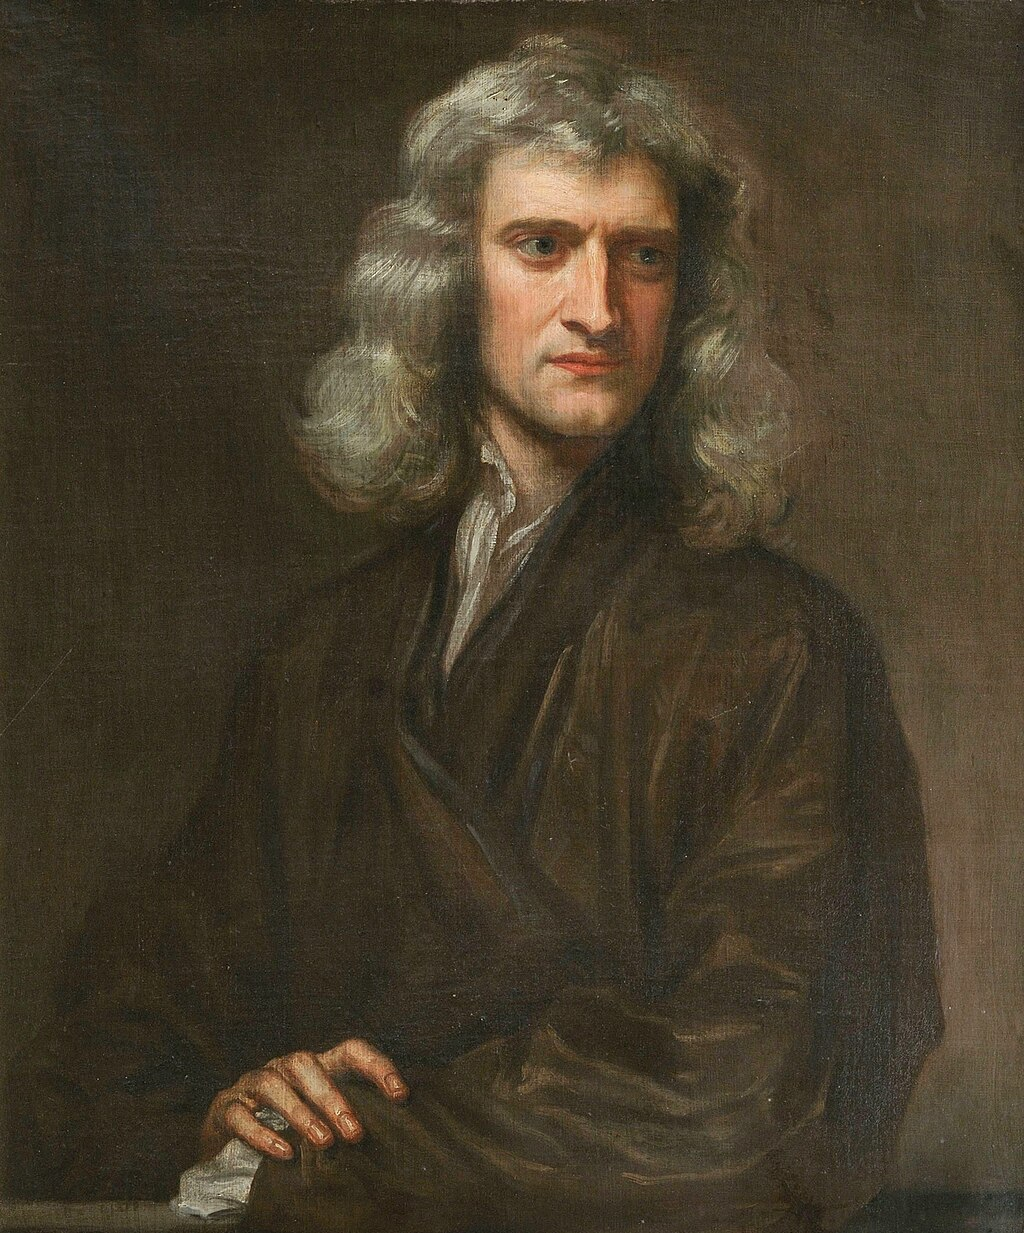
\includegraphics[width=0.5\linewidth]{Images/Portrait_of_Sir_Isaac_Newton,_1689_(brightened).jpg}
    \caption{Portrait of Sir Isaac Newton}
    \label{fig:Newton}
\end{figure}

The history of any kind of mechanics must start with a study of Isaac Newton. Newton is very famous for his description of mechanics based on forces and vectors. However, Newton is also instrumental character in our study of energy mechanics. 

In fact, Newton was instrumental to the development of Calculus of Variations, solving two of the first problems in the subject, the \textit{minimal resistance problem} and the \gls{brachistochrone} problem, which we will further explore in our study of the calculus of variations. It is on these subjects that we will spend most of the time.

Before we explore his contributions in this field, though, an understanding of his work in force-based mechanics and calculus is needed. This background section draws mostly from the text \cite{noauthor_isaac_2017}. Newton's work on variational calculus draws from several different sources, including the original \textit{Principia} and the \cite{goldstine_fermat_1980} chapter of Goldstine.

\subsection{Newton's Beginnings (1643-1661)}
In a story likely familiar to many people who find their interests in the realm of physics and engineering, Newton was born as an unwanted child to both his mother and father.

Born on Christmas Day in 1642 (Early January, 1643 in the modern calendar), Newton was born into an England in the midst of a civil war and full of strife. His father had died 3 months prior to his birth, and he was born prematurely. Newton was unwanted by his own mother, so he was raised by his maternal grandmother, Margery Ayscough.

Needless to say, Isaac Newton's early years were dominated by a lack of control and great turmoil. Thus, Newton took great solace in the isolation and fundamental truth of mathematics. This background in Newton's early life is likely to have had profound influences on his growth into adulthood and his later exploration of math.

Newton, in his years of study before college, had a great fascination for mechanical devices and an understanding of the world around him. It was in 1661 that he gained admittance to the Trinity College in Cambridge, right as the English Civil War was coming to a close.

\subsection{The Newtonian Calculus (1661-1679)}

During his time in college, Newton began his real exploration of mathematics. Newton's first great contribution to mathematics was in his studies of the Binomial theorem, which can give an expansion for a binomial raised to an arbitrary degree. Before Newton, there existed a theorem for the binomial theorem for the integers, $\mathbb{Z}$, which is presented below in \autoref{thm: binomial}.

\begin{theorem}[Binomial theorem]\label{thm: binomial}
    A binomial of form $x+y$ to a power n, where $n\in\mathbb{Z}$, the expansion can be written as:
    $$(x+y)^n=\sum_{k=0}^{n}\binom{n} {k}x^ky^{n-k}$$
    where $\binom{r}{k}$ is defined as:
    $$\binom{n}{k}=\frac{n!}{k!(n-k)!}$$
\end{theorem}

The original scope of this theorem only applies to the integer elements, $\mathbb{Z}$. Newton, however, extended the application of this theorem to the whole of the real numbers, $\mathbb{R}$. Newton's generalized theorem is then:


\begin{theorem}[Generalized Binomial theorem]
    A binomial of form $x+y$ to a power r, where $r\in\mathbb{R}$, the expansion can be written as:
    $$(x+y)^r=\sum_{k-0}^{\infty}\binom{r} {k}x^ry^{r-k}$$
    where $\binom{r}{k}$ is defined as:
    $$\binom{r}{k}=\frac{r(r-1)(r-2)\cdots(r-k+1)}{k!}$$
\end{theorem}

We note here that Newton has introduced an infinite sum! This is one of the first steps towards the methods of calculus. In fact, this equation has applicability towards the definition of the constant $e$, which is very fundemental in our studies of calculus. We can see this by inspection the definition of $e$ as:
$$ \lim_{x\to\infty} \left(1+\frac{1}{n}\right)^n$$
Using Newton's generalized binomial theorem, this infinite limit can be approximated and the value of $e$ can be closely approximated.

Newton continued his work on this subject, graduating in 1665. When Trinity University closed due to the Black Plague in the summer of that year, Newton took his work back home and began the most prolific part of his mathematical career, where he famously had the thought experiment of the apple falling towards the earth. It was during this time that Newton made his famous discoveries in optics and universal gravitation.

It was also during this period of great mathematical bounty that Newton began his studies of calculus. As early as 1665, Newton had methods to compute the derivative and find integral areas of curves. Using the generalized binomial theorem, Newton began to develop the concepts of integration and their applications to physics.

While the Newtonian methods of calculus are largely forgotten today in favor of the notation of Leibniz, it is without a doubt that Newton's contributions to the subject were extraordinary significant. Newton's contributions during this time will play a direct part in our later studies of energy mechanics.

\section{Fermat's Least Time Principle (1662)}
\begin{figure}[ht]
    \centering
    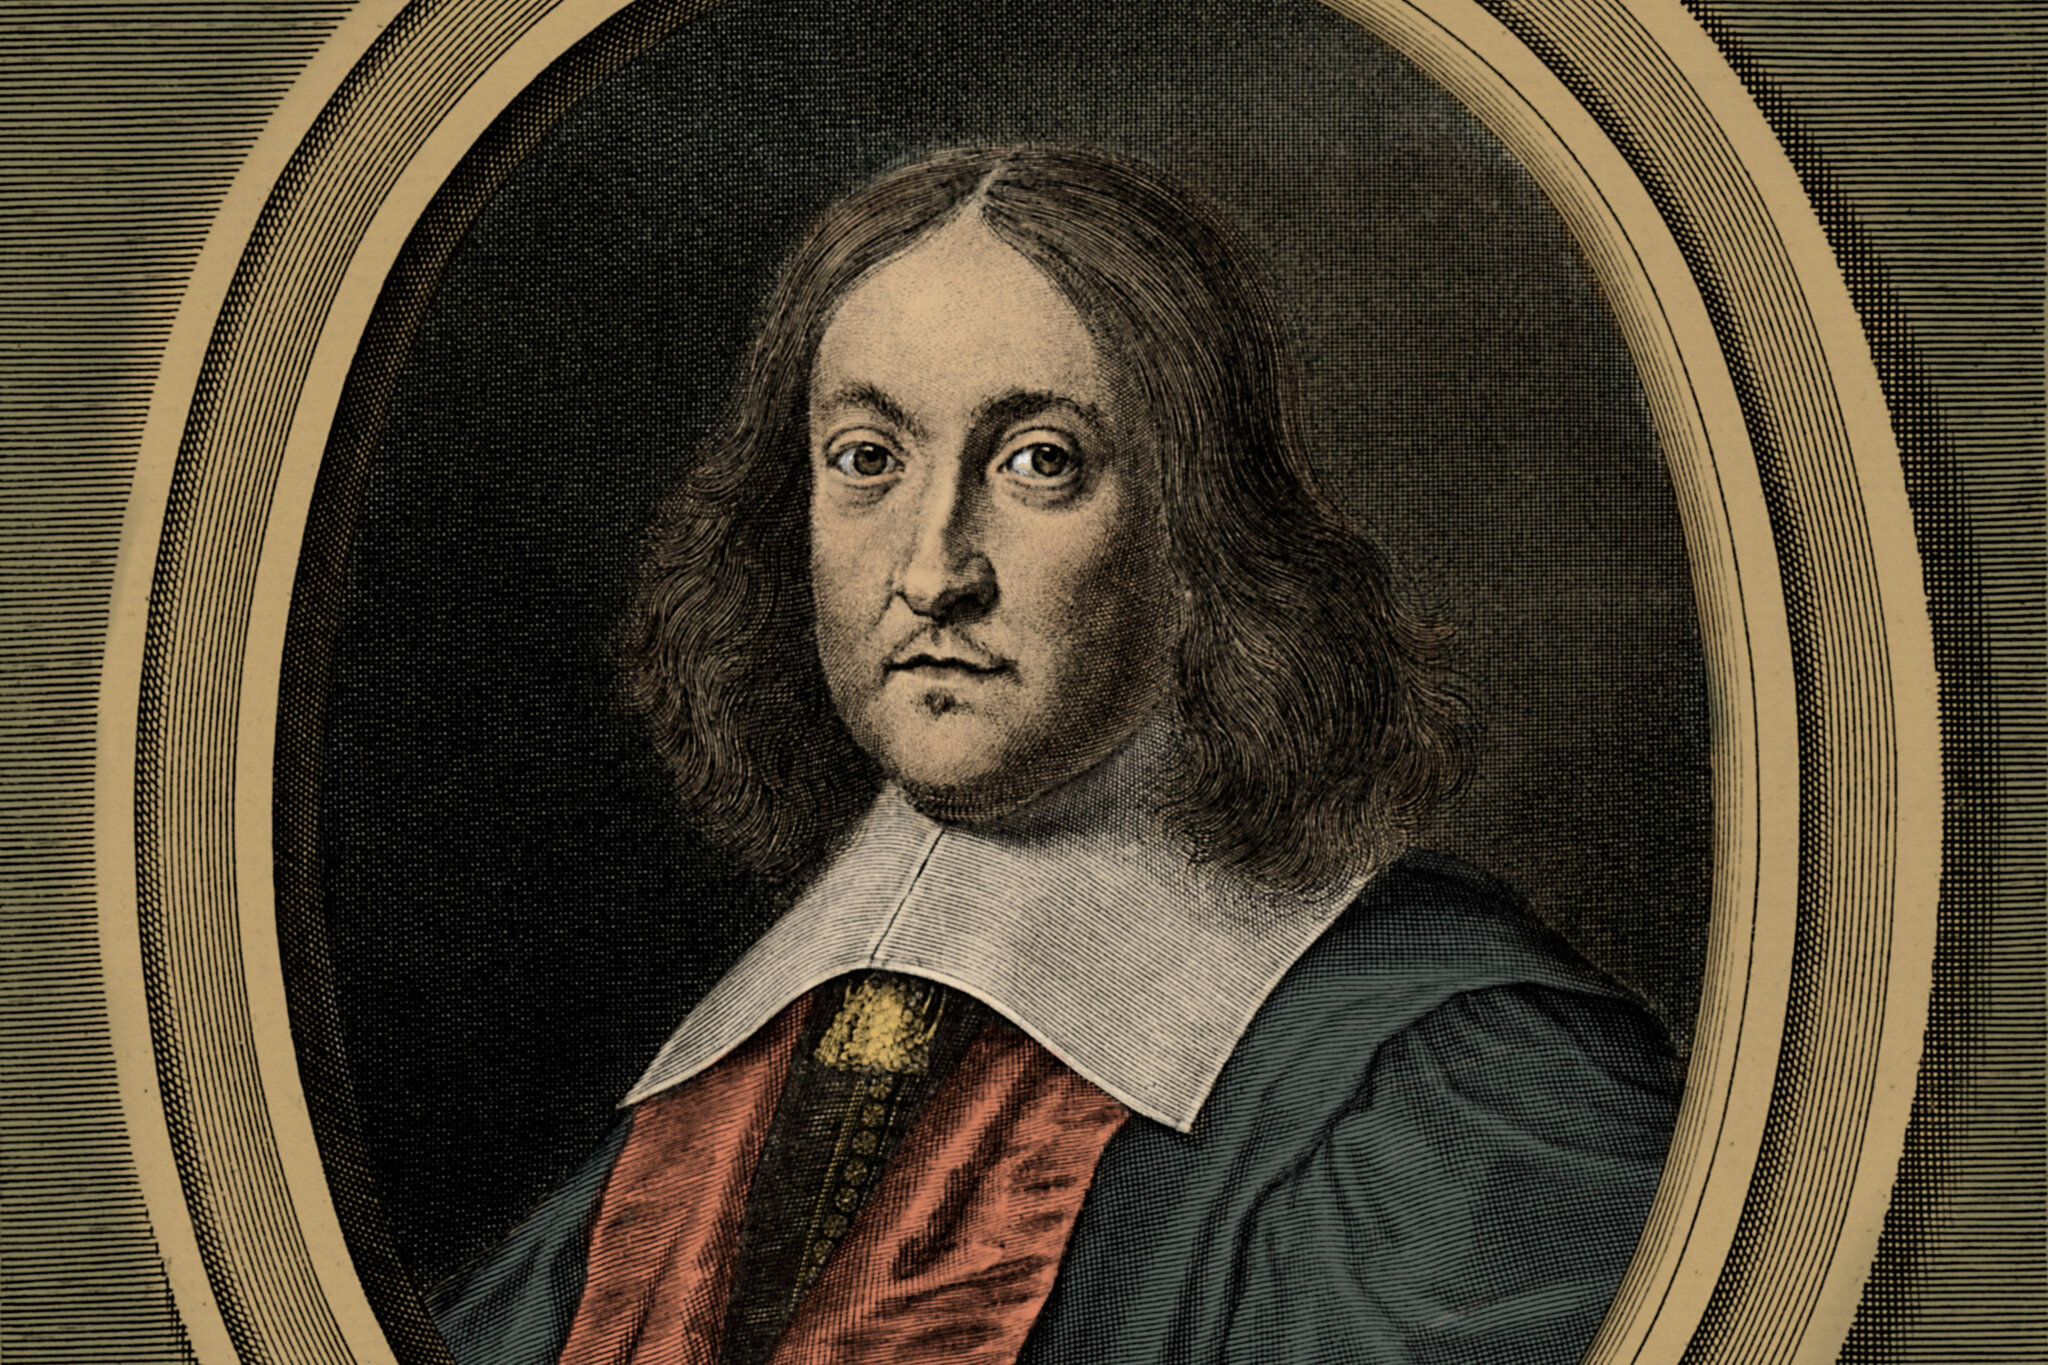
\includegraphics[width=0.75\linewidth]{Images/Fermat.jpg}
    \caption{A portrait of Pierre de Fermat}
    \label{fig:fermat}
\end{figure}
It is in the midst of Newton's most fruitful years that we must talk about Fermat's contributions to the subject of energy mechanics, which predate Newton's earliest contributions by nearly a score.

Fermat is famous in mathematics for \textit{Fermat's Last Theorem}, which remained unsolved for 358 years. A solution involving elliptic curves exists, which you can find an in-depth discussion in \cite{hellegouarch_invitation_2001} (this is entirely irrelevant to our work here). 

His contributions here, however, relate to the so-called \textit{Fermat's Principle of Least Time}. Fermat's biggest insight was the understanding that 'nature operates by means and ways that are easiest and fastest'. Although this way seem a simple statement, it will underlie the physical principle at the root of energy mechanics.

Fermat's Principle of Least Time involves finding a light path such that the time is minimized.\endnote{It can be shown that this is not exactly true, as the only condition required for sufficiency in this problem is that the changes to the variation are of the second-order. Fermat's condition is simply one such case of this. See \cite{feynman_feynman_1963} for more info.}Fermat's set up is as shown in \autoref{fig:least time ray}. Fermat noticed that the light path will refract and change its angle when moving through a medium where the speed of light is slower.

The law of reflection can also be shown from Fermat's Principle, although that will not be done here. It is quite similar to the derivation of the refraction law. If you find an interest in the subject matter here, a much more in-depth discussion in the wonderful Feynman lectures on physics can be found in \cite{feynman_feynman_1963}.

\begin{figure}
    \centering
    

\tikzset{every picture/.style={line width=0.75pt}} %set default line width to 0.75pt        

\begin{tikzpicture}[x=0.75pt,y=0.75pt,yscale=-1,xscale=1]
%uncomment if require: \path (0,300); %set diagram left start at 0, and has height of 300

%Shape: Rectangle [id:dp8879936647316232] 
\draw  [color={rgb, 255:red, 126; green, 219; blue, 222 }  ,draw opacity=0.51 ][fill={rgb, 255:red, 126; green, 219; blue, 222 }  ,fill opacity=0.51 ] (110,130) -- (550,130) -- (550,250) -- (110,250) -- cycle ;
%Straight Lines [id:da9092976870956871] 
\draw    (130,60) -- (350,130) ;
\draw [shift={(130,60)}, rotate = 17.65] [color={rgb, 255:red, 0; green, 0; blue, 0 }  ][fill={rgb, 255:red, 0; green, 0; blue, 0 }  ][line width=0.75]      (0, 0) circle [x radius= 3.35, y radius= 3.35]   ;
%Straight Lines [id:da28057638271133667] 
\draw    (350,130) -- (410,210) ;
\draw [shift={(410,210)}, rotate = 53.13] [color={rgb, 255:red, 0; green, 0; blue, 0 }  ][fill={rgb, 255:red, 0; green, 0; blue, 0 }  ][line width=0.75]      (0, 0) circle [x radius= 3.35, y radius= 3.35]   ;
%Shape: Arc [id:dp9634726814563676] 
\draw  [draw opacity=0] (236.39,93.09) .. controls (252.29,46.98) and (297.15,13.75) .. (350,13.75) -- (350,130) -- cycle ; \draw [color={rgb, 255:red, 74; green, 144; blue, 226 }  ,draw opacity=1 ]   (237.64,89.65) .. controls (254.54,45.34) and (298.47,13.75) .. (350,13.75) ; \draw [shift={(350,13.75)}, rotate = 180] [color={rgb, 255:red, 74; green, 144; blue, 226 }  ,draw opacity=1 ][line width=0.75]    (0,5.03) -- (0,-5.03)   ; \draw [shift={(236.39,93.09)}, rotate = 289.02] [fill={rgb, 255:red, 74; green, 144; blue, 226 }  ,fill opacity=1 ][line width=0.08]  [draw opacity=0] (8.04,-3.86) -- (0,0) -- (8.04,3.86) -- cycle    ;
%Shape: Arc [id:dp3411757437853058] 
\draw  [draw opacity=0] (382.69,173.39) .. controls (373.53,179.9) and (362.23,183.75) .. (350,183.75) -- (350,130) -- cycle ; \draw [color={rgb, 255:red, 74; green, 144; blue, 226 }  ,draw opacity=1 ]   (380.17,175.08) .. controls (371.49,180.56) and (361.13,183.75) .. (350,183.75) ; \draw [shift={(350,183.75)}, rotate = 360] [color={rgb, 255:red, 74; green, 144; blue, 226 }  ,draw opacity=1 ][line width=0.75]    (0,5.03) -- (0,-5.03)   ; \draw [shift={(382.69,173.39)}, rotate = 144.58] [fill={rgb, 255:red, 74; green, 144; blue, 226 }  ,fill opacity=1 ][line width=0.08]  [draw opacity=0] (8.04,-3.86) -- (0,0) -- (8.04,3.86) -- cycle    ;
%Straight Lines [id:da9977458453758269] 
\draw [color={rgb, 255:red, 155; green, 155; blue, 155 }  ,draw opacity=1 ] [dash pattern={on 4.5pt off 4.5pt}]  (350,10) -- (350,250) ;
%Straight Lines [id:da33608457803837766] 
\draw    (130,260) -- (410,260) ;
\draw [shift={(410,260)}, rotate = 180] [color={rgb, 255:red, 0; green, 0; blue, 0 }  ][line width=0.75]    (0,5.59) -- (0,-5.59)   ;
\draw [shift={(130,260)}, rotate = 180] [color={rgb, 255:red, 0; green, 0; blue, 0 }  ][line width=0.75]    (0,5.59) -- (0,-5.59)   ;
%Straight Lines [id:da7724749653392198] 
\draw [color={rgb, 255:red, 218; green, 44; blue, 0 }  ,draw opacity=1 ]   (410,130) -- (410,207) ;
\draw [shift={(410,210)}, rotate = 270] [fill={rgb, 255:red, 218; green, 44; blue, 0 }  ,fill opacity=1 ][line width=0.08]  [draw opacity=0] (8.04,-3.86) -- (0,0) -- (8.04,3.86) -- cycle    ;
\draw [shift={(410,130)}, rotate = 270] [color={rgb, 255:red, 218; green, 44; blue, 0 }  ,draw opacity=1 ][line width=0.75]    (0,5.03) -- (0,-5.03)   ;
%Straight Lines [id:da7478103517482707] 
\draw [color={rgb, 255:red, 218; green, 44; blue, 0 }  ,draw opacity=1 ]   (130,130) -- (130,63) ;
\draw [shift={(130,60)}, rotate = 90] [fill={rgb, 255:red, 218; green, 44; blue, 0 }  ,fill opacity=1 ][line width=0.08]  [draw opacity=0] (8.04,-3.86) -- (0,0) -- (8.04,3.86) -- cycle    ;
%Straight Lines [id:da3656630452978258] 
\draw [color={rgb, 255:red, 218; green, 44; blue, 0 }  ,draw opacity=1 ]   (130,130) -- (347,130) ;
\draw [shift={(350,130)}, rotate = 180] [fill={rgb, 255:red, 218; green, 44; blue, 0 }  ,fill opacity=1 ][line width=0.08]  [draw opacity=0] (8.04,-3.86) -- (0,0) -- (8.04,3.86) -- cycle    ;

% Text Node
\draw (251,22.4) node [anchor=north west][inner sep=0.75pt]    {$\theta _{i}$};
% Text Node
\draw (361,190.4) node [anchor=north west][inner sep=0.75pt]    {$\theta _{r}$};
% Text Node
\draw (270,263.4) node [anchor=north] [inner sep=0.75pt]    {$L$};
% Text Node
\draw (412,170) node [anchor=west] [inner sep=0.75pt]    {$h_{2}$};
% Text Node
\draw (128,95) node [anchor=east] [inner sep=0.75pt]    {$h_{1}$};
% Text Node
\draw (126,54.6) node [anchor=south east] [inner sep=0.75pt]    {$A$};
% Text Node
\draw (412,213.4) node [anchor=north west][inner sep=0.75pt]    {$B$};
% Text Node
\draw (240,126.6) node [anchor=south] [inner sep=0.75pt]    {$x$};

\end{tikzpicture}


    \caption{Fermat's Set-up for the Least Time Problem for a Light Ray}
    \label{fig:least time ray}
\end{figure}

I do not delve into the proof by Fermat, since it uses archaic methods of calculus that are more confusing than enlightening to the modern audience. Fermat's solution is mostly geometric and it involves a geometric proof using the Law of Cosines. 

Instead, I will take a more modern approach which follows roughly along with Fermat. Following the standard procedures of calculus, we will find a minimization of the function by considering the point where the first derivative is zero.

I will present here a modern derivation of this principle, because I believe it makes the later derivations more satisfying and provides a brief introduction to the methodologies of the calculus of variations.

Starting from the set-up shown in \autoref{fig:least time ray}, we can write equations for the time for each of the sections of the light path. To do so, we use the fundemental relationship for velocity:
$$t=\frac{d}{v}$$
Using the definition that the velocity in an optical medium is $v=\frac{c}{n}$, we can write the time for each section. Starting with the section in the lower optical density:
$$t_{upper}=\frac{n_i\sqrt{{h_1}^2+x^2}}{c}$$
And for the more dense optical surface, we do the same:
$$t_{lower}=\frac{n_r\sqrt{{h_2}^2+(l-x)^2}}{c}$$
Altogether, we have a the following relationship:
$$t=\frac{n_i\sqrt{{h_1}^2+x^2}}{c}+\frac{n_r\sqrt{{h_2}^2+(l-x)^2}}{c}$$
We can achieve the desired goal of finding the minimum time by taking the derivative of this time with respect to the variable $x$ and setting it equal to zero as follows:
$$\frac{dt}{dx}=\frac{n_ix}{c\sqrt{{h_1}^2+x^2}}-\frac{n_r(l-x)}{c\sqrt{{h_2}^2+(l-x)^2}}=0$$
A rearrangement leads to the following:
$$\frac{n_ix}{c\sqrt{{h_1}^2+x^2}}=\frac{n_r(l-x)}{c\sqrt{{h_2}^2+(l-x)^2}}$$
Using the established angles $\theta_1$ and $\theta_2$, we can express this relation more simply as:
\begin{gather}
    \color{blue}\boxed{\color{black}n_i\sin\theta_i=n_r\sin\theta_r}\\
    \color{blue}\mathrm{Snell's \ Law}
\end{gather}
We will keep this result in mind, as we will see it again when we solve the problem of the \gls{brachistochrone}.

\subsection{Connection to Quantum Electrodynamics}\label{sec: connection to quantum}
The curious reader may not be fully satisfied with the answer given by Fermat. Why does light take a path that minimizes time? Is there any physical reason for this? In this section we will take a brief aside from the history to answer these questions.

To fully understand this question, we must understand that during Fermat's time there was a rift in the world of physics concerning the behavior of light. Some, such as Newton, believed light to be a particle. Others, led by the prominent dutch mathematician Christaan Huygens, believed that light was a wave.

When we consider light to be a wave, the problem of least time is solved! If the light takes a suboptimal trajectory (that is, a trajectory that takes more time), the wave will destructively interfere with itself. It is only light which takes the shortest path which will constructively interfere and produce a  bright spot! So the riddle is solved. Newton is wrong, and light is in fact a wave! The problem is this: We can measure individual packets of light, photons, arriving at photomultipliers or digital sensors. When a light source gets dimmer, we simply measure fewer numbers of photons, but the energies associated with each one is exactly the same.

So we must again reconsider our viewpoint. Light must showcase both properties to match all of the evidence! Of course, it is now popularly understood that light - and in fact everything else - exhibits both properties in a wave-particle duality.

The existence of this duality alone does not necessarily answer our question, but it gets us on the path to doing so. The true answer to this question remained unknown for nearly 300 years -- until the advent of \gls{qed} in the 1940's, the invention of which would lead Richard Feynman to winning the Nobel Prize in physics.

Of course, explaining a Nobel Prize worthy achievement in physics is no easy task! Luckily, Feynman himself has offered quite a simple explanation of the phenomena of light in his book, \cite{richard_phillips_feynman_qed_1988}. I highly suggest the interested reader to read this book in full (it is quite short and easy to read) to better comprehend this section. Here, I will present only a portion of Feynman's argument to convince you that the least action principle naturally arises from \gls{qed}.

\subsubsection{Mirrors}
Although we earlier made a computation for Snell's Law using Fermat's principle, we will instead take the case of the mirror here. The derivation of the equivalent least time principle for the mirror is left as an exercise, but follows from a similar procedure.
\begin{exercise}
    Using the same methods as were used to derive Snell's Law, find the criteria that minimizes time for the case of a mirror, which reflects light instead of refracting it. The set up for such a mirror system is shown in \autoref{fig:mirror}.
\begin{figure}[H]
    \centering


\tikzset{every picture/.style={line width=0.75pt}} %set default line width to 0.75pt        

\begin{tikzpicture}[x=0.75pt,y=0.75pt,yscale=-1,xscale=1]
%uncomment if require: \path (0,300); %set diagram left start at 0, and has height of 300

%Shape: Rectangle [id:dp6275989944924254] 
\draw  [color={rgb, 255:red, 126; green, 219; blue, 222 }  ,draw opacity=0.51 ][fill={rgb, 255:red, 126; green, 219; blue, 222 }  ,fill opacity=0.51 ] (90,140) -- (570,140) -- (570,260) -- (90,260) -- cycle ;
%Straight Lines [id:da6083348703679279] 
\draw    (110,70) -- (330,140) ;
\draw [shift={(110,70)}, rotate = 17.65] [color={rgb, 255:red, 0; green, 0; blue, 0 }  ][fill={rgb, 255:red, 0; green, 0; blue, 0 }  ][line width=0.75]      (0, 0) circle [x radius= 3.35, y radius= 3.35]   ;
%Shape: Arc [id:dp6990536523303199] 
\draw  [draw opacity=0] (216.39,103.09) .. controls (232.29,56.98) and (277.15,23.75) .. (330,23.75) -- (330,140) -- cycle ; \draw [color={rgb, 255:red, 74; green, 144; blue, 226 }  ,draw opacity=1 ]   (217.64,99.65) .. controls (234.54,55.34) and (278.47,23.75) .. (330,23.75) ; \draw [shift={(330,23.75)}, rotate = 180] [color={rgb, 255:red, 74; green, 144; blue, 226 }  ,draw opacity=1 ][line width=0.75]    (0,5.03) -- (0,-5.03)   ; \draw [shift={(216.39,103.09)}, rotate = 289.02] [fill={rgb, 255:red, 74; green, 144; blue, 226 }  ,fill opacity=1 ][line width=0.08]  [draw opacity=0] (8.04,-3.86) -- (0,0) -- (8.04,3.86) -- cycle    ;
%Straight Lines [id:da21803443744202755] 
\draw [color={rgb, 255:red, 155; green, 155; blue, 155 }  ,draw opacity=1 ] [dash pattern={on 4.5pt off 4.5pt}]  (330,20) -- (330,260) ;
%Straight Lines [id:da33439071823558864] 
\draw    (110,270) -- (550,270) ;
\draw [shift={(550,270)}, rotate = 180] [color={rgb, 255:red, 0; green, 0; blue, 0 }  ][line width=0.75]    (0,5.59) -- (0,-5.59)   ;
\draw [shift={(110,270)}, rotate = 180] [color={rgb, 255:red, 0; green, 0; blue, 0 }  ][line width=0.75]    (0,5.59) -- (0,-5.59)   ;
%Straight Lines [id:da48893176676953176] 
\draw [color={rgb, 255:red, 218; green, 44; blue, 0 }  ,draw opacity=1 ]   (110,140) -- (110,73) ;
\draw [shift={(110,70)}, rotate = 90] [fill={rgb, 255:red, 218; green, 44; blue, 0 }  ,fill opacity=1 ][line width=0.08]  [draw opacity=0] (8.04,-3.86) -- (0,0) -- (8.04,3.86) -- cycle    ;
%Straight Lines [id:da28787272817377096] 
\draw [color={rgb, 255:red, 218; green, 44; blue, 0 }  ,draw opacity=1 ]   (110,140) -- (327,140) ;
\draw [shift={(330,140)}, rotate = 180] [fill={rgb, 255:red, 218; green, 44; blue, 0 }  ,fill opacity=1 ][line width=0.08]  [draw opacity=0] (8.04,-3.86) -- (0,0) -- (8.04,3.86) -- cycle    ;
%Straight Lines [id:da5717809459497747] 
\draw    (550,70) -- (330,140) ;
\draw [shift={(550,70)}, rotate = 162.35] [color={rgb, 255:red, 0; green, 0; blue, 0 }  ][fill={rgb, 255:red, 0; green, 0; blue, 0 }  ][line width=0.75]      (0, 0) circle [x radius= 3.35, y radius= 3.35]   ;
%Shape: Arc [id:dp08924222560062933] 
\draw  [draw opacity=0] (330,23.75) .. controls (330,23.75) and (330,23.75) .. (330,23.75) .. controls (382.85,23.75) and (427.71,56.98) .. (443.61,103.09) -- (330,140) -- cycle ; \draw [color={rgb, 255:red, 74; green, 144; blue, 226 }  ,draw opacity=1 ]   (330,23.75) .. controls (381.8,23.75) and (425.91,55.66) .. (442.62,100.34) ; \draw [shift={(443.61,103.09)}, rotate = 250.98] [fill={rgb, 255:red, 74; green, 144; blue, 226 }  ,fill opacity=1 ][line width=0.08]  [draw opacity=0] (8.04,-3.86) -- (0,0) -- (8.04,3.86) -- cycle    ; 

% Text Node
\draw (231,32.4) node [anchor=north west][inner sep=0.75pt]    {$\theta _{i}$};
% Text Node
\draw (330,273.4) node [anchor=north] [inner sep=0.75pt]    {$L$};
% Text Node
\draw (108,105) node [anchor=east] [inner sep=0.75pt]    {$h_{1}$};
% Text Node
\draw (106,64.6) node [anchor=south east] [inner sep=0.75pt]    {$A$};
% Text Node
\draw (557,52.4) node [anchor=north west][inner sep=0.75pt]    {$B$};
% Text Node
\draw (220,136.6) node [anchor=south] [inner sep=0.75pt]    {$x$};
% Text Node
\draw (406,31.4) node [anchor=north west][inner sep=0.75pt]    {$\theta _{f}$};


\end{tikzpicture}

    \caption{Mirror Set-Up}
    \label{fig:mirror}
\end{figure}
\end{exercise}

Readers who carefully perform the derivation above using the methods shown before will find that in the case of the mirror, $\theta_i=\theta_f$. That is, the incident angle is equal to the outgoing angle. In our previous derivations, we showed this to be a consequence of the principle of least time.

If we think of the problem more `democratically', we shouldn't give any preference to any one path though! Let's consider all of the straight line paths that light can take. A few of these paths are shown in \autoref{fig:light traj}.
\begin{figure}[ht]
    \centering

% Pattern Info
 
\tikzset{
pattern size/.store in=\mcSize, 
pattern size = 5pt,
pattern thickness/.store in=\mcThickness, 
pattern thickness = 0.3pt,
pattern radius/.store in=\mcRadius, 
pattern radius = 1pt}
\makeatletter
\pgfutil@ifundefined{pgf@pattern@name@_6b3jznvkh}{
\pgfdeclarepatternformonly[\mcThickness,\mcSize]{_6b3jznvkh}
{\pgfqpoint{0pt}{0pt}}
{\pgfpoint{\mcSize+\mcThickness}{\mcSize+\mcThickness}}
{\pgfpoint{\mcSize}{\mcSize}}
{
\pgfsetcolor{\tikz@pattern@color}
\pgfsetlinewidth{\mcThickness}
\pgfpathmoveto{\pgfqpoint{0pt}{0pt}}
\pgfpathlineto{\pgfpoint{\mcSize+\mcThickness}{\mcSize+\mcThickness}}
\pgfusepath{stroke}
}}
\makeatother
\tikzset{every picture/.style={line width=0.75pt}} %set default line width to 0.75pt        

\begin{tikzpicture}[x=0.75pt,y=0.75pt,yscale=-1,xscale=1]
%uncomment if require: \path (0,300); %set diagram left start at 0, and has height of 300

%Shape: Rectangle [id:dp13216032235189357] 
\draw  [color={rgb, 255:red, 126; green, 219; blue, 222 }  ,draw opacity=0.51 ][fill={rgb, 255:red, 126; green, 219; blue, 222 }  ,fill opacity=0.51 ] (100,240) -- (560,240) -- (560,280) -- (100,280) -- cycle ;
%Shape: Rectangle [id:dp7152402004015799] 
\draw  [pattern=_6b3jznvkh,pattern size=7.5pt,pattern thickness=0.75pt,pattern radius=0pt, pattern color={rgb, 255:red, 0; green, 0; blue, 0}] (320,130) -- (340,130) -- (340,170) -- (320,170) -- cycle ;
%Straight Lines [id:da14645204907035414] 
\draw [line width=0.75]    (140,160) -- (330,240) ;
%Straight Lines [id:da5333244615267384] 
\draw [line width=0.75]    (520,160) -- (330,240) ;
%Straight Lines [id:da19778015344004796] 
\draw [line width=0.75]    (140,160) -- (240,240) ;
%Straight Lines [id:da47608518269163747] 
\draw [line width=0.75]    (520,160) -- (240,240) ;
%Straight Lines [id:da14756293959452693] 
\draw [line width=0.75]    (520,160) -- (420,240) ;
%Straight Lines [id:da7018685323723184] 
\draw [line width=0.75]    (140,160) -- (420,240) ;
%Straight Lines [id:da7703911392020962] 
\draw [line width=0.75]    (140,160) -- (180,240) ;
%Straight Lines [id:da3928605678682944] 
\draw [line width=0.75]    (520,160) -- (180,240) ;
%Straight Lines [id:da5605057304874714] 
\draw [line width=0.75]    (520,160) -- (480,240) ;
%Straight Lines [id:da19372382419577583] 
\draw [line width=0.75]    (140,160) -- (480,240) ;

% Text Node
\draw (121,142.4) node [anchor=north west][inner sep=0.75pt]    {$A$};
% Text Node
\draw (527,142.4) node [anchor=north west][inner sep=0.75pt]    {$B$};


\end{tikzpicture}
    \caption{Possible trajectories of light across a mirror}
    \label{fig:light traj}
\end{figure}

Of course, we know from experience that mirrors do not show reflections like this. If they did, we could look from point $A$ at any angle and we would see $B$ centered in the view. There must be something wrong with our model! And there is: we are missing a key component called the phase of the light. Essentially, the phase measures the `direction' of the light (this description will suffice for our purposes). We can think of the phase of the light as a little clock that moves with the light. The clock hand starts pointing straight up at point $A$, and it winds around at a constant rate until the photon reaches point $B$, at that point, we measure the direction the clock hand is pointing. This direction will be a vector with a length of 1, but the direction will change based on the time duration!

So, if we take phase into consideration, we get a new picture of the phenomenon, which is shown in \autoref{fig:polarization paths}. What is shown is the time that it takes each ray of light to reach point $B$ based on the point where it hits the mirror. These are marked with a red marker below the point of intersection with the mirror.

\begin{figure}[ht]
    \centering



% Pattern Info
 
\tikzset{
pattern size/.store in=\mcSize, 
pattern size = 5pt,
pattern thickness/.store in=\mcThickness, 
pattern thickness = 0.3pt,
pattern radius/.store in=\mcRadius, 
pattern radius = 1pt}
\makeatletter
\pgfutil@ifundefined{pgf@pattern@name@_bnexa4sr6}{
\pgfdeclarepatternformonly[\mcThickness,\mcSize]{_bnexa4sr6}
{\pgfqpoint{0pt}{0pt}}
{\pgfpoint{\mcSize+\mcThickness}{\mcSize+\mcThickness}}
{\pgfpoint{\mcSize}{\mcSize}}
{
\pgfsetcolor{\tikz@pattern@color}
\pgfsetlinewidth{\mcThickness}
\pgfpathmoveto{\pgfqpoint{0pt}{0pt}}
\pgfpathlineto{\pgfpoint{\mcSize+\mcThickness}{\mcSize+\mcThickness}}
\pgfusepath{stroke}
}}
\makeatother
\tikzset{every picture/.style={line width=0.75pt}} %set default line width to 0.75pt        

\begin{tikzpicture}[x=0.75pt,y=0.75pt,yscale=-1,xscale=1]
%uncomment if require: \path (0,415); %set diagram left start at 0, and has height of 415

%Shape: Rectangle [id:dp13216032235189357] 
\draw  [color={rgb, 255:red, 126; green, 219; blue, 222 }  ,draw opacity=0.51 ][fill={rgb, 255:red, 126; green, 219; blue, 222 }  ,fill opacity=0.51 ] (100,130) -- (560,130) -- (560,170) -- (100,170) -- cycle ;
%Shape: Rectangle [id:dp7152402004015799] 
\draw  [pattern=_bnexa4sr6,pattern size=7.5pt,pattern thickness=0.75pt,pattern radius=0pt, pattern color={rgb, 255:red, 0; green, 0; blue, 0}] (320,20) -- (340,20) -- (340,60) -- (320,60) -- cycle ;
%Straight Lines [id:da14645204907035414] 
\draw [line width=0.75]    (140,50) -- (330,130) ;
%Straight Lines [id:da5333244615267384] 
\draw [line width=0.75]    (520,50) -- (330,130) ;
%Straight Lines [id:da19778015344004796] 
\draw [line width=0.75]    (140,50) -- (240,130) ;
%Straight Lines [id:da47608518269163747] 
\draw [line width=0.75]    (520,50) -- (240,130) ;
%Straight Lines [id:da14756293959452693] 
\draw [line width=0.75]    (520,50) -- (420,130) ;
%Straight Lines [id:da7018685323723184] 
\draw [line width=0.75]    (140,50) -- (420,130) ;
%Straight Lines [id:da7703911392020962] 
\draw [line width=0.75]    (140,50) -- (180,130) ;
%Straight Lines [id:da3928605678682944] 
\draw [line width=0.75]    (520,50) -- (180,130) ;
%Straight Lines [id:da5605057304874714] 
\draw [line width=0.75]    (520,50) -- (480,130) ;
%Straight Lines [id:da19372382419577583] 
\draw [line width=0.75]    (140,50) -- (480,130) ;
%Shape: Arc [id:dp8977631415857631] 
\draw  [draw opacity=0] (499.01,206.52) .. controls (463.55,238.66) and (401.11,260) .. (330,260) .. controls (258.89,260) and (196.45,238.66) .. (160.99,206.52) -- (330,145) -- cycle ; \draw   (499.01,206.52) .. controls (463.55,238.66) and (401.11,260) .. (330,260) .. controls (258.89,260) and (196.45,238.66) .. (160.99,206.52) ;  
%Straight Lines [id:da5752570776084447] 
\draw [color={rgb, 255:red, 218; green, 44; blue, 0 }  ,draw opacity=1 ]   (180,221) ;
\draw [shift={(180,221)}, rotate = 45] [color={rgb, 255:red, 218; green, 44; blue, 0 }  ,draw opacity=1 ][line width=0.75]    (-6.15,0) -- (6.15,0)(0,6.15) -- (0,-6.15)   ;
\draw [shift={(180,221)}, rotate = 45] [color={rgb, 255:red, 218; green, 44; blue, 0 }  ,draw opacity=1 ][line width=0.75]    (-6.15,0) -- (6.15,0)(0,6.15) -- (0,-6.15)   ;
%Straight Lines [id:da1280857343863272] 
\draw [color={rgb, 255:red, 218; green, 44; blue, 0 }  ,draw opacity=1 ]   (240,248) ;
\draw [shift={(240,248)}, rotate = 45] [color={rgb, 255:red, 218; green, 44; blue, 0 }  ,draw opacity=1 ][line width=0.75]    (-6.15,0) -- (6.15,0)(0,6.15) -- (0,-6.15)   ;
\draw [shift={(240,248)}, rotate = 45] [color={rgb, 255:red, 218; green, 44; blue, 0 }  ,draw opacity=1 ][line width=0.75]    (-6.15,0) -- (6.15,0)(0,6.15) -- (0,-6.15)   ;
%Straight Lines [id:da08965219408030722] 
\draw [color={rgb, 255:red, 218; green, 44; blue, 0 }  ,draw opacity=1 ]   (330,260) ;
\draw [shift={(330,260)}, rotate = 45] [color={rgb, 255:red, 218; green, 44; blue, 0 }  ,draw opacity=1 ][line width=0.75]    (-6.15,0) -- (6.15,0)(0,6.15) -- (0,-6.15)   ;
\draw [shift={(330,260)}, rotate = 45] [color={rgb, 255:red, 218; green, 44; blue, 0 }  ,draw opacity=1 ][line width=0.75]    (-6.15,0) -- (6.15,0)(0,6.15) -- (0,-6.15)   ;
%Straight Lines [id:da37818780636602134] 
\draw [color={rgb, 255:red, 218; green, 44; blue, 0 }  ,draw opacity=1 ]   (480,221) ;
\draw [shift={(480,221)}, rotate = 45] [color={rgb, 255:red, 218; green, 44; blue, 0 }  ,draw opacity=1 ][line width=0.75]    (-6.15,0) -- (6.15,0)(0,6.15) -- (0,-6.15)   ;
\draw [shift={(480,221)}, rotate = 45] [color={rgb, 255:red, 218; green, 44; blue, 0 }  ,draw opacity=1 ][line width=0.75]    (-6.15,0) -- (6.15,0)(0,6.15) -- (0,-6.15)   ;
%Straight Lines [id:da47667957118212323] 
\draw [color={rgb, 255:red, 218; green, 44; blue, 0 }  ,draw opacity=1 ]   (420,248) ;
\draw [shift={(420,248)}, rotate = 45] [color={rgb, 255:red, 218; green, 44; blue, 0 }  ,draw opacity=1 ][line width=0.75]    (-6.15,0) -- (6.15,0)(0,6.15) -- (0,-6.15)   ;
\draw [shift={(420,248)}, rotate = 45] [color={rgb, 255:red, 218; green, 44; blue, 0 }  ,draw opacity=1 ][line width=0.75]    (-6.15,0) -- (6.15,0)(0,6.15) -- (0,-6.15)   ;
%Straight Lines [id:da007076057060994345] 
\draw    (130,190) -- (130,270) ;
%Straight Lines [id:da14315018255479806] 
\draw    (530,270) -- (130,270) ;
%Straight Lines [id:da15061696183681172] 
\draw [line width=0.75]    (140,50) -- (310,130) ;
%Straight Lines [id:da2002580638128295] 
\draw [line width=0.75]    (520,50) -- (310,130) ;
%Straight Lines [id:da32478234854039456] 
\draw [line width=0.75]    (140,50) -- (350,130) ;
%Straight Lines [id:da23492277853880672] 
\draw [line width=0.75]    (520,50) -- (350,130) ;
%Straight Lines [id:da4384311212275247] 
\draw [color={rgb, 255:red, 218; green, 44; blue, 0 }  ,draw opacity=1 ]   (310,259) ;
\draw [shift={(310,259)}, rotate = 45] [color={rgb, 255:red, 218; green, 44; blue, 0 }  ,draw opacity=1 ][line width=0.75]    (-6.15,0) -- (6.15,0)(0,6.15) -- (0,-6.15)   ;
\draw [shift={(310,259)}, rotate = 45] [color={rgb, 255:red, 218; green, 44; blue, 0 }  ,draw opacity=1 ][line width=0.75]    (-6.15,0) -- (6.15,0)(0,6.15) -- (0,-6.15)   ;
%Straight Lines [id:da09345020430918904] 
\draw [color={rgb, 255:red, 218; green, 44; blue, 0 }  ,draw opacity=1 ]   (350,260) ;
\draw [shift={(350,260)}, rotate = 45] [color={rgb, 255:red, 218; green, 44; blue, 0 }  ,draw opacity=1 ][line width=0.75]    (-6.15,0) -- (6.15,0)(0,6.15) -- (0,-6.15)   ;
\draw [shift={(350,260)}, rotate = 45] [color={rgb, 255:red, 218; green, 44; blue, 0 }  ,draw opacity=1 ][line width=0.75]    (-6.15,0) -- (6.15,0)(0,6.15) -- (0,-6.15)   ;
%Straight Lines [id:da5924170533496909] 
\draw    (170,290) -- (188,290) ;
\draw [shift={(190,290)}, rotate = 180] [color={rgb, 255:red, 0; green, 0; blue, 0 }  ][line width=0.75]    (7.65,-2.3) .. controls (4.86,-0.97) and (2.31,-0.21) .. (0,0) .. controls (2.31,0.21) and (4.86,0.98) .. (7.65,2.3)   ;
%Straight Lines [id:da5827611285701653] 
\draw    (470,290) -- (488,290) ;
\draw [shift={(490,290)}, rotate = 180] [color={rgb, 255:red, 0; green, 0; blue, 0 }  ][line width=0.75]    (7.65,-2.3) .. controls (4.86,-0.97) and (2.31,-0.21) .. (0,0) .. controls (2.31,0.21) and (4.86,0.98) .. (7.65,2.3)   ;
%Straight Lines [id:da6566762407882489] 
\draw    (246,298) -- (232.46,285.36) ;
\draw [shift={(231,284)}, rotate = 43.03] [color={rgb, 255:red, 0; green, 0; blue, 0 }  ][line width=0.75]    (7.65,-2.3) .. controls (4.86,-0.97) and (2.31,-0.21) .. (0,0) .. controls (2.31,0.21) and (4.86,0.98) .. (7.65,2.3)   ;
%Straight Lines [id:da5408338245488791] 
\draw    (427,298) -- (413.46,285.36) ;
\draw [shift={(412,284)}, rotate = 43.03] [color={rgb, 255:red, 0; green, 0; blue, 0 }  ][line width=0.75]    (7.65,-2.3) .. controls (4.86,-0.97) and (2.31,-0.21) .. (0,0) .. controls (2.31,0.21) and (4.86,0.98) .. (7.65,2.3)   ;
%Straight Lines [id:da4955723577989215] 
\draw    (302,295) -- (313.64,282.47) ;
\draw [shift={(315,281)}, rotate = 132.88] [color={rgb, 255:red, 0; green, 0; blue, 0 }  ][line width=0.75]    (7.65,-2.3) .. controls (4.86,-0.97) and (2.31,-0.21) .. (0,0) .. controls (2.31,0.21) and (4.86,0.98) .. (7.65,2.3)   ;
%Straight Lines [id:da5611205109573854] 
\draw    (323,295) -- (337.45,283.26) ;
\draw [shift={(339,282)}, rotate = 140.91] [color={rgb, 255:red, 0; green, 0; blue, 0 }  ][line width=0.75]    (7.65,-2.3) .. controls (4.86,-0.97) and (2.31,-0.21) .. (0,0) .. controls (2.31,0.21) and (4.86,0.98) .. (7.65,2.3)   ;
%Straight Lines [id:da876842810834746] 
\draw    (344,294) -- (361.27,284) ;
\draw [shift={(363,283)}, rotate = 149.93] [color={rgb, 255:red, 0; green, 0; blue, 0 }  ][line width=0.75]    (7.65,-2.3) .. controls (4.86,-0.97) and (2.31,-0.21) .. (0,0) .. controls (2.31,0.21) and (4.86,0.98) .. (7.65,2.3)   ;
%Straight Lines [id:da1460915799548117] 
\draw    (302,380) -- (320,380) ;
\draw [shift={(322,380)}, rotate = 180] [color={rgb, 255:red, 0; green, 0; blue, 0 }  ][line width=0.75]    (7.65,-2.3) .. controls (4.86,-0.97) and (2.31,-0.21) .. (0,0) .. controls (2.31,0.21) and (4.86,0.98) .. (7.65,2.3)   ;
%Straight Lines [id:da0417350409731837] 
\draw    (340,314) -- (358,314) ;
\draw [shift={(360,314)}, rotate = 180] [color={rgb, 255:red, 0; green, 0; blue, 0 }  ][line width=0.75]    (7.65,-2.3) .. controls (4.86,-0.97) and (2.31,-0.21) .. (0,0) .. controls (2.31,0.21) and (4.86,0.98) .. (7.65,2.3)   ;
%Straight Lines [id:da9009267203358027] 
\draw    (322,380) -- (308.46,367.36) ;
\draw [shift={(307,366)}, rotate = 43.03] [color={rgb, 255:red, 0; green, 0; blue, 0 }  ][line width=0.75]    (7.65,-2.3) .. controls (4.86,-0.97) and (2.31,-0.21) .. (0,0) .. controls (2.31,0.21) and (4.86,0.98) .. (7.65,2.3)   ;
%Straight Lines [id:da6327757626913345] 
\draw    (355,328) -- (341.46,315.36) ;
\draw [shift={(340,314)}, rotate = 43.03] [color={rgb, 255:red, 0; green, 0; blue, 0 }  ][line width=0.75]    (7.65,-2.3) .. controls (4.86,-0.97) and (2.31,-0.21) .. (0,0) .. controls (2.31,0.21) and (4.86,0.98) .. (7.65,2.3)   ;
%Straight Lines [id:da8821395763135093] 
\draw    (307,366) -- (318.64,353.47) ;
\draw [shift={(320,352)}, rotate = 132.88] [color={rgb, 255:red, 0; green, 0; blue, 0 }  ][line width=0.75]    (7.65,-2.3) .. controls (4.86,-0.97) and (2.31,-0.21) .. (0,0) .. controls (2.31,0.21) and (4.86,0.98) .. (7.65,2.3)   ;
%Straight Lines [id:da20662846712873373] 
\draw    (320,352) -- (334.45,340.26) ;
\draw [shift={(336,339)}, rotate = 140.91] [color={rgb, 255:red, 0; green, 0; blue, 0 }  ][line width=0.75]    (7.65,-2.3) .. controls (4.86,-0.97) and (2.31,-0.21) .. (0,0) .. controls (2.31,0.21) and (4.86,0.98) .. (7.65,2.3)   ;
%Straight Lines [id:da35979068209407283] 
\draw    (336,339) -- (353.27,329) ;
\draw [shift={(355,328)}, rotate = 149.93] [color={rgb, 255:red, 0; green, 0; blue, 0 }  ][line width=0.75]    (7.65,-2.3) .. controls (4.86,-0.97) and (2.31,-0.21) .. (0,0) .. controls (2.31,0.21) and (4.86,0.98) .. (7.65,2.3)   ;
%Straight Lines [id:da4924995281799577] 
\draw [color={rgb, 255:red, 218; green, 44; blue, 0 }  ,draw opacity=1 ][line width=1.5]    (302,380) -- (358.02,316.25) ;
\draw [shift={(360,314)}, rotate = 131.31] [color={rgb, 255:red, 218; green, 44; blue, 0 }  ,draw opacity=1 ][line width=1.5]    (9.95,-2.99) .. controls (6.32,-1.27) and (3.01,-0.27) .. (0,0) .. controls (3.01,0.27) and (6.32,1.27) .. (9.95,2.99)   ;

% Text Node
\draw (121,32.4) node [anchor=north west][inner sep=0.75pt]    {$A$};
% Text Node
\draw (527,32.4) node [anchor=north west][inner sep=0.75pt]    {$B$};
% Text Node
\draw (95,212) node [anchor=north west][inner sep=0.75pt]  [font=\small] [align=left] {Time};


\end{tikzpicture}

    \caption{Phase of light for different paths}
    \label{fig:polarization paths}
\end{figure}

The final phase of the light upon reaching point $B$ is shown below this image. The light rotates very rapidly, so a difference in time will cause large changes in the phase of the light. For paths that are far away from the center, these time differences create arrows that point in seemingly random directions! The result of this is that, on average, these arrows tend to cancel each other out.

However, for paths that are close to the path of least time, we can move the intersection point left and right and the amount of time taken doesn't change much at all! This occurs, of course, because we are at a local minimum of the function, where the derivative is 0. When we look at the vectors for these portions, we find that the phase for each of these is almost identical! So we find that these paths near the path of least time have vectors that are all very similar to each other.

The last step in this process is to add all of the vectors together to generate a final vector. The square of this final vector is representative of the probability that light reaches point $B$. By adding all of the vectors from before together, we can see that the largest contribution to the final vector comes from the portion in the middle. In fact, some of the portions near the outside can cancel each other out so that they have almost no effect.

Although the methodology described above is perfectly sound, the angular and time differences described here are quite exaggerated. In reality, even paths deviating by less than a degree from the ideal path tend to cancel each other out for visible light. This is a result of the frequency of light being so high that phase shifts occur on the order of picoseconds.

If you want to gain a better understanding of this relationship, an interactive MATLAB script "Mirror.m" in \autoref{sec: Quantum Deriv Mirror} will run a simulation of this scenario. There, you can see how the vectors add for our demonstration model and also for a real physical system with a variable number of elements. The main thing to note is that the effects occur on a much smaller scale for a true physical system. However, we will still see the same effects arise and the form spiral patterns near the ends, where the vectors tend to cancel each other out. Altogether, they form a very beautiful spiral reminiscent of soundholes of a string instrument. Again, only the components near the path of least time add together! So, on the large scale, we say that light does indeed take the path of least time, even though we can show on the quantum scale that it is free to do anything!

\begin{figure}
    \centering
\includesvg[width=.625\linewidth]{Scripts/MirrorVectors.svg}
    \caption{Vector Representation of Mirror}
    \label{fig:mirror vec 2}
\end{figure}

Lastly, note that the actual computation involves computing every possible path that light can take! This includes all of the other infinitely many straight line paths that we ignored, but also paths that are curved in any arbitrary manner. This is quite difficult to do, so I have stuck with the straight-line examples here. As it turns out, both yield the same final answer.

Another simplification you may have noticed is that the magnitude of the final vector arrow squared is the probability. However, we have given each component a length of 1! So if we add infinitely many of these together, the total probability will go to $\infty$, which is obviously incorrect. This is a problem in \gls{qed} called renormalization. Despite some of these challenges, \gls{qed} still provides a very nice framework that allows us to understand why the principle of least time holds.

\section{Principia (1687)}
We may return from our foray into \gls{qed} to once again discuss the contributions of Isaac Newton. It is in \textit{Principia} that we find the first evidences of Newton's contributions to the field of energy mechanics. It is Newton's work in the \textit{Principia} that most scholars agree are the first real works of the calculus of variations.

In 1685, Newton formulated the \textit{minimal resistance problem}. In essence, this problem involves finding a solid of revolution for which the object produces a minimal drag. In Newton's time, no solidified theories of fluid dynamics had been formulated, so Newton suggested a fluid that is `a rare medium of very small quiescent particles of equal magnitude and freely disposed at equal distances from one other'. Although this fluid is not at all reminiscent of a real fluid, it still remains a useful exercise in the study of the calculus of variations.

The major advancement in this problem came from Newton's formulation to solve it. Skipping a few steps of the geometry, Newton came up with a simple integral to represent the drag of an object:
$$\int_{t_1}^{t_2}{\frac{y\dot{y}^3dt}{\dot{x}^2+\dot{y}^2}}$$
In this equation, Newton has parameterized the curve in terms of the variable $t$ and expressed the derivatives of $x$ and $y$ with respect to $t$ as $\dot{x}$ and $\dot{y}$.

As we will see later, this integral is something that we will call a \gls{functional}, and it is the quantity which we want to minimize. 

Newton, despite sharing this result in his \textit{Principia}, did not share his methodology in the original publication. It was not until 1691, when Huygens began independent study of the problem, that anyone had shed any light on the methods of solving the problem. The text, however, still inspired the idea of the functional and began the further exploration of the subject of calculus of variations.

With the idea of the functional created and a methodology to solve problems in the calculus of variations, the next major step in the subject came with the \gls{brachistochrone} problem.

\section{Brachistochrone (1696)}

In June of 1696, nearly a decade after Newton's initial foray into the calculus of variations, John Bernoulli challenged the mathematical world to solve the problem of the \gls{brachistochrone} - a word coming from Greek, meaning 'shortest time'. In its simplest description, the problem involves finding a curve for which a frictionless bead will descend the fastest. A simple diagram of the system is reproduced in \autoref{fig:Brachistochrone}. 

\begin{figure}[ht]
    \centering



\tikzset{every picture/.style={line width=0.75pt}} %set default line width to 0.75pt        

\begin{tikzpicture}[x=0.75pt,y=0.75pt,yscale=-1,xscale=1]
%uncomment if require: \path (0,300); %set diagram left start at 0, and has height of 300

%Curve Lines [id:da5626290173929862] 
\draw [line width=2.25]    (226,80) .. controls (224.23,164.47) and (303.23,269.47) .. (426,230) ;
%Shape: Circle [id:dp16005060334035148] 
\draw  [color={rgb, 255:red, 74; green, 144; blue, 226 }  ,draw opacity=1 ][fill={rgb, 255:red, 74; green, 144; blue, 226 }  ,fill opacity=1 ] (228,88) .. controls (228,85.24) and (230.24,83) .. (233,83) .. controls (235.76,83) and (238,85.24) .. (238,88) .. controls (238,90.76) and (235.76,93) .. (233,93) .. controls (230.24,93) and (228,90.76) .. (228,88) -- cycle ;
%Straight Lines [id:da9179973387326911] 
\draw    (136,80) -- (136,118) ;
\draw [shift={(136,120)}, rotate = 270] [color={rgb, 255:red, 0; green, 0; blue, 0 }  ][line width=0.75]    (7.65,-2.3) .. controls (4.86,-0.97) and (2.31,-0.21) .. (0,0) .. controls (2.31,0.21) and (4.86,0.98) .. (7.65,2.3)   ;
%Straight Lines [id:da23565770066909053] 
\draw    (136,80) -- (174,80) ;
\draw [shift={(176,80)}, rotate = 180] [color={rgb, 255:red, 0; green, 0; blue, 0 }  ][line width=0.75]    (7.65,-2.3) .. controls (4.86,-0.97) and (2.31,-0.21) .. (0,0) .. controls (2.31,0.21) and (4.86,0.98) .. (7.65,2.3)   ;

% Text Node
\draw (207,72.4) node [anchor=north west][inner sep=0.75pt]    {$A$};
% Text Node
\draw (437,222.4) node [anchor=north west][inner sep=0.75pt]    {$B$};
% Text Node
\draw (130,122.4) node [anchor=north west][inner sep=0.75pt]    {$\hat{x}$};
% Text Node
\draw (179,70.4) node [anchor=north west][inner sep=0.75pt]    {$\hat{y}$};


\end{tikzpicture}


    \caption{Brachistochrone Problem Set-Up}
    \label{fig:Brachistochrone}
\end{figure}

John Bernoulli, at the time, had come up with a quite an ingenious solution to the problem. However, he challenged the rest of the mathematical world to solve the problem as well, with a deadline of Easter of 1697.

At the time, there were 4 notable solutions, those coming from Leibniz, John Bernoulli, James Bernoulli, and Isaac Newton (who submitted anonymously). 

Newton, supposedly, spent one night on his anonymous solution, and submitted it to Bernoulli. Despite being an anonymous submission, Bernoulli is said to have recognized Newton's solution by the nature of the writing. It is said that Bernoulli said, ''tanquam ex ungue leonem'' (I recognize the lion by its claw), of Newton's solution.

An exploration of the problem in the modern context (using the Euler-Lagrange approach) will be studied in \autoref{chap:calculus of variations}. The approach of Leibniz and Newton is similar to the modern approach, so I will not touch on those here.

However, I will explore the solution of John Bernoulli here, mostly for the interesting approach. This will also help prime the reader for the derivation that is to come later. This derivation is by no means necessary to the understanding of the calculus of variations, but readers may find it to be quite elegant and enjoyable.

\subsection{The Bernoulli Brachistochrone Solution}
The set-up of the \gls{brachistochrone} problem is fairly simple. From energy relations, we know that the total energy of the system must be conserved:
$$E=T+U$$
Defining the reference at point $A$ as shown in \autoref{fig:Brachistochrone}, it is apparent that the velocity at any given point is:
$$v(x)^2=2g(x-x_0)+v_0^2$$
Where $v_0$ and $x_0$ represent initial conditions. Typically, we take these to be zero for the problem and can simplify this relation to:
$$v(x)=\sqrt{2gx}$$
Importantly, we can see that the velocity is independent of the horizontal range or the path of the particle. In other words, we have a \textit{conservative} system, which gives us great flexibility.

From here, we can proceed in a number of ways. The standard method to do this will be explored later. Here, however, Bernoulli makes an insight relating the problem to Fermat's Least Time principle.

Bernoulli's insight is as follows - a ray of light moves through a medium in a way that reaches the boundary in the shortest amount of time (as shown by Fermat). So, Bernoulli sets the index of refraction at each height inversely proportional to the velocity (as shown in \autoref{fig:Brachistochrone Optical}). By finding the path that light would take through this medium, Bernoulli can find the curve of fastest descent.

Because the velocity is path independent, Bernoulli sets this refraction index for the whole horizontal length. So, by tracking the path that a ray of light would take through this optical medium, we can find a solution for the \gls{brachistochrone} problem.
\begin{figure}[ht]
    \centering
    
% Gradient Info
  
\tikzset {_3o1kvs6si/.code = {\pgfsetadditionalshadetransform{ \pgftransformshift{\pgfpoint{0 bp} { 0 bp }  }  \pgftransformrotate{-270 }  \pgftransformscale{2 }  }}}
\pgfdeclarehorizontalshading{_iflcsb4zm}{150bp}{rgb(0bp)=(0.85,0.93,0.98);
rgb(37.5bp)=(0.85,0.93,0.98);
rgb(62.5bp)=(0.46,0.8,0.8);
rgb(100bp)=(0.46,0.8,0.8)}
\tikzset{_1rpym1rdo/.code = {\pgfsetadditionalshadetransform{\pgftransformshift{\pgfpoint{0 bp } { 0 bp }  }  \pgftransformrotate{-270 }  \pgftransformscale{2 } }}}
\pgfdeclarehorizontalshading{_2n3dpfjln} {150bp} {color(0bp)=(transparent!61);
color(37.5bp)=(transparent!61);
color(62.5bp)=(transparent!49);
color(100bp)=(transparent!49) } 
\pgfdeclarefading{_lcv8mc5cx}{\tikz \fill[shading=_2n3dpfjln,_1rpym1rdo] (0,0) rectangle (50bp,50bp); } 
\tikzset{every picture/.style={line width=0.75pt}} %set default line width to 0.75pt        

\begin{tikzpicture}[x=0.75pt,y=0.75pt,yscale=-1,xscale=1]
%uncomment if require: \path (0,300); %set diagram left start at 0, and has height of 300

%Curve Lines [id:da20777690252029246] 
\draw [line width=2.25]    (123,70) .. controls (143.99,142.01) and (203.32,227.34) .. (327,218) ;
%Shape: Rectangle [id:dp29650606190117645] 
\draw  [draw opacity=0][shading=_iflcsb4zm,_3o1kvs6si,path fading= _lcv8mc5cx ,fading transform={xshift=2}] (120,70) -- (330,70) -- (330,230) -- (120,230) -- cycle ;

% Text Node
\draw (99,60.4) node [anchor=north west][inner sep=0.75pt]    {$A$};
% Text Node
\draw (335,210.4) node [anchor=north west][inner sep=0.75pt]    {$B$};


\end{tikzpicture}

    \caption{Brachistochrone Represented as Optical Medium}
    \label{fig:Brachistochrone Optical}
\end{figure}

So, with Bernoulli's idea in mind, let us formalute a mathematical description. We will start by showing a modern depiction of Bernoulli's drawing, which I will discuss as we work through the problem. This is shown in \autoref{fig:Brachistochrone Bernoulli}.  The \gls{brachistochrone} curve is denoted with the curve $ABK$. The velocity of the particle as function of height is denoted by the blue curve $AH$, with the magnitude at that height denoted by the horizontal distance from the line $\overline{AC}$. $A$ and $B$, like before, denote the start and end points of the \gls{brachistochrone}.


\begin{figure}[ht]
    \centering

\tikzset{every picture/.style={line width=0.75pt}} %set default line width to 0.75pt        

\begin{tikzpicture}[x=0.75pt,y=0.75pt,yscale=-1,xscale=1]
%uncomment if require: \path (0,300); %set diagram left start at 0, and has height of 300

%Straight Lines [id:da10833852271097855] 
\draw [color={rgb, 255:red, 155; green, 155; blue, 155 }  ,draw opacity=1 ] [dash pattern={on 4.5pt off 4.5pt}]  (209,152) -- (429,152) ;
%Curve Lines [id:da5021295458279481] 
\draw [color={rgb, 255:red, 74; green, 144; blue, 226 }  ,draw opacity=1 ]   (209,152) .. controls (179.84,151.72) and (151.84,210.12) .. (149,272) ;
%Shape: Circle [id:dp04643442100307038] 
\draw   (369,212) .. controls (369,178.86) and (395.86,152) .. (429,152) .. controls (462.14,152) and (489,178.86) .. (489,212) .. controls (489,245.14) and (462.14,272) .. (429,272) .. controls (395.86,272) and (369,245.14) .. (369,212) -- cycle ;
%Straight Lines [id:da4186467531833358] 
\draw    (339,262) ;
\draw [shift={(339,262)}, rotate = 0] [color={rgb, 255:red, 0; green, 0; blue, 0 }  ][fill={rgb, 255:red, 0; green, 0; blue, 0 }  ][line width=0.75]      (0, 0) circle [x radius= 2.01, y radius= 2.01]   ;
%Straight Lines [id:da8938403817574153] 
\draw [color={rgb, 255:red, 128; green, 128; blue, 128 }  ,draw opacity=1 ]   (429,152) -- (429,272) ;
%Straight Lines [id:da8730461996297206] 
\draw [color={rgb, 255:red, 128; green, 128; blue, 128 }  ,draw opacity=1 ]   (155,231) -- (429,231) ;
%Straight Lines [id:da39714506859684306] 
\draw [color={rgb, 255:red, 155; green, 155; blue, 155 }  ,draw opacity=1 ]   (209,152) -- (209,272) ;
%Curve Lines [id:da24877719413783894] 
\draw    (209,152) .. controls (238.24,250.12) and (347.04,272.52) .. (429,272) ;
\draw [shift={(209,152)}, rotate = 73.41] [color={rgb, 255:red, 0; green, 0; blue, 0 }  ][fill={rgb, 255:red, 0; green, 0; blue, 0 }  ][line width=0.75]      (0, 0) circle [x radius= 2.01, y radius= 2.01]   ;
%Straight Lines [id:da6942131018955847] 
\draw [color={rgb, 255:red, 155; green, 155; blue, 155 }  ,draw opacity=0.45 ]   (359,120) -- (279,210) ;
%Shape: Rectangle [id:dp7342305689582604] 
\draw  [color={rgb, 255:red, 155; green, 155; blue, 155 }  ,draw opacity=0.45 ] (239,210) -- (299,210) -- (299,250) -- (239,250) -- cycle ;
%Shape: Rectangle [id:dp7388601050866793] 
\draw  [color={rgb, 255:red, 155; green, 155; blue, 155 }  ,draw opacity=0.45 ] (319,20) -- (469,20) -- (469,120) -- (319,120) -- cycle ;
%Straight Lines [id:da9882885067136051] 
\draw [color={rgb, 255:red, 128; green, 128; blue, 128 }  ,draw opacity=1 ]   (319,70) -- (469,70) ;
%Curve Lines [id:da7784742509656426] 
\draw    (322,20) .. controls (372.64,72.92) and (410.24,92.12) .. (469,118) ;
%Straight Lines [id:da9415670416334097] 
\draw [color={rgb, 255:red, 128; green, 128; blue, 128 }  ,draw opacity=1 ][line width=0.75]  [dash pattern={on 4.5pt off 4.5pt}]  (319,90) -- (469,90) ;
%Curve Lines [id:da28920502828750827] 
\draw [color={rgb, 255:red, 218; green, 44; blue, 0 }  ,draw opacity=1 ][line width=1.5]    (379,70) .. controls (393.71,80.73) and (397.71,82.33) .. (411,90) ;
%Straight Lines [id:da04174893208828001] 
\draw    (379,70) ;
\draw [shift={(379,70)}, rotate = 0] [color={rgb, 255:red, 0; green, 0; blue, 0 }  ][fill={rgb, 255:red, 0; green, 0; blue, 0 }  ][line width=0.75]      (0, 0) circle [x radius= 2.01, y radius= 2.01]   ;
%Straight Lines [id:da18742414177909505] 
\draw    (410,90) ;
\draw [shift={(410,90)}, rotate = 0] [color={rgb, 255:red, 0; green, 0; blue, 0 }  ][fill={rgb, 255:red, 0; green, 0; blue, 0 }  ][line width=0.75]      (0, 0) circle [x radius= 2.01, y radius= 2.01]   ;
%Straight Lines [id:da1580581124462085] 
\draw [color={rgb, 255:red, 128; green, 128; blue, 128 }  ,draw opacity=1 ] [dash pattern={on 4.5pt off 4.5pt}]  (379,70) -- (379,90) ;
%Straight Lines [id:da4349956438306438] 
\draw [color={rgb, 255:red, 128; green, 128; blue, 128 }  ,draw opacity=1 ]   (379,90) ;
\draw [shift={(379,90)}, rotate = 0] [color={rgb, 255:red, 128; green, 128; blue, 128 }  ,draw opacity=1 ][fill={rgb, 255:red, 128; green, 128; blue, 128 }  ,fill opacity=1 ][line width=0.75]      (0, 0) circle [x radius= 2.01, y radius= 2.01]   ;
%Straight Lines [id:da8642935211536492] 
\draw    (429,272) ;
\draw [shift={(429,272)}, rotate = 0] [color={rgb, 255:red, 0; green, 0; blue, 0 }  ][fill={rgb, 255:red, 0; green, 0; blue, 0 }  ][line width=0.75]      (0, 0) circle [x radius= 2.01, y radius= 2.01]   ;
%Straight Lines [id:da5335808398156509] 
\draw [color={rgb, 255:red, 128; green, 128; blue, 128 }  ,draw opacity=1 ]   (209,231) ;
\draw [shift={(209,231)}, rotate = 0] [color={rgb, 255:red, 128; green, 128; blue, 128 }  ,draw opacity=1 ][fill={rgb, 255:red, 128; green, 128; blue, 128 }  ,fill opacity=1 ][line width=0.75]      (0, 0) circle [x radius= 2.01, y radius= 2.01]   ;
%Straight Lines [id:da9917624511792703] 
\draw [color={rgb, 255:red, 74; green, 144; blue, 226 }  ,draw opacity=1 ]   (155,231) ;
\draw [shift={(155,231)}, rotate = 0] [color={rgb, 255:red, 74; green, 144; blue, 226 }  ,draw opacity=1 ][fill={rgb, 255:red, 74; green, 144; blue, 226 }  ,fill opacity=1 ][line width=0.75]      (0, 0) circle [x radius= 2.01, y radius= 2.01]   ;

% Text Node
\draw (200,132.4) node [anchor=north west][inner sep=0.75pt]  [font=\small]  {$A$};
% Text Node
\draw (332,265.4) node [anchor=north west][inner sep=0.75pt]  [font=\small]  {$B$};
% Text Node
\draw (375,44.4) node [anchor=north west][inner sep=0.75pt]  [font=\small]  {$M$};
% Text Node
\draw (399,93) node [anchor=north west][inner sep=0.75pt]  [font=\small]  {$m$};
% Text Node
\draw (412,71.4) node [anchor=north west][inner sep=0.75pt]  [font=\small,color={rgb, 255:red, 218; green, 44; blue, 0 }  ,opacity=1 ]  {$dz$};
% Text Node
\draw (423,276.4) node [anchor=north west][inner sep=0.75pt]  [font=\small]  {$K$};
% Text Node
\draw (432,223.4) node [anchor=north west][inner sep=0.75pt]  [font=\small]  {$O$};
% Text Node
\draw (194,216.4) node [anchor=north west][inner sep=0.75pt]  [font=\small]  {$C$};
% Text Node
\draw (366,93) node [anchor=north west][inner sep=0.75pt]  [font=\small]  {$n$};
% Text Node
\draw (141,216.4) node [anchor=north west][inner sep=0.75pt]  [font=\small]  {$H$};
% Text Node
\draw (470,61.4) node [anchor=north west][inner sep=0.75pt]  [font=\small]  {$\overline{OC}$};

\end{tikzpicture}

    \caption{Depiction of John Bernoulli's Brachistochrone Set-Up}
    \label{fig:Brachistochrone Bernoulli}
\end{figure}



Next, we find the differential element, $dz$. This is given by the vertical component ($\hat{x}$-direction in our established coordinates), which is given by the length $\overline{Mn}$, and the horizontal component ($\hat{y}$-direction), $\overline{nm}$. Denoting these distances $dx$ and $dy$, we have the fundemental relation:
\begin{equation}\label{eq:pathlength}
    dz^2=dx^2+dy^2
\end{equation}
Next, he uses the relationship from Snell's Law:
$$n\sin\theta=const.$$
The quantity $\sin\theta$ is thus $\frac{dy}{dz}$ and $n$ some arbitrary value depending on the exact curve.

Remembering that the optical density is inversely proportional to the velocity at a point, Bernoulli relates the horizontal and path length distance to the velocity as well, using the previously established relationship that $\sin\theta=\frac{dy}{dz}$:
$$\frac{dy}{dz}=\frac{v}{n}$$
Using the fact relation from \eqautoref{eq:pathlength}, this can be related to $\frac{dy}{dx}$:
$$\frac{dy}{dx}=\frac{v}{\sqrt{n^2-v^2}}$$
There is one final step in this derivation. Using the fact from before that the velocity of the particle is $v=\sqrt{nx}$, the problem can be solved for a particle acted upon by gravity. Rearrangement yields:
\begin{equation}
\frac{dy}{dx}=\frac{\sqrt{nx}}{\sqrt{n^2-nx}}
\end{equation}
Which can be further simplified by dividing out a $\sqrt{n}$ term:
\begin{equation}
        \frac{dy}{dx}=\sqrt{\frac{x}{n-x}}
\end{equation}
From here, it is simply a matter of solving the differential equation to yield the resulting curve. Performing separation of variables and integrating, we arrive at the final solution:
$$a\tan^{-1}\left(\sqrt{\frac{x}{n-x}}\right)-(n-x)\sqrt{\frac{x}{n-x}}$$
This curve is the curve of a cycloid, the curve generated by tracking a point on a circle which rolls without slipping.

The cycloid, Bernoulli noted, also has some other interesting properties which are strongly connected with the \gls{brachistochrone}. Huygens, another famous mathematician and physicist, had found earlier that a pendulum with a cycloidal path is \textit{isochronous}, meaning that the time for a swing of the pendulum is indepenent of the amplitude. Similarly, for the \gls{brachistochrone}, a particle released at any point along the curve will reach point $B$ at exactly the same time.

%include some graphs of curve and some cool facts about it - same time from any point, pendulum with cycloidal path, Huygens, etc.

It is at this point that we have sufficient background to understand the work that led to the creation of the calculus of variations. From these foundations, mathematicians such as Euler and Lagrange built up a rigorous basis for the subject, which we will now explore in the next chapter.

\newpage

\printendnotes

\chapter{Calculus of Variations}\label{chap:calculus of variations}

\color{red} This chapter needs to be expanded quite a bit, it is definitely lacking in the current state. Maybe include Lagrangian multipliers and problems of the 1st and 2nd variation. Finish the brachistochrone derivation. 
\color{black}

\begin{chapquote}{Richard Feynman}
 ''Nature uses only the longest threads to weave her patterns, so that each small piece of her fabric reveals the organization of the entire tapestry.''
\end{chapquote}

The calculus of variations underpins the ideas of \gls{Lagrangian} and \gls{Hamiltonian} mechanics, so it is important to understand the principles behind it before moving on to the actual mechanics. In analogy to how single variable calculus is fundamental to Newtonian mechanics, the calculus of variations is fundamental to energy mechanics.

The fundamental idea of the calculus of variations is simple. We want to find the maximums and minimums of some quantity in our problem. Why? In physics, we often see that quantities are minimized or maximized for some reason. For example, a soap surface will minimize its surface area, or a beam of photons will follow a \gls{geodesic} of spacetime. Light will also refract through surfaces to minimize time as we have seen in Fermat's least time principle. As we will see, all of mechanics can be understood by the fact that a quantity called the \textit{action} can also be minimized.

Because so many physical phenomena are governed by this behavior to minimize certain quantities, the calculus of variations became a prominent field of study from the 17th through the 20th centuries. Of course, the calculus of variations also has many applications outside of these confines, some of which will be explored at the end of this chapter. The key component of this theory that we need for energy mechanics is called the Euler-Lagrange equation, which we will now derive.

\section{Derivation of the Euler-Lagrange Equation}

As stated before, for an optimization problem, we need to find the minima or maxima of a quantity. In single variable calculus, we only concern ourselves with finding the minimum value of a function, say finding the minimum value of $x^2$. Here however, we now have a new challenge. That challenge to find a whole function which is a minimum.

Stated more precisely, we are attempting to find a function that is the minimum for some set of conditions. The conditions are often posed as conditions on a function or its derivative. We may write the conditions generally as $y(x)$ and $y'(x)$.

These conditions take the form of a function, as they are dependent on some variable $x$. The tricky part about variational calculus is that we need to find another function, $f$, which abides by these constraint equations, but is also a minimum! Since $f$ has a dependence on these constraints, we may generally write $f$ as:
$$f[y(x),y'(x);x]$$
This statement means that $f$ is a function which is defined by $y(x)$ and its derivative $y'(x)$. The semicolon notes that the variable of interest is $x$.

We may write a function $f$ which abides by these conditions, say $f = y(x)+2y'(x)$. That is fine, but how can we find where this function is minimum? What does that even mean?

Since our function exists over a whole range of values of $x$, the sensible thing to do is to consider the function $f$ over all values of $x$, and assign a value to it that way. Of course, we can do this quite easily with an integral! We can evaluate this at two set endpoints, $x_1$ and $x_2$, and this will return a single number value that represents the function! We call this scalar output a \gls{functional}. This \gls{functional} is essentially a function of $f$, so it is a function of a function!

We typically describe a functional with the letter $J$, and we write the form of the integral as:
\begin{equation}\label{eq:functional}
    J=\int_{x_1}^{x_2}f\left[y(x),y'(x);x\right]{dx}
\end{equation}
Remember that the most important aspect of $J$ is that we have taken an entire function, over a fixed range, and collapsed all of that functions properties into a single number, $J$! We may say this more precisely as: The \gls{functional}, $J$, is a quantity which maps a function onto the real number line. This means that it takes the function as its input and outputs a single real number (that is, a function of a function). 

This, in essence, is the calculus of variations. For our purposes, we only want a specific application, which is to solve optimization problems to find the minima of functions. That is, we are attempting to find conditions on the function, $y(x)$ and $y'(x)$, which yield an extrema of $J$. 

\newglossaryentry{neigh func}
{
    name=neighborhood function,
    first = {\textit{neighborhood function}},
    description={A small function added to another function in the calculus of variations. Analogous to a differential element in single variate calculus}
}

\subsubsection{Extrema conditions}
To find the extrema of the function is quite similar to the approach we would take in single variate calculus. We are all familiar with the method by which is this accomplished in single variable calculus. To find the minima or maxima of a function $f(x)$, we find where $f'(x)=0$ (\autoref{fig:single var func}).
\begin{figure}[ht]
    \centering


\tikzset{every picture/.style={line width=0.75pt}} %set default line width to 0.75pt        

\begin{tikzpicture}[x=0.75pt,y=0.75pt,yscale=-1,xscale=1]
%uncomment if require: \path (0,300); %set diagram left start at 0, and has height of 300

%Shape: Polynomial [id:dp31740373171286806] 
\draw  [line width=1.5]  (137,222) .. controls (207,32) and (277,317) .. (347,127) ;
%Straight Lines [id:da15243145724705576] 
\draw [color={rgb, 255:red, 74; green, 144; blue, 226 }  ,draw opacity=1 ][line width=1.5]    (248.6,196.2) -- (328.6,196.2) ;
\draw [shift={(288.6,196.2)}, rotate = 0] [color={rgb, 255:red, 74; green, 144; blue, 226 }  ,draw opacity=1 ][fill={rgb, 255:red, 74; green, 144; blue, 226 }  ,fill opacity=1 ][line width=1.5]      (0, 0) circle [x radius= 1.74, y radius= 1.74]   ;
%Straight Lines [id:da29067177346887385] 
\draw [color={rgb, 255:red, 218; green, 44; blue, 0 }  ,draw opacity=1 ]   (255.59,233.41) -- (279.13,208.4) ;
\draw [shift={(281.19,206.21)}, rotate = 133.26] [fill={rgb, 255:red, 218; green, 44; blue, 0 }  ,fill opacity=1 ][line width=0.08]  [draw opacity=0] (8.93,-4.29) -- (0,0) -- (8.93,4.29) -- cycle    ;
%Straight Lines [id:da5077584687934987] 
\draw [color={rgb, 255:red, 218; green, 44; blue, 0 }  ,draw opacity=1 ]   (334.4,136.6) -- (294.4,106.6) ;
%Straight Lines [id:da6280064979254578] 
\draw [color={rgb, 255:red, 74; green, 144; blue, 226 }  ,draw opacity=1 ][line width=1.5]    (154.4,153.6) -- (234.4,153.6) ;
\draw [shift={(194.4,153.6)}, rotate = 0] [color={rgb, 255:red, 74; green, 144; blue, 226 }  ,draw opacity=1 ][fill={rgb, 255:red, 74; green, 144; blue, 226 }  ,fill opacity=1 ][line width=1.5]      (0, 0) circle [x radius= 1.74, y radius= 1.74]   ;
%Straight Lines [id:da1070293344802159] 
\draw [color={rgb, 255:red, 218; green, 44; blue, 0 }  ,draw opacity=1 ]   (204.39,231.01) -- (192.17,169.16) ;
\draw [shift={(191.59,166.21)}, rotate = 78.83] [fill={rgb, 255:red, 218; green, 44; blue, 0 }  ,fill opacity=1 ][line width=0.08]  [draw opacity=0] (8.93,-4.29) -- (0,0) -- (8.93,4.29) -- cycle    ;

% Text Node
\draw (204.2,232.8) node [anchor=north west][inner sep=0.75pt]  [color={rgb, 255:red, 218; green, 44; blue, 0 }  ,opacity=1 ]  {$f'=0$};
% Text Node
\draw (263.4,89) node [anchor=north west][inner sep=0.75pt]  [color={rgb, 255:red, 218; green, 44; blue, 0 }  ,opacity=1 ]  {$f( x)$};


\end{tikzpicture}

    \caption{Extrema of a single variable function}
    \label{fig:single var func}
\end{figure}
What is important to note is what happens right around these extremal points. If we are right at the point where $f'(0)$, we are of course at a local minimum or maximum of the function. However, if we move left or right by some very small amount -- which we call $\varepsilon$ -- the value of the function stays the same! This should come as no suprise, because $f'(x)$ gives a local value of the tangent of the function. In other words, it gives a linear approximation of the function at that location. As long as $\varepsilon$ remains small, $f(x)$ is perfectly represented by this linear approximation.

Now, we may extend this definition to the more difficult case of the extrema in variational calculus. Instead of adding some small value, we are instead adding some small function. This function is typically denoted $\eta(x)$, and by convention we still multiply $\eta(x)$ by $\varepsilon$ to denote the fact that we are considering very small functions.

In analogy to the single variable case of a minimum, if we have a minimized functional, we can add $\varepsilon\eta(x)$ to $y(x)$ and the value of the functional remains unchanged! We can see this in \autoref{fig:neigh func}.

\begin{figure}[ht]
    \centering


\tikzset{every picture/.style={line width=0.75pt}} %set default line width to 0.75pt        

\begin{tikzpicture}[x=0.75pt,y=0.75pt,yscale=-1,xscale=1]
%uncomment if require: \path (0,300); %set diagram left start at 0, and has height of 300

%Curve Lines [id:da3860827164688039] 
\draw [color={rgb, 255:red, 74; green, 144; blue, 226 }  ,draw opacity=1 ]   (25,214) .. controls (122.59,140.96) and (278.59,220.96) .. (365,124) ;
\draw [shift={(365,124)}, rotate = 311.71] [color={rgb, 255:red, 74; green, 144; blue, 226 }  ,draw opacity=1 ][fill={rgb, 255:red, 74; green, 144; blue, 226 }  ,fill opacity=1 ][line width=0.75]      (0, 0) circle [x radius= 1.34, y radius= 1.34]   ;
\draw [shift={(25,214)}, rotate = 323.19] [color={rgb, 255:red, 74; green, 144; blue, 226 }  ,draw opacity=1 ][fill={rgb, 255:red, 74; green, 144; blue, 226 }  ,fill opacity=1 ][line width=0.75]      (0, 0) circle [x radius= 1.34, y radius= 1.34]   ;
%Curve Lines [id:da7977961164869156] 
\draw    (25,214) .. controls (108.39,160.8) and (292.39,197.6) .. (365,124) ;
\draw [shift={(365,124)}, rotate = 314.61] [color={rgb, 255:red, 0; green, 0; blue, 0 }  ][fill={rgb, 255:red, 0; green, 0; blue, 0 }  ][line width=0.75]      (0, 0) circle [x radius= 1.34, y radius= 1.34]   ;
\draw [shift={(25,214)}, rotate = 327.46] [color={rgb, 255:red, 0; green, 0; blue, 0 }  ][fill={rgb, 255:red, 0; green, 0; blue, 0 }  ][line width=0.75]      (0, 0) circle [x radius= 1.34, y radius= 1.34]   ;
%Straight Lines [id:da527720029795286] 
\draw    (423,210) -- (627,210) ;
\draw [shift={(630,210)}, rotate = 180] [fill={rgb, 255:red, 0; green, 0; blue, 0 }  ][line width=0.08]  [draw opacity=0] (3.57,-1.72) -- (0,0) -- (3.57,1.72) -- cycle    ;
\draw [shift={(420,210)}, rotate = 0] [fill={rgb, 255:red, 0; green, 0; blue, 0 }  ][line width=0.08]  [draw opacity=0] (3.57,-1.72) -- (0,0) -- (3.57,1.72) -- cycle    ;
%Straight Lines [id:da4291618420656924] 
\draw    (525,93) -- (525,210) ;
\draw [shift={(525,90)}, rotate = 90] [fill={rgb, 255:red, 0; green, 0; blue, 0 }  ][line width=0.08]  [draw opacity=0] (3.57,-1.72) -- (0,0) -- (3.57,1.72) -- cycle    ;
%Shape: Parabola [id:dp32441741010727465] 
\draw   (430,100) .. controls (493.33,166.67) and (556.67,166.67) .. (620,100) ;

% Text Node
\draw (370,112.4) node [anchor=north west][inner sep=0.75pt]    {$y( x)$};
% Text Node
\draw (266,176.4) node [anchor=north west][inner sep=0.75pt]  [color={rgb, 255:red, 74; green, 144; blue, 226 }  ,opacity=1 ]  {$y( x) +\varepsilon \eta ( x)$};
% Text Node
\draw (416,89.4) node [anchor=north west][inner sep=0.75pt]    {$J$};
% Text Node
\draw (632,199.4) node [anchor=north west][inner sep=0.75pt]    {$\varepsilon $};
% Text Node
\draw (525,213.4) node [anchor=north] [inner sep=0.75pt]  [font=\small]  {$0$};

\end{tikzpicture}
    \caption{Graphical representation of the neighborhood function}
    \label{fig:neigh func}
\end{figure}

We can see this playing the same role as it did in the single variable case. As $\varepsilon$ tends to zero, the functional approaches the minimum value (shown in the RHS of \autoref{fig:neigh func})! The calculus of variations has some special terminology to define these properties which we should discuss now. These special values where $J$ is minimized are called \textit{stationary points}. We call them this because of the fact we can add some $\varepsilon\eta(x)$ and they are unchanged! For values that are not the minimum of $J$, this condition does not hold.

Typically we also call $\eta(x)$ the \gls{neigh func}. The function $\eta(x)$ must meet the condition that is has zero value at the endpoints of the integral, $x_1$ and $x_2$. Otherwise, there is no guarantee that $\varepsilon\eta(x)$ will converge to the correct answer! It will also prove useful later when we go to integrate our function.

The \gls{neigh func} proves especially useful because we can use the criteria of a stationary point of $J$ to find solutions of $y(x)$ satisfying this!

We often compactly write $y(x)+\varepsilon\eta(x)$ as $y(\varepsilon,x)$. We define the condition $y(0,x)\equiv y(x)$, where $y(x)$ is the function that gives the extrema of $J$. So, we can write $y(\varepsilon,x)$ as:
\begin{equation}\label{eq:y epsilon}
    y(\varepsilon,x)=y(0,x)+\varepsilon\eta(x)
\end{equation}
The other important condition is that both $y(x)$ and $\eta(x)$ must have a continuous first derivative so that $y'(\varepsilon,x)$ can be defined:
\begin{equation}\label{eq:y prime epsilon}
    y'(\varepsilon,x)=\frac{dy(0,x)}{dx}+\varepsilon\frac{d\eta}{dx}
\end{equation}
Now, we have all of the components that we need to evaluate our original equation for $J$ in terms of $y(\varepsilon,x)$.

\subsubsection{Solving for stationary points}

Using this definition of the \gls{neigh func}, we can apply it to \eqautoref{eq:functional} to write the more general form as:
\begin{equation}\label{eq:neighborhood functional}
    J(\varepsilon)=\int_{x_1}^{x_2}f\left[y(\varepsilon,x),y'(\varepsilon,x);x\right]{dx}
\end{equation}
So, with this new version of the function, we can finally find the extrema using the familiar calculus rule, setting the derivative of $J$ equal to zero. We also evaluate this condition $\varepsilon=0$ since we defined the extrema to exist at $y(0)$:
\begin{equation}
    \left.\frac{\partial J(\varepsilon)}{\partial\varepsilon}\right\vert_{\varepsilon=0}=0
\end{equation}
Applying this to \eqautoref{eq:functional}, we arrive at
\begin{equation}\label{eq:neighborhood functional diff}
    \frac{\partial J(\varepsilon)}{\partial\varepsilon}= \frac{\partial}{\partial\varepsilon}\int_{x_1}^{x_2}f\left[y(0,x),y'(0,x);x\right]{dx}
\end{equation}
The $\varepsilon$ terms drop out from the RHS from the evaluation of $\varepsilon=0$. Applying the Leibniz integral rule, the partial derivative can be moved inside the RHS integral:
\begin{equation}
    \frac{\partial J(\varepsilon)}{\partial\varepsilon}= \int_{x_1}^{x_2}\frac{\partial}{\partial\varepsilon}f\left[y(x),y'(x);x\right]{dx}
\end{equation}
Applying the rules of implicit integration on the integrand, we get:
\begin{equation}\label{eq:diff functional}
    \frac{\partial J(\varepsilon)}{\partial\varepsilon}= \int_{x_1}^{x_2}f\left(\frac{\partial f}{\partial y}\frac{\partial y}{\partial\varepsilon}+\frac{\partial f}{\partial y'}\frac{\partial y'}{\partial\varepsilon}\right){dx}
\end{equation}
Note that we still must take the partial derivative with respect to $\varepsilon$ on the RHS, even though we have plugged in 0 for $\varepsilon$. This is because these are still functions of $\varepsilon$, even after plugging in values of 0.

Next, we can find expressions for $\frac{\partial y}{\partial \varepsilon}$ and $\frac{\partial y'}{\partial \varepsilon}$. This is done with the expressions \eqautoref{eq:y epsilon} and \eqautoref{eq:y prime epsilon}. Starting with the first, we differentiate \eqautoref{eq:y epsilon} with respect to $\varepsilon$:
\begin{equation}\label{eq:y diff epsilon}
    \frac{\partial}{\partial \varepsilon}y(\varepsilon,x)=\frac{\partial}{\partial \varepsilon}\left[y(0,x)+\varepsilon\eta(x)\right]
\end{equation}
Here, $y(0,x)$ is independent of $\varepsilon$ since we define it to occur at value $\varepsilon=0$. So this leaves us with
\begin{equation}\label{eq:diff y diff epsilon}
     \frac{\partial y}{\partial \varepsilon}= \eta(x)
\end{equation}
Doing the same for \eqautoref{eq:y prime epsilon}, we arrive at
\begin{equation}\label{diff y' diff epsilon}
     \frac{\partial y'}{\partial \varepsilon}= \frac{\partial \eta}{\partial x}
\end{equation}
Finally, plugging these back into the original expression for \eqautoref{eq:diff functional}, we get the expression
\begin{equation}\label{eq:diff functional subs}
    \frac{\partial J(\varepsilon)}{\partial\varepsilon}= \int_{x_1}^{x_2}\left(\frac{\partial f}{\partial y}\eta(x)+\frac{\partial f}{\partial y'}\frac{\partial \eta}{\partial x}\right){dx}
\end{equation}
Finally, performing integration by parts on the RHS to simplify, we arrive at the final integral expression:
\begin{equation}\label{eq:diff functional final}
    \frac{\partial J(\varepsilon)}{\partial\varepsilon}= \int_{x_1}^{x_2}\left(\frac{\partial f}{\partial y}-\frac{d}{dx}\frac{\partial f}{\partial y'}\right)\eta(x){dx}
\end{equation}
Since we are evaluating the extrema, $\frac{\partial J(\varepsilon)}{\partial\varepsilon}$ evaluates to 0. This leaves us with the final form of the expression, which will give us the useful result we have been looking for:
\begin{equation}
    0= \int_{x_1}^{x_2}\left(\frac{\partial f}{\partial y}-\frac{d}{dx}\frac{\partial f}{\partial y'}\right)\eta(x){dx}
\end{equation}

Since $\eta(x)$ is an arbitrary function, the only way to guarantee equality is to ensure that the integrand part in parentheses is 0.

\newglossaryentry{Euler Equation}
{
    name=Euler's equation,
    first = {\textit{Euler's equation}},
    description={The fundemental equation in the calculus of variations describing the maximum or minimum conditions of a functional},
    see={functional}
}

This gives us the fundamental equation of the calculus of variations, called \gls{Euler Equation}:
\begin{gather}\label{eq: Euler's Diff eq}
\color{blue}\boxed{\color{black}\frac{\partial f}{\partial y}-\frac{d}{dx}\frac{\partial f}{\partial y'}=0}\\
\color{blue}\mathrm{Euler's \ Equation}
\end{gather}
\subsection{Delta Notation}
In later sections, it is useful to have a shorthand for these partial derivative quantities. For a quantity $\chi$, the variation, $\delta$ is given as:
$$\delta\chi\equiv\frac{\partial\chi}{\partial \varepsilon}d\varepsilon$$Using this notation, we can rewrite \eqautoref{eq:diff functional final} after some algebraic manipulation as:
\begin{equation}
    \delta J= \int_{x_1}^{x_2}\left(\frac{\partial f}{\partial y}-\frac{d}{dx}\frac{\partial f}{\partial y'}\right)\delta y{dx}
\end{equation}
And thus, \eqautoref{eq: Euler's Diff eq} can be written concisely as:
\begin{equation}
    {\color{black}\delta J=0}
\end{equation}
This is a very general and far reaching conclusion that can be applied to many systems. For our use cases in dynamics, we have more useful forms of this equation which will be explored in the following sections.

\section{Using Variational Calculus}
A vast majority of the use cases of variational calculus are solving optimization problems. For this purpose, we will use the \gls{Euler Equation} extensively. 

\subsection{Geodesics}
We will explore a short example of its usefulness here as it relates to problems in geometry - namely of the \glspl{geodesic} of spherical geometries.

\begin{example}[Geodesics of a Sphere]\label{ex:geodesic}
To show an example of the use of variational calculus, we will consider finding the shortest path of a spherical surface. We know from intuition that this path is a great circle. Let us prove this mathematically with variational calculus:

To start, we need to define what an arc length on a spherical surface looks like. In general, we have the formula for arc length that $ds^2=dx^2+dy^2+dz^2$. We can use the standard spherical coordinates:
    $$\begin{array}{l}
        x=r\sin\theta\cos\theta\\
        y=rsin\theta\sin\phi\\
        z=r\cos\phi
    \end{array}$$
Some long and arduous mathematics gives the following for the arc length:
$$ds=\sqrt{r^2d\theta^2+r^2\sin^2\theta d\phi^2}$$
At this point, we want to make two assumptions to get this into a form that we can easily evaluate. Since we are only looking for a \gls{geodesic}, we can assume that $r=1$ without losing any information. Next, we want to put our solution in terms of just one variable - either $d\theta$ or $d\phi$. In this case, I choose $d\theta$. This means that we parameterize our path with $\phi=\phi(\theta)$. Taking this derivative, we have:
$$\phi'=\frac{d\phi}{d\theta}$$
This gives ${\phi'}^2=\frac{d\phi^2}{d\theta^2}$. Rewriting with these new terms, we have an expression for $ds$:
$$ds=\sqrt{1+\sin^2\theta{\phi'}^2}d\theta$$
To get the total arc length, we simply integrate this path over the desired path.
$$S=\int_{\theta_1}^{\theta_2}{\sqrt{1+\sin^2\theta{\phi'}^2}d\theta}$$

Up to here, the problem has been mostly set-up. Now, we apply the variational principles to find the minimum. In this case, $S$ is our functional which should be minimized to give the minimum length, that is, to find $\delta S=0$.

We take our function $f$ to be $\sqrt{1+\sin^2\theta{\phi'}^2}$ and apply the Euler equation:
$$\frac{\partial f}{\partial \phi}=\frac{d}{d\theta}\frac{\partial f}{\partial \phi'}$$

Note that $\phi$ has replaced $y$ in the form presented in \eqautoref{eq: Euler's Diff eq}, $\phi'$ has replaced $y'$, and $\theta$ has replaced $x$. The fundamental nature of the equation is identical.

Now, we simply perform the calculus to find our answer:
$$\frac{\partial f}{\partial \phi}=\frac{\partial}{\partial\phi}\left(\sqrt{1+\sin^2\theta{\phi'}^2}\right)=0$$
We find that this first expression is 0 since there are no terms containing $\phi$ explicitly. This means that the derivative of $\frac{\partial f}{\partial \phi'}$, $\frac{d}{d\theta}\frac{\partial f}{\partial \phi'}$, must be constant with respect to $\theta$ so that its derivative is 0. We will use this fact below. We establish the whole term as:

$$\frac{d}{d\theta}\frac{\partial f}{\partial \phi'}=\frac{d}{d\theta}\left[\frac{\partial}{\partial \phi'}\left(\sqrt{1+\sin^2\theta{\phi'}^2}\right)\right]=0$$
Computing the partial derivative, we have:

\begin{equation}
\frac{\partial}{\partial \phi'}\left(\sqrt{1+\sin^2\theta{\phi'}^2}\right)=\frac{\sin^2\theta\phi'}{\sqrt{1+\sin^2\theta\phi'}}=const.
\end{equation}
We can rearrange the statement to solve for the constant (which I will now call $c$) in terms of $\phi'$, which is simply algebraic manipulation.
\begin{equation}
    \begin{split}
      c &=\frac{\sin^2\theta\phi'}{\sqrt{1+\sin^2\theta\phi'}}\\
\sin^2\theta\phi' &= c\sqrt{1+\sin^2\theta\phi'}\\
\sin^4\theta{\phi'}^2 &= c^2\left(1+\sin^2\theta\phi'\right)\\
c^2 &= {\phi'}^2\sin^2\theta\left(\sin^2{\theta}-c^2\right)\\
{\phi'}&=\frac{c}{\sin\theta\left(\sin^2\theta-c^2\right)}
    \end{split}
\end{equation}
We have been using the implicit assumption that $\phi$ is a function of $\theta$, so we finally integrate this with respect to $\theta$ to attain the final \gls{geodesic} curve in terms of $\phi$ and $\theta$.

$$\phi=\int{\phi'}=\int{\frac{c}{\sin\theta\left(\sin^2\theta-c^2\right)}}$$
After looking at the problem for a long time, it becomes apparent that we should perform u-substitution with $u=\cot\theta$. Evaluation of this integral can easily be done with MATLAB or Mathematica (there is no useful information gleaned from doing this integral). Doing so yields: $$\cot{\theta}=a\cos{(\phi-\phi_0)}$$
Where $\phi_0$ comes from the integration constant. This is our final answer. We can solve for $a$ and $\phi_0$ using numerical methods since the equation is transcendental.

A MATLAB Script which shows such \glspl{geodesic} is included in the Appendix in \autoref{script:Geodesic}. The output of the script is shown in \autoref{fig:Geodesic}.

\begin{figure}[H]
    \centering
    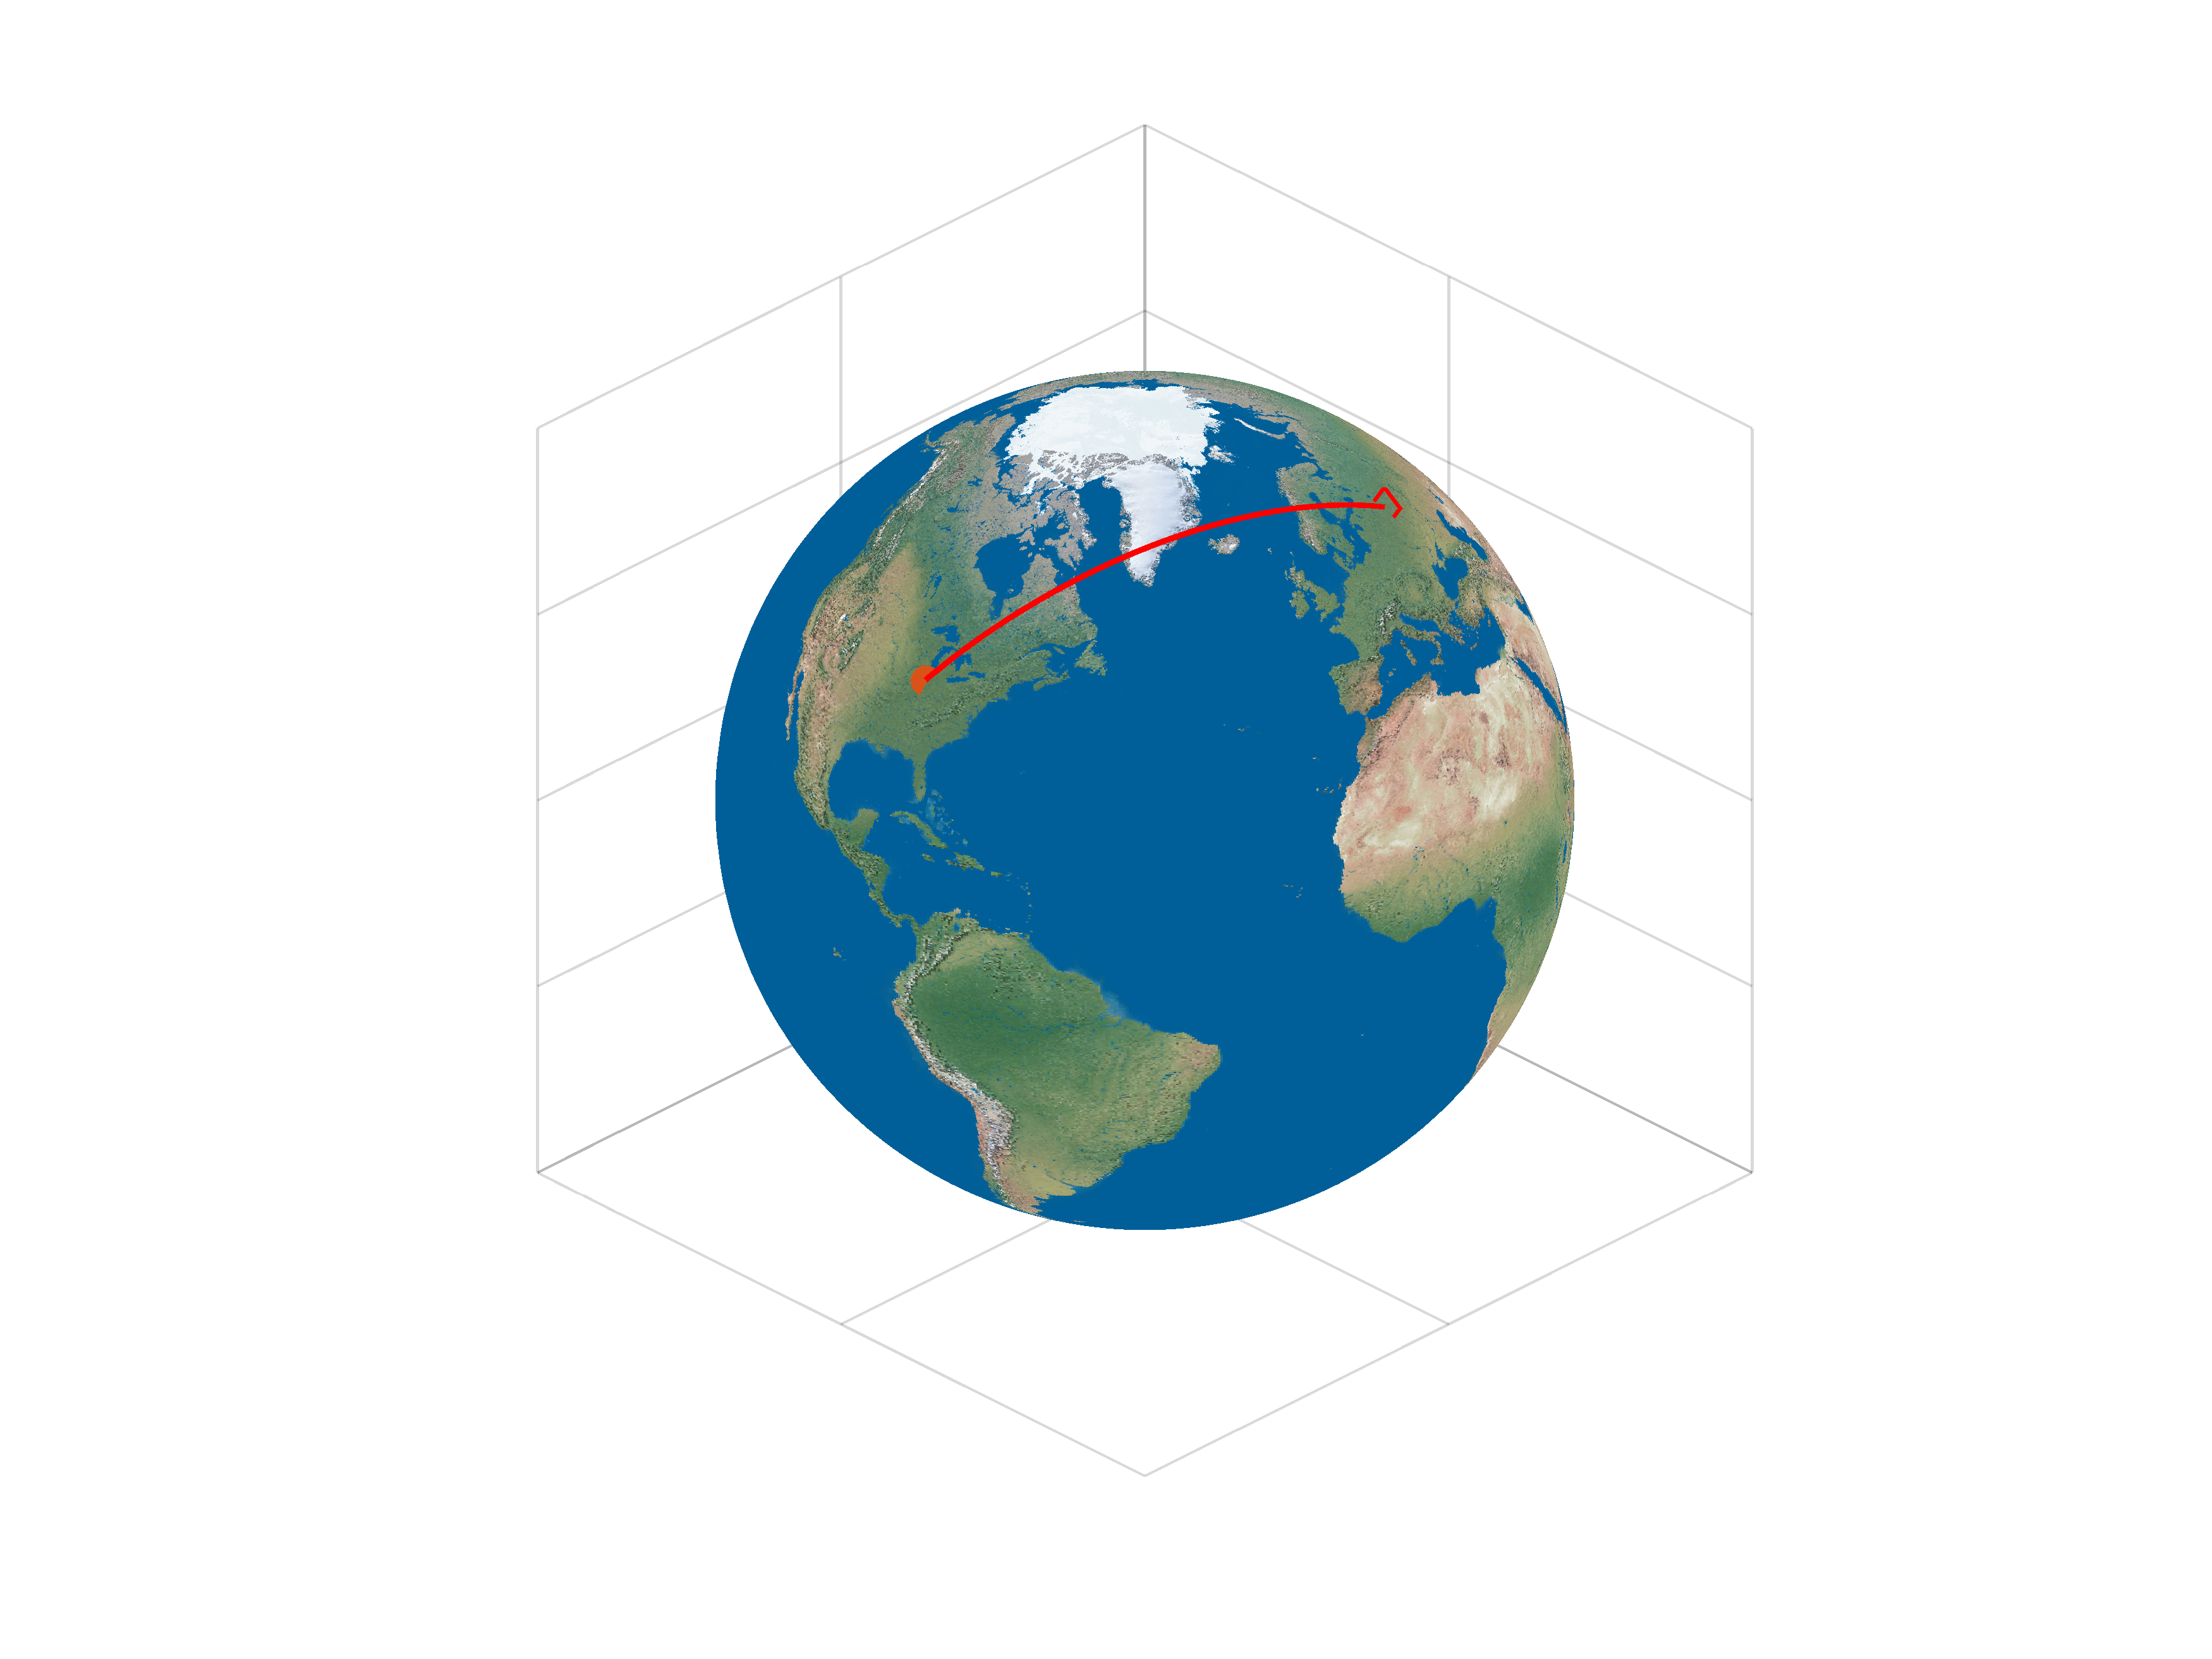
\includegraphics[width=.75\linewidth]{Scripts/Geodesic.png}
    \caption{Geodesic shown on the Earth}
    \label{fig:Geodesic}
\end{figure}

For a short path length where the distance is much smaller than the sphere radius $r$, we expect that this will return the standard straight line as the shortest distance.

Performing a Taylor expansion and keeping only the first-order terms:
$$\frac{1}{\theta}=a$$
So, it is seen that the value $\theta$, as expected, is constant for a short path length. This formula thus returns the standard equation of a line on short scales!

One important consequence of this is that a spherical geometry, when looked at `closely' (this is, looking at an infinitesimal portion of the surface) is locally Euclidean! This fact that the geometry looks locally Euclidean will be important in our later discussions in \autoref{chap:lie theory}.
\end{example}
 
\subsection{Revisiting the Brachistochrone}

\begin{example}[Brachistochrone]\label{ex:brachistrochrone}
    Let us return to the example of the \gls{brachistochrone} to demonstrate the usefulness of the calculus of variations in solving  this problem. Of course, we have seen John

    %clean this up and explain
You are a prominent mathematician in the year 1696. Bernoulli proposes a problem to you to find a curve from a point $(x_0,y_0)$ to another point $\left(x_f,y_f\right)$. When a particle is placed on this path, it should be a faster path than any other path the particle could take down the slope under the influence of only gravity.

Find the velocity as a function of the distance from the initial height, $h$, for the particle using energy conservation.

Write a general expression for the amount of time it takes a particle to descent a path using an integral. \textit{Hint: you can write $t=\frac{ds}{v}$}.

Use the Euler-Lagrange equation to solve for the form of this curve (You may find the integral form useful!). Plot the result.
\end{example}

\chapter{Lagrangian Mechanics}\label{chap:lagrangian}

\color{red} This chapter needs a large amount of work still. Need to finish reading through Goldstein and include neccesary information from there. Include generalized forces, lagrangian multipliers, improve non-holonomic constraints, write the quantuam to lagrangian section, and write some good practice problems.

\color{black}

Energy methods of mechanics use the energy of a system to determine the \gls{eom} of the system . This is in contrast to the Newtonian method, which considers the forces of a system to produce its \gls{eom}. The good news is that both will result in the same answer (see proof in \autoref{equiv newt and lang}). However, having both in your set of tools as an engineer can prove especially useful.

To grasp energy methods, it is best to have an intuition for Newtonian dynamics first. A thorough reading of Volume I and other sources will help prepare the reader for this section. The two are quite different, but the \gls{Lagrangian} formalism deals less with intuition and more with analytical solutions, so having the intuition from the Newtonian approach will be useful.

There are two main types of energy mechanics, referred to as \gls{Hamiltonian} and \gls{Lagrangian} Mechanics. In this chapter, we will mostly focus on the \gls{Lagrangian} version of these mechanics. \gls{Hamiltonian} mechanics will be discussed further in \autoref{chap:hamiltonian}. Both approaches use energy, but have some distinct differences in implementation. Generally, the \gls{Lagrangian} approach is more suited to solving problems in classical dynamics, so we will start with this approach.

\newglossaryentry{symplectic int}
{
    name=symplectic integrator,
    first = {\textit{symplectic integrator}},
    description={A class of numerical integration schemes that are energy preserving because they preserve certain geometric properties of a differential equation}
}

Although the \gls{Hamiltonian} and \gls{Lagrangian} are not directly used in the case of our 6-\gls{dof}, they are fundamental to other areas of mechanics and make derivations far simpler in many cases. The \gls{Hamiltonian} and \gls{Lagrangian} descriptions of mechanics are more often taught to physics students rather than engineers, but we feel that they deserve inclusion among the topics presented here. For the reader interested in applications in robotics, energy mechanics has a vast number of applications.

When we discuss \gls{numerical int}, we can use \glspl{symplectic int} when our problem has a \gls{Hamiltonian} description. This will be further discussed in \autoref{sec: Syplectic Ints}. You may find that certain \gls{eom} derivations, such as the spinning top and problems in orbital mechanics are more easily accomplished with energy methods. Another reason to motivate these systems is that these energy methods are invariant to transformations such as rotations. This occurs because energy methods employ a generalized coordinate system. These generalized coordinates are very powerful and allow us to describe a huge variety of systems. We will see this later in some examples.

A brief overview of the differences between the two schemes of \gls{eom} derivation is shown in \autoref{fig:newt v lang}. As can be seen from the figure, the underlying governing mechanics are no different, but the way in which we arrive at the \gls{eom} is completely different. Knowing this, we can begin our dive into \gls{Lagrangian} mechanics.

\begin{figure}[ht]
    \centering
    
\includesvg[width=.6\linewidth]{Images/NewtonianLagrangian.svg}

    \caption{Newtonian vs. Lagrangian Mechanics Approach}
    \label{fig:newt v lang}
\end{figure}

\section{Hamilton's Principle}
The basis of \gls{Lagrangian} mechanics is Hamilton's Principle. Similar to Fermat's principle of least time, Hamilton's principle states that a quantity called the \gls{action} must be minimized.

Although we may not have a physical intuition of why this is true right now (that will come later), it proves to be especially useful. Additionally, these ideas follow direction from the calculus of variations! Hamilton (alongside some others) formulated a definition of this principle that describes all physical systems. Hamilton's Principle is as follows:
\begin{theorem}[Hamilton's Principle]
In a conservative system which may travel from one point to another within a specific time interval, the path that is followed is the path which minimizes the time integral of the difference between the kinetic and potential energies.
$$\delta \int_{t_1}^{t_2}{T-U}{dt}=0$$
\end{theorem}

The quantity $T-U$, the kinetic energy minus the potential energy, is a quantity called the \gls{Lagrangian}, denoted $L$. 
\begin{equation}
    L\equiv T-U
\end{equation}
The \gls{Lagrangian} typically has no physical meaning. Instead, we simply choose a \gls{Lagrangian} such that the laws of mechanics work. The reason for the negative sign on the potential, $U$, can be seen in the derivation in \autoref{equiv newt and lang}. In short, the negative must be present so that the \gls{Lagrangian} matches the Newtonian description.

Before we get too ahead of ourselves, though, we should investigate this integral a bit further. We can notice that the form of the integral is quite similar to the equations we have seen in the calculus of variations.

In fact, we can notice that the potential energy, generally, is a function of the position, $y$, and the kinetic energy is a function of $y'$ -- the time derivative of the position. As a result, we can write our \gls{Lagrangian} quite generally as:
$$\int_{t_1}^{t_2}f[y(x),y(x)';x]dx$$
This of course, matches the definition for the functional that we described in \autoref{chap:calculus of variations}.

\newglossaryentry{princ of least action}
{
    name=principle of least action,
    first = {\textit{principle of least action}},
    description={A form of Hamilton's Principle that states that the action of a system should be minimized in a physical mechanical system},
    see={action}
}
In the case of \gls{Lagrangian} mechanics, the functional is called the \gls{action}, denoted $S$. This is often why Hamilton's Principle is also called the \gls{princ of least action}.  We can thus equivalently write the integral as:
\begin{equation}
    S=\int_{t_1}^{t_2}{L}{dt}
\end{equation}
So, our \gls{action} takes the form of the \gls{functional} from the calculus of variations. From Hamilton's principle, this \gls{functional}, the \gls{action}, must be minimized. So, we often see the compact form of Hamilton's Principle as:
$$\delta S=0$$
We know from our previous studies that the extremal conditions of a functional can be found using the \gls{Euler Equation}.

\newglossaryentry{euler lagrange}
{
    name=Euler-Lagrange equation,
    first = {\textit{Euler-Lagrange equation}},
    description={The fundemental equation describing the solutions that give the extrema of the action in a Lagrangian system.},
    see={action}
}

Substituting in the variables that we use for the \gls{Lagrangian}, we have the \glspl{euler lagrange}, which is used to find the extremal solutions:
\begin{gather}\label{eq: Euler-Lagrange}
    \color{blue}\boxed{\color{black}\frac{\partial L}{\partial x_i}-\frac{d}{dt}\frac{\partial L}{\partial \dot{x}_i}=0}\\ \mathrm{\color{blue}Euler-Lagrange \ Equations}
\end{gather}
Hamilton's Principle then states that the solutions to this \gls{euler lagrange} are the \gls{eom} of the system!

There is one small part of the principle that I glossed over during the derivation; the fact that the system must be \gls{conservative}. In short, a \gls{conservative} system is one in which the energy of the particle is path-independent. See \cite{goldstein_classical_2008} Chapter 1 for more information. This assumption helped when I assumed that the potential, $U$, was a function of position only. If this potential had a dependence of velocity, then the problem would not be easily solvable.

This does mean that frictional forces and aerodynamics are not modeled with the \gls{Lagrangian} we describe here (although they can be with the utilization of Rayleigh's dissipation function and other techniques, such as those discussed in \cite{rabei_hamiltonian_2004}). This is the reason we do not directly use these equations in the 6-DoF.\footnote{However, much of the rotational dynamics we describe can be represented equivalently using the \gls{Lagrangian} approach, so we do use these equations in a roundabout manner.} This is also one reason that we need to use numerical integration methods to solve the \gls{eom} for the rocket trajectory when using Newtonian dynamics. In fact, the idea that the system in non-\gls{conservative} and cannot be solved analytically are intrinsically linked.

So, for systems that are non-conservative, it is best to stick with the Newtonian method of mechanics, as we do for our 6-DoF, since the methods to find approximate solutions for these equations are quite a bit simpler. 

However, for systems that are frictionless, the methods described here will work well. While it may seem that frictionless systems are very idealistic, we do see systems that can be approximated as frictionless quite often! Orbits, of course, are one case where this is especially true. For many other systems, such as a spinning top or other rotating bodies, we can often ignore the small amount of friction and arrive at analytical solutions without much hassle using the \gls{Lagrangian}. These methods also become extraordinarily important for our derivations of rotational equations.

I should also note that the concept of friction and air drag is only a macroscopic one. All of the interactions that we regard as friction are fundamentally electromagnetic in origin. Therefore, in fundamental and theoretical physics, the energy methods of mechanics are almost always suitable methods! Unfortunately, our 6-\gls{dof} model does not simulate atomic interactions, so us engineers are sometimes stuck with the barbaric methods of Newton.

With that noted, let us use the \gls{Lagrangian} in a few examples to see how it can turn some complex Newtonian systems into fairly trivial problems.
\subsection{Mass-Spring System}
As a very basic prototypical system, we will consider a mass spring system as shown in \autoref{fig:mass spring lagrange}. We consider the length $x$ to be referenced from the rest length of the spring.
\begin{figure}[ht]

\centering

\tikzset{every picture/.style={line width=0.75pt}} %set default line width to 0.75pt        

\begin{tikzpicture}[x=0.75pt,y=0.75pt,yscale=-1,xscale=1]
%uncomment if require: \path (0,300); %set diagram left start at 0, and has height of 300

%Rounded Rect [id:dp34438430167397516] 
\draw  [color={rgb, 255:red, 0; green, 0; blue, 0 }  ,draw opacity=1 ][fill={rgb, 255:red, 255; green, 255; blue, 255 }  ,fill opacity=1 ] (310,154) .. controls (310,140.75) and (320.75,130) .. (334,130) -- (406,130) .. controls (419.25,130) and (430,140.75) .. (430,154) -- (430,226) .. controls (430,239.25) and (419.25,250) .. (406,250) -- (334,250) .. controls (320.75,250) and (310,239.25) .. (310,226) -- cycle ;
%Straight Lines [id:da2744613466135113] 
\draw    (110,250) -- (110,212) ;
\draw [shift={(110,210)}, rotate = 90] [color={rgb, 255:red, 0; green, 0; blue, 0 }  ][line width=0.75]    (7.65,-2.3) .. controls (4.86,-0.97) and (2.31,-0.21) .. (0,0) .. controls (2.31,0.21) and (4.86,0.98) .. (7.65,2.3)   ;
%Straight Lines [id:da08431663295207847] 
\draw    (110,250) -- (148,250) ;
\draw [shift={(150,250)}, rotate = 180] [color={rgb, 255:red, 0; green, 0; blue, 0 }  ][line width=0.75]    (7.65,-2.3) .. controls (4.86,-0.97) and (2.31,-0.21) .. (0,0) .. controls (2.31,0.21) and (4.86,0.98) .. (7.65,2.3)   ;
%Shape: Spring [id:dp2050444045141704] 
\draw   (200,190) .. controls (201.25,180) and (205.25,170) .. (213.25,170) .. controls (229.25,170) and (229.25,210) .. (223.25,210) .. controls (217.25,210) and (217.25,170) .. (233.25,170) .. controls (249.25,170) and (249.25,210) .. (243.25,210) .. controls (237.25,210) and (237.25,170) .. (253.25,170) .. controls (269.25,170) and (269.25,210) .. (263.25,210) .. controls (257.25,210) and (257.25,170) .. (273.25,170) .. controls (289.25,170) and (289.25,210) .. (283.25,210) .. controls (277.25,210) and (277.25,170) .. (293.25,170) .. controls (309.25,170) and (309.25,210) .. (303.25,210) .. controls (297.69,210) and (297.28,175.62) .. (310,170.61) ;
%Straight Lines [id:da8109677911849542] 
\draw [line width=1.5]    (200,250) -- (500,250) ;
%Straight Lines [id:da9738860715008741] 
\draw [line width=1.5]    (200,130) -- (200,250) ;
%Straight Lines [id:da8479892294914445] 
\draw [color={rgb, 255:red, 74; green, 144; blue, 226 }  ,draw opacity=1 ]   (290,110) -- (368,110) ;
\draw [shift={(370,110)}, rotate = 180] [color={rgb, 255:red, 74; green, 144; blue, 226 }  ,draw opacity=1 ][line width=0.75]    (10.93,-3.29) .. controls (6.95,-1.4) and (3.31,-0.3) .. (0,0) .. controls (3.31,0.3) and (6.95,1.4) .. (10.93,3.29)   ;
\draw [shift={(290,110)}, rotate = 180] [color={rgb, 255:red, 74; green, 144; blue, 226 }  ,draw opacity=1 ][line width=0.75]    (0,5.59) -- (0,-5.59)   ;
%Straight Lines [id:da38778280879589844] 
\draw    (200,260) -- (210,250) ;
%Straight Lines [id:da13716831040628819] 
\draw    (220,260) -- (230,250) ;
%Straight Lines [id:da5435450145291132] 
\draw    (240,260) -- (250,250) ;
%Straight Lines [id:da6012450156738026] 
\draw    (260,260) -- (270,250) ;
%Straight Lines [id:da006204164316379712] 
\draw    (280,260) -- (290,250) ;
%Straight Lines [id:da6672054023307342] 
\draw    (300,260) -- (310,250) ;
%Straight Lines [id:da05532576658672206] 
\draw    (320,260) -- (330,250) ;
%Straight Lines [id:da713074642825677] 
\draw    (340,260) -- (350,250) ;
%Straight Lines [id:da054951797337481234] 
\draw    (360,260) -- (370,250) ;
%Straight Lines [id:da44290965384713543] 
\draw    (380,260) -- (390,250) ;
%Straight Lines [id:da1554621606788551] 
\draw    (400,260) -- (410,250) ;
%Straight Lines [id:da18496092525096441] 
\draw    (420,260) -- (430,250) ;
%Straight Lines [id:da9097830383289192] 
\draw    (440,260) -- (450,250) ;
%Straight Lines [id:da2668563479968923] 
\draw    (460,260) -- (470,250) ;
%Straight Lines [id:da6488797889553993] 
\draw    (480,260) -- (490,250) ;
%Straight Lines [id:da8070575578091496] 
\draw    (190,150) -- (200,140) ;
%Straight Lines [id:da3401604231163561] 
\draw    (190,170) -- (200,160) ;
%Straight Lines [id:da12031548793524682] 
\draw    (190,190) -- (200,180) ;
%Straight Lines [id:da3325006766252374] 
\draw    (190,210) -- (200,200) ;
%Straight Lines [id:da6789154128761035] 
\draw    (190,230) -- (200,220) ;
%Straight Lines [id:da23421921174832838] 
\draw    (190,250) -- (200,240) ;

% Text Node
\draw (151,238.4) node [anchor=north west][inner sep=0.75pt]    {$\hat{x}$};
% Text Node
\draw (107,186.4) node [anchor=north west][inner sep=0.75pt]    {$\hat{y}$};
% Text Node
\draw (327,90) node  [color={rgb, 255:red, 74; green, 144; blue, 226 }  ,opacity=1 ]  {$x$};

\end{tikzpicture}

    \caption{Mass-Spring System for Lagrangian}
    \label{fig:mass spring lagrange}
\end{figure}

We know the analytical form of the \gls{eom} from Newtonian Dynamics:
$$m\ddot{x}+kx=0$$
So, in essence, we are using the \gls{Lagrangian} \textit{a posteriori} to match this solution.

First, we will find the \gls{Lagrangian} of the system. The kinetic energy of the particle is given by the linear translation only (there is no rotational motion for a point particle), so we have $T=\frac{1}{2}m\dot{x}^2$. The potential energy is the energy of the spring, given as $U=\frac{1}{2}kx^2$. So, the \gls{Lagrangian} is:
$$L=\frac{1}{2}m\dot{x}^2-\frac{1}{2}kx^2$$
Now, applying \eqautoref{eq: Euler-Lagrange} in the $\hat{x}$-direction, as this is the only degree of freedom:
$$\frac{\partial L}{\partial x}-\frac{d}{dt}\frac{\partial L}{\partial \dot{x}}=0$$
Taking each term individually,
$$\frac{\partial L}{\partial x}=-kx$$
$$\frac{\partial L}{\partial \dot{x}}=m\dot{x}$$
$$\frac{d}{dt}\left(m\dot{x}\right)=m\ddot{x}$$
So, the \eqautoref{eq: Euler-Lagrange} equation gives us:
$$-kx-m\ddot{x}=0$$
A simple change of signs gives the exact same result as the Newtonian approach:
$$m\ddot{x}+kx=0$$
In this problem, we used a simple case where the dynamics were constrained along a single axis of motion. Before we move to a more complex problem, we will introduce the method by which \gls{Lagrangian} mechanics deals with these reference frames.
\section{Generalized Coordinates}
\color{red} Need to possibly reorganize some of this. Should explain why generalized coordinates are needed in the context of constraints and how they solve problems with coordinates being coupled.

\color{black}

We recall that in Newtonian mechanics, we describe reference frames for an object. We represent the position, velocity, and acceleration of a particle in terms of these coordinate systems as a tridimensional vector. 
Generally, we may write the $\vec{r}^{\ op}$  vector in a frame $a$ as:
$$x\hat{a}_1+y\hat{a}_2+z\hat{a}_3$$
Because any tridimensional set of coordinates that we choose that are linearly independent of each other will span $\mathbb{R}^3$, we can generalize this to any reference frame, $q$, where the terms of $a$ can be described by the terms of $q$:
$$x\left(q_1,q_2,q_3\right)+y\left(q_1,q_2,q_3\right)+z\left(q_1,q_2,q_3\right)$$
As a shorthand, we will write this full set of $q$, $\left(q_1,q_2,\cdots q_n\right)$, as $q_j$.

We can also generalize this to the velocity and the acceleration. The components of velocity can be written in terms of $q_j, \dot{q}_j$ and those for acceleration in terms of $q_j, \dot{q}_j, \ddot{q}_j$.  When we do Newtonian dynamics, we need to use the \gls{bke} to transform these quantities if they are not in an \gls{inertial frame}. Not so with the \gls{Lagrangian}! We are free to choose whatever $q$'s we want.

For a single particle, we can describe its position with the $q_j$ coordinates. When multiple particles are involved, we may need to increase this number of $q$ coordinates. As a very general statement, we can say for $N$ particles, we will need $n$ generalized coordinates in $q$. Expressed vectorially, given a particle of the $i^{\mathrm{th}}$ index:
$$\vec{r}^{\ oi}(q_j)$$
In other words, the position of an arbitrary particle is given in terms of $n$ generalized coordinates. 

The acceleration of the particles, when Newton's Laws are applied, are a function of the $q_j$ as well as their derivatives, $\dot{q}_j$. So, the evolution of the system exists in a $2n$-dimensional state space. However, we can use our previously mentioned \gls{Lagrangian} to circumvent the need for Newton's Law and the \gls{bke} in our derivation of the \gls{eom} using \textit{constraints} on the equation.

\subsection{Constraints}\label{sec:constaints}
Constraint equations are fundamental to \gls{Lagrangian} mechanics. In the previous section, I stated the need for $n$ generalized coordinates. To find a precise number for a given system, we turn our attention to constraints.

We can imagine constraints as a condition that restricts the motion of a body in some way. A body which has complete freedom to move translationally and rotate in any way is free. When a constraint is applied, this freedom is reduced. Often, we see these constraints denoted with either an equality or an inequality. These constraints, most often, are functions of the position, velocity, and/or time. We see constraints written most often in the form:
$$f(\vec{r},\vec{v},t)=0$$
The powerful thing about constraints in \gls{Lagrangian} mechanics is that we only need to know the way in which a particle is constrained, not the force or analytical description of this constraint. For complex problems, this can be especially useful.

\subsubsection{Holonomic Constraints}

To contextualize this, we take the example of a system of $N$ particles. For each particle, we need 3 values to define the position, so we need $3N$ generalized coordinates. 

\newglossaryentry{holonomic const}
{
    name=holonomic constraint,
    first = {\textit{holonomic constraint}},
    description={A constraint on a Lagrangian system which is a function of only the position of the particles},
    see={Lagrangian}
}

However, we often have constraints that reduce this number. Often, we see a problem that is planar or where the particles are connected in a \gls{rigid body}. These constraints will reduce the number of generalized coordinates needed. Here, we are only considering constraints on the positions of particles. Constraints on the positions of particles are known as \glspl{holonomic const}. 

A \gls{holonomic const} relates generalized coordinates to each other. In the commonly used notation, the \gls{holonomic const} is expressed in terms of the $q_j$'s as:
$$\Phi_k\left(q_j,t\right)=0, \ k=1\cdots K$$
or in terms of the position vectors:
$$f_k\left(\vec{r}^{\ op_1},\vec{r}^{\ op_2}\cdots \vec{r}^{\ op_N},t\right)=0$$
The number of \glspl{holonomic const}, $K$, will change the number of generalized coordinates as:
\begin{gather}\label{eq:dof}
\color{blue}\boxed{\color{black}\mathcal{M}=3N-K}\color{black}
\end{gather}
The quantity $\mathcal{M}$ is the number of \gls{dof}. However, this is the number of \gls{dof} for the whole system, which is why it can exceed 6 in some cases!

   \begin{example}[Particle on Path]
        Suppose we have a single particle that is constrained to motion along a path in the $xy$-plane. This path is given by $y=g(x)$. 
\begin{figure}[H]
    \centering



\tikzset{every picture/.style={line width=0.75pt}} %set default line width to 0.75pt        

\begin{tikzpicture}[x=0.75pt,y=0.75pt,yscale=-1,xscale=1]
%uncomment if require: \path (0,300); %set diagram left start at 0, and has height of 300

%Straight Lines [id:da4836354473889902] 
\draw    (280,200) -- (280,52) ;
\draw [shift={(280,50)}, rotate = 90] [color={rgb, 255:red, 0; green, 0; blue, 0 }  ][line width=0.75]    (7.65,-2.3) .. controls (4.86,-0.97) and (2.31,-0.21) .. (0,0) .. controls (2.31,0.21) and (4.86,0.98) .. (7.65,2.3)   ;
%Straight Lines [id:da02796272069122141] 
\draw    (280,200) -- (428,200) ;
\draw [shift={(430,200)}, rotate = 180] [color={rgb, 255:red, 0; green, 0; blue, 0 }  ][line width=0.75]    (7.65,-2.3) .. controls (4.86,-0.97) and (2.31,-0.21) .. (0,0) .. controls (2.31,0.21) and (4.86,0.98) .. (7.65,2.3)   ;
%Straight Lines [id:da7509100626039666] 
\draw    (280,200) -- (221.41,258.59) ;
\draw [shift={(220,260)}, rotate = 315] [color={rgb, 255:red, 0; green, 0; blue, 0 }  ][line width=0.75]    (7.65,-2.3) .. controls (4.86,-0.97) and (2.31,-0.21) .. (0,0) .. controls (2.31,0.21) and (4.86,0.98) .. (7.65,2.3)   ;
%Curve Lines [id:da26997678379551215] 
\draw [color={rgb, 255:red, 74; green, 144; blue, 226 }  ,draw opacity=1 ]   (210,180) .. controls (290.81,63.46) and (321.48,207.46) .. (410,90) ;
%Straight Lines [id:da09225730190804848] 
\draw [color={rgb, 255:red, 208; green, 2; blue, 27 }  ,draw opacity=1 ]   (280,200) -- (338.59,141.41) ;
\draw [shift={(340,140)}, rotate = 135] [color={rgb, 255:red, 208; green, 2; blue, 27 }  ,draw opacity=1 ][line width=0.75]    (10.93,-3.29) .. controls (6.95,-1.4) and (3.31,-0.3) .. (0,0) .. controls (3.31,0.3) and (6.95,1.4) .. (10.93,3.29)   ;
\draw [shift={(280,200)}, rotate = 315] [color={rgb, 255:red, 208; green, 2; blue, 27 }  ,draw opacity=1 ][fill={rgb, 255:red, 208; green, 2; blue, 27 }  ,fill opacity=1 ][line width=0.75]      (0, 0) circle [x radius= 3.35, y radius= 3.35]   ;
%Shape: Circle [id:dp7406066990608903] 
\draw  [fill={rgb, 255:red, 0; green, 0; blue, 0 }  ,fill opacity=1 ] (338.33,140) .. controls (338.33,139.08) and (339.08,138.33) .. (340,138.33) .. controls (340.92,138.33) and (341.67,139.08) .. (341.67,140) .. controls (341.67,140.92) and (340.92,141.67) .. (340,141.67) .. controls (339.08,141.67) and (338.33,140.92) .. (338.33,140) -- cycle ;

% Text Node
\draw (433,190.4) node [anchor=north west][inner sep=0.75pt]    {$x$};
% Text Node
\draw (277,22.4) node [anchor=north west][inner sep=0.75pt]    {$y$};
% Text Node
\draw (209,256.4) node [anchor=north west][inner sep=0.75pt]    {$z$};
% Text Node
\draw (282,203.4) node [anchor=north west][inner sep=0.75pt]    {$O$};
% Text Node
\draw (337,112.4) node [anchor=north west][inner sep=0.75pt]    {$P$};
% Text Node
\draw (420,72.4) node [anchor=north west][inner sep=0.75pt]  [color={rgb, 255:red, 74; green, 144; blue, 226 }  ,opacity=1 ]  {$y=g( x)$};
% Text Node
\draw (321,162.4) node [anchor=north west][inner sep=0.75pt]  [color={rgb, 255:red, 208; green, 2; blue, 27 }  ,opacity=1 ]  {$\vec{r}^{\ op}$};

\end{tikzpicture}

    \caption{Particle Moving on Constrained Path}
    \label{fig:constrainted path}
\end{figure}
We can select our generalized coordinates to be the same as the cartesian coordinates, so that:
\begin{gather}
    q_1=x\\q_2=y\\q_3=z
\end{gather}
With no other information, this is likely the best choice of generalized coordinates. However, we can start applying the constraints to simplify the equation. The first constraint is that the motion is confined to the $xy$-plane. Thus, 
$$q_3=z=0$$
Next, we have the path constraint which is given by $y=g(x)$. We can write this as a \glspl{holonomic const}:
\begin{gather}
    q_2-g(x)=0
\end{gather}
With these two constraints, we have reduced the number of degrees of freedom, $\mathcal{M}$, to 1. This makes sense intuitively, as the particle can only move along the path specified by the equation $g(x)$, therefore only having one degree of freedom.

In this example, we could describe that single degree of freedom with our coordinate, $q_1=x$.

The power of using generalized coordinates is that we could choose a coordinate that more easily defines this system. For example, our one coordinate could be the arc length along the path, $s$ defined from some starting point.
\end{example}

In general, these generalized coordinates do not even need to have units of length! We can select any parameters that are most convenient for defining the state, even those that are energies or fourier coefficients, so long as we can define a continuous derivative of that state and use the \gls{euler lagrange}.

\subsubsection{Rigid Body Constraints}\label{sec: rigid body constraints}
For most of the systems that we will deal with, including our rocket, we make the assumption that particles are rigidly attached to each other, meaning that there is no change in distance between particles. Using the notation of constraints described above, we will show how this is done for a two particle system, which can then naturally be extended with more particles.

Given two particles that are connected together by a massless rigid rod of length L, we have a constraint on the particles distance:
$$\left\Vert \vec{r}^{\ op_1}-\vec{r}^{\ op_2}\right\Vert=L$$
Written in the more standard notation:
$$f\left(\vec{r}^{\ op_1},\vec{r}^{\ op_2}\right)=\left\Vert \vec{r}^{\ op_1}-\vec{r}^{\ op_2}\right\Vert-L=0$$
So this constraint takes the 6-\gls{dof} for the two particles and reduces it to 5-\gls{dof}.

An example of the generalized coordinates describing this system would be the position of the first particle in Cartesian coordinates (giving 3 of the generalized coordinates, $x,y,z$, and the azimuthal and elevation angle, $\phi$ and $\theta$. The roll angle does not change the system in any measurable way, hence we only need 5 parameters to define a two particle system.

In the general case of $N$ particles composing a \gls{rigid body}, we have $3N$-\gls{dof} in a completely unconstrained system. However, we must constrain each pair of particles. An example of this for the 3 particle system in shown in \autoref{fig:rigid body 3 particle}.

\begin{figure}[ht]
    \centering
 

\tikzset{every picture/.style={line width=0.75pt}} %set default line width to 0.75pt        

\begin{tikzpicture}[x=0.75pt,y=0.75pt,yscale=-1,xscale=1]
%uncomment if require: \path (0,300); %set diagram left start at 0, and has height of 300

%Shape: Circle [id:dp11919774335444377] 
\draw  [fill={rgb, 255:red, 74; green, 144; blue, 226 }  ,fill opacity=0.59 ] (120,135) .. controls (120,121.19) and (131.19,110) .. (145,110) .. controls (158.81,110) and (170,121.19) .. (170,135) .. controls (170,148.81) and (158.81,160) .. (145,160) .. controls (131.19,160) and (120,148.81) .. (120,135) -- cycle ;
%Shape: Circle [id:dp1512759538865308] 
\draw  [fill={rgb, 255:red, 74; green, 144; blue, 226 }  ,fill opacity=0.59 ] (360,235) .. controls (360,221.19) and (371.19,210) .. (385,210) .. controls (398.81,210) and (410,221.19) .. (410,235) .. controls (410,248.81) and (398.81,260) .. (385,260) .. controls (371.19,260) and (360,248.81) .. (360,235) -- cycle ;
%Shape: Circle [id:dp4443678325062712] 
\draw  [fill={rgb, 255:red, 74; green, 144; blue, 226 }  ,fill opacity=0.59 ] (380,65) .. controls (380,51.19) and (391.19,40) .. (405,40) .. controls (418.81,40) and (430,51.19) .. (430,65) .. controls (430,78.81) and (418.81,90) .. (405,90) .. controls (391.19,90) and (380,78.81) .. (380,65) -- cycle ;
%Straight Lines [id:da963502184755707] 
\draw    (170,130) -- (380,70) ;
%Straight Lines [id:da5114822387415651] 
\draw    (167.27,146.68) -- (361.67,226.68) ;
%Straight Lines [id:da3674207943033927] 
\draw    (405,90) -- (389.67,209.88) ;

% Text Node
\draw (145,135) node    {$m_{1}$};
% Text Node
\draw (385,235) node    {$m_{3}$};
% Text Node
\draw (405,65) node    {$m_{2}$};
% Text Node
\draw (91,125.4) node [anchor=north west][inner sep=0.75pt]    {$\vec{r}_{1}$};
% Text Node
\draw (421,242.4) node [anchor=north west][inner sep=0.75pt]    {$\vec{r}_{3}$};
% Text Node
\draw (351,25.4) node [anchor=north west][inner sep=0.75pt]    {$\vec{r}_{2}$};
% Text Node
\draw (229,65.4) node [anchor=north west][inner sep=0.75pt]    {$|\vec{r}_{1} -\vec{r}_{2} |$};
% Text Node
\draw (215.4,202.2) node [anchor=north west][inner sep=0.75pt]    {$|\vec{r}_{1} -\vec{r}_{3} |$};
% Text Node
\draw (402.6,136.6) node [anchor=north west][inner sep=0.75pt]    {$|\vec{r}_{2} -\vec{r}_{3} |$};

\end{tikzpicture}

    \caption{3 Particle Rigid Body}
    \label{fig:rigid body 3 particle}
\end{figure}

So, we have 3 constraint equations in a system with 9 particles. This gives a total of $3N-3=6$-\gls{dof}. When any additional particles are added, they must be fully constrained in all 3 translational degrees of freedom by constraints between $r_1$,$r_2$, and $r_3$. So, we always have constraints of the form $3N-3(N-2)$ for a \gls{rigid body}. This is why we always see a \gls{rigid body} displaying 6-\gls{dof}. We can then, of course, parametrize this in general coordinates with the cartesian coordinates and 3 angles.

\subsubsection{Minimal Set of Constraints}

\newglossaryentry{holonomic sys}
{
    name=holonomic system,
    first = {\textit{holonomic system}},
    description={A system that is entirely composed of holonomic constraints},
    see={holonomic const}
}
So far, we have only discussed holonomic constraints, those that are related to position or on the generalized parameters, and possibly have some relation in time. When a system is a \gls{holonomic sys}, that is, purely defined by \glspl{holonomic const}, it is always possible to find a set of $\mathcal{M}$ generalized parameters to describe the particle motion. In other words, the minimum number of parameters is equivalent to the number of degrees of freedom in the system.

That said, we often choose to use more parameters, particularly in the case of rotations. As we see in Volume II, we often find it more useful to use a non-minimal set of constraints to encode rotations to avoid singularities in the solution.

It is also common to see a non-minimal set of constraints used when the minimal set is cumbersome and does not give an intuitive feel to the problem. There is no strict requirement to use the minimal set of constraints for a problem, but you should be aware of the number of parameters required to describe the minimal set.
\subsubsection{Non-Holonomic Constraints}

\color{red} Discuss non integrability of non-holonomic constraints and the case of the rolling ball / ice skate.

\color{black}

\newglossaryentry{non holo const}
{
    name=non-holonomic constraint,
    first = {\textit{non-holonomic constraint}},
    description={A constraint that depends on more than the position of the particles in the system},
    see={holonomic const}
}
The other class of constraints are those constraints that are not merely a function of the generalized coordinates. These constraints, called \glspl{non holo const}, define the set of all constraints that depend on more than just the position of particles. This is a huge class of constraints, so we only cover specific cases here.

\newglossaryentry{gen vel}
{
    name=generalized velocity,
    first = {\textit{generalized velocity}},
    plural = {generalized velocities},
    firstplural = {\textit{generalized velocities}},
    description={A free direction of movement for a vehicle. These can be translational or rotational directions}
}

The most common among these, and where we will focus our attention here, is constraints on the time derivative of the generalized coordinates. These are called \glspl{gen vel}, denoted $\dot{q}_j$. Such an example of a constraint on \glspl{gen vel} is a roller skate. A roller stake only allows a velocity in the direction of the skate and restricts velocity along the direction normal to the roller stake.

One important thing about \glspl{non holo const} is that they do not reduce the number of parameters needed to define the system. Additionally, there is no general way to solve systems which have non-holonomic constraints. Later, we will look at a few cases which can be solved. For now, we will concern ourselves mostly with systems consisting of holonomic constraints.

It may seem that this limits us greatly, but in fact, this is not the case for most physics problems! When we are considering large systems, this may be quite limiting, but when considering small scale physics, such as atomic problems, we often find that \glspl{non holo const} are the exception, not the rule. Most systems are conservative and have constraints only on positions. As such, most of our modern theories can use these \glspl{Lagrangian}.

In the context of engineering problems, we can sometimes make derivations under the assumption of holonomic constraints and then use empirical data and correlations where needed to find suitable solutions (when friction or other factors are present).

\subsection{Lagrange's Equation in Generalized Coordinates}

The good thing about the \gls{Lagrangian} method is that it is invariant to changes in our coordinate system. Because the \gls{Lagrangian} is an equation of energy, and energy is independent of coordinate transformations, we can easily express the \gls{euler lagrange} in generalized coordinates with little hassle.\endnote{I note here that this explanation is not strictly correct, since our \gls{Lagrangian} does not have to be coordinate lengths. Instead, the configuration space has special properties that make it invariant to such transformations. Deriving the \gls{Lagrangian} from Hamilton's principle ensures that this is always true, which the intrepid reader may prove to themselves by studying differential geometry and Lagrangians on manifolds. Further information will be provided in \autoref{chap:lie theory} although we will not strictly cover this.} 

Using the generalized coordinates, the kinetic energy is a function of the generalized positions, velocities, and time. The potential is a function of the generalized position and time, so the \gls{Lagrangian} becomes:
$$L\equiv T-U=T(q_j,\dot{q}_j,t)-U(q_j,t)$$
Stated another way, the \gls{Lagrangian} is a function of the generalized positions, velocities, and time, as $L=L(q_j,\dot{q}_j,t)$. The \gls{euler lagrange} then becomes:
\begin{gather}\label{eq:Euler-Lagrange General}
\color{blue}\boxed{\color{black}\frac{\partial L}{\partial q_j}-\frac{d}{dt}\frac{\partial L}{\partial \dot{q}_j}=0,\quad j=1,2,\cdots M}\\
\mathrm{\color{blue}Generalized \ Euler-Lagrange \ Equations}
\end{gather}
Next we will show a problem where the rotational invariance and generalized coordinates proves especially useful in simplifying our derivation:
\section{Pendulum EOM Derivation}
\subsubsection{Problem Set-Up}
Suppose we have a pendulum of length L. The mass is rigidly attached to the pendulum. A reference frame $a$ that moves with the pendulum is shown in \autoref{fig:Pendulum}. The \gls{inertial frame} is also shown. The pendulum moves in only the $xy$ plane.
\begin{figure}[ht]

\centering

\tikzset{every picture/.style={line width=0.75pt}} %set default line width to 0.75pt        

\begin{tikzpicture}[x=0.75pt,y=0.75pt,yscale=-1,xscale=1]
%uncomment if require: \path (0,300); %set diagram left start at 0, and has height of 300

%Straight Lines [id:da8354203825727349] 
\draw    (320,60) -- (420,240) ;
\draw [shift={(320,60)}, rotate = 60.95] [color={rgb, 255:red, 0; green, 0; blue, 0 }  ][fill={rgb, 255:red, 0; green, 0; blue, 0 }  ][line width=0.75]      (0, 0) circle [x radius= 2.68, y radius= 2.68]   ;
%Shape: Arc [id:dp31284247913451657] 
\draw  [draw opacity=0] (403.12,208.97) .. controls (378.54,222.36) and (350.19,230) .. (320,230) -- (320,65) -- cycle ; \draw [color={rgb, 255:red, 74; green, 144; blue, 226 }  ,draw opacity=1 ]   (400.15,210.55) .. controls (376.27,222.96) and (348.98,230) .. (320,230) ; \draw [shift={(320,230)}, rotate = 357.91] [color={rgb, 255:red, 74; green, 144; blue, 226 }  ,draw opacity=1 ][line width=0.75]    (0,5.03) -- (0,-5.03)   ; \draw [shift={(403.12,208.97)}, rotate = 153.52] [fill={rgb, 255:red, 74; green, 144; blue, 226 }  ,fill opacity=1 ][line width=0.08]  [draw opacity=0] (8.04,-3.86) -- (0,0) -- (8.04,3.86) -- cycle    ;
%Shape: Circle [id:dp5099783674397224] 
\draw  [color={rgb, 255:red, 0; green, 0; blue, 0 }  ,draw opacity=1 ][fill={rgb, 255:red, 74; green, 74; blue, 74 }  ,fill opacity=1 ] (410,240) .. controls (410,234.48) and (414.48,230) .. (420,230) .. controls (425.52,230) and (430,234.48) .. (430,240) .. controls (430,245.52) and (425.52,250) .. (420,250) .. controls (414.48,250) and (410,245.52) .. (410,240) -- cycle ;
%Straight Lines [id:da8713569921261672] 
\draw [color={rgb, 255:red, 208; green, 2; blue, 27 }  ,draw opacity=1 ]   (340,50) -- (438.54,227.38) ;
\draw [shift={(440,230)}, rotate = 240.95] [fill={rgb, 255:red, 208; green, 2; blue, 27 }  ,fill opacity=1 ][line width=0.08]  [draw opacity=0] (8.93,-4.29) -- (0,0) -- (8.93,4.29) -- cycle    ;
\draw [shift={(340,50)}, rotate = 240.95] [color={rgb, 255:red, 208; green, 2; blue, 27 }  ,draw opacity=1 ][line width=0.75]    (0,5.59) -- (0,-5.59)   ;
%Straight Lines [id:da9538559670922312] 
\draw    (200,240) -- (200,202) ;
\draw [shift={(200,200)}, rotate = 90] [color={rgb, 255:red, 0; green, 0; blue, 0 }  ][line width=0.75]    (7.65,-2.3) .. controls (4.86,-0.97) and (2.31,-0.21) .. (0,0) .. controls (2.31,0.21) and (4.86,0.98) .. (7.65,2.3)   ;
%Straight Lines [id:da3275390122881038] 
\draw    (200,240) -- (238,240) ;
\draw [shift={(240,240)}, rotate = 180] [color={rgb, 255:red, 0; green, 0; blue, 0 }  ][line width=0.75]    (7.65,-2.3) .. controls (4.86,-0.97) and (2.31,-0.21) .. (0,0) .. controls (2.31,0.21) and (4.86,0.98) .. (7.65,2.3)   ;
%Straight Lines [id:da24072013587186947] 
\draw [color={rgb, 255:red, 208; green, 2; blue, 27 }  ,draw opacity=1 ]   (451.54,222.12) -- (470.54,255.03) ;
\draw [shift={(471.54,256.77)}, rotate = 240] [color={rgb, 255:red, 208; green, 2; blue, 27 }  ,draw opacity=1 ][line width=0.75]    (7.65,-2.3) .. controls (4.86,-0.97) and (2.31,-0.21) .. (0,0) .. controls (2.31,0.21) and (4.86,0.98) .. (7.65,2.3)   ;
%Straight Lines [id:da7099456662568205] 
\draw [color={rgb, 255:red, 208; green, 2; blue, 27 }  ,draw opacity=1 ]   (451.54,222.12) -- (484.45,203.12) ;
\draw [shift={(486.18,202.12)}, rotate = 150] [color={rgb, 255:red, 208; green, 2; blue, 27 }  ,draw opacity=1 ][line width=0.75]    (7.65,-2.3) .. controls (4.86,-0.97) and (2.31,-0.21) .. (0,0) .. controls (2.31,0.21) and (4.86,0.98) .. (7.65,2.3)   ;


% Text Node
\draw (362,227.4) node [anchor=north west][inner sep=0.75pt]  [color={rgb, 255:red, 74; green, 144; blue, 226 }  ,opacity=1 ]  {$\theta $};
% Text Node
\draw (391,122.4) node [anchor=north west][inner sep=0.75pt]  [color={rgb, 255:red, 208; green, 2; blue, 27 }  ,opacity=1 ]  {$L$};
% Text Node
\draw (241,228.4) node [anchor=north west][inner sep=0.75pt]    {$\hat{x}$};
% Text Node
\draw (197,176.4) node [anchor=north west][inner sep=0.75pt]    {$\hat{y}$};
% Text Node
\draw (481.25,191.58) node [anchor=north west][inner sep=0.75pt]  [color={rgb, 255:red, 208; green, 2; blue, 27 }  ,opacity=1 ,rotate=-330]  {$\hat{a}_{\theta }$};
% Text Node
\draw (467.54,261.84) node [anchor=north west][inner sep=0.75pt]  [color={rgb, 255:red, 208; green, 2; blue, 27 }  ,opacity=1 ,rotate=-330]  {$\hat{a}_{r}$};

\end{tikzpicture}

    \caption{Pendulum Set-Up}
    \label{fig:Pendulum}
\end{figure}
Our goal here is to approach the problem in several different ways to gain insight into the benefits and drawbacks of each method in a practical setting.

\subsubsection{Newtonian Approach}
You have likely seen the Newtonian approach many times, but we show it here for completeness and to contrast the approach with the \gls{Lagrangian} more directly. 

In the Newtonian Approach to deriving EOM's, we always start with the forces governing the system. In this case, we have two forces. The gravitational force, $mg$, acts in the $-\hat{y}$-direction and the tension force acts in the $-\hat{a}_r$-direction. From the constraint on length, the acceleration in the $\hat{a}_r$ must be zero. Thus, the component of gravity in the $\hat{a}_r$ direction must equal the tension.

We express the gravity in the $a$-frame to find this:
$$\hat{y}=-\cos\theta\hat{a}_r+\sin\theta \hat{a}_\theta$$
So, by balancing the forces in the $\hat{a}_r$-direction:
$$m{\ddot{a}}_r=mg\cos\theta \hat{a}_r-\vec{F}_T$$
In the $\hat{a}_\theta$-direction, we have unconstrained motion, so $\sum\vec{F}=m\vec{a}$. Our force equation is thus: 
$$F=-mg\sin\theta\hat{a}_{\theta}$$
Next, we need to find our acceleration in the \gls{inertial frame} using the \gls{bke} to solve the RHS of the force balance. Starting with the position vector:
$$\vec{r}^{\ op}=L\hat{a}_r$$
We can apply the \gls{bke} to find our inertial velocity:
$${}^i\vec{v}^p={}^a\frac{d}{dt}\vec{r}^{\ op}+{}^i\omega^a\times\vec{r}^{\ op}$$
Plugging in appropriate quantities:
$${}^i\vec{v}^p={}^a\frac{d}{dt}(L\hat{a}_r)+\dot{\theta}\hat{a}_3\times(L\hat{a}_r)$$
$${}^i\vec{v}^p=\dot{\theta}L\hat{a}_\theta$$
We do this again to find the inertial acceleration:
$${}^i\vec{a}^p={}^a\frac{d}{dt}{}^i\vec{v}^p+{}^i\omega^a\times{}^i\vec{v}^p$$
$${}^i\vec{a}^p={}^a\frac{d}{dt}{}\dot{\theta}L\hat{a}_\theta+\dot{\theta}\hat{a}_3\times\dot{\theta}L\hat{a}_\theta$$
$${}^i\vec{a}^p=\ddot{\theta}L\hat{a}_\theta-\dot{\theta}^2L\hat{a}_r$$
Now, we equate the forces in each direction:
$$-mg\sin\theta\hat{a}_\theta=\ddot{\theta}L\hat{a}_\theta$$
Rearranging, we arrive at our \gls{eom}:
$$\ddot{\theta}+\frac{g}{L}\sin\theta=0$$
\subsubsection{Lagrangian Approach}
In the \gls{Lagrangian} approach, we will start by defining our constraints and coordinates. Some preliminary analysis shows that using polar coordinates for this problem will be useful. If we do not recognize this, we can always convert later (a distinct advantage of the \gls{Lagrangian} approach, since it is coordinate frame invariant). Here we will choose a cylindrical coordinate systsem:
\begin{gather}
    q_1=r\\q_2=\theta\\q_3=z
\end{gather}
Next, we define constraints. Since there is no motion in the z-axis:
$$z=0$$
And the constraint on the length gives us:
$$q_1-L=0$$
So, we have 1 \gls{dof} from \eqautoref{eq:dof}. Since both $z$ and $r$ are constrained, we can express our \gls{eom} in terms of one generalized coordinate, $\theta$.

Next, we define the \gls{Lagrangian}. Knowing that the linear velocity of the particle is $\dot{\theta}L$, we get:
$$T=\frac{1}{2}m\dot{\theta}^2L^2$$
For the potential, we choose the origin as our reference, giving us:
$$U=-mgy$$
And a coordinate transformation into polar using $y=r\cos\theta$ yields:
$$U=-mgL\cos\theta$$
This gives the \gls{Lagrangian}:
$$L=\frac{1}{2}m\dot{\theta}^2L^2+mgL\cos\theta$$
Applying the Euler-Lagrange formula for generalized coordinates, \eqautoref{eq:Euler-Lagrange General} on the single generalized coordinate:
\begin{gather}
    \frac{\partial L}{\partial \theta}=-mgL\sin\theta\\
    \frac{\partial L}{\partial \dot{\theta}}=mL^2\dot{\theta}\\
    \frac{d}{dt}\left(mL^2\dot{\theta}\right)=mL^2\ddot{\theta}
\end{gather}
So, the final system is:
$$-mgL\cos\theta -mL^2\ddot{\theta}=0$$
With some rearrangement:
$$\ddot{\theta}+\frac{g}{L}\sin\theta=0$$
We notice that with the \gls{Lagrangian} approach, we did not need to have an understanding of the vector directions, frame translations, or \gls{bke} to find our \gls{eom}. This, in addition to the flexibility of the generalized coordinates, is the real power of this approach.

\subsubsection{Kinetic Energy Generalization}
In the previous two examples that we explored, the functions for $T$ and $U$ were quite simple because the transformations from the generalized coordinates were quite simple and could be understood from intuition. In the case that they are not as simple, we would previously have to use \gls{bke} to find transformations or employ some other method. It would be useful if we had a general formula to express $T$ and $U$ in the generalized coordinates. We know that the kinetic energy is simply the following:
$$T=\frac{1}{2}\sum_im_i{v_i}^2$$
We can more explicitly define $v_i$ to be $\dot{r}_i$, with $r$ being the vector in cartesian coordinates. The kinetic energy in terms of $\dot{r}$ is thus:
$$T=\frac{1}{2}\sum_im_i(\dot{r}_i\cdot\dot{r}_i)$$
As we have shown before, $r_i$ can generally be represented in terms of the generalized positions, $q_j$:
$$r_i=r_i(q_j)$$
As a result, $\dot{r}$ can be expressed in terms of the generalized positions and velocities using the chain rule (it is worth doing this derivation yourself!):
$$\dot{r}=\frac{dr}{dt}=\sum_k{\frac{\partial r_i}{\partial q_k}\dot{q}_k+\frac{\partial r_i}{\partial t}}$$
Combining these two formulas, it is quite easy to see that we have the following for a general formula of the kinetic energy which converts between $r$ and the generalized coordinates\endnote{See \cite{goldstein_classical_2008} Chapter 1.6 for more information on this derivation} :
$$T=\frac{1}{2}\sum_im_i\left(\sum_j\frac{\partial\vec{r}_i}{\partial q_j}\dot{q}_j+\frac{\partial \vec{r}_i}{\partial t}\right)^2$$

\begin{example}[Free Particle in Polar Coordinates]
We can show this equation in work with a simple example of a single free particle. We express the motion in polar coordinates in order to showcase the use of the formula. We need only know the transformations between the coordinate systems.

We define the two cartesian coordinates of interest $x$ and $y$ such that $r=\sqrt{x^2+y^2}$. The two \gls{Lagrangian} coordinates are $r$ and $\theta$ since we have assumed polar coordinates. We are free, of course, to choose anything. The one fact we need to complete the derivation is that 
\begin{gather}
    x=r\cos\theta\\
    y=r\sin\theta
\end{gather}
Of course, for a more general problem, there are methods to derive these relations if they are more complex, such as the Jacobian matrix.

Since we are only considering a single particle in this example, the sum over $i$ for different masses need not be considered. We thus have:
$$T=\frac{1}{2}m\left[\left(\frac{\partial r_1}{\partial r}\dot{r}+\frac{\partial r_1}{\partial t}\right)^2+\left(\frac{\partial r_1}{\partial \theta}\dot{\theta}+\frac{\partial r_1}{\partial t}\right)^2\right]$$
We can quite easily eliminate the term $\frac{\partial r}{\partial t}$, since nothing has explicit dependence on time in our problem. From here, the problem is simply `bookkeeping' to ensure that all of the partial derivatives are performed properly. Expressing $r_1 = (r\cos\theta,r\sin\theta)$:
$$\begin{array}{l}
\dfrac{\partial}{\partial r}r_1=(\cos\theta,\sin\theta)\\
    \dfrac{\partial}{\partial \theta}r_1=(-r\sin\theta,r\cos\theta)
\end{array}$$
Plugging back in, we have:
$$T=\frac{1}{2}m\left[\left(\dot{r}\cos\theta-r\sin\theta\dot{\theta}\right)^2+\left(\dot{r}\sin\theta-r\cos\theta\dot{\theta}\right)^2\right]$$
Upon computation of the cross terms, we find that they cancel and are left with:
$$T=\frac{1}{2}m\left[\dot{r}^2+r^2\dot{\theta}^2\right]$$
Which matches the Newtonian result and is generally applicable to many cases. More of this approach will be seen later in the case of the inverted pendulum.
\end{example}

\section{Cyclic Coordinates and Conservation}
The \gls{Lagrangian} formulation of mechanics can give us some special insight into the quantities of a problem that are conserved. This is, once again, one of the distinct advantages over the Newtonian approach. In the Newtonian scheme, we can learn to recognize when systems will have conserved quantities, but there is no satisfactory analysis we can perform beforehand to ensure this. 

With \gls{Lagrangian} mechanics, we can employ several methods to understand conservation. The ideas discussed here are more deeply tied to Noether's Theorem, the mathematical background of which is more heavily discussed in \autoref{Noether's Theorem}.

We can understand conservation of linear momentum in a system quite easily in the case of the \gls{Lagrangian}. In fact, we have already seen it in some of our examples.

\begin{example}{Rolling Wheel}
Let us consider a system consisting of a wheel which is rolling without slipping along a level surface, as shown in \autoref{fig:roll wheel}:
\begin{figure}[H]
    \centering

\tikzset{every picture/.style={line width=0.75pt}} %set default line width to 0.75pt        

\begin{tikzpicture}[x=0.75pt,y=0.75pt,yscale=-1,xscale=1]
%uncomment if require: \path (0,300); %set diagram left start at 0, and has height of 300

%Shape: Circle [id:dp5489222813863226] 
\draw  [fill={rgb, 255:red, 74; green, 144; blue, 226 }  ,fill opacity=0.62 ] (280,160) .. controls (280,132.39) and (302.39,110) .. (330,110) .. controls (357.61,110) and (380,132.39) .. (380,160) .. controls (380,187.61) and (357.61,210) .. (330,210) .. controls (302.39,210) and (280,187.61) .. (280,160) -- cycle ;
%Straight Lines [id:da04211062143200128] 
\draw [line width=1.5]    (180,210) -- (480,210) ;
%Straight Lines [id:da6500950261729116] 
\draw    (180,220) -- (190,210) ;
%Straight Lines [id:da6134937051620686] 
\draw    (200,220) -- (210,210) ;
%Straight Lines [id:da3689063615429048] 
\draw    (220,220) -- (230,210) ;
%Straight Lines [id:da5567221191324185] 
\draw    (240,220) -- (250,210) ;
%Straight Lines [id:da3331253564911133] 
\draw    (260,220) -- (270,210) ;
%Straight Lines [id:da14247859045384603] 
\draw    (280,220) -- (290,210) ;
%Straight Lines [id:da8370679307995611] 
\draw    (300,220) -- (310,210) ;
%Straight Lines [id:da711076493058232] 
\draw    (320,220) -- (330,210) ;
%Straight Lines [id:da5761077435987036] 
\draw    (340,220) -- (350,210) ;
%Straight Lines [id:da8146033682447109] 
\draw    (360,220) -- (370,210) ;
%Straight Lines [id:da3200839493652361] 
\draw    (380,220) -- (390,210) ;
%Straight Lines [id:da9028378067670185] 
\draw    (400,220) -- (410,210) ;
%Straight Lines [id:da2490962151726679] 
\draw    (420,220) -- (430,210) ;
%Straight Lines [id:da9030762040565409] 
\draw    (440,220) -- (450,210) ;
%Straight Lines [id:da15742997205460696] 
\draw    (460,220) -- (470,210) ;
%Straight Lines [id:da8395154480795631] 
\draw    (330,160) -- (417,160) ;
\draw [shift={(420,160)}, rotate = 180] [fill={rgb, 255:red, 0; green, 0; blue, 0 }  ][line width=0.08]  [draw opacity=0] (8.93,-4.29) -- (0,0) -- (8.93,4.29) -- cycle    ;
%Shape: Arc [id:dp6538226703220662] 
\draw  [draw opacity=0] (323.21,95.35) .. controls (325.44,95.12) and (327.71,95) .. (330,95) .. controls (350.8,95) and (369.33,104.77) .. (381.22,119.98) -- (330,160) -- cycle ; \draw    (323.21,95.35) .. controls (325.44,95.12) and (327.71,95) .. (330,95) .. controls (349.76,95) and (367.47,103.82) .. (379.39,117.74) ; \draw [shift={(381.22,119.98)}, rotate = 226.89] [fill={rgb, 255:red, 0; green, 0; blue, 0 }  ][line width=0.08]  [draw opacity=0] (8.93,-4.29) -- (0,0) -- (8.93,4.29) -- cycle    ; 
%Straight Lines [id:da9468521926710415] 
\draw [color={rgb, 255:red, 74; green, 144; blue, 226 }  ,draw opacity=1 ] [dash pattern={on 4.5pt off 4.5pt}]  (160,160) -- (260,160) ;

% Text Node
\draw (422,150.4) node [anchor=north west][inner sep=0.75pt]    {$\dot{x}$};
% Text Node
\draw (367,78.4) node [anchor=north west][inner sep=0.75pt]    {$\dot{\theta }$};
% Text Node
\draw (210,156.6) node [anchor=south] [inner sep=0.75pt]  [color={rgb, 255:red, 74; green, 144; blue, 226 }  ,opacity=1 ]  {$V=0$};

\end{tikzpicture}
    \caption{Rolling Wheel}
    \label{fig:roll wheel}
\end{figure}
The \gls{Lagrangian} for such a system is quite simple. Since the center of mass is aligned with the zero potential height, we can disregard $V$ and only consider the kinetic energy $T$. The kinetic energy is given as the combination of the rotational and translational motions:
$$L=T=\frac{1}{2}\left(m\dot{x}^2+I\dot{\theta}^2\right)$$
The value of $I$ will change depending on the mass distribution of the rolling object, but the exact value of $I$ is unimportant here.

We can now consider the Euler-Lagrange equation for each coordinate, taking $x$ first:
$$\frac{d}{dt}\left(\frac{\partial L}{\partial \dot{x}}\right)=\frac{\partial L}{\partial x}$$
The partial with respect to $x$ yields $0$ since the coordinate $x$ appears nowhere in the \gls{Lagrangian}. When this is the case -- that a variable does not appear directly in the \gls{Lagrangian} -- it is \textit{cyclic}. Whenever a coordinate is cyclic, its partial derivative is 0.

Thus, we can see that $\frac{d}{dt}\left(\frac{\partial L}{\partial \dot{x}}\right)=0$ and thus $\frac{\partial L}{\partial \dot{x}}=\mathrm{const.}$ The result of this is that the linear momentum of the system is conserved, since it is constant! This result is one possible result of Noether's Theorem -- that linear momentum is conserved when the \gls{Lagrangian} is independent of position. \endnote{More precisely, the theorem states that the \gls{Lagrangian} must be invariant under a continuous transformation, but this is touched on much more in \autoref{Noether's Theorem}}.

We can apply the same reasoning to the $\theta$ component, and we see that:
$$I\dot{\theta}=\mathrm{const.}$$
Which is the statement that the angular momentum of the system is conserved.
\end{example}

Although a more general discussion of these topics is saved for later, the concept of cyclic coordinates and conserved quantities will be used throughout the proceeding text, and it is important to keep these concepts in mind!

\section{Generalized Forces}
The next thing that we need to consider in our journey through \gls{Lagrangian} mechanics are \textit{generalized  forces}. In analogy to the other generalized quantities, generalized forces derive from the standard definitions of forces and can then be applied to other coordinate systems and more complex situations.


\subsection{D'Alembert's Principle}

\section{Lagrange Multipliers}
In our discussion of constraints, there was a discussion between holonomic and non-holonomic constraints. As we further progress our knowledge, it should be stated that the key difference between these two in actually solving problems is that holonomic constraints are \textit{integrable}, while non-holonomic constraints generally are not.

Sometimes, this integrability can be tricky, though. We need to apply Lagrange multipliers in some instances to be able to integrate.

\section{Lagrangian Rigid Body Dynamics}

In Volume I, we explored the Newtonian method of deriving the Euler rotation equations using the \gls{bke}. Here, we present an alternative derivation that utilizes the \gls{Lagrangian} approach and is ultimately a more fundamental derivation.

We showed earlier in \autoref{sec: rigid body constraints} that we can describe a \gls{rigid body} system with 6 generalized parameters, three of which are angles.
\subsection{Torque Free Equations}
In the case of no applied torque, the derivations of \glspl{Euler Equation} become surprisingly simple. We can assume that the change in height of the \gls{rigid body} is irrelevant for pure rotation, so the \gls{Lagrangian} is simply the kinetic energy of the object. We can suppose that we are also in a coordinate system where the translational kinetic energy is 0. This gives:
\begin{equation}\label{eq:rigid body KE}
L=\frac{1}{2}I\omega^2
\end{equation}
We can select our generalized coordinates as the three Euler angles, $\psi$, $\theta$, and $\phi$ (see Volume II for more info).

Selecting the generalized coordinate, $\psi$, as an example, the Euler-Lagrange equation gives:
$$\frac{\partial L}{\partial \psi}-\frac{d}{dt}\frac{\partial L}{\partial \dot{\psi}}=0$$
Using the derivation of the components of angular velocity using Euler Angles, we have:
\begin{gather}
\omega_1=\dot{\phi}\sin\theta\sin\psi+\dot{\theta}\cos\psi\\
    \omega_2=\dot{\phi}\sin\theta\cos\psi-\dot{\theta}\sin\psi\\
    \omega_3=\dot{\phi}\cos\theta+\dot{\psi}
\end{gather}
So, we can also express our \gls{Lagrangian} in terms of the angular acceleration:
$$\frac{\partial L}{\partial \omega_i}\frac{\partial \omega_i}{\partial \psi}-\frac{d}{dt}\frac{\partial L}{\partial \omega_i}\frac{\partial \omega_i}{\partial \dot{\psi}}=0$$
At this point, the derivation is simply a matter of 'plug and chug'. Calculating the derivatives with respect to $\psi$:
\begin{gather}
    \frac{\partial \omega_1}{\partial \psi}=-\dot{\phi}\sin\theta\cos\psi-\dot{\theta}\sin\psi\\
    \frac{\partial \omega_2}{\partial \psi}=-\dot{\phi}\sin\theta\sin\psi-\dot{\theta}\cos\psi\\
    \frac{\partial \omega_3}{\partial \psi}=0
\end{gather}
We notice here that $\frac{\partial \omega_1}{\partial \psi}=\omega_2$ and $\frac{\partial \omega_2}{\partial \psi}=-\omega_1$. Next, taking our derivatives with respect to $\dot{\psi}$:
\begin{gather}
    \frac{\partial \omega_1}{\partial \dot{\psi}}=0\\
    \frac{\partial \omega_2}{\partial \dot{\psi}}=0\\
    \frac{\partial \omega_3}{\partial \dot{\psi}}=1
\end{gather}
Last, we can make a substitution for the $\frac{\partial L}{\partial \omega_i}$ term by taking a derivative of the kinetic energy \eqautoref{eq:rigid body KE}:
$$\frac{\partial L}{\partial \omega_i}=I_i\omega_i$$
Plugging everything into the Euler-Lagrange formula, we have:
$$I_1\omega_1\omega_2-I_2\omega_1\omega_2-\frac{d}{dt}I_3\omega_3=0$$
Some simplification yields:
$$\left(I_1-I_2\right)\omega_1\omega_2=I_3\dot{\omega_3}$$
We can perform the analogous analysis for the other axes, yielding the full set of torque free \gls{rigid body} equations:
\begin{gather}
\color{blue}\boxed{
\begin{array}{ll}
\color{black}
\left(I_y-I_z\right)\omega_y\omega_z=I_x\dot{\omega_x}
     &\\
     \color{black}\left(I_z-I_x\right)\omega_x\omega_z=I_y\dot{\omega_y}
     &\\
     \color{black}\left(I_x-I_y\right)\omega_x\omega_y=I_z\dot{\omega_z}
\end{array}}\\
\color{blue}
\mathrm{Torque-Free \ Rotations}
\end{gather}
\subsection{Forced Euler Rigid Body Dynamics}

\section{From Quantum to Lagrangian Mechanics}
Taking inspiration from \autoref{sec: connection to quantum} where I showed the connection between the principle of least time and the quantum formulation of the phenomenon, can we find a similar underlying principle for all of classical mechanics?

Luckily, we can! This section will tackle the formalization of the topics discussed in \autoref{sec: connection to quantum} and extend them to the case far beyond the paths of light rays. A great video explanation, much of which is discussed here, is found in \cite{physics_with_elliot_how_2023}.

Having started our study of classical mechanics, we now know that the same underlying principle dictates the motion of both light and classical behaviors -- the minimization of action. 

For light, we could quite intuitively understand how this principle emerges using the phase of the light. For typical particles and rigid bodies, we can't measure a phase. Therefore, we need an approach that encompasses both phenomenon.


 \section{A Vector Calculus Approach to Hamilton's Principle}

 We have so far seen that Hamilton's principle is useful for solving these problems. Now, with our background for generalized coordinates built up, we can explore a derivation of the action which will explain the presence of the $T-U$ term and the $T+U$ term in the \gls{Hamiltonian}.

The approach described here comes mainly from the work in \cite{carcassi_geometric_2023}. I have simplified some of the details of this approach to make this section more simple for the reader, but I recommend reading this paper for a deeper understanding of the subject.
 

\section{Key Ideas}
\begin{enumerate}
    \item We can find the \gls{eom} of a system using either the Newtonian approach or the \gls{Lagrangian} approach, and it is often easier to find an \gls{eom} using the \gls{Lagrangian} for a \gls{conservative} system.
    \item The \gls{Lagrangian} is scalar, so it is invariant to coordinate transforms. This means we can choose any variables we want for our generalized coordinates when performing derivations.
    \item The methodology of Newtonian mechanics and \gls{Lagrangian} mechanics are fundementally different. Newtonian mechanics deals with the influence of external \glspl{action} (forces), while \gls{Lagrangian} Mechanics emphasizes the internal state of the system.
    \item %add Hamiltonian v. Lagrangian
\end{enumerate}
\section{Further Reading}
The first section borrows from the derivations of Chapter 6 and 7 of  \cite{thornton_classical_nodate} and Chapter 5 of  \cite{cline_variational_2017}. These sources are a good first introduction to the subject with simple mathematics.

The most useful book for further study (and one I have read with much scrutiny in constructing these chapters), is \cite{goldstein_classical_2008}. This book is most definitely a graduate level treatment of the subject, but is extremely thorough and goes deep into many topics which have not been discussed here for the sake of brevity. Much knowledge is expected of the reader, so I find this book best for further study only after consulting some other sources first.

There are an abundance of video sources for classical mechanics. A good conceptual video overview of this topic can be found at \cite{veritasium_closest_2024}. This video contains little math, but is quite good for understanding the reasoning behind the formulation. I can personally recommend the video series at \cite{ross_lagranges_nodate}, which covers this material in a more suitable manner to engineering contexts and is quite easy to follow along with.

\section{Practice Problems}
\begin{enumerate}
    \item Arthur keeps finding bugs on the apples that he is feeding his horse. Arthur heard that you have been learning about generalized coordinates. He wants a way to describe the position of the bugs on his apples using a minimal set of coordinates.

Find a suitable set of generalized coordinates to describe this system. Write out any equations of constraints of the system. \textit{Hint: A apple is topologically similar to a sphere!}

\item  Th\'eoden, king of the Rohirrim, is riding his armies north through the Emyn Muil. His horse, Snowmane, trips on a small rock and Th\'eoden begins to lose his balance.

You can model Th\'eoden as a mass on the end of a massless rod and his horse as a cart constrained to motion along the $\hat{x}$-axis. The angle of Th\'eoden from the vertical is denoted as $\theta$. Derive the \gls{eom} of the system using energy methods. The set-up is shown in \autoref{fig:Inverted Pendulum}.
\begin{figure}[ht]
    \centering

\tikzset{every picture/.style={line width=0.75pt}} %set default line width to 0.75pt        

\begin{tikzpicture}[x=0.75pt,y=0.75pt,yscale=-1,xscale=1]
%uncomment if require: \path (0,300); %set diagram left start at 0, and has height of 300

%Shape: Rectangle [id:dp1823165404229382] 
\draw   (270,160) -- (380,160) -- (380,210) -- (270,210) -- cycle ;
%Straight Lines [id:da7877170508964265] 
\draw    (365,85) -- (327.12,179.71) ;
\draw [shift={(325,185)}, rotate = 111.8] [color={rgb, 255:red, 0; green, 0; blue, 0 }  ][line width=0.75]      (0, 0) circle [x radius= 6.7, y radius= 6.7]   ;
\draw [shift={(365,85)}, rotate = 111.8] [color={rgb, 255:red, 0; green, 0; blue, 0 }  ][fill={rgb, 255:red, 0; green, 0; blue, 0 }  ][line width=0.75]      (0, 0) circle [x radius= 6.7, y radius= 6.7]   ;
%Straight Lines [id:da5998055377665403] 
\draw    (365,185) -- (422,185) ;
\draw [shift={(425,185)}, rotate = 180] [fill={rgb, 255:red, 0; green, 0; blue, 0 }  ][line width=0.08]  [draw opacity=0] (8.93,-4.29) -- (0,0) -- (8.93,4.29) -- cycle    ;
%Shape: Arc [id:dp2580429075144265] 
\draw  [draw opacity=0] (325,120) .. controls (325,120) and (325,120) .. (325,120) .. controls (325,120) and (325,120) .. (325,120) .. controls (333.21,120) and (341.07,121.52) .. (348.3,124.3) -- (325,185) -- cycle ; \draw [color={rgb, 255:red, 74; green, 144; blue, 226 }  ,draw opacity=1 ]   (325,120) .. controls (325,120) and (325,120) .. (325,120) .. controls (325,120) and (325,120) .. (325,120) .. controls (332.18,120) and (339.1,121.17) .. (345.56,123.32) ; \draw [shift={(348.3,124.3)}, rotate = 195.83] [fill={rgb, 255:red, 74; green, 144; blue, 226 }  ,fill opacity=1 ][line width=0.08]  [draw opacity=0] (8.93,-4.29) -- (0,0) -- (8.93,4.29) -- cycle    ; \draw [shift={(325,120)}, rotate = 180] [color={rgb, 255:red, 74; green, 144; blue, 226 }  ,draw opacity=1 ][line width=0.75]    (0,5.59) -- (0,-5.59)   ;

% Text Node
\draw (428,175.4) node [anchor=north west][inner sep=0.75pt]    {$\dot{x}$};
% Text Node
\draw (332,97.4) node [anchor=north west][inner sep=0.75pt]  [color={rgb, 255:red, 74; green, 144; blue, 226 }  ,opacity=1 ]  {$\theta $};


\end{tikzpicture}

    \caption{Inverted Pendulum Set-Up}
    \label{fig:Inverted Pendulum}
\end{figure}
\newpage
\item After his daring stunt with the rock, Th\'eoden runs into Frodo, who is carrying the Phial of Galadriel, which holds the light of E\"arendil's star, which has some of the primordial light from the two trees of Valinor.

The Phial is hanging from a chain. The dynamics of the system can be modelled as a double pendulum with two rigid arms, both of length $L$, which are free to rotate in the $xy$-plane. Find the \gls{eom} for the system as shown in \autoref{fig:Double Pendulum}.
\begin{figure}[ht]
    \centering


\tikzset{every picture/.style={line width=0.75pt}} %set default line width to 0.75pt        

\begin{tikzpicture}[x=0.75pt,y=0.75pt,yscale=-1,xscale=1]
%uncomment if require: \path (0,300); %set diagram left start at 0, and has height of 300

%Straight Lines [id:da88879495030041] 
\draw [line width=1.5]    (480,80) -- (180,80) ;
%Straight Lines [id:da8592675948010826] 
\draw    (480,70) -- (470,80) ;
%Straight Lines [id:da3909809682368328] 
\draw    (460,70) -- (450,80) ;
%Straight Lines [id:da5390474411922489] 
\draw    (440,70) -- (430,80) ;
%Straight Lines [id:da0997286622802952] 
\draw    (420,70) -- (410,80) ;
%Straight Lines [id:da7214366710106086] 
\draw    (400,70) -- (390,80) ;
%Straight Lines [id:da5228157742795766] 
\draw    (380,70) -- (370,80) ;
%Straight Lines [id:da3575127382469875] 
\draw    (360,70) -- (350,80) ;
%Straight Lines [id:da4822573164742765] 
\draw    (340,70) -- (330,80) ;
%Straight Lines [id:da910185342676816] 
\draw    (320,70) -- (310,80) ;
%Straight Lines [id:da8454826691956545] 
\draw    (300,70) -- (290,80) ;
%Straight Lines [id:da9491977902298143] 
\draw    (280,70) -- (270,80) ;
%Straight Lines [id:da28933539575593303] 
\draw    (260,70) -- (250,80) ;
%Straight Lines [id:da5230450852671863] 
\draw    (240,70) -- (230,80) ;
%Straight Lines [id:da9457720673849641] 
\draw    (220,70) -- (210,80) ;
%Straight Lines [id:da10165059225338346] 
\draw    (200,70) -- (190,80) ;
%Straight Lines [id:da8370629677522231] 
\draw    (330,80) -- (360,150) ;
%Straight Lines [id:da40863186306124] 
\draw    (360,150) -- (420,200) ;
\draw [shift={(420,200)}, rotate = 39.81] [color={rgb, 255:red, 0; green, 0; blue, 0 }  ][fill={rgb, 255:red, 0; green, 0; blue, 0 }  ][line width=0.75]      (0, 0) circle [x radius= 6.7, y radius= 6.7]   ;
%Straight Lines [id:da04311473222375517] 
\draw [color={rgb, 255:red, 155; green, 155; blue, 155 }  ,draw opacity=1 ] [dash pattern={on 4.5pt off 4.5pt}]  (330,80) -- (330,160) ;
%Straight Lines [id:da1285462775825963] 
\draw [color={rgb, 255:red, 155; green, 155; blue, 155 }  ,draw opacity=1 ] [dash pattern={on 4.5pt off 4.5pt}]  (360,150) -- (390,220) ;
%Shape: Arc [id:dp034239614321454614] 
\draw  [draw opacity=0][line width=0.75]  (355.4,139.85) .. controls (347.6,143.17) and (339.01,145) .. (330,145) -- (330,80) -- cycle ; \draw [color={rgb, 255:red, 74; green, 144; blue, 226 }  ,draw opacity=1 ][line width=0.75]    (352.56,140.98) .. controls (345.53,143.58) and (337.93,145) .. (330,145) ; \draw [shift={(330,145)}, rotate = 360] [color={rgb, 255:red, 74; green, 144; blue, 226 }  ,draw opacity=1 ][line width=0.75]    (0,5.59) -- (0,-5.59)   ; \draw [shift={(355.4,139.85)}, rotate = 156.97] [fill={rgb, 255:red, 74; green, 144; blue, 226 }  ,fill opacity=1 ][line width=0.08]  [draw opacity=0] (8.93,-4.29) -- (0,0) -- (8.93,4.29) -- cycle    ;
%Shape: Arc [id:dp05018931071899502] 
\draw  [draw opacity=0][line width=0.75]  (409.06,192.64) .. controls (402.71,199.94) and (394.75,205.81) .. (385.75,209.7) -- (360,150) -- cycle ; \draw [color={rgb, 255:red, 208; green, 2; blue, 27 }  ,draw opacity=1 ][line width=0.75]    (407,194.9) .. controls (401.03,201.15) and (393.81,206.22) .. (385.75,209.7) ; \draw [shift={(385.75,209.7)}, rotate = 336.64] [color={rgb, 255:red, 208; green, 2; blue, 27 }  ,draw opacity=1 ][line width=0.75]    (0,5.59) -- (0,-5.59)   ; \draw [shift={(409.06,192.64)}, rotate = 131.02] [fill={rgb, 255:red, 208; green, 2; blue, 27 }  ,fill opacity=1 ][line width=0.08]  [draw opacity=0] (8.93,-4.29) -- (0,0) -- (8.93,4.29) -- cycle    ;

% Text Node
\draw (351,102.4) node [anchor=north west][inner sep=0.75pt]    {$L$};
% Text Node
\draw (397,152.4) node [anchor=north west][inner sep=0.75pt]    {$L$};
% Text Node
\draw (337,152.4) node [anchor=north west][inner sep=0.75pt]  [color={rgb, 255:red, 74; green, 144; blue, 226 }  ,opacity=1 ]  {$\theta $};
% Text Node
\draw (400,210.4) node [anchor=north west][inner sep=0.75pt]  [color={rgb, 255:red, 208; green, 2; blue, 27 }  ,opacity=1 ]  {$\phi $};

\end{tikzpicture}

    \caption{Double Pendulum Set-Up}
    \label{fig:Double Pendulum}
\end{figure}

\end{enumerate}


\newpage
\printendnotes

\chapter{Hamiltonian Mechanics}\label{chap:hamiltonian}

% maybe reduce the length of this, the Hamiltonian isn't actually that important for pure calculation, more for representation

After the formulation of \gls{Lagrangian} Mechanics, another formulation was created by Hamilton. The \gls{Hamiltonian} formulation, like the \gls{Lagrangian}, does not introduce any `new' concepts, because it is simply an alternate approach to dynamics. In fact, most of the time we have to find the \gls{Lagrangian} to construct our \gls{Hamiltonian}! So, the \gls{Hamiltonian}, does not even make most problems simpler to solve. Why is it important, then?

The first useful feature of the \gls{Hamiltonian} lies in the fact that it gives us a more intuitive feel for the system. The \gls{Lagrangian} has no physical meaning associated with it. $T-V$ doesn't describe any of attributes of the system we can point to and see. It is purely analytical. We \textit{need} the \gls{Lagrangian} to be $T-V$ for the formalism to work; there is no fundamental reason.

The \gls{Hamiltonian}, on the other hand, is often constructed as $H=T+V$. This is something we can recognize! It's the total energy of the system. So we can get a more intuitive feel for the system using the Hamiltonian. We know that energy is conserved in a conservative system, so it's simply changing form and that attribute allows us to understand the trajectory of the system. Something about that description sounds a bit more `fundamental than the \gls{Lagrangian}.

Secondly, and more important for our applications, is that the \gls{Hamiltonian} finds extensive use in the domain of optimal control! Here, we will outline the basics of \gls{Hamiltonian} mechanics and the relationship to optimal control will be explored in \autoref{part:control theory}.

Additionally, there is a nice geometrical interpretation that the \gls{Hamiltonian} can give us. We will give into the geometric interpretations later, and dive into them especially deep when we discuss symplectic manifolds and structure later. A good preview of the content to come in this chapter can be found in the wonderful article \cite{hirvonen_hamiltonian_nodate}.

\section{Derivation of the Hamiltonian}

After doing a few problems with the \gls{Lagrangian} approach to mechanics, we notice that the $\frac{d}{dt}\left(\frac{\partial L}{\partial \dot{q}_i}\right)$ term results in a second order derivative. If we want to solve this differential equation, then, we need to describe both the $q_i$'s and the $\dot{q}_i$'s. The effective analogy is that we need to know the initial position and velocity in order to integrate our acceleration \gls{eom}. So together, we have $2n$ independent variables that describe the full system motion.

What if we could transform one of these coordinates so that we instead have only first order derivatives? Luckily, we can do this! We'll use something called the \textit{Legendre Transform} to do so.

\subsection{The Legendre Transform}
The Legendre transform is the key mathematical tool that we will need in order to derive the \gls{Hamiltonian}. The Legendre transform is conceptually very simple -- it simply changes the variables we are using the our equation while still maintaining equivalence.

The way the Legendre transform accomplishes this is actually quite simple. There are geometric interpretations, but personally I feel that these geometric interpretations are more confusing than helpful.

It turns out that derivative of a function encodes a lot of information about the function! In fact, given just the derivative of a function, we can fully reconstruct the original function through integration. In fact, this is exactly what we do with numerical integration schemes, which you may read more about in Volume I. The only thing we are missing is some initial condition!

This is the key understanding that we need for the Legendre transform. We have some original function $f$ -- which in our case will be the \gls{Lagrangian} -- which we can transform by considering its derivative as the new input:
$$f\Rightarrow f^*\left(\frac{df}{dx}\right)$$
Of course, we also need to describe the initial condition. The Legendre transform does this for every point, by considering where the tangent line, with slope $\frac{df}{dx}$, intersects the origin. This guarantees that every single point has both a defined slope, as well as a defined starting point. To encode the origin intersection point, we take this to be the output of function $f^*$, so that 
$$f^*\left(\frac{df}{dx}\right)=-b$$
Where $b$ is the $y$-intercept we are intimately familiar with from algebra. Of course, we want to express $-b$ in terms of $\frac{df}{dx}$, that's what makes a functional expression useful! Here is where a geometric construction may help us. This is shown in \autoref{fig:Legendre}.

\begin{figure}[ht]
    \centering


\tikzset{every picture/.style={line width=0.75pt}} %set default line width to 0.75pt        

\begin{tikzpicture}[x=0.75pt,y=0.75pt,yscale=-1,xscale=1]
%uncomment if require: \path (0,300); %set diagram left start at 0, and has height of 300

%Straight Lines [id:da01484601527940943] 
\draw [color={rgb, 255:red, 74; green, 144; blue, 226 }  ,draw opacity=1 ] [dash pattern={on 4.5pt off 4.5pt}]  (302,90) -- (302,130) ;
%Shape: Axis 2D [id:dp9936162466939741] 
\draw  (170,130.59) -- (350,130.59)(259.99,40) -- (259.99,220) (343,125.59) -- (350,130.59) -- (343,135.59) (254.99,47) -- (259.99,40) -- (264.99,47)  ;
%Shape: Polynomial [id:dp0478973045554304] 
\draw  [color={rgb, 255:red, 218; green, 44; blue, 0 }  ,draw opacity=1 ] (170.81,180) .. controls (220.54,-4.8) and (270.27,224.8) .. (320,40) ;
%Straight Lines [id:da9433398230086687] 
\draw    (260,184) -- (302,90) ;
\draw [shift={(302,90)}, rotate = 294.08] [color={rgb, 255:red, 0; green, 0; blue, 0 }  ][fill={rgb, 255:red, 0; green, 0; blue, 0 }  ][line width=0.75]      (0, 0) circle [x radius= 2.01, y radius= 2.01]   ;
\draw [shift={(260,184)}, rotate = 294.08] [color={rgb, 255:red, 0; green, 0; blue, 0 }  ][fill={rgb, 255:red, 0; green, 0; blue, 0 }  ][line width=0.75]      (0, 0) circle [x radius= 2.01, y radius= 2.01]   ;

% Text Node
\draw (241,173.4) node [anchor=north west][inner sep=0.75pt]    {$b$};
% Text Node
\draw (311,104.4) node [anchor=north west][inner sep=0.75pt]  [font=\small,color={rgb, 255:red, 74; green, 144; blue, 226 }  ,opacity=1 ]  {$f( x)$};
% Text Node
\draw (279,144.4) node [anchor=north west][inner sep=0.75pt]  [font=\small,color={rgb, 255:red, 0; green, 0; blue, 0 }  ,opacity=1 ]  {$\frac{df}{dx}$};


\end{tikzpicture}
    \caption{Geometric construction of Legendre Transform}
    \label{fig:Legendre}
\end{figure}
We can see that taking $\frac{df}{dx}$ and multiplying by the distance $x$, we get from point $b$ to $f(x)$. We can represent this as $\frac{df}{dx}x=f(x)-b$.

We know that $f^*\left(\frac{df}{dx}\right)=-b$, so we can rearrange to solve for this in the equation above to get:
\begin{gather}\label{eq:legendre}
    \color{blue}\boxed{\color{black}f^*\left(\frac{df}{dx}\right)=\frac{df}{dx}x-f(x)}\\
    \color{blue}\mathrm{Legendre \ Transform}
\end{gather}
\section{What is Momentum?}
Now that we are equipped with the Legendre transform, we are ready to tackle the \gls{Hamiltonian}. To do so, we will need to define a new quantity, the momentum.

Of course, many of us are familiar with the concept of momentum from introductory physics classes, or even higher level classes. Typically, we define the momentum to be $mv$. However, this concept only entails linear momentum! We also have angular momentum, $r\times mv$.

\newglossaryentry{gen momentum}
{
    name=generalized momentum,
    first = {\textit{generalized momentum}},
    plural = {generalized momenta},
    description={A generalized coordinate that is defined as $\frac{\partial L}{\partial \dot{q}_i}.$ Generalized momentum is mostly used in Hamiltonian mechanics}
}

Furthermore, if you are familiar with quantum mechanics, you likely know that momentum can also be represented as $-i\hbar\frac{\partial}{\partial x}$. We know that the momentum of a relativistic particle is also different, given by $\gamma m_0v$. You may have also heard that photons have momentum. It seems that our notion of momentum of $mv$ is in dire need of a new, more general formulation! Of course, it is okay if you've never seen these representations of momentum before. They are here simply to show that momentum is a concept that is very broad. 

What we hope to accomplish is to capture all of these in a single formula for momentum. As a result, we should define a \textit{generalized momentum}, analogous to what we have done for generalized positions and velocities. 

Of course, this notion of the \gls{gen momentum} is more flexible than the ordinary momentum. To define the \gls{gen momentum}, we can consider the example of a free particle -- that is a particle acted upon by no potentials or forces.

\begin{example}[The Free Particle]
    The free particle has one of the simplest possible \glspl{Lagrangian}. Since there are no potentials involved, we can fully describe the \gls{Lagrangian} of the free particle with $L=T$. Since the object is a point mass particle, the \gls{Lagrangian} is thus $$L=\frac{1}{2}m\dot{x}^2$$
We can use the Euler-Lagrange equation here to find the equation of motion quite easily. The first term, $\frac{\partial L}{\partial x}$ goes to zero since there is no dependence on $x$. This leaves only the $\frac{d}{dt}\frac{\partial L}{\partial \dot{x}}=0$ term, which must be a constant. Upon evaluation, we have $m\dot{x}=C$, which means that the linear momentum, $m\dot{x}$ is conserved because it is constant! Moreover, it seems we have found a way to get the momentum from the \gls{Lagrangian}!
\end{example}

As it turns out, the way that we calculated the momentum in the example, as $\frac{\partial L}{\partial \dot{x}}$, is the way that we find the \gls{gen momentum}. We can formalize this for any generalized velocity, as
\begin{gather}
    \color{blue}\boxed{\color{black}p_j=\frac{\partial L}{\partial\dot{q}_j}}\\
    \color{blue}\mathrm{Generalized\ Momentum}
\end{gather}
This definition of \gls{gen momentum} is much more powerful than the standard definition that we use. This definition, in fact, solves all of the problems that we listed before. By using the definition with the \gls{Lagrangian}, we are able to solve problems in quantum mechanics, special relativity, and of course, classical mechanics!

Additionally, we can see the presence of a derivative in this definition goes hand in hand with the previously discussed Legendre transform.
\subsection{From the Lagrangian to the Hamiltonian}
With the \gls{gen momentum} defined, we are now ready to describe the \gls{Hamiltonian} in full. We will start with the \gls{Lagrangian}, which we can describe very broadly as a function of $q$ and $\dot{q}$:
$$L(q_j,\dot{q}_j)$$
Using the Legendre transform, we can transform $\dot{q}$ into a new variable. We replace $f$ with $L$ and $x$ with $\dot{q}$ in \eqautoref{eq:legendre} to get the following:
$$L^*\left(\frac{\partial L}{\partial \dot{q}_j}\right)=\frac{\partial L}{\partial \dot{q}_j}\dot{q}_j-L$$
We can recognize that the term $\frac{\partial L}{\partial \dot{q}}$ is the \gls{gen momentum} that we have just described! We can simplify the equation by calling this term $p$. We will also denote $L^*$ as $\mathcal{H}$:
$$\mathcal{H}(q_j,p_j)=p_j\dot{q}_j-L$$
We can notice that the expression for the \gls{Hamiltonian} still has $\dot{q}_j$ in it, so we still need an expression for the generalized velocities. However, we no longer need to take the derivative with respect to this term, so we have reduced the order of the differential equation. By the garuntees of the Legendre transformation, we have also made sure that all of the relevant information in the system is still there!

\section{The Hamiltonian as Total Energy}
In the introduction to this section, I mentioned that the \gls{Hamiltonian} has an interpretation as the total energy of the system. We can showcase this with the familiar example of the free particle:

\begin{example}[Hamiltonian of free particle]
    As before, we will consider a free particle subject to no external forces or potentials. We can utilize the \gls{Lagrangian} which we have previously found:
    $$L=\frac{1}{2}m\dot{x}^2$$
    Additionally, we know the generalized momentum of the particle to be:
    $$\frac{\partial L}{\partial \dot{x}}=p=m\dot{x}$$
    Which is equivalent to the standard definition of linear momentum in this case. We can, in fact, check that linear momentum is conserved in the system by noting that $x$ is a cyclic coordinate and has 
\end{example}

Let u

\section{Hamilton's Equations of Motion}
When we create a \gls{Lagrangian}, we can apply the Euler-Lagrange equations to derive \glspl{eom}. In the case of \gls{Hamiltonian} mechanics, we can derive a similar relationship for the equations of motion. The same machinery of the calculus of variations can be used to derive these relationships.

Using relations with the \gls{Lagrangian}, we can write two first order differential equations for the \gls{eom} with the \gls{Hamiltonian}.

\begin{gather}
\color{blue}\boxed{
\begin{array}{c}\color{black}
     \dot{q}_j=\dfrac{\partial \mathcal{H}}{\partial p_j}\\\\
     \color{black}
  -\dot{p}_j=\dfrac{\partial \mathcal{H}}{\partial q_j}
\end{array}
}\\
\color{blue}\mathrm{Hamiltonian \ EOM's}
\end{gather}



\section{An Analogy With Fluid Dynamics}
Many aerospace and mechanical engineers have seen fluid dynamics and studied it fairly extensively. As it turns out, there is a beautiful relationship between \gls{Hamiltonian} systems and a fluid dynamics analogy which will be explored in this section.



\section{Ostrogradsky instability}
Why natural phenomenon are typically of 2nd order

not writing any more rn because I don't know it

This shit too complicated probably



\chapter{Introductory Astrodynamics}
If we loosen our definition of rocket modeling \textit{slightly}, orbital mechanics becomes a very important part of our discussion. The \gls{Lagrangian} and \gls{Hamiltonian} description of mechanics are instrumental to orbital applications. Because many of the applications of our previously mentioned dynamics are in the realm of spacecraft dynamics, I feel it is a necessity to include information on orbits. 

Additionally, we will find that energy mechanics has extensive uses here, as space is the perfect playground for our 'no frictional forces or drag' that we often use for energy mechanics. This chapter will essentially be an extension of the discussion of spacecraft in Volume II, with a specific focus placed on spacecraft applications. Of course, to anyone who has played Kerbal Space Program, some parts of this section may feel quite familiar. We will solidify that intuition with the mathematical tools needed in our engineering systems.

\section{Orbital Mechanics Introduction}
There is no better place to start with orbital mechanics than the humble 2-D conic orbit. These orbits are simple to describe and derive from elementary physics, but are extraordinarily powerful. We will keep utilizing these orbits far into our study of orbital mechanics!

\section{2-D Conic Orbits}
2-D Conic orbits are the simplest orbits that we can describe which model the physical behaviors of a gravitational system. In a conic orbit, we consider only a single force acting on the body, gravity. We express this force with Newton's famous law of Universal Gravitation:
$$\ddot{r}=-\frac{GM}{r^2}\hat{e}_r$$
There are many sources which proceed to compute many equations of orbital mechanics using Newtonian mechanics and other laws, such as the fact that angular momentum must be conserved. Most of these approaches end up using energy relations at some point during their derivation, so we may as well start there!

\subsection{The Lagrangian Approach}

Because these Newtonian derivations are abundant, I will instead proceed from the \gls{Lagrangian} point of view, which will give us many insights, and all of the results will come directly from the mathematical architecture.

We know that gravitational forces are a conservative force. That is -- the change in energy is only dependent on the distance from the gravitational field. This makes the \gls{Lagrangian} description very convenient. As is typical, we define the \gls{Lagrangian} of the system to be $L=T-V$.

In a two dimensional orbit, there are two ways we can move: tangentially or radially. In the tangential direction, this velocity is simply $\dot{r}\hat{e}_r$. In the radial direction, this velocity is $r\dot{\theta
}\hat{e}_{\theta}$. Thus, the total velocity is simply the addition of these two orthogonal components:
$\vec{v}=\dot{r}\hat{e}_r+r\dot{\theta}\hat{e}_\theta$ (you can easily show this with use of the \gls{bke}). From here it is trivial to find the specific kinetic energy, $\frac{1}{2}\vec{v}^2$.

We can describe the potential as a function of the radius only. Since the potential is conservative, it is known that $F=-\nabla U$ (The force derives from a potential, as a physicist may say). We can of course reverse this statement to find an expression for $U$.

This equation reduces quite readily in this scenario. Since the force is only a function of the radial component, we have reduced the equation to $$F(r)=-\frac{\partial U}{\partial r}$$
This can easily be integrated to attain an expression for $U$. We first fully expand $F(r)$ and isolate $\partial U$:
$$-\frac{GM}{r^2}\partial r=-\partial U$$
Since both sides are single-variate, the partial derivatives reduce to ordinary total derivative. We then integrate to attain the following:
$$\int\frac{GM}{r^2} dr=\int dU$$
Upon evaluation, we have the following:
$$\frac{-GM}{r}=U+C$$
It is customary to assume that the potential goes to zero at an infinite distance. We can apply this condition to find that $C=0$, which leaves us with the gravitational potential:
$$U(r)=\frac{-GM}{r}$$
We now have all of the components necessary to construct our \gls{Lagrangian}, which gives us
$$L=\frac{1}{2}\left[\dot{r}^2+\left(r\dot{\theta}\right)^2\right]+\frac{GM}{r}$$
Now we can start evaluating the \gls{Lagrangian} to find the equations of motion!

We start with the equation for $\theta$, which gives us:
$$\frac{\partial L}{\partial \theta}-\frac{d}{dt}\frac{\partial L}{\partial \dot{\theta}}=0$$
We notice that no terms contain $\theta$, so our \gls{eom} for this direction reduces to
$$\frac{d}{dt}\frac{\partial L}{\partial \dot{\theta}}=0$$
We can remove all the $\dot{r}^2$ and $\frac{GM}{r}$ terms via the linearity of the derivative since these have no dependence on $\dot{\theta}$. This leaves us with the following upon evaluation of the partial derivative:
$$\frac{d}{dt}\left(r^2\dot{\theta}\right)=0$$
Since this derivative is zero, $r^2\dot{\theta}$ must be a constant. This $r^2\dot{\theta}$ is in fact our (specific) angular momentum, $r\times v$! So we have recovered fully mathematically that the angular momentum of the orbit must be conserved. We will define this specific angular momentum $h$.

Let us then move on to the second equation, which is 
$$\frac{\partial L}{\partial r}-\frac{d}{dt}\frac{\partial L}{\partial \dot{r}}=0$$
This requires a bit more computation, but is still straightforward. We can proceed with the computation to get
$$\ddot{r}=r\dot{\theta}^2-\frac{GM}{r^2}$$
This is the equation of motion for the orbit! From here, we can numerically integrate this equation to get any orbit we want. However, this is a case where we can find an exact analytic solution.

\subsection{The Analytical Solution of the Orbit}
Central force problem Goldstein

\section{3-D Conic Orbits}
\subsection{The Euler Angles}

\section{Orbit Transfers}

\section{Numerical Simulation of Orbits}
\subsection{Basic N-Body simulations}
\subsection{CR3BP}
\subsection{Lambert Equation}
\subsection{Trajectory Optimization}
\subsection{Gravity Assists and Multiple Transfers}
% 
\part{Further Mathematics and Physics}\label{part: further math}
\
\begin{chapquote}{J. Robert Oppenheimer}
    ``The history of science is rich in the example of the fruitfulness of bringing two sets of techniques, two sets of ideas, developed in separate contexts for the pursuit of new truth, into touch with one another.''
\end{chapquote}

\part{Classical Control Theory}\label{part:control theory}



\chapter*{Control Theory Overview}

We have now arrived at the main intention of this book -- to study control theory and its various applications. Fortunately, our mathematical background developed so far will aid us greatly in this journey. Control theory is a huge subject which is too vast to cover in its entirety in one book. Similar to Volume I, then, I will cover this subject mostly in relation to rocket modeling and a few select aerospace applications.

Although we have developed much of the relevant ideas for control theory with \gls{Lagrangian} and \gls{Hamiltonian} mechanics, it will prove necessary to first consider simple systems to build up a knowledge of control theory. Thus, an introduction to control theory as a whole is essential to understanding aerospace applications. The basis of our mathematical understanding of control systems comes from studying linear systems. Therefore, we will start by studying \gls{lti} systems and the usage of the \gls{laplace transform} and transfer functions in analyzing these systems. Linear systems are quite simple to model mathematically because they exhibit useful properties such as superposition. For this reason, linear models are studied quite extensively. These ideas constitute \textit{classical} control theory. Classical control theory is mostly used to design controllers for simple systems. We will explore design methodologies like PID and lead-lag compensators. This analysis will lead us to developing several tools for studying linear differential equations. While our study of classical control may seem like a detour from our work concerning Hamiltonian systems and optimal control, it is a required step along our journey. It will allow us to follow through with an accelerated pace in our study of modern control.

We will start the study of modern control with some results of state space modeling. After that, we will begin our study of optimal estimation and control. This has deep ties to our discussion of the calculus of variations. This section will include some discussion of Kalman filtering and some parts of optimal control in aerospace applications, such as \gls{lqr} controllers. The Kalman filter, one of the most useful tools in modern control theory, will be emphasized and derived in two different ways.

Of course, nearly all systems are non-linear to some degree. Thus, it is prudent to cover some examples where we need to model non-linear systems. Non-linear systems, in general, are hard to characterize mathematically, so we often take the approach of approximating such systems as linear about some operating point. Then, we can use standard results to design controllers and observers for the linear system. We can test such controllers on the true non-linear dynamics,  which are easily simulated in MATLAB / Python. We have shown this process of non-linear dynamics modeling extensively in Volume I. This is the common method by which non-linear systems are dealt with.

Finally, a full example of an inverted pendulum control scheme and physical implementation is given. This design example should help to tie together some of the previously discussed concepts in a real world example and demonstrate physical implementation of a controller.

\chapter{Introduction to Control Theory}\label{chap:intro to controls}
Control theory, at the fundamental level, is about understanding how a system reacts to inputs and outputs. Because this definition is so broad, we can apply control theory to a vast number of things -- even many that you may not normally think of as control theory. Typical examples of applying control theory include cruise control in a car or moving the control surfaces of an aircraft. However, even mundane things are control systems. The knob on your toaster that dictates how long it cooks is a control system!

As we can see, this definition is quite broad. So, we need to narrow it down and focus on the types of systems that we want to analyze here. To begin, it is useful to classify the types of control systems that exist. From there, we can begin studying the systems of interest.

\section{Classifications of Control Systems}
There are several characteristics that determine the classification of a control system. First and foremost is the distinction between an open-loop system and a closed-loop system.

\subsubsection{Open-Loop Control}
An open loop system is one that produces a predetermined outcome based on some input. If the system begins to stray from the desired value, there is no way to detect this. The system simply keeps doing the same thing no matter what happens after the input. It's like trying to trying to walk around your house with your eyes closed! It may work sometimes, but other times you will step on your cat or run into a wall. We would draw a system like this as shown in \autoref{fig:Open Loop Controller}.

\begin{figure}[ht]
    \centering


\tikzset{every picture/.style={line width=0.75pt}} %set default line width to 0.75pt        

\begin{tikzpicture}[x=0.75pt,y=0.75pt,yscale=-1,xscale=1]
%uncomment if require: \path (0,300); %set diagram left start at 0, and has height of 300

%Flowchart: Process [id:dp0065268414857613255] 
\draw  [fill={rgb, 255:red, 74; green, 144; blue, 226 }  ,fill opacity=0.43 ] (200,110) -- (280,110) -- (280,150) -- (200,150) -- cycle ;
%Flowchart: Process [id:dp7235317018344584] 
\draw  [fill={rgb, 255:red, 74; green, 144; blue, 226 }  ,fill opacity=0.43 ] (340,110) -- (420,110) -- (420,150) -- (340,150) -- cycle ;
%Straight Lines [id:da7470075652158954] 
\draw    (280,130) -- (337,130) ;
\draw [shift={(340,130)}, rotate = 180] [fill={rgb, 255:red, 0; green, 0; blue, 0 }  ][line width=0.08]  [draw opacity=0] (8.93,-4.29) -- (0,0) -- (8.93,4.29) -- cycle    ;
%Straight Lines [id:da5872746694536481] 
\draw    (420,130) -- (477,130) ;
\draw [shift={(480,130)}, rotate = 180] [fill={rgb, 255:red, 0; green, 0; blue, 0 }  ][line width=0.08]  [draw opacity=0] (8.93,-4.29) -- (0,0) -- (8.93,4.29) -- cycle    ;
%Straight Lines [id:da149066055633855] 
\draw    (140,130) -- (197,130) ;
\draw [shift={(200,130)}, rotate = 180] [fill={rgb, 255:red, 0; green, 0; blue, 0 }  ][line width=0.08]  [draw opacity=0] (8.93,-4.29) -- (0,0) -- (8.93,4.29) -- cycle    ;

% Text Node
\draw (240,130) node   [align=left] {Controller};
% Text Node
\draw (380,130) node   [align=left] {System};
% Text Node
\draw (170,124.6) node [anchor=south] [inner sep=0.75pt]    {$r$};
% Text Node
\draw (310,124.6) node [anchor=south] [inner sep=0.75pt]    {$u$};
% Text Node
\draw (450,124.6) node [anchor=south] [inner sep=0.75pt]    {$y$};


\end{tikzpicture}

    \caption{Open Loop Control System}
    \label{fig:Open Loop Controller}
\end{figure}

The image shown in \autoref{fig:Open Loop Controller} is what we call a \textit{block diagram}. It is a diagrammatic representation of how the system behaves. We have some input $r$, which we may call the reference input. In the example of the toaster, this input $r$ is like turning the knob to the desired level. This input feeds into the \textit{controller}, which is something that converts this input into something usable. In our toaster, it converts that mechanical rotation into some electrical signal that the toaster can use to heat our bread. After being converted, this output from the controller is called $u$, the actuating signal. 

This actuating signal, $u$, can then be input into the system. We feed the electric signal, $u$, through some strands of metal in the toaster, which heat up. The system in this case is whatever electronics and physical mechanisms convert this input into the physical heating of the toaster. Once it's done toasting, we have a finished product, $y$, which is our toast.

We can see a very obvious problem with open-loop design -- it cannot correct any errors the system may have. This is perfectly adequate for cooking your toast, but not something as precise as guiding a rocket!
\subsubsection{Closed-Loop Control}
We can alleviate the problems of the open-loop system by introducing \textit{feedback} into the system. The introduction of feedback allows us to check the behavior of the system and make any corrections. We can achieve feedback by implementing a \textit{sensor} which can make determinations about the current state of the system. An example of a closed loop system is shown in \autoref{fig:Closed Loop Controller}.

\begin{figure}[ht]
    \centering

    

\tikzset{every picture/.style={line width=0.75pt}} %set default line width to 0.75pt        

\begin{tikzpicture}[x=0.75pt,y=0.75pt,yscale=-1,xscale=1]
%uncomment if require: \path (0,300); %set diagram left start at 0, and has height of 300

%Flowchart: Process [id:dp5781069900824202] 
\draw  [fill={rgb, 255:red, 74; green, 144; blue, 226 }  ,fill opacity=0.43 ] (220,130) -- (300,130) -- (300,170) -- (220,170) -- cycle ;
%Flowchart: Process [id:dp3913914758716749] 
\draw  [fill={rgb, 255:red, 74; green, 144; blue, 226 }  ,fill opacity=0.43 ] (360,130) -- (440,130) -- (440,170) -- (360,170) -- cycle ;
%Straight Lines [id:da9870933503335829] 
\draw    (300,150) -- (357,150) ;
\draw [shift={(360,150)}, rotate = 180] [fill={rgb, 255:red, 0; green, 0; blue, 0 }  ][line width=0.08]  [draw opacity=0] (8.93,-4.29) -- (0,0) -- (8.93,4.29) -- cycle    ;
%Straight Lines [id:da8934035450659235] 
\draw    (440,150) -- (497,150) ;
\draw [shift={(500,150)}, rotate = 180] [fill={rgb, 255:red, 0; green, 0; blue, 0 }  ][line width=0.08]  [draw opacity=0] (8.93,-4.29) -- (0,0) -- (8.93,4.29) -- cycle    ;
%Straight Lines [id:da9745554219227698] 
\draw    (110,150) -- (157,150) ;
\draw [shift={(160,150)}, rotate = 180] [fill={rgb, 255:red, 0; green, 0; blue, 0 }  ][line width=0.08]  [draw opacity=0] (8.93,-4.29) -- (0,0) -- (8.93,4.29) -- cycle    ;
%Flowchart: Process [id:dp028475583879581712] 
\draw  [fill={rgb, 255:red, 74; green, 144; blue, 226 }  ,fill opacity=0.43 ] (270,190) -- (350,190) -- (350,230) -- (270,230) -- cycle ;
%Straight Lines [id:da9728235475278715] 
\draw    (450,150) -- (450,210) ;
%Straight Lines [id:da38660703137622787] 
\draw    (450,210) -- (353,210) ;
\draw [shift={(350,210)}, rotate = 360] [fill={rgb, 255:red, 0; green, 0; blue, 0 }  ][line width=0.08]  [draw opacity=0] (8.93,-4.29) -- (0,0) -- (8.93,4.29) -- cycle    ;
%Shape: Circle [id:dp9386966287156486] 
\draw   (160,150) .. controls (160,141.72) and (166.72,135) .. (175,135) .. controls (183.28,135) and (190,141.72) .. (190,150) .. controls (190,158.28) and (183.28,165) .. (175,165) .. controls (166.72,165) and (160,158.28) .. (160,150) -- cycle ;
%Straight Lines [id:da5785406425189984] 
\draw    (175,210) -- (175,168) ;
\draw [shift={(175,165)}, rotate = 90] [fill={rgb, 255:red, 0; green, 0; blue, 0 }  ][line width=0.08]  [draw opacity=0] (8.93,-4.29) -- (0,0) -- (8.93,4.29) -- cycle    ;
%Straight Lines [id:da8174390393137155] 
\draw    (175,210) -- (270,210) ;
%Straight Lines [id:da5394055506067064] 
\draw    (190,150) -- (217,150) ;
\draw [shift={(220,150)}, rotate = 180] [fill={rgb, 255:red, 0; green, 0; blue, 0 }  ][line width=0.08]  [draw opacity=0] (8.93,-4.29) -- (0,0) -- (8.93,4.29) -- cycle    ;
%Straight Lines [id:da027328232541036224] 
\draw    (400,80) -- (400,127) ;
\draw [shift={(400,130)}, rotate = 270] [fill={rgb, 255:red, 0; green, 0; blue, 0 }  ][line width=0.08]  [draw opacity=0] (8.93,-4.29) -- (0,0) -- (8.93,4.29) -- cycle    ;

% Text Node
\draw (260,150) node   [align=left] {Controller};
% Text Node
\draw (400,150) node   [align=left] {System};
% Text Node
\draw (135,146.6) node [anchor=south] [inner sep=0.75pt]    {$r$};
% Text Node
\draw (330,144.6) node [anchor=south] [inner sep=0.75pt]    {$u$};
% Text Node
\draw (470,144.6) node [anchor=south] [inner sep=0.75pt]    {$y$};
% Text Node
\draw (310,210) node   [align=left] {Sensor};
% Text Node
\draw (161,148) node [anchor=west] [inner sep=0.75pt]  [font=\scriptsize]  {$+$};
% Text Node
\draw (170,157.5) node [anchor=west] [inner sep=0.75pt]  [font=\scriptsize]  {$-$};
% Text Node
\draw (402,102) node [anchor=west] [inner sep=0.75pt]    {$d$};
% Text Node
\draw (202,146.6) node [anchor=south] [inner sep=0.75pt]    {$e$};


\end{tikzpicture}


    \caption{Closed-Loop Control System}
    \label{fig:Closed Loop Controller}
\end{figure}

This diagram indicates the key components of a closed-loop system. We have many components from the open-loop system again, such as the controller and the system. Now, we add a sensor, which senses the final output $y$. The $+/-$ element takes the difference between the input $r$ and the sensor measurement to generate an error, $e$. This error is now what feeds the controller. Typically, the goal of the closed-loop system is to configure the controller such that the error eventually goes to zero. In a well defined system, we can reduce this error to zero even when the system is subjected to disturbances, $d$!

We can take the analogy of walking through your house to demonstrate the key difference with the closed-loop system. Now, you have your eyes (the sensor) to aid you in walking through your house. This makes it much easier and you can account for disturbance events. If your cat walks across the hall, you can make some adjustment to your path. We can see that closed-loop systems are preferable in most complex applications. As a result, the rest of this book will put its emphasis on closed-loop (sometimes called feedback control) system design.

\subsection{Features of Closed-Loop Systems}
There are still several further distinctions that can be made about control systems. We can classify systems as either \textit{linear} or \textit{non-linear}, and \textit{time invariant} or \textit{time varying}.

A system can have either of these attributes. For example, a system can be time varying, but also linear. A system cannot, however, be both linear and non-linear, as these are mutually exclusive. In the next section we will discuss exactly what we mean by each of these terms.

\subsubsection{Linear Systems}
Linear systems are best thought of in the following way: If we have one solution to the equation, and another solution to the equation, we can add them and get another valid solution. That is to say, in the more technical language, that a linear mapping exists. In control theory and other engineering and physics disciplines, this property is often referred to as \textit{superposition}.

Linear systems are useful for mathematics because they are easily solved. We have an immense number of tools at our disposal to solve linear equations. As a result, much of the theory of control systems is built around linear systems. A more formal definition of linear systems is to come.

\subsubsection{Nonlinear Systems}
Of course, there are systems that are also non-linear. In fact, almost everything in the real world is non-linear to some extent. Any time we have a characteristic of a system that is a function of, say, $x^2$, $\sin x$, or $xy$, we have a nonlinearity. More specifically, they are non-linear in one of the variables of the state, like $x$.

Nonlinearities are everywhere in the real world. Even the beloved mass-spring system, if we were to construct it in the real world, would be somewhat non-linear. Luckily, there are ways we can tackle these nonlinearities. One such way is to understand the non-linearity with a manifold structure, as we do in \autoref{chap:lie theory}. There are other approaches too which can allow us to approximate solutions to non-linear systems. The typical workflow for a non-linear system is to make a simplification to linearize the system in some way. For example, we may take the first derivative at some point to find a linearization of the function. From here, we can apply the tools that we develop for linear systems to help us formulate a control scheme.

Often, the next step after linearization is to simulate the full non-linear dynamics with this control scheme acting on it. If we have chosen an appropriate linearization, the system will remain close to this linear region, even though our system itself is non-linear. Otherwise, we go back and make modifications to the control scheme to make it work with the nonlinear system.

The last step is to deploy the control system on the real-world system. If our modeling of the real world system is adequate, our control scheme should work appropriately. For some applications however, such as control systems for high-powered rockets, there are many aspects of the simulation that are hard to account for and the control system design is very strict. Therefore, more modification is often required at this point. We may either choose to incorporate more realistic system attributes in our model, or choose a different control strategy.

The key thing to note is that non-linear systems very often do not have closed-form solutions. As a result, we apply our knowledge of linear systems to help us in our initial development of a control system. The engineering challenge is to find a control system which works for the true nonlinear system, is cost effective, and is versatile to whatever disturbances or changes we expect. This is quite a tall order, but we will spend the rest of this book building up the theory and using practical examples to do this! Luckily, our knowledge of dynamics that we've built up along the way will help us immensely.

\subsubsection{Time Invariant Systems}
Time invariant systems are the next distinction to discuss. Time invariance is quite simple -- the system properties do not change over time. Of course, the state of the system will evolve over time, otherwise nothing would happen at all. By time invariant, we mean that characteristics that we define as traits of the system itself are constant. This will be easier to see when we develop our mathematical models, but we effectively mean that criteria such as the `System' in \autoref{fig:Closed Loop Controller} do not change at all over time. In a simple system like a mass spring damper, this would mean that $k$, $c$, and $m$ are constant over time.

\subsubsection{Time Varying Systems}
Time varying systems are those systems which do have elements that vary with time. For example, in our rocket, the mass changes as the fuel is expelled out of the back of the rocket. This is a feature that is dependent on time, so we say that our system is time variant.

Typically, time variant systems are not much harder to implement in code, as we can approximate these systems as being time invariant at every time step when we consider small enough $\Delta t$ increments. However, they may be much harder to solve by hand. As such, most of the systems that we consider in the theory section will be time invariant.

In fact, most of the theory of classical control theory is based around these simple linear time invariant (\gls{lti}) systems. We can even further simplify this by considering control systems which are \gls{siso}. This will be the foundation with which we start our exploration of control theory. Before we do so, however, we must explore the tools which we will use in analyzing linear control systems.

\chapter{The Laplace Domain}\label{chap:laplace domain}

Now that we have established a basic view of control theory, we must develop the appropriate mathematical tools to understand the behavior of \gls{lti} systems. The most useful tool for us in doing so is the \gls{laplace transform}.

The \gls{laplace transform} is an integral transform, much like the \textit{Fourier Transform}. We find the \gls{laplace transform} of particular importance for its applications in solving linear differential equations. The \gls{laplace transform} is especially useful because it converts a linear differential equation into an algebraic equation. Since we are well versed in solving algebraic equations, we can understand our control system very well in the Laplace domain.

This conversion of a differential equation to an algebraic equation, combined with a bit of practice, is enough to effectively use the \gls{laplace transform}. However, it doesn't give us an appreciation of \textit{what} the \gls{laplace transform} actually is. Here, I want to present an alternative impetus for the \gls{laplace transform} that is often not taught in introductory differential equations, by analyzing the \glspl{eigenfunction} of the derivative operator. I hope this explanation will be useful both to those learning the subject for the first time and to those seeing the subject again. I will admit, however, this explanation will be most useful to those who have at least seen the \gls{laplace transform} before.

I find this explanation especially enlightening on this topic, although others may prefer the more conventional approach to this topic. As such, I have included some resources that cover the \gls{laplace transform} in the more conventional manner. If you are already familiar with the \gls{laplace transform}, you may skip to \autoref{chap: lti}.

\section{Eigenfunctions}

Before\footnote{Section 1 and 2 of this chapter may be skipped without loss of continuity.} we start our discussion of \glspl{eigenfunction}, we should remember what eigenvalues and eigenvectors in linear algebra are. I find the etymology of this word especially useful in this case. Eigen, in German, is a word meaning `self' or `own'. So, any time we see something, such as an eigenvalue or \gls{eigenfunction}, it is a quantity for which it in some way produces itself. From linear algebra, we are familiar with the following equation:
$$A\xi=\lambda\xi$$
Where we denote an eigenvector by $\xi$ and an eigenvalue by $\lambda$. Note that $A\in\mathbb{C}^{n\times n}$ and $\xi\in\mathbb{C}^n$ in general. From this equation, we can see that the eigenvectors are the special vectors that when multiplied with $A$ are only scaled by some factor $\lambda$. A standard course in linear algebra should have covered this idea in detail for finite dimensional spaces. Let's keep this in mind as we extend this concept from vectors to functions. The two situations are very analogous.

\Glspl{eigenfunction} are in essence, the building blocks of the solutions for equations, much like eigenvectors are the building blocks of matrices. When we have a linear operator, such as an integral or derivative, there must exist a function that when acted upon by this operator, is unchanged by the operator aside from being scaled. This is precisely what we mean when we define something as an \gls{eigenfunction}.  We define the eigenfunction mathematically as:
$$Df=\lambda f$$
Where $D$ is some operator\endnote{In the future, we take $D$ to be the total derivative. However, $D$ in this context may represent any linear operator. For our uses in this book it is fine to consider $D$ as the total derivative operator exclusively.}, $f$ is a function, and $\lambda$ is an eigenvalue. Notice the similarity between the equation for an eigenfunction and the eigenvectors.  We have replaced the eigenvector with a function, and the matrix $A$ by an operator, $D$.

There is a subtle nuance, which is important enough to briefly discuss. When we talk about an eigenfunction or a linear operator, what we are really doing is defining an \textit{abstract} vector space.\footnote{Consider watching \cite{3blue1brown_abstract_2016} for more information.} As it turns out, an eigenfunction is exactly the same as an eigenvector, but existing in an infinite dimensional space. When we define a function, $f(x)$, we may think of it as a vector where each element of the vector is corresponding to an output of $f(x)$. In such a way, we may encode all of the information of $f(x)$ in a vector. This vector will have an infinite length, but it will encode all the information of $f(x)$ exactly. This is illustrated in \autoref{fig:func as vector}.

\begin{figure}[ht]
    \centering


\tikzset{every picture/.style={line width=0.75pt}} %set default line width to 0.75pt        

\begin{tikzpicture}[x=0.75pt,y=0.75pt,yscale=-1,xscale=1]
%uncomment if require: \path (0,300); %set diagram left start at 0, and has height of 300

%Straight Lines [id:da5140671078626177] 
\draw    (230,150) -- (230,52) ;
\draw [shift={(230,50)}, rotate = 90] [color={rgb, 255:red, 0; green, 0; blue, 0 }  ][line width=0.75]    (7.65,-2.3) .. controls (4.86,-0.97) and (2.31,-0.21) .. (0,0) .. controls (2.31,0.21) and (4.86,0.98) .. (7.65,2.3)   ;
%Straight Lines [id:da2891080037896999] 
\draw    (230,150) -- (423.3,150) ;
\draw [shift={(425.3,150)}, rotate = 180] [color={rgb, 255:red, 0; green, 0; blue, 0 }  ][line width=0.75]    (7.65,-2.3) .. controls (4.86,-0.97) and (2.31,-0.21) .. (0,0) .. controls (2.31,0.21) and (4.86,0.98) .. (7.65,2.3)   ;
%Curve Lines [id:da8389634124830535] 
\draw [color={rgb, 255:red, 74; green, 144; blue, 226 }  ,draw opacity=1 ]   (230,120) .. controls (299.88,64.26) and (331.95,155.18) .. (407.69,101.67) ;
\draw [shift={(410,100)}, rotate = 143.62] [fill={rgb, 255:red, 74; green, 144; blue, 226 }  ,fill opacity=1 ][line width=0.08]  [draw opacity=0] (8.93,-4.29) -- (0,0) -- (8.93,4.29) -- cycle    ;
%Straight Lines [id:da15406660458008248] 
\draw    (240,150) -- (240,116) ;
\draw [shift={(240,113)}, rotate = 90] [fill={rgb, 255:red, 0; green, 0; blue, 0 }  ][line width=0.08]  [draw opacity=0] (6.25,-3) -- (0,0) -- (6.25,3) -- cycle    ;
%Straight Lines [id:da9921690821184993] 
\draw    (260,150) -- (260,107) ;
\draw [shift={(260,104)}, rotate = 90] [fill={rgb, 255:red, 0; green, 0; blue, 0 }  ][line width=0.08]  [draw opacity=0] (6.25,-3) -- (0,0) -- (6.25,3) -- cycle    ;
%Straight Lines [id:da8140815730656824] 
\draw    (280,150) -- (280,104) ;
\draw [shift={(280,101)}, rotate = 90] [fill={rgb, 255:red, 0; green, 0; blue, 0 }  ][line width=0.08]  [draw opacity=0] (6.25,-3) -- (0,0) -- (6.25,3) -- cycle    ;
%Straight Lines [id:da8300844429249556] 
\draw    (300,150) -- (300,108) ;
\draw [shift={(300,105)}, rotate = 90] [fill={rgb, 255:red, 0; green, 0; blue, 0 }  ][line width=0.08]  [draw opacity=0] (6.25,-3) -- (0,0) -- (6.25,3) -- cycle    ;
%Straight Lines [id:da8758764492171939] 
\draw    (320,150) -- (320,114) ;
\draw [shift={(320,111)}, rotate = 90] [fill={rgb, 255:red, 0; green, 0; blue, 0 }  ][line width=0.08]  [draw opacity=0] (6.25,-3) -- (0,0) -- (6.25,3) -- cycle    ;
%Straight Lines [id:da3715469807264673] 
\draw    (340,150) -- (340,120) ;
\draw [shift={(340,117)}, rotate = 90] [fill={rgb, 255:red, 0; green, 0; blue, 0 }  ][line width=0.08]  [draw opacity=0] (6.25,-3) -- (0,0) -- (6.25,3) -- cycle    ;
%Straight Lines [id:da021202010953294104] 
\draw    (360,150) -- (360,122) ;
\draw [shift={(360,119)}, rotate = 90] [fill={rgb, 255:red, 0; green, 0; blue, 0 }  ][line width=0.08]  [draw opacity=0] (6.25,-3) -- (0,0) -- (6.25,3) -- cycle    ;
%Straight Lines [id:da8134401356974554] 
\draw    (380,150) -- (380,119) ;
\draw [shift={(380,116)}, rotate = 90] [fill={rgb, 255:red, 0; green, 0; blue, 0 }  ][line width=0.08]  [draw opacity=0] (6.25,-3) -- (0,0) -- (6.25,3) -- cycle    ;
%Straight Lines [id:da05780942926193877] 
\draw    (400,150) -- (400,110) ;
\draw [shift={(400,107)}, rotate = 90] [fill={rgb, 255:red, 0; green, 0; blue, 0 }  ][line width=0.08]  [draw opacity=0] (6.25,-3) -- (0,0) -- (6.25,3) -- cycle    ;

% Text Node
\draw (431,140.4) node [anchor=north west][inner sep=0.75pt]    {$\hat{x}$};
% Text Node
\draw (237,32.4) node [anchor=north west][inner sep=0.75pt]    {$\hat{y}$};
% Text Node
\draw (418,92.4) node [anchor=north west][inner sep=0.75pt]  [color={rgb, 255:red, 74; green, 144; blue, 226 }  ,opacity=1 ]  {$f( x)$};


\end{tikzpicture}

    \caption{Function represented by a vector}
    \label{fig:func as vector}
\end{figure}

In this illustration, only a few of the infinitely many values of this vector are shown. In the limit where this vector is infinite-dimensional, we can perfectly represent this function as a vector. Axiomatically, we can see that this vector representation is perfectly valid. After all, all of the axioms of a vector space hold true for functions\endnote{In this example, we take $f,g,h$ to be vectors and $a,b$ to be scalars}:
\begin{enumerate}
    \item $f+(g+h)=(f+g)+h$ (Associativity)
    \item $f+g=g+f$ (Commutativity)
    \item There is a vector $0$ such that $0+f=f \ \forall f$ (Additive identity)
    \item For all $f$ there exist $-f$ such that $f+(-f)=0$ (Additive inverse)
    \item $a(bf)=(ab)f$ (Scalar multiplication)
    \item $1f=f$ (Multiplicative identity)
    \item $a(f+g)=af+ag$ (Distributivity of scalar)
    \item $(a+b)f=af+bf$ (Distributivity of vector)
\end{enumerate}
You may go through and check that each of these properties hold for a function like $f(x)$ from $\mathbb{R}\rightarrow\mathbb{R}$. It suffices to say that we can represent functions equally well using vectors. 

This is the reason that we can define \glspl{eigenfunction} and eigenvalues. It is precisely because this situation is no different than our standard linear algebra. Physicists and engineers often choose to use different vocabulary to describe this space of functions, but the mathematical ideas transfer well. Some of these new definitions are included in \autoref{tab:lin alg to func}:

\begin{table}
    \centering
\caption{Standard definitions in linear algebra when applied to functions}
\label{tab:lin alg to func}
    \begin{tabular}{cc}\toprule
         \textbf{Linear Algebra}&  \textbf{Functions}\\\midrule
         Eigenvalue&  Eigenvalue\\
         Eigenvector&  Eigenfunction\\
 Linear Transformation&Linear Operator\\
 Dot product&Inner Product\\ \bottomrule
    \end{tabular}
    
    
\end{table}

Having understood some of the nuances of the case of functions, let's return to our study of differential equations, in which we are concerned with finding our eigenfunction for the derivative operator. In ordinary differential equations, we use the total derivative to describe all of our equations. As such, finding the eigenfunction for this total derivative is especially useful for us -- and is what will lead us directly to an understanding of the Laplace transform.

It is with this context that we investigate the exponential function, $e^{ax}$, which we find useful for exactly this property. More precisely, we want to solve the eigenvalue system $Df=\lambda f$, where we denote the differentiation operator $\frac{d}{dx}\equiv D$.\endnote{This notation for the derivative is the \textit{Eulerian} notation, if you are curious. Interestingly, Euler did not use this notation, and it was invented by Arbogast.} We can see that, plugging in $e^{ax}$ for $f$, we have this exact property:
$$De^{ax}=ae^{ax}$$
So we have our eigenfunction, $e^{ax}$, which produces an eigenvalue $a$. So, we have found a function $e^{ax}$ which satisfies this condition for the total derivative (our linear operator). If you are curious why this particular function is the eigenfunction of the derivative, read \autoref{sec:derivation of exp} of the Appendix.

Now, we want to use this useful property on equations that are not purely exponential equations. We can once again lean on our experience with linear algebra to understand how we may do this. In linear algebra, we may understand how similar two vectors are with the dot product. If our two vectors are aligned, the dot product returns a value of $1$, and returns a value of $0$ when the two vectors are orthogonal to each other.\endnote{We enforce the condition that both vectors are normalized so that the dot product returns 1.}

We can come up with an analogous operation when using functions instead of vectors. Formally, we call this operation a \textit{projection} of these functions. Our goal, then, is to project an arbitrary function on to the exponential functions that we have created. This will tell us how `similar' such a function is to our exponential functions. The question then arises: How can we project functions on to each other? That is the function of the inner product, which we discuss next.

\section{Inner Product Spaces}\label{sec: inner prod}
To perform this projection, we must first define some new terminology and mathematical understanding. In mathematics, we often have a simple case which we want to generally extend. The same is true here, which will motivate our discussion of inner products.

We start with the standard definition of projection in a finite-dimensional vector space. We consider two vectors, both existing in $\mathbb{R}^2$ space, which is shown in \autoref{fig:2d vec}.

\begin{figure}[ht]
    \centering
    

\tikzset{every picture/.style={line width=0.75pt}} %set default line width to 0.75pt        

\begin{tikzpicture}[x=0.75pt,y=0.75pt,yscale=-1,xscale=1]
%uncomment if require: \path (0,300); %set diagram left start at 0, and has height of 300

%Straight Lines [id:da1402308417777972] 
\draw    (250,230) -- (250,82) ;
\draw [shift={(250,80)}, rotate = 90] [color={rgb, 255:red, 0; green, 0; blue, 0 }  ][line width=0.75]    (7.65,-2.3) .. controls (4.86,-0.97) and (2.31,-0.21) .. (0,0) .. controls (2.31,0.21) and (4.86,0.98) .. (7.65,2.3)   ;
%Straight Lines [id:da8323133877657714] 
\draw    (250,230) -- (398,230) ;
\draw [shift={(400,230)}, rotate = 180] [color={rgb, 255:red, 0; green, 0; blue, 0 }  ][line width=0.75]    (7.65,-2.3) .. controls (4.86,-0.97) and (2.31,-0.21) .. (0,0) .. controls (2.31,0.21) and (4.86,0.98) .. (7.65,2.3)   ;
%Straight Lines [id:da984721650125026] 
\draw [color={rgb, 255:red, 218; green, 44; blue, 0 }  ,draw opacity=1 ]   (250,230) -- (327.74,161.98) ;
\draw [shift={(330,160)}, rotate = 138.81] [fill={rgb, 255:red, 218; green, 44; blue, 0 }  ,fill opacity=1 ][line width=0.08]  [draw opacity=0] (8.93,-4.29) -- (0,0) -- (8.93,4.29) -- cycle    ;
%Straight Lines [id:da12678737743098834] 
\draw [color={rgb, 255:red, 74; green, 144; blue, 226 }  ,draw opacity=1 ]   (250,230) -- (377.08,200.67) ;
\draw [shift={(380,200)}, rotate = 167.01] [fill={rgb, 255:red, 74; green, 144; blue, 226 }  ,fill opacity=1 ][line width=0.08]  [draw opacity=0] (8.93,-4.29) -- (0,0) -- (8.93,4.29) -- cycle    ;

% Text Node
\draw (258,68.54) node [anchor=north west][inner sep=0.75pt]    {$\mathbb{R}^{2}$};
% Text Node
\draw (387,190.4) node [anchor=north west][inner sep=0.75pt]  [color={rgb, 255:red, 74; green, 144; blue, 226 }  ,opacity=1 ]  {$\vec{a}$};
% Text Node
\draw (335,142.4) node [anchor=north west][inner sep=0.75pt]  [color={rgb, 255:red, 218; green, 44; blue, 0 }  ,opacity=1 ]  {$\vec{b}$};


\end{tikzpicture}

    \caption{The standard picture of 2-D vectors}
    \label{fig:2d vec}
\end{figure}

If we want to find the component of one vector in the direction of the other vector (that is to say, find the component of $\vec{b}$ in the direction of $\vec{a}$), we use the linear operation of the dot product. This quantity tells us the `similarity' of the two vectors.

We can start with an intuitive definition of the dot product and build up from there. We often see the dot product written out as: $$a\cdot b=|a||b|\cos\theta$$
This definition intuitively matches our `similarity' criteria. If the two vectors have the same angle, they are very `similar', and so the $\cos\theta$ term is 1. However, if the two vectors are oriented $90\degree$ from each other, we see that this term goes to zero, as the vectors are completely dissimilar (orthogonal).

This definition only has a physical meaning to us when we can define an angle between the two vectors $\vec{a}$ and $\vec{b}$. Beyond 3-dimensional space, this concept of an angle between vectors begins to be more unclear (although it is still mathematically valid).

As a result, we often want to use an alternative definition of the dot product. We can formulate such a definition by writing something that is equivalent to the case for two dimensions but that will extend to higher dimensions as well.

We can do this by considering the decomposition of a vector in $\mathbb{R}^2$, which we can then extend to many dimensions. In \autoref{fig:vec decomp}, this is shown for the case of $\mathbb{R}^2$ space.
\begin{figure}[ht]
    \centering




\tikzset{every picture/.style={line width=0.75pt}} %set default line width to 0.75pt        

\begin{tikzpicture}[x=0.75pt,y=0.75pt,yscale=-1,xscale=1]
%uncomment if require: \path (0,300); %set diagram left start at 0, and has height of 300

%Straight Lines [id:da67293580166529] 
\draw    (270,250) -- (270,102) ;
\draw [shift={(270,100)}, rotate = 90] [color={rgb, 255:red, 0; green, 0; blue, 0 }  ][line width=0.75]    (7.65,-2.3) .. controls (4.86,-0.97) and (2.31,-0.21) .. (0,0) .. controls (2.31,0.21) and (4.86,0.98) .. (7.65,2.3)   ;
%Straight Lines [id:da25752973634046794] 
\draw    (270,250) -- (418,250) ;
\draw [shift={(420,250)}, rotate = 180] [color={rgb, 255:red, 0; green, 0; blue, 0 }  ][line width=0.75]    (7.65,-2.3) .. controls (4.86,-0.97) and (2.31,-0.21) .. (0,0) .. controls (2.31,0.21) and (4.86,0.98) .. (7.65,2.3)   ;
%Straight Lines [id:da4451601467637182] 
\draw  [dash pattern={on 0.84pt off 2.51pt}]  (390,180) -- (390,250) ;
%Straight Lines [id:da2667435734649499] 
\draw  [dash pattern={on 0.84pt off 2.51pt}]  (390,180) -- (270,180) ;
%Straight Lines [id:da16843504883751226] 
\draw [color={rgb, 255:red, 74; green, 144; blue, 226 }  ,draw opacity=1 ]   (270,250) -- (387.41,181.51) ;
\draw [shift={(390,180)}, rotate = 149.74] [fill={rgb, 255:red, 74; green, 144; blue, 226 }  ,fill opacity=1 ][line width=0.08]  [draw opacity=0] (8.93,-4.29) -- (0,0) -- (8.93,4.29) -- cycle    ;

% Text Node
\draw (407,162.4) node [anchor=north west][inner sep=0.75pt]  [color={rgb, 255:red, 74; green, 144; blue, 226 }  ,opacity=1 ]  {$\vec{a}$};
% Text Node
\draw (424,239.4) node [anchor=north west][inner sep=0.75pt]    {$\hat{e}_{1}$};
% Text Node
\draw (244,92.4) node [anchor=north west][inner sep=0.75pt]    {$\hat{e}_{2}$};
% Text Node
\draw (278,88.54) node [anchor=north west][inner sep=0.75pt]    {$\mathbb{R}^{n}$};
% Text Node
\draw (381,252.4) node [anchor=north west][inner sep=0.75pt]  [color={rgb, 255:red, 74; green, 144; blue, 226 }  ,opacity=1 ]  {$a_{1}$};
% Text Node
\draw (253,172.4) node [anchor=north west][inner sep=0.75pt]  [color={rgb, 255:red, 74; green, 144; blue, 226 }  ,opacity=1 ]  {$a_{2}$};

\end{tikzpicture}

    \caption{Vector decomposition in 2-D}
    \label{fig:vec decomp}
\end{figure}

We can apply the our definition of the dot product to this vector to understand it's decomposition. By taking the dot product between $\vec{a}$  and $\hat{e}_1$, we get a resulting element $a_1$ in the direction of $\hat{e}_1$. This component $a_1$ is also orthogonal to $\hat{e}_2$,  so the dot product between $a_1$ and $\hat{e}_2$ is zero! We can use the same reasoning to write $a_2$ solely in terms of $\hat{e}_2$.

In fact, when we use an orthonormal basis, we will always be able to decompose a vector of dimension $n$ into the dot products with each axis in $\mathbb{R}^n$ space. We can express this for an arbitrary $n$-dimensional space as:
$$\sum_{i=1}^n{a_i\hat{e}_i}$$
Of course these properties are fairly obvious and we have seen vector decomposition since kindergarten. However, it is worth covering this concept again as we will extend this idea and make it more abstract.

Now that we know how this relationship works for a vector and the basis, we can take the dot product between two vectors, $\vec{a}$ and $\vec{b}$, which gives $\vec{a}\cdot\vec{b}$.

\begin{figure}[ht]
    \centering

\tikzset{every picture/.style={line width=0.75pt}} %set default line width to 0.75pt        

\begin{tikzpicture}[x=0.75pt,y=0.75pt,yscale=-1,xscale=1]
%uncomment if require: \path (0,300); %set diagram left start at 0, and has height of 300

%Straight Lines [id:da07194338650536147] 
\draw    (270,220.86) -- (270,72.86) ;
\draw [shift={(270,70.86)}, rotate = 90] [color={rgb, 255:red, 0; green, 0; blue, 0 }  ][line width=0.75]    (7.65,-2.3) .. controls (4.86,-0.97) and (2.31,-0.21) .. (0,0) .. controls (2.31,0.21) and (4.86,0.98) .. (7.65,2.3)   ;
%Straight Lines [id:da8965708304392496] 
\draw    (270,220.86) -- (418,220.86) ;
\draw [shift={(420,220.86)}, rotate = 180] [color={rgb, 255:red, 0; green, 0; blue, 0 }  ][line width=0.75]    (7.65,-2.3) .. controls (4.86,-0.97) and (2.31,-0.21) .. (0,0) .. controls (2.31,0.21) and (4.86,0.98) .. (7.65,2.3)   ;
%Straight Lines [id:da9421113913029678] 
\draw  [dash pattern={on 0.84pt off 2.51pt}]  (390,150.86) -- (390,220.86) ;
%Straight Lines [id:da7944597894464402] 
\draw  [dash pattern={on 0.84pt off 2.51pt}]  (390,150.86) -- (270,150.86) ;
%Straight Lines [id:da3683558397635107] 
\draw  [dash pattern={on 0.84pt off 2.51pt}]  (340,130) -- (340,220) ;
%Straight Lines [id:da5891702614671979] 
\draw  [dash pattern={on 0.84pt off 2.51pt}]  (340,130) -- (270,130) ;
%Straight Lines [id:da5322994190102411] 
\draw [color={rgb, 255:red, 218; green, 44; blue, 0 }  ,draw opacity=1 ]   (270,220.86) -- (338.17,132.38) ;
\draw [shift={(340,130)}, rotate = 127.61] [fill={rgb, 255:red, 218; green, 44; blue, 0 }  ,fill opacity=1 ][line width=0.08]  [draw opacity=0] (8.93,-4.29) -- (0,0) -- (8.93,4.29) -- cycle    ;
%Straight Lines [id:da19322918869231698] 
\draw [color={rgb, 255:red, 74; green, 144; blue, 226 }  ,draw opacity=1 ]   (270,220.86) -- (387.41,152.37) ;
\draw [shift={(390,150.86)}, rotate = 149.74] [fill={rgb, 255:red, 74; green, 144; blue, 226 }  ,fill opacity=1 ][line width=0.08]  [draw opacity=0] (8.93,-4.29) -- (0,0) -- (8.93,4.29) -- cycle    ;
%Shape: Arc [id:dp9279619891884023] 
\draw  [draw opacity=0] (294.74,189.42) .. controls (298.67,192.52) and (302,196.33) .. (304.54,200.67) -- (270,220.86) -- cycle ; \draw   (294.74,189.42) .. controls (298.67,192.52) and (302,196.33) .. (304.54,200.67) ;  

% Text Node
\draw (399,136.4) node [anchor=north west][inner sep=0.75pt]  [color={rgb, 255:red, 74; green, 144; blue, 226 }  ,opacity=1 ]  {$\vec{a}$};
% Text Node
\draw (424,210.26) node [anchor=north west][inner sep=0.75pt]    {$\hat{e}_{1}$};
% Text Node
\draw (244,63.26) node [anchor=north west][inner sep=0.75pt]    {$\hat{e}_{2}$};
% Text Node
\draw (278,59.4) node [anchor=north west][inner sep=0.75pt]    {$\mathbb{R}^{n}$};
% Text Node
\draw (344,108.4) node [anchor=north west][inner sep=0.75pt]  [color={rgb, 255:red, 218; green, 44; blue, 0 }  ,opacity=1 ]  {$\vec{b}$};
% Text Node
\draw (381,230.4) node [anchor=north west][inner sep=0.75pt]  [color={rgb, 255:red, 74; green, 144; blue, 226 }  ,opacity=1 ]  {$a_{1}$};
% Text Node
\draw (253,142.4) node [anchor=north west][inner sep=0.75pt]  [color={rgb, 255:red, 74; green, 144; blue, 226 }  ,opacity=1 ]  {$a_{2}$};
% Text Node
\draw (333,230.4) node [anchor=north west][inner sep=0.75pt]  [color={rgb, 255:red, 218; green, 44; blue, 0 }  ,opacity=1 ]  {$b_{1}$};
% Text Node
\draw (253,122.4) node [anchor=north west][inner sep=0.75pt]  [color={rgb, 255:red, 218; green, 44; blue, 0 }  ,opacity=1 ]  {$b_{2}$};
% Text Node
\draw (303,178.83) node [anchor=north west][inner sep=0.75pt]  [font=\small]  {$\theta $};


\end{tikzpicture}


    \caption{The link between the algebraic and geometric dot product}
    \label{fig:geometric dot}
\end{figure}
We can see in \autoref{fig:geometric dot} that we have the geometric representation, $\vec{a}\cdot\vec{b}=|a||b|\cos\theta$. We can equivalently write the algebraic representation, using the fact that we can decompose the vectors into their components in the basis directions for both $\vec{a}$ and $\vec{b}$. Now that both are in the same plane, we can multiply the components in a way we are familiar with, the simple $a*b=ab$. Doing so gives us:
$$\vec{a}\cdot\vec{b}=a_1\hat{e}_1*b_1\hat{e}_1+a_1\hat{e}_1*b_2\hat{e}_2+a_2\hat{e}_2*b_1\hat{e}_1+a_2\hat{e}_2*b_2\hat{e}_2$$
Using the independence of the basis from before, we can cancel any terms which have $\hat{e}_1*\hat{e}_2$, since we know these two to be orthogonal! Additionally we know that $\hat{e}_1*\hat{e}_1=1$ since $\hat{e}_1$ has a unit length. Thus our dot product is simply 
$$\vec{a}\cdot\vec{b}=a_1b_1+a_2b_2$$
We can generalize this statement past the two dimensional space by realizing that any two indices that are not-equal will be non orthogonal. That is, $\hat{e}_i*\hat{e}_j=0$ for $i\neq j$. We can then define the dot product of two vectors in a finite $n$-dimensional space generally as:
$$\vec{a}\cdot \vec{b}=\sum_{k=1}^{n}{a_kb_k}$$
We can equivalently represent these thoughts more rigorously with the following mathematical argument. Our original sum is the following:
$$\vec{a}\cdot \vec{b}=\sum_{j=1}^n\sum_{k=1}^{n}{a_jb_k}\delta_{jk}$$
The orthogonality of the basis introduces the $\delta_{jk}$ term (Kronecker-delta). Because the Kronecker delta is 1 only when $j=k$, we can reduce the double sum to the single sum:
$$\vec{a}\cdot \vec{b}=\sum_{k=1}^{n}{a_kb_k}$$

As we have seen earlier, we can also express this sum more compactly if we consider $\vec{a}$ and $\vec{b}$ to be column vectors. We can write the multiplication as:
$$\vec{a}\cdot \vec{b}=\vec{a}^T\vec{b}$$
So far, our discussion has been only on the dot product. However, the inner product, as we have seen, is the extension of this idea to functions. When we deal with functions, we need to consider that we may have complex numbers, and the fact that our vectors have an infinite number of components. Let us consider those possibilities now.

\subsubsection{Extension to Complex Numbers}
We find complex functions to be quite useful in the study of control theory, where analysis in the complex domain is very common. In other words, we are extending our domain from $\mathbb{R}^n$ to $\mathbb{C}^n$.

A natural way to do this is by considering the equivalent operation of the transpose for complex numbers, which we call the conjugate transpose. Unfortunately, there are many different notations for this, some including $\bar{A}$, $A^*$, and $A^{\dagger}$. Here, I will use $A^*$ notation which has also been used in Volume II. Using this notation, we can denote the inner product of two complex-valued vectors as:
$$\vec{a}\cdot\vec{b}=\vec{a}^*\vec{b}$$
We can equivalently write this in the summation notation. For single complex numbers, the conventional notation is to write the conjugate as $\bar{b}$. Some write the conjugate as $b^*$, but to avoid confusing this with the matrix operation of the conjugate transpose, I will use the bar notation instead. As we can see, nothing about the inner product changes aside from the fact that we must take the \textit{conjugate} of $b_k$ now, so that:
$$\vec{a}\cdot \vec{b}=\sum_{k=0}^{n}{a_k\bar{b}_k}$$
We define the conjugate of $b$ to have the same real part, $\sigma$, but the imaginary part of the function is negated.
\begin{equation}
    \begin{split}
        b&=\sigma+i\omega\\
        \bar{b}&=\sigma-i\omega
    \end{split}
\end{equation}

\subsection{Creating Inner Product Spaces}

% draw the function in terms of the vectors

Now, we can make a generalization to arrive at the inner product. Let's remember that we have a continuous function, $f(x)$. We can encode $f(x)$ as a vector by taking a measurement of the value of $f(x)$ at each input $x$. However, we must extend our current definition to account for the fact that this vector has an infinite length. We might try to do this by extending our sum out to infinity. Now our $a$ and $b$ are functions of $t$ since they are continuous in time. We may write this as something like:
$$a(t)\cdot b(t)=\sum_{k=0}^{\infty}{a_kb_k}$$
Since we are summing to infinity, things can get out of control now! If the values of $a$ and $b$ never go to zero, then the sum will go off to infinity and be undefined. This is no good for us -- we want to work with functions that have finite values. There are a few things that we can do here. The first is impose that $a$ and $b$ must tend to zero as they approach $\infty$. This condition is not true for a general function, but if we think about functions describing real phenomenon, this is often the case.\endnote{This is commonly supposed in physics.} When we interpret the dot product as an energy, it makes sense to suppose that it must be bounded.

Another option is that we may consider a finite interval, $\tau$, which means that we are less restrictive in the selection of functions. So long as a function does not have a value that approaches $\infty$ over the range of $\tau$, then this condition is satisfied. We can mathematically define this condition:
$$\int_0^\tau{|f(t)|^2}dt<\infty$$
Mathematicians define a space with these properties as a Lebesgue space. A Lebesgue space may be defined in many ways, but we will stick to a quite simple definition. We will only consider Euclidean geometry, where lengths are given by the familiar Pythagorean distance: $\sqrt{{x_1}^2+{x_2}^2+\dots {x_n}^2}$. We call this way of measuring distance a 2-norm. For a general p-norm, we can define the distance as:
$$||x||_p=\left({|x_1|}^p+{|x_2|}^p+\dots+{|x_n|}^p\right)^{\frac{1}{p}}$$
For now, we are only concerned with the case where $p=2$, which we call the 2-norm (also called the Euclidean norm). Sometimes we use other norms in fields like optimal control, so it is good to introduce the general concept here.

All of this formalism leads us to the final important result, which we call the $L^2$ space -- $L$ for Lebesgue and $2$ for the 2-norm. In an $L^2$ space defined over the range $(0,\tau)$, we write the inner product as\endnote{I should note that the addition of $\frac{1}{\tau}$ is not \textit{strictly} necessary to make this an inner product. Instead, it is there as a `normalization' factor in our inner product such that it will return a magnitude of $1$ in the expected circumstances (orthonormal functions) whose norms are unity.}:
\begin{equation}\label{eq:inner product}
    a(t)\cdot b(t)=\frac{1}{\tau}\int_0^\tau{a(t)\overline{b(t)}}dt
\end{equation}
Before we move on to the \gls{laplace transform}, let's take a moment to remember what we have just achieved with \eqautoref{eq:inner product}. This equation is telling us the similarity between functions $a$ and $b$. If $a(t)$ is really `similar' to $b(t)$, this inner product should give us a value that is `similar' to $a(t)$. If $a(t)$ are orthogonal functions, this will give us 0. The result of this is that we can understand how close an arbitrary function is to say, $\sin{t}$, using this equation.

\begin{exercise}[Inner Product]
Consider an $L^2$ space over the range $(0,2\pi)$. Find the inner product of the following functions:
\begin{enumerate}
    \item $\sin{t}\cdot\cos{t}$
    \item $t\cdot t^2$
    \item $e^{it}\cdot e^{2it}$
\end{enumerate}
\end{exercise}

Before we move on, let's take the intuition we've developed about inner products and formalize it. Here, we've described a specific $L^2(0,\tau)$ inner product space. In general, an inner product space needs to satisfy the following criteria:
\begin{enumerate}
    \item Conjugate Symmetry: $a\cdot b=\overline{b\cdot a}$. When $a,b$ are real, then $a\cdot b={b\cdot a}$
    \item Linearity: $(ax+by)\cdot z=a(x\cdot z)+b(y\cdot z)$
    \item Positivity: $x\cdot x \ge 0$. $x\cdot x =0$ iff $x=0$.
\end{enumerate}

If you want other examples of inner product spaces, see \autoref{sec:inner prod ex} in the Appendix. Inner product spaces are crucial in defining the Fourier transform, Legendre polynomials, and many other tools in math, physics, and engineering.

\section{The Laplace Transform}
We can now return to the example of the exponential functions, $e^{at}$, which were the eigenfunction of the derivative. We have previously seen that these exponential functions are key in describing the solutions to linear differential equations. To further extend this definition, we can consider values of $a$ which are complex. We generally denote such complex values as $s$, which gives us the general function: $e^{st}$. This function contains all of the possible behaviors of a \textit{linear} differential equation.\endnote{Any deviation from a linear system can produce results not in the span of $e^{st}$. We can only apply the Laplace transform to linear systems.} 

We can convince ourselves of this fact pretty easily. Let's consider a general linear differential equation with constant coefficients. This will look like:
$$a_0y+a_1\dot{y}+a_2\ddot{y}+\cdots+a_ny^{(n)}=0$$
We suppose that the solution to this equation is comprised of only exponential functions (which is what we want to show). We can plug in exponential function $y=e^{\alpha t}$ and see that:
$$a_0e^{\alpha t}+a_1\alpha e^{\alpha t}+a_2\alpha^2 e^{\alpha t}+\cdots+a_n\alpha^n e^{\alpha t}=0$$
We can factor out $e^{\alpha t}$ and see that our equation must satisfy:
$$a_0+a_1\alpha +a_2\alpha^2+\cdots+a_n\alpha^n =0$$
Thus, the solutions to this equation are the roots of this polynomial equation which has $n$ roots. Assuming distinct roots, they will form a basis $\left\{e^{\alpha_1t},e^{\alpha_2t},\cdots,e^{\alpha_nt}\right\}$ for the solution space.\endnote{Otherwise, we will see multiplication by $t$ in the solution for repeated roots. The \gls{laplace transform} will still handle such cases.} Thus, the exponential function governs the behavior of the whole class of \gls{lti} differential equations. 

\subsubsection{Deriving the Laplace Transform}
Let's remember the important property of linear differential equations -- we may add solutions together in superposition. Therefore, if we can construct all the possible solutions to a linear ordinary differential equation using $e^{st}$, we may express the solution to any differential equation using the inner product of our function with $e^{st}$ over $L^2[0,\infty)$.\endnote{I may note that $e^{st}\notin L^2[0,\infty)$ in some cases, because $e^{st}$ diverges to infinity. Thus, this inner product is not strictly correct in the functional-analytic sense in the same way as the Fourier transform. We may still think of the projection onto exponential functions in much the same way. However, we restrict our domain to piecewise-continuous functions with $|f(t)|\le Me^{\alpha t}$ with the condition that $M>0$ and $\alpha\in\mathbb{R}$. We rarely encounter any function in control theory which does not meet these conditions but exception is worth noting. }

So, we can project our function onto the basis vectors defined by $e^{st}$ to understand our differential equation. Remembering that we must conjugate $e^{st}$ when we take the inner product (giving us $e^{-st}$), we have the \gls{laplace transform}:
\begin{gather}\label{eq:laplace transform}
    \color{boxBlue}\boxed{\color{black}\mathscr{L}\{f(t)\}=\int_0^\infty{f(t)e^{-st}}}\\
    \color{boxBlue}\mathrm{Laplace \ Transform}
\end{gather}
Whatever we do with the \gls{laplace transform} from now on, always try to carry the intuition as well. This transform tells us how similar a function is to a certain complex exponential!

The \gls{laplace transform} will prove extraordinarily useful for analyzing \gls{lti} systems. We may refer to the \gls{laplace transform} of a function $f(t)$ by $\mathscr{L}\left\{f(t)\right\}$. We generally denote this \gls{laplace transform} in shorthand as $$\mathscr{L}\left\{f(t)\right\}\Rightarrow F(s)$$
It is typical to denote the transformation both by a chance of variable from $t$ to $s$ as well as from a lowercase function, such as $f$, to an upper case one, $F$. I note that the \gls{laplace transform} has transformed our function from one in the time domain, $t$, to one in the $s$-domain! This $s$-domain has some very unique properties which come as a result of intentionally choosing the exponential function as our basis. The properties important to our study of control theory will be explored in the following section.
\subsection{Properties of the Laplace Transform}\label{sec:properties of laplace transform}

There are many properties of the \gls{laplace transform}. We are not concerned with deriving all of these, although most are quite easy to prove simply by plugging them into \eqautoref{eq:laplace transform}. A list of the commonly used \glspl{laplace transform} can be found at \cite{dawkins_differential_nodate}. The derivations for most of these are just manipulations of the integral, so I will not cover them unless they are particulary insightful.

Here, I want to cover a few of the most useful properties for understanding control theory. Of course, all of the transforms are useful in their own right, and many of them come up in problems. For that reason, I recommend the reader is at least comfortable with manipulating equations in the $s$-domain, and converting back and forth. This skill just comes with practice. I have included a few practice problems at the end of this section if you want to practice these transformations.

That being said, let us begin by covering some of the most useful \glspl{laplace transform}, which are listed below:
\begin{itemize}
    \item Exponential function
    \item Sinusoid
    \item Step Function
    \item Delta Function
    \item Derivatives
    \item Integrals
\end{itemize}
\subsubsection{Exponential Functions}
Exponential functions, as previously mentioned, are quite common in differential equations and control theory. For this reason, we start with these. Finding the \gls{laplace transform} for the exponential function is quite easy, actually! We consider the general exponential function $e^{at}$, and plug into \eqautoref{eq:laplace transform}:
$$\int_0^\infty{e^{at}e^{-st}}dt$$
We can combine the two exponentials in this equation to get:
$$\int_0^\infty{e^{t(a-s)}}dt$$
Upon the integration of this equation, we have
$$\left .\frac{e^{t(a-s)}}{a-s}\right|_0^\infty=\lim_{t\rightarrow\infty}\frac{e^{(a-s)t}}{a-s}-\frac{1}{a-s}$$
In the case that $\Re s>a$, then the first term evaluates to $0$ as the exponential has a negative exponent. We are thus left with:
$$\mathscr{L}\left\{e^{at}\right\}=\frac{1}{s-a}$$
Since we know that exponentials with positive values for $a$ diverge to infinity for positive $t$, and those with negative values for $a$ converge to zero, we can find the stability of a system based on the sign of $s-a$! When the sign is negative, $s-2$ -- for example -- the exponential is unstable. When it is positive, $s+2$ for example, it is stable. We will further explore these concepts, but it is something worth noting now!

\subsubsection{Sinusoids}
From the exponentials, we are only a short step from the sinusoidal functions. Since the two functions are closely related, it is quite simple to develop appropriate transforms of the sinusoids using the Euler equation:
$$e^{ix}=\cos x+i\sin x$$
\begin{exercise}[Laplace Transform of $\sin$ and $\cos$]
    Using the Euler equation above, prove that the $\sin(at)$ function has a \gls{laplace transform}:
$$\mathscr{L}\left\{\sin(at)\right\}=\frac{a}{s^2+a^2}$$
and that $\cos(at)$ function has a \gls{laplace transform}:
$$\mathscr{L}\left\{\cos(at)\right\}=\frac{s}{s^2+a^2}$$
\end{exercise}

It is interested to note, that if we consider values of $s$ that are purely imaginary, that is $s=i\omega$, these formulas simplify a bit. For $\sin$, we have the following:
$$\mathscr{L}\{\sin(at)\}=\frac{a}{a^2-\omega^2}$$
When we plug in a frequency, $\omega=a$, that is the same as the frequency of the sine wave, we divide by zero! This division by zero is what we call a \textit{pole} in the complex plane. We typically represent these with an `x' marker in the complex plane, as shown in \autoref{fig: sine wave}.

\begin{figure}[ht]
    \centering


\tikzset{every picture/.style={line width=0.75pt}} %set default line width to 0.75pt        

\begin{tikzpicture}[x=0.75pt,y=0.75pt,yscale=-1,xscale=1]
%uncomment if require: \path (0,300); %set diagram left start at 0, and has height of 300

%Straight Lines [id:da6143378059913305] 
\draw    (330,60) -- (330,220) ;
%Straight Lines [id:da32627873590921797] 
\draw    (410,140) -- (250,140) ;
%Straight Lines [id:da37253286393851626] 
\draw [color={rgb, 255:red, 218; green, 44; blue, 0 }  ,draw opacity=1 ]   (330,100) ;
\draw [shift={(330,100)}, rotate = 45] [color={rgb, 255:red, 218; green, 44; blue, 0 }  ,draw opacity=1 ][line width=0.75]    (-5.59,0) -- (5.59,0)(0,5.59) -- (0,-5.59)   ;
%Straight Lines [id:da11664231471930675] 
\draw [color={rgb, 255:red, 218; green, 44; blue, 0 }  ,draw opacity=1 ]   (330,180) ;
\draw [shift={(330,180)}, rotate = 45] [color={rgb, 255:red, 218; green, 44; blue, 0 }  ,draw opacity=1 ][line width=0.75]    (-5.59,0) -- (5.59,0)(0,5.59) -- (0,-5.59)   ;

% Text Node
\draw (348,52.4) node [anchor=north west][inner sep=0.75pt]    {$\mathbb{C}$};
% Text Node
\draw (340,92) node [anchor=north west][inner sep=0.75pt]    {$a$};
% Text Node
\draw (323,40.4) node [anchor=north west][inner sep=0.75pt]    {$\omega $};
% Text Node
\draw (414,134) node [anchor=north west][inner sep=0.75pt]    {$\sigma $};
% Text Node
\draw (338,172) node [anchor=north west][inner sep=0.75pt]    {$-a$};

\end{tikzpicture}
    
    \caption{Complex Plane Representation of Sine Wave}
    \label{fig: sine wave}
\end{figure}
This plot, which we call a pole-zero plot, tells us a lot of information about the system. Here, it tells us that the function $\sin(at)$ has poles that are purely imaginary. That means that they will oscillate, without decaying or growing, forever. The same is true of cosine, since the denominator of the equation is the same.

\begin{exercise}
    We have stated that the $\sin$ and $\cos$ functions have poles which are purely imaginary. We know that we can represent a function in the Laplace domain as the addition of $e^{st}$ components. Prove that we can represent $\sin{at}$ and $\cos{at}$ using the Euler identity: $e^{i\theta}=\cos\theta+i\sin\theta$ to get:
    $$\cos{at}=\frac{1}{2}\left(e^{iat}+e^{-iat}\right)$$   $$\sin{at}=\frac{1}{2i}\left(e^{iat}-e^{-iat}\right)$$
    and show that the poles are indeed located on the purely imaginary line $\Re=0$ and that these always come in conjugate pairs.
\end{exercise}

\subsubsection{Step Function}
The step function has a value of $0$ until time $t=0$, after which it attains a value of $1$. The unit step function is sometimes denoted with $u(t)$, but since we use $u$ to denote a control input, we will instead denote it $1^+(t)$. This notation is certainly less often used but it is often the case that both the unit step and $u$ as a control input exist in the same equation.

The unit step function can also have a time offset, which is the same as a usual function, where the offset is to the right is given by the value $c$ and the form of the step function is $1^+(t-c)$ or ${1_c}^+(t)$

We can apply the integral transform on ${1_c}^+(t)$, which means that the integral from $0\le t \le c$ will be zero. The \gls{laplace transform} of the step function gives:

$$\mathscr{L}\left\{{1_c}^+(t)\right\}=\frac{e^{-cs}}{s}$$
The unit step function often multiplies other functions as well. The \gls{laplace transform} in this case is given by:
$$\mathscr{L}\left\{{1_c}^+(t)f(t-c)\right\}=e^{-cs}F(s)$$
Or as is more often the case:
$$\mathscr{L}\left\{{1_c}^+(t)f(t)\right\}=e^{-cs}\mathscr{L}\left\{f(t+c)\right\}$$
These equations can easily be derived from the integral expression of the \gls{laplace transform} which has previously been shown.

\subsubsection{Delta Function}
The delta function is not a traditional function, but rather a distribution with all of the power concentrated in one infinitesimal amount of time. The delta function can be thought of as an instantaneous `ring' or impulse which is sent into the system. The function is defined as follows:
\begin{gather}
    \delta(t)=\begin{cases}
        0,\quad t\neq0\\
        \infty,\quad t=0
    \end{cases}
\end{gather}
With an additional condition that the total integral of the function is 1:
$$\int_{-\infty}^{\infty}\delta(t)dt=1$$
Another useful property of the Dirac delta function is that when multiplying with another function, the integral is simply:
$$\int_{-\infty}^{\infty}f(t)\delta(t)dt=f(0)$$
We can use this property to find the \gls{laplace transform} of the Dirac delta function:
$$\int_{-\infty}^{\infty}e^{-st}\delta(t)dt=e^{-0}=1$$
As can be seen, the Dirac delta has the very helpful feature that it acts as a multiplicative identity in the Laplace domain. This property is very useful and will be important later.

Often, we want to define a delta function in which the impulse occurs at a time other than $t=0$. In this case, we often denote this function $\delta_c(t)$ or $\delta(t-c)$. In this case, the total integral of the function must still be equal to 1. However, we now have:
$$\int_{-\infty}^{\infty}f(t)\delta_c(t)dt=f(c)$$
From which it follows that the \gls{laplace transform} of the general Dirac delta is:
$$\int_{-\infty}^{\infty}e^{-st}\delta_c(t)dt=e^{-cs}$$

Notice that the step function is different from the delta function by a factor of $\frac{1}{s}$. We may also notice that integrating over the delta function gives us a step function! This is a clue that this factor of $\frac{1}{s}$ is the equivalent of integration in the Laplace domain. This is a good point to examine differentiation and integration in the Laplace domain.
\subsubsection{Differentiation}
Differentiation was the operation that was our original impetus for the \gls{laplace transform}. It is no surprise, then, that the derivative has quite a clean representation in the Laplace domain. We may start with the definition of the \gls{laplace transform}, as usual:
$$\mathscr{L}\left\{\frac{df}{dt}\right\}=\int_0^\infty{\frac{d}{dt}(fe^{-st})dt}$$
This is a typical case where we use the product rule of integration (otherwise called by-parts integration).
$$\int_0^\infty{\frac{d}{dt}(fe^{-st})dt}=\int_0^\infty\frac{df}{dt}e^{-st}+(-fse^{-st})dt$$
This equation can be rearranged, and the fundamental theorem of calculus applied to give (go through this yourself to verify):
$$\mathscr{L}\left\{\frac{df}{dt}\right\}=sF(s)-f(0)$$
In the case where $f(0)=0$, we have that the derivative simply gives a multiplication by $s$. Turning differentiation into multiplication is one of the key attributes of the \gls{laplace transform}, because it turns a differential equation into an algebraic one.

\subsubsection{Integration}
We have some clue from our previous example that integration should give us a factor of $\frac{1}{s}$ in the Laplace domain. Since integration is the inverse operation of differentation, we may immediately guess that this should be the case. We may verify with the following argument.
$$g(t)=\int_0^tf(\tau)d\tau,\quad g(0)=0$$
From this definition, we can see that $\frac{dg}{dt}=f$. Using the definition of the derivative from before, we have:
$$\mathscr{L}\left\{\frac{dg}{dt}\right\}=s\mathscr{L}\{g(t)\}-g(0)$$
Which gives us 
$$\mathscr{L}\left\{\frac{dg}{dt}\right\}=F(s)$$
Solving the lefthand side to get $G(s)$ gives us another term in $s$ from the derivative. Thus,
$$G(s)=\frac{F(s)}{s}$$

\subsubsection{Frequency Shift Theorem}
When we multiply a function, by $e^{-at}$, we have a special property. We can once again use our definition of the \gls{laplace transform}:
$$\mathscr{L}\{e^{-at}f(t)\}=\int_0^\infty{e^{-(s+a)t}f(t)dt}$$
From this statement it is evident that we may directly replace $u\equiv s+a$ in the integral to get:
$$\mathscr{L}\{e^{-at}f(t)\}=\int_0^\infty{e^{-ut}f(t)dt}=F(u)$$
Which comes directly from our definition of the transform. Plugging in $s+a$ for $u$, we have the property:
\begin{gather}
    \color{blue}\boxed{\color{black}\mathscr{L}\{e^{-at}f(t)\}=F(s+a)}\\
    \color{blue}\text{Frequency Shift Theorem}
    \end{gather}
This frequency shift theorem tells us that an exponential decay in the time domain, $e^{-at}$, is equivalent to a shift by $a$ in the frequency domain. Thus, as we move our poles further to the \textit{left} in the frequency domain, the faster our function decays in the time domain.

As we saw before, we can represent a functions behavior by the location of the poles. When we had a sinusoidal function, we had:
\begin{figure}[ht]
    \centering
    \includesvg[width=\linewidth]{Images/sinFunction2.svg}
    \caption{Poles of a sine wave}
    \label{fig:sin wave poles}
\end{figure}
If we multiply the function with $e^{-0.5t}$, we get a decay in our function over time. We can do this to our $\sin(t)$ function, which gives us the following:
\begin{figure}[ht]
    \centering
     \includesvg[width=\linewidth]{Images/sinFunctionDecay2.svg}
    \caption{Poles of a decaying sine wave}
    \label{fig:decaying sine wave poles}
\end{figure}
As we can see, this new function decays according to the red `envelope' function, $e^{-0.5t}$. The poles of the function have shifted to the \textit{left} now, so that we get the decay in the response. Notice that these poles still come in the conjugate pair, as we saw earlier. However, the $\Re$ component has shifted to the left by $a$.

\subsubsection{Time Shift Theorem}
Similar to the frequency shift theorem, if we have a function that is shifted in the time domain, we have an effect in the frequency domain. We saw this with the delta function, where:
$$\mathscr{L}\{\delta(t)\}=1$$
But, if we shifted the delta function to start at time $c$ (which we denoted as $\delta_c(t)$), then we had:
$$\mathscr{L}\{\delta_c(t)\}=e^{-cs}$$
The time shift theorem tells us that when we have a function $f(t-c)$, representing a shift in the function to the right by $c$ in the time domain, we get a corresponding exponential decay component in the frequency domain:
$$\mathscr{L}\{f(t+c)\}=e^{-cs}F(s)$$
We can see an exact symmetry between this case and the frequency shift case, but we have now changed the role of the time domain and the frequency domain. With this theorem, we have now developed all of the tools of the \gls{laplace transform} which are of considerable use to us.

\subsubsection{Final Value Theorem}
We can sometimes use the Laplace domain to understand the time domain behavior of functions. One very useful tool is the final value theorem, which lets us determine the end behavior of a function as $t\rightarrow \infty$.

\begin{theorem}{Final Value Theorem}
    Given a function in the Laplace domain, $Y(s)$, if all of the poles of $Y(s)$ are in the left half plane\endnote{We will discuss what this means more exactly in the next chapter.}, then
    $$\lim_{t\rightarrow\infty} y(t)=\lim_{s\rightarrow 0}sY(s)$$
\end{theorem}
\begin{proof}\textbf{Proof of Final Value Theorem}\\
Consider a function $y(t)$ and its derivative $y'(t)$. We consider $y(t)$ to be bounded at infinity, continuous, and smooth. We may take the \gls{laplace transform} of the derivative of $y(t)$, which gives:
$$\mathscr{L}\{y'(t)\}=sY(s)-y(0)$$
We take the limit of this \gls{laplace transform} at $s\rightarrow 0$.
$$\lim_{s\rightarrow0}sY(s)-y(0)$$
Which we leave for now. Let's consider the integral definition of $\mathscr{L}\{y'(t)\}$:
$$\mathscr{L}\{y'(t)\}=\int_0^\infty{}e^{-st}y'(t)dt$$
We evaluate the limit as $s\rightarrow0$ for this expression
    $$\mathscr{L}\{y'(t)\}=\lim_{s\rightarrow0}\int_0^\infty{}e^{-st}y'(t)dt=\int_0^\infty{}y'(t)dt$$
    Since this is an improper integral, we take the limit at $t\rightarrow\infty$ to evaluate.
    $$\int_0^\infty{}y'(t)dt=\lim_{t\rightarrow\infty}y(t)-y(0)$$
    We now equate the two expressions:
    $$\lim_{t\rightarrow\infty}y(t)-y(0)=\lim_{s\rightarrow0}sY(s)-y(0)$$
    and find that $y(0)$ cancels from both sides of the equation, leaving us with:
      $$\lim_{t\rightarrow\infty}y(t)=\lim_{s\rightarrow0}sY(s)$$
\end{proof}
\
\subsubsection{Initial Value Theorem}
We can do something similar if we would like to find the initial value of a function. Our theorem looks very similar:

\begin{theorem}{Initial Value Theorem}
    Given a function in the Laplace domain, $Y(s)$, then
    $$\lim_{s\rightarrow\infty} sY(s)=y(0+)$$
\end{theorem}
\begin{exercise}[Initial Value Theorem]
    Prove the initial value theorem using a proof similar to the final value theorem. Hint: consider the integral definition of the \gls{laplace transform}.
\end{exercise}

\begin{exercise}[Laplace Transform Practice]
    Find the Laplace transforms of the following functions (you may use the Laplace tables provided in \cite{dawkins_differential_nodate}). For $2$, use the final value theorem. For $1$ and $3$, use the initial value theorem. Check these against the time domain solutions.
    \begin{enumerate}
        \item $t\sin 4t$
        \item $e^{-t}\cos3t$
        \item $\sinh{3t}$
    \end{enumerate}
\end{exercise}
\subsection{Inverse Laplace Transform}
For classical control theory, it is often the case that almost all of our analysis can be done in the $s$-domain. As a result, the inverse Laplace transform is less useful than the forward transform. However, it is still worth noting briefly.

The inverse Laplace transform allows us to take a function in the $s$-domain and convert it back to the time domain. We represent this as:
$$\mathscr{L}^{-1}\left\{F(s)\right\}\Rightarrow f(t)$$
The solution of this equation looks similar to the \gls{laplace transform}, but involves solving a contour integral:
$$f(t)=\frac{1}{2\pi i}\int_\gamma{F(s)e^{st}ds}$$
In practice, we don't solve for the inverse Laplace transform using this contour integral when solving by hand. Instead, we try to make the equation amenable to being represented as one of the known \glspl{laplace transform}. These methods involve algebraic manipulation to reach one of the known forms of the Laplace transform. When solving by hand, we often employ two powerful methods:  completing the square, and partial fraction decomposition.

\begin{example}[Completing the Square]
    Consider a function in the Laplace domain given by:
    $$F(s)=\frac{4s+5}{s^2+4s+13}$$
    To find the inverse Laplace transform, we complete the square to get the denominator into a form that can be factored:
    $$\frac{4s+5}{(s+2)^2+9}$$
We want to also have this factor of $(s+2)$ present in the numerator, so that we can pull this term out.
 $$\frac{4(s+2)-3}{(s+2)^2+9}$$
 We can split the resulting fraction into two parts, each of which are recognizable components:
  $$\frac{4(s+2)}{(s+2)^2+9}-\frac{3}{(s+2)^2+9}$$
  Using the tables, we recognize the forms of $\sin$ and $\cos$ components multiplied with a frequency shift (resulting in a $e^{-2t}$ component):
  $$f(t)=4e^{-2t}\cos3t-e^{-2t}\sin3t$$
\end{example}

\begin{example}[Partial Fraction Decomposition]
Sometimes, we need some additional algebraic work to convert our answers from the Laplace domain into the time domain. The primary method for doing this is a technique known as partial fraction decomposition. We consider a function which takes the form of a polynomial divided by another polynomial:
$$G(s)=\frac{N(s)}{D(s)}$$
Let's make this example concrete, considering the following polynomial:
$$G(s)=\frac{3s+5}{s^2+5s+6}$$
Our first step is to rewrite the denominator in a factorized form. For $D(s)=s^2+5s+6$, it is apparent that we can factor this into two first order components, leaving us with:
$$G(s)=\frac{3s+5}{(s+2)(s+3)}$$
Our goal is to make this equation amenable to a form which we can easily find the inverse Laplace transform of. If we could separate this equation into two fractions of the $(s+2)$ and $(s+3)$ terms, we would have a solution with exponential components. Therefore, we want an equation of that form:
$$\frac{A}{s+2}+\frac{B}{s+3}=\frac{3s+5}{(s+2)(s+3)}$$
We can readily multiply each side by $(s+2)(s+3)$, which gives us an equation where $A$ and $B$ are readily solved:
$$A(s+3)+B(s+2)=3s+5$$
We may substitute values of $s$ into this equation to solve for these values. Using $s=-3$, we may solve for $B$:
$$B(-3+2)=3(-3)+5\rightarrow B=4$$
Following a similar procedure, we solve for $A$ to get $A=-1$.
Thus, we have a decomposed fraction which is mathematically equivalent to our original equation:
$$\frac{4}{s+3}-\frac{1}{s+2}=\frac{3s+5}{(s+2)(s+3)}$$
We can use the left side of this equation and take the inverse Laplace transform to get:
$$g(t)=4e^{-3t}-e^{-2t}$$
\end{example}

\subsubsection{Further Notes on Partial Fraction Decomposition}
When performing partial fraction decomposition, there are a few other rules which we should keep in find. First, we often have terms in the denominator with repeated roots. We must decompose these differently. Consider the function:
$$G(s)=\frac{3s}{(s+1)(s+2)^2}$$
To decompose this fraction, we \textit{must} consider the terms $(s+2)$ and $(s+2)^2$ as two separate factors. We do this because it is possible that our decomposed fraction requires both a term in $(s+2)$ and $(s+2)^2$ to satisfy the equality. We write such a partial fraction as:
$$\frac{A}{s+1}+\frac{B}{s+2}+\frac{C}{(s+2)^2}=\frac{3s}{(s+1)(s+2)^2}$$
It is of course possible that some of these coefficients turn out to be zero.
\begin{exercise}[Partial fractions with repeated roots]
    Solve the above example, finding the inverse Laplace transform of:
    $$G(s)=\frac{3s}{(s+1)(s+2)^2}$$
\end{exercise}
As a last note, we sometimes have equations that lead to irreducible quadratic factors. For example, we sometimes have a system like:
$$G(s)=\frac{3+s}{s^3-2s}$$
We may factor out the $s$ in the denominator, to arrive at the following:
$$G(s)=\frac{3+s}{s(s^2-2)}$$
From here, we make no further simplification, since there exist no rational factorization of $s^2-2$. When we try to find the representation of this function using partial fractions, we must keep this term $s^2-2$ as a quadratic. For quadratic terms, our partial fraction decomposition appears like:
$$\frac{A}{s}+\frac{Bs+C}{s^2-2}=\frac{3+s}{s(s^2-2)}$$

\subsection{Computational Tools for Laplace and Inverse Laplace Transform}

Sometimes the expressions for the \gls{laplace transform} and its inverse can be difficult to compute by hand. We can use MATLAB with symbolic toolbox or SymPy in Python.

\subsubsection{Using MATLAB}
To compute the \gls{laplace transform} in MATLAB, we use symbolic variables. To compute the \gls{laplace transform} of $\sin(t)$, we do:

\begin{matlabscript}{}
syms t

laplace(sin(t))
\end{matlabscript}

If we input this into a MATLAB live script, it will output a LaTeX formatted answer in the output:
$$\texttt{ans}=\frac{1}{s^2+1}$$

We may also type in differential equations with the symbolic toolbox. For the differential equation $\ddot{x}=3$, we input:
\begin{matlabscript}{}
syms t x(t)

eqn = diff(x,t,2) == 3

laplace(eqn)
\end{matlabscript}
Which produces the output:
$$s^2 \,\mathrm{laplace}\left(x\left(t\right),t,s\right)-{\left({{\left(\frac{\partial }{\partial t}\;x\left(t\right)\right)}\left|\right.}_{t=0} \right)}-s\,x\left(0\right)=\frac{3}{s}$$
This output is slightly verbose, but it can be simplified if we recognize $\mathrm{laplace}\left(x\left(t\right),t,s\right)=X(s)$.

We have a similar command for the inverse \gls{laplace transform}.
\begin{matlabscript}{}
syms s

ilaplace(1/(s^2+s))
\end{matlabscript}
Again, this outputs a LaTeX formatted output when using a livescript:
$$\texttt{ans}=1-{\mathrm{e}}^{-t}$$

\subsubsection{Using Python}
In Python, we can do similar things using the SymPy package. This package will also output LaTeX formatted results with the proper setup. We often use interactive python for such examples. For the \gls{laplace transform}, we can use a live notebook with the following code:
\begin{pythonscript}{}
import sympy
sympy.init_printing()

import matplotlib.pyplot as plt
%matplotlib inline

t, s = sympy.symbols('t, s')
a = sympy.symbols('a', real=True, positive=True)

f = sympy.exp(-a*t)

F = sympy.laplace_transform(f, t, s, noconds=True)
F
\end{pythonscript}

This produces the output:
$$\frac{1}{a+s}$$

We can also find the inverse \gls{laplace transform}:
\begin{pythonscript}{}
 sympy.inverse_laplace_transform(F, s, t)
\end{pythonscript}

Which of course returns the original function:
$$e^{-at}\theta(t)$$
Where $\theta(t)$ is the Heaviside function. This is identical to our original output for $t>0$.

Once we have the libraries imported, the two languages are very similar. We may even define shorthand functions to make easier to use and more similar to using MATLAB:
\begin{pythonscript}{}
def laplace(f):
    return sympy.laplace_transform(f, t, s, noconds=True)

def ilaplace(F):
    return sympy.inverse_laplace_transform(F, s, t)
\end{pythonscript}

See \cite{sandrock_3_2018} for more information on using the Laplace transform in Python. This website also contains information on using Python for other controls applications.

\section{Additional Exercises}
\begin{exercise}[Laplace Transform Practice]\label{exer_laplace_practice}
    Find the \gls{laplace transform} for the following functions, assuming initial conditions are zero. Check your answers with the computational methods before checking the solutions in the book.
    \begin{enumerate}
        \item $\ddot{x}+2\dot{x}+3=\delta(t)$
        \item $\dddot{x}+3x=\sin(t)$
        \item $m\ddot{x}+c\dot{x}+kx=u$
        \item $e^{at}\sinh{at}$
    \end{enumerate}
\end{exercise}

\begin{exercise}[Inverse Laplace Transform Practice]
    Find the inverse \gls{laplace transform} for the following functions:
    \begin{enumerate}
        \item $G(s)=\frac{4}{(s-3)(s+2)}$
        \item $F(s)=\frac{6(s+1)}{(s+3)(s+6)}$
    \end{enumerate}
\end{exercise}

\newpage
\printendnotes


\chapter{Linear Time Invariant Systems}\label{chap: lti}

\begin{chapquote}{Richard Feynman}
    Finally, we make some remarks on why linear systems are so important. The answer is simple: because we can solve them! So most of the time we solve linear problems. Second (and most important), it turns out that the fundamental laws of physics are often linear. The Maxwell equations for the laws of electricity are linear, for example. The great laws of quantum mechanics turn out, so far as we know, to be linear equations. That is why we spend so much time on linear equations: because if we understand linear equations, we are ready, in principle, to understand a lot of things.
\end{chapquote}

\Gls{lti} systems are the basis for most of classical control theory. It is prudent to start our discussion of control theory with such systems. As we have seen, our Laplace transform is only mathematically true in the case of an \gls{lti} system. These systems will be the basis of almost every control scheme that we describe. Since we can find exact solutions to \gls{lti} systems, we can extend the theories that we study here in many other types of control systems, whether they are non-linear or time varying.

Before we get started, let's take a moment to mathematically describe what we mean by a linear system. We already have a rough idea -- that linear systems can have solutions added together. 

A linear system is \textit{not} an equation of form $y=mx+b$. Instead, what we mean when we have a linear system is that the differential equation itself is linear. A linear differential equation is one in which we can represent our state derivative, $\bm{\dot{x}}$, in terms of its components, $\bm{x}$. Put succinctly, a linear system (without inputs) is one which has the representation
$$\bm{\dot{x}}=A\bm{x}$$
where $A$ is a matrix of scalar coefficients. When our system is linear, it implies that we can add different solutions together to acquire another valid solution. This is a property we call \textit{superposition}.

\begin{example}[Linear system example]\label{ex: linear system}
    Consider a system which is governed by the differential equation
    $$\ddot{x}+2\dot{x}+3x=0$$
To determine if this system is linear, we should check if its amenable to the form $\bm{\dot{x}}=A\bm{x}$. We may start by doing a reduction of order:
\begin{gather}
    y=\dot{x}\\
    \dot{y}=-2y-3x
\end{gather}
From here, it is easy to see that we can write the system in a linear form, since each equation is a first order ODE.
$$\begin{bmatrix}
    \dot{x}\\
    \dot{y}\end{bmatrix}=\begin{bmatrix}
        0&1\\-3&-2    \end{bmatrix}\begin{bmatrix}
            x\\y
        \end{bmatrix}$$
\end{example}

For the moment, we won't concern ourselves with writing our systems as a matrix. This form, known as the \textit{state space} representation, will become important in modern control, but for now it's just a tool that we can use to determine if our system is linear. Let's see how a non-linear system is different and why we can't write it this way.

\begin{example}[Non-linear system]
Consider our system to be
$$\ddot{x}+2x^2+\sin(x)=0$$
Let's try and follow the same methodology as before:
\begin{gather}
    y=\dot{x}\\
    \dot{y}=-2x^2+\sin{x}
\end{gather}
We don't have any derivatives higher than first order, but putting this into a matrix representation is problematic. There is no possible way that we can arrive at $x^2$ or $\sin{x}$ by multiplying $x$ and $y$ with scalar values. So, we must say that this system is non-linear.

The important characteristic is if the differential equation itself has terms which are linear. The \textit{solution} of the differential equation, of course, can be very non-linear, and often will be.
\end{example}
\begin{exercise}[Classify Differential Equations]
To practice with linear systems, determine if the following equations are linear or not:
\begin{enumerate}
    \item $\dot{x}=2x+\sin{3}$
    \item $\dddot{x}+3x=4$
    \item $\dot{x}+4x^2=0$
    \item $x+\tan{x}=0$
\end{enumerate}
\end{exercise}

Although this state space representation is useful, what we will actually start with is using the \gls{laplace transform} to define our system. Such a description allows us to create what is known as the \gls{transfer function} representation. As it turns out, anything we can represent with a \gls{transfer function} must also be linear (and also time invariant in the cases we study). Remember, our Laplace transform is only valid for linear differential equations, so anything we represent in that way will automatically satisfy linearity. This is a very useful property for us. For classical control, we'll focus our efforts on this transfer function representation.

\section{Transfer Functions}
A \gls{transfer function} is a tool that is used in linear control theory to gain an understanding of the input-output relationship of a system. Given a certain input, the transfer function will tell us what the output will be. Let's come up with our definition right at the beginning. The transfer function is the relationship between our input and output, given by the output divided by the input. If we call our transfer function $G$, the input $U$, and the output $Y$, the transfer function is:
$$G(s)=\frac{Y(s)}{U(s)}$$
We can immediately see the use of a transfer function with an example. If we want to go from an input $R(s)$ to an output $Y(s)$, we can use an intermediate \gls{transfer function} $G(s)$, so that the relationship is:
$$R(s)G(s)=Y(s)$$
Notice that we desire this relationship to be a simple multiplication. In the time domain, however, the relationship of the input and the output is quite complicated. To illustrate this complication, we can consider a simple system like a mass spring damper.
\begin{figure}[ht]
    \centering

\includesvg[width=\linewidth]{Images/MSD Time History.svg}

    \caption{Mass Spring Damper Time History}
    \label{fig:msd solution}
\end{figure}

The time history of the oscillation is shown on the right of \autoref{fig:msd solution}. If we want to know the transfer function at time $A$, it is quite hard to do! We would need information about all of the dynamics leading up to that event to understand the current system dynamics at point $A$. That is, even if we can measure the position at $A$, we don't have any information about the velocity or acceleration unless we have already been watching the system.

To construct a mathematical description of the system, we want to understand the input-output relationship of the force and the displacement of the mass. We describe the force input as $u(t)$ and the displacement output as $y(t)$. We should look for some intermediate function, $g(t)$, which maps $u(t)$ to $y(t)$. We can write this relationship as:
$$u(t)*g(t)=y(t)$$
To figure out what this relationship should be, we should start by considering the simple case of the delta function. When a delta function is input, the output of the system for all future times can be measured. Conceptually, we can think of hitting the system with a hammer and seeing what happens in the subsequent time. For a typical system, there will be some oscillation that dies out over time, as shown in \autoref{fig:deltaFunc}.
\begin{figure}[ht]
    \centering
     \includesvg[width=.85\linewidth]{Images/DeltaFunction.svg}
    \caption{Delta Function}
    \label{fig:deltaFunc}
\end{figure}
Let's consider this response due to our impulse $\delta(t)$ to be called $g(t)$. This function $g(t)$ gets a special name -- this is the \textit{impulse response} of the system. It is what we get when we give the system some initial kick and watch it's natural response.

Now, suppose we have a new delta function, which occurs at time $t=1 \ \mathrm{s}$ instead of $t=0 \ \mathrm{s}$. We should expect that the function describing the output should be shifted over by $1 \ \mathrm{s}$ as well.
\begin{figure}[ht]
    \centering
    \includesvg[width=0.75\linewidth]{Images/DeltaFuncOffset.svg}
    \caption{Delta Function with Delay}
    \label{fig:deltaFuncDelay}
\end{figure}
Mathematically, we should expect that the result should look almost identical to $g(t)$, but of course the whole function is shifted over by $1 \text{s}$, so that we have:
$$\delta_1(t)\rightarrow g(t-1)$$

We can think of a general input as consisting of many of these delta functions put together. In that case, our output should be the sum of all of their contributions, as shown in \autoref{fig:deltaFuncSum}.\endnote{This pure addition only works because we have specified the system to be linear. Take a moment to consider how this would break down in the non-linear case.}
\begin{figure}[ht]
    \centering
    \includesvg[width=0.75\linewidth]{Images/DeltaFunctionSum.svg}
    \caption{Sum of Delta Functions}
    \label{fig:deltaFuncSum}
\end{figure}
Mathematically, our total output (which we designate $y(t)$), should be the sum of all these $\delta_c(t)$ contributions. In the example above, this would take the form:
$$y(t)=g(t)*\color{blue}x_0\color{black}+g(t-1)*\color{linkgreen}x_1\color{black}+g(t-2)*\color{red}x_2\color{black}$$
The colors here correspond to the different input $\delta_c(t)$ functions multiplied by some constant to give each one a different height. 

In this general case, we can express this combination as the sum of each of the input functions. We may now consider the input as $x=\{x_0,x_1,\cdots,x_n\}$. Think of $x$ as a linear combination of many $\delta_c(t)$ functions, each multiplied by some magnitude to give them a certain magnitude. In this way, we can model any arbitrary signal $x$. Based on our previous result, we can generalize and see that:
$$y(t) = \sum x(\tau)\cdot g(t-\tau)$$
Of course, if we are to consider the fully continuous case, it is natural that each input is separated in time by $d\tau$, and we instead represent with the integral form.
$$y(t) = \int_0^\infty x(\tau)\cdot g(t-\tau)d\tau$$
We define this operation, often denoted as $x(t)*g(t)$ in short, as the \textit{convolution} operation.

\subsubsection{Transfer Functions in the Laplace Domain}
We have seen that the the description of the input-output relationship in the time domain is quite complex. As a result, it is a good idea to try and express this relationship in the Laplace domain instead. One reason why we might think to try this is that the $\delta(t)$ function was surprisingly clean in the Laplace domain. Since our function was composed of many $\delta(t)$ functions, we may get a nice result for the convolution. We can express the convolution with the Laplace integral as
$$\mathscr{L}\{u(t)*g(t)\}=\int_0^\infty{\left(\int_0^\infty{}u(\tau)g(t-\tau)d\tau\right)}e^{-st}dt$$
We can perform a substitution with $\sigma=t-\tau$, which simplifies the integral to:
$$\mathscr{L}\{u(t)*g(t)\}=\int_0^\infty{\left(\int_0^\infty{}u(\tau)g(\sigma)d\tau\right)}e^{-s(\sigma+\tau)}d\sigma$$
Since $\tau$ is a constant, we can see that $dt=d\sigma$. This allows us to separate the integral into two components:
$$\mathscr{L}\{u(t)*g(t)\}=\int_0^\infty g(\sigma)e^{-s\sigma}d\sigma{\int_0^\infty{}u(\tau)e^{-s\tau}}d\tau$$
We can see that these two integrations are simply the integrals for the \gls{laplace transform} of $g$ and $u$! This gives us the very important result that:
\begin{gather}
\color{boxBlue}\boxed{\color{black}\mathscr{L}\{u(t)*g(t)\}=U(s)G(s)}\\
\color{boxBlue}\text{Laplace transform of convolution}
\end{gather}
The result of this is that we can write the input output relationships in the Laplace domain very simply -- it is simply a multiplication. Considering our original function in the time domain. Remember that the convolution is a complex integration:
$$u(t)*g(t)=y(t)$$
We can rewrite this in the Laplace domain simply as:
$$U(s)G(s)=Y(s)$$
Since we have turned this complicated formula of the convolution into multiplication, it is now trivial to find the transfer function, $G(s)$ through simple manipulation of the equation:
$$G(s)=\frac{Y(s)}{U(s)}$$
So, it turns out that we can use the Laplace domain to turn the complicated time domain representation into a simple multiplication. As a result, we will use the \gls{laplace transform} which we have previously developed to understand control systems. It turns complex input-output relations in the time domain into simple multiplication.
\subsubsection{A physical intuition}
Although we have shown the mathematics which show that the convolution reduces to multiplication in the Laplace domain, I find it quite helpful to examine why this holds from a physical point of view.

We can remember from \autoref{sec:properties of laplace transform} that the \gls{laplace transform} gives us quite simple representations of derivatives and integrals as multiplication and division by $s$. As a result, we can quite easily express equations of motion in the Laplace domain. For example, we can consider the \gls{eom} for a mass spring damper:
$$m\ddot{y}(t)+c\dot{y}(t)+ky(t)=u(t)$$
Expressed in the Laplace domain (assuming that the initial conditions are $0$, which is the usual condition for transfer functions):
$$Y(s)\left[ms^2+cs+k\right]=U(s)$$
Solving for the transfer function, we find that:
$$G(s)=\frac{Y(s)}{U(s)}=\frac{1}{ms^2+cs+k}$$
It is in this equation that the insight behind the \gls{laplace transform} can be discovered. It is exactly the \gls{eom} of the system that determines the input and output mapping!

So, we can see that in the Laplace domain, all of the information of the system dynamics is directly captured in the transfer function. We can therefore, know what the position, velocity, or acceleration are for any value $s$. The tradeoff, of course, is that we lose information on the temporal component, $t$, during the transformation. There is no explicit information contained in this transfer function about how the system evolves with $t$. The $s$, however, gives all the relevant information about governing differential equation.

Despite losing some information about the time evolution, we still find it extremely useful to have this `global view' of the function in the Laplace domain. When we need to consider the temporal aspects of the system, we can either revert to the time domain or use some other tools to understand the temporal nature of the transfer function.

\begin{exercise}[Mass Spring Damper Transfer Function]\label{exer_mass_spring_tf}
Consider a mass spring damper system with a force input $u(t)$. The system has a spring constant $k=2$ and $c=3$, and the mass is $1$.
\begin{enumerate}
    \item Write the equation of motion for the system.
    \item Find the transfer function $\frac{Y(s)}{U(s)}$.
    \item Find the state space for the system (use \autoref{ex: linear system} to help if you are stuck)
    \item We will show later that we may get the transfer function from a state space from the following equation $G(s)=C(sI-A)^{-1}B+D$. Consider the matrix found in part 3 to be the $A$ matrix of the system. Letting $D=0$, $B=\begin{bmatrix}
        0&1
    \end{bmatrix}^\top$, $C=\begin{bmatrix}
        1&0
    \end{bmatrix}$, show that this yields the same transfer function as part 2.
\end{enumerate}
\end{exercise}
    

\section{Block Diagrams}
Block diagrams, which have previously been mentioned in our introduction to controls, are especially useful when we introduce transfer functions. Block diagrams allow us to create a visual representation of our transfer function.  We can manipulate block diagrams in a way that allows us to ascertain the transfer function for a whole system or for specific components. As an example, let us consider the open loop transfer function we showed in the introduction, reproduced below in \autoref{fig:Open Loop Controller 2}.

\begin{figure}[ht]
    \centering


\tikzset{every picture/.style={line width=0.75pt}} %set default line width to 0.75pt        

\begin{tikzpicture}[x=0.75pt,y=0.75pt,yscale=-1,xscale=1]
%uncomment if require: \path (0,300); %set diagram left start at 0, and has height of 300

%Flowchart: Process [id:dp0065268414857613255] 
\draw  [fill={rgb, 255:red, 74; green, 144; blue, 226 }  ,fill opacity=0.43 ] (200,110) -- (280,110) -- (280,150) -- (200,150) -- cycle ;
%Flowchart: Process [id:dp7235317018344584] 
\draw  [fill={rgb, 255:red, 74; green, 144; blue, 226 }  ,fill opacity=0.43 ] (340,110) -- (420,110) -- (420,150) -- (340,150) -- cycle ;
%Straight Lines [id:da7470075652158954] 
\draw    (280,130) -- (337,130) ;
\draw [shift={(340,130)}, rotate = 180] [fill={rgb, 255:red, 0; green, 0; blue, 0 }  ][line width=0.08]  [draw opacity=0] (8.93,-4.29) -- (0,0) -- (8.93,4.29) -- cycle    ;
%Straight Lines [id:da5872746694536481] 
\draw    (420,130) -- (477,130) ;
\draw [shift={(480,130)}, rotate = 180] [fill={rgb, 255:red, 0; green, 0; blue, 0 }  ][line width=0.08]  [draw opacity=0] (8.93,-4.29) -- (0,0) -- (8.93,4.29) -- cycle    ;
%Straight Lines [id:da149066055633855] 
\draw    (140,130) -- (197,130) ;
\draw [shift={(200,130)}, rotate = 180] [fill={rgb, 255:red, 0; green, 0; blue, 0 }  ][line width=0.08]  [draw opacity=0] (8.93,-4.29) -- (0,0) -- (8.93,4.29) -- cycle    ;

% Text Node
\draw (240,130) node   [align=left] {Controller};
% Text Node
\draw (380,130) node   [align=left] {System};
% Text Node
\draw (170,124.6) node [anchor=south] [inner sep=0.75pt]    {$r$};
% Text Node
\draw (310,124.6) node [anchor=south] [inner sep=0.75pt]    {$u$};
% Text Node
\draw (450,124.6) node [anchor=south] [inner sep=0.75pt]    {$y$};


\end{tikzpicture}

    \caption{Open Loop Control System}
    \label{fig:Open Loop Controller 2}
\end{figure}

In the Laplace domain, we have shown that the input-output relationship is quite simple and can be represented with multiplication. So, we can replace the controller and the system by transfer functions instead:

\begin{figure}[ht]
    \centering

\tikzset{every picture/.style={line width=0.75pt}} %set default line width to 0.75pt        

\begin{tikzpicture}[x=0.75pt,y=0.75pt,yscale=-1,xscale=1]
%uncomment if require: \path (0,300); %set diagram left start at 0, and has height of 300

%Flowchart: Process [id:dp22112180414009353] 
\draw  [fill={rgb, 255:red, 74; green, 144; blue, 226 }  ,fill opacity=0.43 ] (220,130) -- (300,130) -- (300,170) -- (220,170) -- cycle ;
%Flowchart: Process [id:dp9940596706792563] 
\draw  [fill={rgb, 255:red, 74; green, 144; blue, 226 }  ,fill opacity=0.43 ] (360,130) -- (440,130) -- (440,170) -- (360,170) -- cycle ;
%Straight Lines [id:da63618583494272] 
\draw    (300,150) -- (357,150) ;
\draw [shift={(360,150)}, rotate = 180] [fill={rgb, 255:red, 0; green, 0; blue, 0 }  ][line width=0.08]  [draw opacity=0] (8.93,-4.29) -- (0,0) -- (8.93,4.29) -- cycle    ;
%Straight Lines [id:da4883479509669909] 
\draw    (440,150) -- (497,150) ;
\draw [shift={(500,150)}, rotate = 180] [fill={rgb, 255:red, 0; green, 0; blue, 0 }  ][line width=0.08]  [draw opacity=0] (8.93,-4.29) -- (0,0) -- (8.93,4.29) -- cycle    ;
%Straight Lines [id:da2671815950803569] 
\draw    (160,150) -- (217,150) ;
\draw [shift={(220,150)}, rotate = 180] [fill={rgb, 255:red, 0; green, 0; blue, 0 }  ][line width=0.08]  [draw opacity=0] (8.93,-4.29) -- (0,0) -- (8.93,4.29) -- cycle    ;

% Text Node
\draw (190,144.6) node [anchor=south] [inner sep=0.75pt]    {$R( s)$};
% Text Node
\draw (330,144.6) node [anchor=south] [inner sep=0.75pt]    {$U( s)$};
% Text Node
\draw (470,144.6) node [anchor=south] [inner sep=0.75pt]    {$Y( s)$};
% Text Node
\draw (260,150) node    {$G_{1}( s)$};
% Text Node
\draw (400,150) node    {$G_{2}( s)$};


\end{tikzpicture}

    \caption{Transfer Function Definition of Open Loop System}
    \label{fig:trans func open loop}
\end{figure}
With these transfer functions, we can quite easily describe how $Y(s)$ varies with the input $R(s)$, just by multiplying the components of the equation! We may write the system as follows\endnote{Note that the transfer function must premultiply the variable that is input into it. This is done so that the transfer function satisfies matrix multiplication rules in the case of transfer function matrices. In the general case, we must be careful of the order.}:
\begin{gather}
    U(s)=G_1(s)R(s)\\
    Y(s)=G_2(s)U(s)
\end{gather}
We can combine these equations to get:
$$Y(s)=G_2(s)G_1(s)R(s)$$
And we may find the transfer function to be:
$$\frac{Y(s)}{R(s)}=G_2(s)G_1(s)$$
And so, we have stumbled upon the first rule of block diagrams: Two transfer functions in series can be multiplied together\endnote{We can derive any block diagram system in this way, no matter how complex. For very complex systems, this algebraic approach is often the simplest. It is worthwhile to discuss some commonly seen block diagram structures to make our lives easier, though.}. Note that the order of multiplication is important! The latest multiplication should be left-multiplied. From here, we may look at the closed-loop system as shown in \autoref{fig:closed loop BD}:\endnote{I have simplified signals and transfer functions by dropping the $s$ (e.g. $R(s)\rightarrow R$). There is no difference other than notational convenience. The time domain and the Laplace domain are often distinguished by the use of lowercase for the time domain, and uppercase letters for the Laplace domain ($r(t) \xrightarrow{\mathscr{L}} R(s)$}

\begin{figure}[ht]
    \centering

\tikzset{every picture/.style={line width=0.75pt}} %set default line width to 0.75pt        

\begin{tikzpicture}[x=0.75pt,y=0.75pt,yscale=-1,xscale=1]
%uncomment if require: \path (0,300); %set diagram left start at 0, and has height of 300

%Flowchart: Process [id:dp5167459085437383] 
\draw  [fill={rgb, 255:red, 74; green, 144; blue, 226 }  ,fill opacity=0.43 ] (240,150) -- (320,150) -- (320,190) -- (240,190) -- cycle ;
%Flowchart: Process [id:dp024236124247860036] 
\draw  [fill={rgb, 255:red, 74; green, 144; blue, 226 }  ,fill opacity=0.43 ] (380,150) -- (460,150) -- (460,190) -- (380,190) -- cycle ;
%Straight Lines [id:da6694738487601175] 
\draw    (320,170) -- (377,170) ;
\draw [shift={(380,170)}, rotate = 180] [fill={rgb, 255:red, 0; green, 0; blue, 0 }  ][line width=0.08]  [draw opacity=0] (8.93,-4.29) -- (0,0) -- (8.93,4.29) -- cycle    ;
%Straight Lines [id:da9941131523741493] 
\draw    (460,170) -- (517,170) ;
\draw [shift={(520,170)}, rotate = 180] [fill={rgb, 255:red, 0; green, 0; blue, 0 }  ][line width=0.08]  [draw opacity=0] (8.93,-4.29) -- (0,0) -- (8.93,4.29) -- cycle    ;
%Straight Lines [id:da6458003734491378] 
\draw    (130,170) -- (177,170) ;
\draw [shift={(180,170)}, rotate = 180] [fill={rgb, 255:red, 0; green, 0; blue, 0 }  ][line width=0.08]  [draw opacity=0] (8.93,-4.29) -- (0,0) -- (8.93,4.29) -- cycle    ;
%Flowchart: Process [id:dp32241167753043465] 
\draw  [fill={rgb, 255:red, 74; green, 144; blue, 226 }  ,fill opacity=0.43 ] (290,210) -- (370,210) -- (370,250) -- (290,250) -- cycle ;
%Straight Lines [id:da8704005118493297] 
\draw    (470,170) -- (470,230) ;
%Straight Lines [id:da8686602852908976] 
\draw    (470,230) -- (373,230) ;
\draw [shift={(370,230)}, rotate = 360] [fill={rgb, 255:red, 0; green, 0; blue, 0 }  ][line width=0.08]  [draw opacity=0] (8.93,-4.29) -- (0,0) -- (8.93,4.29) -- cycle    ;
%Shape: Circle [id:dp828745970538281] 
\draw   (180,170) .. controls (180,161.72) and (186.72,155) .. (195,155) .. controls (203.28,155) and (210,161.72) .. (210,170) .. controls (210,178.28) and (203.28,185) .. (195,185) .. controls (186.72,185) and (180,178.28) .. (180,170) -- cycle ;
%Straight Lines [id:da842437980134493] 
\draw    (195,230) -- (195,188) ;
\draw [shift={(195,185)}, rotate = 90] [fill={rgb, 255:red, 0; green, 0; blue, 0 }  ][line width=0.08]  [draw opacity=0] (8.93,-4.29) -- (0,0) -- (8.93,4.29) -- cycle    ;
%Straight Lines [id:da37341988210838184] 
\draw    (195,230) -- (290,230) ;
%Straight Lines [id:da5509043201118162] 
\draw    (210,170) -- (237,170) ;
\draw [shift={(240,170)}, rotate = 180] [fill={rgb, 255:red, 0; green, 0; blue, 0 }  ][line width=0.08]  [draw opacity=0] (8.93,-4.29) -- (0,0) -- (8.93,4.29) -- cycle    ;

% Text Node
\draw (155,166.6) node [anchor=south] [inner sep=0.75pt]    {$R$};
% Text Node
\draw (350,164.6) node [anchor=south] [inner sep=0.75pt]    {$U$};
% Text Node
\draw (490,164.6) node [anchor=south] [inner sep=0.75pt]    {$Y$};
% Text Node
\draw (181,168) node [anchor=west] [inner sep=0.75pt]  [font=\scriptsize]  {$+$};
% Text Node
\draw (190,177.5) node [anchor=west] [inner sep=0.75pt]  [font=\scriptsize]  {$-$};
% Text Node
\draw (280,170) node    {$G_{1}$};
% Text Node
\draw (421.5,171) node    {$G_{2}$};
% Text Node
\draw (330,230) node    {$H$};
% Text Node
\draw (222,164.6) node [anchor=south] [inner sep=0.75pt]    {$E$};
% Text Node
\draw (242.5,224.6) node [anchor=south] [inner sep=0.75pt]    {$Z$};

\end{tikzpicture}

    
    \caption{Closed Loop System Block Diagram}
    \label{fig:closed loop BD}
\end{figure}
We may once again use an algebraic approach to get a input-output relationship for this system. First, however, we may simplify the upper portion of the system (which we call the open loop transfer function) to $G\equiv G_2G_1$.
\begin{align}
    Y&=GE\\
    Z&=HY\\
    E&=R-Z
\end{align}
In solving this system, it is helpful to remind ourselves that we want to isolate $R$ and $Y$, removing any of the intermediate signals ($E, U$ and $Z$).

We start by substituting $E=R-Z$ into $Y=GE$ to get
$$Y=G(R-Z)$$
And $Z$ may be substituted from $Z=HY$ to yield:
$$Y=G(R-HY)$$
Which may be rearranged to isolate $Y$
$$Y(1+GH)=GR$$
A final rearrangement yields the transfer function between $R$ and $Y$ as:
\begin{equation}\label{eq:feedback law}
    \frac{Y}{R}=\frac{G}{1+GH}
\end{equation}

These two rules are the most important in the block diagrams that are typically seen. Other relations do exist, which can be derived using the algebraic approach shown here.
\begin{exercise}[Error Transfer Function]\label{exer:error tf}
    Consider the same system which is shown in \autoref{fig:closed loop BD}. Find the transfer function from $R$ to $E$ (that is, find $\frac{E(s)}{R(s)}$) using the block diagram algebraic techniques.
\end{exercise}

\begin{example}[Block Diagram Reduction]
Consider the block diagram system which is shown in \autoref{fig:block diagram example}. Reduce the block diagram to find $\frac{Y}{R}$, as well as $\frac{E}{R}$.

\begin{figure}[H]
    \centering

\tikzset{every picture/.style={line width=0.75pt}} %set default line width to 0.75pt        

\begin{tikzpicture}[x=0.75pt,y=0.75pt,yscale=-0.7,xscale=0.7]
%uncomment if require: \path (0,300); %set diagram left start at 0, and has height of 300

%Flowchart: Process [id:dp8909683670047014] 
\draw  [fill={rgb, 255:red, 74; green, 144; blue, 226 }  ,fill opacity=0.43 ] (170,100) -- (250,100) -- (250,140) -- (170,140) -- cycle ;
%Flowchart: Process [id:dp4266368053457714] 
\draw  [fill={rgb, 255:red, 74; green, 144; blue, 226 }  ,fill opacity=0.43 ] (370,100) -- (450,100) -- (450,140) -- (370,140) -- cycle ;
%Straight Lines [id:da16159553290901518] 
\draw    (315,120) -- (367,120) ;
\draw [shift={(370,120)}, rotate = 180] [fill={rgb, 255:red, 0; green, 0; blue, 0 }  ][line width=0.08]  [draw opacity=0] (8.93,-4.29) -- (0,0) -- (8.93,4.29) -- cycle    ;
%Straight Lines [id:da64488632586266] 
\draw    (450,120) -- (507,120) ;
\draw [shift={(510,120)}, rotate = 180] [fill={rgb, 255:red, 0; green, 0; blue, 0 }  ][line width=0.08]  [draw opacity=0] (8.93,-4.29) -- (0,0) -- (8.93,4.29) -- cycle    ;
%Straight Lines [id:da3343764694846897] 
\draw    (40,120) -- (87,120) ;
\draw [shift={(90,120)}, rotate = 180] [fill={rgb, 255:red, 0; green, 0; blue, 0 }  ][line width=0.08]  [draw opacity=0] (8.93,-4.29) -- (0,0) -- (8.93,4.29) -- cycle    ;
%Flowchart: Process [id:dp29269250331680907] 
\draw  [fill={rgb, 255:red, 74; green, 144; blue, 226 }  ,fill opacity=0.43 ] (200,160) -- (280,160) -- (280,200) -- (200,200) -- cycle ;
%Straight Lines [id:da331373060110178] 
\draw    (410,140) -- (410,180) ;
%Straight Lines [id:da9734185636246361] 
\draw    (410,180) -- (283,180) ;
\draw [shift={(280,180)}, rotate = 360] [fill={rgb, 255:red, 0; green, 0; blue, 0 }  ][line width=0.08]  [draw opacity=0] (8.93,-4.29) -- (0,0) -- (8.93,4.29) -- cycle    ;
%Shape: Circle [id:dp36734656801806465] 
\draw   (90,120) .. controls (90,111.72) and (96.72,105) .. (105,105) .. controls (113.28,105) and (120,111.72) .. (120,120) .. controls (120,128.28) and (113.28,135) .. (105,135) .. controls (96.72,135) and (90,128.28) .. (90,120) -- cycle ;
%Straight Lines [id:da15484541389436335] 
\draw    (105,180) -- (105,138) ;
\draw [shift={(105,135)}, rotate = 90] [fill={rgb, 255:red, 0; green, 0; blue, 0 }  ][line width=0.08]  [draw opacity=0] (8.93,-4.29) -- (0,0) -- (8.93,4.29) -- cycle    ;
%Straight Lines [id:da11347169426560078] 
\draw    (105,180) -- (200,180) ;
%Straight Lines [id:da23824158699910636] 
\draw    (120,120) -- (167,120) ;
\draw [shift={(170,120)}, rotate = 180] [fill={rgb, 255:red, 0; green, 0; blue, 0 }  ][line width=0.08]  [draw opacity=0] (8.93,-4.29) -- (0,0) -- (8.93,4.29) -- cycle    ;
%Flowchart: Process [id:dp052444900131132566] 
\draw  [fill={rgb, 255:red, 74; green, 144; blue, 226 }  ,fill opacity=0.43 ] (170,30) -- (250,30) -- (250,70) -- (170,70) -- cycle ;
%Shape: Circle [id:dp517269529669557] 
\draw   (285,120) .. controls (285,111.72) and (291.72,105) .. (300,105) .. controls (308.28,105) and (315,111.72) .. (315,120) .. controls (315,128.28) and (308.28,135) .. (300,135) .. controls (291.72,135) and (285,128.28) .. (285,120) -- cycle ;
%Straight Lines [id:da7564533178722307] 
\draw    (150,50) -- (150,120) ;
%Straight Lines [id:da4702571770750641] 
\draw    (167,50) -- (150,50) ;
\draw [shift={(170,50)}, rotate = 180] [fill={rgb, 255:red, 0; green, 0; blue, 0 }  ][line width=0.08]  [draw opacity=0] (8.93,-4.29) -- (0,0) -- (8.93,4.29) -- cycle    ;
%Straight Lines [id:da1599953521981431] 
\draw    (250,50) -- (300,50) ;
%Straight Lines [id:da7804122351654383] 
\draw    (300,50) -- (300,102) ;
\draw [shift={(300,105)}, rotate = 270] [fill={rgb, 255:red, 0; green, 0; blue, 0 }  ][line width=0.08]  [draw opacity=0] (8.93,-4.29) -- (0,0) -- (8.93,4.29) -- cycle    ;
%Straight Lines [id:da6283216528425289] 
\draw    (250,120) -- (282,120) ;
\draw [shift={(285,120)}, rotate = 180] [fill={rgb, 255:red, 0; green, 0; blue, 0 }  ][line width=0.08]  [draw opacity=0] (8.93,-4.29) -- (0,0) -- (8.93,4.29) -- cycle    ;

% Text Node
\draw (65,116.6) node [anchor=south] [inner sep=0.75pt]    {$R$};
% Text Node
\draw (342.5,116.6) node [anchor=south] [inner sep=0.75pt]    {$U$};
% Text Node
\draw (480,114.6) node [anchor=south] [inner sep=0.75pt]    {$Y$};
% Text Node
\draw (91,118) node [anchor=west] [inner sep=0.75pt]  [font=\scriptsize]  {$+$};
% Text Node
\draw (100,127.5) node [anchor=west] [inner sep=0.75pt]  [font=\scriptsize]  {$-$};
% Text Node
\draw (210,120) node    {$G_{1}$};
% Text Node
\draw (411.5,121) node    {$G_{2}$};
% Text Node
\draw (240,180) node    {$H$};
% Text Node
\draw (133,116.6) node [anchor=south] [inner sep=0.75pt]    {$E$};
% Text Node
\draw (152.5,174.6) node [anchor=south] [inner sep=0.75pt]    {$Z$};
% Text Node
\draw (211.5,51) node    {$G_{2}$};
% Text Node
\draw (300,118) node  [font=\large]  {$+$};


\end{tikzpicture}
    
    \caption{System Block Diagram}
    \label{fig:block diagram example}
\end{figure}
First, we may combine the two blocks that are in parallel with each other. Using the algebraic approach from before, we may understand how this impacts $U$:
\begin{gather}
    U=G_2E+G_1E
\end{gather}
We may distribute the $E$ term through, which gives us that $U=(G_1+G_2)E$. This is a common fact that we can use with block diagrams -- parallel blocks being summed together can be represented as a single block of their sum.

This gives us the following simplification of the problem:
\begin{figure}[H]
    \centering


\tikzset{every picture/.style={line width=0.75pt}} %set default line width to 0.75pt        

\begin{tikzpicture}[x=0.75pt,y=0.75pt,yscale=-0.8,xscale=0.8]
%uncomment if require: \path (0,300); %set diagram left start at 0, and has height of 300

%Flowchart: Process [id:dp4893171276840844] 
\draw  [fill={rgb, 255:red, 74; green, 144; blue, 226 }  ,fill opacity=0.43 ] (170,100) -- (250,100) -- (250,140) -- (170,140) -- cycle ;
%Flowchart: Process [id:dp8827980125229827] 
\draw  [fill={rgb, 255:red, 74; green, 144; blue, 226 }  ,fill opacity=0.43 ] (330,100) -- (410,100) -- (410,140) -- (330,140) -- cycle ;
%Straight Lines [id:da818348883796973] 
\draw    (250,120) -- (327,120) ;
\draw [shift={(330,120)}, rotate = 180] [fill={rgb, 255:red, 0; green, 0; blue, 0 }  ][line width=0.08]  [draw opacity=0] (8.93,-4.29) -- (0,0) -- (8.93,4.29) -- cycle    ;
%Straight Lines [id:da40590860555606645] 
\draw    (410,120) -- (467,120) ;
\draw [shift={(470,120)}, rotate = 180] [fill={rgb, 255:red, 0; green, 0; blue, 0 }  ][line width=0.08]  [draw opacity=0] (8.93,-4.29) -- (0,0) -- (8.93,4.29) -- cycle    ;
%Straight Lines [id:da5810196713768654] 
\draw    (40,120) -- (87,120) ;
\draw [shift={(90,120)}, rotate = 180] [fill={rgb, 255:red, 0; green, 0; blue, 0 }  ][line width=0.08]  [draw opacity=0] (8.93,-4.29) -- (0,0) -- (8.93,4.29) -- cycle    ;
%Flowchart: Process [id:dp8598052032893677] 
\draw  [fill={rgb, 255:red, 74; green, 144; blue, 226 }  ,fill opacity=0.43 ] (200,160) -- (280,160) -- (280,200) -- (200,200) -- cycle ;
%Straight Lines [id:da04492583655413984] 
\draw    (370,140) -- (370,180) ;
%Straight Lines [id:da9783377799879766] 
\draw    (370,180) -- (283,180) ;
\draw [shift={(280,180)}, rotate = 360] [fill={rgb, 255:red, 0; green, 0; blue, 0 }  ][line width=0.08]  [draw opacity=0] (8.93,-4.29) -- (0,0) -- (8.93,4.29) -- cycle    ;
%Shape: Circle [id:dp6771684035779256] 
\draw   (90,120) .. controls (90,111.72) and (96.72,105) .. (105,105) .. controls (113.28,105) and (120,111.72) .. (120,120) .. controls (120,128.28) and (113.28,135) .. (105,135) .. controls (96.72,135) and (90,128.28) .. (90,120) -- cycle ;
%Straight Lines [id:da3269417454883905] 
\draw    (105,180) -- (105,138) ;
\draw [shift={(105,135)}, rotate = 90] [fill={rgb, 255:red, 0; green, 0; blue, 0 }  ][line width=0.08]  [draw opacity=0] (8.93,-4.29) -- (0,0) -- (8.93,4.29) -- cycle    ;
%Straight Lines [id:da8878936380393615] 
\draw    (105,180) -- (200,180) ;
%Straight Lines [id:da7076867476551637] 
\draw    (120,120) -- (167,120) ;
\draw [shift={(170,120)}, rotate = 180] [fill={rgb, 255:red, 0; green, 0; blue, 0 }  ][line width=0.08]  [draw opacity=0] (8.93,-4.29) -- (0,0) -- (8.93,4.29) -- cycle    ;

% Text Node
\draw (65,116.6) node [anchor=south] [inner sep=0.75pt]    {$R$};
% Text Node
\draw (290,116.6) node [anchor=south] [inner sep=0.75pt]    {$U$};
% Text Node
\draw (440,114.6) node [anchor=south] [inner sep=0.75pt]    {$Y$};
% Text Node
\draw (91,118) node [anchor=west] [inner sep=0.75pt]  [font=\scriptsize]  {$+$};
% Text Node
\draw (100,127.5) node [anchor=west] [inner sep=0.75pt]  [font=\scriptsize]  {$-$};
% Text Node
\draw (210,120) node    {$G_{1} +G_{2}$};
% Text Node
\draw (371.5,121) node    {$G_{2}$};
% Text Node
\draw (240,180) node    {$H$};
% Text Node
\draw (133,116.6) node [anchor=south] [inner sep=0.75pt]    {$E$};
% Text Node
\draw (152.5,174.6) node [anchor=south] [inner sep=0.75pt]    {$Z$};


\end{tikzpicture}
    
    \caption{Simplified Block Diagram}
    \label{fig:placeholder}
\end{figure}
    With this simplification, we can use the property for the closed loop system which we derived in \eqautoref{eq:feedback law}. Doing so, we have:
    $$\frac{Y}{R}=\frac{G_2(G_1+G_2)}{1+G_2(G_1+G_2)H}$$
    For the transfer function $\frac{E}{R}$, we may do a similar argument as we did for the \eqautoref{eq:feedback law}. Doing so, we find that the general form of the error transfer function:
    $$\frac{E}{R}=\frac{1}{1+GH}$$
    So, we can find that the error transfer function takes the form:
        $$\frac{E}{R}=\frac{1}{1+G_2(G_1+G_2)H}$$
\end{example}
\begin{exercise}[Block Diagram Reduction Practice]
Consider the following system, in which we have an internal system with \textit{unity feedback} (that is, $H=1$). We have an outer feedback loop which encapsulates this unity feedback system, as shown in \autoref{fig:double feedback}.
\begin{figure}[H]
    \centering

\tikzset{every picture/.style={line width=0.75pt}} %set default line width to 0.75pt        

\begin{tikzpicture}[x=0.75pt,y=0.75pt,yscale=-0.7,xscale=0.7]
%uncomment if require: \path (0,300); %set diagram left start at 0, and has height of 300

%Flowchart: Process [id:dp7486957184900039] 
\draw  [fill={rgb, 255:red, 74; green, 144; blue, 226 }  ,fill opacity=0.43 ] (380,70) -- (460,70) -- (460,110) -- (380,110) -- cycle ;
%Straight Lines [id:da3299409036809947] 
\draw    (310,90) -- (377,90) ;
\draw [shift={(380,90)}, rotate = 180] [fill={rgb, 255:red, 0; green, 0; blue, 0 }  ][line width=0.08]  [draw opacity=0] (8.93,-4.29) -- (0,0) -- (8.93,4.29) -- cycle    ;
%Straight Lines [id:da5208546124786453] 
\draw    (460,90) -- (517,90) ;
\draw [shift={(520,90)}, rotate = 180] [fill={rgb, 255:red, 0; green, 0; blue, 0 }  ][line width=0.08]  [draw opacity=0] (8.93,-4.29) -- (0,0) -- (8.93,4.29) -- cycle    ;
%Straight Lines [id:da23499956313825543] 
\draw    (45,90) -- (92,90) ;
\draw [shift={(95,90)}, rotate = 180] [fill={rgb, 255:red, 0; green, 0; blue, 0 }  ][line width=0.08]  [draw opacity=0] (8.93,-4.29) -- (0,0) -- (8.93,4.29) -- cycle    ;
%Flowchart: Process [id:dp07391751731565566] 
\draw  [fill={rgb, 255:red, 74; green, 144; blue, 226 }  ,fill opacity=0.43 ] (230,190) -- (310,190) -- (310,230) -- (230,230) -- cycle ;
%Straight Lines [id:da6140340622049006] 
\draw    (420,110) -- (420,210) ;
%Straight Lines [id:da3730897255924417] 
\draw    (420,210) -- (313,210) ;
\draw [shift={(310,210)}, rotate = 360] [fill={rgb, 255:red, 0; green, 0; blue, 0 }  ][line width=0.08]  [draw opacity=0] (8.93,-4.29) -- (0,0) -- (8.93,4.29) -- cycle    ;
%Shape: Circle [id:dp9623779485713947] 
\draw   (95,90) .. controls (95,81.72) and (101.72,75) .. (110,75) .. controls (118.28,75) and (125,81.72) .. (125,90) .. controls (125,98.28) and (118.28,105) .. (110,105) .. controls (101.72,105) and (95,98.28) .. (95,90) -- cycle ;
%Straight Lines [id:da6017601045717695] 
\draw    (110,210) -- (230,210) ;
%Flowchart: Process [id:dp839390464310146] 
\draw  [fill={rgb, 255:red, 74; green, 144; blue, 226 }  ,fill opacity=0.43 ] (230,73) -- (310,73) -- (310,113) -- (230,113) -- cycle ;
%Straight Lines [id:da31038970073939487] 
\draw    (125,90) -- (167,90) ;
\draw [shift={(170,90)}, rotate = 180] [fill={rgb, 255:red, 0; green, 0; blue, 0 }  ][line width=0.08]  [draw opacity=0] (8.93,-4.29) -- (0,0) -- (8.93,4.29) -- cycle    ;
%Flowchart: Process [id:dp8576794277826157] 
\draw  [fill={rgb, 255:red, 74; green, 144; blue, 226 }  ,fill opacity=0.43 ] (230,130) -- (310,130) -- (310,170) -- (230,170) -- cycle ;
%Straight Lines [id:da07403653421600997] 
\draw    (340,90) -- (340,150) ;
%Straight Lines [id:da7112252733230411] 
\draw    (340,150) -- (313,150) ;
\draw [shift={(310,150)}, rotate = 360] [fill={rgb, 255:red, 0; green, 0; blue, 0 }  ][line width=0.08]  [draw opacity=0] (8.93,-4.29) -- (0,0) -- (8.93,4.29) -- cycle    ;
%Shape: Circle [id:dp09458014794522351] 
\draw   (170,90) .. controls (170,81.72) and (176.72,75) .. (185,75) .. controls (193.28,75) and (200,81.72) .. (200,90) .. controls (200,98.28) and (193.28,105) .. (185,105) .. controls (176.72,105) and (170,98.28) .. (170,90) -- cycle ;
%Straight Lines [id:da3818438106645917] 
\draw    (185,150) -- (185,108) ;
\draw [shift={(185,105)}, rotate = 90] [fill={rgb, 255:red, 0; green, 0; blue, 0 }  ][line width=0.08]  [draw opacity=0] (8.93,-4.29) -- (0,0) -- (8.93,4.29) -- cycle    ;
%Straight Lines [id:da24746645002259804] 
\draw    (185,150) -- (230,150) ;
%Straight Lines [id:da349151496494144] 
\draw    (200,90) -- (227,90) ;
\draw [shift={(230,90)}, rotate = 180] [fill={rgb, 255:red, 0; green, 0; blue, 0 }  ][line width=0.08]  [draw opacity=0] (8.93,-4.29) -- (0,0) -- (8.93,4.29) -- cycle    ;
%Straight Lines [id:da12166346157215358] 
\draw    (110,210) -- (110,108) ;
\draw [shift={(110,105)}, rotate = 90] [fill={rgb, 255:red, 0; green, 0; blue, 0 }  ][line width=0.08]  [draw opacity=0] (8.93,-4.29) -- (0,0) -- (8.93,4.29) -- cycle    ;

% Text Node
\draw (70,86.6) node [anchor=south] [inner sep=0.75pt]    {$R$};
% Text Node
\draw (490,84.6) node [anchor=south] [inner sep=0.75pt]    {$Y$};
% Text Node
\draw (96,88) node [anchor=west] [inner sep=0.75pt]  [font=\scriptsize]  {$+$};
% Text Node
\draw (105,97.5) node [anchor=west] [inner sep=0.75pt]  [font=\scriptsize]  {$-$};
% Text Node
\draw (421.5,91) node    {$G_{2}$};
% Text Node
\draw (270,210) node    {$H$};
% Text Node
\draw (145,86.6) node [anchor=south] [inner sep=0.75pt]    {$E$};
% Text Node
\draw (171,89) node [anchor=west] [inner sep=0.75pt]  [font=\scriptsize]  {$+$};
% Text Node
\draw (180,98.5) node [anchor=west] [inner sep=0.75pt]  [font=\scriptsize]  {$-$};
% Text Node
\draw (270,93) node    {$G_{1}$};
% Text Node
\draw (271.5,150) node    {$1$};


\end{tikzpicture}

    \caption{Two-layer feedback system}
    \label{fig:double feedback}
\end{figure}

\begin{enumerate}[label=\alph*.]
    \item Consider the unity feedback system as our plant, $P(s)$. Rewrite the block diagram with $P(s)$ in terms of $G_1(s)$ in a single block.
    \item Find the transfer function from $\frac{Y}{R}$.
    \item Think about the advantages such a system might have. Why would it be advantageous to have two feedback loops? What could some downsides be?
\end{enumerate}    
\end{exercise}

In these examples and exercises, we have covered most of the basic block diagram reduction tools that are needed. However, there are scenarios in which we encounter complex block diagrams and the reduction is more complex. In such a case, we can follow a sort of `cookbook' to find the transfer function in any case:
\begin{enumerate}
    \item Simply any parts of the system with already known relationships (feedback loop, parallel junction, multiplication in series).
    \item Label each of the connections between blocks with a variable, and write a system of equations.
    \item Solve the system of equations by making substitutions and finding an expression in terms of only the variables of interest (when finding $\frac{Y}{R}$, we would like an expression in terms of only $Y$, $R$, and any $G$'s or $H$'s which are neccesary). All of the variables of the connections should be eliminated.
    \item Use the solved system to express the transfer function of interest.
\end{enumerate}

With that, we have all the principle knowledge to create a transfer function from a block diagram, or to construct one from a differential equation using the \gls{laplace transform}. Our objective now is to understand how we may use these transfer functions to understand aspects of our system. A natural starting place is using the transfer function to understand stability.

\section{Stability}
One key criteria in control theory is studying the stability of a system. Simply stated, the stability of a system describes the tendency of a system to either return to an equilibrium position or to deviate from equilibrium. Systems that are stable tend to return to equilibrium, and those that are unstable tend to grow in magnitude and depart from their initial configuration. A simple representation of stability is the example of a ball in a valley or on a hill (\autoref{fig:stability}):
\begin{figure}[ht]
    \centering

\tikzset{every picture/.style={line width=0.75pt}} %set default line width to 0.75pt        

\begin{tikzpicture}[x=0.75pt,y=0.75pt,yscale=-1,xscale=1]
%uncomment if require: \path (0,300); %set diagram left start at 0, and has height of 300

%Curve Lines [id:da8058765151147705] 
\draw [line width=1.5]    (130,130) .. controls (165.34,168.38) and (214.89,168.38) .. (250,130) ;
%Curve Lines [id:da6881071931117869] 
\draw [line width=1.5]    (280,160) .. controls (315.34,120.48) and (366.44,121.34) .. (400,160) ;
%Shape: Circle [id:dp8279307439533751] 
\draw  [color={rgb, 255:red, 74; green, 144; blue, 226 }  ,draw opacity=1 ] (180,148) .. controls (180,142.48) and (184.48,138) .. (190,138) .. controls (195.52,138) and (200,142.48) .. (200,148) .. controls (200,153.52) and (195.52,158) .. (190,158) .. controls (184.48,158) and (180,153.52) .. (180,148) -- cycle ;
%Shape: Circle [id:dp17725528305328864] 
\draw  [color={rgb, 255:red, 218; green, 44; blue, 0 }  ,draw opacity=1 ] (330,120) .. controls (330,114.48) and (334.48,110) .. (340,110) .. controls (345.52,110) and (350,114.48) .. (350,120) .. controls (350,125.52) and (345.52,130) .. (340,130) .. controls (334.48,130) and (330,125.52) .. (330,120) -- cycle ;

% Text Node
\draw (190,164) node [anchor=north] [inner sep=0.75pt]   [align=left] {Stable};
% Text Node
\draw (340,162) node [anchor=north] [inner sep=0.75pt]   [align=left] {Unstable};

\end{tikzpicture}
    
    \caption{Stability}
    \label{fig:stability}
\end{figure}

In both states, the ball is at an equilibrium where the slope of the ground is zero. However, if the stable system is perturbed, the ball naturally goes back to center. In the unstable system, the ball will continue to roll down the hill and gain energy. In this example, the notion of stability is quite simple. However, it becomes useful in our study of control theory to find mathematical means of representing stability.

Before we start, we should remind ourselves why we want to study stability. One of the main objectives of control theory is to build a controller, typically denoted $u$, which can either enhance the stability of a system or turn an unstable system into one that is stable. As such, learning how to make a system stable -- and how stable it is -- is important to study.

In control theory, there are several notions of stability. As you become more advanced in your studies, different notions of stability will become to important in different contexts. However, we should establish a baseline notion of stability for linear systems. Our simplest definition of stability is this -- as $t\rightarrow\infty$, our state should converge to a final value. This is \textit{complete stability}. Something like a sine wave does not exhibit this characteristic, because it will forever oscillate between $1$ and $-1$. We call that behavior \textit{marginal stability}.

Our description with transfer functions is especially useful for understanding the stability of a system. This is because the transfer function of a system contains the information about the stability in the poles of the transfer function!

We briefly introduced the concept of poles when talking about the sine wave. The poles of a function are the values where the denominator of our transfer function is $0$. We typically denote the transfer function as a numerator and denominator polynomial in $s$:\endnote{Not all transfer functions can be written this way, but we will explore that more later in this chapter.}
$$G(s)=\frac{N(s)}{D(s)}=\frac{(s-z_1)(s-z_2)\cdots(s-z_n)}{(s-p_1)(s-p_2)\cdots(s-p_n)}$$
So, the poles of this transfer function are given by the solutions of $(s-p_1)(s-p_2)\cdots(s-p_n)=0$ and the zeros are given by $(s-z_1)(s-z_2)\cdots(s-z_n)=0$.

All of the information about the stability is given by the location of the poles in the system. When we are close to one of the pole locations, $p_n$, our denominator becomes closer and closer to $0$. Eventually, we reach the pole location exactly, and the function explodes off to $\infty$. Let's remember our example of a mass spring damper, where we had seen that:
$$G(s)=\frac{1}{ms^2+cs+k}$$
This denominator, we had seen, was a precise indication of the dynamics of the mass-spring-damper system. We have supposed that when $ms^2+cs+k=0$, we have found the exact criteria to understand the stability of the system. We have seen the pole-zero plots before, where we can represent the locations of the poles or zeros of a function in the complex plane $\mathbb{C}$. Now, we can explore some more general cases to understand stability. Consider the pole-zero plot shown in \autoref{fig:pole zero}.
\begin{figure}[ht]
    \centering


\tikzset{every picture/.style={line width=0.75pt}} %set default line width to 0.75pt        

\begin{tikzpicture}[x=0.75pt,y=0.75pt,yscale=-1,xscale=1]
%uncomment if require: \path (0,300); %set diagram left start at 0, and has height of 300

%Straight Lines [id:da6143378059913305] 
\draw    (330,60) -- (330,220) ;
%Straight Lines [id:da32627873590921797] 
\draw    (410,140) -- (250,140) ;
%Straight Lines [id:da37253286393851626] 
\draw [color={rgb, 255:red, 218; green, 44; blue, 0 }  ,draw opacity=1 ]   (350,100) ;
\draw [shift={(350,100)}, rotate = 45] [color={rgb, 255:red, 218; green, 44; blue, 0 }  ,draw opacity=1 ][line width=0.75]    (-5.59,0) -- (5.59,0)(0,5.59) -- (0,-5.59)   ;
%Straight Lines [id:da11664231471930675] 
\draw [color={rgb, 255:red, 218; green, 44; blue, 0 }  ,draw opacity=1 ]   (350,180) ;
\draw [shift={(350,180)}, rotate = 45] [color={rgb, 255:red, 218; green, 44; blue, 0 }  ,draw opacity=1 ][line width=0.75]    (-5.59,0) -- (5.59,0)(0,5.59) -- (0,-5.59)   ;

% Text Node
\draw (348,52.4) node [anchor=north west][inner sep=0.75pt]    {$\mathbb{C}$};
% Text Node
\draw (323,40.4) node [anchor=north west][inner sep=0.75pt]    {$\omega $};
% Text Node
\draw (414,130.4) node [anchor=north west][inner sep=0.75pt]    {$\sigma $};


\end{tikzpicture}
    
    \caption{General Pole-Zero Plot}
    \label{fig:pole zero}
\end{figure}

Here, the function has poles at $s=\sigma\pm i\omega$ in the $s$-domain. From our discussion of the \gls{laplace transform}, this means that the behavior of the system in the time domain can be represented by  $e^{st}$, which gives
$$f(t)=e^{(\sigma\pm i\omega)t}=e^{\sigma t}e^{i\omega t}$$
We have previously shown that $e^{i\omega t}$ always has a magnitude of 1 and simply represents rotation in the complex plane. As a result, the magnitude of $f(t)$ is purely dictated by the term $e^{\sigma t}$.

We know that for $t>0$, $e^{\sigma t}$ will grow unbounded for $\sigma >0$ and will converge to $0$ for $\sigma < 0$. These values for $\sigma$ then, dictate the stability of our system. In the pole-zero diagram, we can represent this diagrammatically as shown in \autoref{fig:pole zero stability}.
\begin{figure}
    \centering
% Pattern Info
 
\tikzset{
pattern size/.store in=\mcSize, 
pattern size = 5pt,
pattern thickness/.store in=\mcThickness, 
pattern thickness = 0.3pt,
pattern radius/.store in=\mcRadius, 
pattern radius = 1pt}
\makeatletter
\pgfutil@ifundefined{pgf@pattern@name@_9yu0p9uwl}{
\pgfdeclarepatternformonly[\mcThickness,\mcSize]{_9yu0p9uwl}
{\pgfqpoint{0pt}{0pt}}
{\pgfpoint{\mcSize+\mcThickness}{\mcSize+\mcThickness}}
{\pgfpoint{\mcSize}{\mcSize}}
{
\pgfsetcolor{\tikz@pattern@color}
\pgfsetlinewidth{\mcThickness}
\pgfpathmoveto{\pgfqpoint{0pt}{0pt}}
\pgfpathlineto{\pgfpoint{\mcSize+\mcThickness}{\mcSize+\mcThickness}}
\pgfusepath{stroke}
}}
\makeatother

% Pattern Info
 
\tikzset{
pattern size/.store in=\mcSize, 
pattern size = 5pt,
pattern thickness/.store in=\mcThickness, 
pattern thickness = 0.3pt,
pattern radius/.store in=\mcRadius, 
pattern radius = 1pt}
\makeatletter
\pgfutil@ifundefined{pgf@pattern@name@_pm1rnvitx}{
\pgfdeclarepatternformonly[\mcThickness,\mcSize]{_pm1rnvitx}
{\pgfqpoint{0pt}{-\mcThickness}}
{\pgfpoint{\mcSize}{\mcSize}}
{\pgfpoint{\mcSize}{\mcSize}}
{
\pgfsetcolor{\tikz@pattern@color}
\pgfsetlinewidth{\mcThickness}
\pgfpathmoveto{\pgfqpoint{0pt}{\mcSize}}
\pgfpathlineto{\pgfpoint{\mcSize+\mcThickness}{-\mcThickness}}
\pgfusepath{stroke}
}}
\makeatother
\tikzset{every picture/.style={line width=0.75pt}} %set default line width to 0.75pt        

\begin{tikzpicture}[x=0.75pt,y=0.75pt,yscale=-1,xscale=1]
%uncomment if require: \path (0,300); %set diagram left start at 0, and has height of 300

%Shape: Rectangle [id:dp6154325357400674] 
\draw  [draw opacity=0][pattern=_9yu0p9uwl,pattern size=6pt,pattern thickness=0.75pt,pattern radius=0pt, pattern color={rgb, 255:red, 74; green, 144; blue, 226}] (261,90) -- (340,90) -- (340,250) -- (261,250) -- cycle ;
%Shape: Rectangle [id:dp04797856148304802] 
\draw  [draw opacity=0][pattern=_pm1rnvitx,pattern size=6pt,pattern thickness=0.75pt,pattern radius=0pt, pattern color={rgb, 255:red, 218; green, 44; blue, 0}] (340,90) -- (419,90) -- (419,250) -- (340,250) -- cycle ;
%Straight Lines [id:da511814457639373] 
\draw    (340,90) -- (340,250) ;
%Straight Lines [id:da5970664610164672] 
\draw    (420,170) -- (260,170) ;

% Text Node
\draw (333,70.4) node [anchor=north west][inner sep=0.75pt]    {$\omega $};
% Text Node
\draw (424,160.4) node [anchor=north west][inner sep=0.75pt]    {$\sigma $};
% Text Node
\draw (278,72.4) node [anchor=north west][inner sep=0.75pt]  [color={rgb, 255:red, 74; green, 144; blue, 226 }  ,opacity=1 ]  {$stable$};
% Text Node
\draw (353,72.4) node [anchor=north west][inner sep=0.75pt]  [color={rgb, 255:red, 218; green, 44; blue, 0 }  ,opacity=1 ]  {$unstable$};


\end{tikzpicture}
    \caption{Stability Criteria on Pole Zero Plot}
    \label{fig:pole zero stability}
\end{figure}
Our resulting stability criteria is this: \textbf{If all poles of the transfer function are in the left half of the complex plane, then the transfer function is stable.}

\newpage
\begin{exercise}[Mass Spring Damper Poles]
Consider again the mass spring damper system. Where do the poles of this function lie? For positive values of the coefficients $m,k$ and $c$, what can you say about the stability of the system?
\end{exercise}

\subsection{Routh Stability Criterion}
    
One important rule in the determination of the stability of a system is the Routh stability criterion. It is often the case that our denominator polynomial is not in a nice form - like $(s-p_1)(s-p_2)(s-p_3)$. Instead, it is much more often that we found our denominator in a form like $s^4-3s^2+2s+6$. This presents us with a problem. For cases where the order of the polynomial is small, like $s^2$ or $s^3$, we may easily compute the exact location of the poles using the quadratic or cubic formulas. However, once we reach a 5th order polynomial or higher, an analytical solution for the roots of a polynomial no longer exists in general.\endnote{Interesting, this may be proved using discrete groups and their permutations, which is the subject of \textit{Galois Theory}.} 

Luckily, our desires are not so grand. We don't need to know the exact location of the poles, but only if the real part of the poles are positive or negative. This is all we require to determine if the system is stable or not, after all! What we would like to do is develop a simple test which can tell us if such a polynomial is stable or not. Of course, modern computers can numerically approximate the locations of poles, but often we still want to know what condition is required to make the system stable.

It turns out that we can develop such a test, which we call the Routh-Hurwitz stability criterion. The proof of this criterion is beyond the scope of this current text. Here, it will suffice to show how we may use it.

First, we construct a table with the coefficients of our polynomial, $P(s)$, and write $s^n,s^{n-1},\cdots ,s^0$  down the first column. The coefficients of the polynomial then go across the first two rows, top to bottom, and then left to right. Supposing our polynomial is $s^3+2s^2+4s+6$, this pattern would give us:

$$
\begin{array}{lcc}
     s^3& 1 &4\\
     s^2& 2&6\\
     s^1& \\
     s^0
\end{array}
$$
We assign the rest of the rows with $[a_1\cdots a_n]$, $[b_1\cdots b_n]$, and so on:
$$
\begin{array}{lcc}
     s^3& 1 &4\\
     s^2& 2&6\\
     s^1&a_1&a_2 \\
     s^0&b_1
\end{array}
$$
For $a_1$, we compute the $-\det$ of the four elements, shown in red:
$$
\begin{array}{lcc}
     s^3& \color{red}1 &\color{red}4\\
     s^2& \color{red}2&\color{red}6\\
     s^1&a_1&a_2 \\
     s^0&b_1
\end{array}
$$
and divide by the element in red which occupies the lower left corner (value of 2). Thus, we have:
$$a_1=\frac{-\begin{vmatrix}1&4\\2&6
\end{vmatrix}}{2}=\frac{4\cdot2-1\cdot6}{2}=1$$
For $a_2$, we follow a similar argument, but the second column of the determinant is instead the column above $a_2$ and to the right (shown in blue):
$$
\begin{array}{lccc}
     s^3& \color{red}1 &4&\color{blue}0\\
     s^2& \color{red}2&6&\color{blue}0\\
     s^1&1&a_2 \\
     s^0&b_1
\end{array}
$$
The elements in red remain the same, such that $a_2$ is:
$$a_2=\frac{-\begin{vmatrix}1&0\\2&0
\end{vmatrix}}{2}=0$$
We follow the same argument to construct $b_1$, with the appropriate elements again highlighted in red:
$$
\begin{array}{lcc}
     s^3& 1 &4\\
     s^2& \color{red}2&\color{red}6\\
     s^1&\color{red}1&\color{red}0 \\
     s^0&b_1
\end{array}
$$
From which we have:
$$a_1=\frac{-\begin{vmatrix}2&6\\1&0
\end{vmatrix}}{1}=6\cdot1=6$$
We continue until we have filled out the table down to the $s^0$ term. This gives us the full Routh table:
$$
\begin{array}{lcc}
     s^3& 1 &4\\
     s^2& 2&6\\
     s^1&1&0 \\
     s^0&6
\end{array}
$$
After completing the table, we should look in the left-hand column of values (here, $[1,2,1,6]^\top$). If all these values are positive, then the polynomial is stable. We may verify this by computing the roots of this polynomial in MATLAB using "roots([1 2 4 6])". This returns our three roots:

"[-0.1443 + 1.8669i, -0.1443 - 1.8669i, -1.7113]" 

As we can see, the system has negative roots and is indeed stable.

\begin{example}[Routh Criterion of Quintic Polynomial]
    It is a common mathematical fact that the roots of a quintic polynomial do not have a closed form solution using radicals. However, we can still apply Routh's criteria on such a polynomial. Let's consider the polynomial
    $$s^5+3s^4+2s^3+4s^2+1=0$$
    We may begin the construction of the Routh table in the typical way, placing each coefficient of the polynomial in the first two rows. Notice that since no term exists in $s$, this value is $0$.
    $$
    \begin{array}{lccc}
         s^5&1&2&0  \\
         s^4&3&4&1\\
         s^3&a_1&a_2\\
         s^2&b_1&b_2\\
         s^1&c_1\\
         s^0&d_1
    \end{array}
    $$
    The values which must be calculated are also shown. To compute $a_1$, we follow the formula:
    $$a_1=\frac{-\begin{vmatrix}
        1&0\\3&1
    \end{vmatrix}}{3}=\frac{6-4}{3}=\frac{2}{3}$$
    We compute $a_2$ in a similar way:
        $$a_2=\frac{-\begin{vmatrix}
        1&0\\3&1
    \end{vmatrix}}{3}=\frac{0-1}{3}=-\frac{1}{3}$$
    For $b$, we can compute using the values we have attained for $a_1$ and $a_2$. This gives:
        $$b_1=\frac{-\begin{vmatrix}
        3&4\\\frac{2}{3}&-\frac{1}{3}
    \end{vmatrix}}{\frac{2}{3}}=\frac{\frac{8}{3}+1}{\frac{2}{3}}=\frac{11}{2}$$
$$b_2=\frac{-\begin{vmatrix}
        3&1\\\frac{2}{3}&0
    \end{vmatrix}}{\frac{2}{3}}=\frac{\frac{2}{3}}{\frac{2}{3}}=1$$
    We continue this same process, taking the two rows aboce the current value of interest. For $c_1$:
     $$c_1=\frac{-\begin{vmatrix}
        \frac{2}{3}&-\frac{1}{3}\\\frac{11}{2}&1
    \end{vmatrix}}{\frac{11}{2}}=\frac{-\frac{11}{6}-\frac{2}{3}}{\frac{11}{2}}=-\frac{5}{11}$$
    Finally, $d_1$:
         $$d_1=\frac{-\begin{vmatrix}
        \frac{11}{2}&1\\\frac{5}{11}&0
    \end{vmatrix}}{\frac{5}{11}}=\frac{\frac{5}{11}}{\frac{5}{11}}=1$$
Together, the completed Routh table is:
    $$
    \begin{array}{lccc}
         s^5&1&2&0  \\
         s^4&3&4&1\\
         s^3&\frac{2}{3}&-\frac{1}{3}\\
         s^2&\frac{11}{2}&1\\
         s^1&-\frac{5}{11}\\
         s^0&1
    \end{array}
    $$
We see that the entry in the $s^1$ row is negative, so this polynomial must have a root with positive real part. How many such roots? If we count the number of sign changes in the first column, we can determine the number of positive roots.
    $$
    \begin{array}{lc}
         s^5&+ \\
         s^4&+\\
         s^3&+\\
         s^2&+\\
         s^1&-\\
         s^0&+
    \end{array}
    $$
    We can see that there are \textit{two} sign flips, from $+\rightarrow-$ going from $s^2$ to $s^1$, and another when we go from $s^1$ to $s^0$ ($-\rightarrow+$). This tells us that this polynomial has two roots with positive real part. Using a numerical solver, we can indeed confirm this.
\end{example}
\begin{exercise}[Routh Criterion Consequences]
Use the Routh Hurwitz Criterion to show that each element of a polynomial $P(s)$ must have the same sign in order for the criteria to hold. Start with the case of $as^3+bs^2+cs+d$, showing that $a,b,c,d>0$ (or all are negative, which is equivalent). Generalize this to a polynomial of any degree.
\end{exercise}
\begin{exercise}[Routh Stability Criterion with a variable]
    Consider a polynomial $s^3+3s^2+ks+3$. Find the value(s) of $k$ such that the system is stable.
\end{exercise}

As we saw in the last exercise, the Routh stability criterion has the interesxting property that it allows us to determine whether a system will be stable under certain conditions. \textbf{If we have direct control over that value, $k$, we may alter the stability of the system!} Choosing appropriate values of $k$ is one good way that we may systematically construct a controller. We'll keep that idea in mind -- that we can choose different values of $k$ to change the stability -- when we go to start developing controllers.

\subsection{Special Cases of Routh Stability Criterion}
Sometimes we run into some problems when following the procedure for the Routh stability criterion which is detailed above.

\subsubsection{Special Case 1}
One such special case is when we have a number in the first column which is equal to $0$. Consider the following case:
    $$
    \begin{array}{lccc}
         s^5&1&2&4  \\
         s^4&3&6&9\\
         s^3&a_1&a_2\\
         s^2&&\\
         s^1&\\
         s^0&
    \end{array}
    $$
    Computation of $a_1$ reveals that:
        $$a_1=\frac{-\begin{vmatrix}
        1&2\\3&6
    \end{vmatrix}}{3}=\frac{6-6}{3}=0$$
    However, $a_2$ is a non-zero term:
            $$a_2=\frac{-\begin{vmatrix}
        1&4\\3&9
    \end{vmatrix}}{3}=\frac{12-9}{3}=1$$
    In such a case, we replace the $a_1$ term by a variable $\varepsilon$. We choose this variable with the intention that $\varepsilon$ is a small number, close to 0, which will give us information about the sign changes (which we would not have if we proceeded forward using $0$). Completing the table from this point as we ordinarily would:
        $$
    \begin{array}{lccc}
         s^5&1&2&4  \\
         s^4&3&6&9\\
         s^3&\varepsilon&1\\
         s^2&6-\frac{3}{\varepsilon}&9\\
         s^1&1-\frac{3\varepsilon^2}{2\varepsilon-1}\\
         s^0&9
    \end{array}
    $$
    Now, we consider $\varepsilon$ to take on a small value, $|\varepsilon|\ll1$. We can either take $\varepsilon$ to be negative or positive, either gives the same final result. Here, let's choose $\varepsilon$ to be a small positive value. We may evaluate the statements in the first row, which gives:
    \begin{gather}
        \varepsilon\rightarrow +\\
        6-\frac{3}{\varepsilon}\rightarrow -\\
        1-\frac{3\varepsilon^2}{2\varepsilon-1}\rightarrow+
    \end{gather}
We see that $6-\frac{3}{\varepsilon}$ is the only statement which is negative, as $-\frac{1}{\varepsilon}$ tends towards $-\infty$. We can see that a sign change must have occured, and the system is not stable.

\subsubsection{Special Case 2}
Our second special case occurs when an entire row of our polynomial is zero. This will occur if two rows are exactly identical, leading the determinant to be zero for an entire row. An example is:
$$
    \begin{array}{lccc}
         s^5&1&3&5  \\
         s^4&1&3&5\\
         s^3&a_1&a_2\\
         s^2&&\\
         s^1&\\
         s^0&
    \end{array}
    $$
    Computation of $a_1$ and $a_2$ shows that this entire row is $0$. We cannot employ the same trick as before, as our determinants will be $0$ for the rest of the sequence. In this special case, we take the row above, here $s^4$, and write the polynomial corresponding to this: $$P=s^4+3s^2+5$$
    We find the derivative of this polynomial with respect to $s$, which gives the $s^3$ row:
    $$P'=4s^3+6s$$
    We use these coefficients in the Routh table, and proceed as normal:
    $$
    \begin{array}{lccc}
         s^5&1&3&5  \\
         s^4&1&3&5\\
         s^3&4&6\\
         s^2&\frac{3}{2}&5\\
         s^1&-\frac{22}{3}\\
         s^0&5
    \end{array}
    $$
In the case where an entire row is zeros, there are no poles in the right half plane, but purely imaginary poles are guaranteed. Thus, such a system would be marginally stable.

\section{Types of Transfer Functions}
There are a few types of transfer functions that we see very often, and it is useful to learn and understand their characteristics well. The two types that we focus on are first order systems and second order systems. We don't concern ourselves with higher order systems because we may construct them by multiplying together a combination of first and second order systems.

\subsection{First Order Systems}
First order transfer functions are some of the simplest transfer functions that we can construct. A first order transfer function represents a system which contains only a first order derivative:
$$\dot{y}=ay+bu$$
In the Laplace domain:
$$sY(s)=aY(s)+bU(s)$$
$$Y(s)(s-a)=bU(s)$$

$$\frac{Y(s)}{U(s)}=G(s)=\frac{b}{s-a}$$
As we can see, such a system yields a simple transfer function. We often choose to rewrite this by dividing by $a$ and rewrite the equation with $\tau=\frac{1}{a}$:
$$G(s)=\frac{K}{s\tau+1}$$
This type of system only has two parameters. $K$ is the gain of the system, which tells us the amplification of the transfer function. The other parameter, $\tau$, is called the time constant of the system. It informs us how quickly our system responds to an input.

\subsubsection{Step Response of First Order Systems}

We can easily compute the step response of a first order system by hand or using a computer. Let's take our system to be:
$$F(s)=\frac{1}{s+1}$$
We remember that the unit step response looks like:
$$\frac{1}{s}$$
We multiply our transfer function by this to attain the total response:
$$\frac{1}{s(s+1)}$$
We may use partial fraction decomposition to solve this system:
$$\frac{A}{s}+\frac{B}{s+1}=\frac{1}{s(s+1)}$$
The solution of which is:
$$f(t)=1-e^{-t}$$
We can similarly compute the step response in code:
\begin{matlabscript}{}
sys = tf(1,[1 1]) % transfer function

[y,tOut] = step(sys);
\end{matlabscript}
\begin{pythonscript}{}
import control as ctrl

sys = ctrl.tf([1], [1, 1])  # transfer function
t, y = ctrl.step_response(sys)
\end{pythonscript}

We see that the analytical approach is identical to the computational approach, as shown in \autoref{fig:step response first order}.
\begin{figure}[H]
    \centering
    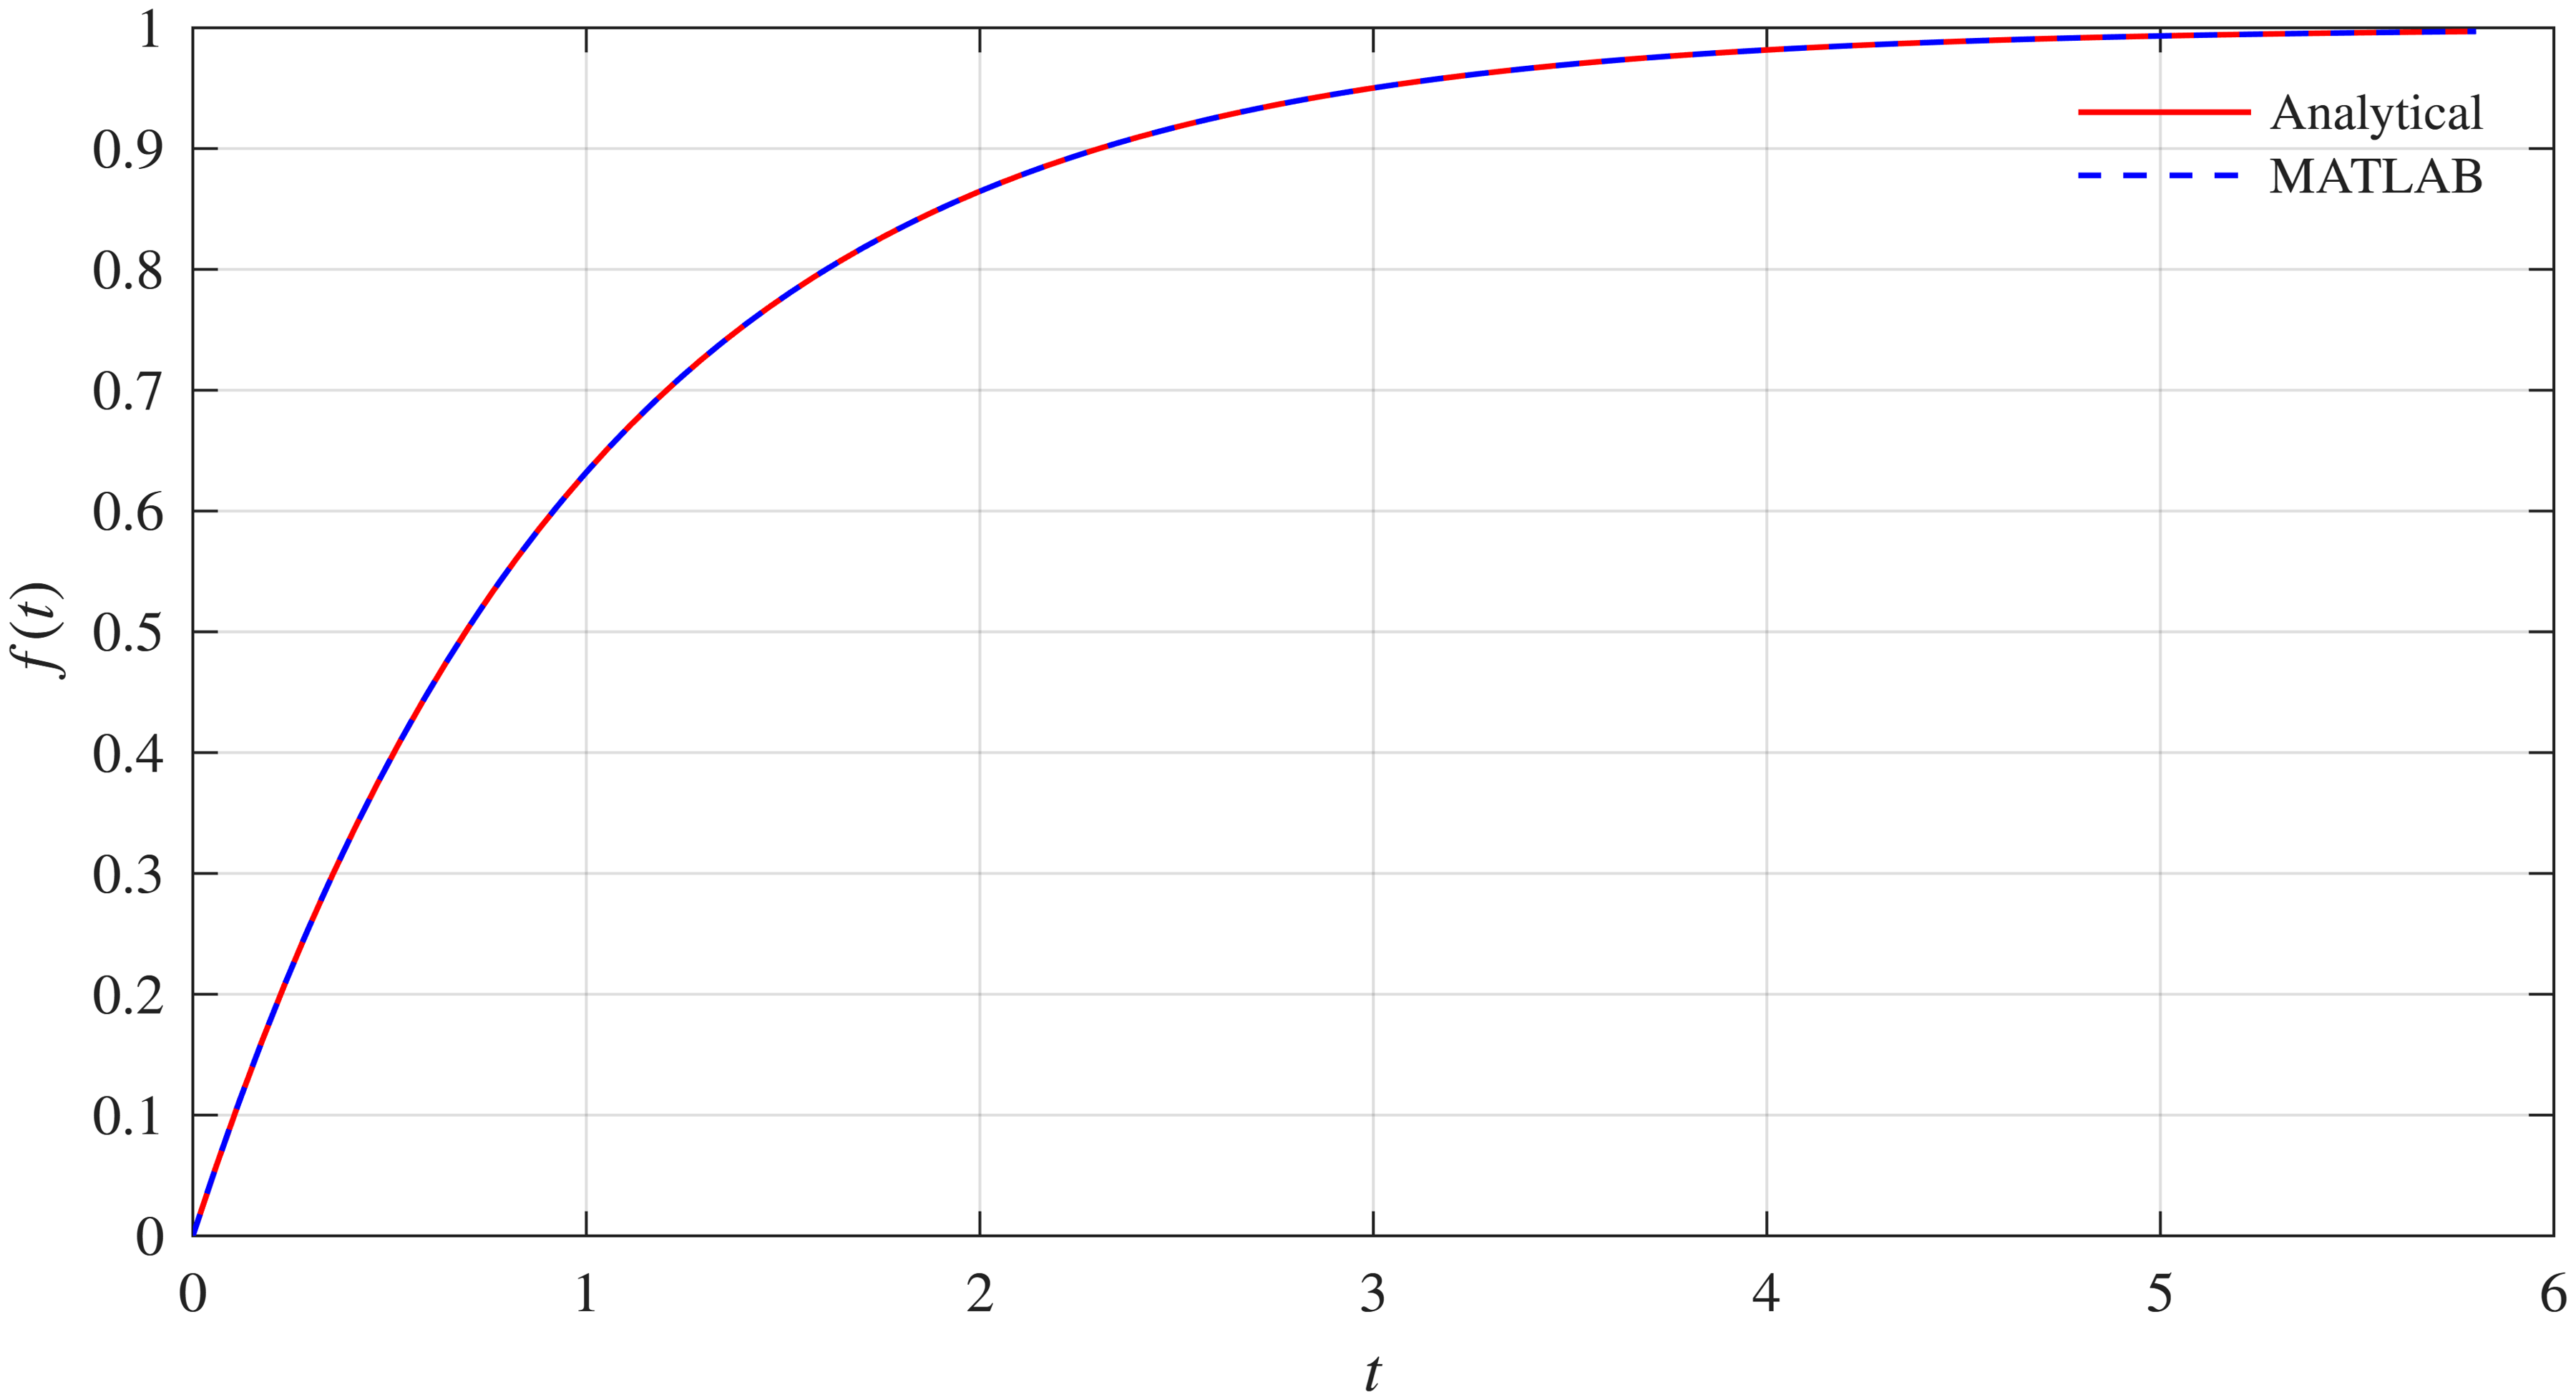
\includegraphics[width=0.75\linewidth]{StepResponse.png}
    \caption{Step Response of $\frac{1}{s+1}$}
    \label{fig:step response first order}
\end{figure}
Notice in our previous example that after $1$ second, $f(t)$ reaches $\sim63\%$ of the final value. This result is obvious when we consider that $1-e^{-t}\approx0.63$ when $t=1$. How long the function takes to reach this threshold is governed by the variable $\tau$. The numerical value of $\tau$ gives the amount of time before the system reaches this $\sim63\%$ threshold. Thus, the time constant determines how quickly a first order system can respond to an input. Of course, gain $K$ dictates the final height in the step response. In the above example, since $K=1$ and the system was subjected to a step response, the final height is $1$.

With just two parameters, we can classify any first order transfer function. We often use such transfer functions to approximate simple processes with a transient start up. Another use case of these first order systems is a \textit{low-pass filter}. We will see this behavior when we study frequency domain behaviors in \autoref{chap:frequency}.

\subsection{Second Order System}
As we have seen when doing Newtonian or Lagrangian mechanics, almost all of our physical systems are dictated by second order equations. Therefore, we can model a huge variety of physical processes by carefully studying these systems. The second order system creates oscillations, which makes it much more complicated than the first order system. The canonical form of the second order system is based on the mass spring damper system. The form of the equation is:\endnote{If you want to derive this form, you may do so in an analogous way to what we did for the first order system.}

\begin{equation}\label{2nd order tf}
G(s)=\frac{\omega_n}{s^2+\zeta\omega_ns+{\omega_n}^2}
\end{equation}

We give each of the variables in this equation a special name because they come up very frequently in engineering and physics applications. We call $\omega_n$ the natural frequency. Under the influence of no damping to the system, this is the angular frequency of the system. In a system like a mass spring damper, it is physically given as the square root of the ratio between the spring constant and the mass:
$$\omega_n=\sqrt{\frac{k}{m}}$$
The term $\zeta$ is called the \textit{damping coefficient}. The value of the damping coefficient must be positive for real systems. At a value of $\zeta=1$, we say that a system is \textit{critically damped}. This is the value at which the system will converge to the input in the least amount of time. For values of $\zeta<1$, the system is called \textit{underdamped}, and will oscillate back and forth before reaching a final value. In control theory, this means the system will have an imaginary component of the eigenvalues. When $\zeta>1$, the system is \textit{overdamped} and will show no oscillation. Here, the eigenvalues of the system will be purely real.

\subsubsection{Second Order Specifications}
The parameters of the second order transfer function are very closely related to the location of the poles of the transfer function. If we understand how to make these adjustments, we can design a second order system that behaves exactly how we want it to. We can summarize all the key features in the complex plane as shown in \autoref{fig:second order poles plot}.

\begin{figure}[ht]
    \centering




\tikzset{every picture/.style={line width=0.75pt}} %set default line width to 0.75pt        

\begin{tikzpicture}[x=0.75pt,y=0.75pt,yscale=-1,xscale=1]
%uncomment if require: \path (0,300); %set diagram left start at 0, and has height of 300

%Straight Lines [id:da3243107301786887] 
\draw    (320.44,50.92) -- (320.44,249.79) ;
%Straight Lines [id:da05704068779201743] 
\draw    (419.87,150.35) -- (221,150.35) ;
%Shape: Arc [id:dp8738705238498384] 
\draw  [draw opacity=0][dash pattern={on 4.5pt off 4.5pt}] (320.44,217.18) .. controls (320.44,217.18) and (320.44,217.18) .. (320.44,217.18) .. controls (283.53,217.18) and (253.61,187.26) .. (253.61,150.35) .. controls (253.61,113.44) and (283.53,83.53) .. (320.44,83.53) -- (320.44,150.35) -- cycle ; \draw  [color={rgb, 255:red, 74; green, 144; blue, 226 }  ,draw opacity=1 ][dash pattern={on 4.5pt off 4.5pt}] (320.44,217.18) .. controls (320.44,217.18) and (320.44,217.18) .. (320.44,217.18) .. controls (283.53,217.18) and (253.61,187.26) .. (253.61,150.35) .. controls (253.61,113.44) and (283.53,83.53) .. (320.44,83.53) ;  
%Straight Lines [id:da6227885653022915] 
\draw [color={rgb, 255:red, 74; green, 144; blue, 226 }  ,draw opacity=1 ] [dash pattern={on 4.5pt off 4.5pt}]  (221,150.35) -- (320.44,150.35) ;
%Straight Lines [id:da7350291413092821] 
\draw [color={rgb, 255:red, 155; green, 155; blue, 155 }  ,draw opacity=1 ]   (320.44,150.35) -- (279,98) ;
%Shape: Arc [id:dp16286487075266098] 
\draw  [draw opacity=0] (290.44,150.35) .. controls (290.44,140.94) and (294.77,132.54) .. (301.55,127.04) -- (320.44,150.35) -- cycle ; \draw [color={rgb, 255:red, 155; green, 155; blue, 155 }  ,draw opacity=1 ]   (290.44,150.35) .. controls (290.44,141.97) and (293.87,134.4) .. (299.41,128.95) ; \draw [shift={(301.55,127.04)}, rotate = 130.03] [fill={rgb, 255:red, 155; green, 155; blue, 155 }  ,fill opacity=1 ][line width=0.08]  [draw opacity=0] (8.93,-4.29) -- (0,0) -- (8.93,4.29) -- cycle    ; 
%Straight Lines [id:da7597435504681186] 
\draw [color={rgb, 255:red, 218; green, 44; blue, 0 }  ,draw opacity=1 ]   (279,98) ;
\draw [shift={(279,98)}, rotate = 45] [color={rgb, 255:red, 218; green, 44; blue, 0 }  ,draw opacity=1 ][line width=0.75]    (-6.15,0) -- (6.15,0)(0,6.15) -- (0,-6.15)   ;
\draw [shift={(279,98)}, rotate = 45] [color={rgb, 255:red, 218; green, 44; blue, 0 }  ,draw opacity=1 ][line width=0.75]    (-6.15,0) -- (6.15,0)(0,6.15) -- (0,-6.15)   ;
%Straight Lines [id:da7948143459768348] 
\draw [color={rgb, 255:red, 155; green, 155; blue, 155 }  ,draw opacity=1 ]   (280,170) -- (317,170) ;
\draw [shift={(320,170)}, rotate = 180] [fill={rgb, 255:red, 155; green, 155; blue, 155 }  ,fill opacity=1 ][line width=0.08]  [draw opacity=0] (7.14,-3.43) -- (0,0) -- (7.14,3.43) -- cycle    ;
\draw [shift={(280,170)}, rotate = 180] [color={rgb, 255:red, 155; green, 155; blue, 155 }  ,draw opacity=1 ][line width=0.75]    (0,4.47) -- (0,-4.47)   ;

% Text Node
\draw (381,72.4) node [anchor=north west][inner sep=0.75pt]    {$\mathbb{C}$};
% Text Node
\draw (313.44,28.4) node [anchor=north west][inner sep=0.75pt]    {$\omega $};
% Text Node
\draw (426.3,140.26) node [anchor=north west][inner sep=0.75pt]    {$\sigma $};
% Text Node
\draw (278,123.4) node [anchor=north west][inner sep=0.75pt]  [color={rgb, 255:red, 155; green, 155; blue, 155 }  ,opacity=1 ]  {$\beta $};
% Text Node
\draw (278,62.4) node [anchor=north west][inner sep=0.75pt]  [color={rgb, 255:red, 74; green, 144; blue, 226 }  ,opacity=1 ]  {$\omega _{n}$};
% Text Node
\draw (351,192.4) node [anchor=north west][inner sep=0.75pt]    {$\zeta =\cos \beta $};
% Text Node
\draw (293,170.4) node [anchor=north west][inner sep=0.75pt]  [color={rgb, 255:red, 155; green, 155; blue, 155 }  ,opacity=1 ]  {$\sigma $};
% Text Node
\draw (351,214.4) node [anchor=north west][inner sep=0.75pt]    {$\sigma =\zeta \omega _{n}$};


\end{tikzpicture}

    \caption{Relation of second order system values to pole locations}
    \label{fig:second order poles plot}
\end{figure}

In the diagram, the poles may exist on any portion of the dotted blue line. The radius of the circular region of the dotted blue line is given by $\omega_n$. The distance from the imaginary axis is $\sigma=\zeta\omega_n$. The angle of the pole from the horizontal is given by the relation $\zeta=\cos\beta$. You may notice that when $\zeta=1$, the angle must be zero. The result is that the critically damped system has both poles lying exactly on the furthest possible point from the origin. Therefore, this is the system which decays the fastest. For greater values, the constraint breaks down because $\cos$ can never achieve a value greater than 1. After this point, the poles stay fixed on the real line. We can represent all possible scenarios as shown in \autoref{fig:pole zeta}:
\begin{figure}[ht]
    \centering

\tikzset{every picture/.style={line width=0.75pt}} %set default line width to 0.75pt        

\begin{tikzpicture}[x=0.75pt,y=0.75pt,yscale=-0.8,xscale=0.8]
%uncomment if require: \path (0,300); %set diagram left start at 0, and has height of 300

%Straight Lines [id:da5282441780493525] 
\draw    (100,70) -- (100,210) ;
%Straight Lines [id:da7423345996136652] 
\draw    (140,140) -- (30,140) ;
%Shape: Arc [id:dp3799084322094477] 
\draw  [draw opacity=0][dash pattern={on 4.5pt off 4.5pt}] (100,192.28) .. controls (100,192.28) and (100,192.28) .. (100,192.28) .. controls (71.13,192.28) and (47.72,168.87) .. (47.72,140) .. controls (47.72,111.13) and (71.13,87.72) .. (100,87.72) -- (100,140) -- cycle ; \draw  [color={rgb, 255:red, 74; green, 144; blue, 226 }  ,draw opacity=1 ][dash pattern={on 4.5pt off 4.5pt}] (100,192.28) .. controls (100,192.28) and (100,192.28) .. (100,192.28) .. controls (71.13,192.28) and (47.72,168.87) .. (47.72,140) .. controls (47.72,111.13) and (71.13,87.72) .. (100,87.72) ;  
%Straight Lines [id:da7728653865582944] 
\draw    (30,60) -- (527,60) ;
\draw [shift={(530,60)}, rotate = 180] [fill={rgb, 255:red, 0; green, 0; blue, 0 }  ][line width=0.08]  [draw opacity=0] (8.93,-4.29) -- (0,0) -- (8.93,4.29) -- cycle    ;
%Straight Lines [id:da3227845193340638] 
\draw [color={rgb, 255:red, 218; green, 44; blue, 0 }  ,draw opacity=1 ]   (100,87.72) ;
\draw [shift={(100,87.72)}, rotate = 45] [color={rgb, 255:red, 218; green, 44; blue, 0 }  ,draw opacity=1 ][line width=0.75]    (-6.15,0) -- (6.15,0)(0,6.15) -- (0,-6.15)   ;
\draw [shift={(100,87.72)}, rotate = 45] [color={rgb, 255:red, 218; green, 44; blue, 0 }  ,draw opacity=1 ][line width=0.75]    (-6.15,0) -- (6.15,0)(0,6.15) -- (0,-6.15)   ;
%Straight Lines [id:da8934356003374623] 
\draw [color={rgb, 255:red, 218; green, 44; blue, 0 }  ,draw opacity=1 ]   (100,192.28) ;
\draw [shift={(100,192.28)}, rotate = 45] [color={rgb, 255:red, 218; green, 44; blue, 0 }  ,draw opacity=1 ][line width=0.75]    (-6.15,0) -- (6.15,0)(0,6.15) -- (0,-6.15)   ;
\draw [shift={(100,192.28)}, rotate = 45] [color={rgb, 255:red, 218; green, 44; blue, 0 }  ,draw opacity=1 ][line width=0.75]    (-6.15,0) -- (6.15,0)(0,6.15) -- (0,-6.15)   ;
%Straight Lines [id:da474881892975197] 
\draw    (230,70) -- (230,210) ;
%Straight Lines [id:da841826413240565] 
\draw    (270,140) -- (160,140) ;
%Shape: Arc [id:dp4202329030763605] 
\draw  [draw opacity=0][dash pattern={on 4.5pt off 4.5pt}] (230,192.28) .. controls (201.13,192.28) and (177.72,168.87) .. (177.72,140) .. controls (177.72,111.13) and (201.13,87.72) .. (230,87.72) -- (230,140) -- cycle ; \draw  [color={rgb, 255:red, 74; green, 144; blue, 226 }  ,draw opacity=1 ][dash pattern={on 4.5pt off 4.5pt}] (230,192.28) .. controls (201.13,192.28) and (177.72,168.87) .. (177.72,140) .. controls (177.72,111.13) and (201.13,87.72) .. (230,87.72) ;  
%Straight Lines [id:da86644447643968] 
\draw [color={rgb, 255:red, 218; green, 44; blue, 0 }  ,draw opacity=1 ]   (202.28,96) ;
\draw [shift={(202.28,96)}, rotate = 45] [color={rgb, 255:red, 218; green, 44; blue, 0 }  ,draw opacity=1 ][line width=0.75]    (-6.15,0) -- (6.15,0)(0,6.15) -- (0,-6.15)   ;
\draw [shift={(202.28,96)}, rotate = 45] [color={rgb, 255:red, 218; green, 44; blue, 0 }  ,draw opacity=1 ][line width=0.75]    (-6.15,0) -- (6.15,0)(0,6.15) -- (0,-6.15)   ;
%Straight Lines [id:da3524379099285829] 
\draw [color={rgb, 255:red, 218; green, 44; blue, 0 }  ,draw opacity=1 ]   (202.28,184) ;
\draw [shift={(202.28,184)}, rotate = 45] [color={rgb, 255:red, 218; green, 44; blue, 0 }  ,draw opacity=1 ][line width=0.75]    (-6.15,0) -- (6.15,0)(0,6.15) -- (0,-6.15)   ;
\draw [shift={(202.28,184)}, rotate = 45] [color={rgb, 255:red, 218; green, 44; blue, 0 }  ,draw opacity=1 ][line width=0.75]    (-6.15,0) -- (6.15,0)(0,6.15) -- (0,-6.15)   ;
%Straight Lines [id:da05358277976389181] 
\draw    (360,70) -- (360,210) ;
%Straight Lines [id:da9078928799626685] 
\draw    (400,140) -- (290,140) ;
%Shape: Arc [id:dp7916297070988959] 
\draw  [draw opacity=0][dash pattern={on 4.5pt off 4.5pt}] (360,192.28) .. controls (331.13,192.28) and (307.72,168.87) .. (307.72,140) .. controls (307.72,111.13) and (331.13,87.72) .. (360,87.72) -- (360,140) -- cycle ; \draw  [color={rgb, 255:red, 74; green, 144; blue, 226 }  ,draw opacity=1 ][dash pattern={on 4.5pt off 4.5pt}] (360,192.28) .. controls (331.13,192.28) and (307.72,168.87) .. (307.72,140) .. controls (307.72,111.13) and (331.13,87.72) .. (360,87.72) ;  
%Straight Lines [id:da7803510026730456] 
\draw [color={rgb, 255:red, 218; green, 44; blue, 0 }  ,draw opacity=1 ]   (308,140) ;
\draw [shift={(308,140)}, rotate = 45] [color={rgb, 255:red, 218; green, 44; blue, 0 }  ,draw opacity=1 ][line width=0.75]    (-6.15,0) -- (6.15,0)(0,6.15) -- (0,-6.15)   ;
\draw [shift={(308,140)}, rotate = 45] [color={rgb, 255:red, 218; green, 44; blue, 0 }  ,draw opacity=1 ][line width=0.75]    (-6.15,0) -- (6.15,0)(0,6.15) -- (0,-6.15)   ;
%Straight Lines [id:da12461779159195308] 
\draw    (490,70) -- (490,210) ;
%Straight Lines [id:da753991406913465] 
\draw    (530,140) -- (420,140) ;
%Shape: Arc [id:dp33171387660033513] 
\draw  [draw opacity=0][dash pattern={on 4.5pt off 4.5pt}] (490,192.28) .. controls (461.13,192.28) and (437.72,168.87) .. (437.72,140) .. controls (437.72,111.13) and (461.13,87.72) .. (490,87.72) -- (490,140) -- cycle ; \draw  [color={rgb, 255:red, 74; green, 144; blue, 226 }  ,draw opacity=1 ][dash pattern={on 4.5pt off 4.5pt}] (490,192.28) .. controls (461.13,192.28) and (437.72,168.87) .. (437.72,140) .. controls (437.72,111.13) and (461.13,87.72) .. (490,87.72) ;  
%Straight Lines [id:da7947899663397748] 
\draw [color={rgb, 255:red, 218; green, 44; blue, 0 }  ,draw opacity=1 ]   (456,140) ;
\draw [shift={(456,140)}, rotate = 45] [color={rgb, 255:red, 218; green, 44; blue, 0 }  ,draw opacity=1 ][line width=0.75]    (-6.15,0) -- (6.15,0)(0,6.15) -- (0,-6.15)   ;
\draw [shift={(456,140)}, rotate = 45] [color={rgb, 255:red, 218; green, 44; blue, 0 }  ,draw opacity=1 ][line width=0.75]    (-6.15,0) -- (6.15,0)(0,6.15) -- (0,-6.15)   ;
%Straight Lines [id:da7212782141665846] 
\draw [color={rgb, 255:red, 218; green, 44; blue, 0 }  ,draw opacity=1 ]   (426,140) ;
\draw [shift={(426,140)}, rotate = 45] [color={rgb, 255:red, 218; green, 44; blue, 0 }  ,draw opacity=1 ][line width=0.75]    (-6.15,0) -- (6.15,0)(0,6.15) -- (0,-6.15)   ;
\draw [shift={(426,140)}, rotate = 45] [color={rgb, 255:red, 218; green, 44; blue, 0 }  ,draw opacity=1 ][line width=0.75]    (-6.15,0) -- (6.15,0)(0,6.15) -- (0,-6.15)   ;

% Text Node
\draw (280,52.6) node [anchor=south] [inner sep=0.75pt]    {$\text{Increasing} \ \zeta $};
% Text Node
\draw (100,213.4) node [anchor=north] [inner sep=0.75pt]    {$\zeta =0$};
% Text Node
\draw (230,213.4) node [anchor=north] [inner sep=0.75pt]    {$0< \zeta < 1$};
% Text Node
\draw (360,213.4) node [anchor=north] [inner sep=0.75pt]    {$\zeta =1$};
% Text Node
\draw (490,213.4) node [anchor=north] [inner sep=0.75pt]    {$\zeta  >1$};


\end{tikzpicture}
    \caption{Evolution of pole positions in terms of $\zeta$}
    \label{fig:pole zeta}
\end{figure}


Using these system parameters, it is possible to come up with time domain specifications for our control system. Most of the criteria for such systems are usually given in terms of the step response of a second order system. Some of the typical criteria are shown in \autoref{fig:2nd order step}.

\begin{figure}[ht]
    \centering
    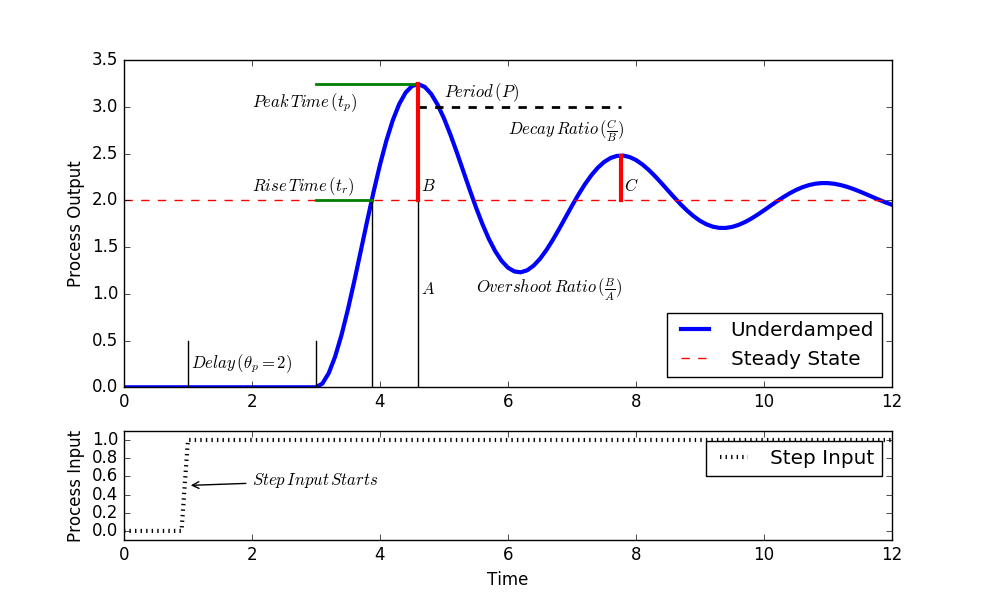
\includegraphics[width=\linewidth]{Images/second_order_graphical_fit.png}
    \caption{Step response of a second order transfer function}
    \label{fig:2nd order step}
\end{figure}
\todo{Redo this figure myself}

A list of the time domain specifications in terms of the canonical variables is shown below:
\begin{align}
     M_p&=  \exp(-\pi\zeta/\sqrt{1-\zeta^2})\\
     t_s(2\%)&= \frac{4}{\sigma}\\
     t_p&=\frac{\pi}{\omega_n\sqrt{1-\zeta^2}}\\
     t_r&=\frac{\pi-\cos^{-1}(\zeta)}{\omega_n\sqrt{1-\zeta^2}}
\end{align}

\subsection{Higher Order Systems}
Very often, our system will have 3 or more poles. In this case, the first or second order descriptions will not be exactly correct. However, it is the case that we can always combine the response of the first and second order systems in order to achieve the same result as a higher order system. Consider a third order system:
$$G_3(s)=\frac{1}{s^3+2s^2+2s+1}$$
We can decompose this system into a first order system and a second order system:
$$G_3(s)=G_1(s)G_2(s)=\frac{K}{s\tau+1}\frac{\omega_n}{s^2+\zeta\omega_ns+\omega_n^2}$$
The appropriate generalization may be done for higher order systems. From here, the exercise becomes an algebraic one. We simply match the terms of the third order polynomial to find the appropriate values. We can start from these conditions (on the numerator and 0th order denominator terms):
\begin{gather}
K\omega_n=1,\quad \omega_n^2=1
\end{gather}
Which make it obvious that both $\omega_n$ and $K$ are necessarily 1. From here, we can expand the rest of the expression:
$$G_3(s)=\frac{1}{s^3+2s^2+s+1}=\frac{1}{\tau s^3+\zeta\tau s^2+s\tau +s^2+\zeta s+1}$$
And we find the following relations:
\begin{gather}
    \tau s^3=s^3\rightarrow\tau=1\\
    2s^2=s^2(\zeta\tau+1)\rightarrow\zeta=1
\end{gather}
This exact approach will not now always work. In general, we require that we have as many degrees of freedom as the number of poles in the system. In general, we would generate a polynomial of the form:
$$\frac{1}{(s+a)(s^2+bs+c)}$$
This factorization may be easily computed with a tool like MATLAB or Python. In MATLAB, we can utilize the following command:
\begin{matlabscript}
syms s
y = s^3+2*s^2+s+1;
factor(y, s, 'FactorMode', 'real')
\end{matlabscript}
Notice that this function does not have a simple factorization like our previous result. MATLAB will return the following:
$$\begin{pmatrix}
s+1.75487 & s^2 +0.24512\,s+0.56984
\end{pmatrix}$$
Now we have values for $a,b$ and $c$ and can construct the appropriate first and second order functions.
\begin{exercise}[Response of Third Order System]
Consider the example above where the third order transfer function takes the form:
$$G(s)=\frac{1}{s^3+2s^2+s+1}$$
We have already shown the factorization can be achieved with MATLAB.
\begin{enumerate}
    \item Find the poles for the second order transfer function of this system
    \item Plot the step response of the first order system, second order system, and third order system on the same plot
\end{enumerate}
\end{exercise}

If you complete the above exercise, you will find that the second order response dominates the response of this system. Why? This occurs because the second order system has its poles closer to the origin. This means that these poles will decay more slowly than the poles further from the origin. As a result, the second order transfer function with the poles closer to the origin will dominate the response of the system. Since the poles are closer to the origin, we call them \textit{dominant} poles of the system.

Often, the true response of our system will have many different modes and be complex. Often we can simplify our system analysis (at least in the beginning) to just include these dominant poles, which will give us a first or second order transfer function which describes the dynamics of the system. This type of reduction is often very useful in flight dynamics systems. If we imagine controlling an aircraft or rocket, there are many modes for a control surface. There may be vibrations in the control surface, various harmonics in the structure, or other high order effects. Typically we can ignore these in control design and consider only the most important delay term(s).

\section{System Type}
Before we actually start designing controllers for systems, we have a few last nuances of transfer functions to cover. The \textit{system type} tells us the polynomial degree of an input where our system has a nonzero constant error. To get started, we need to find the error in our transfer function. If we do the same algebraic analysis as before, we will find that the transfer function from the input to the error is given by:
$$\frac{E(s)}{R(s)}=\frac{1}{1+GH}$$
With a transfer function description of the error, we can use the final value theorem in order to find if the error in the system eventually decreases to zero under a certain input.

To motivate this a bit further, let's consider a simple system with no controller and no feedback. We're going to choose the transfer function of the system to be something simple: $\frac{1}{s+1}$.

\begin{figure}[ht]
    \centering


\tikzset{every picture/.style={line width=0.75pt}} %set default line width to 0.75pt        

\begin{tikzpicture}[x=0.75pt,y=0.75pt,yscale=-1,xscale=1]
%uncomment if require: \path (0,300); %set diagram left start at 0, and has height of 300

%Flowchart: Process [id:dp22985398749031094] 
\draw  [fill={rgb, 255:red, 74; green, 144; blue, 226 }  ,fill opacity=0.43 ] (280,125) -- (360,125) -- (360,175) -- (280,175) -- cycle ;
%Straight Lines [id:da22245740194670927] 
\draw    (360,150) -- (417,150) ;
\draw [shift={(420,150)}, rotate = 180] [fill={rgb, 255:red, 0; green, 0; blue, 0 }  ][line width=0.08]  [draw opacity=0] (8.93,-4.29) -- (0,0) -- (8.93,4.29) -- cycle    ;
%Straight Lines [id:da8656358522969507] 
\draw    (220,150) -- (277,150) ;
\draw [shift={(280,150)}, rotate = 180] [fill={rgb, 255:red, 0; green, 0; blue, 0 }  ][line width=0.08]  [draw opacity=0] (8.93,-4.29) -- (0,0) -- (8.93,4.29) -- cycle    ;

% Text Node
\draw (250,146.6) node [anchor=south] [inner sep=0.75pt]    {$R( s)$};
% Text Node
\draw (390,146.6) node [anchor=south] [inner sep=0.75pt]    {$Y( s)$};
% Text Node
\draw (320,149) node    {$\frac{1}{s+1}$};


\end{tikzpicture}    
    \caption{Open Loop System Response}
    \label{fig:open loop sys blk diagram}
\end{figure}

When we are concerned with \textit{system type}, we want to know how this system responds to an input of increasing order. When the system is unable to track the input, we know the system type. We'll define a progression of inputs, each of which are the integral of the previous one. We start with the impulse function, $\delta(t)$. As long as our system is stable, it will achieve zero error in response to an impulse response. Integrating the impulse gives the step response, $\frac{1}{s}$ in the Laplace domain. Integrating again gives the ramp response, which is a linearly increasing input. We can keep integrating the input to subject the system to more and more aggressive inputs. The system type is the largest order of input for which a system can achieve zero steady state error. If our system can achieve no steady state error when subjected to a delta function, it is a system type of 0. In response to a step response, it is a system type of 1, and so on.

\begin{example}[Determining system type]
Lets subject the transfer function $\frac{1}{s+2}$ to a step input, which is of the form $\frac{1}{s}$. In the Laplace domain, we have a multiplication:
$$\frac{1}{s(s+2)}$$
We can now apply final value theorem, which will tell us the condition at $t\rightarrow\infty$ since this transfer function is stable:
$$\lim_{s\rightarrow0}\frac{s}{s(s+2)}=\lim_{s\rightarrow0}\frac{1}{s+2}=\frac{1}{2}$$So, we see that when subjected to a unit step, our function eventually reaches the condition that $y(t)=\frac{1}{2}$, not the original input of $1$. So, this function has a steady state error! It will never reach the input condition, no matter how long we wait. Let's now try a ramp input now, which we classify as $\frac{1}{s^2}$. This gives our total function:
$$\frac{1}{s^2(s+1)}$$
and the application of the final value theorem:
$$\lim_{s\rightarrow0}\frac{s}{s^2(s+1)}=\lim_{s\rightarrow0}\frac{1}{s(s+1)}=\infty$$
As we can see, in such a system our final value theorem tells us that such a system will build up infinite error with respect to the ramp input. Finally, let's try the simplest input, the delta function. Since the delta function is simply 1 in the Laplace domain, we apply final value theorem on the original function multiplied by $s$:
$$\lim_{s\rightarrow0}\frac{s}{(s+2)}=0$$
Since the system can only achieve zero steady state error when subjected to the delta function, we say that the system is a type-0 system.
\end{example}

One method of determining system type is to look at the number of `integrators' in the system. That is, we look at how many $\frac{1}{s}$ terms are present in the equation. We can easily tell that the transfer function:
$$G(s)=\frac{3}{s(s+2)}$$
must be a type 1 system because there is one free $\frac{1}{s}$ term. Likewise, the system
$$G(s)=\frac{s^2}{s^4(s+1)}$$
is a type 2 system, because we have $s^2$ in the denominator after the simplification of the rational expression.

The concept of system type tells us one thing that is particularly important. An integrator can reduce or remove steady state error from a system. With that knowledge, we can see why controllers like the PID controller have an `integrator' component. This exists to reduce the steady state error in a system!


\section{Realizing Transfer Functions}

As a last note for this chapter, we should note some of the limitations in writing transfer functions for control systems. 

\subsection{Proper Transfer Functions}
Earlier, we stated that we our concern was mostly with transfer functions that look like:
$$G(s)=\frac{N(s)}{D(s)}=\frac{(s-z_1)(s-z_2)\cdots(s-z_m)}{(s-p_1)(s-p_2)\cdots(s-p_n)}$$
Firstly, we want our transfer functions to be \textit{proper} in almost all cases. This means that the degree of the numerator should be less than or equal to the degree of the denominator ($m\le n$). When this is the case, we call the transfer function proper. The reason for this is somewhat subtle, but it boils down to the fact that no physical system will ever have a numerator with a degree that is greater than the denominator. As an example, let's consider a plant which has an improper transfer function:
$$G(s)=s$$
Of course, this looks like a differentiator in the time domain:
$$g(t)=\frac{du}{dt}$$
For now, we will consider applying no control to the system. We will just subject the system to an impulse function $u=\delta(t)$. The response of the system is the \textit{derivative} of the impulse function!
$$g(t)=\delta'(t)$$
This is obviously nonphysical, it means that output will have an infinite spike. Any improper transfer function will exhibit such behavior. The result is that we do not want such behaviors in physical systems. 

Most of the time, we do not see improper transfer functions arise when we derive systems from correct equations of motion. However, we can see transfer functions that are not \textit{strictly proper}. A strictly proper transfer function is one in which the degree of the numerator is less than the degree of the denominator. However, there is a much easier fix for such systems. We may always write a system where the degree of the numerator and denominator are equal as:
$$G(s)=\frac{(s-z_1)(s-z_2)\cdots(s-z_n)}{(s-p_1)(s-p_2)\cdots(s-p_n)}=\frac{(s-z_1)(s-z_2)\cdots(s-z_{n-1})}{(s-p_1)(s-p_2)\cdots(s-p_n)}+D$$
To actually compute a strictly proper transfer function from a proper one, we use long division.
\begin{example}[Constructing strictly proper transfer functions]

Let's consider the function:
$$G(s)=\frac{s^3+2s^2+1}{s^3+2s}$$ To make such a function strictly proper, we use polynomial long division. We place the numerator inside as the dividend and the denominator as the divisor:
$$\begin{array}{r}
1\phantom{)}   \\
s^3+2s{\overline{\smash{\big)}\,s^2+2s^2+1\phantom{)}}}\\
\underline{-~\phantom{(}(s^3+2s)\phantom{-b)}}\\
2s^2-2s+1\phantom{)}
\end{array}$$
Our final result is the result of the long division with the remainder divided by the original function. Typically, only one step is required to reduce the order sufficiently. In this case, our strictly proper transfer function is:
$$G(s)=\frac{2s^2-2s+1}{s^3+2s}+1$$
\end{example}

\subsection{Rational Transfer Functions}

Our other concern with writing transfer functions is that not all types of functions are represented as polynomial equations. A very common example is a system with delay, where we may have a term like $e^{-st}$ present. Unfortunately, we cannot model such a function using a polynomial equation. Any time we have a function like $\sin(s)$ or $e^{-st}$ present, we cannot use the standard tools of control theory. For delays, this is a big problem! Up until now, we have ignored a pretty crucial part of system dynamics, which is delay. With an ideal transfer function, we don't get any delay in our system dynamics, since our sensors read things off exactly as they happen. This is not a physical reality, though, and we should take a bit of time to consider ways to model systems with delay. While we cannot get exact solutions to such transfer functions, we can approximate them using Pad/'e approximants.

\subsubsection{Pad\'{e} Approximants}

Pad\'e approximants can generally model any function near a specific operating point, but in control theory their primary use is in modeling delays. I will not cover how to calculate the Pad\'e approximant, as the general form can be somewhat intensive. Since a  Pad\'e approximant is a rational polynomial expression, we must define the order of the numerator and denominator. The general form is:
$$\frac{a_0+a_1x+\cdots+a_mx^m}{1+b_1x+b_2x^2+\cdots+b_nx^n}$$
It is required that $m\ge0$ and $n\ge1$. In control theory, we typically also require that the function is proper (though not strictly proper).

In MATLAB, we can use the \texttt{pade} function in two ways. If we are using symbolic variables, it is possible to find the pad\'e approximant of a function \texttt{f} as:
\begin{matlabscript}{Symbolic Pad\'e approximant}
syms x

f = sin(x)

% input function, variable, center point, and order
approxPade = pade(f,x,0,'Order',[3 3])
approxTaylor = taylor(f,x,0,'Order',4)

% plot the result
figure;
fplot(sin(x),[-2,2],'DisplayName', '$\sin(x)$')
hold on
fplot(approxPade,[-2,2], 'DisplayName', 'Pade')
fplot(approxTaylor,[-2,2], 'DisplayName', 'Taylor')
legend(Location="northwest")
title('Comparison of Approximations')
xlabel('$x$')
ylabel('$f(x)$')
    
\end{matlabscript}

We can see that the resulting Pad\'e approximant matches the function much better than the Taylor series as shown in \autoref{fig:taylor v pade}.

\begin{figure}[ht]
    \centering
    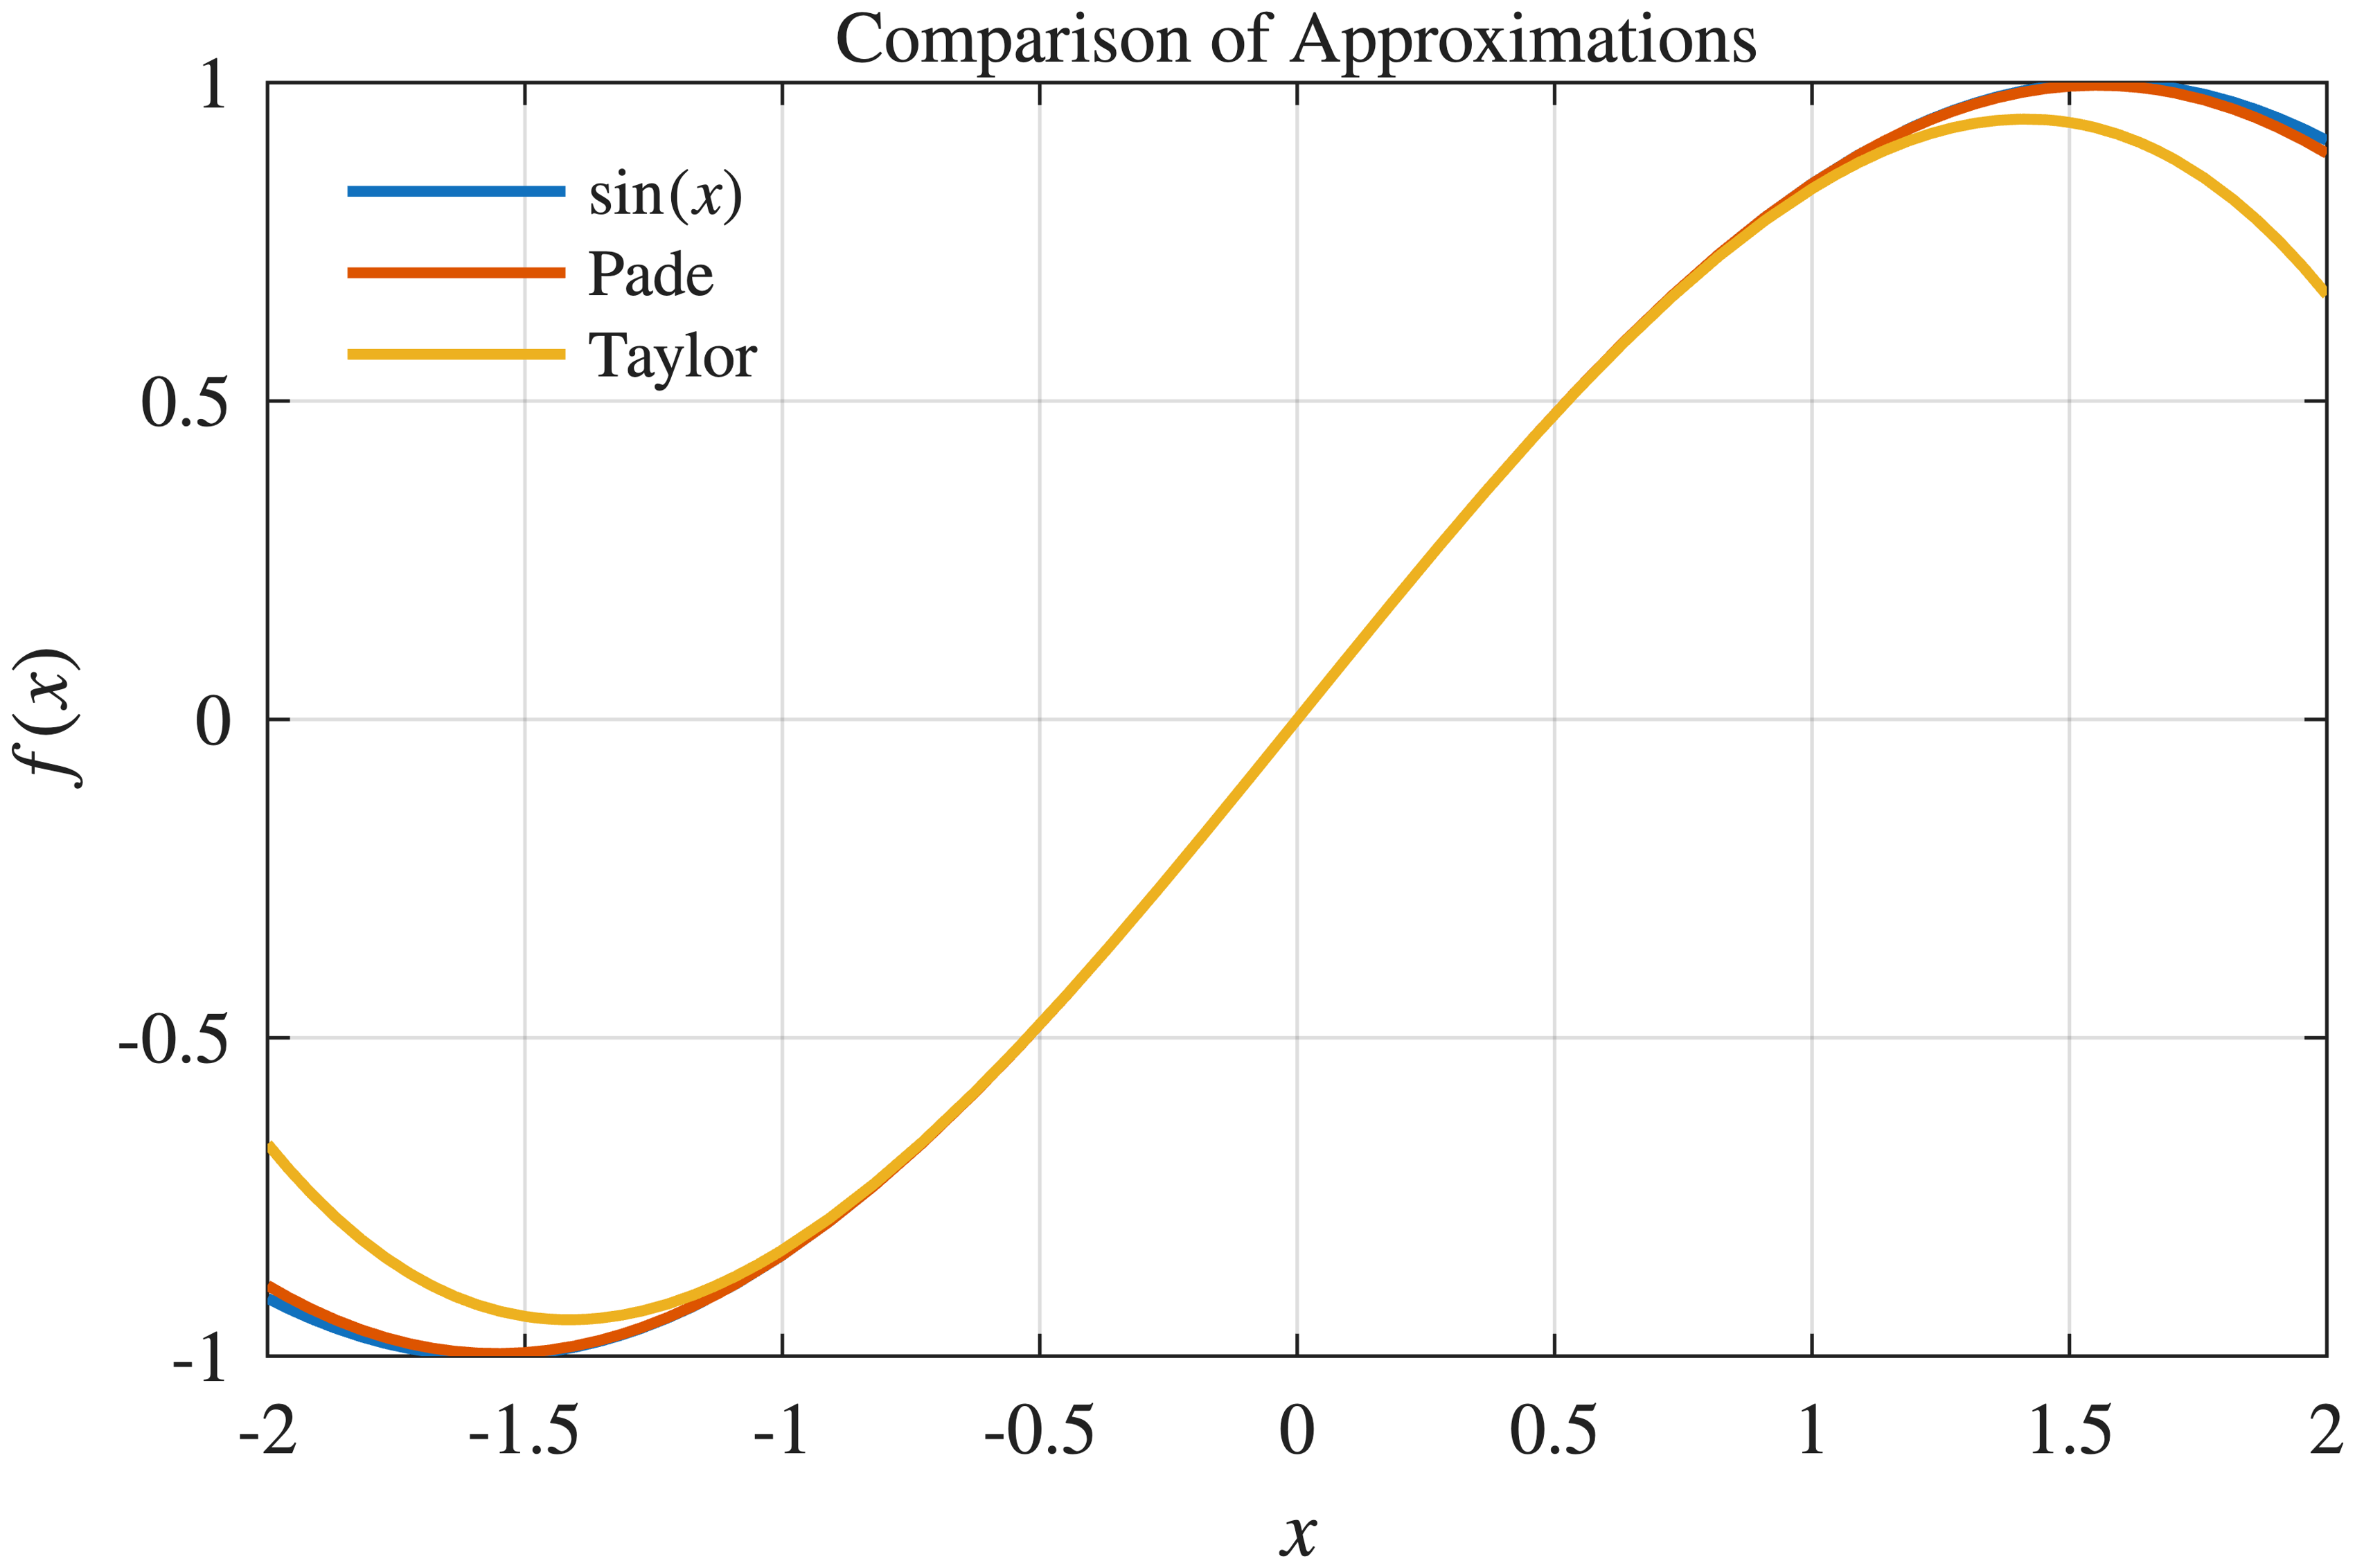
\includegraphics[width=1\linewidth]{ApproximationComp2.png}
    \caption{Comparison of Taylor series and Pad\'e approximations of the sine function}
    \label{fig:taylor v pade}
\end{figure}

This symbolic approach allows us to compute the Pad\'e approximant for an arbitrary functions $f$ (so long as they are analytic around the point of consideration). 

Because we often want to apply the Pad\'e approximant to control systems, MATLAB has a built in function for writing the transfer function of a delay. We use the same function \texttt{pade}, which is interpreted differently when the input is not symbolic. We specify the delay time in seconds and the order of the approximation.
\begin{matlabscript}{Pad\'e approximant for delay}
tau = 0.5;
n = 2;

pade(tau,n)
\end{matlabscript}

This will output a plot showing a true time delay as compared to the Pad/'e approximation, and the phase plot of the true delay as compared to the phase of the approximation (more on this in \autoref{chap:frequency}). The coefficients of the transfer function can be output simply by doing \texttt{[num,den] = pade(tau,n)}.


\section{Practice Problems}

\begin{exercise}[DC Motor]
\begin{enumerate}
    \item Consider a simple control system for a DC motor. The motors angle can be modeled as a simple transfer function between the input voltage $V$ and it's output $\theta$. The controller, $K_p+\frac{K_i}{s}$ is shown to the left of the motor transfer function. This system is shown below in the block diagram in \autoref{fig:motor angle control}:
    \begin{figure}[H]
        \centering
        

\tikzset{every picture/.style={line width=0.75pt}} %set default line width to 0.75pt        

\begin{tikzpicture}[x=0.75pt,y=0.75pt,yscale=-0.9,xscale=0.9]
%uncomment if require: \path (0,300); %set diagram left start at 0, and has height of 300

%Flowchart: Process [id:dp47885050914751914] 
\draw  [fill={rgb, 255:red, 74; green, 144; blue, 226 }  ,fill opacity=0.43 ] (240,145) -- (320,145) -- (320,195) -- (240,195) -- cycle ;
%Flowchart: Process [id:dp27586918225087564] 
\draw  [fill={rgb, 255:red, 74; green, 144; blue, 226 }  ,fill opacity=0.43 ] (380,145) -- (460,145) -- (460,195) -- (380,195) -- cycle ;
%Straight Lines [id:da004910272094030388] 
\draw    (320,170) -- (377,170) ;
\draw [shift={(380,170)}, rotate = 180] [fill={rgb, 255:red, 0; green, 0; blue, 0 }  ][line width=0.08]  [draw opacity=0] (8.93,-4.29) -- (0,0) -- (8.93,4.29) -- cycle    ;
%Straight Lines [id:da2888199737278474] 
\draw    (460,170) -- (517,170) ;
\draw [shift={(520,170)}, rotate = 180] [fill={rgb, 255:red, 0; green, 0; blue, 0 }  ][line width=0.08]  [draw opacity=0] (8.93,-4.29) -- (0,0) -- (8.93,4.29) -- cycle    ;
%Straight Lines [id:da3783579579400398] 
\draw    (120,170) -- (167,170) ;
\draw [shift={(170,170)}, rotate = 180] [fill={rgb, 255:red, 0; green, 0; blue, 0 }  ][line width=0.08]  [draw opacity=0] (8.93,-4.29) -- (0,0) -- (8.93,4.29) -- cycle    ;
%Straight Lines [id:da8246631595636741] 
\draw    (470,170) -- (470,230) ;
%Shape: Circle [id:dp187718705079432] 
\draw   (170,170) .. controls (170,161.72) and (176.72,155) .. (185,155) .. controls (193.28,155) and (200,161.72) .. (200,170) .. controls (200,178.28) and (193.28,185) .. (185,185) .. controls (176.72,185) and (170,178.28) .. (170,170) -- cycle ;
%Straight Lines [id:da23452296039315146] 
\draw    (185,230) -- (185,188) ;
\draw [shift={(185,185)}, rotate = 90] [fill={rgb, 255:red, 0; green, 0; blue, 0 }  ][line width=0.08]  [draw opacity=0] (8.93,-4.29) -- (0,0) -- (8.93,4.29) -- cycle    ;
%Straight Lines [id:da9138966679831894] 
\draw    (185,230) -- (470,230) ;
%Straight Lines [id:da8765530681435604] 
\draw    (200,170) -- (237,170) ;
\draw [shift={(240,170)}, rotate = 180] [fill={rgb, 255:red, 0; green, 0; blue, 0 }  ][line width=0.08]  [draw opacity=0] (8.93,-4.29) -- (0,0) -- (8.93,4.29) -- cycle    ;

% Text Node
\draw (145,166.6) node [anchor=south] [inner sep=0.75pt]    {$\theta _{r}$};
% Text Node
\draw (350,164.6) node [anchor=south] [inner sep=0.75pt]    {$V$};
% Text Node
\draw (490,164.6) node [anchor=south] [inner sep=0.75pt]    {$\theta $};
% Text Node
\draw (171,168) node [anchor=west] [inner sep=0.75pt]  [font=\scriptsize]  {$+$};
% Text Node
\draw (180,177.5) node [anchor=west] [inner sep=0.75pt]  [font=\scriptsize]  {$-$};
% Text Node
\draw (220,166.6) node [anchor=south] [inner sep=0.75pt]    {$E$};
% Text Node
\draw (280,170) node    {$K_{p} +\frac{K_{i}}{s}$};
% Text Node
\draw (420,170) node    {$\frac{1}{s+1}$};


\end{tikzpicture}

        \caption{Motor Angle Control}
        \label{fig:motor angle control}
    \end{figure}
    \begin{enumerate}
        \item Find the open-loop transfer function of the system. This is the transfer function that you would find if the sum block did not have anything being subtracted. Call this transfer function $L(s)$.
        \item Find the closed loop transfer function of the system, given as $\frac{\theta}{\theta_r}$.
        \item Take $K_p=K_i=1$ and $\theta_r=\frac{1}{s}$. What is the final value of $\theta$ as $t\rightarrow\infty$?
        \item Compute $1+L(s)$. How does this compare with the closed loop transfer function that you found?
    \end{enumerate}
\end{enumerate}

\end{exercise}

\newpage
\printendnotes

\chapter{Root Locus Design}\label{chap:root locus}

In our exploration of transfer functions, we discovered that we can change the stability of a system by changing the gain $K$.  This turns out to be very powerful for designing controllers, and we will utilize this capability in our first method of controller design: the \textit{root locus} design method.

With root locus design, we are going to use the pole-zero plot to explore how changing a gain $K$ will alter the pole locations of our function. We look at the locus of all points in the pole-zero plot, given by different values of $K$, which allows us to pick a good value of $K$ to control our system. With this method, we can design a number of controllers, including PID controllers and lead-lag compensators.

\section{Feedback Control}
To design a system via the root locus method, we first need to know what our systems look like. We'll restrict our focus to a few prototypical systems, like shown in \autoref{fig:root locus}.
\begin{figure}[ht]
    \centering



\tikzset{every picture/.style={line width=0.75pt}} %set default line width to 0.75pt        

\begin{tikzpicture}[x=0.75pt,y=0.75pt,yscale=-1,xscale=1]
%uncomment if require: \path (0,300); %set diagram left start at 0, and has height of 300

%Flowchart: Process [id:dp1875054016665445] 
\draw  [fill={rgb, 255:red, 74; green, 144; blue, 226 }  ,fill opacity=0.43 ] (370,110) -- (450,110) -- (450,150) -- (370,150) -- cycle ;
%Straight Lines [id:da7499236715272949] 
\draw    (450,130) -- (537,130) ;
\draw [shift={(540,130)}, rotate = 180] [fill={rgb, 255:red, 0; green, 0; blue, 0 }  ][line width=0.08]  [draw opacity=0] (8.93,-4.29) -- (0,0) -- (8.93,4.29) -- cycle    ;
%Straight Lines [id:da8364498609050864] 
\draw    (150,130) -- (197,130) ;
\draw [shift={(200,130)}, rotate = 180] [fill={rgb, 255:red, 0; green, 0; blue, 0 }  ][line width=0.08]  [draw opacity=0] (8.93,-4.29) -- (0,0) -- (8.93,4.29) -- cycle    ;
%Flowchart: Process [id:dp08682453763533549] 
\draw  [fill={rgb, 255:red, 74; green, 144; blue, 226 }  ,fill opacity=0.43 ] (310,170) -- (390,170) -- (390,210) -- (310,210) -- cycle ;
%Straight Lines [id:da254847170018897] 
\draw    (480,130) -- (480,190) ;
%Straight Lines [id:da15845579880945837] 
\draw    (480,190) -- (393,190) ;
\draw [shift={(390,190)}, rotate = 360] [fill={rgb, 255:red, 0; green, 0; blue, 0 }  ][line width=0.08]  [draw opacity=0] (8.93,-4.29) -- (0,0) -- (8.93,4.29) -- cycle    ;
%Shape: Circle [id:dp8927677477080708] 
\draw   (200,130) .. controls (200,121.72) and (206.72,115) .. (215,115) .. controls (223.28,115) and (230,121.72) .. (230,130) .. controls (230,138.28) and (223.28,145) .. (215,145) .. controls (206.72,145) and (200,138.28) .. (200,130) -- cycle ;
%Straight Lines [id:da454001042018386] 
\draw    (215,190) -- (215,148) ;
\draw [shift={(215,145)}, rotate = 90] [fill={rgb, 255:red, 0; green, 0; blue, 0 }  ][line width=0.08]  [draw opacity=0] (8.93,-4.29) -- (0,0) -- (8.93,4.29) -- cycle    ;
%Straight Lines [id:da23591030240460575] 
\draw    (215,190) -- (310,190) ;
%Straight Lines [id:da9810682365957232] 
\draw    (230,130) -- (257,130) ;
\draw [shift={(260,130)}, rotate = 180] [fill={rgb, 255:red, 0; green, 0; blue, 0 }  ][line width=0.08]  [draw opacity=0] (8.93,-4.29) -- (0,0) -- (8.93,4.29) -- cycle    ;
%Flowchart: Process [id:dp6713546674027889] 
\draw  [fill={rgb, 255:red, 74; green, 144; blue, 226 }  ,fill opacity=0.43 ] (260,110) -- (340,110) -- (340,150) -- (260,150) -- cycle ;
%Straight Lines [id:da35454147722483087] 
\draw    (340,130) -- (367,130) ;
\draw [shift={(370,130)}, rotate = 180] [fill={rgb, 255:red, 0; green, 0; blue, 0 }  ][line width=0.08]  [draw opacity=0] (8.93,-4.29) -- (0,0) -- (8.93,4.29) -- cycle    ;

% Text Node
\draw (175,126.6) node [anchor=south] [inner sep=0.75pt]    {$R$};
% Text Node
\draw (502.5,126.6) node [anchor=south] [inner sep=0.75pt]    {$Y$};
% Text Node
\draw (201,128) node [anchor=west] [inner sep=0.75pt]  [font=\scriptsize]  {$+$};
% Text Node
\draw (210,137.5) node [anchor=west] [inner sep=0.75pt]  [font=\scriptsize]  {$-$};
% Text Node
\draw (410,130) node    {$G$};
% Text Node
\draw (350,190) node    {$H$};
% Text Node
\draw (242,124.6) node [anchor=south] [inner sep=0.75pt]    {$E$};
% Text Node
\draw (300,130) node    {$K$};

\end{tikzpicture}
    \caption{Control System for Root Locus Design}
    \label{fig:root locus}
\end{figure}

For simplicity, we'll consider this gain $K$ to be part of the transfer function $G$. I have only written it out explicitly to remind us that it's a variable in our system. From now on, we'll set $G=GK$. We remember that we can understand the transfer function of such a system using the block diagram rules. For the transfer function from $R$ to $Y$, we have:
$$\frac{Y(s)}{R(s)}=\frac{G}{1+GH}$$
And if we wanted to find the error, we could use the relationship that
$$\frac{E(s)}{R(s)}=\frac{1}{1+GH}$$
We notice that this denominator -- $1+GH$ -- is the same for both systems. For root locus design, we consider this denominator so important that we assign some special terminology to it. We call the terms $GH$ the \textit{loop transfer function}, since this is the transfer function that we have before closing the feedback loop. As a shorthand, we give this loop transfer function the variable $L$.\endnote{Unfortunately, there are a great many things in this book which use the letter $L$ or some variation of it. I will try to clarify in the case it is not clear.} We can thus rewrite $1+GH$ as $1+L(s)$.

As we know from our study of transfer functions, the zeros of $1+L(S)$ (the poles of the transfer function) tell us the stability of our system. When we do root locus design, we concern ourselves with this function, $1+L(s)$. Let's remember that we would like $L(s)$ to contain some controller with gain $K$ so that we can change the stability characteristics of our system. Other than this requirement, $L(s)$ can be any proper transfer function. We assume that $L(s)$ is of the form:
$$L(s)=K\frac{(s+z_1)(s+z_2)\cdots(s+z_n)}{(s+p_1)(s+p_2)\cdots(s+p_n)}$$
Our basic equation for root locus design is then just $1+L(s)$, the location of the poles for the closed loop system:
\begin{gather}
    \color{boxBlue}\boxed{\color{black}1+K\frac{(s+z_1)(s+z_2)\cdots(s+z_n)}{(s+p_1)(s+p_2)\cdots(s+p_n)}=0}\\
    \color{boxBlue}\text{Root Locus Equation}
\end{gather}

We're interested in the trajectories of the variable $s$ that solve this equation as we vary the value of $K$. That plot is what we call the root locus of the system.

\section{Basics of Root Locus}
In this text, we won't concern ourselves too heavily with rules for drawing a root locus. In the modern day, you rarely find yourself far from a computer with an install of MATLAB or Python. However, a good control systems engineer should understand how these plots work and be able to draw a basic version of the plot. For that reason we must still cover some of the basic ideas of the root locus.\endnote{Perhaps you would one day like to draw such a plot by hand to impress people who you were friends with before you started talking about control systems. You would be well off to learn how to draw such a plot then!}

\subsubsection{Poles and Zeros}
To get a handle on the root locus, we'll consider the extreme conditions on $K$ first. We typically don't let $K$ be negative, so our smallest condition is when $K\approx0$.\endnote{We have this approximate condition to avoid the singularity when $K=0$ exactly. Notice that if we are not careful with this we would instead find that $1=0$ which is obviously incorrect.} Our other condition is when $K\rightarrow\infty$. Let's see what happens to our root locus equation in those two cases. Let's start with the case where $K\approx0$. We'll start by multiplying our equation by the denominator, $(s+p_1)(s+p_2)\cdots(s+p_n)$, to get
$$(s+p_1)(s+p_2)\cdots(s+p_n)+K(s+z_1)(s+z_2)\cdots(s+z_n)=0$$
When we now set $K\approx0$, we find that the equation looks like:
$$(s+p_1)(s+p_2)\cdots(s+p_n)=0$$
The solutions of this equation are the poles of this equation, $s=-p_1,-p_2\cdots p_n$. We have a simple fact, then, \textbf{that the root locus begins near the open-loop poles}. That is, at zero gain, we expect that our closed loop system will have its poles at the same locations at the poles of the open loop system.

We make a similar argument as $K\rightarrow\infty$. In that case, the poles become inconsequential in compare to the zeros of the function. The function approaches the condition that
$$(s+z_1)(s+z_2)\cdots(s+z_n)=0$$
So, we see that \textbf{the root locus ends near the open-loop zeros}.

The only problem of course, is that not all transfer functions have the same number of poles and zeros. Some of our paths, then, will not follow this behavior. What happens instead is that these poles will `break free' and go off to infinity. We'll see how to deal with those now.

\subsubsection{Constraint Conditions}
Understanding what happens at the extreme conditions of $K$ is not good enough to draw an accurate plot. As a result, we have to introduce some equations of constraint to fully solve our system. As it turns out, that equation of constraint is the same one we've been using this whole time:
$$1+K\frac{(s+z_1)(s+z_2)\cdots(s+z_n)}{(s+p_1)(s+p_2)\cdots(s+p_n)}=0$$
Solving this directly by hand is challenging unless we are clever.\endnote{Luckily, we are very clever.} Instead of solving the equation as presented, we may rearrange it and solve two much simpler problems:
$$K\frac{(s+z_1)(s+z_2)\cdots(s+z_n)}{(s+p_1)(s+p_2)\cdots(s+p_n)}=-1$$
With this new equation, we can see that the magnitude of the LHS of the equation must be $1$, and the angle must be $180\degree$ since $-1$ is rotated $180\degree$ from the positive direction of the real number line.\endnote{It is common in controls to use degrees instead of radians for these measurements. Feel free to use radians and substitute $\pi$ into this equation.} Using this fact, we have two constraint equations:
\begin{gather}
    \left|K\frac{(s+z_1)(s+z_2)\cdots(s+z_n)}{(s+p_1)(s+p_2)\cdots(s+p_n)}\right|=1\\
    \angle{K\frac{(s+z_1)(s+z_2)\cdots(s+z_n)}{(s+p_1)(s+p_2)\cdots(s+p_n)}}=180\degree(2n+1)\quad n=0,\pm1,\pm2,\cdots
\end{gather}
We may also write the second equation in a more digestible form, taking each angle term separately. Remember that we subtract the angle of any poles since they are in the denominator:
$$\angle{(s+z_1)}+\angle{(s+z_2)}+\cdots\angle{(s+z_n)-\angle(s+p_1)-\angle(s+p_2)-\cdots=180\degree}$$
These two equations are enough to uniquely determine the trajectory of $s$, since the values of $z$ and $p$ are known, leaving us with just two variables in $K$ and $s$.

Once again, we could solve these equations directly, but we'll instead come up with a few rules that make our lives a bit easier. Every rule we create will come from these two basic equations, though, so we can always fall back to the simple approach of computing solutions this way. When a computer draws a root locus, it essentially solves these equations for a large number of points to display the result to you.

\section{Drawing Rules for Root Locus}
Using the two equations we described above, we can come up with a few basic rules for drawing the root locus diagram. These will be helpful for drawing the root locus by hand, but they aren't enough to always draw a perfectly accurate system for more complex transfer functions.
\subsection{Real axis values}
Starting with the points on the real axis of the root locus is a very easy starting point. Any point on real axis will have an angle of either $0\degree$ or $180\degree$ with respect to other points on the real axis, so we can quite easily find the lines which satisfy the angle condition. Let's consider a simple system with the transfer function and draw it's pole-zero plot:
$$L(s)=\frac{K}{s(s+2)(s+4)}$$

\begin{figure}[ht]
    \centering



\tikzset{every picture/.style={line width=0.75pt}} %set default line width to 0.75pt        

\begin{tikzpicture}[x=0.75pt,y=0.75pt,yscale=-1,xscale=1]
%uncomment if require: \path (0,300); %set diagram left start at 0, and has height of 300

%Straight Lines [id:da4592564061031674] 
\draw    (330,85) -- (330,195) ;
%Straight Lines [id:da9963825813428108] 
\draw    (410,140) -- (200,140) ;
%Straight Lines [id:da6649082888514012] 
\draw [color={rgb, 255:red, 218; green, 44; blue, 0 }  ,draw opacity=1 ]   (330,140) ;
\draw [shift={(330,140)}, rotate = 45] [color={rgb, 255:red, 218; green, 44; blue, 0 }  ,draw opacity=1 ][line width=0.75]    (-5.59,0) -- (5.59,0)(0,5.59) -- (0,-5.59)   ;
%Straight Lines [id:da6127406045364459] 
\draw    (290,135) -- (290,145) ;
%Straight Lines [id:da6042218853244153] 
\draw    (310,135) -- (310,145) ;
%Straight Lines [id:da4724858061335113] 
\draw    (270,135) -- (270,145) ;
%Straight Lines [id:da9072493933623741] 
\draw    (250,135) -- (250,145) ;
%Straight Lines [id:da3451637976960903] 
\draw    (210,135) -- (210,145) ;
%Straight Lines [id:da5828238919882395] 
\draw    (230,135) -- (230,145) ;
%Straight Lines [id:da13765840163046827] 
\draw [color={rgb, 255:red, 218; green, 44; blue, 0 }  ,draw opacity=1 ][line width=0.75]    (250,140) ;
\draw [shift={(250,140)}, rotate = 45] [color={rgb, 255:red, 218; green, 44; blue, 0 }  ,draw opacity=1 ][line width=0.75]    (-5.59,0) -- (5.59,0)(0,5.59) -- (0,-5.59)   ;
%Straight Lines [id:da5582241552813054] 
\draw [color={rgb, 255:red, 218; green, 44; blue, 0 }  ,draw opacity=1 ]   (290,140) ;
\draw [shift={(290,140)}, rotate = 45] [color={rgb, 255:red, 218; green, 44; blue, 0 }  ,draw opacity=1 ][line width=0.75]    (-5.59,0) -- (5.59,0)(0,5.59) -- (0,-5.59)   ;

% Text Node
\draw (376,62.4) node [anchor=north west][inner sep=0.75pt]    {$\mathbb{C}$};
% Text Node
\draw (217,102.4) node [anchor=north west][inner sep=0.75pt]  [color={rgb, 255:red, 74; green, 144; blue, 226 }  ,opacity=1 ]  {$1$};
% Text Node
\draw (265,102.4) node [anchor=north west][inner sep=0.75pt]  [color={rgb, 255:red, 74; green, 144; blue, 226 }  ,opacity=1 ]  {$2$};
% Text Node
\draw (307,102.4) node [anchor=north west][inner sep=0.75pt]  [color={rgb, 255:red, 74; green, 144; blue, 226 }  ,opacity=1 ]  {$3$};
% Text Node
\draw (347,102.4) node [anchor=north west][inner sep=0.75pt]  [color={rgb, 255:red, 74; green, 144; blue, 226 }  ,opacity=1 ]  {$4$};


\end{tikzpicture}


    \caption{Pole-Zero plot for $\frac{K}{s(s+2)(s+4)}$}
    \label{fig:pole zero real line}
\end{figure}
I've labeled each region of this graph $1-4$ so they can be discussed easily. Let's start with region $1$ and place a test point on the real line:
\begin{figure}[ht]
    \centering



\tikzset{every picture/.style={line width=0.75pt}} %set default line width to 0.75pt        

\begin{tikzpicture}[x=0.75pt,y=0.75pt,yscale=-1,xscale=1]
%uncomment if require: \path (0,300); %set diagram left start at 0, and has height of 300

%Straight Lines [id:da42234123482759833] 
\draw    (350,105) -- (350,215) ;
%Straight Lines [id:da6312770408796599] 
\draw    (430,160) -- (220,160) ;
%Straight Lines [id:da3991094241368439] 
\draw [color={rgb, 255:red, 218; green, 44; blue, 0 }  ,draw opacity=1 ]   (350,160) ;
\draw [shift={(350,160)}, rotate = 45] [color={rgb, 255:red, 218; green, 44; blue, 0 }  ,draw opacity=1 ][line width=0.75]    (-5.59,0) -- (5.59,0)(0,5.59) -- (0,-5.59)   ;
%Straight Lines [id:da8930512815405481] 
\draw    (310,155) -- (310,165) ;
%Straight Lines [id:da9891327275884197] 
\draw    (330,155) -- (330,165) ;
%Straight Lines [id:da977564124434322] 
\draw    (290,155) -- (290,165) ;
%Straight Lines [id:da2628578582402691] 
\draw    (270,155) -- (270,165) ;
%Straight Lines [id:da01003950309758983] 
\draw    (230,155) -- (230,165) ;
%Straight Lines [id:da2824780370007598] 
\draw    (250,155) -- (250,165) ;
%Straight Lines [id:da6956366343677244] 
\draw [color={rgb, 255:red, 218; green, 44; blue, 0 }  ,draw opacity=1 ][line width=0.75]    (270,160) ;
\draw [shift={(270,160)}, rotate = 45] [color={rgb, 255:red, 218; green, 44; blue, 0 }  ,draw opacity=1 ][line width=0.75]    (-5.59,0) -- (5.59,0)(0,5.59) -- (0,-5.59)   ;
%Straight Lines [id:da8951560250601152] 
\draw [color={rgb, 255:red, 218; green, 44; blue, 0 }  ,draw opacity=1 ]   (310,160) ;
\draw [shift={(310,160)}, rotate = 45] [color={rgb, 255:red, 218; green, 44; blue, 0 }  ,draw opacity=1 ][line width=0.75]    (-5.59,0) -- (5.59,0)(0,5.59) -- (0,-5.59)   ;
%Straight Lines [id:da08754341599231841] 
\draw [color={rgb, 255:red, 126; green, 211; blue, 33 }  ,draw opacity=1 ]   (240,160) ;
\draw [shift={(240,160)}, rotate = 0] [color={rgb, 255:red, 126; green, 211; blue, 33 }  ,draw opacity=1 ][fill={rgb, 255:red, 126; green, 211; blue, 33 }  ,fill opacity=1 ][line width=0.75]      (0, 0) circle [x radius= 2.01, y radius= 2.01]   ;

% Text Node
\draw (396,82.4) node [anchor=north west][inner sep=0.75pt]    {$\mathbb{C}$};
% Text Node
\draw (237,122.4) node [anchor=north west][inner sep=0.75pt]  [color={rgb, 255:red, 74; green, 144; blue, 226 }  ,opacity=1 ]  {$1$};
% Text Node
\draw (285,122.4) node [anchor=north west][inner sep=0.75pt]  [color={rgb, 255:red, 74; green, 144; blue, 226 }  ,opacity=1 ]  {$2$};
% Text Node
\draw (327,122.4) node [anchor=north west][inner sep=0.75pt]  [color={rgb, 255:red, 74; green, 144; blue, 226 }  ,opacity=1 ]  {$3$};
% Text Node
\draw (367,122.4) node [anchor=north west][inner sep=0.75pt]  [color={rgb, 255:red, 74; green, 144; blue, 226 }  ,opacity=1 ]  {$4$};


\end{tikzpicture}


    \caption{Pole-Zero plot with test point in region 1}
    \label{fig:real line test point}
\end{figure}
The magnitude condition in this case is trivial. Given that $s$ is a real number, we can see that the transfer function takes the form:
$$\left|\frac{K}{\text{real number}}\right|=1$$
By varying $K$, it should be apparent that we can reach any point along the real number line. We simply let $K$ be equal to the number in question (or it's negative). The angle condition is more interesting. We consider the angle from each pole to our test point. Starting at point $1$, we see that the angle from the pole at $s+4$ is straight behind at $180\degree$. At $s+2$, the angle is once again $180\degree$.  At $s$, the same is of course true. Altogether, we have that the angle is:\endnote{If you are confused about the presence of minus signs in this equation, note that an angle in the denominator of a transfer function is subtracted from the angle total. Notice also that I wrapped the angle $-540\degree$ to $180\degree$ since they are equivalent.}
$$-\angle s-\angle s+2 - \angle s+4 =-180\degree-180\degree-180\degree=180\degree$$
Notice that we did not need to specify \textit{where} in region $1$ that the test point was. It was a general fact that the angle in this region was always $180\degree$, so it holds that for all $s$ in region $1$, the angle condition is satisfied. Let's update our picture, filling in that region, and move to region $2$.
\begin{figure}[ht]
    \centering



\tikzset{every picture/.style={line width=0.75pt}} %set default line width to 0.75pt        

\begin{tikzpicture}[x=0.75pt,y=0.75pt,yscale=-1,xscale=1]
%uncomment if require: \path (0,300); %set diagram left start at 0, and has height of 300

%Straight Lines [id:da1075253924249302] 
\draw    (370,125) -- (370,235) ;
%Straight Lines [id:da6436891349755611] 
\draw    (450,180) -- (240,180) ;
%Straight Lines [id:da9588796525597767] 
\draw [color={rgb, 255:red, 218; green, 44; blue, 0 }  ,draw opacity=1 ]   (370,180) ;
\draw [shift={(370,180)}, rotate = 45] [color={rgb, 255:red, 218; green, 44; blue, 0 }  ,draw opacity=1 ][line width=0.75]    (-5.59,0) -- (5.59,0)(0,5.59) -- (0,-5.59)   ;
%Straight Lines [id:da6480406030877912] 
\draw    (330,175) -- (330,185) ;
%Straight Lines [id:da1577577240172655] 
\draw    (350,175) -- (350,185) ;
%Straight Lines [id:da10491033624249835] 
\draw    (310,175) -- (310,185) ;
%Straight Lines [id:da7331758214772246] 
\draw    (290,175) -- (290,185) ;
%Straight Lines [id:da43740177872716535] 
\draw    (250,175) -- (250,185) ;
%Straight Lines [id:da2679503792515793] 
\draw    (270,175) -- (270,185) ;
%Straight Lines [id:da27022016217643263] 
\draw [color={rgb, 255:red, 218; green, 44; blue, 0 }  ,draw opacity=1 ][line width=0.75]    (290,180) ;
\draw [shift={(290,180)}, rotate = 45] [color={rgb, 255:red, 218; green, 44; blue, 0 }  ,draw opacity=1 ][line width=0.75]    (-5.59,0) -- (5.59,0)(0,5.59) -- (0,-5.59)   ;
%Straight Lines [id:da8099213596250292] 
\draw [color={rgb, 255:red, 218; green, 44; blue, 0 }  ,draw opacity=1 ]   (330,180) ;
\draw [shift={(330,180)}, rotate = 45] [color={rgb, 255:red, 218; green, 44; blue, 0 }  ,draw opacity=1 ][line width=0.75]    (-5.59,0) -- (5.59,0)(0,5.59) -- (0,-5.59)   ;
%Straight Lines [id:da535188488118251] 
\draw [color={rgb, 255:red, 126; green, 211; blue, 33 }  ,draw opacity=1 ]   (310,180) ;
\draw [shift={(310,180)}, rotate = 0] [color={rgb, 255:red, 126; green, 211; blue, 33 }  ,draw opacity=1 ][fill={rgb, 255:red, 126; green, 211; blue, 33 }  ,fill opacity=1 ][line width=0.75]      (0, 0) circle [x radius= 2.01, y radius= 2.01]   ;
%Straight Lines [id:da524021046009422] 
\draw [color={rgb, 255:red, 218; green, 44; blue, 0 }  ,draw opacity=1 ][line width=1.5]    (234,180) -- (290,180) ;
\draw [shift={(230,180)}, rotate = 0] [fill={rgb, 255:red, 218; green, 44; blue, 0 }  ,fill opacity=1 ][line width=0.08]  [draw opacity=0] (9.29,-4.46) -- (0,0) -- (9.29,4.46) -- cycle    ;

% Text Node
\draw (416,102.4) node [anchor=north west][inner sep=0.75pt]    {$\mathbb{C}$};
% Text Node
\draw (257,142.4) node [anchor=north west][inner sep=0.75pt]  [color={rgb, 255:red, 74; green, 144; blue, 226 }  ,opacity=1 ]  {$1$};
% Text Node
\draw (305,142.4) node [anchor=north west][inner sep=0.75pt]  [color={rgb, 255:red, 74; green, 144; blue, 226 }  ,opacity=1 ]  {$2$};
% Text Node
\draw (347,142.4) node [anchor=north west][inner sep=0.75pt]  [color={rgb, 255:red, 74; green, 144; blue, 226 }  ,opacity=1 ]  {$3$};
% Text Node
\draw (387,142.4) node [anchor=north west][inner sep=0.75pt]  [color={rgb, 255:red, 74; green, 144; blue, 226 }  ,opacity=1 ]  {$4$};


\end{tikzpicture}    
    \caption{Pole-Zero plot with test point in region 2}
    \label{fig:real line region 2}
\end{figure}

I've included a directionality to the arrow in the first region because we know that the root locus starts at the poles, so it must be going towards negative infinity as the gain $K$ is increased. With the new diagram, we can make a similar argument. Notice now that the angle from $s+4$ to the test point is now $0\degree$, not $180\degree$. The others remain the same. In this region, we have:
$$-\angle s-\angle s+2 - \angle s+4 =-180\degree-180\degree-0\degree=0\degree$$
This angle is in violation of the angle constraint, so we learn that there exists no part of the root locus in region $2$. We'll continue similarly with our analysis in regions $3$ and $4$, and we can see that the final result is:
\begin{figure}[ht]
    \centering
    

\tikzset{every picture/.style={line width=0.75pt}} %set default line width to 0.75pt        

\begin{tikzpicture}[x=0.75pt,y=0.75pt,yscale=-1,xscale=1]
%uncomment if require: \path (0,300); %set diagram left start at 0, and has height of 300

%Straight Lines [id:da3483152737455598] 
\draw    (390,145) -- (390,255) ;
%Straight Lines [id:da016062354812395263] 
\draw    (470,200) -- (260,200) ;
%Straight Lines [id:da44157825315764965] 
\draw [color={rgb, 255:red, 218; green, 44; blue, 0 }  ,draw opacity=1 ]   (390,200) ;
\draw [shift={(390,200)}, rotate = 45] [color={rgb, 255:red, 218; green, 44; blue, 0 }  ,draw opacity=1 ][line width=0.75]    (-5.59,0) -- (5.59,0)(0,5.59) -- (0,-5.59)   ;
%Straight Lines [id:da7286719847529227] 
\draw    (350,195) -- (350,205) ;
%Straight Lines [id:da41297236301251694] 
\draw    (370,195) -- (370,205) ;
%Straight Lines [id:da2928419898249093] 
\draw    (330,195) -- (330,205) ;
%Straight Lines [id:da11842026013785989] 
\draw    (310,195) -- (310,205) ;
%Straight Lines [id:da4291995443171389] 
\draw    (270,195) -- (270,205) ;
%Straight Lines [id:da1409552586415992] 
\draw    (290,195) -- (290,205) ;
%Straight Lines [id:da4460829576806987] 
\draw [color={rgb, 255:red, 218; green, 44; blue, 0 }  ,draw opacity=1 ][line width=0.75]    (310,200) ;
\draw [shift={(310,200)}, rotate = 45] [color={rgb, 255:red, 218; green, 44; blue, 0 }  ,draw opacity=1 ][line width=0.75]    (-5.59,0) -- (5.59,0)(0,5.59) -- (0,-5.59)   ;
%Straight Lines [id:da8468637902059643] 
\draw [color={rgb, 255:red, 218; green, 44; blue, 0 }  ,draw opacity=1 ]   (350,200) ;
\draw [shift={(350,200)}, rotate = 45] [color={rgb, 255:red, 218; green, 44; blue, 0 }  ,draw opacity=1 ][line width=0.75]    (-5.59,0) -- (5.59,0)(0,5.59) -- (0,-5.59)   ;
%Straight Lines [id:da8631232482140341] 
\draw [color={rgb, 255:red, 218; green, 44; blue, 0 }  ,draw opacity=1 ][line width=1.5]    (254,200) -- (310,200) ;
\draw [shift={(250,200)}, rotate = 0] [fill={rgb, 255:red, 218; green, 44; blue, 0 }  ,fill opacity=1 ][line width=0.08]  [draw opacity=0] (9.29,-4.46) -- (0,0) -- (9.29,4.46) -- cycle    ;
%Straight Lines [id:da3973491588976733] 
\draw [color={rgb, 255:red, 218; green, 44; blue, 0 }  ,draw opacity=1 ][line width=1.5]    (350,200) -- (390,200) ;

% Text Node
\draw (436,122.4) node [anchor=north west][inner sep=0.75pt]    {$\mathbb{C}$};
% Text Node
\draw (277,162.4) node [anchor=north west][inner sep=0.75pt]  [color={rgb, 255:red, 74; green, 144; blue, 226 }  ,opacity=1 ]  {$1$};
% Text Node
\draw (325,162.4) node [anchor=north west][inner sep=0.75pt]  [color={rgb, 255:red, 74; green, 144; blue, 226 }  ,opacity=1 ]  {$2$};
% Text Node
\draw (367,162.4) node [anchor=north west][inner sep=0.75pt]  [color={rgb, 255:red, 74; green, 144; blue, 226 }  ,opacity=1 ]  {$3$};
% Text Node
\draw (407,162.4) node [anchor=north west][inner sep=0.75pt]  [color={rgb, 255:red, 74; green, 144; blue, 226 }  ,opacity=1 ]  {$4$};


\end{tikzpicture}
    \caption{Root locus for real axis poles}
    \label{fig:completed rl real}
\end{figure}

By going through this exercise, we can see that a general pattern emerges. Whenever we have poles on the real axis of our transfer function, \textbf{we know the root locus must be filled in the regions of the real line where there are an odd number of points to the right} (An even number of points to the left gives the same result).

\subsection{Asymptotes}

When we have a greater number of poles than zeros, our root locus will have some parts that go off towards infinity in some direction. Now, we'll figure out how we can find those points.

Our main tool in doing this will be the angle constraint. Let's remember that we can express the angle of the transfer function with
$$\angle G(s)=\angle\text{zeros}-\angle\text{poles}$$
The angles of the asymptotes, then, are related to the number of poles and zeros in our system\footnote{You may find a more in depth derivation at \cite{peet_root_nodate}. I don't cover it deeply here.}.  We denote the number of poles as $P$ and the number of zeros as $Z$. We can denote the center and the angle of the asymptotes as:
\begin{gather}
    \text{Center}: S=\frac{\sum p_i-\sum z_i}{P-Z}\\
    \text{Angle}: \phi=\frac{180\degree(2n+1)}{P-Z} 
\end{gather}

For the center, the equation will vary by a minus sign depending on whether we consider the equation as $(s+p_1)$ or $(s-p_1)$ for the sign convention. Here we choose the former. Ultimately, remember that this location is the average of the `excess' poles. For a stable system, excess poles will always put the center in the left half plane.
\begin{exercise}[Asymptote Angles]\label{exer:asmypote_angle}
Find the center and the asymptote angles for the following transfer functions:
\begin{enumerate}
    \item $G(s)=\frac{s+1}{(s+1)(s+2)}$
    \item $G(s)=\frac{s^2+1}{s^3+10s^2+31s_30}$
    \item This one is (s+2)(s+3)(s+5) for future me
    \item $G(s)=\frac{1}{s+3}$
    \item $G(s)=\frac{1}{s(s+2)(s+4)}$
\end{enumerate}
\end{exercise}

\todo{answers for these}

\subsection{Breakaway points}
Let's return to our example transfer function $L(s)=\frac{K}{s(s+2)(s+4)}$. There, we saw that the real axis region went between two poles (see \autoref{fig:completed rl real}). We know, however, that the root locus should end at a zero or infinity. Therefore, the two poles in this region must escape to infinity at some point in region 3, since there are no zeros. We call this areas where the split occurs a \textit{breakaway point}. At the point where this breakaway occurs, there must be a repeated root (because the two poles meet here for a specific gain $K$ before diverging off to infinity). Let's look for the point where:
$$1+K\frac{N(s)}{D(s)}=0$$ has a repeated root at our test point $s=s^*$. Since we know that this will have a repeated root for $s^*$, we may equivalently state that
\begin{equation}\label{eq:breakaway}
f(s)=D(s)+KN(s)
\end{equation}
has multiple roots. We can equivalently say that the derivative of $f$ at this point must be zero (a proof of this fact can be found in \autoref{multiple root} of the Appendix).
$$f'(s)\bigg\vert_{s=s^*}=D'(s)+KN'(s)\bigg\vert_{s=s^*}=0$$
We can rearrange this statement to the following:
$$K=-\frac{D'(s^*)}{N'(s^*)}$$
Now that we have $K$  in terms of $D'$ and $N'$, we are ready to proceed. Plugging back in to the equation for $f(s)$:
$$D(s^*)-\frac{D'(s^*)}{N'(s^*)}N(s^*)=0$$
We may multiply both sides by $N'(s^*)$ and divide by  $N^2(s^*)$ to get the equation into a recognizable form:
$$\frac{N'(s^*)D(s^*)-D'(s^*)N(s^*)}{N^2(s^*)}=0$$
You will notice that this is the quotient rule for the term $K$. We therefore know that the candidate breakaway points occur for the condition:
$$\frac{dK}{ds}=0$$
We can also rearrange \eqautoref{eq:breakaway} to find another expression for $K$:
$$K=\frac{D(s^*)}{N(s^*)}$$
Let's return to our example in the previous section and add this breakaway point.
\begin{example}[Breakaway points]
We'll again consider the transfer function of the open loop system:
$$L(s)=\frac{K}{s(s+2)(s+4)}$$

We'll remember that we can use the real axis rules to get to the following:

\begin{figure}[H]
    \centering
    


\tikzset{every picture/.style={line width=0.75pt}} %set default line width to 0.75pt        

\begin{tikzpicture}[x=0.75pt,y=0.75pt,yscale=-1,xscale=1]
%uncomment if require: \path (0,300); %set diagram left start at 0, and has height of 300

%Straight Lines [id:da7239865282030291] 
\draw    (410,210) -- (410,150) ;
%Straight Lines [id:da6590730859258374] 
\draw    (490,180) -- (280,180) ;
%Straight Lines [id:da5091559258547715] 
\draw [color={rgb, 255:red, 218; green, 44; blue, 0 }  ,draw opacity=1 ]   (410,180) ;
\draw [shift={(410,180)}, rotate = 45] [color={rgb, 255:red, 218; green, 44; blue, 0 }  ,draw opacity=1 ][line width=0.75]    (-5.59,0) -- (5.59,0)(0,5.59) -- (0,-5.59)   ;
%Straight Lines [id:da09618136474024441] 
\draw    (370,175) -- (370,185) ;
%Straight Lines [id:da046174109841857325] 
\draw    (390,175) -- (390,185) ;
%Straight Lines [id:da7153226717951933] 
\draw    (350,175) -- (350,185) ;
%Straight Lines [id:da17390657408205512] 
\draw    (330,175) -- (330,185) ;
%Straight Lines [id:da8694280773997596] 
\draw    (290,175) -- (290,185) ;
%Straight Lines [id:da8677467003751472] 
\draw    (310,175) -- (310,185) ;
%Straight Lines [id:da4266167310519544] 
\draw [color={rgb, 255:red, 218; green, 44; blue, 0 }  ,draw opacity=1 ][line width=0.75]    (330,180) ;
\draw [shift={(330,180)}, rotate = 45] [color={rgb, 255:red, 218; green, 44; blue, 0 }  ,draw opacity=1 ][line width=0.75]    (-5.59,0) -- (5.59,0)(0,5.59) -- (0,-5.59)   ;
%Straight Lines [id:da4164600053953833] 
\draw [color={rgb, 255:red, 218; green, 44; blue, 0 }  ,draw opacity=1 ]   (370,180) ;
\draw [shift={(370,180)}, rotate = 45] [color={rgb, 255:red, 218; green, 44; blue, 0 }  ,draw opacity=1 ][line width=0.75]    (-5.59,0) -- (5.59,0)(0,5.59) -- (0,-5.59)   ;
%Straight Lines [id:da5262888451847954] 
\draw [color={rgb, 255:red, 218; green, 44; blue, 0 }  ,draw opacity=1 ][line width=1.5]    (274,180) -- (330,180) ;
\draw [shift={(270,180)}, rotate = 0] [fill={rgb, 255:red, 218; green, 44; blue, 0 }  ,fill opacity=1 ][line width=0.08]  [draw opacity=0] (9.29,-4.46) -- (0,0) -- (9.29,4.46) -- cycle    ;
%Straight Lines [id:da34588127067625074] 
\draw [color={rgb, 255:red, 218; green, 44; blue, 0 }  ,draw opacity=1 ][line width=1.5]    (370,180) -- (410,180) ;

% Text Node
\draw (297,154.4) node [anchor=north west][inner sep=0.75pt]  [color={rgb, 255:red, 74; green, 144; blue, 226 }  ,opacity=1 ]  {$1$};
% Text Node
\draw (345,154.4) node [anchor=north west][inner sep=0.75pt]  [color={rgb, 255:red, 74; green, 144; blue, 226 }  ,opacity=1 ]  {$2$};
% Text Node
\draw (387,154.4) node [anchor=north west][inner sep=0.75pt]  [color={rgb, 255:red, 74; green, 144; blue, 226 }  ,opacity=1 ]  {$3$};
% Text Node
\draw (427,154.4) node [anchor=north west][inner sep=0.75pt]  [color={rgb, 255:red, 74; green, 144; blue, 226 }  ,opacity=1 ]  {$4$};


\end{tikzpicture}

    \caption{Root locus for real axis poles}
    \label{fig:completed rl real 2}
\end{figure}

Now, our goal is to find the breakaway point. We have already determined this point must be in region 3, but we do not know the exact location yet. Using $\frac{dK}{ds}=0$ we find that:
$$K(s)=-(s^3-6s^2+8s)$$
$$\frac{dK}{ds}=-3s^2-12s-8=0$$
We can solve this quadratic equation to find the roots are approximately $-3.1547$ and $-0.8453$. Only the second lies within the correct region, so that is the one which will yield the correct breakaway point. From here, we can find the appropriate asymptote angle and center (which the reader has found in \autoref{exer:asmypote_angle}) and draw the root locus:

\begin{figure}[H]
    \centering


\tikzset{every picture/.style={line width=0.75pt}} %set default line width to 0.75pt        

\begin{tikzpicture}[x=0.75pt,y=0.75pt,yscale=-1,xscale=1]
%uncomment if require: \path (0,300); %set diagram left start at 0, and has height of 300

%Straight Lines [id:da7681975539895656] 
\draw    (370,110) -- (370,190) ;
%Straight Lines [id:da7039094827628853] 
\draw    (450,150) -- (240,150) ;
%Straight Lines [id:da16652847971387919] 
\draw [color={rgb, 255:red, 218; green, 44; blue, 0 }  ,draw opacity=1 ]   (370,150) ;
\draw [shift={(370,150)}, rotate = 45] [color={rgb, 255:red, 218; green, 44; blue, 0 }  ,draw opacity=1 ][line width=0.75]    (-5.59,0) -- (5.59,0)(0,5.59) -- (0,-5.59)   ;
%Straight Lines [id:da17992934915470915] 
\draw    (330,145) -- (330,155) ;
%Straight Lines [id:da908519523707048] 
\draw    (350,145) -- (350,155) ;
%Straight Lines [id:da021369612601015775] 
\draw    (310,145) -- (310,155) ;
%Straight Lines [id:da9402916959128319] 
\draw    (290,145) -- (290,155) ;
%Straight Lines [id:da25307127166337107] 
\draw    (250,145) -- (250,155) ;
%Straight Lines [id:da8829008335359465] 
\draw    (270,145) -- (270,155) ;
%Straight Lines [id:da9343756320112938] 
\draw [color={rgb, 255:red, 218; green, 44; blue, 0 }  ,draw opacity=1 ][line width=0.75]    (290,150) ;
\draw [shift={(290,150)}, rotate = 45] [color={rgb, 255:red, 218; green, 44; blue, 0 }  ,draw opacity=1 ][line width=0.75]    (-5.59,0) -- (5.59,0)(0,5.59) -- (0,-5.59)   ;
%Straight Lines [id:da0659337243943724] 
\draw [color={rgb, 255:red, 218; green, 44; blue, 0 }  ,draw opacity=1 ]   (330,150) ;
\draw [shift={(330,150)}, rotate = 45] [color={rgb, 255:red, 218; green, 44; blue, 0 }  ,draw opacity=1 ][line width=0.75]    (-5.59,0) -- (5.59,0)(0,5.59) -- (0,-5.59)   ;
%Straight Lines [id:da21674427210347136] 
\draw [color={rgb, 255:red, 218; green, 44; blue, 0 }  ,draw opacity=1 ][line width=1.5]    (234,150) -- (290,150) ;
\draw [shift={(230,150)}, rotate = 0] [fill={rgb, 255:red, 218; green, 44; blue, 0 }  ,fill opacity=1 ][line width=0.08]  [draw opacity=0] (9.29,-4.46) -- (0,0) -- (9.29,4.46) -- cycle    ;
%Straight Lines [id:da056233766668564056] 
\draw [color={rgb, 255:red, 218; green, 44; blue, 0 }  ,draw opacity=1 ][line width=1.5]    (330,150) -- (370,150) ;
%Shape: Arc [id:dp12422138410800665] 
\draw  [draw opacity=0][line width=1.5]  (379.57,192.43) .. controls (368.72,181.57) and (362,166.57) .. (362,150) .. controls (362,133.43) and (368.72,118.43) .. (379.57,107.57) -- (422,150) -- cycle ; \draw  [color={rgb, 255:red, 218; green, 44; blue, 0 }  ,draw opacity=1 ][line width=1.5]  (379.57,192.43) .. controls (368.72,181.57) and (362,166.57) .. (362,150) .. controls (362,133.43) and (368.72,118.43) .. (379.57,107.57) ;  

\end{tikzpicture}

    \caption{Completed Root Locus}
    \label{fig:root locus break away}
\end{figure}
    
\end{example}
\subsection{Departure and Arrival Angles}
When we have a pole which is not on the real axis, we are not sure of the initial direction in which it will go. To figure this out, we need to consider the angles of the surrounding poles with respect to the given pole, which will dictate the angle at which the pole will start moving as the gain is increased. We add the phase angle of any zeros, and subtract the phase of any poles:
\begin{figure}[ht]
    \centering



\tikzset{every picture/.style={line width=0.75pt}} %set default line width to 0.75pt        

\begin{tikzpicture}[x=0.75pt,y=0.75pt,yscale=-1,xscale=1]
%uncomment if require: \path (0,300); %set diagram left start at 0, and has height of 300

%Straight Lines [id:da9314850339561581] 
\draw [color={rgb, 255:red, 74; green, 144; blue, 226 }  ,draw opacity=1 ]   (420,110) -- (402.12,92.12) ;
\draw [shift={(400,90)}, rotate = 45] [fill={rgb, 255:red, 74; green, 144; blue, 226 }  ,fill opacity=1 ][line width=0.08]  [draw opacity=0] (5.36,-2.57) -- (0,0) -- (5.36,2.57) -- cycle    ;
%Straight Lines [id:da08464605955075277] 
\draw    (470,70) -- (470,230) ;
%Straight Lines [id:da4375711624801496] 
\draw    (520,150) -- (230,150) ;
%Straight Lines [id:da0030428544215852504] 
\draw [color={rgb, 255:red, 218; green, 44; blue, 0 }  ,draw opacity=1 ]   (420,110) ;
\draw [shift={(420,110)}, rotate = 45] [color={rgb, 255:red, 218; green, 44; blue, 0 }  ,draw opacity=1 ][line width=0.75]    (-5.59,0) -- (5.59,0)(0,5.59) -- (0,-5.59)   ;
%Straight Lines [id:da16946530797046677] 
\draw [color={rgb, 255:red, 218; green, 44; blue, 0 }  ,draw opacity=1 ][line width=0.75]    (340,150) ;
\draw [shift={(340,150)}, rotate = 0] [color={rgb, 255:red, 218; green, 44; blue, 0 }  ,draw opacity=1 ][line width=0.75]      (0, 0) circle [x radius= 3.35, y radius= 3.35]   ;
%Straight Lines [id:da8604213500227134] 
\draw [color={rgb, 255:red, 218; green, 44; blue, 0 }  ,draw opacity=1 ]   (420,190) ;
\draw [shift={(420,190)}, rotate = 45] [color={rgb, 255:red, 218; green, 44; blue, 0 }  ,draw opacity=1 ][line width=0.75]    (-5.59,0) -- (5.59,0)(0,5.59) -- (0,-5.59)   ;
%Straight Lines [id:da5601897765807818] 
\draw  [dash pattern={on 0.84pt off 2.51pt}]  (340,150) -- (420,110) ;
%Shape: Arc [id:dp5780263940977343] 
\draw  [draw opacity=0] (369.46,136.26) .. controls (371.41,140.43) and (372.5,145.09) .. (372.5,150) -- (340,150) -- cycle ; \draw    (370.62,139.08) .. controls (371.84,142.5) and (372.5,146.17) .. (372.5,150) ;  \draw [shift={(369.46,136.26)}, rotate = 68.52] [fill={rgb, 255:red, 0; green, 0; blue, 0 }  ][line width=0.08]  [draw opacity=0] (5.36,-2.57) -- (0,0) -- (5.36,2.57) -- cycle    ;
%Straight Lines [id:da8776406333734178] 
\draw  [dash pattern={on 0.84pt off 2.51pt}]  (420,190) -- (436.25,190) ;
%Shape: Arc [id:dp835568621419383] 
\draw  [draw opacity=0] (420.28,173.75) .. controls (429.13,173.9) and (436.25,181.12) .. (436.25,190) .. controls (436.25,190) and (436.25,190) .. (436.25,190) -- (420,190) -- cycle ; \draw    (423.38,174.1) .. controls (430.73,175.66) and (436.25,182.19) .. (436.25,190) ;  \draw [shift={(420.28,173.75)}, rotate = 8.31] [fill={rgb, 255:red, 0; green, 0; blue, 0 }  ][line width=0.08]  [draw opacity=0] (5.36,-2.57) -- (0,0) -- (5.36,2.57) -- cycle    ;
%Shape: Arc [id:dp18314003623219455] 
\draw  [draw opacity=0] (409.13,97.92) .. controls (412.01,95.33) and (415.82,93.75) .. (420,93.75) .. controls (428.97,93.75) and (436.25,101.03) .. (436.25,110) -- (420,110) -- cycle ; \draw    (411.55,96.12) .. controls (414.01,94.61) and (416.91,93.75) .. (420,93.75) .. controls (428.97,93.75) and (436.25,101.03) .. (436.25,110) ;  \draw [shift={(409.13,97.92)}, rotate = 325.13] [fill={rgb, 255:red, 0; green, 0; blue, 0 }  ][line width=0.08]  [draw opacity=0] (5.36,-2.57) -- (0,0) -- (5.36,2.57) -- cycle    ;
%Straight Lines [id:da21143332234166756] 
\draw  [dash pattern={on 0.84pt off 2.51pt}]  (420,190) -- (420,110) ;
%Straight Lines [id:da0892420181184368] 
\draw  [dash pattern={on 0.84pt off 2.51pt}]  (436.25,110) -- (420,110) ;

% Text Node
\draw (378,131.4) node [anchor=north west][inner sep=0.75pt]  [font=\small]  {$\phi $};
% Text Node
\draw (436,165.4) node [anchor=north west][inner sep=0.75pt]  [font=\small]  {$\theta _{1}$};
% Text Node
\draw (431,82.4) node [anchor=north west][inner sep=0.75pt]  [font=\small]  {$\theta _{2}$};


\end{tikzpicture}

    \caption{Determination of the departure angle from the location of poles and zeros}
    \label{fig:root locus departure}
\end{figure}
The resulting constraint for the departure angle is the famililar one:
$$\angle\text{zeros}-\angle\text{poles}=180\degree$$
There is a slight complication if we have coincident poles. A case that we see often is multiple poles at the origin. If we have $M$ such poles with a multiplicity greather than one, we have the following formulas:
\begin{gather}
\text{Angle of Departure from Pole } N:\\
M\theta_N=180\degree -\sum_{i\ne N}\theta_i+\sum_j\phi_i\\
\text{Angle of Arrival at Zero } N:\\
M\phi_N=180\degree -\sum_{i\ne N}\phi_i+\sum_j\theta_i
\end{gather}

And that's basically it! Using these criteria we can draw basic root locus plots. The most important of these to remember are the angle constraints, which we will use when we design controllers via the root locus method. As our root locus plots get more complex, it is hard to predict the behavior using these simple rules. As a result, we often like to compute these numerically.

\todo{Full example here}

\section{Root Locus in Code}
Drawing the root locus with MATLAB or Python is quite simple, but there are a few key points to recognize. First of all, we want our "sys" to be the loop transfer function $L(s)$, not the closed loop system. We may input this in several ways. Typically, we define this "sys" using a transfer function, but we may also input a state space.\endnote{We will discuss state space modeling in later chapters.} For a loop transfer function like:
$$L(s)=K\frac{s+1}{(s+2)(s+4)}$$
We would write the following:
\begin{matlabscript}{}
sys = tf([1 1], [1 6 8])
rlocus(sys)
\end{matlabscript}

The script will automatically draw the associated root locus when called with no outputs like this. However, we can also save the outputs of the rlocus function to plot them in any other way that we like. In Python, we must explicitly plot the output using \texttt{matplotlib}:
\begin{pythonscript}{}
import numpy as np
from matplotlib import pyplot as plt 
import control

G = control.TransferFunction((1, 1), (1, 6, 8))

rlist, klist = control.rlocus(G, gains=np.linspace(0, 10.0, num=1000))

plt.show()
\end{pythonscript}
Both of the scripts above will draw the resulting root locus plot. As practice, you can try drawing the root locus by hand and seeing if it matches the plots you get from running these scripts.

\begin{exercise}[Root Locus Drawings]
    Consider a system with the following loop transfer function:
    $$L(s)=K\frac{s+1}{s(s+2)(s^2+2s+5)}$$
    \begin{enumerate}[label=\alph*)]
        \item Draw the root locus of the system by hand. Calculate the angle of departure and asymptotes for the system
        \item Use MATLAB / Python to verify the root locus for the system
    \end{enumerate}
\end{exercise}

\begin{exercise}[Routh and Root Locus]
Consider a system with the loop transfer function:
$$L(s)=\frac{K(s+1)}{s(s+3)}$$
\begin{enumerate}[label=\alph*)]
\item Determine the closed loop transfer function for the system from the open loop transfer function
\item Use the Routh stability criterion to determine the values of $K$ for which the system is stable.
\item Plot the root locus in MATLAB / Python and show that the $\Im$ axis crossover occurs at the gain $K$ found in part b.
\end{enumerate}
\end{exercise}

\section{Controller Design with Root Locus}
We've now reached a critical point in our journey with control theory. After much background, we're ready to design our first real controller! With some root locus drawing strategies in our toolkit, we can now create controllers which are more complicated that the simple proportional controllers that we could design using the Routh stability criterion. There are a lot of controller designs that are possible using the Root Locus design, but the two most popular and common are PID controllers and lead-lag compensators.

\subsection{PID Control}
The \gls{pid} controller is likely the most popular method for controlling a simple system. The \gls{pid} controller is simple, easily understandable, and has been widely studied due to its early adoption in control theory. The \gls{pid} controller is also quite common because it often requires no knowledge of the system dynamics to set up. Often, the \gls{pid} gains can be found manually through experimentation and requires little analysis. We will investigate these experimental tuning methods in \autoref{chap:inverted pendulum}.

To motivate the \gls{pid} controller, we may consider a `naive' approach to developing a controller. Say we want to develop a cruise control system for a car, which is a classic control system problem. We can represent the control system with a block diagram as shown in \autoref{fig:cruise cont}.

\begin{figure}
    \centering



\tikzset{every picture/.style={line width=0.75pt}} %set default line width to 0.75pt        

\begin{tikzpicture}[x=0.75pt,y=0.75pt,yscale=-1,xscale=1]
%uncomment if require: \path (0,300); %set diagram left start at 0, and has height of 300

%Flowchart: Process [id:dp09201642540641108] 
\draw  [fill={rgb, 255:red, 74; green, 144; blue, 226 }  ,fill opacity=0.43 ] (220,130) -- (340,130) -- (340,170) -- (220,170) -- cycle ;
%Flowchart: Process [id:dp2324513721050836] 
\draw  [fill={rgb, 255:red, 74; green, 144; blue, 226 }  ,fill opacity=0.43 ] (390,130) -- (470,130) -- (470,170) -- (390,170) -- cycle ;
%Straight Lines [id:da986938021625412] 
\draw    (340,150) -- (387,150) ;
\draw [shift={(390,150)}, rotate = 180] [fill={rgb, 255:red, 0; green, 0; blue, 0 }  ][line width=0.08]  [draw opacity=0] (8.93,-4.29) -- (0,0) -- (8.93,4.29) -- cycle    ;
%Straight Lines [id:da32309733042460087] 
\draw    (470,150) -- (490,150) ;
%Straight Lines [id:da5257263581405386] 
\draw    (100,150) -- (147,150) ;
\draw [shift={(150,150)}, rotate = 180] [fill={rgb, 255:red, 0; green, 0; blue, 0 }  ][line width=0.08]  [draw opacity=0] (8.93,-4.29) -- (0,0) -- (8.93,4.29) -- cycle    ;
%Flowchart: Process [id:dp40423180863818065] 
\draw  [fill={rgb, 255:red, 74; green, 144; blue, 226 }  ,fill opacity=0.43 ] (280,190) -- (380,190) -- (380,230) -- (280,230) -- cycle ;
%Straight Lines [id:da8433445481130736] 
\draw    (490,150) -- (490,210) ;
%Straight Lines [id:da6201157924625239] 
\draw    (490,210) -- (383,210) ;
\draw [shift={(380,210)}, rotate = 360] [fill={rgb, 255:red, 0; green, 0; blue, 0 }  ][line width=0.08]  [draw opacity=0] (8.93,-4.29) -- (0,0) -- (8.93,4.29) -- cycle    ;
%Shape: Circle [id:dp6982979650547556] 
\draw   (150,150) .. controls (150,141.72) and (156.72,135) .. (165,135) .. controls (173.28,135) and (180,141.72) .. (180,150) .. controls (180,158.28) and (173.28,165) .. (165,165) .. controls (156.72,165) and (150,158.28) .. (150,150) -- cycle ;
%Straight Lines [id:da3784982728571281] 
\draw    (165,210) -- (165,168) ;
\draw [shift={(165,165)}, rotate = 90] [fill={rgb, 255:red, 0; green, 0; blue, 0 }  ][line width=0.08]  [draw opacity=0] (8.93,-4.29) -- (0,0) -- (8.93,4.29) -- cycle    ;
%Straight Lines [id:da039616156747358744] 
\draw    (165,210) -- (280,210) ;
%Straight Lines [id:da012524656230649689] 
\draw    (180,150) -- (217,150) ;
\draw [shift={(220,150)}, rotate = 180] [fill={rgb, 255:red, 0; green, 0; blue, 0 }  ][line width=0.08]  [draw opacity=0] (8.93,-4.29) -- (0,0) -- (8.93,4.29) -- cycle    ;
%Straight Lines [id:da6331709894001729] 
\draw    (430,80) -- (430,127) ;
\draw [shift={(430,130)}, rotate = 270] [fill={rgb, 255:red, 0; green, 0; blue, 0 }  ][line width=0.08]  [draw opacity=0] (8.93,-4.29) -- (0,0) -- (8.93,4.29) -- cycle    ;

% Text Node
\draw (280,150) node   [align=left] {Throttle Control};
% Text Node
\draw (430,150) node   [align=left] {Car};
% Text Node
\draw (125,146.6) node [anchor=south] [inner sep=0.75pt]    {$r$};
% Text Node
\draw (365,146.6) node [anchor=south] [inner sep=0.75pt]    {$u$};
% Text Node
\draw (223,227.6) node [anchor=south] [inner sep=0.75pt]    {$y$};
% Text Node
\draw (330,210) node   [align=left] {Speedometer};
% Text Node
\draw (151,148) node [anchor=west] [inner sep=0.75pt]  [font=\scriptsize]  {$+$};
% Text Node
\draw (160,157.5) node [anchor=west] [inner sep=0.75pt]  [font=\scriptsize]  {$-$};
% Text Node
\draw (432,102) node [anchor=west] [inner sep=0.75pt]    {$d$};
% Text Node
\draw (200,146.6) node [anchor=south] [inner sep=0.75pt]    {$e$};

\end{tikzpicture}

    \caption{Cruise control controller}
    \label{fig:cruise cont}
\end{figure}

The setup shown here takes some commanded reference speed $r$, and compares it to some measured speed $y$ from the speedometer. The difference between the two is denoted $e$. This error signal is then used in the throttle controller to command the control signal, $u$.

Possibility the simplest choice for the throttle command is simply for the throttle command to be proportional to the current error in the system. That way, we apply a large throttle command when the error is large, and it decreases in proportion with the error signal. This type of controller is well founded and makes sense, but it has a few problems. Remember that for type 0 systems, there will always be some nonzero error when we subject the system to a unit step input. For a system like a car, although the transfer function is highly complicated, we may simplify it to a first or second order transfer function. As we know, these systems are type 0. Therefore, they will not track the reference command input perfectly. For a cruise control system, we would like to perfectly match the commanded input. Another issue is that just including a gain $K$ doesn't always give us enough granularity in the design. We often want to change how the system gets to the reference state, which a simple gain cannot always do.

To increase the system type, we introduce an integrator into the system. Since the integrator has the form $\frac{1}{s}$, it will increase the system type and allow us to track the reference far better. Additionally, if any disturbances exist in the system, the integrator will help correct these errors and bring the signal back towards the reference target.

Finally, there is the derivative part of the \gls{pid} controller. The derivative part of the controller helps to slow down the high frequency components of the response. If our car had a high frequency oscillation in it's natural response (perhaps the engine is running in an RPM range where the power output is quite variable), the derivative will help to slow down changes in the system dynamics. With all three components of the controller, we can achieve a good steady state response (integrator) as well as a good transient response (derivative). A well designed \gls{pid} controller is also somewhat robust to uncertainties or disturbances. The form of the \gls{pid} controller in the Laplace domain is shown:\endnote{You may notice that the controller is not a proper transfer function! We will address this issue later.}
$$C(s)=K_p+\frac{K_i}{s}+K_ds=\frac{K_ds^2+K_is+K_p}{s}$$

The principle interest in designing a \gls{pid} controller is to decide on the gains for each of the three elements of the controller. Using the root locus design method, we can design the controller to meet certain criteria and choose gains that make sense given the dynamics of our system.

\subsection{Root Locus PID design}
The design with either the PID or lead-lag compensators will be a two part design. The first we want to do is to adjust the transient response of the system. In this step, we can place the dominant poles of the system where would we like to get the appropriate behavior we want. In the PID design, this is done with a PD controller, since the D term contributes to transient response.

Next, we get the steady state performance that is desired from the system. Luckily, we can achieve good steady state performance without changing the transient response of the system very much. Therefore, we can lock down system parameters for the PD controller, then implement a separate PI controller after the fact. We then combine the two controllers to get our full PID controller for the system.

\subsubsection{PD controller design}
To design our PD controller, we must first choose the desired locations of the dominant poles. More than likely, there will be no gain $K$ for the current system which will give us these poles. As a result, we will have to introduce a new zero into the system to alter the root locus. After this alteration, we can find a suitable gain $K$ to achieve the desired response. A systematic approach to do this is to find the necessary angle for the desired closed loop pole to be part of the root locus. We call this angle $\psi$ the \textit{angle deficiency}. This principle is illustrated in \autoref{fig:pid zero}.

\begin{figure}[ht]
    \centering

\tikzset{every picture/.style={line width=0.75pt}} %set default line width to 0.75pt        

\begin{tikzpicture}[x=0.75pt,y=0.75pt,yscale=-1,xscale=1]
%uncomment if require: \path (0,300); %set diagram left start at 0, and has height of 300

%Straight Lines [id:da43586919548939607] 
\draw    (440,90) -- (440,250) ;
%Straight Lines [id:da9503958070649492] 
\draw    (490,170) -- (200,170) ;
%Straight Lines [id:da3241630090679538] 
\draw [color={rgb, 255:red, 218; green, 44; blue, 0 }  ,draw opacity=1 ]   (390,130) ;
\draw [shift={(390,130)}, rotate = 45] [color={rgb, 255:red, 218; green, 44; blue, 0 }  ,draw opacity=1 ][line width=0.75]    (-5.59,0) -- (5.59,0)(0,5.59) -- (0,-5.59)   ;
%Straight Lines [id:da5521431141710665] 
\draw [color={rgb, 255:red, 218; green, 44; blue, 0 }  ,draw opacity=1 ][line width=0.75]    (310,170) ;
\draw [shift={(310,170)}, rotate = 0] [color={rgb, 255:red, 218; green, 44; blue, 0 }  ,draw opacity=1 ][line width=0.75]      (0, 0) circle [x radius= 3.35, y radius= 3.35]   ;
%Straight Lines [id:da7608033603021352] 
\draw [color={rgb, 255:red, 218; green, 44; blue, 0 }  ,draw opacity=1 ]   (390,210) ;
\draw [shift={(390,210)}, rotate = 45] [color={rgb, 255:red, 218; green, 44; blue, 0 }  ,draw opacity=1 ][line width=0.75]    (-5.59,0) -- (5.59,0)(0,5.59) -- (0,-5.59)   ;
%Straight Lines [id:da5699006080990305] 
\draw  [dash pattern={on 0.84pt off 2.51pt}]  (310,170) -- (290,81) ;
%Shape: Arc [id:dp5285449429163444] 
\draw  [draw opacity=0] (304.99,144.23) .. controls (306.61,143.91) and (308.29,143.75) .. (310,143.75) .. controls (324.5,143.75) and (336.25,155.5) .. (336.25,170) -- (310,170) -- cycle ; \draw    (307.96,143.83) .. controls (308.64,143.78) and (309.31,143.75) .. (310,143.75) .. controls (324.5,143.75) and (336.25,155.5) .. (336.25,170) ;  \draw [shift={(304.99,144.23)}, rotate = 353.48] [fill={rgb, 255:red, 0; green, 0; blue, 0 }  ][line width=0.08]  [draw opacity=0] (5.36,-2.57) -- (0,0) -- (5.36,2.57) -- cycle    ;
%Straight Lines [id:da15323176218116707] 
\draw  [dash pattern={on 0.84pt off 2.51pt}]  (390,210) -- (406.25,210) ;
%Shape: Arc [id:dp08912661566072977] 
\draw  [draw opacity=0] (380.91,196.53) .. controls (383.51,194.77) and (386.63,193.75) .. (390,193.75) .. controls (398.97,193.75) and (406.25,201.03) .. (406.25,210) -- (390,210) -- cycle ; \draw    (383.56,195.08) .. controls (385.53,194.22) and (387.71,193.75) .. (390,193.75) .. controls (398.97,193.75) and (406.25,201.03) .. (406.25,210) ;  \draw [shift={(380.91,196.53)}, rotate = 333.09] [fill={rgb, 255:red, 0; green, 0; blue, 0 }  ][line width=0.08]  [draw opacity=0] (5.36,-2.57) -- (0,0) -- (5.36,2.57) -- cycle    ;
%Shape: Arc [id:dp6201158238747911] 
\draw  [draw opacity=0] (376.07,121.63) .. controls (378.91,116.91) and (384.09,113.75) .. (390,113.75) .. controls (398.97,113.75) and (406.25,121.03) .. (406.25,130) -- (390,130) -- cycle ; \draw    (377.88,119.18) .. controls (380.85,115.85) and (385.18,113.75) .. (390,113.75) .. controls (398.97,113.75) and (406.25,121.03) .. (406.25,130) ;  \draw [shift={(376.07,121.63)}, rotate = 308.31] [fill={rgb, 255:red, 0; green, 0; blue, 0 }  ][line width=0.08]  [draw opacity=0] (5.36,-2.57) -- (0,0) -- (5.36,2.57) -- cycle    ;
%Straight Lines [id:da2415895366325257] 
\draw  [dash pattern={on 0.84pt off 2.51pt}]  (406.25,130) -- (390,130) ;
%Straight Lines [id:da7442727174623508] 
\draw [color={rgb, 255:red, 74; green, 144; blue, 226 }  ,draw opacity=1 ]   (290,81) -- (290,80) ;
\draw [shift={(290,80)}, rotate = 270] [color={rgb, 255:red, 74; green, 144; blue, 226 }  ,draw opacity=1 ][fill={rgb, 255:red, 74; green, 144; blue, 226 }  ,fill opacity=1 ][line width=0.75]      (0, 0) circle [x radius= 2.68, y radius= 2.68]   ;
%Straight Lines [id:da4779442127163923] 
\draw  [dash pattern={on 0.84pt off 2.51pt}]  (390,210) -- (290,81) ;
%Straight Lines [id:da9872910863944787] 
\draw  [dash pattern={on 0.84pt off 2.51pt}]  (390,130) -- (290,80) ;
%Straight Lines [id:da1478915278912486] 
\draw [color={rgb, 255:red, 126; green, 211; blue, 33 }  ,draw opacity=1 ][line width=0.75]    (240,170) ;
\draw [shift={(240,170)}, rotate = 0] [color={rgb, 255:red, 126; green, 211; blue, 33 }  ,draw opacity=1 ][line width=0.75]      (0, 0) circle [x radius= 3.35, y radius= 3.35]   ;
%Straight Lines [id:da9672819226845463] 
\draw [color={rgb, 255:red, 126; green, 211; blue, 33 }  ,draw opacity=1 ] [dash pattern={on 0.84pt off 2.51pt}]  (290,81) -- (240,170) ;
%Shape: Arc [id:dp9522949619064215] 
\draw  [draw opacity=0] (252.73,147.04) .. controls (260.79,151.52) and (266.25,160.12) .. (266.25,170) -- (240,170) -- cycle ; \draw [color={rgb, 255:red, 126; green, 211; blue, 33 }  ,draw opacity=1 ]   (255.29,148.66) .. controls (261.93,153.43) and (266.25,161.21) .. (266.25,170) ;  \draw [shift={(252.73,147.04)}, rotate = 33.57] [fill={rgb, 255:red, 126; green, 211; blue, 33 }  ,fill opacity=1 ][line width=0.08]  [draw opacity=0] (5.36,-2.57) -- (0,0) -- (5.36,2.57) -- cycle    ;

% Text Node
\draw (316,150.4) node [anchor=north west][inner sep=0.75pt]  [font=\small]  {$\phi $};
% Text Node
\draw (406,185.4) node [anchor=north west][inner sep=0.75pt]  [font=\small]  {$\theta _{1}$};
% Text Node
\draw (401,102.4) node [anchor=north west][inner sep=0.75pt]  [font=\small]  {$\theta _{2}$};
% Text Node
\draw (209,62) node [anchor=north west][inner sep=0.75pt]  [color={rgb, 255:red, 74; green, 144; blue, 226 }  ,opacity=1 ] [align=left] {{\footnotesize Desired Pole}};
% Text Node
\draw (237,125.4) node [anchor=north west][inner sep=0.75pt]  [font=\small,color={rgb, 255:red, 126; green, 211; blue, 33 }  ,opacity=1 ]  {$\psi $};


\end{tikzpicture}

    \caption{Introduction of a new pole to meet angle condition}
    \label{fig:pid zero}
\end{figure}
We can write the appropriate equation for the angle deficiency as:
$$\sum\phi_i-\sum\theta_j+\psi=180\degree$$
Here, $\phi$ and $\theta$ are the angles from the desired pole of the system to the other poles and zeros of the system, as in $\angle(s_d-p_i)$. To meet this condition, we use the PD controller. If the angle deficiency required is positive, we can add a zero to the system with:
$$K_{PD}(s)=K_c(s+z_c)$$
Otherwise, we actually need to introduce a pole to the system to provide negative phase. This does not happen often, as it signifies that our transient response is better than desired. In that case, we would often just do nothing. Nonetheless,  we could alter the system by using a controller like:
$$K(s)=K_c\frac{1}{s+p_c}$$
In either case, we can determine the necessary value of $z_c$ or $p_c$ from the angle condition. Then we can determine the value of $K_c$ using the magnitude condition.

\begin{example}[PD control design example]
Consider we desire a system with closed loop poles at $s_d=-2\pm2\sqrt{3}i$ and our uncompensated system has the loop transfer function:
$$G(s)=\frac{4}{s(s+2)}$$
As a first step, we can calculate the angle deficiency of the system. Given the pole locations, we find that $\psi=30\degree$. We must add positive phase so we choose a standard PD controller design. To get a $30\degree$ angle, we must place the zero at $-8$. Then, we find the magnitude of the whole system:
$$\left|K_c\frac{4(s+8)}{s(s+2)}\right|_{s=s_d}=1$$
This condition let's us uniquely determine $K_c$, which we find is 1/2. The numbers are not always so clean, but we can use a calculator or computer software to help.
\end{example}

The next step is to design the integrator. For this system, we do not require one if our goal is to have zero steady state error to the step. However, we can include one to improve tracking response to a ramp input or other general inputs. The general form of the PI controller is:
$$K_{PI}(s)=K_c\frac{s+z_c}{s}$$
Here, the design is very simple. To ensure that the transient response of the system is not changed very much, we just place the zero close to the origin of the left half plane. A common choice is $z_c=0.05$ or $z_c=0.1$. Really, the choice is up to the engineer. Smaller values of $z_c$ will change the steady state response by a smaller amount, but values closer to zero can give a more sluggish reduction of steady state error. Small values can also make the controller less robust under design uncertainties.

To find $K_c$, we again use the magnitude condition. Let's choose $z_c=0.01$ and find the necessary $K_c$. If we designed the transient response already, we need not worry about including that in the calculation now, since it's magnitude is already 1 at the closed loop pole. Thus, we only need to analyze:
$$\left|K_c\frac{s+0.01}{s}\right|_{s=s_d}=1$$
For the choice of poles in our example, this gives us $K_c=1.007$. Altogether, our controller will be the combination of the PI and PD controllers. We simply multiply the two together to get the final PID controller:
$$K_{PID}=\frac{1}{2}(s+8)\cdot1.007\frac{s+0.01}{s}=\frac{0.5035s^2+4.033s+0.040}{s}$$

\subsection{Lead-Lag Compensators}
When we discussed the PID controller, there was one pretty apparent issue. The PID controller is not physically realizable, because the transfer function is improper! Implementing a true derivative in the filter is not practically possible. As a result, we sometimes choose to design a different type of controller which is more easily built for physical systems. Instead of including a pure derivative or integral in the system, lead-lag compensators lose some performance benefits (like zero steady state error) to create a more physically realizable controller.

The design methodology for lead-lag compensators is nearly identical to PID design. As a result, I will keep this section brief and the let the reader fill in the neccesary details. For lead-lag systems, the transfer function looks like:
$$K(s)=K_c\frac{s+z_c}{s+p_c}$$
If the system is a lead compensator (helps with transient response), then the value of $p_c$ is greater than the value of $z_c$. In a lag compensator, the opposite is true. I always get the two confused, but in design the choice will be apparent.

To design a transient response for the system, we follow the same steps that we would for the PD controller. If the phase deficiency is positive, we add a lead compensator. We choose the angle between the pole, zero, and desired pole to be the phase deficiency. We still have a degree of freedom here, but it is often wise to move the pair further rightward to make the system simpler in implementation. 

\todo{Insert figure of the lead phase here}

When trying to improve the steady state response, the ratio between $z_c$ and $p_c$ will dictate the reduction in the steady state error. Often, we choose to reduce it by a factor of $10$ or so, but this will depend on the specific needs for the system. We just need to remember:
$$\frac{z_c}{p_c}=\text{steady state error reduction factor}$$
Again, we like to place the zero fairly close to the origin in order to not change the transient response of the system much. These values can be chosen in a similar way to the PID controller. Once again, we then choose $K_c$ such that the magnitude condition is satisfied.

Together, these two methods allow us to design controllers using the root locus approach. While this design methodology is quite powerful, it does leave a few questions. For example, it does not give any notion of when our system might become unstable, or how the response of the system depends on the frequency of the input. For this type of insight, we must turn our attention to controller design in the frequency domain.


\newpage
\printendnotes
\chapter{Frequency Domain Design}\label{chap:frequency}
Transfer functions lend themselves quite readily to a description in the frequency domain. Using these relationships, we can understand the nature of a transfer function by understanding the response to different frequencies. This section will discuss the various methods by which this is done, and how they allow us to analyze systems. The most popular methodology is the Bode plot.

\section{Bode Plots}
The core idea behind the Bode plot is to understand how a transfer function behaves over the range of all frequencies, and plot that behavior. Before we can do that, however, we need more context about transfer functions.

One relationship of stable transfer functions that we have not mentioned yet is that when a sinusoid is input into the transfer function, the output at steady state must also be a sinusoid of the same frequency!
\begin{figure}[H]
    \centering
    \includesvg[width=0.75\linewidth]{Images/SinusoidInOut.svg}
    \caption{Sinusoid Input Output Relationship}
    \label{fig:sinInOut}
\end{figure}
We can see this quite readily by considering the operations that we can perform on a sine wave in a linear system. We can:
\begin{enumerate}
    \item Multiply by a constant, $a$
    \item Add or subtract another sine wave
    \item Integrate the sine wave
    \item Differentiate the sine wave
\end{enumerate}

The operations above are the only operations we can perform, because any other type of input will violate the zero-input zero-output quality of the transfer function and the system is therefore nonlinear. These operations, in effect, are the only operations that preserve linearity of the system.

More mathematically, we can consider a general system with transfer function $G(s)$. We require $G(s)$ to be stable for this result to be true, so we know that $G(s)$ must take the form:
$$G(s) = \frac{a_0+a_1s+a_2s^2+\dots}{(s+s_1)(s+s_2)\dots}$$
Supposing that each $s_n$ is positive, all poles lie in the LHP and the system is stable. Now, we multiply this transfer function by an input sine wave, $A\sin\omega t$. In the Laplace domain:
$$A\sin\omega t \overset{\mathscr{L}}{\rightarrow}\frac{A\omega}{s^2+\omega^2}$$
Multiplying the two terms together, we have:
$$G(s)\frac{A\omega}{s^2+\omega^2}=\frac{a}{s+i\omega}+\frac{\bar{a}}{s-i\omega}+$$
If you think carefully about this representation, you can convince yourself that any stable $G(s)$ may be represented this way. Try writing some simple examples to see. The big point is that applying any of these operations (or any combination of them) will yield another sine wave, with the only possible variation being the \textbf{phase} and \textbf{amplitude} of the wave.

\begin{example}[Addition of sine waves]
    Here, I will show one example with the addition of sine waves. We may start with two arbitrary waves, say:\begin{gather}
        \sin(2x)\\
        2\cos(2x)
    \end{gather}
    Importantly, these sine waves must have the same frequency, but the phase and the amplitude may be whatever we desire. We add these sine waves to get:
$$ \sin(2x)+2\cos(2x)$$
It is not obvious that this should give a sinusoidal output, but it can be shown that the result must be a sinusoid through the application of the following trigonometric identity:
$$a\sin x+b\cos x=\sqrt{a^2+b^2}\sin\left[x+\arctan\left(\frac{b}{a}\right)\right]$$
Applying this formula to our scenario, we see that the resulting sine wave is:
$$\sqrt{3}\sin(2x+1.107)$$
We can directly see that as a result of this addition, we get a new sine wave with the same frequency, but an additional gain and phase shift:
\[
\underbrace{\color{red}\sqrt{3}}_{\color{red}\text{gain}}\color{black}\sin\left(2x + \underbrace{\color{blue}1.107}_{\color{blue}\text{phase}}\color{black}\right)
\]
\end{example}
    The principle is indeed general. The gain is given as sum total of the sine wave amplitudes and the phase by the combination of all offset waves. These can always be described in terms of just two scalar values for gain and phase. Of course, the gain and phase will change as the input frequency of the sine waves changes! This fact is what makes the response of a system interesting.

\begin{exercise}
    Show that the other three identities must return a sine wave of the same frequency as a result. The remaining three identities are:
    \begin{enumerate}
        \item Multiplication by a constant
        \item Integration of a sine wave
        \item Differentiation of a sine wave
    \end{enumerate}

    Show that these properties hold for an arbitrary sine wave
\end{exercise}

We call the change in the amplitude of the input sine wave the gain, and the change in the phase is the phase shift. Often, we choose to express gain in terms of decibels. To convert a standard gain into decibels, we can use the following formula:
$$\textrm{dB}=20\log\frac{A}{A_0}$$
Or if we simply consider the gain $K$, the value in decibels is given as:
$$\textrm{dB}=20\log K$$
The $\log$ here is the base-10 logarithm. These logarithmic units are often used in audio applications because the response of the human ear is also close to logarithmic.\endnote{Interestingly, so is the response of the human eye to brightness. This is why astronomical magnitudes are also on a logarithmic scale.} These conventions transfer over to control theory applications, so it is necessary to understand the conversion. A negative dB value indicates that the gain is between 0 and 1 (reducing the original signal gain). A positive value indicates that the original signal is amplified.

Phase is normally given in either radians or degrees. The standard convention is that a negative phase means that the system response is lagging. That is to say, if we input a sine wave and the system is 20\degree behind the input wave, we have a phase shift of $-20\degree$.

That's about all the background we need to get started with frequency domain design. Since our systems are linear, if we understand how a few simple transfer functions look on the Bode plot, we can combine them together to create more complicated transfer functions. We'll now cover the basic transfer functions and what their Bode plots look like. After that, we can apply this analysis to any system which is given by a transfer function.

\subsection{Bode Plots of Standard Transfer Functions}

\subsubsection{Poles}

\subsubsection{Zeros}

\subsubsection{Second Order System Responses}

\subsection{General Bode Plots}

\subsection{Bode Plots with MATLAB}


\section{Gain and Phase Margin}


\section{Nyquist Plots}

\subsection{The Nyquist Stability Criterion}

\subsection{Disk Margin }

\section{Nichols Chart}


\newpage
\printendnotes



\part{Modern Control Theory}\label{part:modern control}

\begin{chapquote}{Richard Bellman}
Knowing that no mathematical model can yield a complete description of reality, we must resign ourselves to the task of using a succession of models of greater and greater complexity in our efforts to understand.
\end{chapquote}

\newpage
Modern control theory will establish many of the more complex ideas which we must deal with in order to build useful models of real systems. Having built an intuition for linear systems and their frequency domain representations, we may now extend these ideas. Instead of dealing with most things in the Laplace domain, we'll operate in the time domain for most aspects of modern control. While this might seem like a step backwards, we can always relate the ideas back to the transfer function approach when necessary.

Using many of the ideas of classical control, we can build a framework that will allow us to analyze some of the most complex systems that humankind has developed. To do so, we must introduce a new representation of systems -- in the form of the state space representation. This tools will give us far greater power, especially in the analysis of \gls{mimo} systems. 

To start this journey, it is imperative to review state space representations, and explore how the ideas of classic control theory are described and extended in the state space view. For now, let's still consider our system to be \gls{lti} and we'll see how we can extend the state space to include non-linear and time varying systems later. While \gls{lti} systems are still `simple', modern control requires a more rigorous approach than classical control. Ultimately, we need to deeply understand some linear algebra in order to make effective use of the power given to us by the state space approach. As a result, we will spend some time directly studying some core math ideas after we introduce state space models. After that, we can introduce the more advanced concepts in modern control such as the Kalman filter and optimal control techniques.

\chapter{Intro to Modern Control: State Space}\label{chap: state space}
Up to now, we have developed most of our analysis of control systems in the complex frequency domain. As a reminder, this allowed us to understand control systems though the use of transfer functions and the Laplace domain.

However, we do face some limitations that are inherit to the expression of control systems in this way. Notably, a single transfer function can only describe \gls{siso} relationships. We may get around this issue to some extent by introducing transfer function matrices, but often a simpler approach is to introduce what we call a \textit{state space} to represent our model.

The idea of a state space should be quite familiar to readers of this series. Indeed, when we did numerical integration, we needed to describe a \textit{state vector}, which described each important aspect of our total state. The state space is an extension of this concept. As a basic example, let's consider the simple state vector:
$$\begin{bmatrix}
    x\\
    \dot{x}
\end{bmatrix}$$
We can imagine this as the state of a particle moving in one dimension, where $x$ describes its position and $\dot{x}$ the velocity of the particle. In the state space model, we want to describe how this state vector may change over time. When we have a linear system, we can do this using only linear matrix operations (no surprise there). Since we want to understand how this state vector, $\bm{x}$, is changing, we must cast this into a differential equation. Since our system is linear, how $\bm{x}$ changes should be a linear function of $\bm{x}$ itself. (Take a moment to consider why this is true. Why is it violated for a non-linear system?) In mathematical terms, we can cast this as a differential equation:
$$\bm{\dot{x}}=A\bm{x}$$
This is of course the same condition we saw in classical control to determine if a system was linear. Here, we will directly use this representation.
\begin{example}[Mass Spring State Space]
Let's go through a working example of this equation. Let's consider our prototypical system, a mass and a spring. In such a system, we know that
$$F=ma=-kx$$
Of course, this differential equation can be solved for $a=\ddot{x}$:
$$\ddot{x}=-\frac{k}{m}x$$
Now, we can use this information to construct our matrix $A$ and our full differential equation:
$$\begin{bmatrix}
    \dot{x}\\
    \ddot{x}
\end{bmatrix} = \begin{bmatrix}
    0 &1\\-\frac{k}{m}&0
\end{bmatrix}\begin{bmatrix}
    x\\
    \dot{x}
\end{bmatrix}$$

Let's be very explicit in how we created this equation. As a definition, we consider the time derivative of a state, $\bm{\dot{x}}$ to be the derivative of each of its components, giving us the LHS of the equation. For the matrix, let's consider each line independently:

Considering the top row multiplication, we have $\dot{x}=0x+1\dot{x}$. This first row of the matrix simply tells us that the derivative of position is velocity, or that $\dot{x}=\dot{x}$.

For the second row, we have $\ddot{x}=-\frac{k}{m}x$, which we got directly from our force balance (or the \gls{eom}, as we often call it).
\end{example}
\newpage
\begin{exercise}[Mass Spring Damper]
Consider a system similar to that which we just derived, but now the system has some damping. This damping is some linear function of $\dot{x}$ such that we may write $F_D=c\dot{x}$.

\begin{enumerate}
    \item Write the state space for the new system
    \item Consider a case of the system where $k=c=1$. For both the mass spring and the mass spring damper systems, compute the eigenvalues of these matrices. What do you notice about these eigenvalues? How are the two systems different?
\end{enumerate}
\end{exercise}

\section{Extending the State Space}
We have seen that we can understand the dynamics of a system using 
$$\bm{\dot{x}}=A\bm{x}$$ when our system is linear. As we have seen in our study of classical control systems, we want to control our system using some control input, $u$. This control input can be independent of the state of our system $\bm{x}$,\endnote{Say for example that our control input is to always apply a uniform voltage. This control input is of course independent of any other aspect of the system.} so it doesn't make sense to make this part of the $A$ matrix (the control can be a function of the state, but we'll incorporate this in a different way). However, the control input \textit{does} affect the state, so it should change $\bm{\dot{x}}$. By this logic, we may create an extension of the state space which includes the control input:
$$\bm{\dot{x}}=A\bm{x}+B\bm{u}$$
Before we move on, let's make sure we understand the size of the matrices in this system. $\bm{x}$ and $\bm{\dot{x}}$ are column vectors with size $n_x\times 1$. As we have seen, $A$ is always a square matrix. The size of $A$ must be $n_x\times n_x$ for compatibility.  

The same logic can be applied to $B$ and $\bm{u}$. The size of $\bm{u}$ is dependent on the number of control inputs to the system. In the case of a single control input, $\bm{u}$ is a scalar value. In general, $\bm{u}$ is a vector whose size is $n_u\times 1$. $B$, then, must have dimensions of $n_x\times n_u$.

This gives us the full description of how the state $\bm{x}$ evolves, but we still need to know about our measured output, $\bm{y}$. For linear systems, the measurement will be some adjustment of the states in the system. For example, if we directly measure the position in a mass spring damper system, we can just say that $\bm{y}$ is directly the position output, $x$. However, we could also measure a combination of the position and velocity, or just the velocity. In general, our measurement can be any matrix $C$. We could also measure the control input, which will be incorporated with a matrix $D$. The linear measurement is then:
$$\bm{y}=C\bm{x}+D\bm{u}$$
Here, the matrix $C$ must be compatible with the dimensions of $\bm{x}$ as well as the size of the output $\bm{y}$. We would then have $C\in\mathbb{R}^{n_y\times n_x}$. The matrix $D$ must do the same but for the control inputs. It will be in the space $D\in\mathbb{R}^{n_y\times n_u}$.

Altogether, we have the full state space model for a linear system:
\begin{gather}
    \bm{\dot{x}}=A\bm{x}+B\bm{u}\\
    \bm{y}=C\bm{x}+D\bm{u}
\end{gather}

\section{Stability with State Space}

The notion of stability for a state space is very similar to the notion in classical control. There, having poles in the open left-hand plane led to stability. We can do the same in modern control by looking at the eigenvalues of matrices. Let's first consider the open loop system (that is, with no control input $\bm{u}$.

It turns out that we can determine the values of the poles by examining the eigenvalues of the $A$ matrix. To see why this is the case, we again consider the basic system
$$\dot{x}=Ax$$
Which we know has the following solution (see \autoref{sec:lie theory relation to differential equations} for a derivation of this fact):
$$x(t)=e^{At}x_0$$
Supposing that $x_0$ has non-zero values, the $e^{At}$ matrix will determine the time evolution of the matrix. We can perform a decomposition of the matrix to find the solution of the matrix exponential $e^{At}$ as\footnote{This methodology is explained in \autoref{sec: computation of matrix exp} of the Appendix.} $$e^{At}=Pe^{Dt}P^{-1}$$
We know that this decomposition is the result of the eigenvalue decomposition of the problem, where the eigenvalues are contained in the diagonal entries of $D$.

It is fairly evident that the magnitude of the system is determined primarily by the values of $D$, the eigenvalues! If all of the values of $D$ are negative, the system will tend towards zero. This is exactly the same as what we have seen with poles. This leads us to the important conclusion:
\textbf{The eigenvalues of $\textbf{A}$ determine the open loop stability of the system.}
In fact, the characteristic equation of the system will be the exact same equation as the denominator of the transfer function. If all of the eigenvalues of $A$ are strictly negative, we will sometimes say that the matrix $A$ is \textit{Hurwitz}.\footnote{Named after Adolf Hurwitz, a German mathematician of the 19th and 20th century.}

\section{From Continuous to Discrete Time}
It is all well and good to describe our systems as continuous, but that is almost never what we measure! In most cases, the measurements that we get are discrete because we operate with digital systems. As a result, we need to understand how the system changes over a finite interval of time, $\Delta t$. In a finite interval of time, we express these equations not as standard differential equations, but rather as \textit{difference} equations. The analogous difference equation to $\bm{\dot{x}}=A\bm{x}$ is:
$$\bm{x}_{n+1}=\Phi \bm{x}_n$$
From this equation we can see some obvious similarities to the continuous time case. In fact, $\Phi$ is a matrix of the same size. We can relate the continuous nature of $A$ to the discrete nature of $\Phi$ with a matrix exponential.\endnote{Reader's who have read the section on \autoref{chap:lie theory} should be able to connect this to what we have already learned there!} For a derivation of this fact, consider reading \autoref{sec:lie theory relation to differential equations} for more information. In short, we can relate $\Phi$ and $A$ through the following equation:
$$\Phi=e^{A\Delta t}$$
$\Phi$ is the solution of the $\bm{\dot{x}}=A\bm{x}$ over some small time interval $\Delta t$. The nice feature of these matrices is that we can multiply them together to get the solution at times further in the future. For example, $\Phi^2$ represents a time $2\Delta t$ from the present state (assuming $\Phi$ is time invariant).

The matrix $\Phi$ is called the discrete state transition matrix, and $A$ is sometimes called the continuous transition matrix in analogy. The relationship between these two is very important for understanding the difference between continuous and discrete time representations.

\subsection{Stability in discrete time}
Having described the stability of a system in continuous time, we can move on to the case of a system in discrete time. 
\subsubsection{The standard description}

\textcolor{red}{Spectral Mapping Theorem}

\subsubsection{A geometric description}

% not quite sure on a few points of this description, I haven't seen it anywhere else and it's something I've come up with. May work on this a bit. Let me know if you spot any flaws in the logic.

\todo{This is wrong. Go to the standard description instead}

We know that the matrices $A$ and $\Phi$ are related by the matrix exponential, so we may be able to use some tools from \gls{lie theory} to develop an idea of stability in the discrete time case!

First, we consider the continuous case and select an appropriate representation of the group. Since we use the complex numbers, $\mathbb{C}^2$, in the pole-zero representation, we can aptly choose $U(1)$ as our group description. We know the identity element of $U(1)$ to have a slope of $i$, that is, a perfectly straight vertical line. This matches the standard representation, where a vertical line divides the stable and unstable sections of the plane (as shown in \autoref{fig:pole zero vert line}):
\begin{figure}[ht]
    \centering


% Pattern Info
 
\tikzset{
pattern size/.store in=\mcSize, 
pattern size = 5pt,
pattern thickness/.store in=\mcThickness, 
pattern thickness = 0.3pt,
pattern radius/.store in=\mcRadius, 
pattern radius = 1pt}
\makeatletter
\pgfutil@ifundefined{pgf@pattern@name@_7t0mu7xw6}{
\pgfdeclarepatternformonly[\mcThickness,\mcSize]{_7t0mu7xw6}
{\pgfqpoint{0pt}{0pt}}
{\pgfpoint{\mcSize+\mcThickness}{\mcSize+\mcThickness}}
{\pgfpoint{\mcSize}{\mcSize}}
{
\pgfsetcolor{\tikz@pattern@color}
\pgfsetlinewidth{\mcThickness}
\pgfpathmoveto{\pgfqpoint{0pt}{0pt}}
\pgfpathlineto{\pgfpoint{\mcSize+\mcThickness}{\mcSize+\mcThickness}}
\pgfusepath{stroke}
}}
\makeatother

% Pattern Info
 
\tikzset{
pattern size/.store in=\mcSize, 
pattern size = 5pt,
pattern thickness/.store in=\mcThickness, 
pattern thickness = 0.3pt,
pattern radius/.store in=\mcRadius, 
pattern radius = 1pt}
\makeatletter
\pgfutil@ifundefined{pgf@pattern@name@_3nxo7mw0k}{
\pgfdeclarepatternformonly[\mcThickness,\mcSize]{_3nxo7mw0k}
{\pgfqpoint{0pt}{-\mcThickness}}
{\pgfpoint{\mcSize}{\mcSize}}
{\pgfpoint{\mcSize}{\mcSize}}
{
\pgfsetcolor{\tikz@pattern@color}
\pgfsetlinewidth{\mcThickness}
\pgfpathmoveto{\pgfqpoint{0pt}{\mcSize}}
\pgfpathlineto{\pgfpoint{\mcSize+\mcThickness}{-\mcThickness}}
\pgfusepath{stroke}
}}
\makeatother
\tikzset{every picture/.style={line width=0.75pt}} %set default line width to 0.75pt        

\begin{tikzpicture}[x=0.75pt,y=0.75pt,yscale=-1,xscale=1]
%uncomment if require: \path (0,300); %set diagram left start at 0, and has height of 300

%Shape: Rectangle [id:dp6154325357400674] 
\draw  [draw opacity=0][pattern=_7t0mu7xw6,pattern size=6pt,pattern thickness=0.75pt,pattern radius=0pt, pattern color={rgb, 255:red, 74; green, 144; blue, 226}] (261,110) -- (340,110) -- (340,230) -- (261,230) -- cycle ;
%Shape: Rectangle [id:dp04797856148304802] 
\draw  [draw opacity=0][pattern=_3nxo7mw0k,pattern size=6pt,pattern thickness=0.75pt,pattern radius=0pt, pattern color={rgb, 255:red, 218; green, 44; blue, 0}] (340,110) -- (419,110) -- (419,230) -- (340,230) -- cycle ;
%Straight Lines [id:da511814457639373] 
\draw    (340,90) -- (340,250) ;
%Straight Lines [id:da5970664610164672] 
\draw    (420,170) -- (260,170) ;
%Straight Lines [id:da2729913447330866] 
\draw [color={rgb, 255:red, 126; green, 211; blue, 33 }  ,draw opacity=1 ][line width=2.25]    (340,170) -- (340,105) ;
\draw [shift={(340,100)}, rotate = 90] [fill={rgb, 255:red, 126; green, 211; blue, 33 }  ,fill opacity=1 ][line width=0.08]  [draw opacity=0] (14.29,-6.86) -- (0,0) -- (14.29,6.86) -- cycle    ;

% Text Node
\draw (333,70.4) node [anchor=north west][inner sep=0.75pt]    {$\omega $};
% Text Node
\draw (424,160.4) node [anchor=north west][inner sep=0.75pt]    {$\sigma $};
% Text Node
\draw (347,93.4) node [anchor=north west][inner sep=0.75pt]  [color={rgb, 255:red, 126; green, 211; blue, 33 }  ,opacity=1 ]  {$i\omega $};


\end{tikzpicture}

    \caption{$i\omega$ in the Pole-Zero plot}
    \label{fig:pole zero vert line}
\end{figure}
Now, we can apply some of the concepts from \gls{lie theory} to transform to the discrete time case. We map from the continuous transformation onto the discrete time transformation with the matrix exponential. In this case, the solution mirrors the previously seen circle group. Upon computing the matrix exponential, the vector $i\omega$ `wraps' around to form a circle with radius 1. As a result, we have a new description of stability for the discrete time systems:
\begin{figure}
    \centering
    

% Pattern Info
 
\tikzset{
pattern size/.store in=\mcSize, 
pattern size = 5pt,
pattern thickness/.store in=\mcThickness, 
pattern thickness = 0.3pt,
pattern radius/.store in=\mcRadius, 
pattern radius = 1pt}
\makeatletter
\pgfutil@ifundefined{pgf@pattern@name@_miqjhtmrv}{
\pgfdeclarepatternformonly[\mcThickness,\mcSize]{_miqjhtmrv}
{\pgfqpoint{0pt}{0pt}}
{\pgfpoint{\mcSize+\mcThickness}{\mcSize+\mcThickness}}
{\pgfpoint{\mcSize}{\mcSize}}
{
\pgfsetcolor{\tikz@pattern@color}
\pgfsetlinewidth{\mcThickness}
\pgfpathmoveto{\pgfqpoint{0pt}{0pt}}
\pgfpathlineto{\pgfpoint{\mcSize+\mcThickness}{\mcSize+\mcThickness}}
\pgfusepath{stroke}
}}
\makeatother

% Pattern Info
 
\tikzset{
pattern size/.store in=\mcSize, 
pattern size = 5pt,
pattern thickness/.store in=\mcThickness, 
pattern thickness = 0.3pt,
pattern radius/.store in=\mcRadius, 
pattern radius = 1pt}
\makeatletter
\pgfutil@ifundefined{pgf@pattern@name@_h9cixp1j4}{
\pgfdeclarepatternformonly[\mcThickness,\mcSize]{_h9cixp1j4}
{\pgfqpoint{0pt}{0pt}}
{\pgfpoint{\mcSize+\mcThickness}{\mcSize+\mcThickness}}
{\pgfpoint{\mcSize}{\mcSize}}
{
\pgfsetcolor{\tikz@pattern@color}
\pgfsetlinewidth{\mcThickness}
\pgfpathmoveto{\pgfqpoint{0pt}{0pt}}
\pgfpathlineto{\pgfpoint{\mcSize+\mcThickness}{\mcSize+\mcThickness}}
\pgfusepath{stroke}
}}
\makeatother

% Pattern Info
 
\tikzset{
pattern size/.store in=\mcSize, 
pattern size = 5pt,
pattern thickness/.store in=\mcThickness, 
pattern thickness = 0.3pt,
pattern radius/.store in=\mcRadius, 
pattern radius = 1pt}
\makeatletter
\pgfutil@ifundefined{pgf@pattern@name@_rwk4yvb69}{
\pgfdeclarepatternformonly[\mcThickness,\mcSize]{_rwk4yvb69}
{\pgfqpoint{0pt}{-\mcThickness}}
{\pgfpoint{\mcSize}{\mcSize}}
{\pgfpoint{\mcSize}{\mcSize}}
{
\pgfsetcolor{\tikz@pattern@color}
\pgfsetlinewidth{\mcThickness}
\pgfpathmoveto{\pgfqpoint{0pt}{\mcSize}}
\pgfpathlineto{\pgfpoint{\mcSize+\mcThickness}{-\mcThickness}}
\pgfusepath{stroke}
}}
\makeatother

% Pattern Info
 
\tikzset{
pattern size/.store in=\mcSize, 
pattern size = 5pt,
pattern thickness/.store in=\mcThickness, 
pattern thickness = 0.3pt,
pattern radius/.store in=\mcRadius, 
pattern radius = 1pt}
\makeatletter
\pgfutil@ifundefined{pgf@pattern@name@_rczg42uwp}{
\pgfdeclarepatternformonly[\mcThickness,\mcSize]{_rczg42uwp}
{\pgfqpoint{0pt}{0pt}}
{\pgfpoint{\mcSize+\mcThickness}{\mcSize+\mcThickness}}
{\pgfpoint{\mcSize}{\mcSize}}
{
\pgfsetcolor{\tikz@pattern@color}
\pgfsetlinewidth{\mcThickness}
\pgfpathmoveto{\pgfqpoint{0pt}{0pt}}
\pgfpathlineto{\pgfpoint{\mcSize+\mcThickness}{\mcSize+\mcThickness}}
\pgfusepath{stroke}
}}
\makeatother
\tikzset{every picture/.style={line width=0.75pt}} %set default line width to 0.75pt        

\begin{tikzpicture}[x=0.75pt,y=0.75pt,yscale=-1,xscale=1]
%uncomment if require: \path (0,300); %set diagram left start at 0, and has height of 300

%Shape: Rectangle [id:dp1744199542761371] 
\draw  [draw opacity=0][pattern=_miqjhtmrv,pattern size=6pt,pattern thickness=0.75pt,pattern radius=0pt, pattern color={rgb, 255:red, 218; green, 44; blue, 0}] (420,92) -- (580,92) -- (580,250) -- (420,250) -- cycle ;
%Shape: Rectangle [id:dp6154325357400674] 
\draw  [draw opacity=0][pattern=_h9cixp1j4,pattern size=6pt,pattern thickness=0.75pt,pattern radius=0pt, pattern color={rgb, 255:red, 74; green, 144; blue, 226}] (114,110) -- (193,110) -- (193,230) -- (114,230) -- cycle ;
%Shape: Rectangle [id:dp04797856148304802] 
\draw  [draw opacity=0][pattern=_rwk4yvb69,pattern size=6pt,pattern thickness=0.75pt,pattern radius=0pt, pattern color={rgb, 255:red, 218; green, 44; blue, 0}] (193,110) -- (272,110) -- (272,230) -- (193,230) -- cycle ;
%Straight Lines [id:da511814457639373] 
\draw    (193,90) -- (193,250) ;
%Straight Lines [id:da5970664610164672] 
\draw    (273,170) -- (113,170) ;
%Straight Lines [id:da2729913447330866] 
\draw [color={rgb, 255:red, 126; green, 211; blue, 33 }  ,draw opacity=1 ][line width=2.25]    (193,170) -- (193,105) ;
\draw [shift={(193,100)}, rotate = 90] [fill={rgb, 255:red, 126; green, 211; blue, 33 }  ,fill opacity=1 ][line width=0.08]  [draw opacity=0] (14.29,-6.86) -- (0,0) -- (14.29,6.86) -- cycle    ;
%Straight Lines [id:da04429504737429202] 
\draw    (300,170) -- (408,170) ;
\draw [shift={(410,170)}, rotate = 180] [color={rgb, 255:red, 0; green, 0; blue, 0 }  ][line width=0.75]    (10.93,-3.29) .. controls (6.95,-1.4) and (3.31,-0.3) .. (0,0) .. controls (3.31,0.3) and (6.95,1.4) .. (10.93,3.29)   ;
%Shape: Circle [id:dp6222466622268316] 
\draw  [color={rgb, 255:red, 126; green, 211; blue, 33 }  ,draw opacity=1 ][pattern=_rczg42uwp,pattern size=6pt,pattern thickness=0.75pt,pattern radius=0pt, pattern color={rgb, 255:red, 74; green, 144; blue, 226}][line width=1.5]  (455.25,172) .. controls (455.25,147.29) and (475.29,127.25) .. (500,127.25) .. controls (524.71,127.25) and (544.75,147.29) .. (544.75,172) .. controls (544.75,196.71) and (524.71,216.75) .. (500,216.75) .. controls (475.29,216.75) and (455.25,196.71) .. (455.25,172) -- cycle ;
%Straight Lines [id:da7634487804262589] 
\draw    (500,92) -- (500,252) ;
%Straight Lines [id:da6047584523418486] 
\draw    (580,172) -- (420,172) ;

% Text Node
\draw (186,70.4) node [anchor=north west][inner sep=0.75pt]    {$\omega $};
% Text Node
\draw (277,160.4) node [anchor=north west][inner sep=0.75pt]    {$\sigma $};
% Text Node
\draw (200,93.4) node [anchor=north west][inner sep=0.75pt]  [color={rgb, 255:red, 126; green, 211; blue, 33 }  ,opacity=1 ]  {$i\omega $};


\end{tikzpicture}

    \caption{Transformation from continuous to discrete stability}
    \label{fig:continuous to discrete stability}
\end{figure}
Any eigenvalue which is contained within the unit circle will be stable, and anything outside will be unstable. As we can see, our representation with \gls{lie theory} lends itself to showcasing this!

\section{Between State Space and Transfer Function}

As we saw in \autoref{exer_mass_spring_tf}, we have an equation which relates the state space description to the transfer function description. There, we had seen that $G(s)=C(sI-A)^{-1}B+D$. We should not take this on good faith, however. Let's derive this equation ourselves to see how this property emerges. We'll start with our state space equations, which we are familiar with now:
\begin{gather}
    \bm{\dot{x}}=A\bm{x}+B\bm{u}\\
    \bm{y}=C\bm{x}+D\bm{u}
\end{gather}
We'll take the \gls{laplace transform} of both sides of the equation, since we need our variables in the $s$-domain for a transfer function description. Doing so, we have:
\begin{gather}
sX(s)=AX(s)+BU(s)\\
    Y(s)=CX(s)+DU(s)
\end{gather}
Our final goal is to find the ratio of $\frac{Y(s)}{U(s)}$, so we must eliminate the variable $X(s)$ from the equation. This is simple enough, we'll just solve the top equation for $X(s)$:
$$sX(s)-AX(s)=BU(s)$$
Now, we factor out $X(s)$ and isolate that variable, being careful to respect the rules of matrix multiplication:
$$\left(sI-A\right)X(s)=BU(s)\rightarrow X(s)=(sI-A)^{-1}BU(s)$$
Now that we've solved for $X(s)$, we're free to input this into the bottom equation:
$$Y(s)=C(sI-A)^{-1}BU(s)+DU(s)$$
Just one more step, we divide both sides by $U(s)$ to get the final transfer function:
$$G(s)=C(sI-A)^{-1}B+D$$
\subsubsection{Going the other way}
We've shown quite easily that we can derive the transfer function of our system from the state space equations. Going the other way, however, turns out to be a bit more tricky. The reason for this is simple -- the state space model of a system is not unique. We can prove this quite easily.
\begin{proof}\textbf{State Space Non Uniqueness}
\\Consider a state space of the form:
\begin{gather}
    \bm{\dot{x}}=A\bm{x}+B\bm{u}\\
    \bm{y}=C\bm{x}+D\bm{u}
\end{gather}
There exists, without loss of generality, a transformation such that $\bm{{x}}=T\bm{\tilde{x}}$. This matrix $T$ transforms the equation above as:
\begin{gather}
    \bm{\dot{\tilde{x}}}=T^{-1}AT\bm{\tilde{x}}+T^{-1}B\bm{u}\\
    \bm{y}=CT\bm{\tilde{x}}+D\bm{u}
\end{gather}
Notice that $T^{-1}AT$ is a similarity transform which does not alter the eigenvalues of $A$. $B$ and $C$ simply transform as vectors under this transformation. We may rewrite the equation as:
\begin{gather}
    \bm{\dot{\tilde{x}}}=\tilde{A}\bm{\tilde{x}}+\tilde{B}\bm{u}\\
    \bm{y}=\tilde{C}\bm{\tilde{x}}+\tilde{D}\bm{u}
\end{gather}
This equation is of the same form as our original state space, and no properties of the system are altered. The state space is thus not unique, and any suitable transformation $T$ may convert it between different forms.
\end{proof}
The essence of this proof is that when we go the other way -- from the transfer function to the state space -- there isn't a unique way of doing so. As a result, we have to choose how we want to represent our state space \textit{before} we do the transformation.

\subsubsection{Controllable Canonical Form}

Since we need to choose how we want to express this, there are a few different forms that have become common, depending on what the application is. The most common is the controllable canonical form, which I will show here. It is also the simplest to convert into a transfer function. The controllable canonical form is typically done for systems with a single input and output. Otherwise, we would end up with a transfer function matrix. Therefore, the $B$ and $C$ matrices will be column and row vectors, respectively. The controllable canonical form is as follows:
\begin{gather}
\bm{\dot{x}}=\begin{bmatrix}
    0&1&0&\cdots&0\\
    0&0&1&\cdots&0\\
    \vdots&\vdots&\vdots&\ddots&\vdots\\
    0&0&0&\cdots&1\\
    -b_0&-b_1&-b_2&\cdots&-b_{n-1}
\end{bmatrix}\bm{x}+\begin{bmatrix}
    0\\0\\\vdots\\0\\1
\end{bmatrix}u\\
y=\begin{bmatrix}
a_0&a_1&\cdots &a_{n-1}
\end{bmatrix}\bm{x}+d_0u
\end{gather}
When we construct equations of motion and apply the standard methods to reduce it to a set of first order differential equations, we naturally arrive at the controllable canonical form. As a result, it is often a handy shortcut for us. When we have such a state space representation, the equivalent transfer function representation is:
$$G(s)=\frac{a_0+a_1s+\cdots+a_{n-1}s^{n-1}}{s^n+b_{n-1}s^{n-1}+\cdots+b_2s^2+b_1s+b_0}+d_0$$
In this form, we also have a very easy method to compute the eigenvalues and eigenvectors for the system. Notice that the coefficients of $b$ which occupy the bottom row of the equation uniquely determine the poles. As stated before, this means that they equivalently represent the characteristic equation for the system. To find the eigenvalues of this state space, we solve:
$$s^n+b_{n-1}s^{n-1}+\cdots+b_2s^2+b_1s+b_0=0$$
Which will give us the $n$ eigenvalues of the system. The eigenvectors of the system are then given by:
$$\xi_i=\begin{bmatrix}
1&\lambda_i&\lambda_i^2&\cdots&\lambda_i^{n-1}
\end{bmatrix}^T$$
Often, we cannot get the full controllable canonical form for a system because it has multiple inputs, $\bm{u}$ or multiple outputs $\bm{y}$. However, we can often still arrange the $A$ matrix into the useful form shown above to easily compute the eigenvalues and eigenvectors. This form of the matrix is called the \textit{companion form}. The companion form is a minimal realization (meaning we cannot reduce the dimension of the matrix any further without losing information). 

In MATLAB, there are two useful commands for generating the this form of the state space. The first is \texttt{compreal}, which allows us to input a system and it will output the controllable canonical form. Note that MATLAB puts the $b$ coefficients in the top row insetad of the bottom. The required transformation matrix $T$ is also given.
\begin{matlabscript}{Controllable Canonical Form}
% define a standard system
A = [1 1;-1 -2]
B = [1;1]
C = [0 1]
D = 0

sys = ss(A,B,C,D)

% find the canonical form:
[canonical_sys, T] = compreal(sys,"c")
\end{matlabscript}
In this example, the transformed system has the new form:
\begin{gather}
\bm{\dot{x}}=\begin{bmatrix}
0&1\\1&-1
\end{bmatrix}\bm{x}+\begin{bmatrix}
    1\\0
\end{bmatrix}u\\
y=\begin{bmatrix}
    1&-3
\end{bmatrix}\bm{x}
\end{gather}
And the transformation matrix $T$ is:
$$T=\begin{bmatrix}
    1&2\\1&-3
\end{bmatrix}$$
The other useful command is \texttt{compan}, which will generate the companion matrix given the characteristic equation as a vector. For example, given the characteristic equation $s^2+3s+1=0$, we can write:
\begin{matlabscript}{Companion Matrix}
charEq = [1 3 1];
A = compan(charEq)
\end{matlabscript}
The output of which is of course:
$$A=\begin{bmatrix}
-3&-1\\1&0
\end{bmatrix}$$
\subsubsection{Observable Canonical Form}
There is another form which is sometimes useful when we are designing observers for the system (to be discussed more in the next chapter). This form is the dual of the controllable canonical form. By `dual', we simply mean that the matrices are transposed and the role of the $B$ and $C$ matrices are flipped. If we have a controllable canonical form, we can create an observable canonical form with the following transformations:
\begin{gather}
A_\text{ctrb}=A_\text{obsv}^T\\
B_\text{ctrb}=C_\text{obsv}^T\\
C_\text{ctrb}=B_\text{obsv}^T\\
D_\text{ctrb}=D_\text{obsv}^T\\
\end{gather}
The nice benefit of this form is that the output of the system is simple. The $C$ matrix just looks like:
$$C=\begin{bmatrix}
    0&0&\cdots&0&1
\end{bmatrix}$$
Using MATLAB, we can request the observable form in \texttt{compreal} by using the character ``o'' instead of ``c'':
\begin{matlabscript}{Observable Canonical Form}
[canonical_sys, T] = compreal(sys,"o")
\end{matlabscript}

This discussion of controllable and observable forms naturally brings us to our next point. How can we tell when a system is controllable or observable? Are there systems which cannot be controlled? In the following section, we will develop the mathematical tools which will allow us to understand what it means for a system to be controllable or observable. Additionally, we will learn what basic state space controllers look like.

\section{Controllability and Controllers}
As we have seen, we can understand the stability of a system by examining the eigenvalues of the matrix $A$ for the linear system $\bm{\dot{x}}=A\bm{x}$. Remember that when we consider adding control, the system becomes a bit more complex. We now have:
$$\bm{\dot{x}}=A\bm{x}+B\bm{u}$$
In a linear system, we assume that the input $\bm{u}$ can be whatever we require. Of course this is not physical, but that is how linear systems work. We want to work out how $A$ and $B$ might change the response of the system dynamics. 

Using such a state space, we \textit{may} be able to make the system controllable. Even with an input $\bm{u}$ on the system, there is no guarantee that this will lead to a controllable system. We can come up with an example of such an uncontrollable system quite easily, in fact. Consider a pendulum with two arms, as shown in \autoref{fig:uncontrollable}.

\begin{figure}
    \centering



\tikzset{every picture/.style={line width=0.75pt}} %set default line width to 0.75pt        

\begin{tikzpicture}[x=0.75pt,y=0.75pt,yscale=-1,xscale=1]
%uncomment if require: \path (0,300); %set diagram left start at 0, and has height of 300

%Shape: Rectangle [id:dp5552980078605938] 
\draw   (250,150) -- (380,150) -- (380,190) -- (250,190) -- cycle ;
%Straight Lines [id:da17705055918057389] 
\draw    (250,80) -- (280,150) ;
%Shape: Circle [id:dp397666828720904] 
\draw   (229,66) .. controls (229,57.72) and (235.72,51) .. (244,51) .. controls (252.28,51) and (259,57.72) .. (259,66) .. controls (259,74.28) and (252.28,81) .. (244,81) .. controls (235.72,81) and (229,74.28) .. (229,66) -- cycle ;
%Straight Lines [id:da7989833151597414] 
\draw    (372.26,81.01) -- (340,150) ;
%Shape: Circle [id:dp24273139832816637] 
\draw   (368.73,56.02) .. controls (374.91,50.51) and (384.39,51.05) .. (389.9,57.23) .. controls (395.42,63.41) and (394.88,72.89) .. (388.7,78.41) .. controls (382.52,83.92) and (373.03,83.38) .. (367.52,77.2) .. controls (362,71.02) and (362.54,61.54) .. (368.73,56.02) -- cycle ;
%Shape: Arc [id:dp43093366133446853] 
\draw  [draw opacity=0] (271.45,126.5) .. controls (274.12,125.53) and (277,125) .. (280,125) .. controls (293.81,125) and (305,136.19) .. (305,150) -- (280,150) -- cycle ; \draw    (274.32,125.65) .. controls (276.15,125.22) and (278.05,125) .. (280,125) .. controls (293.81,125) and (305,136.19) .. (305,150) ;  \draw [shift={(271.45,126.5)}, rotate = 353.84] [fill={rgb, 255:red, 0; green, 0; blue, 0 }  ][line width=0.08]  [draw opacity=0] (8.93,-4.29) -- (0,0) -- (8.93,4.29) -- cycle    ;
%Straight Lines [id:da7564650429680718] 
\draw    (330,210) -- (370.88,210) -- (397,210) ;
\draw [shift={(400,210)}, rotate = 180] [fill={rgb, 255:red, 0; green, 0; blue, 0 }  ][line width=0.08]  [draw opacity=0] (8.93,-4.29) -- (0,0) -- (8.93,4.29) -- cycle    ;
%Straight Lines [id:da9574484712831245] 
\draw    (330,190) -- (330,210) ;
%Shape: Arc [id:dp22387355547567533] 
\draw  [draw opacity=0] (353.62,123.26) .. controls (363.34,128.23) and (370,138.34) .. (370,150) -- (340,150) -- cycle ; \draw    (356.31,124.81) .. controls (364.55,130.16) and (370,139.44) .. (370,150) ;  \draw [shift={(353.62,123.26)}, rotate = 38.55] [fill={rgb, 255:red, 0; green, 0; blue, 0 }  ][line width=0.08]  [draw opacity=0] (8.93,-4.29) -- (0,0) -- (8.93,4.29) -- cycle    ;

% Text Node
\draw (300,110.4) node [anchor=north west][inner sep=0.75pt]    {$\theta _{1}$};
% Text Node
\draw (402,200.4) node [anchor=north west][inner sep=0.75pt]    {$u( t)$};
% Text Node
\draw (371,110.4) node [anchor=north west][inner sep=0.75pt]    {$\theta _{2}$};


\end{tikzpicture}
    
    \caption{Uncontrollable system example}
    \label{fig:uncontrollable}
\end{figure}
It is apparent that there is no choice of $\bm{u}$ that allows us to control both the pendulum on the left and the right simultaneously, because both have different starting conditions. We would like some mathematical rigor to understand the controllability of our system, however. Even better, we would like to develop this in a way that's independent of the controller design. This test will tell us if stabilizing control is possible at all.

The key idea is this: if we sent an impulse response through our system and it does not affect one or more of our states, then there is no possible way for us to control that state! Remember that we were able to construct the response of the generic function as an infinite sum of impulse functions. Given a generic impulse, if it has no interaction with a part of the state, how could we control that part? The fact of the matter is that we cannot, unless we made some physical alterations to how the system itself (mathematically, changing $A$ and $B$). With this argument in mind, we can come up with a more mathematical way to find if our system is controllable.

Let's start by considering a \textit{discrete} system, which is similar to the systems we've considered before. For this section, I'm going to replace $\Phi$ by $A$ for notational convenience. The details don't matter much anyways, since what follows isn't an exact proof. If you want a full proof, that is given in \autoref{Controllability proof}. While that is rigorous, I don't think it gives a good idea of what's going on unless you deeply understand the mathematics of the situation. We'll consider a discrete system which looks like the system we've seen before:
$$x_{n+1}=Ax_n+Bu_n$$
Consider sending the discrete time equivalent of an impulse $u_n=\delta(t)$ through our system at rest, where $x_n$ can be assumed to be a zero vector at the start. At the instant we send that impulse through the system, the response is going to be just the term associated with the input $u_n$. As a result, we would see that our state at the next time step, $x_{n+1}$, is going to be this term, $Bu_n$. We remember that for a $\delta$ input, this $u_n$ is simply $1$ in the Laplace domain.\endnote{In discrete time, we're not working in the Laplace domain, but in the $z$-domain. Just think of this discrete input as something which takes on a value if $1$ for the short interval of one discrete step. In leue of introducing many new concepts, I just use slightly incorrect language here. This `proof' isn't rigorous either, so it doesn't matter much if you're not a pedant.} Then, our first state is simply going to be the matrix $B$:
$$x_{n+1}=0A+B$$
Let's march forward a step in time, so that this $B$ vector is our new state, $x_n$. Our $u_n$ is now zero, since that delta function input only lasts for the first step in time. Plugging in to our equation, we see that $x_{n+1}=AB$, since we just multiply $A$ by our previous state. We'll continue this pattern on multiplying by $A$ at each future time, such that our state vector evolves like:
$$\mathcal{C}=\begin{bmatrix}
    B&AB&A^2B&A^3B&\cdots&A^{n-1}B
\end{bmatrix}$$
Once we reach the dimension of $A$ ($n\times n)$, it turns out that we don't get any more information from this matrix we've constructed. The reason is pretty simple -- this matrix can't have any more linearly independent columns after it exceeds the size of $A$. It is a simple fact of linear algebra. As a result, we only need to perform this multiplication to the point where we have $A^{n-1}$.\endnote{We may also use Cayley-Hamilton Theorem to show this fact. See \autoref{cayley hamilton} for more info.}

We've constructed this nice matrix which tells us what happens when we put a delta function through our system. If each of the elements of the state vector have been affected by this input, we'll expect them to appear in this matrix. 

We can devise a pretty simple test to see if any part of our state has made it into this matrix. We'll simply look at the \textit{rank} of this matrix. If any of our elements of the state vector weren't affected, the matrix will have a rank which is smaller than $n$. Using this condition, we have our final condition for controllability:
\begin{gather}
\color{boxBlue}\boxed{\color{black}\mathrm{rank}\left(\begin{bmatrix}
    B&AB&A^2B&\cdots&A^nB
\end{bmatrix}\right)}\\
\color{boxBlue}\text{Controllability Test}
\end{gather}
When the rank of the controllability matrix, $\mathcal{C}$, is the same as $n$, then the system is controllable. Mathematically, if $\mathrm{rank(}\mathcal{C})=n\Leftrightarrow\text{System is controllable}$.

Of course, I will reiterate that this `proof' was not exact. We did not show that this holds for the continuous time case, either (it does). If you want a more precise proof, that can be found in \autoref{Controllability proof}. The result holds nonetheless. With these ideas established, we can add a few other corollaries. For a controllable system:
\begin{itemize}
    \item It is possible to go from any one state, $x$, to another state $x'$ in the space $\mathbb{R}^n$ in an arbitrary time
    \item We can choose to place the eigenvalues of the system anywhere in $\mathbb{C}$.
\end{itemize}

\subsection{Controllers}

Now that we have developed an understanding of when a system is controllable, let's develop a typical form for a controller in the state space representation. Our typical controller acts on the state $\bm{x}$ and changes the eigenvalues of the system to change the stability characteristics. To see how this lends itself to changing the eigenvalues of the system, we can consider a simple controller of this form-- one which simply takes the current state, $\bm{x}$, multiplied by some constant matrix as its control input.

From this description, we have a control system where $\bm{u}=-K\bm{x}$. Upon plugging in $\bm{u}$, we have
$$\bm{\dot{x}}=A\bm{x}-BK\bm{x}$$
We can factor out $\bm{x}$, which returns our system to a very similar form to $\bm{\dot{x}}=A\bm{x}$:
$$\bm{\dot{x}}=(A-BK)\bm{x}$$
We can see that of $A-BK$ plays the role that $A$ does is the equation $\bm{\dot{x}}=A\bm{x}$. Thus, the eigenvalues of $A-BK$ tells us about the stability of the system under control. When the system is controllable, we can select $K$ in such a way to put the eigenvalues where we desire.

Upon seeing this, an obvious question arises. How should we pick $K$? In classical control, we used the root locus or the Bode plot to understand a good value for $K$. Here, our approach can be much more powerful. In fact, we can find an optimal $K$ if our system is linear -- more on that in the chapters to follow. Let's start with an approach that lets us put our poles wherever we would like them.

\textbf{Pole Placement}
One of the corollaries from our controllability theorem is that if our system is controllable, we may place the poles of the system anywhere in the complex plane. For an \gls{lti} system, a static gain matrix $K$ will be good enough to put the poles of the system into whatever location that we desire. Defining $\bar{A}=A-BK$, we have a known formula to place the poles, called \textit{Ackermann's formula}:
$$K=\begin{bmatrix}
    0&0&I
\end{bmatrix}{\mathcal{C}}^{-1}\Delta(\bar{A})$$
Here, $\mathcal{C}$ is the controllability matrix. We define $\Delta(s)$ as the polynomial with the desired pole locations . This polynomial is the characteristic equation for the system with the controller. We write:\endnote{We can show via the Cayley-Hamilton theorem that $\bar{A}=A-BK$ will satisfy it's own characteristic equation (this theorem is included in the controllability proof in \autoref{Controllability proof}).}
$$\Delta(s)\equiv\det(sI-(A-BK))=(s-p_1)(s-p_2)\cdots (s-p_n)$$
When we write it this way, we can prove that this type of controller will work for a system of any size (as long as it is controllable). However, it doesn't make the design process very intuitive. We will be better informed by an example.

\newpage
\begin{example}[Pole Placement]
Let's consider an open loop matrix which is initially unstable:
$$A=\begin{bmatrix}
0&1&0   \\0&0&1\\1&-2&2
\end{bmatrix}$$
All three eigenvalues of this system are unstable: $\lambda=1,\frac{1}{2}\pm\frac{\sqrt 3}{2}$. We will assume the standard canonical form for the $B$ matrix:
$$B=\begin{bmatrix}
    0&0&1
\end{bmatrix}^T$$
Since our control law is $u=-Kx$, we can directly find the matrix $A-BK$ now. Here, $K$ is the matrix:
$$K=\begin{bmatrix}
    K_1&K_2&K_3
\end{bmatrix}$$
And $A-BK$ is:
$$A-BK=\begin{bmatrix}
    0&1&0\\0&0&1\\1-K_1&-2-K_2&2-K_3
\end{bmatrix}$$
We can see the use of the controllable canonical form, as we can directly form the characteristic equation:
$$\Delta(s)=s^3-(2-K_3)s^2-(-2-K_2)s-(1-K_1)$$
Now, we can select desired poles for the system. Here, we will choose poles at $-2,-3$ and $-4$. The equation for those poles would be:
$$(s+2)(s+3)(s+4)=s^3+9s^2+26s+24$$
We now simply equate these two and solve for the values of $K$ to get our pole placement controller:
$$s^3-(2-K_3)s^2-(-2-K_2)s-(1-K_1)=s^3+9s^2+26s+24$$
We can solve $s^k$ term independently and find:
$$K=\begin{bmatrix}
    25&24&11
\end{bmatrix}$$
\end{example}
It is also easy to perform pole placement in MATLAB. Using the same system, we could define a pole placement controller as follows:
\begin{matlabscript}{Pole Placement Controller}
% set up the state matrix
A = [0 1 0;0 0 1;1 -2 2];
B = [0 0 1]';

% compute its eigenvalues
eig(A)

% check if it is controllable
rank(ctrb(A,B))

% place the eigenvalues
place(A,B,[-2,-3,-4])
\end{matlabscript}
This script produces the same output for $K$ as we found when we computed by hand. Note that the MATLAB function requires that all of the pole locations are distinct.


\section{Observability}
Observability is the other side of the coin. When we talk about a system being observable, we ask if we can determine the full state of the system from the outputs that we see. You'll notice that's a very similar question that we had a for a controllable system. As we already saw, the observability is the dual of the controllability problem. As a result, the two conditions will show striking similarities.

We start in much the same way as we did for the controllability condition. This time, we want to examine if it is possible to see a certain output. We'll do things in the discrete time domain again. The important new equation is that:
$$\bm{y}_n=C\bm{x}_n+D\bm{u}_n$$
For observation of a system, we can disregard the signal $u$. Since that is a signal that we are producing, it is obvious that we will be able to observe it. We are only concerned with the state $\bm{x}$ itself. This time, let's imagine that our system is in some initial configuration $\bm{x}_0$. We can imagine that some control input got it to that state, but for our purposes we will consider that after $\bm{x}_0$, no control is applied.\endnote{If we derive things in the more mathematical way, we can see that the control input can be incorperated. } Remember that we still have the state update equation:
$$\bm{x}_{n+1}=A\bm{x}_n$$
At the first time in our system, the output will be $C$ multiplied by the initial state $\bm{x}_0$:
$$\bm{y}_0=C\bm{x}_0$$
At the next step, $\bm{x}_1$ will be $A\bm{x}_0$ according to our state update equations. So our result is:
$$\bm{y}_1=CA\bm{x}_0$$
The pattern continues for further timesteps, so we end up getting:
$$\begin{bmatrix}
    C\\CA\\CA^2\\\vdots \\CA^{n-1}
\end{bmatrix}\bm{x}_0$$
At this point, we can divide out the initial state $\bm{x}_0$ and we are left with the observability condition. Again, we only need to go up to the size of a square matrix because we gain no other linearly independent information beyond that.

$$\mathcal{O}=\begin{bmatrix}
    C\\CA\\CA^2\\\vdots \\CA^{n-1}
\end{bmatrix}$$
As before, the condition for observability is that the rank of this matrix is the same as the size of the state, $n_x$. We can test the observability of a system in MATLAB using the commands:
\begin{matlabscript}{Observability}
A = [0 1;1 0];
C = [0 1];

obsv(A,C)
\end{matlabscript}

\section{Observers}

Designing an observer for a system is almost identical to designing a controller for a system. For an observer, we would like to estimate the true state of the system. Eventually, our estimate should be the same as the actual state of the system for a good observer. When the state is observable, we know that this can be done (just like a controller can eventually stabilize the system).

To start, we'll define our estimate of the system. This estimate, our `best guess' of the state, is given the notation $\bm{\hat{x}}$. If we know the dynamics of the system, our best guess should still evolve according to the $A$ and $B$ matrices like:
$$\bm{\dot{\hat{x}}}=A\bm{\hat{x}}+B\bm{u}$$
However, we want to incorporate the measurements of the system! To do that, we will include the following:
$$L(\bm{y}-C\bm{\hat{x}})$$
Here, $y-C\hat{x}$ tells us how much our measurement differed from what we expected to measure.\endnote{We will call this an innovation in the future.} Remember that $C$ will convert the state into the same format as a measurement, $\bm{y}$. Think about $L$ as the same as a control gain $K$. It determines what we want to do about the difference between our measurement and expectation. If they are far away from each other, we can push our estimate of $\bm{\hat{x}}$ in some direction to reduce the difference between our measurement and the expectation. In this way, we can incorporate the result of system measurements to help us estimate our state better. The full dynamics for our state estimate will then be:
$$\bm{\dot{\hat{x}}}=A\bm{\hat{x}}+B\bm{u}+L(\bm{y}-C\bm{\hat{x}})$$

Since we want the true state and the estimated state to eventually match, we'll define an error between them:
$$\bm{e}=\bm{x}-\bm{\hat{x}}$$
Now, we can reformulate the problem entirely in terms of the error:
$$\bm{\dot{x}}-\bm{\dot{\hat{x}}}=A\bm{x}+B\bm{u}-[A\bm{\hat{x}}+B\bm{u}+L(\bm{y}-C\bm{\hat{x}})]$$
Which simplifies to the following when we substitute $\bm{y}=C\bm{x}$:
$$\bm{\dot{e}}=A(\bm{x}-\bm{\hat{x}})-LC(\bm{x}-\bm{\hat{x}})$$
Which is of course:
$$\bm{\dot{e}}=A\bm{e}-LC\bm{e}=(A-LC)\bm{e}$$
After all that math, we come to the important conclusion that the observer will reach zero error when the eigenvalues of $A-LC$ are negative. Now, we have something very similar to the control criteria that we can use to create systems with good state estimates. When a system is observable, we can design an observer $L$ which will place the poles of the system wherever we desire. The process to do so is very similar to the design of a gain matrix $K$ using the pole placement technique.

\begin{example}[Observer Design]
Consider that we have a mass spring system where the observed quantity is the position of the system. We would like to estimate the full state including the velocity. The relevant quantities are:
$$\bm{x}=\begin{bmatrix}
    x&\dot{x}
\end{bmatrix}^T\quad A=\begin{bmatrix}
    0&1\\-1&0
\end{bmatrix}\quad C=\begin{bmatrix}
    1&0
\end{bmatrix}$$
We can easily see that the observability matrix has rank 2. We will design the observer with $L=\begin{bmatrix}
    L_1&L_2
\end{bmatrix}^T$, which is required for compatibility of sizes. This gives:
$$A-LC=\begin{bmatrix}
0&1-L_1\\-1&-L_2
\end{bmatrix}$$
We can find the eigenvalues of the system with $sI_2-(A-LC)$. The characteristic equation is given by the standard $2\times2$ determinant:
$$(sI-A+LC)=\begin{bmatrix}
    s&-1+L_1\\1&s+L_2
\end{bmatrix},\quad\Delta(s)=s^2+L_2s-L_1+1$$
We can set this equal to the desired poles. Let's choose $-3,-4$ to get:
$$s^2+L_2s-L_1+1=s^2+7s+12$$
Which yields $L=\begin{bmatrix}
-11&7
\end{bmatrix}^T$
    
\end{example}

\subsection{Controller and Observer Duality}
In the past examples we have seem very real symmetries between the design of controllers and observers. When we discussed the canonical forms, we found that the two were related by transposition and changes between the $B$ and $C$ matrices. For our benefit here, I've reproduced those equations:
\begin{gather}
A_\text{ctrb}=A_\text{obsv}^T\\
B_\text{ctrb}=C_\text{obsv}^T\\
C_\text{ctrb}=B_\text{obsv}^T\\
D_\text{ctrb}=D_\text{obsv}^T\\
\end{gather}
Now, we'll see how this duality can reproduce what we have seen in the past section. We already have a well formulated method for design of controllers, so we'll see if we can turn our observer problem into a controller problem. We'll start with the observer setup, and be explicit that these matrices are for the `obsv':
$$A_\text{obsv}-LC_\text{obsv}$$
We start by transposing the whole system:
$$(A_\text{obsv}-LC_\text{obsv})^T=A_\text{obsv}^T-C_\text{obsv}^TL^T$$
We can now make the appropriate substitutions for the problem. We will also define $L^T\equiv K$. We see that we recover the controller form:
$$A_\text{ctrb}-B_\text{ctrb}K$$
The result is simple, but pretty powerful. We can convert any observer problem into a controller problem using the \textit{dual} of the space where $(A,B,C,K)\rightarrow(A^T,C^T,B^T,L)$. Practically, we can use this in MATLAB to design an observer. Given a state space model $(A,B,C)$, we can find a pole placement observer $L$ via:
\begin{matlabscript}{}
L = (place(A',C',[-3,-4]))'
\end{matlabscript}


\section{Nonlinear State Spaces}
Most of the systems that we deal with in aerospace applications are nonlinear. As such, we need methods that allow us to understand the dynamics of nonlinear systems. Mostly, there are two main techniques that we use:
\begin{enumerate}
    \item Linearization of a nonlinear system around some equilibrium point
    \item A transformation to make the system linear / close to linear
\end{enumerate}

For this chapter, we'll mostly focus on the first approach. The second approach is explored in \autoref{part: advanced topics}. We'll use system linearization for many things, including the extended Kalman Filter and for control of nonlinear systems like the inverted pendulum (\autoref{chap:inverted pendulum}). System linearization is very powerful. The idea is very simple. Given a nonlinear state space or system dynamics, we take a first order Taylor series of the system in order to get a linearization of the system.

To begin, let's state what a general nonlinear state space model looks like:
\begin{gather}
\bm{\dot{x}}=f(\bm{x},\bm{u})\\
\bm{y}=h(\bm{x},\bm{u})
\end{gather}
These functions may take any form, so long as the they are only functions of the state. The defining attribute is that we must still be able to define the evolution of the state using just the knowledge of the state and control input.

\subsection{Linearization}
Linearization of systems gives us a method by which any high order function can be turned into a linear system. The idea is simply stated. We'll consider a non-linear function, $f(x)$. At a point $x^*$, the function looks like the value at the point $x^*$ plus it's first derivative at that point. This is equivalent to a first-order Taylor series:
$$f(x)\approx f(x^*)+f'(x^*)(x-x^*)$$
\begin{figure}
    \centering



\tikzset{every picture/.style={line width=0.75pt}} %set default line width to 0.75pt        

\begin{tikzpicture}[x=0.75pt,y=0.75pt,yscale=-1,xscale=1]
%uncomment if require: \path (0,300); %set diagram left start at 0, and has height of 300

%Curve Lines [id:da9284024876888896] 
\draw    (180,237.06) .. controls (321.58,293.28) and (391.01,18.42) .. (490.8,136.3) ;
%Straight Lines [id:da4830726652559222] 
\draw [color={rgb, 255:red, 218; green, 44; blue, 0 }  ,draw opacity=1 ][line width=1.5]  [dash pattern={on 5.63pt off 4.5pt}]  (338.71,175.56) -- (412.32,100) ;
\draw [shift={(338.71,175.56)}, rotate = 314.25] [color={rgb, 255:red, 218; green, 44; blue, 0 }  ,draw opacity=1 ][fill={rgb, 255:red, 218; green, 44; blue, 0 }  ,fill opacity=1 ][line width=1.5]      (0, 0) circle [x radius= 3.48, y radius= 3.48]   ;

% Text Node
\draw (348,175.4) node [anchor=north west][inner sep=0.75pt]  [color={rgb, 255:red, 218; green, 44; blue, 0 }  ,opacity=1 ]  {$f\left( x^{*}\right)$};
% Text Node
\draw (318,67.4) node [anchor=north west][inner sep=0.75pt]    {$f( x) \approx f\left( x^{*}\right) +f'( x^*)\left( x-x^{*}\right)$};
% Text Node
\draw (212,214.4) node [anchor=north west][inner sep=0.75pt]    {$f( x)$};


\end{tikzpicture}

    \caption{Linearization of a non-linear function}
    \label{fig:linearization}
\end{figure}

This is just a first order Taylor series approximation of a function. Obviously this approximation is only good when $x$ is in the vicinity of $x^*$. To make that assumption clear, we will denote $(x-x^*)$ as $\delta x$:
$$\delta x\equiv(x-x^*)$$
In this new notation, we can approximate $f(x)$ as:
$$f(x)\approx f(x^*)+f'(x^*)\delta x$$
Note that this $\delta$, which we call a perturbation, is different than the delta in the calculus of variations. For most applications they are not used at the same time, and it will be make clear if such cases arise. Note that we can apply the same technique of linearization to vector and matrix equations. The generalization is quite simple:
$$f(\bm{x})=f(\bm{x^*})+f'(\bm{x^*})\delta \bm{x}$$
Here, $f'$ is in general a Jacobian matrix given by $\frac{\partial f}{\partial \bm{x}}$.
\begin{example}[Sine Linearization]
We often see the following approximation used:
$$\sin(x)\approx x,\ x\approx0$$
We can use linearization to prove this fact. We'll apply the linearization formula and compute:
$$\sin(x)\approx\sin(x^*)+\cos(x^*)\delta x$$
Since we only apply this approximation for $x\approx0$, we'll linearize about that point. So, we substitute $x^*=0$ into the system and we find that:
$$\sin(x)\approx \sin(0)+\cos(0)\delta x$$
The result simplifies to $\sin(x)\approx \delta x$. Since we linearized about $x^*=0$, we have the simplification that:
$$\sin(x)\approx \delta x=(x-x^*)=x$$
Which is exactly the approximation we typically use. Notice that considering the approximation point to be 0 allowed us to remove the $\delta$ from our equation. We will often choose coordinates that let us do this.
\end{example}
\begin{exercise}[Matrix Linearization]\label{exer:matrix_linearization}
Compute the linearization of the following matrix system around the point $x^*=0$:
$$\bm{\dot{x}}=\begin{bmatrix}
x_2\\
-\sin(x_1)
\end{bmatrix}$$
\end{exercise}

Sometimes, rather than reducing a $n^\text{th}$ order equation into a set of $n$ first order equations and solving with a matrix equation, we can directly linearization on the higher order equation. Afterward, we may convert this into a linear state space model.

\begin{example}
We will linearize the following system about the point $x=0$ at equilibrium conditions:
$$\ddot{x}+x\dot{x}+3\sin(x)=u$$
If you write out all the steps of the linearization, you'll notice that we can treat $\delta x$ as similar to the derivative of $x$ when calculating the derivative. That is, it behaves similarly to the Gateaux derivative. Following that, we will find the linearization of the equation as:
$$\delta \ddot{x}+\dot{x}\delta{x}+x\delta\dot{x}+3\cos(x)\delta x=\delta u$$
Since we are considering equilibrium, any terms in $\dot{x}$ will go to zero. If the system is static, it's derivative must vanish! We then have:
$$\delta \ddot{x}+\cancel{\dot{x}\delta{x}}+\cancelto{0}{x\delta\dot{x}}+3\cancelto{1}{\cos(x)}\delta x = \delta \ddot{x}+3\delta x=\delta u$$
We can now reduce this second order linear equation to two first order equations:
\begin{gather}
\dot{x}_1=x_2\\
\dot{x}_2=-3x_1+u
\end{gather}
Which can be interpreted as the state space model:
$$\bm{\dot{x}}=\begin{bmatrix}
0&1\\-3&0
\end{bmatrix}\bm{x}+\begin{bmatrix}
    0\\1
\end{bmatrix}u$$
\end{example}

To recap, linearization is just an extension of the first order Taylor series of a function applied to state vectors. To linearize a system, we may take two approaches: either create a matrix representation first and then compute the Jacobian, or linearize the equations and then form a matrix equation.

\subsubsection{Interpreting Linearization}
By linearizing our systems, we are able to apply the analysis which we have discussed earlier in this chapter. However, we must be mindful of the limitations in doing so. Since we have only considered the first derivative of our system at a single point, linearization only gives us \textit{local} understanding of our system dynamics. Let's consider stability as an example. There are three scenarios for eigenvalues:
\begin{itemize}
    \item  $\text{Re}(\lambda)<0$ $\rightarrow$ the system is \textit{locally} asymptotically stable. We cannot say the entire system is stable.
    \item $\text{Re}(\lambda)>0$ $\rightarrow$ the system is locally unstable. The entire system cannot be globally stable, but other parts of the system may be locally stable.
    \item $\text{Re}(\lambda)=0$ $\rightarrow$ we cannot say anything about local stability. We require more than first order terms to determine stability.
\end{itemize}


\newpage
\printendnotes


\chapter{Optimal Control and LQR}\label{chap: optimal control}

So far, our study of control theory has given us several ways to create controllers. While each of these methods have proven useful for designing controllers which stabilize our system, none of these offer us any guarantee of optimal performance. Consider for example our study of the PID controller via the root locus method. We are easily able to design this controller to place the dominant poles of the system wherever we desire. If we were to ask: ``How much control effort does such a controller use when subjected to a step response'', the answer is not so simple. It is very hard to design such a controller with an explicit consideration for the amount of control. The same is true for lead-lag controllers, or almost any classical design methodology.

For some systems, the control effort is not much of a concern. Consider, however, a spacecraft which has limited fuel. In this case, we would be very interested in controlling the system and also minimizing the amount of fuel used! Many other systems are the same. In aerospace systems, there seems to be a huge variety of reasons to care about this: Power draw, actuator limits, part lifespan, etc. Needless to say, the control input is often as important as the stabilizing effects of the controller.

With our study of state space modeling, we have gained significant power compared to classical control theory. In the last chapter, we saw that we can place the poles of the system wherever we desire. However, we still lack a rigorous understanding of how we can minimize the control effort for such a system. Additionally, real world systems are complicated. Perhaps having our pole at $-1$ is trivial, but moving it to $-2$ requires so much additional work that it is not worth doing so. Pole placement gives us little ability to make such choices as a designer.

These stringent requirements make it almost essential to develop a framework for optimal control theory. This chapter will not discuss optimal control theory in the context of more general optimization problems. Those problems require more general tools, such as dynamic programming and Pontrayagin's maximum principle. Instead, we will focus on optimal control in the context of controlling linear systems. Leveraging our previous study of \gls{Lagrangian} and \gls{Hamiltonian} dynamics will allow us to study optimal control theory as a natural extension of these ideas in physics.  To begin our study, we will transition our knowledge of classical mechanics into the realm of optimal control.

\section{From Classical Mechanics to Optimal Control}
The ideas of optimal control are a direct extension of classical mechanics. In fact, optimal control is a generalization of the calculus of variations. As a result, it will be natural to begin our study this way. In optimal control theory, the \gls{Lagrangian} or \gls{Hamiltonian} of our system is not typically representative of the dynamics of the system itself (those properties belong in the $A,B,C,D$ matrices). Instead, these quantities are used to describe a \textit{cost functional}. Such a functional gives a description for how we want to assign a cost to each action in our system. In this formulation, we can place an explicit cost on high control in the system, or on large state values. Then, we use the same exact principles we used for a path of minimum action to find a solution which minimizes the cost subject to this new functional. Such a cost functional typically takes the following form:
$$J=\varphi[\bm{x}(\tau)]+\int_0^\tau L(\bm{x},\bm{u})dt$$
Here, $L$ is the familiar \gls{Lagrangian}, though it takes a different form than it did in classical control. The term $\varphi$ is known as a \textit{terminal cost}. It is some function of the final position of the system. If we care about where our system is after some time $\tau$, we can include a terminal cost to place a penalty on certain outcomes. Our explicit goal is to find inputs $\bm{u}$ into the system which minimize the value of this cost functional $J$. In the generic problem, the dynamics of our system can be any non-linear function of the state and the control:
$$\bm{\dot{x}}=f(\bm{x},\bm{u})$$
Since $L$ is no longer representing dynamics of the system, it is our job as designers to figure out what it should be. Since we will apply Euler-Lagrange to solve such a system, it's good for $L$ to be twice differentiable, scalar, and bounded from below.

\subsubsection{Differences between the Classical and Control Lagrangians}
Before we move on, it is important that we note the important differences between the \gls{Lagrangian} of classical physics and optimal control theory. The first difference is one we have already hinted at. The \gls{Lagrangian} in classical physics is required to take the form $L=T-U$. In the formalism of optimal control, we decide what $L$ should be to satisfy the particular requirements of our system. Additionally, optimal control problems are not necessarily a fixed boundary problem. In standard \gls{Lagrangian} physics, we had created our variation $\eta$ such that the endpoints were always vanishing. In optimal control, that is not necessarily the case. For example, we can consider an optimization problem where the objective is to minimize the time, in which case the terminal point $\bm{x}(\tau)$ is flexible.

The other important difference is how we handle the dynamics of the system. In classical mechanics, we used the \gls{Lagrangian} to find the equations of motion for a system. In control theory, it is acting as a functional with the state of the system as an input. However, we still require that the state evolves according to some specified dynamics.

One final distinction is that physicists typically prefer to work directly with the manifold structure of a space. When we defined covariant and contravariant indices for our vectors, we were implicitly doing this. For example, defining a generalized momentum conjugate as $p_i$ makes it implicit that this quantity is covariant (covector / 1-form). Engineers in control theory, likely because they often implement equations in computer software, prefer a notation closer to standard matrix equations. Vectors are canonically given as column vectors, and we transpose them when they are covariant quantities. Therefore, a control engineer would typically write the generalized momentum conjugate as:\endnote{Of course, a transposition like this only works in a Cartesian basis. Otherwise, a covector is not merely a transposition! Since we will be primarily concerned with linear systems, we can get away with this simplification. However, non-linear system dynamics will require us to think more carefully.}
$$p_i\rightarrow\bm{p}^T$$
\subsubsection{Lagrange Multipliers}
In standard \gls{Lagrangian} mechanics, we used the method of Lagrange multipliers in order to understand constraint forces in the system. We will use them in optimal control to enforce the dynamics of the system. The constraint is that the dynamical system must obey it's own equation:
$$\bm{\dot{x}}=f(\bm{x},\bm{u})\rightarrow f(\bm{x},\bm{u})-\bm{\dot{x}}=0$$
We will want to satisfy this constraint equation for each element in $\bm{x}$. Therefore, we define a column vector of Lagrange multipliers, given by $\bm{\lambda}$:
$$\bm{\lambda}=\begin{bmatrix}
    \lambda_1\\\lambda_2\\\vdots\\\lambda_n
\end{bmatrix}$$
Since the integrand is desired by be a scalar, we consider the inner product of $\bm{\lambda}$ with the constraint equation. As a physicist, we would be inclined to say that $\bm{\lambda}$ is a covariant quantity:
$$\bm{\lambda}^T[f(\bm{x},\bm{u})-\bm{\dot{x}}]$$
We can combine this with the original cost functional to come up with the following:
$$J=\varphi[\bm{x}(\tau)]+\int_0^\tau L(\bm{x},\bm{u})+\bm{\lambda}^T[f(\bm{x},\bm{u})-\bm{\dot{x}}]dt$$
The vector of Lagrange multipliers is often called the \textit{costate vector} in optimal control. It tells us how the dynamics of the system enter into the equations of motion.  To better understand the costate, it is necessary that we interpret it in a different way. We have already seen that it is a covariant quantity like the generalized momentum conjugate. Since our cost function is described by a \gls{Lagrangian}, it is natural that we might come up with a \gls{Hamiltonian} for our system in which the costate vector is the analog of the generalized momentum.

\subsubsection{The Control Hamiltonian}
Much like the control \gls{Lagrangian} is not exactly the same as the classical \gls{Lagrangian}, the control \gls{Hamiltonian} will be analogous but not exactly identical to the classical \gls{Hamiltonian}. To be precise, we will actually perform a Legendre-Fenchel transform rather than the standard Legendre transformation. This only transforms the equation with respect to the control input, $\bm{u}$ (therefore a transformation of $\bm{u}$ into $\bm{\lambda}$ under the transformation). Regardless of these small changes, we can still use the diverse set of tools developed in the context of classical mechanics in order to understand the \gls{Hamiltonian} in the context of controls.

In order to develop the control \gls{Hamiltonian}, we will consider a new mapping for our variables in the system. The state $\bm{x}$ corresponds to the generalized coordinates $\bm{q}$. The costate will map to the generalized momentum conjugate, $\bm{p}$. Let's remember that the standard Legendre transformation looks like:
$$\mathcal{H}=\bm{p}^T\bm{\dot{q}}-L$$
The analogy in control theory will not be exact. Since $\bm{\lambda}$ already appears in the \gls{Lagrangian}, it is not a separate coordinate in phase space like it was in classical mechanics. Additionally, we are going to flip the sign of $L$ in the Legendre transformation. We will define our state as analogous to the generalized coordinates, and the costate analogous to the generalized momentum. Then, we have the \textit{control Hamiltonian}:
$$\mathcal{H}(\bm{x},\bm{\lambda},\bm{u})=\bm{\lambda}^T\bm{\dot{x}}+L$$
Under this interpretation, the form of the costate equation becomes clear. It will simply satisfy one of Hamilton's equations of motion. We have:
\begin{gather}
\bm{\dot{\lambda}}=-\frac{\partial \mathcal{H}}{\partial \bm{x}}
\end{gather}
We also notice that the state satisfies its own equation:
$$\bm{\dot{x}}=\frac{\partial \mathcal{H}}{\partial \bm{\lambda}}=\bm{f}(\bm{x},\bm{u},t)$$
In the \gls{Hamiltonian} formulation, the adjoint has a more clear interpretation. It acts as the canonical momentum. In classical dynamics, the canonical momentum was one of the coordinates which `steered' the system through the phase space. More specifically, the momentum could be thought of as a measure of the `sensitivity' of a system to changes in position. We saw this in the Hamilton-Jacobi equations:
$$p_j=\frac{\partial S(\bm{q},\bm{\alpha},t)}{\partial q^j}$$
We see something similar in the control \gls{Hamiltonian}. Here, the classical action $S$ is replaced by the cost functional. Therefore, the costate will satisfy a similar equation. Instead of a classical action $S$, we will have a `cost-to-go', $V$. It describes how much effort we expect to expend from the current time $t$ until the end of the trajectory, $\tau$.\endnote{The derivation of this quantity comes from Bellman's dynamic programming principle, in which we solve the equations backwards in order to understand the optimal path. This is what allows us to understand how much cost is expected to be left at any point in time along the trajectory.} It is the exact control theoretic analog of the action, $S$. Thus, the costate satisfies the equation:
$$\lambda_j=\frac{\partial V(\bm{x},t)}{\partial x^j}$$
The interpretation of the costate follows in the same way that it does for the classical momentum. $\bm{\lambda}$ describes the resistance to changes in $V$ along certain directions in the state space. Since $V$ is a measure of cost-to-go, it requires a certain knowledge of how the system will behave in the future. We can therefore think of the costate as `planning' how the system needs to proceed in order to behave optimally.

With an understanding of the control theoretic versions of the \gls{Lagrangian} and \gls{Hamiltonian}, we are ready to solve one of the most fundamental problems in optimal control -- the linear quadratic regulator.

\section{Linear Quadratic Problems}

Linear quadratic problems are some of the few cases of optimal control problems which we can solve exactly with analytical solutions. Because these problems have quadratic costs, they have a very natural structure which is easy to solve. Remember that when we had a quadratic \gls{Hamiltonian}, we could easily utilize the symplectic structure to understand the solution. For that very same reason, linear state spaces with a quadratic cost functional give us problems which are analytically tractable. The most important idea in setting up linear quadratic problems is to understand the form of the cost functional. 

\subsection{The LQ Cost}
The \gls{lqr} and the associated problems are quite simple at the fundamental level. We create two weighting functions, $Q$ and $R$, which describe the weighting on the state and the weighting on the controller effort, respectively. $Q$ and $R$ determine the optimality conditions of the system.

\begin{example}[The simplest LQR]
    We can create a simple example to showcase \gls{lqr} control. Let's say you are shopping online for some M4 bolts that you need to build your new control system gadget. You look around and you find the following options as shown in \autoref{tab:LQR explained}:
\begin{table}[H]
    \centering
    \begin{tabular}{c|cl}
         Vendor&   Shipping Cost&Shipping Time\\\midrule
         McMasterCarr& 
     \$35&1 day\\
 Amazon& \$2&3 day\\
 AliExpress& Free&2 weeks
 \end{tabular}
    \caption{Shipping Time and Cost comparison}
    \label{tab:LQR explained}
\end{table}

Depending on your needs, one vendor may be better than another. If you really need to get the bolts by tomorrow, you'd be willing to pay really high shipping costs for McMasterCarr! Conversely, if want to minimize cost, AliExpress will be the optimal choice for you. Mathematically, we can represent this system with a `cost' function, $J$:
$$J=Q\cdot\mathrm{cost}+R\cdot\mathrm{time}$$
Depending on the selections of $Q$ and $R$, a different vendor will be the optimal one for you! If $Q$ is high, then there is a high cost associated with the shipping, and we should choose AliExpress to minimize this quantity.
\end{example}

The selection of $Q$ and $R$ is one of the most important things to keep in mind about \gls{lqr} control. Even if the controller is mathematically optimal, you still need to carefully consider the values of $Q$ and $R$ to make sure it meets your needs!

This is another reason to choose \gls{lqr}, as is that it allows for \gls{mimo} systems to be controlled more easily. In larger systems, it may be hard to fine tune the placement of the poles by hand, and changing the poles to guarantee good stability margins for a system can be quite non-intuitive. \Gls{lqr} controllers offer a solution to this dilemma by instead shifting the emphasis to selection of $Q$ and $R$ instead.

With this basic picture of the \gls{lqr} controller, we can begin formulating the controller in the more general context. We assign $Q$ to be a weighting on the state $\bm{x}$ and $R$ to be a weighting on the control input $\bm{u}$.

Since the values of $\bm{x}$ and $\bm{u}$ may take on negative values, it is best to take the square of their values in order to always get a positive result. Otherwise, negative values may give us a controller that has a negative cost. As such, we define the cost function in the following way:
$$J=\int_0^\infty(\bm{x}^TQ\bm{x}+\bm{u}^TR\bm{u})dt$$
We can recognize the quantities $\bm{x}^T\bm{x}$ and $\bm{u}^T\bm{u}$ as the matrix quadratic forms of these variables. Again, this is done to ensure that the cost function is always positive and the accumulated cost is real valued and positive (so long as $Q$ and $R$ and positive semi-definite matrices). Additionally, quadratic functions always have an absolute minimum value, which will guarantee that the \gls{lqr} controller can attain a minimization. Of course, this quadratic form is also useful for simplicity in finding a solution.

\subsection{Solving the LQR Problem}
Because we are able to formulate the \gls{lqr} problem in terms of cost functional which has a \gls{Lagrangian} and \gls{Hamiltonian} description, we can easily solve the problem using the methodologies we have already developed. For the \gls{lqr} problem, we will focus on a linear time-invariant state space of the following form:
\begin{gather}
\bm{\dot{x}}=A\bm{x}+B\bm{u}
\end{gather}
The measurements of the system are unimportant for the \gls{lqr} problem. We simply assume that the full state of the system is observable so that we can use full state feedback.

\subsubsection{The Symplectic Method}
Because we are able to formulate the \gls{lqr} problem in terms of cost functional which has a \gls{Hamiltonian}, we can exploit the symplectic structure of the problem in order to find the solution to the \gls{lqr} problem. By approaching the problem in this way, we are able to see that the \gls{lqr} problem has geometric structure which we can utilize. 

To begin, we describe the standard cost functional, which is the same as we had done for the \gls{Lagrangian} method:
$$J=\frac{1}{2}\int_{0}^\infty(\bm{x}^TQ\bm{x}+\bm{u}^TR\bm{u})dt$$
We remember that the control \gls{Hamiltonian} is defined as:
$$\mathcal{H}(\bm{x},\bm{\lambda},\bm{u})=\bm{\lambda}^T\bm{\dot{x}}+L$$
We can use the linear dynamics and the \gls{Lagrangian} to create the full \gls{Hamiltonian}:
$$\mathcal{H}(\bm{x},\bm{\lambda},\bm{u})=\bm{\lambda}^T(A\bm{x}+B\bm{u})+\frac{1}{2}\bm{x}^TQ\bm{x}+\frac{1}{2}\bm{u}^TR\bm{u}$$
To find the optimal control input for the system at each time, we take the partial derivative of $\mathcal{H}$ with respect to $\bm{u}$ and set it equal to zero. That will give an optimality condition for the control input:
$$\frac{\partial \mathcal{H}(\bm{x},\bm{\lambda},\bm{u})}{\partial \bm{u}}=\bm{\lambda}^TB+\bm{u}^TR=0$$
We can rearrange this equation to solve for $\bm{u}$, which is the optimal control, denoted $\bm{u}^*$. We simply need to solve the equation to find this value. We rely on the fact that $R$ is symmetric and invertible.
$$\bm{u}^TR=-\bm{\lambda}^TB\xrightarrow{R^{-1}}\bm{u}^T=-\bm{\lambda}^TBR^{-1}\xrightarrow{\text{transpose}}\bm{u}^*=-R^{-1}B^T\bm{\lambda}$$
We can substitute the optimal solution $\bm{u}^*$ back into the control \gls{Hamiltonian} now:
$$\mathcal{H}(\bm{x},\bm{\lambda})=\bm{\lambda}^T(A\bm{x}-BR^{-1}B^T\bm{\lambda})+\frac{1}{2}\bm{x}^TQ\bm{x}+\frac{1}{2}(-R^{-1}B^T\bm{\lambda})^TR(-R^{-1}B^T\bm{\lambda})$$


\section{Optimal Control Design Examples}

\newpage
\printendnotes



\chapter{Old LQR Chapter}\label{chap:linear quadratic}

All formulations of optimal control arise from the optimization of some cost function associated with the control problem. These controllers are often regulatory in nature, rather than being tracking algorithms. The most famous among these formulations is the \gls{lqr} controller, which will be the first optimal controller that is discussed here.

\section{LQR Control}
\Gls{lqr} control is a type of optimal control that is particularly well studied and used. Because of its wide use and simple interpretation, we should start our journey with optimal control here. \Gls{lqr} has come to use because it is easy to change the controller properties, it is quite intuitive, and it guarantees good phase and gain margins for the system. 

The \gls{lqr} control scheme is based on the principles of optimality that we have discussed in \autoref{part: energy mech}. The \gls{lqr} controller is the optimal controller for a linear system. This is the reason that the \gls{lqr} controller is called `linear'. The \gls{lqr} controller also employs a quadratic cost function, which we will see when we derive the mathematical model of the system.

\subsection{The LQ Cost}
The \gls{lqr} control scheme is quite simple at its base. It has two weighting functions, $Q$ and $R$, which describe the weighting on the state and the weighting on the controller effort, respectively. $Q$ and $R$ determine the optimality conditions of the system.

\begin{example}[The simplest LQR]
    We can create a simple example to showcase \gls{lqr} control. Let's say you are shopping online for some M4 bolts that you need to build your new control system gadget. You look around and you find the following options as shown in \autoref{tab:LQR explained}:
\begin{table}[H]
    \centering
    \begin{tabular}{c|cl}
         Vendor&   Shipping Cost&Shipping Time\\\midrule
         McMasterCarr& 
     \$35&1 day\\
 Amazon& \$2&3 day\\
 AliExpress& Free&2 weeks
 \end{tabular}
    \caption{Shipping Time and Cost comparison}
    \label{tab:LQR explained}
\end{table}

Depending on your needs, one vendor may be better than another. If you really need to get the bolts by tomorrow, you'd be willing to pay really high shipping costs for McMasterCarr! Conversely, if want to minimize cost, AliExpress will be the optimal choice for you. Mathematically, we can represent this system with a `cost' function, $J$:
$$J=Q\cdot\mathrm{cost}+R\cdot\mathrm{time}$$
Depending on the selections of $Q$ and $R$, a different vendor will be the optimal one for you! If $Q$ is high, then there is a high cost associated with the shipping, and we should choose AliExpress to minimize this quantity.
\end{example}

The selection of $Q$ and $R$ is one of the most important things to keep in mind about \gls{lqr} control. Even if the controller is mathematically optimal, you still need to carefully consider the values of $Q$ and $R$ to make sure it meets your needs!

This is another reason to choose \gls{lqr}, as is that it allows for \gls{mimo} systems to be controlled more easily. In larger systems, it may be hard to fine tune the placement of the poles by hand, and changing the poles to guarantee good stability margins for a system can be quite non-intuitive. \Gls{lqr} controllers offer a solution to this dilemma by instead shifting the emphasis to selection of $Q$ and $R$ instead.

With this basic picture of the \gls{lqr} controller, we can begin formulating the controller in the more general context. We assign $Q$ to be a weighting on the state $\bm{x}$ and $R$ to be a weighting on the control input $\bm{u}$.

Since the values of $\bm{x}$ and $\bm{u}$ may take on negative values, it is best to take the square of their values in order to always get a positive result. Otherwise, negative values may give us a controller that has a negative cost. As such, we define the cost function in the following way:
$$J=\int_0^\infty(\bm{x}^TQ\bm{x}+\bm{u}^TR\bm{u})dt$$
We can recognize the quantities $\bm{x}^T\bm{x}$ and $\bm{u}^T\bm{u}$ as the matrix quadratic forms of these variables. Again, this is done to ensure that the cost function is always positive and the accumulated cost is real valued and positive (so long as $Q$ and $R$ and positive semi-definite matrices). Additionally, quadratic functions always have an absolute minimum value, which will guarantee that the \gls{lqr} controller can attain a minimization.

\subsection{Using LQR Control}
Before we get to the derivation of the \gls{lqr} controller in the next section, I want to show the practical implementation of the \gls{lqr} controller for state space system. I will use a \gls{lqr} controller again in the development of the inverted pendulum in \autoref{chap:inverted pendulum}.

We start with a state space model of the system, which is of the form:
\begin{align}
\dot{\bm{x}}=A\bm{x}+B\bm{u}\\
\bm{y}=C\bm{x}+D\bm{u}
\end{align}
If we have a system that is stabilizable and has fully observable states, then we are free to readily apply \gls{lqr} control on the system. Since the \gls{lqr} controller relies on full state observability, $C$ is simply an identity matrix and $\bm{y}=\bm{x}$. That is, the output of the system is simply the same as the state vector. In this case, the controller is only dependent on $A$ and $B$, which dictate the controllability of the system.

In MATLAB, we can solve the \gls{lqr} problem by using the command "lqr(A,B,Q,R)". By default, this command will output a $1\times n$ vector $K$, which represents the control gain. The resulting control action is the product $u=-Kx$.

\begin{example}[Reaction Control LQR]
    A very good demonstration of the \gls{lqr} controller comes from reaction control systems. These systems often need to balance control input to minimize fuel loses while still maintaining high orientation accuracy. For this reason, LQR controllers are fairly well suited to this application. A small reaction control system using a \gls{lqr} controller is demonstrated here.
\end{example}


\subsection{Hamilton-Jacobi-Bellman Equation}
To begin the mathematical formulation of the problem, we consider a problem with (in the general case) non-linear dynamics. As we have seen before, non-linear dynamics can be represented in the form:
$$\dot{\bm{x}}=f(\bm{x},u,t),\quad \bm{x}(t_0)=\bm{x}_0$$
We can develop some notion of optimality in this system by considering a functional which defines a `cost' for the system. This cost is defined by the system \gls{Lagrangian}, as well as a terminal cost, denoted $S$. Altogether, the total cost function is:
$$J=\int_{t_0}^T{L(\bm{x}(\tau),u(\tau),\tau)d\tau}+S(\bm{x}(T))$$
This looks very similar to the problems we have previously encountered in the calculus of variations, but there is a term $u(\tau)$ that is present which we cannot appropriately solve for with our currently developed methods.

Of course, our goal in this problem is to find a solution that is optimal. To do so, we must define some notation for the optimal solution. 
The optimal control vector is defined as $u^*$. We define $u^*$ as the control vector that is necessary to minimize the functional over the whole range of $t_0\leq t\leq T$. When $u^*$ is applied on the non-linear system, it produces the optimal state vector, denoted $\bm{x}^*$.

To be clear, an optimal solution is one which minimizes the functional $J$. When an optimal control vector and state vector are present, the function $J$ attains a minimum value, which will be denoted $J^*$. Altogether, an optimal solution is of the form:
$$J^*=\int_{t_0}^T{L[(\bm{x}^*(\tau),u^*(\tau),\tau)d\tau}+S(\bm{x}^*(T))$$
In general, the value of the functional may be defined as:
$$J=J(\bm{x}(t_0),u(t),t_0)=
\int_{t_0}^T{L(\bm{x},u,\tau)d\tau}+S(\bm{x}(T))$$
Of course, we want to find the minimum value of this functional by selecting the appropriate function for $u$, which is the optimal control policy. This may be written:
$$J^*(\bm{x},t)=\min_{u[t_0,T]}\left[
\int_{t_0}^T{L(\bm{x},u,\tau)d\tau}+S(\bm{x}(T))\right]$$

The key insight is that we can break up the first integral into different domains, say from time $t_0$ to $t_1$ and $t_1$ to $T$ and the statement is still identical:
$$J^*(\bm{x},t)=\min_{u[t_0,t_1]}\min_{u[t_1,T]}\left[
\int_{t_0}^{t_1}{L(\bm{x},u,\tau)d\tau}+\int_{t_1}^{T}{L(\bm{x},u,\tau)d\tau}+S(\bm{x}(T))\right]$$

Any number of subdivisions is allowed, so long as the union of all the subintervals covers the whole domain of $[t_0,T]$. Notably, the future state of $\bm{x}(t)$ is only dependent on the initial condition $\bm{x}_0$  and the control input. The whole solution is uniquely determined by the initial conditions, control input and the dynamics of the system! You may think about this in the context of an ordinary differential equation. To define a trajectory, we must solve the differential equation generally (akin to understanding the dynamics) and then choose an initial condition to travel along. The control input is another factor in this problem which allows us to `steer' from an initial condition to an optimal path along the differential equation trajectory. 

The big takeaway is that to find the optimal control solution, we only need to consider the initial conditions value of $\bm{x}$ and the rest of the problem is dictated as a result of this. Take a minute to consider this, as this is the key idea behind understanding \gls{lqr}. Using this idea, we can reformat the cost function into two pieces -- an initial condition part, and the rest of the trajectory, both of which should be minimized.
$$J^*(\bm{x},t)=\min_{u[t_0,t_1]}\left[
\int_{t_0}^{t_1}{L(\bm{x},u,\tau)d\tau}+\min_{u[t_1,T]}\int_{t_1}^{T}{L(\bm{x},u,\tau)d\tau}+S(\bm{x}(T))\right]$$
This right hand side quantity:
$$\min_{u[t_1,T]}\int_{t_1}^{T}{L(\bm{x},u,\tau)d\tau}+S(\bm{x}(T))$$
can be replaced by $J^*(\bm{x}_1,t_1)$ for the reason previously discussed.
$$J^*(\bm{x},t)=\min_{u[t_0,t_1]}\left[
\int_{t_0}^{t_1}{L(\bm{x},u,\tau)d\tau}+J^*(\bm{x}_1,t_1)\right]$$
Now, we want to find the limiting behavior of the function as the difference between $t_0$ and $t_1$ becomes small. Applying this until $\Delta t$ is infinitesimal will give the optimal control policy, $u^*$. To do this, we redefine $t_1$ as $t_0+\Delta t$:
$$J^*(\bm{x},t)=\min_{u[t_0,t_0+\Delta t]}\left[
\int_{t_0}^{t_0+\Delta t}{L(\bm{x},u,\tau)d\tau}+J^*(\bm{x}(t_0+\Delta t),t+\Delta t)\right]$$

We may begin simplifying terms of the system to arrive at an answer. We consider the first integral:
$$\int_{t_0}^{t_0+\Delta t}{L(\bm{x},u,\tau)d\tau}$$
Considering the limiting behavior will be identical to the Riemann sum, the solution will look like the value at $L(\bm{x},u,\tau)$ multiplied by the integration length, $\Delta t$:
$$L(\bm{x},\bm{u},\tau)\Delta t$$
We can expand the term $J^*(\bm{x}(t_0+\Delta t),t_0+\Delta t)$ using a similar idea. We will only consider the first order derivative of $J^*$ as higher order terms are unimportant as $\Delta t\rightarrow0$. The process is shown graphically in \autoref{fig:J star}:\endnote{Note that this representation only shows the spatial dimension and not the temporal dimension as well for simplicity. For a full picture, imagine the time evolution of the $J^*$ function extending into 3-dimensional space. It then becomes apparent why we must also take the partial derivative with respect to time. The full picture is even more complex, as the state $\bm{x}$ is typically more than a single dimension}
\begin{figure}[ht]
    \centering

\tikzset{every picture/.style={line width=0.75pt}} %set default line width to 0.75pt        

\begin{tikzpicture}[x=0.75pt,y=0.75pt,yscale=-1,xscale=1]
%uncomment if require: \path (0,300); %set diagram left start at 0, and has height of 300

%Curve Lines [id:da8012449531711278] 
\draw    (160,217.06) .. controls (301.58,273.28) and (371.01,-1.58) .. (470.8,116.3) ;
%Straight Lines [id:da18205623463104004] 
\draw [color={rgb, 255:red, 218; green, 44; blue, 0 }  ,draw opacity=1 ] [dash pattern={on 4.5pt off 4.5pt}]  (318.71,155.56) -- (392.32,80) ;
\draw [shift={(355.52,117.78)}, rotate = 314.25] [color={rgb, 255:red, 218; green, 44; blue, 0 }  ,draw opacity=1 ][fill={rgb, 255:red, 218; green, 44; blue, 0 }  ,fill opacity=1 ][line width=0.75]      (0, 0) circle [x radius= 2.01, y radius= 2.01]   ;
\draw [shift={(318.71,155.56)}, rotate = 314.25] [color={rgb, 255:red, 218; green, 44; blue, 0 }  ,draw opacity=1 ][fill={rgb, 255:red, 218; green, 44; blue, 0 }  ,fill opacity=1 ][line width=0.75]      (0, 0) circle [x radius= 2.01, y radius= 2.01]   ;
%Straight Lines [id:da9534125190612921] 
\draw [color={rgb, 255:red, 218; green, 44; blue, 0 }  ,draw opacity=1 ]   (318.71,170.68) -- (352.52,170.68) ;
\draw [shift={(355.52,170.68)}, rotate = 180] [fill={rgb, 255:red, 218; green, 44; blue, 0 }  ,fill opacity=1 ][line width=0.08]  [draw opacity=0] (5.36,-2.57) -- (0,0) -- (5.36,2.57) -- cycle    ;

% Text Node
\draw (480.9,102.88) node [anchor=north west][inner sep=0.75pt]    {$J^{*}$};
% Text Node
\draw (337.11,174.08) node [anchor=north] [inner sep=0.75pt]  [color={rgb, 255:red, 218; green, 44; blue, 0 }  ,opacity=1 ]  {$\Delta x$};
% Text Node
\draw (282,142.4) node [anchor=north] [inner sep=0.75pt]  [font=\small,color={rgb, 255:red, 218; green, 44; blue, 0 }  ,opacity=1 ]  {$J^{*}( x,t_{0})$};
% Text Node
\draw (350.5,61.4) node [anchor=north] [inner sep=0.75pt]  [font=\small,color={rgb, 255:red, 218; green, 44; blue, 0 }  ,opacity=1 ]  {$\frac{\partial J^{*}( x,t_{0})}{\partial x}$};


\end{tikzpicture}
    
    \caption{Taylor Expansion of $J^*$}
    \label{fig:J star}
\end{figure}

First, we consider the value at the current state $(\bm{x},t_0)$, which can simply be written:
$$J^*(\bm{x},t_0)$$
Next, we consider the spatial and time derivatives of $J^*$, which will allow us to compute the new value after a shift of $\Delta t$. First considering the derivative with respect to time:
$$\frac{\partial J^*(\bm{x},t_0)}{\partial t}$$
This must be multiplied by the time delta to give the change over the course of $\Delta t$:
$$\frac{\partial J^*(\bm{x},t_0)}{\partial t}\Delta t$$
The derivative with respect to $\bm{x}$ is more complicated, since $\bm{x}$ is a vector of size $n \times 1$. The gradient operator is typically also a column vector of size $n\times1$, so it must be transposed to be compatible with matrix multiplication by $\bm{x}$. The first order value is thus given by:
$$\left(\frac{\partial J^*(\bm{x},t_0)}{\partial \bm{x}}\right)^T\Delta \bm{x}$$
Putting all of the pieces together, we have:
$$J^*(\bm{x},t_0)=\min_{u[t_0,t_0+\Delta t]}\left[L(\bm{x},u,\tau)\Delta t+J^*(\bm{x},t_0)+\left(\frac{\partial J^*(\bm{x},t_0)}{\partial \bm{x}}\right)^T\Delta \bm{x}+\frac{\partial J^*(\bm{x},t_0)}{\partial t}\Delta t\right]$$
This is a considerable simplification, as there are no longer any integrals present. There is a $J^*(\bm{x},t_0)$ present on both sides of the equation, so it can be subtracted. Finally, $\Delta t$ can be divided through the equation.
$$0=\min_{u[t_0,t_0+\Delta t]}\left[L(\bm{x},u,\tau)+\left(\frac{\partial J^*(\bm{x},t_0)}{\partial \bm{x}}\right)^T\frac{\Delta \bm{x}}{\Delta t}+\frac{\partial J^*(\bm{x},t_0)}{\partial t}\right]$$
At this point, we may perform a Legendre transform to make this equation amenable to further changes. Such a transformation will allow us to effectively remove the derivative and express it in terms of a Hamiltonian!

% use the 

\subsection{The Algebraic Riccati Equation}
At this point, we have encountered a quadratic matrix equation. This equation is quite famous, and is known as the \gls{are}. 



\section{LQI Control}

Throw an integral on there for tracking things




\section{Robustness}
Uncertain parameters in MATLAB, basic synthesis of Hinf and Mu controllers

\section{Other Optimal Control Problems}

The \gls{lqr} controller is one case where the optimal control problem has an analytical solution. Sometimes the solution to this equation must be evaluated numerically, but there still exists a closed form solution to the problem. However, in the more general case of the optimal controllers, there is not always a closed form solution to the minimization of the functional. 

\subsection{Gradient Descent}

\subsection{Stochastic Methods}


\section{Optimal Control Design Examples}

\newpage
\printendnotes



% \chapter{Preliminary Mathematics for Optimal Estimation}
\chapter{Introduction to Optimal Estimation}\label{chap:intro optimal est}
The introduction of state space methods has given us a taste for modern control theory. However, the next few topics that we want to cover in modern estimation and control are going to require a fair bit of mathematical tools. There is an assortment of tools that we will require, most of them coming from more advanced linear algebra. Instead of interrupting every few pages to introduce new mathematics, I will consolidate most of the core ideas into this chapter so we can focus on the control theory in the following chapters. In this chapter, there will be three core topics: least squares estimation, probability theory, and Hilbert spaces. All three of these will turn out to be intimately connected and introduce us to many important ideas.

The connection between all of these ideas has to do with the concept of \textit{optimality}. Ultimately, we don't just want to make controllers and observers with whatever gains \textit{seem} right. While such an approach works for some problems, we often want to ensure that the amount of control that we apply is limited or that we don't consume too many valuable resources to reach an end condition. These are all ways of saying that desire optimality. Doing so will elevate our control techniques, but will require a significant development of mathematics.


\subsubsection{What is Optimality?}
Before we get into any mathematical analysis, I should explain exactly what is meant by optimality. We have seen already many examples of what we may consider `optimal' behaviors. Consider the Brachistochrone curve in \autoref{ex:brachistrochrone}. In that example, we found an `optimal' condition which yielded a minimum time. We then extended this concept of least action more generally in our consideration of Lagrangian and Hamiltonian dynamics. From these various systems, we can see that what we consider an `optimal' solution to a problem may vary quite a bit, but our underlying principle of functional minimization has always been present.

When we discuss control systems, our idea of optimality is again somewhat distinct from our previous discussions. In optimal control, our goal is to find a solution that is optimal in regards to \textit{some objective function}. Our choice of a objective function, then, will change our solution and what we actually mean when we say our solution is \textit{optimal}. Part of our consideration is in choosing a good objective for our problem!

There is another distinct difference from our earlier problems. In those problems, we relied purely on the dynamics of a system to guide our optimization. That will be part of the story, but we will have much more control with the addition of an input $u$ into the system. This gives us much more power. The result is that we need to extend our ideas from the calculus of variations into a more broad theory known as optimal control. The incorperation of control into the problem means that we need to decide the optimal action to take at every step in addition to knowing the system dynamics.

To start this journey, we will first consider the topic of optimal estimation. It is slightly easier to grasp than optimal control, but the concepts will ultimately be deeply linked. We'll start at humble beginnings, with least squares estimation. Surprisingly and somewhat serendipitously, this simple start will guide us all the way to the Kalman filter and LQR controllers which are the cornerstone of optimal control. 


\section{Least Squares Estimation}\label{sec:least squares}
To start our discussion of optimality, we should first consider a quite simple case of optimality, which is the case of producing a least squares estimate. Least squares estimation is a deterministic method, but it will introduce techniques relevant the realm of optimal estimation.

Before we begin, it is best to discuss the players in the linear least squares estimation problem: $\bm{y}$, $H$, and $\bm{x}$. The variable $\bm{y}$ represents a collection of measurements, $\bm{x}$ a collection of states, and $H$ a mapping between the two. We can use these together to form the following equation:
$$\bm{y}=H\bm{x}$$
It is often the case that the measurements, $\bm{y}$ are not the same size as the vector $\bm{x}$. If we consider $\bm{y}\in\mathbb{R}^m$ and $\bm{x}\in\mathbb{R}^n$,  $H$ is a matrix which maps from $\mathbb{R}^m$ to $\mathbb{R}^n$. This system is representative of a general linear system of equations, which are all scalars equations of the form:
$$y=mx+b$$
Of course, real systems are not always perfectly linear, so the equation in reality look something like:
$$\bm{y}=H\bm{x}+e$$
Where $e$ is an error term describing how the measurements vary from the perfect linear fit. The goal of the least squares estimation is to find the value of $\bm{x}$ that best fits the measurements of the system and therefore minimizes $e$. The statement of this problem is fairly straightforward. Given $\bm{y}$, we desire a solution $H\bm{x}$ which minimizes their difference, $e$. We formulate this as:
$$\left\|\bm{y}-H\bm{x}_{opt}\right\|\leq\|\bm{y}-H\bm{x}\|\quad \forall \bm{x} \in \mathbb{C}^n$$
That is, we seek a solution for which the norm of the quantity $\bm{y}-H\bm{x}_{opt}$ cannot be made smaller by any other selection of $\bm{x}$. Stated another way, the problem is to find the minimization:
$$d=\min{\|\bm{y}-H\bm{x}\|:\bm{x} \in \mathbb{C}^n}$$
I should note here that in this problem, the values of $\bm{y}$ and $H$ are known, we simply want to find a value of $\bm{x}$ that results in a minimization of the system.

Students of linear algebra may think this problem is quite easy to solve at first glance. The minimization will just be the solution that exists when solving the equation:
$$\bm{y}=H\bm{x}$$
To find $\bm{x}$, we simply left multiply both sides of the equation of $A^{-1}$to get:
$$H^{-1}\bm{y}=\bm{x}$$
This is a classical result in linear algebra, but it is in fact not the solution we are seeking here! This solution will only hold in the case that $H$ is a square, invertible matrix, which is not the case in many of the problems that we want to analyze. As a result, we need to construct a more general method for finding the minimization of the equation.\footnote{Some information may be found in the video lecture series found at \cite{brunton_singular_nodate}.}

\subsubsection{The Least Squares Method}
Since we are not assuming square matrices, it is good to define the dimensions of each vector exactly. We consider $\bm{y}$ a column vector of dimension $m\times1$. We have previously stated that $\bm{x}$ is an $n\times1$ vector. To match the dimensions of $\bm{y}$, $H$ must be of dimension $m\times n$.

Since the vectors we have defined can have any size, there are three possible cases. When $m>n$, $H$ is a `tall' matrix. In the case of a tall matrix, the dimension of $\bm{y}$ is greater than the dimension of $\bm{x}$. In this case, there is no linear combination of $\bm{x}$ that can determine $\bm{y}$ fully. The best we can do is choose a value of $\bm{x}$ that gets us as close as possible. This is the case known as the \textit{overdetermined} case. This case is the typical least squares problem -- there are lots of data points, and we want to find a straight line that is as close as possible to representing their behavior.

On the opposite end, when $m<n$, $H$ is a `short' matrix. In this case, the exact opposite is true. There are many possible combinations of $\bm{x}$ that give $\bm{y}$, so an infinite number of solutions exist. This case is called the \textit{underdetermined} case. You may intuitive think of this as trying to fit a line to a single point. There are an infinite number of lines passing through that point, so the line is underdetermined!

Of course, there is the case where $m=n$ which is heavily studied in linear algebra classes. Readers should already be familiar with these solutions and how they relate to the above cases. Keeping with the analogy, this case corresponds to fitting a line to two points. There is a unique solution.

We can put aside the two different cases briefly while we determine the solution to our minimization problem. We can see from the matrix multiplication that the result of $\bm{y}-H\bm{x}$ is an $m\times1$ vector. To minimize this, we need to first convert this quantity to a scalar value. Of course, we can do that with the inner product, defining our scalar value as:
\begin{equation}\label{eq:least squares start}
    J=(\bm{y}-H\bm{x})^T(\bm{y}-H\bm{x})
\end{equation}
From here, the minimization is simply an application of calculus. We define the minimization as the point where the gradient of $J$ with respect to $\bm{x}$ is zero, or:
$$\frac{\partial J}{\partial \bm{x}}=0$$
We can apply this expression to the right hand side of the equation:
$$\frac{\partial}{\partial \bm{x}}\left[(\bm{y}-H\bm{x})^T(\bm{y}-H\bm{x})\right]=0$$
The transpose can first be expanded by the usual rule that $(AB)^T=B^TA^T$:
$$\frac{\partial}{\partial \bm{x}}\left[(\bm{y}^T-\bm{x}^TH^T)(\bm{y}-H\bm{x})\right]=0$$
Multiplying out the terms:
$$\frac{\partial}{\partial \bm{x}}\left[\bm{y}^T\bm{y}-\bm{y}^TH\bm{x}-\bm{x}^TH^T\bm{y}+\bm{x}^TH^TH\bm{x}\right]=0$$
We can notice that the middle terms, $\bm{y}^TH\bm{x}$ and $\bm{x}^TH^T\bm{y}$ are transpositions of each other. Since these terms are scalar (you can show this quite easily by analyzing their dimensions), the transposition operation means these terms are identical. As such, another simplification can be made by combining these terms.
$$\frac{\partial}{\partial \bm{x}}\left[\bm{y}^T\bm{y}-2\bm{x}^TH^T\bm{y}+\bm{x}^TH^TH\bm{x}\right]=0$$
You should notice that this form looks quite similar to the expansion of $(ax+b)^2$, and that is no coincidence! In fact, we call such terms quadratic. The form of $\bm{y}^T\bm{y}$ is in fact a matrix equivalent to $y^2$. The fact that this is quadratic is why we call this least `squares' estimation.

Our next step is to evaluate the partial derivative, which is quite similar to the standard methods in multivariate calculus. Since we can consider expressions such at $\bm{x}^T\bm{x}$ to be quadratic, its derivative is given by $2\bm{x}$. More rigorous derivations of this fact can be found, but the result holds nonetheless. Finally, we can perform the computation to get:
$$-2H^T\bm{y}+2H^TH\bm{x}=0$$
Which can be rearranged to:
$$H^TH\bm{x}=H^T\bm{y}$$
Solving for $\bm{x}$, we arrive at the final result:
$$\bm{\hat{x}}=(H^TH)^{-1}H^T\bm{y}$$
A `$\hat{\ \ \ }$' is added to $\bm{x}$ to denote that this value of $\bm{x}$ is not exact, but rather the best estimate of the value of $\bm{x}$ that can be attained from the system. 

The term $(H^TH)^{-1}H^T$ is the \textit{\gls{pseudoinverse}} of $H$, since it effectively does the same as $H^{-1}$ did in the case of the square matrix. One thing to note is that we could have either chosen $\bm{y}^TH\bm{x}$ or $\bm{x}^TH^T\bm{y}$ as the middle term, since both were identical scalars. Choosing one over the other changes the answer slightly. This is related to the underdetermined vs overdetermined case, which have slightly different \glspl{pseudoinverse}! The two cases of the \glspl{pseudoinverse} are shown for a general matrix $A$:

$$\begin{array}{rc}
     \mathrm{underdetermined:} & A^\#=A^T(AA^T)^{-1} \\
     \mathrm{overdetermined:} & A^\#=(A^TA)^{-1}A^T
\end{array}$$
\begin{exercise}[Pseudoinversion Immersion]
    It can be shown that these \glspl{pseudoinverse} are identical to the standard matrix inverse in the case of an invertible square matrix. You may consider the property that $(AB)^{-1}=B^{-1}A^{-1}$ to show this. 
\end{exercise}
Least squares estimation has given us some of the mathematical tools that we will need when considering optimal estimation in the more general sense.

Before we continue, lets stop briefly to consider the results of the least squares estimation. By considering the smallest inner product, we are effectively minimizing the 2-norm of the system. Along the way, we found that this corresponded to a quadratic matrix quantity.

We considered kinetic energy as one of the prototypical examples of a quadratic system. In fact, this analogy with kinetic energy is quite apt, as it turns out that minimizing the 2-norm corresponds to minimization of the energy! As we dive further into optimal estimation and control, this will be an important concept to keep in mind. Also remember that the Hamilton-Jacobi equations had exact solutions when the equation was quadratic. Thus, the quadratic form of these equations will turn out to be useful again in the future.

\subsection{Least Squares Estimation for State Spaces}
Understanding the least squares estimation problem in the context of state space modeling will get us one step closer to understanding optimal estimation as a whole.\footnote{The information in this section is adapted from the argument in \cite{kamen_introduction_1999}.} Let's consider our state space of the standard discrete time form:
\begin{gather}
\bm{x}_{n+1}=\Phi \bm{x}_n\\
\bm{y}_n=H\bm{x}_n+\bm{v}_n
\end{gather}
Notice that we are not considering the addition of a control signal $\bm{u}$ for now. We will consider adding that in later. We also assume that our modeling of the state update is perfect. However, our measurements are polluted by a noise $\bm{v}_n$. This is equivalent to the error $e$ we discussed in the previous section. To perform least squares estimation, we need to know the time history of the system vector. We can express this as:
$$\begin{bmatrix}
    y_1\\y_2\\\vdots\\y_n
\end{bmatrix}=\begin{bmatrix}
    Hx_1\\Hx_2\\\vdots\\Hx_n
\end{bmatrix}+\begin{bmatrix}
    v_1\\v_2\\\vdots\\v_n
\end{bmatrix}$$
However, we have information about how the state $\bm{x}$ evolves. Therefore, we can find any state $\bm{x}_j$ as:
$$\bm{x}_j=\Phi^{-n+j}\bm{x}_n$$
We can then express the time history purely in terms of the current state:
$$\begin{bmatrix}
    y_1\\y_2\\\vdots\\y_n
\end{bmatrix}=\underbrace{\begin{bmatrix}
    H\Phi^{-n+1}\\H\Phi^{-n+2}\\\vdots\\H
\end{bmatrix}}_{\mathcal{H}_n}\bm{x}_n+\begin{bmatrix}
    v_1\\v_2\\\vdots\\v_n
\end{bmatrix}$$

We may call this quantity $\mathcal{H}_n$ as the `history' vector for the state. We notice that this is exactly the same as the standard least squares estimation problem now, and we may find the estimate of $\bm{x}_n$ as:
\begin{equation}\label{eq:least squares xhat}
\bm{\hat{x}}_n=\left(\mathcal{H}_n^T\mathcal{H}_n\right)^{-1}\mathcal{H}_n^T\bm{y}_n
\end{equation}

Notice that this vector $\mathcal{H}_n$ is closely related to the observability matrix. The transformation to the observability matrix $\mathcal{O}$ is simple:
$$\mathcal{O}=\mathcal{H}_n\Phi^{1-n}$$
Thus we can also relate the estimate of the state to the observability matrix for the system:
\begin{equation}\label{eq:xhat observe}
\bm{\hat{x}}_n=\Phi^{n-1}\left({\mathcal{O}}_n^T\mathcal{O}_n\right)^{-1}\mathcal{O}_n^T\bm{y}_n
\end{equation}

\subsubsection{Estimation Error}
While least squares estimation does give a way to find an estimate for our state, it is not the optimal method. We can see this via a fairly simple argument. As we saw before, the error in estimation is given by the following:
$$\bm{\tilde{x}}_n=\bm{x}_n-\bm{\hat{x}}_n$$
We've already seen that the measurement equation is the following:
$$\bm{y}_n=H\bm{x}_n+\bm{v}_n=\mathcal{O}_n\Phi^{1-n}\bm{x}_n+\bm{v}_n$$
We can plug this result back into our equation for $\bm{\hat{x}}_n$ in \autoref{eq:xhat observe}:
\begin{equation}
\bm{\hat{x}}_n=\Phi^{n-1}\left({\mathcal{O}}_n^T\mathcal{O}_n\right)^{-1}\mathcal{O}_n^T(\mathcal{O}_n\Phi^{1-n}\bm{x}_n+\bm{v}_n)
\end{equation}
The reader should check that the terms of this equation cancel out quite nicely and leave us with the following:
\begin{equation}
\bm{\hat{x}}_n=\bm{x}_n+\Phi^{n-1}\left({\mathcal{O}}_n^T\mathcal{O}_n\right)^{-1}\mathcal{O}^T_n\bm{v}_n
\end{equation}
When we take the error, the first term in $\bm{x}_n$ simply gets canceled and we are left with:
$$\bm{\tilde{x}}_n=-\Phi^{n-1}\left({\mathcal{O}}_n^T\mathcal{O}_n\right)^{-1}\mathcal{O}^T_n\bm{v}_n$$
The result is obvious. The error in the estimation depends directly on the noise input to the system. Because this input is noise, we cannot directly quantify it. However, it gives us a clue that the deterministic least squares algorithm is not the optimal estimate. If we are able to quantify $\bm{v}_n$ \textit{statistically}, we can improve our estimate on average and lower the error in the system. It is for that reason that we have to study statistics in order to develop the optimal estimator.

\section{Some Preliminary Statistics}

To understand the Kalman Filter, we ultimately need to understand some basic statistics. Estimators are founded on the assumption that there is some noise in our system. Naturally, noise is a signal that cannot be quantitatively analyzed directly (otherwise it wouldn't be noise, we would call it something else). Noise comes from many sources, be they thermal, conversion processes, or of another origin. For many reasons, modeling noise in real time systems can either be challenging or literally impossible.\endnote{Consider, for example, a system which is quantum mechanical in nature. The system is stochastic and nature and there is no way around that.} To combat this, we add noise to our model and develop mathematics and control systems that can deal with this noise. We can quantify such randomness in the form of a \textit{random variable}.

\begin{definition}[random variable]
A  variable whose values are random but whose statistical distribution is known.
\end{definition}

The use of random variables in our systems to model noise allows us to apply the toolset of probability and statistics to analyze systems. Statistics has many tools to analyze systems of random variables which will be very useful in the development of the optimal estimator. To understand the mathematics of optimal estimators, we need to briefly discuss some of the statistical methods that are used.

The reader has likely seen many of these statistical ideas, but they may not have been presented in the case of continuous variables. In such cases, it may be good to try and show how you can recover the discrete case from what is shown here!

\subsection{Probability Distributions}

From our definition of a random variable, we know that it's statistical distribution is known or can be approximated. As a result, we'll use this statistical distribution to ascertain information about random quantities. In this way, we can develop information that will allow us to create better estimators even when our system has inherit noise. In the study of optimal estimation, knowing the probability distribution of noise parameters will allow us to make better estimations.

\subsubsection{Probability Density Function}
The first quantity that we must define is the \gls{pdf}. This is a function that tells us how likely a variable is to take on a certain value. It's easiest to start with the discrete case to understand probability density. 

\begin{example}[Dice Probability]
Let's consider a $6$-sided dice. We know that each number has a probability of $1/6$. Our probability density function will be:
$$p_X(x)=1/6,\quad\{x\in\mathbb{Z}|1\le x\le 6\}$$
The notation might seem kind of overkill for this example, but it should be simple to parse: The probability for any value of $x$ on the interval $1-6$ is $1/6$.
\end{example}

When we move to the continuous case, we no longer have a probability $p_X(x)$ for the variable. We instead have a \textit{density} associated with each value of $x$ in the real numbers (or some subset of the real numbers):
$$f_X(x),\quad x\in\mathbb{R}$$
Before we move on, let's talk about the notation. A capital letter, like $X$, is a random variable. This random variable can take on values $x$, which are a random selection from the distribution. The random variable $X$ though, is something that we do know. With the probability density function, it is important that it represents a real probability. There are two conditions that $f_X(x)$ has to satisfy to be a real probability density:

$$f_X(x)\ge 0 \  \forall x$$
$$\int_{-\infty}^\infty{f_X(x)}=1
$$

These conditions should be obvious. An event cannot have a negative probability of occuring and the total probability of all events must be $100\%$. That's about all there is to it. As long as the a function satisfies these criteria, it could describe the probability density of a random variable. \endnote{I should note that this continuous density function is more general than the discrete variable counterpart. We can describe a discrete variable using the continuous function if $f_X(x)$ takes the form of a Dirac-delta or multiple Dirac-delta functions.}

\begin{example}
Let's consider a situation in which we have a continuous random variable in our system which describes the thrust output of a reaction control thruster. We expect that this thrust could be anywhere between 50 and 60N with uniform probability. We would like to model the \gls{pdf} of the function to use later. We can describe the situation using a piecewise function:
$$f_X(x)=\begin{cases}
a&50<x<60\\
0&\text{else}
\end{cases}$$
To make this a proper \gls{pdf}, we need to find the appropriate value of $a$ which leads to a total probability of 1. This is pretty simple, we simply integrate the constant $a$ over the interval from 50 to 60:
$$\int_{50}^{60}adx=1$$
This leads us to find that $a=1/10$. We thus have the final \gls{pdf} for the system:
$$f_X(x)=\begin{cases}
\frac{1}{10}&50<x<60\\
0&\text{else}
\end{cases}$$
\end{example}

\subsubsection{Cumulative Density Function}
Sometimes we like to come up with a cumulative function which tells us the probability that a random variable, $X$, will have a value less than $x$. This is otherwise written:
$$F(x)=\Pr(X\leq x)$$
We can find this by integrating the probability density up to the point $x$:

$$F(x)=\int_{-\infty}^x{f_X(x)}$$
Once again, we know that $F(\infty)$ must be 1 and $F(-\infty)$must be zero. This is the defining relationship for probability -- the probability must tend to $1$ as $x$ tends to infinity, as there must be a $100\%$ probability of the random variable being less than $\infty$! This relationship can be written as:
$$F(\infty)=\int_{-\infty}^\infty{f(x)dx}=1$$

\subsection{Mean and Standard Deviation}

Now that we have a notion of probability functions, we can figure out what the mean or standard deviation of that variable is. The tool that we use to calculate these values is called the \textit{expectation value}, denoted $\mathbb{E}$. The expectation is given by multiplying the value $x$ by the probability density at that point. To see why, let's go back to the dice example:

\begin{example}[Dice Expectation Value]
Let's compute the expected value from a dice roll. We know already that:
$$p_X(x)=1/6,\quad\{x\in\mathbb{Z}|1\le x\le 6\}$$
To find the expected value, we need to multiply this probability with the value attained, $x$. Let's write them all out:
$$\mathbb{E}[X]=\frac{1}{6}\cdot (1+2+3+4+5+6)$$
Go ahead and compute this, and you'll find that the expected value of a dice roll is $3.5$. This of course matches our thought, the expected value should be the average roll of a dice. If we were to write this formula generally, we have:
$$\mathbb{E}[X]=\sum p_X(x)\cdot x$$
Thus, the expected value of a variable is the weighted sum of the value with its probability of occurring.
\end{example}

Before we move on, notice that we multiplied the probabilty by $x$. The standard terminology is that multiplying the probability by $x^i$ is the $i$-th moment of the function. Thus, the expected value is the first moment. Bringing this into continuous time, we can compute the expectation value by multiplying the \gls{pdf} by $x$ inside the integral. More rigorously, we compute the first moment of the random variable to get the expectation value:
$$\mathbb{E}[X]=\int_{-\infty}^\infty{xf_X(x)dx}$$

The expectation value of $X$ is also the mean value of $X$. You may often see this written as $\mu_x$. Since $\mathbb{E}[X]$ is just an integral, the expectation value is \textit{linear}. We can add and subtract expectations and multiply by constants, just as we can with any integral.

\begin{exercise}[Expectation Values]\label{prob:expectation}
Show that the following two properties are true for the expectation value. $a$ and $b$ are scalars:
\begin{enumerate}
    \item $\mathbb{E}[aX+b]=a\mathbb{E}[X]+b$
    \item $\mathbb{E}[h(x)]=\int h(x)f_X(x)dx$
\end{enumerate}
\end{exercise}

\subsubsection{Variance and Standard Deviation}
The expectation value is helpful, but it gives no indication of the spread of the random variable. To quantify this, we should consider the distance that each data point is from the mean value, $\mathbb{E}[X]$. In the integral, we write this:
$$\int_{-\infty}^\infty{(x-\mathbb{E}[X])^2f_X(x)dx}$$
Here, we square the value of $(x-\mathbb{E}[X])$ because both positive and negative differences from the mean should increase the variance. Squared values are also easier to accommodate than absolute value functions in most cases, as we can easily differentiate them. Absolute value functions often have points of non-differentiability that make them hard to work with.

Let's expand the binomial in the integrand, so we have:
$$\int_{-\infty}^\infty{(x^2-2x\mathbb{E}[X]+\mathbb{E}[X]^2)f_X(x)dx}$$
Taking each component individually, we have:
$$\int_{-\infty}^\infty{x^2f_X(x)dx}$$
Which is the second moment of $X$. We can use the result from \autoref{prob:expectation} to see that this is $\mathbb{E}[X^2]$ . Moving on to the next component, we have 
$$\int_{-\infty}^\infty{-2x\mathbb{E}[X]f_X(x)dx}$$
The $\mathbb{E}[X]$ can be treated as a constant, since it simply represents the mean value of $X$. Thus, the integral evaluates to
$$-2\mathbb{E}[X]\mathbb{E}[X]=-2\mathbb{E}[X]^2$$
Finally, the last component can be treated as a constant as well, giving $\mathbb{E}[X]^2$. Combining all of the expressions, we have:
$$\text{Var}(X)=\mathbb{E}[X^2]-\mathbb{E}[X]^2$$
We also have the relation that the $\text{Var}(X)\equiv \sigma^2$. This quantity, $\sigma$, is the standard deviation of the random variable $X$. More often we'll just use $\sigma^2$, the variance. The variance is a measure of spread in the distribution. The variance of a random variable will always be greater than or equal to zero. We can never have a negative variance because we chose to square the value $x-\mu_x$.

\begin{example}[Mean and Variance]
Consider a probability distribution of the form:
$$f_X(x)\begin{cases}
\frac{3}{x^4}&x\ge1\\
0&\text{else}
\end{cases}$$
We will proceed to find the mean and standard deviation of this function. For the mean, we consider the expected value of this function:
$$\mathbb{E}(X)=\int_1^\infty x\cdot\frac{3}{x^4}dx=\int_1^\infty\frac{3}{x^3}dx=-\frac{3}{2x^2}\Bigg\vert^{\infty}_1=\frac{3}{2}$$

We may compute the variance of the function similarly. Since we already know $\mathbb{E}(X)=\mu_x$, we will use the shorter form of the equation:
$$\text{Var}(X)=\mathbb{E}(X^2)-\mu_x^2$$
We may compute $\mathbb{E}(X^2)$ with the integral:
$$\mathbb{E}(X^2)=\int_1^\infty x^2\cdot\frac{3}{x^4}dx=\int_1^\infty\frac{3}{x^2}dx=-\frac{3}{x}\Bigg\vert^{\infty}_1=3$$
And the resulting variance will be $\text{Var}(X)=2$.
\end{example}

\subsection{Two Random Variables}
Studying one random variable at a time is fine, but in control theory we need to understand how variables interact with each other. For our purposes, we'll only need to understand how two variables interact with each other. Three or more variables are not used very often in controls applications so we will not focus on it here.

When we have two random variables, we can define a joint distribution between them. This is given as the double integral of the joint \gls{pdf}:
$$P(X,Y)=\iint f_{XY}(x,y)dxdy$$
In general, $f_{XY}(x,y)\ne f_X(x)f_Y(y)$. However, we can compute the \textit{marginal} probabilities given the joint distribution. To get the distribution for $f_X(x)$, we integrate over all $y$. The marginal distributions are given as:
\begin{gather}
f_X(x)=\int f_{XY}(x,y)dy\\
f_Y(y)=\int f_{XY}(x,y)dx
\end{gather}
There is one specific case in which $f_{XY}(x,y)= f_X(x)f_Y(y)$. That is when the random variables $X$ and $Y$ are uncorrelated. In that case:
$$\mathbb{E}[XY]=\mathbb{E}[X]\mathbb{E}[Y]$$
If $f_{XY}(x,y)= f_X(x)f_Y(y)$ is true, we say that the random values are \textit{independent}. When the variables are independent, they are necessarily uncorrelated. However, we can have variables which are uncorrelated and not independent if their relation to each other is nonlinear. Thus, the independence of variables is a stronger assumption. In optimal estimation, we normally require the independence of variables.

The measure of how correlated two variables are is known as the \textit{covariance} between those two variables. The mathematical expression of the covariance is important for determining situations in which our system can be understood fully in terms of marginal probability densities.

\subsection{Covariance and Correlations}
The reason that covariance is important in our study is that variables in our state vector are very likely to be correlated. Take, for example, position and velocity. A higher velocity means that we expect the position measurements to change quite rapidly, while a low velocity implies that the position measurements will change quite slowly. These variables are quite obviously related and we need a good way to describe this relationship using statistics. Understanding the link between multiple variables can allow us to understand things about other variables from a single measurement, since the two variables are related.

The covariance is derived in much the same way as the standard variance equation. Here, we consider the product of the deviations from a random variable $X$ and $Y$ from their means:
$$E[(X-\mathbb{E}[X])(Y-\mathbb{E}[Y])]$$
Notice that because that a product between the two variables exists, the covariance can be negative or positive, unlike the variance which can only be positive. The interpretation is that a positive covariance means that when one random variable increases, the other one also increases. For a negative covariance, an increase in one variable signals a decrease in the other.

Following the same steps as we took before, we find that the covariance, $\text{Cov}(X,Y)$ can be found as:
$$\text{Cov}(X,Y)=\mathbb{E}[XY]-\mathbb{E}[X]\mathbb{E}[Y]$$
The covariance satisfies linearity just as the variance does. We can also see that $\text{Cov}(X,X)$ reduces to the variance:
$$\text{Cov}(X,X)=\mathbb{E}[X^2]-\mathbb{E}[X]^2$$
The covariance describes the linear relationship between two variables. Nonlinear relationships between variables is not captured by the covariance.

\subsubsection{Covariance as Inner Product}

When we go to derive the Kalman filter, we'll want to shift our thinking away from probability into pure vector manipulation. Then, we won't have to think about things probabilistically, we'll just do the math and the result will fall out. To do that, we'll need to define the covariance as a special type of inner product. Refer to the discussion in \autoref{sec: inner prod} if you need to review inner products.

The covariance has some interesting properties which mean that we can define it as an inner product. Firstly $\textrm{Cov}(X,Y)=\textrm{Cov}(Y,X)$ for real variables. That is, the covariance is a symmetric operation, so it satisfies the conjugate symmetry of the inner product.

We have already shown that linearity is satisfied by the covariance. Finally, we know that positivity must be satisfied. Taking $\text{Cov}(X,X)=\text{Var}(X)$, and we know that the variance of a variable is greater than or equal to zero.

Over a space of random variables, then, we can define the covariance as an inner product. We can take our tools from inner products and apply them to the covariance. As an example, if $X$ and $Y$ are known to be orthogonal random variables, the inner product must be 0. Indeed, their covariance will also be 0.

\begin{exercise}[Covariance and Orthogonality]
Show that for independent random variables, that $\mathbb{E}[X,Y] = \mathbb{E}[X]\mathbb{E}[Y]$. From here, prove that the covariance of independent random variables is zero.
\end{exercise}

\subsubsection{Sums of Random Variables}
Often times in control systems we need to consider the sum of random variables in our system. The addition of random variables is not as straightforward as just adding the two variables together. Given two random variables $X$ and $Y$, we can define their sum $Z=X+Y$. As we would expect, the expected value of $Z$ is:
$$\mathbb{E}[Z]=\mathbb{E}[X]+\mathbb{E}[Y]$$
This follows directly from the linearity of the expectation. The same line of reasoning holds true for the variance:
$$\text{Var}(Z)=\text{Var}(X)+\text{Var}(Y)$$
We cannot, however, do the same for the density function. In general, this density function is complex and we will not deal with such cases in optimal estimation.\endnote{We hold this assumption for the development of the Kalman filter. The independence of variables is one of the assumptions of the filter. In systems where this is not the case, we can develop optimal estimators which do not the Kalman filter. Often, however, the Kalman filter will work `well enough' for such systems so long as the variables are not very strongly correlated. This is usually not the case for noise in the system.} Instead, we will only deal with the case where $X$ and $Y$ are independent. In that case, the density function is the convolution of the two marginal density functions:
$$f_z(Z)=\int_{-\infty}^\infty f_X(z-y)f_Y(y)dy$$

\subsection{Conditional Expectation}
In the domain of optimal estimation, the conditional expectation is extremely important. Conditional expectations are the foundational mechanism we use to update our beliefs when we get new data or measurements in our system. A conditional expectation defines the expected value of a random variable given that another event has occurred. While introductory treatments focus on discrete conditioning events (computing the probability of an event given that another event has occurred already), our applications in state space require conditioning over continuous probability density functions.

Consider two continuous random variables, $X$ and $Y$. We want to figure out what the conditional cumulative function will look like given that $Y\le y$ and $X$ is in some bound $x_1<X\le x_2$. We can express this in terms of a probability:
\begin{equation}
F_Y(y \mid x_1 < X \le x_2) = \frac{P(Y \le y, x_1 < X \le x_2)}{P(x_1 < X \le x_2)}
\end{equation}

Expressing these probabilities in terms of the joint density function $f_{XY}(x,y)$ and the marginal density function $f_X(x)$, the conditional CDF becomes:
\begin{equation}
F_Y(y \mid x_1 < X \le x_2) = \frac{\displaystyle\int_{x_1}^{x_2} \int_{-\infty}^y f_{XY}(x,\eta) \, d\eta \, dx}{\displaystyle\int_{x_1}^{x_2} f_X(x) \, dx}
\end{equation}

To recover the conditional probability density function $f_Y$, we differentiate the conditional CDF with respect to $Y$ via the fundamental theorem of calculus:
\begin{equation}
f_Y(y \mid x_1 < X \le x_2) = \frac{\partial}{\partial y} F_Y(y \mid x_1 < X \le x_2) = \frac{\displaystyle\int_{x_1}^{x_2} f_{XY}(x,y) \, dx}{\displaystyle\int_{x_1}^{x_2} f_X(x) \, dx}
\end{equation}
In most estimation problems, our measurements come in at exact times. As a result, it's important for us to consider the case where measurements are discrete bundles where $X = x$. A range of values of $X$ is not typical. To condition on an exact point, we evaluate the limit as $x_2 \to x_1$. By applying the mean value theorem for integrals to both the numerator and denominator, the interval vanishes, leaving the conditional density:
\begin{equation}
f_Y(y \mid X = x) = \frac{f_{XY}(x,y)}{f_X(x)}
\end{equation}

\begin{exercise}[Conditional Probability Symmetry]
Perform a similar derivation to the one above to show that the conditional density of $X$ given $Y=y$ satisfies:
\begin{equation}
f_X(x \mid Y = y) = \frac{f_{XY}(x,y)}{f_Y(y)}
\end{equation}
\end{exercise}

By exploiting the joint density symmetry, $f_{XY}(x,y) = f_X(x \mid Y=y)f_Y(y)$, we can substitute this product directly into the numerator of our expression for $f_Y(y \mid X=x)$. This yields \textit{Bayes' Theorem}, of which we have two forms:
\begin{gather}
\color{boxBlue}\boxed{\color{black}
\begin{aligned}
f_Y(y \mid X = x) &= \frac{f_X(x \mid Y = y)f_Y(y)}{f_X(x)} \\
f_X(x \mid Y = y) &= \frac{f_Y(y \mid X = x)f_X(x)}{f_Y(y)}
\end{aligned}
} \\
\color{boxBlue}\text{Bayes' Theorem}
\end{gather}

\todo{explanation bayes}

Bayes' theorem is important for understanding how we should update our thoughts given new measurements in the system. Let's interpret the second boxed equation. Consider that $X$ describes the estimated state of our system and $Y$ the measurement of the system. Given a new measurement $y$, we can update our system distribution into a better distribution (called a posterior). This update is based on how likely we expected that measurement to be, which is what the right hand side of the equation expresses.

The powerful thing about Bayes' theorem is that the posterior distribution that we get incorporates all of the information about the distribution of the measurements, the state, and their relation to each other. Because the distribution of each of these variables is considered in full, Bayes' theorem provides us a way to compute the best estimate of $x$!\endnote{When I say `best' here, I mean that it is the minimum mean square error estimate of $x$. This is the typical criteria.} This is a very important development for our quest to develop optimal estimators for systems. Remember that if we wanted a better estimate than the least-squares approach in a state space, we needed knowledge of the statistics in our system. With Bayes' theorem, we have done exactly that.

Our goal now will be to tie this idea of an optimal estimate of our state $x$ to the deterministic case of least-squares estimation. To do that, we will need to introduce Gaussian variables.

\subsection{Gaussian Variables}

The fact that the sum of random variables density function is a convolution between the two marginal density functions makes the computation fairly involved. Much like we had done in classical control, we can turn a complex convolution into a much simpler function for certain types of systems. For this reason we are inspired to study Gaussian variables. This type of random variable is defined by the fact that the convolution of a Gaussian with a Gaussian is another Gaussian. For any random variable (of finite variance), repeated convolution will lead to the variable tending towards a Gaussian.

The probability density function of a Gaussian random variable is defined as:
$$f_X(x)=\frac{1}{\sqrt{2\pi}\sigma}\exp\left(\frac{-(x-\mu)^2}{2\sigma^2}\right)$$
Here $\mu$ and $\sigma$ take on their typical meaning as the mean and standard deviation. The Gaussian distribution will be centered at $\mu$ and have a variance of $\sigma^2$. The integrals can be somewhat difficult to compute (there is a trick involving changing to polar coordinates), but computation of the expectation value and variance will indeed show that $\mu$ and $\sigma$ can fully define the distribution. Since the distribution is fully defined by these quantities, it is typical to describe the Gaussian (also called `normal') distribution with:
$$X\sim\mathcal{N}(\mu_x,\sigma_x^2)$$

\begin{exercise}[Sum of Gaussians]
Consider two Gaussian random variables $X$ and $Y$ which are independent and have the following distributions:
$$X\sim\mathcal{N}(\mu_x,\sigma_x^2),\quad Y\sim\mathcal{N}(\mu_y,
\sigma_y^2)$$
Show that the following is true for the variable $Z=X+Y$:
\begin{enumerate}
    \item The mean value of $Z$ is $\mu_x+\mu_y$
    \item The variance of $Z$ is $\sigma_x^2+\sigma_y^2$
    \item $Z\sim\mathcal{N}(\mu_x+\mu_y,\sigma_x^2+\sigma_y^2)$
\end{enumerate}
\end{exercise}
\subsubsection{Conditional Expectations for Gaussian Random Vectors}
We have already seen that the choice of Gaussian variables leads to considerable simplification when we are adding random variables together. There is another aspect which is very interesting and is a beautiful bridge between probability and linear algebra: the conditional expectation yields the exact same solution as the classical least squares methodology.

In the probabilistic framework, the conditional expectation $\mathbb{E}[\bm{x} | \bm{y}]$ represents the `best' (minimum mean square error) estimator. Remember that the conditional expectation gives us the minimum error for any distribution. However, for arbitrary distributions, computing $\mathbb{E}[\bm{x} | \bm{y}]$ requires evaluating complex integrals that often result in highly non-linear functions of $\bm{y}$. Developing an algorithm to do this is nearly impossible.\endnote{This is actually very close to what we will do with the unscented Kalman filter, but we do not solve the equations for the conditional expectation analytically. More information is to come in \autoref{chap:kalman filter extensions}.}

The Gaussian distribution is especially nice because the conditional expectation turns out to be remarkably simple. The solution is so insightful that it is worth investigating in full. Let's consider two random variables, $X$ and $Y$, which have the following distributions:
$$X\sim\mathcal{N}(\mu_x,\sigma_x^2),\quad Y\sim\mathcal{N}(0,
\sigma_y^2)$$
We'll define $Z=X+Y$. In a physical context, $X$ represents the state of the system and $Y$ some random noise introduced into the system. We typically assume that system noise has 0 mean. $Z$ is the measured signal resulting from the combination of the two.\endnote{This is not exactly how we will model physical measurements in our system, but the phyiscal analog is correct.} We would like to condition our estimate of the state on the measured values $Z$ since those are all we would get in a physical system. Using Bayes' theorem:
$$f_x(x|Z=z)=\frac{f_z(z|X=x)f_X(x)}{f_Z(z)}$$
We know the form of $f_X(x)$ and $f_Z(z)$ since they are Gaussian:
\begin{gather}
f_Z(z)=\frac{1}{\sqrt{2\pi(\sigma_x^2+\sigma_y^2)}}\exp\left(\frac{-(z-\mu_x)^2}{2(\sigma_x^2+\sigma_y^2)}\right)\\
f_X(x)=\frac{1}{\sqrt{2\pi}\sigma_x}\exp\left(\frac{-(x-\mu_x)^2}{2\sigma_x^2}\right)
\end{gather}
Finally, the conditional expectation $f_Z(z|X=x)f_X(x)$ can be evaluated. We can notice that $Z=X+Y$ and that $X$ and Y are independent. It follows that
$$f_Z(z|X=x)=f_Y(z-x)$$
We can use the form of the standard Gaussian to get the distribution:
$$f_Z(z|X=x)=\frac{1}{\sqrt{2\pi}\sigma_y}\exp\left(\frac{-(z-x)^2}{2\sigma_y^2}\right)$$
We can combine all elements of these expressions to get the conditional expectation:
$$f_X(x|Z=z)=\frac{\sqrt{(\sigma_x^2+\sigma_y^2)}}{\sqrt{2\pi}\sigma_x\sigma_y}\exp\left(\frac{-(z-x)^2}{2\sigma_y^2}-\frac{-(z-\mu_x)^2}{2\sigma_x^2}+\frac{-(z-\mu_x)^2}{2(\sigma_x^2+\sigma_y^2)}\right)$$
While this expression is quite long, it does indeed take the form of a Gaussian. Notice that the scalar in front is just some scaling of the standard form. Inside the expression, it is possible to condense the expression into something close to the standard form. Plugging this expression into our favorite integral solver, we see that the first moment (mean) of this Gaussian is:
$$\mathbb{E}(x|Z=z)=\mu_x+\frac{\sigma_x^2}{\sigma_x^2+\sigma_y^2}(z-\mu_x)$$
And we find that the variance of is:
$$\text{Var}(x|Z=z)=\frac{\sigma_x^2\sigma_y^2}{\sigma_x^2+\sigma_y^2}$$
Because the conditional expectation turned out to be a Gaussian, the mean and variance (which fully characterize the Gaussian) are linear functions of the state!

Let's explore how we can connect this idea with the deterministic least squares algorithm that we developed earlier. For two random variables $X$ and $G$ with arbitrary means, we define our statistical inner product space using the cross-covariance.\endnote{When we move to vectors in state space, this becomes an outer product, not an inner product. For scalars that we are discussing now, there is no distinction. When we move to these vectors, each element of the matrix will itself be an inner product, so we often call it a Gram matrix and use the same notation.} We denote this matrix as $P$ and include subscripts for the random variables of interest. When the variables are zero mean, we call this matrix $R$. The matrix $R$ is known as a correlation matrix. When we talk about the cross-covariance or cross-correlation of a variable with itself, we call it the \textit{auto-covariance} or \textit{auto-correlation}, respectively.

\begin{gather}
(X - \mu_x, G - \mu_g )\equiv P_{xg} = \mathbb{E}[(X - \mu_x)(G - \mu_g)^*]\\
(X , G  )\equiv R_{xg} = \mathbb{E}[XG^*]\\
(X,X)\equiv R_{x}=\mathbb{E}[XX^*]
\end{gather}
Using this definition, the auto-covariance of our measurement $Z = X+Y$ (where $\mu_z = \mu_x$ since $\mu_y = 0$) represents its total variance. We expand this using our inner product notation:
\begin{equation}
P_{zz} = \mathbb{E}[(Z - \mu_x)(Z - \mu_x)^*] = \mathbb{E}[(X - \mu_x + Y)(X - \mu_x + Y)^*]
\end{equation}
Expanding the product yields:
\begin{equation}
P_{zz} = \mathbb{E}[(X - \mu_x)(X - \mu_x)^*] + \mathbb{E}[YY^*] = P_{xx} + P_{yy}
\end{equation}
where the cross-terms vanish completely because the true state error and the sensor noise are uncorrelated. Using the same methodology, the cross-covariance between our estimated state $X$ and our measurement $Z$ evaluates to:
\begin{equation}
P_{xz} = \mathbb{E}[(X - \mu_x)(Z - \mu_x)^*] = \mathbb{E}[(X - \mu_x)(X - \mu_x + Y)^*] = P_{xx}
\end{equation}
Now, let us tie these covariance definitions ($P_{xx} = \sigma_x^2$ and $P_{yy} = \sigma_y^2$) directly back into the conditional expectation we derived via Bayes' theorem:
\begin{equation}
\mathbb{E}[X \mid Z=z] = \mu_x + \frac{P_{xx}}{P_{xx} + P_{yy}}(z - \mu_x) = \mu_x + P_{xz} P_{zz}^{-1}(z - \mu_x)
\end{equation}
At this point, we are closing in on understanding the Kalman filter and optimal estimation. Using Gaussian variables allowed us to remove much of the difficulty and we can express this expectation quite simply using a linear formula. Remember that this simple formula gives an optimal way to estimate the state $X$ upon receiving a measurement $Z=z$. All of the integrals associated and other terms normally associated with Bayes' theorem drop out, and we are left with a simple formula when we have Gaussian variables.

Ultimately, this shows that even when maintaining non-zero prior states, finding the optimal statistical estimate via conditional expectations under Gaussian assumptions requires no calculus or integration. The entire problem collapses into shifting our prior mean $\mu_x$ along a vector determined entirely by the system's covariances.

The conceptual tie between these two concepts is no mistake or neat coincidence. The structure of the least squares optimization and probability distributions for Gaussian variables can be tied together very neatly. In the next section, we will make this relation solid through the use of Hilbert space.


\section{Hilbert Space, Briefly}\label{sec:hilbert space}

The concept of a Hilbert space is most famous for its use in quantum mechanics. There, it tells us about the evolution of complex valued states and operators. However, it has uses in many other areas of mathematics and engineering. Here, we will use the concept of a Hilbert space to codify our understanding of random variables. A Hilbert space is not necessarily a complicated idea. We can state the definition in only a sentence or two.
\begin{definition}[Hilbert Space]
A Hilbert space, $\mathcal{H}$, is a vector space equipped with an inner product. A Hilbert space is also a \textit{complete metric space}.
\end{definition}

For those not familiar with these terms, I'll explain them briefly. We have already seen the inner product, it's a generalized way of talking about the similarity between vectors in a space of arbitrary dimension. In particular, we talked about how we can do this in infinite dimension spaces, like the $L^2(0,\tau)$ space, using an integral instead of a sum.

A complete metric space is a term that might be less familiar. A metric space is a space with a notion of distance. We won't need to be super strict about this definition because any inner product space will have a notion of distance. The concept of being complete is a bit more interesting. A complete space is one in which every \textit{Cauchy sequence} in $X$ converges to a point in $X$.

A good counter example will make it obvious what we mean. Let's consider the space of rational numbers, $\mathbb{Q}$. It seems obvious that for any integer $n$, $\frac{1}{n^2}\in\mathbb{Q}$. However, if we take the sum of all of these terms, we get:
$$\sum_{n=1}^\infty\frac{1}{n^2}=\frac{\pi^2}{6}$$
Even though we only summed rational numbers, we ended up with an irrational result! This means that the rational numbers are not closed under repeated addition. This is similar in concept to a complete metric space. A complete space is one which has limits which stay inside the space.

To be mathematically exact, a Cauchy sequence is one in which $\|x_i-x_j\|\rightarrow0$ as $i$ and $j$ tend to infinity. A Hilbert space is a space in which every Cauchy sequence converges to a point within the space. Stated another way, every operation we do in a Hilbert space will remain in the Hilbert space.

There's a bit more to Hilbert spaces than this, but this will suffice as our basic definition. For our purposes, it's just a general way of talking about an inner product space of any dimension. We can use all of the standard tools of inner product spaces for a Hilbert space. Refer to \autoref{sec: inner prod} for more information on inner product spaces and their rules.

\subsection{Properties of Hilbert Space}
Hilbert spaces are really just vector spaces equipped with inner products. In that way, they have properties which we have studied before. Typically we use the conjugate transpose in Hilbert space instead of the typical matrix transpose. We do this because the complex conjugate is more general than the matrix transpose. It will work even if our matrices have complex values (as is often the case in fields like quantum mechanics). Therefore, we may often see the conjugate transpose of a matrix or vector denoted by $A^*$.

A list of important properties which we will use are listed below. None of these properties should be surprising, they are common for any inner product space:
\begin{itemize}
    \item $(Ax,y)=(x,A^*y)$
    \item $(f,g)=\overline{(g,f)}$
    \item $(f,f)\ge0$
    \item $(f,f)=0\Leftrightarrow f=0$
    \item $\|f+h\|\le\|f\|+\|h\|$
    \item $\|x+g\|^2=\|x\|^2+2\mathrm{Re}(x,g)+\|g\|^2$
    \item $|(x,y)|\le\|x\|\|y\|$
\end{itemize}

All of these properties have analogues in standard linear algebra and geometry. For example, the last property is the triangle inequality. The most important property of Hilbert spaces in optimal estimation will have to do with projection theorem, which tells us about how to perform optimal estimates in certain Hilbert spaces.

\subsection{Projection Theorem}
Now that we have established the basic properties of Hilbert spaces, we should establish the key theorem that we will require for its use.

\begin{theorem}[Projection Theorem]
Given a vector $\bm{x}$ in a Hilbert Space, $\mathcal{H}$ and a subspace $\mathcal{M}\subseteq \mathcal{H}$, there is a unique solution to 
$$\min\|\bm{c}-\bm{x}\|$$
for all $\bm{c}\in\mathcal{M}$. The solution vector, $\bm{\hat{x}}\in\mathcal{M}$, satisfies the following:
$$\|\bm{\hat{x}}-\bm{x}\|\leq\|\bm{c}-\bm{x}\|\quad\forall\bm{c}\in\mathcal{C}$$
The vector $\bm{\hat{x}}$ that satisfies equality has the condition that $\bm{x}-\bm{\hat{x}}\perp \mathcal{M}$. We'll define the vector $\bm{\hat{x}}$ as the \textit{projection} of $\bm{x}$ onto the space $\mathcal{M}$:
$$\bm{\hat{x}}=\mathcal{P}_{\mathcal{M}}\bm{x}$$
\end{theorem}

\subsubsection{Projections}
We haven't seen the projection explicitly before, but it is simple. The projection operation is a type of inner product, which we have discussed much before. It is a generalization of the finite dimensional projection of a vector. Visually, we can represent one of the simplest projections as shown in \autoref{fig:proj 2d}.

\begin{figure}[ht]
    \centering



\tikzset{every picture/.style={line width=0.75pt}} %set default line width to 0.75pt        

\begin{tikzpicture}[x=0.75pt,y=0.75pt,yscale=-1,xscale=1]
%uncomment if require: \path (0,300); %set diagram left start at 0, and has height of 300

%Straight Lines [id:da15401475064244685] 
\draw [color={rgb, 255:red, 74; green, 144; blue, 226 }  ,draw opacity=1 ]   (270,200) -- (387.41,131.51) ;
\draw [shift={(390,130)}, rotate = 149.74] [fill={rgb, 255:red, 74; green, 144; blue, 226 }  ,fill opacity=1 ][line width=0.08]  [draw opacity=0] (8.93,-4.29) -- (0,0) -- (8.93,4.29) -- cycle    ;
%Straight Lines [id:da5183541999539916] 
\draw    (340,110) -- (362,147) ;
\draw [shift={(362,147)}, rotate = 59.26] [color={rgb, 255:red, 0; green, 0; blue, 0 }  ][fill={rgb, 255:red, 0; green, 0; blue, 0 }  ][line width=0.75]      (0, 0) circle [x radius= 3.35, y radius= 3.35]   ;
%Straight Lines [id:da8459313489931962] 
\draw [color={rgb, 255:red, 218; green, 44; blue, 0 }  ,draw opacity=1 ]   (270,200) -- (338.17,111.52) ;
\draw [shift={(340,109.14)}, rotate = 127.61] [fill={rgb, 255:red, 218; green, 44; blue, 0 }  ,fill opacity=1 ][line width=0.08]  [draw opacity=0] (8.93,-4.29) -- (0,0) -- (8.93,4.29) -- cycle    ;

% Text Node
\draw (399,115.54) node [anchor=north west][inner sep=0.75pt]  [color={rgb, 255:red, 74; green, 144; blue, 226 }  ,opacity=1 ]  {$\mathcal{M}$};
% Text Node
\draw (344,87.54) node [anchor=north west][inner sep=0.75pt]  [color={rgb, 255:red, 218; green, 44; blue, 0 }  ,opacity=1 ]  {$\bm{x}$};
% Text Node
\draw (363,158.4) node [anchor=north west][inner sep=0.75pt]    {$\mathcal{P_{M}}\bm{x}$};


\end{tikzpicture}

    \caption{Projection in two-dimensional space}
    \label{fig:proj 2d}
\end{figure}

An equivalent statement is to say that $\mathcal{P}_\mathcal{M}$ is a square matrix. When this matrix is applied on $\bm{x}$, we get the projection onto the subspace $\mathcal{M}$. As projection theorem tells us, the projection of $\bm{x}$ onto $\mathcal{M}$ is the closest we can possibly get to $\bm{x}$ in the subspace. A bit of geometric intuition should tell you that this closest point forms an orthogonal error vector (shown in black). To make things clear, let's create a specific matrix $A$ whose column space spans $\mathcal{M}$. In this two-dimensional case, the column space will be a single vector. It's pretty clear that the closest point will be along this line. 

The closest point in our subspace will be a linear combination of the columns of $A$. We will denote this point as $A\hatx$. In this interpretation, $\hatx$ is the vector of coordinates that lie as close as possible to $\bm{x}$ in the subspace $\mathcal{M}$. The error in estimation will be the difference between the vector $\bm{x}$ and the closest point:
$$e=\bm{x}-A\hatx$$
Remember that the error vector must be perpendicular to the subspace $\mathcal{M}$. To ensure this, the error dotted with the vectors which comprise the span of $A$ must be zero. Stated another way, the error must be orthogonal to every basis vector of $\mathcal{M}$. Mathematically, this is like saying $A\cdot e=A^Te=0$. We can expand our expression for $e$ and the value of $\hatx$ can be attained:
\begin{gather}
A^T(\bm{x}-A\hatx)=0\\
A^T\bm{x} =A^TA\hatx\\
\hatx=(A^TA)^{-1}A^T\bm{x}
\end{gather}
This last equation should look familliar! The term on the left hand side is the pseudo-inverse that we found for least squares. We proved there that it produces an optimal estimate for a linear fit, and we see it again with projections. By multiplying with the $A$ matrix again, we get the projection of the vector:
$$A\hatx=\mathcal{P}_\mathcal{M}\bm{x}$$
This gives us the following for projections:
$$P_{\mathcal{M}}=A(A^TA)^{-1}A^T$$
This matrix has some interesting properties:
\begin{itemize}
    \item $\mathcal{P}$ is symmetric: $\mathcal{P}=\mathcal{P}^T$
    \item $\mathcal{P}^2=\mathcal{P}$
    \item $\mathcal{P}A=A$
\end{itemize}

The key point is this: \textbf{A projection is equivalent to least-squared minimization.} If you remember nothing else about projections, remember this! The two ideas are intimately related. Ultimately, using the language of projections will be more fruitful because Hilbert spaces can describe very abstract things. The underlying math is the same, but the way in which we frame things using Hilbert spaces will allow us to go much further.

\subsubsection{Higher Dimensions}
The Hilbert projection theorem is easily applicable to higher dimensions. We will go one dimension higher and see that the result still makes sense. We will consider the simple case of a Hilbert space  $\mathcal{H}\cong\mathbb{R}^3$ and the subspace $\mathcal{M}\cong\mathbb{R}^2$.\endnote{The $\cong$ symbol means \textit{isomorphic}. In this context we can treat it like an equality.} Our vector $\bm{x}$ can be represented with a point in $\mathbb{R}^3$.\endnote{The typical representation of a vector is an arrow from the origin to the tip (or any translation of this). To simplify the depiction, I'll only draw the endpoints.} Thus, the subspace $\mathcal{M}$ looks like a plane of points embedded in 3D space. 

\begin{figure}[ht]
    \centering



\tikzset{every picture/.style={line width=0.75pt}} %set default line width to 0.75pt        

\begin{tikzpicture}[x=0.75pt,y=0.75pt,yscale=-1,xscale=1]
%uncomment if require: \path (0,300); %set diagram left start at 0, and has height of 300

%Shape: Polygon [id:ds7364872307144579] 
\draw  [color={rgb, 255:red, 65; green, 117; blue, 5 }  ,draw opacity=1 ][fill={rgb, 255:red, 126; green, 211; blue, 33 }  ,fill opacity=0.23 ] (250,90) -- (366.14,188.14) -- (270,230) -- (150,130) -- cycle ;
%Straight Lines [id:da18571977571671672] 
\draw    (277,151) -- (308.71,113.53) ;
\draw [shift={(310,112)}, rotate = 130.24] [color={rgb, 255:red, 0; green, 0; blue, 0 }  ][line width=0.75]    (10.93,-3.29) .. controls (6.95,-1.4) and (3.31,-0.3) .. (0,0) .. controls (3.31,0.3) and (6.95,1.4) .. (10.93,3.29)   ;
%Straight Lines [id:da875363957944581] 
\draw    (212.14,209.86) -- (212.14,47.57) ;
\draw [shift={(212.14,45.57)}, rotate = 90] [color={rgb, 255:red, 0; green, 0; blue, 0 }  ][line width=0.75]    (7.65,-2.3) .. controls (4.86,-0.97) and (2.31,-0.21) .. (0,0) .. controls (2.31,0.21) and (4.86,0.98) .. (7.65,2.3)   ;
%Straight Lines [id:da9276340728334019] 
\draw    (212.14,209.86) -- (358,209.86) ;
\draw [shift={(360,209.86)}, rotate = 180] [color={rgb, 255:red, 0; green, 0; blue, 0 }  ][line width=0.75]    (7.65,-2.3) .. controls (4.86,-0.97) and (2.31,-0.21) .. (0,0) .. controls (2.31,0.21) and (4.86,0.98) .. (7.65,2.3)   ;
%Straight Lines [id:da14439042039791194] 
\draw    (212.14,209.86) -- (131.41,290.59) ;
\draw [shift={(130,292)}, rotate = 315] [color={rgb, 255:red, 0; green, 0; blue, 0 }  ][line width=0.75]    (7.65,-2.3) .. controls (4.86,-0.97) and (2.31,-0.21) .. (0,0) .. controls (2.31,0.21) and (4.86,0.98) .. (7.65,2.3)   ;

%Straight Lines [id:da0867022872617943] 
\draw [color={rgb, 255:red, 218; green, 44; blue, 0 }  ,draw opacity=1 ]   (310,112) ;
\draw [shift={(310,112)}, rotate = 0] [color={rgb, 255:red, 218; green, 44; blue, 0 }  ,draw opacity=1 ][fill={rgb, 255:red, 218; green, 44; blue, 0 }  ,fill opacity=1 ][line width=0.75]      (0, 0) circle [x radius= 3.35, y radius= 3.35]   ;
%Straight Lines [id:da11541820586272067] 
\draw    (285.26,141.28) -- (294.98,149.26) ;
%Straight Lines [id:da1560785163363675] 
\draw    (294.98,149.26) -- (287,158.98) ;

%Straight Lines [id:da05441978974558226] 
\draw    (277,151) ;
\draw [shift={(277,151)}, rotate = 0] [color={rgb, 255:red, 0; green, 0; blue, 0 }  ][fill={rgb, 255:red, 0; green, 0; blue, 0 }  ][line width=0.75]      (0, 0) circle [x radius= 3.35, y radius= 3.35]   ;

% Text Node
\draw (361,162.4) node [anchor=north west][inner sep=0.75pt]  [color={rgb, 255:red, 65; green, 117; blue, 5 }  ,opacity=1 ]  {$\mathcal{M}$};
% Text Node
\draw (226.14,41.4) node [anchor=north west][inner sep=0.75pt]    {$\mathcal{H}$};
% Text Node
\draw (320,100.4) node [anchor=north west][inner sep=0.75pt]  [color={rgb, 255:red, 218; green, 44; blue, 0 }  ,opacity=1 ]  {$x$};
% Text Node
\draw (259,141.4) node [anchor=north west][inner sep=0.75pt]    {$\hat{x}$};


\end{tikzpicture}

   
    \caption{Geometric depiction of the Projection Theorem}
    \label{fig:proj thm geometric}
\end{figure}

This geometric depiction should make it obvious that the error vector, which we define as $\bm{\tilde{x}}=\bm{x}-\bm{\hat{x}}$, is orthogonal to the subspace $\mathcal{M}$. Any other point in the subspace will obviously have a larger distance from the point $\bm{x}$. It is only the unique point which has an orthogonal error vector which will produce the minimization of the error. This generalization will extend to higher dimensional spaces, though visualizing is beyond the capability of my drawing abilities.

Projection theorem gives us a powerful way to find an optimal solution to a problem in Hilbert space. If we may jump ahead and consider optimal estimation, we can see where this will become very useful: We have a true state which exists in $\mathcal{H}$ and our measurements and prior information which are in a subspace $\mathcal{M}$. The best we can possibly do is to find the minimum error vector between $\mathcal{H}$ and $\mathcal{M}$. The projection theorem gives us a way of finding a unique optimal solution to this problem.

With an intuition for projection theorem developed, we can move to a proof of the projection theorem.

\begin{proof}{Projection Theorem}
We'll start our proof by assuming our best estimate is a vector $\bm{\hat{x}}\in\mathcal{H}$. The error will be $\bm{x}-\bm{\hat{x}} \perp\mathcal{H}$. We compare to another vector in the space, $\bm{h}\in\mathcal{H}$. We start with:
$$\|\bm{x}-\bm{h}\|^2=\|\bm{x}-\bm{\hat{x}}+\bm{\hat{x}}-\bm{h}\|^2$$
We can expand this expression as follows:
$$\|\bm{x}-\bm{\hat{x}}\|^2+2\mathrm{Re}(\bm{x}-\bm{\hat{x}},\bm{\hat{x}}-\bm{h})+\|\bm{\hat{x}}-\bm{h}\|^2$$
Notice that the middle component will be zero, since the error is orthogonal to the components in the subspace. The subtraction of two components in the subspace is another element in the subspace. We therefore have:
$$\|\bm{x}-\bm{h}\|^2=\|\bm{x}-\bm{\hat{x}}\|^2+\|\bm{\hat{x}}-\bm{h}\|^2$$
From this, we can see that the magnitude of this error term must be less than or equal to this difference between $\|\bm{x}-\bm{h}\|^2$:
$$\|\bm{x}-\bm{h}\|^2=\|\bm{x}-\bm{\hat{x}}\|^2+\|\bm{\hat{x}}-\bm{h}\|^2\ge\|\bm{x}-\bm{\hat{x}}\|^2$$
We can simply this expression and take the square root to find that:
$$\|\bm{{x}}-\bm{h}\|\ge\|\bm{x}-\bm{\hat{x}}\|$$
We find that the value will result in the minimum error only when $\bm{h}$ and $\bm{\hat{x}}$ have zero distance: $\|\bm{\hat{x}}-\bm{h}\|=0$. This implies that our optimal estimate for the system is when $\bm{h}=\bm{\hat{x}}$. The result is that $\bm{\hat{x}}$ is the unique vector which minimizes the error in the system and establishes that $\bm{\hat{x}}=\mathcal{P}_\mathcal{H}\bm{x}$.
\end{proof}

\subsubsection{Estimation Error}
Projection theorem gives us a guarantee that we can find the closest possible estimate of a quantity, but some error will still exist. Quantifying this error is useful for determining the performance of any algorithm or method we may develop. Typically, we are concerned with the square of the error. We do this for the same reasons that we did in least squares estimation. Firstly, squaring the quantity means that positive and negative errors both still contribute to a total error. Additionally, quadratic terms have nicely behaved derivatives. As a result, we consider the squared error:
$$\|\bm{\tilde{x}}\|^2=\|\bm{x}-\bm{\hat{x}}\|^2$$
This is equivalent to writing the inner product of this vector with itself.
$$(\bm{x}-\bm{\hat{x}})^*(\bm{x}-\bm{\hat{x}})$$
We can expand this sum by multiplying each of the terms out:
$$\bm{x}^*\bm{x}-\bm{x}^*\bm{\hat{x}}-\bm{\hat{x}}^*\bm{x}+\bm{\hat{x}}^*\bm{\hat{x}}$$
We can expand the term $\bm{x}=\bm{\hat{x}}+\bm{\tilde{x}}$. Substituting this into our equation:
$$\bm{x}^*\bm{x}-(\bm{\hat{x}}+\bm{\tilde{x}})^*\bm{\hat{x}}-\bm{\hat{x}}^*(\bm{\hat{x}}+\bm{\tilde{x}})+\bm{\hat{x}}^*\bm{\hat{x}}$$
Since $\bm{\hat{x}}\perp\bm{\tilde{x}}$, those terms of the inner product will go to zero. We can then simplify this equation as:
$$\|\bm{x}\|^2-2\|\bm{\hat{x}}\|^2+\|\bm{\hat{x}}\|^2$$
We then find that the error in approximation will simply be:
$$\|\bm{x}-\bm{\hat{x}}\|^2=\|\bm{x}\|^2-\|\bm{\hat{x}}\|^2$$
Somewhat surprisingly, there is no coupling term between $\bm{x}$ and $\bm{\hat{x}}$ in the error vector. We can simply take the difference of their individual squares in order to describe the error in our estimation.

With that, we have established all the basic properties of Hilbert spaces that we need. We now have all the tools to discuss how we can relate the ideas of deterministic algorithms like the least squares to probabilistic ones like Bayes' theorem. To do so, we will introduce a specific Hilbert space for random variables.

\subsection{Hilbert Space of Random Variables}
Since random variables are random (of course), it doesn't make sense to talk about the `orthogonality' or `projection' of a random variable in the traditional sense. Because these variables can take on any number of values, we need to be really precise in describing how different random variables relate to each other. By describing things in terms of a Hilbert space, we can do that. Without losing any information, we can describe each random variable as some vector in an abstract Hilbert space. Only then does it make sense to talk about the orthogonality of two random variables. When we say that those vectors are orthogonal, we really mean that statistically, we would expect the two variables to have no relation to each other in the average of many trials. Because that's long and annoying to write out, we will instead develop the formalism of the Hilbert space of random variables.

We'll denote this Hilbert space as $\mathcal{H}=L^2(\Omega;\mathbb{R})$. This inner product space has the property that the variance of a variable is finite. Mathematically:
$$\mathcal{H}=\{\bm{X}:\bm{X} \text{ is r.v. and } \mathbb{E}\left[\bm{X}^2\right]<\infty\}$$
The inner product over this space is the expectation of two 
variables:
$$\bm{X}\cdot \bm{Y}=\mathbb{E}[\bm{XY}]$$
Wait a minute! I thought we chose to use the covariance as the inner product earlier. That's true, but we run into some issues when we try to create a Hilbert space that way. That's because the covariance of a constant is zero, and there should only be one zero function to define our inner product. If any constant could have a covariance of zero, we run into a few mathematical issues. We could remove constants from our space, but more often we just restrict ourselves to the study of mean-zero variables. In that case, we see that the covariance is exactly the same as the expectation between two variables:
$$\text{Cov}(\bm{X},\bm{Y})=\mathbb{E}[\bm{XY}]-\cancelto{0 \text{ for mean zero r.v.}}{\mu_X\mu_Y}$$
As we'll soon see, the Kalman filter only considers mean-zero variables. At the most basic mathematical level, this is one reason why. Using the expectation as the inner product is more well-founded than the covariance, and the two are only equal when we are using mean zero random variables.

Under the assumption of mean-zero variables (which we could denote $\mathcal{H}/\mathbb{R}$, we have the following properties:
\begin{enumerate}
    \item $\text{Cov}(\bm{XY})$ is the inner product. It can also be expressed as $\mathbb{E}(\bm{XY}^*)=R_{\bm{XY}}$
    \item $\sigma=\|\bm{X}\|$
    \item $\text{Var}(\bm{X})=\|\bm{X}\|^2$
    \item If $\bm{X}$ and $\bm{Y}$ are statistically uncorrelated, they are orthogonal in Hilbert space.
\end{enumerate}

This particular Hilbert space will be extremely useful for us. Now, we can use any of the tools we've developed for inner product spaces to understand random variables and their correlations.

\subsection{Projections for Random Variables}

By establishing a Hilbert space of random variables, we are able to understand the statistics of random variables. Here, we will explore that connection further by using the projection on a Hilbert space of random variables. We've already seen that the projection exactly matches what we get from least squares estimation. Now we will show that it will also reproduce the conditional probability for Gaussian random vectors. Thus, we will prove that the conditional expectation, the projection, and least squares are all identical methodologies.

Suppose we have two Gaussian random vectors, $\bm{X}$ and $\bm{Y}$. We want to understand the conditional probability of the two variables, $\mathbb{E}(\bm{X}|\bm{Y})$. The random vector $\bm{X}$ has the interpretation of a state that is not fully observed or hidden. The random vector $\bm{Y}$ are system measurements.

We remember from Bayesian statistics that the optimal estimate $\bm{\hat{X}}$ is the same as this conditional probability. For Gaussian variables, we showed that this optimal estimate was some linear update. Since we are concerned with zero-mean random vectors here, we can express the optimal estimate quite simply as some constant matrix $\bm{K}$ multiplied by the measurement. If we had non-zero mean random vectors, there would we an additional term for the mean of the variable:
\begin{equation}
\hat{\bm{X}} = \bm{K}\bm{Y}
\end{equation}
By the Projection Theorem in Hilbert spaces, the estimation error vector $\tilde{\bm{X}} = \bm{X} - \hat{\bm{X}}$ must be orthogonal to every vector in the measurement subspace. 

Because the subspace is generated by $\bm{Y}$, this orthogonality condition dictates that the inner product between the estimation error and the measurement vector must equal zero:
\begin{equation}
( \bm{X} - \bm{K}\bm{Y}, \bm{Y} ) = \mathbb{E}\left[ (\bm{X} - \bm{K}\bm{Y})\bm{Y}^* \right] = \bm{0}
\end{equation}
Using the linearity of the expectation operator, we can expand this directly:
\begin{equation}
\mathbb{E}[\bm{X}\bm{Y}^*] - \bm{K}\mathbb{E}[\bm{Y}\bm{Y}^*] = \bm{0}
\end{equation}
Notice that these expectations are the exact definition of the cross-correlation matrix ${R}_{\bm{X}\bm{Y}}$ and the measurement auto-correlation matrix ${R}_{\bm{Y}}$ for our zero-mean vectors. Substituting these terms into our equation yields:
\begin{equation}
{R}_{\bm{X}\bm{Y}} - \bm{K}{R}_{\bm{Y}} = \bm{0}
\end{equation}
Isolating the matrix $\bm{K}$ by multiplying both sides by the inverse of the measurement auto-correlation matrix, we find:
\begin{equation}
\bm{K} = {R}_{\bm{X}\bm{Y}} {R}_{\bm{Y}}^{-1}
\end{equation}
Substituting this optimal gain matrix back into our original linear estimator expression, we arrive at the final geometric state estimate:
\begin{equation}
\hat{\bm{X}} = {R}_{\bm{X}\bm{Y}} {R}_{\bm{Y}}^{-1} \bm{Y}
\end{equation}
From here on out, we will maintain the bold face to signify that our quantities like $\bm{x}$ are vectors, but will revert back to lower case letters which are more typical in controls applications. Therefore, we have the following that are all equivalent:
$$\bm{\hat{x}}=\mathcal{P}_\mathcal{M}\bm{x}=R_{\bm{xy}}R_{\bm{y}}^{-1}\bm{y}=\mathbb{E}(\bm{x}|\bm{y})$$
This is quite the accomplishment. We now have a simple way to turn relate the probabilistic and deterministic views together, and can compute an optimal state estimate.

\subsubsection{Projection Error}
Previously, we were able to compute the error in estimation in general for Hilbert spaces. Let's apply that approach specifically the the Hilbert space of random variables. We'll remember that the error in estimation was given by:
$$\|\bm{x}-\bm{\hat{x}}\|^2=\|\bm{x}\|^2-\|\bm{\hat{x}}\|^2$$
In the Hilbert space of random variables, the equivalent representation uses the zero-mean covariance:
$$\mathbb{E}(\bm{x\bm{x}^*})-\mathbb{E}(\bm{\hat{x}}\bm{\hat{x}}^*)$$
We recognize that the first matrix is simply the autocorrelation function for $\bm{x}$. The second term requires that we substitute in our expression for $\bm{\hat{x}}$:
$$R_{\bm{x}}-\mathbb{E}\left[\left(R_{\bm{xy}}R_{\bm{y}}^{-1}\bm{y}\right)\left(R_{\bm{xy}}R_{\bm{y}}^{-1}\bm{y}\right)^*\right]$$
Since the auto and cross-correlation matrices are constant matrices, we can pull them outside the expectation:
$$R_{\bm{x}}-\left(R_{\bm{xy}}R_{\bm{y}}^{-1}\right)\mathbb{E}\left[\bm{y}\bm{y}^*\right]\left({R_{\bm{y}}^{-1}}^*R_{\bm{xy}}^*\right)$$
Notice that the autocorrelation function (and it's inverse) are symmetric Hermitian matrices. The cross-correlation matrices are conjugate symmetric. Using the fact that $\mathbb{E}\left[\bm{y}\bm{y}^*\right]=R_{\bm{y}}$, we get the following:
$$R_{\bm{x}}-R_{\bm{xy}}\cancel{R_{\bm{y}}^{-1}R_{\bm{y}}}{R_{\bm{y}}^{-1}}R_{\bm{yx}}=R_{\bm{x}}-R_{\bm{xy}}{R_{\bm{y}}^{-1}}R_{\bm{yx}}$$
As a result, we find that the squared error in estimation will be:
$$\|\bm{\tilde{x}}\|^2=R_{\bm{x}}-R_{\bm{xy}}{R_{\bm{y}}^{-1}}R_{\bm{yx}}$$
As with our state estimate, we find that the error will be a linear function of the state. In fact, it only depends on the correlation matrices for the system. Our final step will be to express the state estimate and the error estimate in terms of an orthogonal set of basis vectors. To do that, we will invoke the Gram-Schmidt process for creating an orthogonal basis.

\subsection{Gram-Schmidt}

In the previous section, we established that the optimal estimate of a hidden state is achieved by projecting it orthogonally onto a subspace spanned by our measurements. However, when dealing with a sequential stream of data—such as a sequence of sensor measurements $\bm{y}_1, \bm{y}_2, \dots, \bm{y}_k$—the standard projection equations quickly become computationally intractable. Because sensor data is sequentially correlated, the measurement history forms a non-orthogonal basis for the subspace. To invert the resulting multi-variable correlation matrices in real time, we need a way to decorrelate the data stream as it arrives.

This is exactly where the classical Gram-Schmidt orthogonalization process becomes our primary tool. Gram-Schmidt orthogonalization allows us to take a sequence of non-orthogonal measurement vectors and systematically construct an equivalent, mutually orthogonal basis. In the context of stochastic filtering, these orthogonal basis vectors are called \textit{innovations}.

Let us denote the subspace spanned by all measurements up to time step $k-1$ as a Hilbert space $\mathcal{Y}_{k-1}$:
\begin{equation}
\mathcal{Y}_{k} = \text{span}\{\bm{y}_1, \bm{y}_2, \dots, \bm{y}_{k-1}\}
\end{equation}
When a new measurement vector $\bm{y}_k$ arrives at time step $k$, it is generally not orthogonal to the existing space $\mathcal{Y}_{k-1}$. Following the standard Gram-Schmidt methodology, we can isolate the orthogonal component of this new measurement by subtracting its projection onto the prior subspace. We will call this new orthogonal component $\varphi_k$ to differentiate it from the standard non-orthogonal measurements:
\begin{equation}
\varphi_k = \bm{y}_k - \mathcal{P}_{\mathcal{Y}_{k-1}}(\bm{y}_k)
\end{equation}
Because we established that an orthogonal projection onto a Hilbert subspace of random variables is identical to the conditional expectation, we can replace the projection operator with our probabilistic notation:
\begin{equation}
\varphi_k = \bm{y}_k - \mathbb{E}[\bm{y}_k \mid \mathcal{Y}_{k-1}]
\end{equation}
The vector $\varphi_k$ is the \textit{innovation} (or residual) at time step $k$. It represents the entirely new information brought in by the sensor that could not have been anticipated from past data. By applying this process recursively, we transform our correlated measurement sequence into an orthogonal innovation sequence $\{\varphi_1, \varphi_2, \dots, \varphi_k\}$, which satisfies:
\begin{equation}
( \varphi_i, \varphi_j )= \mathbb{E}[\varphi_i \varphi_j^T] = \bm{0} \quad \text{for } i \neq j
\end{equation}
This orthogonal basis fundamentally changes how we compute the state update. Instead of projecting our hidden state $\bm{x}_k$ onto the unwieldy, coupled history of raw measurements, we can project it onto the clean, decoupled innovations. Because the innovations are mutually orthogonal, the total projection splits into an independent sum of projections across each individual time step:
$$\bm{\hat{x}}_n=\sum_{k=0}^{n-1}R_{\bm{x}_n \varphi_k} R_{\varphi_{k}}^{-1}\varphi_k$$
Notice that nothing fundamental has changed. Our state estimate is still linear and only depends on the current state and the measurements (represented through $\varphi_k$). Through Gram-Schmidt orthogonalization, we have naturally derived the exact methodology that we will use in Kalman filtering. The expression demonstrates that the current estimate is simply the prior estimate corrected by a linear weighting of the innovation vector.

With that, we have developed all the background we need in order to develop the Kalman filter in the next chapter. Before we do that, we will investigate one other use case of Hilbert spaces in control theory.

\section{Controllability \& Observability Gramian}
Let's remember our discussion of controllability and observability from the last chapter. There, we were able to develop tools to understand when a system was controllable or observable at all. 
In designing controllers and observers, it is often useful to know controllable or observable our system is. While the standard controllability and observability conditions will tell us if the system is controllable or observable at all, the Gramian\footnote{Named after J{\o}rgen Gram, Danish Mathematician} will tell us which modes of the system are most controllable / observable. The test will only work with systems for which $A$ is Hurwitz. We will first focus on the controllability condition. We can easily convert to the observability condition using the already established duality.

The derivation of the controllability Gramian will require some of the theory of Hilbert spaces and least squares estimation, which will make it a perfect use case for the theory we have developed throughout this chapter. This will give us some time to tackle an example of Hilbert spaces and optimization problems before we go to the full Kalman filter.

\subsection{Derivation of the Controllability Gramian}
The basic idea is to start at some point in our space and consider a bounded control input $u$. In directions that are easy to travel in, we can go further. In directions that are hard to travel in, we cannot go as far. Directions which are easily traversable have high controllability. In general, the combination of all possible directions will form an ellipsoid in some vector space. The best parameterization of the ellipsoid for us will be related to the eigenvalues of the system. We can visualize the two dimensional case easily:
\begin{figure}
    \centering


\tikzset{every picture/.style={line width=0.75pt}} %set default line width to 0.75pt        

\begin{tikzpicture}[x=0.75pt,y=0.75pt,yscale=-1,xscale=1]
%uncomment if require: \path (0,300); %set diagram left start at 0, and has height of 300

%Shape: Ellipse [id:dp8968156888700339] 
\draw  [color={rgb, 255:red, 74; green, 144; blue, 226 }  ,draw opacity=1 ] (231.14,170.72) .. controls (219.9,151.71) and (241.61,118.06) .. (279.64,95.57) .. controls (317.67,73.08) and (357.61,70.26) .. (368.86,89.28) .. controls (380.1,108.29) and (358.39,141.94) .. (320.36,164.43) .. controls (282.33,186.92) and (242.39,189.74) .. (231.14,170.72) -- cycle ;
%Straight Lines [id:da5296520615305047] 
\draw    (300,130) -- (281.17,98.15) ;
\draw [shift={(279.64,95.57)}, rotate = 59.4] [fill={rgb, 255:red, 0; green, 0; blue, 0 }  ][line width=0.08]  [draw opacity=0] (6.25,-3) -- (0,0) -- (6.25,3) -- cycle    ;
%Straight Lines [id:da9869271122040867] 
\draw    (300,130) -- (366.28,90.8) ;
\draw [shift={(368.86,89.28)}, rotate = 149.4] [fill={rgb, 255:red, 0; green, 0; blue, 0 }  ][line width=0.08]  [draw opacity=0] (6.25,-3) -- (0,0) -- (6.25,3) -- cycle    ;

% Text Node
\draw (316,117.31) node [anchor=north west][inner sep=0.75pt]  [font=\small]  {$\sqrt{\lambda _{1}}$};
% Text Node
\draw (251.75,113.24) node [anchor=north west][inner sep=0.75pt]  [font=\small]  {$\sqrt{\lambda _{2}}$};


\end{tikzpicture}

    \caption{Eigenvalue decomposition of ellipsoid}
    \label{fig:ellipsoid}
\end{figure}
Mathematically, this system will be represented by a quadratic matrix inequality. This will look like:
$$E=\{x\in\mathbb{R}^n;x^*Q^{-1}x\le1\}$$

Here, a star is used for the conjugate transpose of a matrix and  $\lambda$ are the eigenvalues of the $Q$ matrix. The $Q$ matrix is positive and symmetric. We can see how such a parameterization would look to a diagonal matrix with the eigenvalues and the eigenvectors pointing in the directions of the semi-axes of the ellipse. Our basic goal is to figure out what such an ellipsoid would look like for a control system.

\begin{exercise}
Expand the matrix equation $x^*Q^{-1}x\le1$ in the case of a 2 dimensions and prove it is the same as the standard equation for an ellipse. Start simply with a diagonal matrix $Q$, but show how a general rotated ellipse is also possible.
\end{exercise}

We want to come up with an alternate representation of this ellipsoid. I'll cover our basic intent for the proof now. We will start by creating a new representation and showing that it is a subset of the representation we just made. If we call our first representation $E_1$ and the new representation $E_2$, we want to show:
$$E_2\subset E_1$$
We'll then go the other way, and show that $E_1\subset E_2$. Of course, if both sets are subsets of each other, they are the same set. That's the basic premise. To make things precise, here are the definitions for $E_1$ and $E_2$ that we will be using:
$$E_1=\{x\in\mathbb{R}^n;x^*Q^{-1}x\le1\}$$
$$E_2=\{Mu;u\in\mathcal{U},\|u\|^2\le1\}$$

\subsubsection{Showing $E_2\subset E_1$}

Let's think about a Hilbert space $\mathcal{U}$ which our control vector resides in such that $u\in\mathcal{U}$. We want to limit this control input to have a 2-norm with length $1$ so that we trace out such an ellipsoid for our system. By ensuring the length cannot exceed 1, we can check which directions are the hardest to move in given a $u$ of only 1. Physically, this is equivalent to enforcing a constraint on the energy of the system. It is in fact related to the inner product definition we had in classical control
$$\int u(t)u^*(t)dt\le1$$
We'll still want to incorporate our matrix $Q$, but we'll now consider a matrix $M$ such that $Q=MM^*$. The matrix $M$ is a mapping which takes us from the Hilbert space into the real space $\mathbb{R}^n$:
$$M:\mathcal{U}\rightarrow\mathbb{R}^n$$
Because $M$ is such a mapping, there will be some $u$ for which the mapping $M$ will give us the state $x$ via $x=Mu$. A direct substitution of these variables into $E_1$ gives us the following:
$$E=\{Mu\in\mathbb{R}^n;u^*M^*Q^{-1}Mu\le1\}$$
Let's investigate the second part of this condition. We have the equality
$$x^*Q^{-1}x=u^*M^*Q^{-1}Mu$$
We notice that this can be represented as an inner product:
$$x^*Q^{-1}x=(u,M^*(MM^*)^{-1}Mu)$$
The term $M^*(MM^*)^{-1}M$ is an underdetermined pseudoinverse multiplied by $M$. This is a projection operation. It projects the Hilbert space $\mathcal{U}$ onto the range of $M^*$. Thus we have:
$$x^*Q^{-1}x=(u,Pu)$$
Remember that a projection has the property that $P=P^2$ and $P=P^*$. Therefore, the inner product is equivalently:
$$x^*Q^{-1}x=(Pu,Pu)$$
A simple argument shows that the norm of $P$ must be less than or equal to 1 for the above properties to hold. We also assumed that the input $u$ was less than or equal to one. We now have a bounding condition that:
$$x^*Q^{-1}x=(Pu,Pu)\le1$$
This argument shows directly that $E_2\subset E_1$, since it must be bounded less than or equal to 1 just as $E_1$ is.

\subsubsection{Showing $E_1\subset E_2$}
With the idea established that $E_2$ is a subset of $E_1$, we will proceed to show that the opposite must be true as well. We'll start by establishing our control as:
$$u=M^*(MM^*)^{-1}x$$
You may check the dimensions of the matrix to verify that the mapping will indeed keep $u$ in the Hilbert space $\mathcal{U}$. We suppose here that $x\in E_1$ such that $x^*Q^{-1}x\le1$. Now, we multiply both sides of our equation on the left by $M$:
$$Mu=MM^*(MM^*)^{-1}x$$
It should be obvious that the $MM^*$ terms cancel to the identity and we find the equivalence:
$$Mu=x$$
So we have shown the first part is true under this choice of $u$. We now should show that the 2-norm of $u$ is bounded to less than 1. We can do so by directly computing the inner product:
$$(u,u)=(M^*(MM^*)^{-1}x,M^*(MM^*)^{-1}x)$$
We can then move all the terms in $M$ to the right hand side of the inner product using the adjoint property
$$(u,u)=(x,(MM^*)^{-1}MM^*(MM^*)^{-1}x)$$
From which we see that one pair $(MM^*)^{-1}MM^*$ will cancel and we are left with:
$$(u,u)=x^*Q^{-1}x\le1$$
Therefore we have shown that indeed $E_1\subset E_2$ and the two sets are indeed identical. With this knowledge, we can represent our control problem in a very similar way.

\subsubsection{Relating the Ellipsoid to Control Systems}
We are now ready to relate this ellipsoid to a control system. Let's imagine that our ellipse of controllable points is $E_c$. We can represent the ellipse with a matrix $X_c$ such that $\xi^*X_c^{-1}\xi\le1$. As we have seen, an equivalent representation exists with the control vector. We simply decompose $X_c=\Psi_c\Psi_c^*$.Such a factorization can easily be computed with the Cholesky factorization since $X_c$ is a positive definite symmetric matrix. Use \texttt{chol} in Matlab to do such a decomposition. Then, the ellipse is equivalently given by:
$$E_c=\{\Psi_c u;u\in L^2(-\infty,0],\|u\|^2\le1\}$$
Here we take our Hilbert space to be the Lebesgue space over the interval from $-\infty$ to $0$. Remember that the Lebesgue space is a very standard space for physics and controls applications. The matrix $\Psi_c$ is a transform from this Hilbert space into $\mathbb{R}^n$ as before. It is natural for us to define this transformation in terms of the inner product of the state evolution and the control in this Lebesgue space, which is:
$$\Psi_cu=\int_{-\infty}^0e^{-A\tau}Bu(\tau)d\tau$$
We find that the operator itself is just:
$$\Psi_c=\int_{-\infty}^0e^{-A\tau}Bd\tau$$
To find the function $X_c$, we simply need to multiply $\Psi_c$ with its conjugate. We find that this is:
$$X_c=\Psi_c\Psi_c^*=\int_{-\infty}^0e^{-A\tau}BB^*e^{-A^*\tau}d\tau$$
We can flip the integral to reverse the sign on the exponential functions. This will yield our final expression:
\begin{gather}
\color{boxBlue}\boxed{\color{black}X_c=\Psi_c\Psi_c^*=\int_0^\infty e^{A\tau}BB^*e^{A^*\tau}d\tau}\\
\color{boxBlue}\text{Controllability Gramian}
\end{gather}
By computing this expression we may find the matrix $X_c$ which tells us the directions / modes in which our system is easily controllable. Large eigenvalues of the matrix correspond to easily controllable directions, and small eigenvalues to directions which are not easily controlled. The eigenvectors correspond to the semi axes of the ellipse.

Often, computing this infinite time integral is somewhat difficult. For systems that are Hurwitz (open loop stable), we can calculate the value of $X_c$ in a simpler way. We consider the so-called \textit{Lyapunov} equation:
$$AX_c+X_cA^*=-BB^*$$
We can directly plug in our integral equation for $X_c$ to see that this result is true. We have:
$$\int_0^\infty Ae^{A\tau}BB^*e^{A^*\tau}d\tau+\int_0^\infty e^{A\tau}BB^*e^{A^*\tau}A^*d\tau =BB^*$$
Let's combine these integrals into a single one:
$$\int_0^\infty Ae^{A\tau}BB^*e^{A^*\tau}+e^{A\tau}BB^*e^{A^*\tau}A^*d\tau =BB^*$$
Notice that the integrand is the same as:
$$\frac{d}{d\tau}\left(e^{A\tau }BB^*e^{A^*\tau}\right)$$
We can substitute this in and use the fundamental theorem of calculus:
$$\lim_{\tau\rightarrow\infty} \left(e^{A\tau }BB^*e^{A^*\tau}\right)-e^{A0 }BB^*e^{A^*0}=BB^*$$
Since $A$ is Hurwitz, the limit at infinity will reduce to zero. At zero, we have $e^0=I$ and our expression reduced to the equality:
$$BB^*=BB^*$$
The result is that we can solve the Lyapunov equation $AX_c+X_cA^*=-BB^*$ instead of the integral in order to find $X_c$. This problem is often much more tractable. We can solve such Lyapunov equations in Matlab using the \texttt{lyap} command. In this situation, we can also use the \texttt{gram} command to find the $X_c$ matrix. Both will give the same result.
\begin{matlabscript}{}
A = [0 1;-1 -1];
B = [0;1];
C = [0 1];
D = 0;

% lyapunov approach:
Xc1 = lyap(A,B*B')

sys = ss(A,B,C,D);

% matlab built-in
Xc2 = gram(sys,"c")
\end{matlabscript}
Both approaches will yield the same resulting $X_c$ matrix. The \texttt{gram} function is often more useful for this specific case because we may also return the Cholesky factorization of $X_c$ (giving the $\Psi_c$ matrices) by using the specification \texttt{cf} instead of \texttt{c}. We may also replace \texttt{c} with \texttt{o} for the observability Gramian, which is the next topic of discussion.

\subsection{Observability Gramian}

The observability Gramian is very similar to the controllability Gramian, but we perform the suitable translation into the dual space. To get the final result, it is as simple as replacing the appropriate matrices. Note that when we use the complex conjugate `$*$', these identities are:
\begin{gather}
A_\text{ctrb}=A_\text{obsv}^*\\
B_\text{ctrb}=C_\text{obsv}^*\\
C_\text{ctrb}=B_\text{obsv}^*\\
D_\text{ctrb}=D_\text{obsv}^*\\
\end{gather}
The resulting observability gramian is:
\begin{gather}
\color{boxBlue}\boxed{\color{black}X_o=\int_0^\infty e^{A^*\tau}C^*Ce^{A\tau}d\tau}\\
\color{boxBlue}\text{Observability Gramian}
\end{gather}
The interpretation is much the same as the controllability Gramian. Large eigenvalues correspond the easily observed states of the system. Just as the controllability Gramian uses the geometry of Hilbert space projections to bound the state reachability given a limited control input, the observability Gramian bounds our estimation certainty given noisy measurements. This exact framework of projections and quadratic forms will serve as the foundation for deriving the optimal estimator: the Kalman filter. 

\newpage
\printendnotes

\chapter{Kalman Filtering}\label{chap:kalman}
\begin{chapquote}{Kyoto Prize committee}
The creator of modern control and system theory, Kalman theory, which was established in the early 1960s, brought a fundamental reformation to control engineering and since then laid the foundation for the rapid progress of modern control theory. 
\end{chapquote}

It is not an exaggeration to say that the development of Kalman filtering facilitated many of advances which have led to modern control theory. The prominent use of state space models can, in large part, be attributed to the development of Kalman Filtering. As we will see, the natural language to express the Kalman filter is with state space models.

We've spent some time in the previous chapter developing the background which will be necessary to derive the Kalman Filter. Before we get into the derivation of the filter, it is a good idea to make sure we have an understanding of why we even need the Kalman filter. If we have a system output that we measure directly with a sensor, why do we need to estimate it?

There are two main reasons to apply estimation. First, no true sensor is perfect. There are always errors and uncertainties associated with any sensor. When we want to take a derivative of a signal, things get much worse. True signals have noise and taking derivatives makes things very noisy or unusable. Optimal estimation provides us a way to reduce uncertainties in the most optimal way and get the best possible estimates of the true state. The second reason is that we can use estimation to gain an understanding of states that we cannot directly observe. This is very useful for us in many applications! For example, if we are flying our rocket, there is no instrument that we can use to measure our drag coefficient, $C_D$. However, we can apply optimal estimation to get a very good estimate of the $C_D$ nonetheless.

The most common way to perform optimal estimation is with the Kalman Filter. In the case of gaussian random vectors, the Kalman filter is the optimal filter for a linear system. As with control systems, understanding the theory of the linear systems will be useful even as we extend our scope to non-linear systems. As such, this chapter is devoted to understanding the Kalman filter and applying it to linear systems. After that, we'll extend it's use to non-linear systems and expand beyond the Kalman filter.

If you're not already convinced of the Kalman Filter's greatness, I will motivate the discussion by looking at a few examples. Say we want to measure the temperature of a rocket engine exhaust. We have a physical constraint on the system that any thermometer will melt under the heat of a rocket engine. What can we do then?

We can put a thermometer on the outside of the engine and measure the temperature there. If we know the metal the engine is made of and some properties of our cooling system, we can construct a pretty good model of what the heat transfer across the engine will look like. In other words, we build a model that tells us what we should expect. You know by now that our model corresponds to our $A$ matrix.

Of course, we can also correlate this temperature with some other sensors, say a barometer, to measure aspects of temperature that are tied to the pressure reading. This type of analysis is commonly referred to as \textit{sensor fusion} and is another useful property of the Kalman Filter.

This example touches on some key aspects of the Kalman Filter. Firstly, we need a good model of our system for a Kalman Filter to work. This is because the Kalman Filter effectively acts as a real time numerical integrator! We have to update our model in real time to help us model the system behavior. The other important aspect of the Kalman Filter is that we need measurements, and more importantly, we need to understand how those measurements are related to each other. This need to understand measurements and random noise is the role of statistics in the Kalman filter.

\subsubsection{Kalman Filtering Outline}
This chapter and the next chapter are long enough that they facilitate their own outline. We'll start things with the theory for linear systems, which are all mathematically well founded and rigorous. This chapter will focus on that domain, the linear Kalman filter. Even considering only linear systems, we still have quite a few varieties to explore. There's the discrete time case, the continuous time case, and Kalman filtering with control.

In the next chapter, we'll move on from linear systems to explore how we can do filtering for non-linear systems. We'll use some extensions of the Kalman filter to help us do that. Some popular extensions include the extended Kalman filter and the unscented Kalman filter. There are also some filter implementations which are specific to aerospace applications, such as the multiplicative filter. I will briefly touch on all of these types of filters in the following chapter. I have chosen to devote this time to the Kalman filter because almost all practical systems require such a filter. It is very rare that your sensors are good enough for direct use.

\section{What is Filtering?}
Before we dive deeply into the Kalman filter itself, we should understand what filtering even means in the time domain. Filtering is the estimation of a data point at the current time. A more technical definition might be:
\begin{definition}[Filtering]
    Filtering is the recursive estimation of parameters of interest, $\bm{x}$ based on measurements $\bm{y}$.
\end{definition}

Filtering, then, can be thought of as real-time estimation of parameters, using all of the current knowledge of the system to make a best estimate of what $\bm{x}$ is.

Notably, there are two other types of analysis that we can do: smoothing and prediction. A smoothing algorithm uses data up to the current time to make a prediction of $\bm{x}$ at an earlier time. A predictor does the opposite, and attempts to make a best guess of $\bm{x}$ at a future time given the current measurement data. We can represent these differences graphically, as shown in \autoref{fig:filter smooth}.

\begin{figure}[ht]
    \centering

\tikzset{every picture/.style={line width=0.75pt}} %set default line width to 0.75pt        

\begin{tikzpicture}[x=0.75pt,y=0.75pt,yscale=-1,xscale=1]
%uncomment if require: \path (0,300); %set diagram left start at 0, and has height of 300

%Shape: Rectangle [id:dp4331626883038564] 
\draw   (140,120) -- (520,120) -- (520,150) -- (140,150) -- cycle ;
%Shape: Rectangle [id:dp837454316770156] 
\draw  [fill={rgb, 255:red, 74; green, 144; blue, 226 }  ,fill opacity=1 ] (140,120) -- (290,120) -- (290,150) -- (140,150) -- cycle ;
%Shape: Rectangle [id:dp8012731044569247] 
\draw   (140,160) -- (520,160) -- (520,190) -- (140,190) -- cycle ;
%Shape: Rectangle [id:dp9224085547394635] 
\draw  [fill={rgb, 255:red, 74; green, 144; blue, 226 }  ,fill opacity=1 ] (140,160) -- (340,160) -- (340,190) -- (140,190) -- cycle ;
%Shape: Rectangle [id:dp9267874961996666] 
\draw   (140,200) -- (520,200) -- (520,230) -- (140,230) -- cycle ;
%Shape: Rectangle [id:dp3599207094201875] 
\draw  [fill={rgb, 255:red, 74; green, 144; blue, 226 }  ,fill opacity=1 ] (140,200) -- (420,200) -- (420,230) -- (140,230) -- cycle ;
%Straight Lines [id:da29650593501848965] 
\draw [color={rgb, 255:red, 218; green, 44; blue, 0 }  ,draw opacity=1 ]   (340,110) -- (340,240) ;
%Straight Lines [id:da21956457908837723] 
\draw [color={rgb, 255:red, 74; green, 144; blue, 226 }  ,draw opacity=1 ]   (140,110) -- (290,110) ;
\draw [shift={(290,110)}, rotate = 180] [color={rgb, 255:red, 74; green, 144; blue, 226 }  ,draw opacity=1 ][line width=0.75]    (0,5.59) -- (0,-5.59)   ;
\draw [shift={(140,110)}, rotate = 180] [color={rgb, 255:red, 74; green, 144; blue, 226 }  ,draw opacity=1 ][line width=0.75]    (0,5.59) -- (0,-5.59)   ;

% Text Node
\draw (340,104.6) node [anchor=south] [inner sep=0.75pt]  [color={rgb, 255:red, 218; green, 44; blue, 0 }  ,opacity=1 ]  {$t_{k}$};
% Text Node
\draw (95,135) node   [align=left] {Prediction};
% Text Node
\draw (101,175) node   [align=left] {Filtering};
% Text Node
\draw (92,215) node   [align=left] {Smoothing};
% Text Node
\draw (215,103.6) node [anchor=south] [inner sep=0.75pt]  [color={rgb, 255:red, 74; green, 144; blue, 226 }  ,opacity=1 ]  {$y$};


\end{tikzpicture}

    
    \caption{Prediction, Smoothing, and Filtering}
    \label{fig:filter smooth}
\end{figure}

A lot of the times, we model systems in discrete time and not in continuous time because that's what modern electronic systems are best suited to handle. In that case, `filtering' is a bit of a misnomer. Most of our algorithms will take data from 1 step ago and predict it forward, and then filter the estimate from the current step. Either way, we're normally only doing one time step into the past and calling it filtering is not far from the truth. That's why we often write the Kalman filter as a two-step algorithm: a prediction step and filtering/smoothing step. Beyond one step ahead or beyond, smoothing and prediction will not be touched on in this book. For the most part, these algorithms are fairly simple extensions of the Kalman Filter. However, they are not as useful as the simple filtering algorithm for real time applications.

While we are here, we'll go ahead and introduce some notation for the prediction and filtering. These are:
\begin{align}
\bm{x}(n|n-1)&\rightarrow\text{predicting $n$ from $n-1$ data} \\
\bm{x}(n|n)&\rightarrow\text{smoothing $n$  from $n$ data}
\end{align}
Notice that this is the same notation as a conditional expectation. That's because it \textit{is} a conditional expectation. Our study of Bayesian statistics and Hilbert space will soon become useful!

\section{Building The Kalman Filter}
Our previous discussions on statistics and least squares estimation has finally led us to discuss the Kalman filter. The Kalman filter is a filter which provides the best possible estimate for a linear system. We'll start our discussion by building the appropriate state space model for estimation problems. Then, we will be able to apply our knowledge from the previous chapter in order to do a mathematical derivation of the filter. Throughout this mathematical derivation, we will include some intuitions for the filter. Both the intuition and mathematical rigor will be needed to fully understand the Kalman Filter. 

\subsection{Criteria of Optimality}

Our criteria of optimality is the goal we hope to achieve with our estimator. The best possible estimate of a state in a system is \textit{unbiased}, \textit{minimum variance}, and \textit{consistent}. An unbiased estimator has the property that the expected value from the sensor is the same as the true value. This effectively means that the sensor is accurate, although it may not provide particularly precise measurements. The second quality is that of minimum variance. This is effectively the criteria of optimality, in that no other estimator can provide a lower variance than the minimum variance system. Finally, a consistent estimator converges to the true value of the state. A Kalman Filter has all of these properties.

It is important to note that there is a subtle distinction between a consistent and an unbiased estimator. A consistent estimator may converge at $t\rightarrow\infty$ to the true value of $\bm{x}$, but at any time prior its estimate does not agree with the true value. This can be seen quite evidently in \autoref{fig:consist est}.

\begin{figure}[ht]
    \centering
    \includesvg[width=0.75\linewidth]{Images/Consistency_of_estimator}
    \caption{A consistent but biased estimator \cite{stpasha_consistent_nodate}}
    \label{fig:consist est}
\end{figure}
\todo{redo this figure}

An estimator can converge to the true value while having estimates of the state that are not centered around the true mean! This is not what we want for Kalman filtering. Therefore, we require not only a consistent but also an unbiased estimator. Our method of Bayesian statistics has already shown that we can produce a MMSE error. Through the derivation of the filter, we will be able to show that there is no bias in the filter and that it is also consistent.

Having defined the notion of optimality and the constraints of the system, we can proceed with the derivation of the Kalman filter. With these goals in mind, let's set up the state space for our Kalman filter. We're going to do everything in discrete time, because it's much easier than continuous time. I think the reader will appreciate the easier derivation.

\subsection{The State Space}

Our state space will look similar to the standard discrete time model, but we will replace the control in the system by noise. We will eventually add control back into the system. From the criteria that we have described above, in order for our estimate to be unbiased and consistent, $\bm{v}$ and $\bm{w}$ must be zero mean. Additionally, $\bm{v}$ and $\bm{w}$ are assumed to be normally distributed random variables. As we have seen in the previous chapter, Gaussian variables are a special case in which the conditional expectation is linear.

We may rightfully ask whether the assumption of Gaussian variables is an appropriate assumption. For most systems, this assumption is fairly reasonable. Normally distributed variables do appear quite often in statistical systems. One reason is that systems of random variables tend towards normal distributions as a result of the central limit theorem. Because repeated convolution (summing random variables) tends toward a Gaussian, the distribution appears quite often. Additionally, we are often concerned primarily with the autocorrelation function of a random process. The autocorrelation function of any random process may be equivalently represented by the autocorrelation of a gaussian process even when the process itself is not Gaussian!\endnote{In aerospace applications, there are several types of random noises which fall into this category. Specifically, the following often have autocorrelation functions closely resembling a Gaussian:
\begin{enumerate}
    \item Atmospheric gusts / winds
    \item Drift and noise in inertial sensors
    \item Thermal noise
\end{enumerate}}

All of this is to say that it is quite a well founded assumption to assume a normal distribution for $\bm{v}$ and $\bm{w}$. In the Kalman filter, we have explicit need for an unbiased estimator, so the mean of the random variable $\bm{v}$ and $\bm{w}$ must be 0. This does not mean that the measurements of the system must be zero, but the noise itself must be! The noise of the system then is represented by 
\begin{gather}
\bm{w}\sim\mathcal{N}(0,P)\\
\bm{v}\sim\mathcal{N}(0,Q)
\end{gather}
As we have stated before, the goal of optimal estimation is to `see past' this noise and estimate the state of $\bm{x}$ itself! To do that, we'll build the rest of the state space. 

\subsubsection{State Propagation}
To start, we simply propagate our state vector through time using the description of the dynamics of the system. The continuous dynamics of the system are described in the $A$ matrix of the state space representation. Ignoring the control input momentarily, we can describe our dynamics with:
$$\dot{\bm{x}}=A\bm{x}$$
Since we seek a discrete solution, we can discretize the differential calculus to get the state transition matrix, $\Phi$. From here, we build a difference equation:
$$\bm{x}_{k+1}=\Phi_{n}\bm{x}_{n}$$
Where $\Phi=e^{A\Delta t}$. For a linear time invariant system, $\Phi$ is a constant matrix and the subscript $k$ is not required. Often, however, the Kalman filter is applied to systems which are non-linear or time varying (or both), so the subscript will be included.

At a high level, we can think of $\Phi$ as a `prediction' matrix, which tells us what we predict the state will look like at the next time step. It takes in all the current elements of $\bm{x}$, and tells us what it thinks will happen. Note that we do not require that $A$ matrix is Hurwitz (the analogue for $\Phi$ is being \textit{Schur stable}). So long as the system is observable, the filter will predict correctly. The stability of the Kalman filter is independent of the stability of the system itself.
 
In our model of the Kalman filter, our dynamics modeling may not be perfect. To account for the dynamics which is not modeled, we can introduce a variable which represents random disturbances to the system, called $\bm{w}$. These terms create what is known as \textit{process noise} in the system, which is a type of noise related to limitations in understanding the dynamics of the system or process. Adding the process noise to the difference equation gives:
$$\bm{x}_{n+1}=\Phi_{n}\bm{x}_{n}+\bm{w}_{n}$$
Remember that $\bm{w}$ is a Gaussian noise with a mean value of zero. Process noise adds a random statistical component to the update of the state in the filter. In real filtering applications, this $\bm{w}_n$ is an unknown quantity which we must estimate in order to achieve good performance for the filter. We can approximate it's value if we know the magnitude of disturbances or the degree to which we are neglecting certain dynamical effects in the system.

It's another quick step to describe the measurement of the system. The measurement will also include noise. The state and the measurement together form our state space representation:

\begin{gather}
\bm{{x}}_{n+1}=\Phi\bm{x}_n+\bm{w}_n\\
\bm{y}_n=C\bm{x}_n+\bm{v}_n
\end{gather}

This state space looks very similar to our state space for control, but there are some subtle differences. Our update of $\bm{x}$ is pretty standard. The new value of $\bm{x}$ is just the current value multiplied by the state transition matrix, $\Phi$. However, our model of the Kalman filter assumes that some unknown \textit{process noise} affects the state. This is denoted with $\bm{w}$.

The measurement is also pretty standard. Our measurement $\bm{y}$ is some modification of the state $\bm{x}$, with some random noise $\bm{v}$. The matrix $C:\mathbb{R}^{n_x}\rightarrow\mathbb{R}^{n_y}$. Stated plainly, it converts from the size of $\bm{x}$ to the size of $\bm{y}$. It can also encode factors like a measurement with different units, or a measurement which is some combination of states. With that, we are ready to proceed to the mathematical derivation of the Kalman filter.


\section{The Kalman Filter, Mathematically}\label{Kalman Filter math}

At this point, we have invested significant effort into understanding the core ideas of probability theory, Hilbert space, and related ideas. Here, those ideas will allow us to derive the Kalman filter in a fully rigorous way completely similarly to how Rudolf Kalman derived the filter himself. The benefit of deriving the filter this way is that we understand deeply how to adjust the filter if any of the assumptions are violated. Say, for example, we have noise terms which are not orthogonal in Hilbert space. Because we know how to derive the filter, we can correct for this. Another benefit is that our background will prove to be extraordinarily useful when we do nonlinear estimation problems.

% Although the previously given derivation of the Kalman filter is good for our intuitive understanding, we have left out some of the mathematical certainty which is required to ensure optimality. For example, how are we sure that the Kalman gain that we attained is optimal in all cases? In the extreme cases we had mentioned, we are surely correct! However, one example where we could see where our derivation failing is considering a case where both the measurements and the dynamics have about the same quality. Our intuitive analysis tells us that some portion of both $R$ and $P$ should contribute to the final Kalman gain, but the optimal proportion of each is unknown. It is therefore prudent to consider a more mathematically sound approach to verify our previous result.

With that being said, we are ready to start our derivation. Let's start from scratch with the state space we have just derived:
\begin{gather}
\bm{{x}}_{n+1}=\Phi\bm{x}_n+\bm{w}_n\\
\bm{y}_n=C\bm{x}_n+\bm{v}_n
\end{gather}
Remember that $\bm{w}$ and $\bm{v}$ are gaussian noise. Their means are zero. We define $\mathbb{E}(\bm{v})=0$, and $\mathbb{E}(\bm{w})=0$. Since these are random, they are also independent of the state. We define:
\begin{gather}
\mathbb{E}(\bm{x}_n\bm{v}_n^*)=0\\
\mathbb{E}(\bm{x}_n\bm{w}_n^*)=0
\end{gather}
That is to say that the noise is orthogonal to the state at all times. The noises are also orthogonal to each other:
$$\mathbb{E}(\bm{v}_n\bm{w}_n^*)=0$$
Another assumption is that we assume the noise terms are \textit{white noise}. When we say that the noise terms are \textit{white}, it means that they are uncorrelated with themselves in time. The correlation function is given as:
$$\mathbb{E}(\bm{v}_n\bm{v}_k^*)=R\delta_{nk}$$
Such a noise will only have a non-zero expected value when $n=k$. The matrix $R$ is an additional term which describes the magnitude of coupling in each term. Our last assumptions is that the state matrices $\Phi$ and $C$ are time invariant. We can generalize the Kalman filter for time varying systems, but it makes the derivation more messy. We'll stick to the time invariant case for now. In code, it will be easy to adjust these matrices at each timestep if they are varying.

With that, we have enough to get started. We'll define a space $\mathcal{Y}_n=\text{span}\{1,\bm{y}_k\}_0^n$. Since the measurements are a function of $\bm{x}$ and the noise $\bm{v}$, we can rewrite $\mathcal{Y}_n$. We'll also use the fact that $\bm{x}$ is uniquely determined by the state transition matrix $\Phi$, $\bm{x}_0$, and the noise input up to the current time, $\{\bm{w}_0,\bm{w}_1\cdots\bm{w}_{n-1}\}$. Thus, we can say that:
$$\mathcal{Y}_n=\text{span}\{1,\bm{y}_k\}_0^n\subseteq \text{span}\{1,\bm{x}_0,\bm{w}_0\cdots\bm{w}_{n-1},\bm{v}_0\cdots\bm{v}_{n} \}$$
We'll find the second version more useful. Note which terms are present in this span, it'll help you determine which terms are orthogonal as we go through the derivation.

\subsubsection{State Estimate}
With $\mathcal{Y}_n$, we can define the state estimate in terms of a projection:

$$\bm{\hat{x}_n}=\mathcal{P}_{\mathcal{Y}_{n-1}}\bm{x}_n$$
The interpretation of this is pretty simple. The estimate $\bm{\hat{x}}$ is the projection of $\bm{x}$ onto the space of all the previous measurements. It is equivalent to saying that we take all of the previously known measurements to make a prediction of the new state. It is also equivalent to the smoothing problem where $\bm{\hat{x}}=\bm{x}(n|n-1)$. As we saw in the last chapter, it is natural to cast this state prediction in terms of the Gram-Schmidt projection:
$$\bm{\hat{x}}_n=\sum_{k=0}^{n-1}R_{\bm{x}_n \varphi_k} R_{\varphi_{k}}^{-1}\varphi_k$$
To write the estimate at the timestep $n+1$ is pretty simply, we only need to put $n+1$ everywhere that we see $n$.
$$\bm{\hat{x}}_{n+1}=\sum_{k=0}^{n}R_{\bm{x}_{n+1} \varphi_k} R_{\varphi_{k}}^{-1}\varphi_k$$
To turn this into something useful requires a bit of rearrangement. First, we can pull the first term out of the sum:
$$\bm{\hat{x}}_{n+1}=R_{\bm{x}_{n+1} \varphi_n} R_{\varphi_{n}}^{-1}\varphi_n+\sum_{k=0}^{n-1}R_{\bm{x}_{n+1} \varphi_k} R_{\varphi_{k}}^{-1}\varphi_k$$
All this has really done is given each $\varphi_k$ an index of $n$, and made the summation go to $n-1$. Now, we can figure out what the $R_{\bm{x}_{n+1} \varphi_n}$ term in the sum looks like. We can expand it as:
$$R_{\bm{x}_{n+1} \varphi_n}=E[\bm{x}_{n+1} \varphi_n^*]$$
Remember that we can rewrite $\bm{{x}}_{n+1}=\Phi\bm{x}_n+\bm{w}_n$. We'll put this into our expectation.
$$E[(\Phi\bm{x}_n+\bm{w}_n) \varphi_n^*]$$
Notice that $\varphi_n\in\mathcal{Y}_{n-1}$. Therefore, it must be orthogonal to the noise $\bm{w}_n$. Our expectation value then becomes:
$$\Phi E[\bm{x}_n \varphi_n^*]$$
We are free to move $\Phi$ outside of the expectation since the expectation is a linear operator. Notice that we can rewrite $$\Phi E[\bm{x}_n \varphi_n^*]=\Phi R_{\bm{x}_{n} \varphi_n}$$
Now, we can substitute this expression back into the full equation for $\bm{\hat{x}}_{n+1}$:

$$\bm{\hat{x}}_{n+1}=R_{\bm{x}_{n+1} \varphi_n} R_{\varphi_{n}}^{-1}\varphi_n+\Phi\underbrace{\sum_{k=0}^{n-1}R_{\bm{x}_{n} \varphi_k} R_{\varphi_{k}}^{-1}\varphi_k}_{\bm{\hat{x}_n}}$$
$$\bm{\hat{x}}_{n+1}=R_{\bm{x}_{n+1} \varphi_n} R_{\varphi_{n}}^{-1}\varphi_n+\Phi\bm{\hat{x}_n}$$
The only thing left in order to determine $\bm{\hat{x}}_{n+1}$ is to get a form for the terms we pulled out of the sum. Let's start with the simplest term, $\varphi_n$. We defined $\varphi_n$ using the Gram-Schmidt projection process, which had:
$$\varphi_n=\bm{y}_n-\mathcal{P}_{\mathcal{Y}_{n-1}}\bm{y}_n$$
We use the state space representation to find that $\bm{y}_n=C\bm{x}_n$. We'll substitute this into our equation for $\varphi_n$:
$$\varphi_n=C\bm{x}_n+\bm{v}_n-\mathcal{P}_{\mathcal{Y}_{n-1}}(C\bm{x}_n+\bm{v}_n)$$
Expanding the terms of the second part will allow us to see where we have some simplification:
$$\mathcal{P}_{\mathcal{Y}_{n-1}}(C\bm{x}_n+\bm{v}_n)=C\underbrace{\mathcal{P}_{\mathcal{Y}_{n-1}}\bm{x}_n}_{\bm{\hat{x}}_n}+\cancelto{0}{\mathcal{P}_{\mathcal{Y}_{n-1}}\bm{v}_n}$$
Notice the great degree of simplification here. This leaves us with
$$\mathcal{P}_{\mathcal{Y}_{n-1}}(C\bm{x}_n+\bm{v}_n)=C\bm{\hat{x}}_n$$
\begin{exercise}
Show why $\mathcal{P}_{\mathcal{M}_{n-1}}\bm{v}_n$ goes to zero in the previous expression.
\end{exercise}
Plugging our result into the full expression for $\varphi_n$:
$$\varphi_n=C\bm{x}_n+\bm{v}_n-C\bm{\hat{x}}_n$$
Remember that we define $\bm{x}_n-\bm{\hat{x}}_n=\bm{\tilde{x}}_n$. That is, the true state minus the estimate is the error in the state. We also need to recall the fact that the error is orthogonal to the estimate from projection theorem:
$$\bm{\hat{x}}_n \perp \bm{\tilde{x}}_n$$
Finally, we can write $\varphi_n$ as :
$$\varphi_n=C\bm{\tilde{x}}_n+\bm{v}_n$$
Now that we have $\varphi_n$, we can move on to the other terms in the expression. Let's start with the term, $R_{\bm{x}_{n+1} \varphi_n}$. We'll again write this as an expectation value:
$$R_{\bm{x}_{n+1} \varphi_n}=E[\bm{x}_{n+1} \varphi_n^*]$$
Once again, we'll expand each term:
$$E[\bm{x}_{n+1} \varphi_n^*]=E[(\Phi\bm{x}_n+\bm{w}_n)(C\bm{\tilde{x}}_n+\bm{v}_n)^*]$$
The process is the same as the last term. We expand this expression, and note which terms go to zero due to orthogonality. 
\begin{exercise}
Start with the expression:
$$E[\bm{x}_{n+1} \varphi_n^*]=E[(\Phi\bm{x}_n+\bm{w}_n)(C\bm{\tilde{x}}_n+\bm{v}_n)^*]$$
Find which terms are present after computing the expectation. You should use the fact that $(AB)^*=B^*A^*$ to help you simplify.
\end{exercise}

After proceeding with this calculation (which you should have just done), we find that all the noise terms end up canceling. There's only one term in this expectation that's a bit tricky. We'll go through that one together. That term is:
$$E[(\Phi\bm{x_n})(C\bm{\tilde{x}}_n)^*]$$
We need to use the fact that $\bm{x}_n=\bm{\hat{x}}_n+\bm{\tilde{x}}_n$. Upon rewriting, the simplification is easy:
$$E[(\Phi\bm{\hat{x}}_n+\Phi\bm{\tilde{x}}_n)(C\bm{\tilde{x}}_n)^*]$$
We know that $\bm{\hat{x}}_n \perp \bm{\tilde{x}}_n$, so that term goes to zero. In the end, we are left with:
$$\Phi E[\bm{\tilde{x}}_n\bm{\tilde{x}}_n^*]C^*$$
We give the term $E[\bm{\tilde{x}}_n\bm{\tilde{x}}_n^*]$ a special name -- that's the error covariance. It describes the covariance between each of the state errors in our equation. It will be a symmetric matrix. We'll denote it as $P_n$ so that our final answer is:
$$R_{\bm{x}_{n+1} \varphi_n}=\Phi P_nC^*$$
One term down and one more to go! This term is $R_{\varphi_n}^{-1}$. If you don't mind, I'll drop the inverse for now and put it back after we're done. As you might guess, we just convert this into an expectation to solve. The whole thing is pretty procedural once we have the mathematical background:
$$R_{\varphi_n}=E[\varphi_n\varphi_n^*]$$
We'll once again use the form that we came up with earlier:
$$E[\varphi_n\varphi_n^*]=E[(C\bm{\tilde{x}}_n+\bm{v}_n)(C\bm{\tilde{x}}_n+\bm{v}_n)^*]$$
There's not too many terms here, let's go ahead and expand to write them all out:
$$E[\varphi_n\varphi_n^*]=E[C\underbrace{\bm{\tilde{x}}_n\bm{\tilde{x}}_n^*}_{P_n}C^*+C\bm{\tilde{x}}_n\bm{v}_n^*+\bm{v}_n\bm{\tilde{x}}_n^*C^*+\bm{v}_n\bm{v}_n^*]$$
\begin{exercise}
Prove that the two terms $C\bm{\tilde{x}}_n\bm{v}_n^*+\bm{v}_n\bm{\tilde{x}}_n^*C^*$ cancel from the expectation. Use the properties of $\mathcal{P}_n$ and the relation between $\bm{\tilde{x}}_n, \bm{\hat{x}}_n,$ and $\bm{{x}}_n$.
\end{exercise}

Once again, there's one term that's a bit tricky, and that is$E[\bm{v}_n\bm{v}_n^*]$. We'll get around the difficulty by just giving this term a name! Since $\bm{v}_n$ tells us about the noise in the measurement, it's expectation with itself is called the measurement covariance. We'll give this matrix the name $R$. This is the same symbol that we use for the correlation matrix, but the distinction is clear once we've constructed the Kalman Filter. There will be no more correlation matrices present in our final answer. Altogether, we have our term:
$$R_{\varphi_n}=CP_nC^*+R$$
This gives us everything we need to write the full state estimate:
$$\bm{\hat{x}}_{n+1}=\Phi \bm{\hat{x}}_{n}+\Phi P_nC^*(CP_nC^*+R)^{-1}(\bm{y}_n-C\bm{\hat{x}}_n)$$
This is our final expression for the state update of the Kalman filter. Before moving on, let's figure out what each term corresponds to:
$$\bm{\hat{x}}_{n+1}={\underbrace{\Phi \bm{\hat{x}}_{n}}_{\mathrm{Naive\ } \bm{\hat{x}}}}+\Phi \underbrace{P_nC^*(CP_nC^*+R)^{-1}}_\text{Kalman Gain}\underbrace{(\bm{y}_n-C\bm{\hat{x}}_n)}_\text{Innovation}$$
There are three main components of the equation. The first is the `Naive' update of the equation. We just apply the state transition matrix to the old estimate of the state to get the new estimate. The terms on the right are the correction for the measurement. The terms on the right are more interesting and merit an in-depth explanation.

\subsubsection{The Kalman Gain and Innovation}

Let's notice the form of the Kalman gain $K$. It is a matrix quantity, but I'll go ahead and write the matrix inverse like a typical division so we can gain a bit of intuition about it:
$$K=\frac{P_nC}{CP_nC^*+R}$$
For gaining an intuition, the $C$ matrix isn't so important. Remember that is was simply a transformation from the state to the measurement space. Imagining a scenario in which that matrix is an identity, we would have:
$$K=\frac{P}{P+R}$$
In the case where the dynamics modeling is perfect, there is no process noise needed in the system. In such a case, the expectation of the error term would be exactly zero: $\mathbb{E}(\bm{\tilde{x}}\bm{\tilde{x}}^*)=P=0$. Since the measurement covariance $R$ is some finite value, the Kalman gain would reduce to $0$. When the term goes to zero, our state update equation looks like:
$$\bm{\hat{x}}_{n+1}={\Phi \bm{\hat{x}}_{n}}+\cancelto{0}{\Phi P_nC^*(CP_nC^*+R)^{-1}}(\bm{y}_n-C\bm{\hat{x}}_n)$$
Effectively, the correction from the measurement of the system drops out and our new estimate of the state will be a function of only the previous state:
$$\bm{\hat{x}}_{n+1}={\Phi \bm{\hat{x}}_{n}}$$
An equivalent way of thinking about such a scenario is to consider a measurement which is very poor and has high covariance. In such a situation as the limit as $R\rightarrow\infty$, the Kalman gain should go to zero.

At the other extreme, when we trust our measurements much more than our dynamics, we should rely on the measurements completely, and the Kalman gain should be 1. This corresponds to the case where $P\rightarrow\infty$. We see that the Kalman gain that came out of our derivation matches perfectly with this intuition.

We can also work backwards from this intuitive idea of the Kalman gain and see that the only way to make the matrix equation work is to introduce the appropriate factors of $C$ back into the equation.

Since the quantities in the Kalman gain are matrices, we need to slightly reformulate the equation to ensure that the sizes of the matrices are all cooperative with each other. We can use the matrix $C$ to do so, since it converts from $\mathbb{R}^n$ to $\mathbb{R}^m$. 

We can find the dimensions of the other matrices quite easily, since they are strictly defined by the equations that we have already set up. Using \autoref{eq:meas update state}, we can analyze the dimensions of each matrix to see that $K$ must have dimension $n\times m$, which is shown below.
\begin{gather}
        \color{maroon}\bm{\hat{x}}_{n+1}\color{black}=\color{maroon}\bm{\tilde{x}}_n\color{black}+\color{blue}K
        \color{black}\color{linkgreen}\left[\bm{y}-H\bm{\hat{x}}^-\right]\\
        \color{maroon}n\times1\color{black}=\color{maroon}n\times1\color{black}+\color{blue}n\times m\color{black}\cdot\color{linkgreen} m\times 1
\end{gather}
The matrices for each have been color coded to show each respective matrix. Selecting $K$ to have size $n\times m$ makes the matrix equation valid. Returning to the equation for the Kalman gain, we have found:
$$K=\frac{P}{P+R}$$
Which must not work, as the matrices have incompatible signs currently!
$$n\times m=\frac{n\times n}{n\times n+m\times m}$$
The division is really a matrix inverse, as there is no division operation for matrices. As a result, the resulting matrix on the bottom had better be square so that an inverse is possible! This means we can either choose the size to be $n\times n$, or $m\times m$. We have the matrix $C$ which can perform conversions from a size of $n$ to a size of $m$ as we have currently seen.

If you try a few different combinations, you can convince yourself that there is only a single one that works (try it!), which is:
$$K=PH^T[HPH^T+R]^{-1}$$
Such that the inverse has size $m\times m$ and the top a size of $n\times m$. The matrix inverse does not change the size of the matrix, so the result is that $K$ is also of size $n\times m$, which is exactly the result that we desire! This equation is exactly the equation for the Kalman gain. In summary, \textbf{the Kalman gain tells us how much to trust the measurement.} 

The last term, the innovation, tells us how different the measurement was from our prediction of what it should be. A good way of thinking about the innovation is `what was unexpected in the measurement'. You may also think about it as `$\bm{\tilde{y}}$'. The innovation arose naturally when we used Gram-Schmidt to construct our measurement space. When we get a new measurement from the system, there may be some component which was orthogonal to everything else we had seen up to that point. That new orthogonal component in Hilbert space is the new information that we want to add to the state estimate.

The Kalman gain determines how much of this correction is applied to the final state. We also multiply this by the state transition matrix to get a final update. If we write the Kalman gain as $K_n$, then we get our final expression of the state update is:
\begin{gather}
\color{boxBlue}\boxed{
\begin{array}{c}\color{black}
\bm{\hat{x}}_{n+1}=\Phi \bm{\hat{x}}_{n}+\Phi K_n(\bm{y}_n-C\bm{\hat{x}}_n)
\\
\color{black}K_n=P_nC^*(CP_nC^*+R)^{-1}
\end{array}
}\\
\color{boxBlue}\text{Kalman Filter State Update}
\end{gather}
To finish developing the Kalman filter, we need a way to get the error covariance $P$ for the next timestep, $n+1$.
\subsubsection{Covariance Update}
Now we're ready to tackle the covariance update of the Kalman filter. Let's remember that the error covariance is defined in terms of the state error:
$$P_n=E[\bm{\tilde{x}}_n\bm{\tilde{x}}_n^*]$$
As you might imagine, the error covariance at the next time step is found by adding $+1$ to each index:
$$P_{n+1}=E[\bm{\tilde{x}}_{n+1}\bm{\tilde{x}}_{n+1}^*]$$
All we need to do is to find an expression for $\bm{\tilde{x}}_{n+1}$. Pretty easy, since we have expressions for $\bm{\hat{x}}_{n+1}$ and $\bm{{x}}_{n+1}$. We'll just subtract those equations from each other to get the equation for $\bm{\tilde{x}}_{n+1}$:

\begin{align}
&\quad\bm{{x}}_{n+1}=\Phi\bm{{x}}_{n}+\bm{w}_n
\\&-
\\&\quad\bm{\hat{x}}_{n+1}=\Phi \bm{\hat{x}}_{n}+\Phi K_n(\bm{y}_n-C\bm{\hat{x}}_n)\\
&=\\
&\quad\bm{\tilde{x}}_{n+1}=\Phi\bm{\tilde{x}}_{n}+\bm{w}_n-K_n(C\bm{\tilde{x}}_{n}+\bm{v}_n)
\end{align}

We can group together some of the terms here to get:
$$\bm{\tilde{x}}_{n+1}=(\Phi-K_nC)\bm{\tilde{x}}_{n}+\bm{w}_n-K_n\bm{v}_n$$
Now we can compute:
$$P_{n+1}=E[\bm{\tilde{x}}_{n+1}\bm{\tilde{x}}_{n+1}^*]$$
Which is:
$$E[((\Phi-K_nC)\bm{\tilde{x}}_{n}+\bm{w}_n-K_n\bm{v}_n)((\Phi-K_nC)\bm{\tilde{x}}_{n}+\bm{w}_n-K_n\bm{v}_n)^*]$$
Luckily, we already know that a lot of these terms are orthogonal in Hilbert space and will go away. For example, $\bm{w}_n\perp\bm{v}_n$ and $\bm{\tilde{x}}_{n}\perp\bm{w}_n,\bm{v}_n$. With that, we can reduce this to:
$$E[(\Phi-K_nC)\bm{\tilde{x}}_{n}\bm{\tilde{x}}_{n}^*(\Phi-K_nC)^*+\bm{w}_n\bm{w}_n^*+K_n\bm{v}_n\bm{v}_n^*K_n^*]$$
We have another term which we will give a special name, $E[\bm{w}_n\bm{w}_n^*]$. This is the process noise covariance, which is $Q_n$. We can simplify this to:
\begin{gather}
\color{boxBlue}\boxed{\color{black}P_{n+1}=(\Phi-K_nC)P_n(\Phi-K_nC)^*+Q_n+K_nRK_n^*}\\
\color{boxBlue}\text{Joseph Form of Covariance Update}
\end{gather}
This is the update equation that we desired. In practice, we'll often write the covariance update in this form because it is numerically stable. However, it will pay to also see the solution in a more simplified form, which we can obtain by expanding this equation. The reason that we want to rewrite this is to get a form which yields a \textit{Riccati equation}. Let's start by expanding the terms of this equation:
$$P_{n+1}=\Phi P_n\Phi^*-\Phi P_nC^*K_n^*-K_nCP_n\Phi^*+K_nCP_nC^*K_n^*+Q_n+K_nRK_n^*$$
Notice the last two terms are both sandwiched by $K_n()K_n^*$ terms. We'll combine these and we see that the middle term is $CP_nC^*+R$, which is a term that we recognize from the Kalman gain! 
$$P_{n+1}=\Phi P_n\Phi^*-\Phi P_nC^*K_n^*-K_nCP_n\Phi^*+K_n(CP_nC^*+R)K_n^*+Q_n$$
It's a bit of mathematical juggling to combine these middle terms. In the interest of showing all of the mathematics, though, we'll power through and simplify these terms. To make things a bit easier, we'll denote $CP_nC^*+R$ as $S_n$ briefly. Thus, the Kalman gain is now:
$$K_n=P_nC^*S_n^{-1}$$
and it's conjugate transpose is similarly:
$$K_n^*=S_n^{-1}CP_n$$
We don't have to change $P_n$ because it is a self-adjoint matrix. Using this representation for $K_n$, we can find each expression:
\begin{align}
\Phi P_nC^*K_n^*&=\Phi P_nC^*S_n^{-1}CP_n\\
K_nCP_n\Phi^*&=P_nC^*S_n^{-1}CP_n\Phi^*\\
K_nS_nK_n^*&=P_nC^*\cancel{S_n^{-1}S_n}S_n^{-1}CP_n
\end{align}
Notice that all of these terms are very similar to each other, just with different ordering. Because $P_{n+1}$ is Hermitian, we can also leverage those properties, and we find a final simplification:
\begin{gather}
\color{boxBlue}\boxed{\color{black}P_{n+1}=\Phi P_n\Phi^*+Q_n-\Phi K_nCP_n\Phi^*}\\
\color{boxBlue}\text{Riccati Form of Covariance Update}
\end{gather}
This Riccati form can easily be input into MATLAB using a command like $\texttt{idare}$. This will solve for $P_{n+1}$. While quite a bit simpler than the Joseph form, it is also less numerically stable.\endnote{The reason for presenting the Kalman filter in the Riccati form will have to do with a duality present between the LQR controller and Kalman filter which is to come in our study of optimal control.} We can combine everything to get our final version of the Kalman filter:
\begin{gather}
\color{boxBlue}\boxed{
\begin{array}{c}\color{black}
    \bm{x}_{n+1}=\Phi\bm{x}_{n}+\bm{w}_{n}\quad \bm{w}_n\sim\mathcal{N}(0,Q_n)\\
\color{black} \bm{y}_n=C\bm{x}_n+\bm{v}_n\quad \bm{v}_n\sim\mathcal{N}(0,R_n)\\
\color{black}\bm{\hat{x}}_{n+1}=\Phi \bm{\hat{x}}_{n}+\Phi K_n(\bm{y}_n-C\bm{\hat{x}}_n)\\
\color{black}P_{n+1}=\Phi P_n\Phi^*+Q_n-\Phi K_nCP_n\Phi^*\\
\color{black}K_n=P_nC^*(CP_nC^*+R)^{-1}\\
\end{array}
}\\
\color{boxBlue}\text{Kalman Filter}
\end{gather}

% In our least squares estimation, we have already determined a way that we can find the linear estimate of a state given the measurements. It turns out (as we will later prove), that this is an optimal method to define the estimate of the state. We can estimatee the value of $\bm{x}$ from such a system optimally (refer to \autoref{sec:least squares}). Using that section, our result should have a form something like:
% $$\textbf{\^x}=(C^TC)^{-1}C^T\bm{y}$$
% Again, it should be noted that $\textbf{\^x}$ is the estimate of the state, not the actual value of the state itself. However, using the least squares method provides the optimal estimate of the state, as we have seen previously. 

% In the Kalman filter, we typically want to attach a weighting to each measurement, which dictates the quality of the measurement. This matrix which denotes the quality of the estimate is typically denoted as $R$. The matrix $R$ is commonly used to contain the covariances of the measurements, which is related to the measurement noise. The matrix $R$ is of the form:
% $$R=\begin{bmatrix}
%     \textrm{Var}(X_1) &\textrm{Cov}(X_2,Y_1)&\cdots&\textrm{Cov}(X_m,Y_1)\\
%     \textrm{Cov}(X_1,Y_2)& \textrm{Var}(X_2)&\cdots&\textrm{Cov}(X_m,Y_2)\\
%     \vdots&\vdots&\ddots&\vdots\\
%     \textrm{Cov}(X_1,Y_m)&\textrm{Cov}(X_2,Y_m)&\cdots&\textrm{Var}(X_m)
% \end{bmatrix}$$
% The dimension of $R$ is the same as the dimension of the measurements, $m$, so $R$ is $m\times m$. Often, this matrix is diagonal or close to diagonal because measurements are typically uncorrelated in physical systems. As a result, $R$ can often be modeled well as a diagonal matrix:
% $$R=\begin{bmatrix}
%     \textrm{Var}(X_1) &0&\cdots&0\\
%    0& \textrm{Var}(X_2)&\cdots&0\\
%     \vdots&\vdots&\ddots&\vdots\\
%     0&0&\cdots&\textrm{Var}(X_m)
% \end{bmatrix}$$
% Because $R$ models the covariance of each random variable in the system, when placing a weighting on the variables, we take the inverse of $R$, since a low covariance means that the measurement has less noise and should be trusted more. Because $R$ is often diagonal, the computation of the inverse is straightforward. In the case of weighted measurements, the least squares measurement cost function from \eqautoref{eq:least squares start} can be modified to include the weighting, $R^{-1}$:
% $$J=(\bm{y}-C\bm{x})^TR^{-1}(\bm{y}-C\bm{x})$$

% Solving in the same manner as in \autoref{sec:least squares}, we arrive at the following for the least squares estimation with a weighting on the measurements:
% $$\textbf{\^x}=(C^TR^{-1}C)^{-1}C^TR^{-1}\bm{y}$$
% With an optimal estimate for $\bm{x}$ in hand, we are ready to begin mechanizing this as a filter that we can run to get real results from!

This way of writing the Kalman filter is very nice when our system measurements come in at the same times as we do updates for the system matrices. For systems where we get very high rate measurements, such an implementation makes sense. This implementation only requires that we form two equations to update the state estimate and the error covariance.

However, aerospace applications often involve measurements which occur at quite a low rate. A very common measurement is GNSS, which measures position and velocity. For most systems, GNSS updates only occur at a low rate of 1-2 Hz. However, we would like to update our estimate of the system far more frequently, which requires that we alter our Kalman filtering methodology slightly. This new interpretation is called the predictor/smoother form of the Kalman filter.

\subsection{Predictor/Smoother Filtering}

Writing the Kalman filter as a predictor/smoother algorithm requires a small shift in how we think about the filter. In this view, the Kalman filter is divided into two steps. The first step defines the relationships for the time update of the Kalman filter. This will consist of two equations which update the state vector and other quantities based on the dynamics of the system. The second step is the measurement update, which refines the state vector and other quantities based on the received measurements from the system.

The equation for the update of the state estimate is simple, since we have a single matrix which can map from a previous state to a future state:
$$\bm{\hat{x}}({n+1|n)}=\Phi\bm{\hat{x}}(n|n)$$
When we write the Kalman filter as a predictor/smoother, we will need to be explicit about whether our value is before or after a measurement has occurred. We will use the notation developed at this beginning of this chapter to do so. The above equation states that we are estimating $\hatx$ at the time $n+1$ given the states up to time $n$. This is the notation commonly used when we are in the prediction step (before a measurement has arrived).

Now we consider the update to the covariance before any correction from the measurement has occurred. We can derive it by considering the error state before a measurement comes in. Here, a subscript of $n$ is used as a shorthand for $(n|n)$.
$$\bm{\tilde{x}}_{n+1}=\Phi_{n}\bm{\tilde{x}}_{n}+\bm{w}_{n}$$
We can then multiply the expression together to get the updated covariance
$$P(n+1|n)=E\left[\left(\Phi_{n}\bm{\tilde{x}}_{n}+\bm{w}_{n}\right)\left(\Phi_{n}\bm{\tilde{x}}_{n}+\bm{w}_{n}\right)^*\right]$$
Expanding the product and multiplying:
$$P(n+1|n)=E\left[\Phi_{n}\bm{\tilde{x}}_{n}{\bm{\tilde{x}}_{n}}^*{\Phi_{n}}^*+\Phi_{n}\bm{\tilde{x}}_{n}{\bm{w}_{n}}^*+{\bm{w}_{n}}{\bm{\tilde{x}}_{n}}^*{\Phi_{n}}^*+\bm{w}_n{\bm{w}_n}^*\right]$$
Since $\bm{\tilde{x}}_{n}$ and $\bm{w}_n$ are uncorrelated, the expectation value of their product should be zero. This orthogonality removes the two middle terms, leaving us with:
$$P(n+1|n)=E\left[\Phi_{n}\bm{\tilde{x}}_{n}{\bm{\tilde{x}}_{n}}^*{\Phi_{n}}^*+\bm{w}_n{\bm{w}_n}^*\right]$$
Further, we have exactly defined $P_n=E\left[\bm{\tilde{x}}_n{\bm{\tilde{x}}_n}^*\right]$, so we can reduce that term as well:
$$P(n+1|n)=\Phi_{n}P_n{\Phi_{n}}^*+E\left[\bm{w}_n{\bm{w}_n}^*\right]$$
We notice that the last term is the process noise covariance matrix $Q_n$. Altogether, the covariance update due to the new dynamics is given by:
$$P(n+1|n)=\Phi_{n}P_n{\Phi_{n}}^T+Q_n$$
Before we move on to the measurement update, let's consider a short example showcasing the state update for a discrete Kalman filter.
\subsubsection{Position and Velocity Prediction Example}
For this example, lets consider a simple system with a state vector comprising of only two elements -- position and velocity in one dimension. We must first construct the state transition by first formulating the continuous dynamics of the system. We assume that the system is not accelerating for simplicity:
$$\begin{bmatrix}
    v\\a
\end{bmatrix}=\begin{bmatrix}
    0&1\\0&0
\end{bmatrix}\begin{bmatrix}
    p\\v
\end{bmatrix}$$
We can then compute $\Phi$ using the matrix exponential, $e^{A\Delta t}$. Notice that this matrix is nilpotent (see \autoref{sec: computation of matrix exp} in the Appendix) so we have a closed form:
$$\Phi=\begin{bmatrix}
    1&\Delta t\\0&1
\end{bmatrix}$$
We can now simply apply the equations of the time update to the system:
\begin{gather}
    \bm{x}(n+1|n)=\Phi_n\bm{x}_n+\bm{w}_n\\
    P(n+1|n)=\Phi_{n}P_{n}{\Phi_{n}}^*+Q_{n}
\end{gather}
To give some definite structure to the example, we will consider an initial condition on $\bm{x}_{n}$ and $P_{n}$:
\begin{align}
        \bm{x}_n&=\begin{bmatrix}
            0&5
        \end{bmatrix}^T\\
    P_n&=\begin{bmatrix}
        1&0\\0&1
    \end{bmatrix}
\end{align}
We also consider $\Delta t=1$ and that the process noise is zero for now. When we apply the equations, we see that the state vector is updated to give:
$$\bm{x}(n+1|n)=\begin{bmatrix}
    1&1\\0&1
\end{bmatrix}\begin{bmatrix}
            0\\5
        \end{bmatrix}=\begin{bmatrix}
            5\\5
        \end{bmatrix}$$
As expected, after 1 second, the position has now increased by 5 and the velocity is the same as the original state. The covariance update is a bit more interesting:
$$P(n+1|n)=\begin{bmatrix}
    1&1\\0&1
\end{bmatrix}\begin{bmatrix}
    1&0\\0&1
\end{bmatrix}\begin{bmatrix}
    1&0\\1&1
\end{bmatrix}=\begin{bmatrix}
    2&1\\1&1
\end{bmatrix}$$
As we can see, the covariance update is not quite as simple. Not only has the covariance of the position increased, but there is now coupling between the position and the velocity, as represented by the off diagonal terms of the matrix! An interesting implication of this is that measurement of the position only will allow us to get an indirect measurement of the velocity. Another way of saying this is that we gain observability into the velocity mode via this covariance matrix.

As a side note, this is one reason why GPS measurements are extraordinarily powerful. Position updates often have coupling with velocity, acceleration, and orientation in dynamical systems. Getting a position update from a GPS measurement can allow us to get estimates for all of these states!

This modeling allows us to get an interesting visualization of the time update in the Kalman filter. We can construct a plot in state space to visualize both the position and velocity, as well as their covariances, which is shown in \autoref{fig:Kalman Time Update}:

\begin{figure}[H]

\centering
    


\tikzset{every picture/.style={line width=0.75pt}} %set default line width to 0.75pt        

\begin{tikzpicture}[x=0.75pt,y=0.75pt,yscale=-1,xscale=1]
%uncomment if require: \path (0,300); %set diagram left start at 0, and has height of 300

%Shape: Axis 2D [id:dp5459576253225696] 
\draw  (180,230.15) -- (440,230.15)(210.07,40) -- (210.07,238) (433,225.15) -- (440,230.15) -- (433,235.15) (205.07,47) -- (210.07,40) -- (215.07,47) (230.07,225.15) -- (230.07,235.15)(250.07,225.15) -- (250.07,235.15)(270.07,225.15) -- (270.07,235.15)(290.07,225.15) -- (290.07,235.15)(310.07,225.15) -- (310.07,235.15)(330.07,225.15) -- (330.07,235.15)(350.07,225.15) -- (350.07,235.15)(370.07,225.15) -- (370.07,235.15)(390.07,225.15) -- (390.07,235.15)(410.07,225.15) -- (410.07,235.15)(190.07,225.15) -- (190.07,235.15)(205.07,210.15) -- (215.07,210.15)(205.07,190.15) -- (215.07,190.15)(205.07,170.15) -- (215.07,170.15)(205.07,150.15) -- (215.07,150.15)(205.07,130.15) -- (215.07,130.15)(205.07,110.15) -- (215.07,110.15)(205.07,90.15) -- (215.07,90.15)(205.07,70.15) -- (215.07,70.15) ;
\draw   (237.07,242.15) node[anchor=east, scale=0.75]{1} (257.07,242.15) node[anchor=east, scale=0.75]{2} (277.07,242.15) node[anchor=east, scale=0.75]{3} (297.07,242.15) node[anchor=east, scale=0.75]{4} (317.07,242.15) node[anchor=east, scale=0.75]{5} (337.07,242.15) node[anchor=east, scale=0.75]{6} (357.07,242.15) node[anchor=east, scale=0.75]{7} (377.07,242.15) node[anchor=east, scale=0.75]{8} (397.07,242.15) node[anchor=east, scale=0.75]{9} (417.07,242.15) node[anchor=east, scale=0.75]{10} (197.07,242.15) node[anchor=east, scale=0.75]{-1} (207.07,210.15) node[anchor=east, scale=0.75]{1} (207.07,190.15) node[anchor=east, scale=0.75]{2} (207.07,170.15) node[anchor=east, scale=0.75]{3} (207.07,150.15) node[anchor=east, scale=0.75]{4} (207.07,130.15) node[anchor=east, scale=0.75]{5} (207.07,110.15) node[anchor=east, scale=0.75]{6} (207.07,90.15) node[anchor=east, scale=0.75]{7} (207.07,70.15) node[anchor=east, scale=0.75]{8} ;
%Shape: Ellipse [id:dp9699291265749778] 
\draw  [color={rgb, 255:red, 218; green, 44; blue, 0 }  ,draw opacity=1 ][dash pattern={on 4.5pt off 4.5pt}] (190,130) .. controls (190,118.95) and (198.95,110) .. (210,110) .. controls (221.05,110) and (230,118.95) .. (230,130) .. controls (230,141.05) and (221.05,150) .. (210,150) .. controls (198.95,150) and (190,141.05) .. (190,130) -- cycle ;
%Shape: Ellipse [id:dp2897766336658041] 
\draw  [color={rgb, 255:red, 218; green, 44; blue, 0 }  ,draw opacity=1 ][dash pattern={on 4.5pt off 4.5pt}] (267.19,155.83) .. controls (264.33,151.1) and (281.19,135.7) .. (304.83,121.44) .. controls (328.48,107.17) and (349.96,99.44) .. (352.81,104.17) .. controls (355.67,108.9) and (338.81,124.3) .. (315.17,138.56) .. controls (291.52,152.83) and (270.04,160.56) .. (267.19,155.83) -- cycle ;
%Straight Lines [id:da46953353944392573] 
\draw    (220,180) -- (297,180) ;
\draw [shift={(300,180)}, rotate = 180] [fill={rgb, 255:red, 0; green, 0; blue, 0 }  ][line width=0.08]  [draw opacity=0] (8.93,-4.29) -- (0,0) -- (8.93,4.29) -- cycle    ;
%Straight Lines [id:da7890742663040001] 
\draw    (310,130) ;
\draw [shift={(310,130)}, rotate = 0] [color={rgb, 255:red, 0; green, 0; blue, 0 }  ][fill={rgb, 255:red, 0; green, 0; blue, 0 }  ][line width=0.75]      (0, 0) circle [x radius= 1.34, y radius= 1.34]   ;
%Straight Lines [id:da6149283693612637] 
\draw    (210,130) ;
\draw [shift={(210,130)}, rotate = 0] [color={rgb, 255:red, 0; green, 0; blue, 0 }  ][fill={rgb, 255:red, 0; green, 0; blue, 0 }  ][line width=0.75]      (0, 0) circle [x radius= 1.34, y radius= 1.34]   ;

% Text Node
\draw (281,252.4) node [anchor=north west][inner sep=0.75pt]    {Position};
% Text Node
\draw (152.4,159) node [anchor=north west][inner sep=0.75pt]  [rotate=-270]  {Velocity};
% Text Node
\draw (258,182.4) node [anchor=north] [inner sep=0.75pt]    {$\Phi $};
% Text Node
\draw (360,92.4) node [anchor=north west][inner sep=0.75pt]  [color={rgb, 255:red, 218; green, 44; blue, 0 }  ,opacity=1 ]  {$1\sigma $};


\end{tikzpicture}

    \caption{Time Update of Kalman Filter}
    \label{fig:Kalman Time Update}
\end{figure} 
Notice that the covariance ellipsoid changes shape from the initial circle to an elongated ellipse. In general, the ellipsoid will grow throughout time and the uncertainly in the position and velocity will increase until we get a measurement. When we get a new measurement, this ellipsoid will collapse to a smaller ellipsoid centered. We will now derive the measurement update equations in the predictor/smoother scheme.

\subsubsection{Measurement Update Equations}

\begin{comment}
One of the reasons for the development of the Kalman filter was because we cannot make perfect estimates of the state vector. Because this is the case, we include measurements of the states to make better estimates of them. The Kalman filter applies these measurements in an optimal manner in order to get the best estimate of the true nature of the system.

Measurements have uncertainties associated with them, so it makes sense for us to consider the accuracy of the measurement as compared to the accuracy of the state vector. Luckily, we have described both the measurement and the state vector uncertainties using the covariance!

Before we begin with the mathematics, I will describe a bit about the system we are modeling, which will make our lives a bit easier in conceptualizing the problem. Our situation is quite similar to the least squares estimate, as we want to extract an optimal estimate from some measurements. Our measurements are called $\bm{y}$, which are of the form:
$$\bm{y}=\begin{bmatrix}
    z_1\\z_2\\z_3\\\vdots\\z_m
\end{bmatrix}$$
Note that each element is not the same measurement at a different time, but rather a measurement of a different quantity. We are free to measure as many quantities of the system as we like. The number of measurements in the system is described by the value $m$.

The vector $\bm{x}$ is the familiar state vector, which has length $n$. Sometimes, our state vector is not in the same units as the measurements, or we only measure a few of the quantities from $\bm{x}$ in the measurements. For this reason, we include $H$ that ensures that $\bm{y}$ and $\bm{x}$ are of the same size and units. $H$ must therefore be of size $m\times n$.
\end{comment}

Our first goal for the measurement update is to understand how we can update the state after the measurement has occurred. We would like to know the \textit{posterior} distribution of the state (after measurement):
$$\hatx(n+1|n+1)$$
We can express this as a projection onto the current measurement space:
$$\hatx(n+1|n+1)=\mathcal{P}_{\mathcal{Y}_{n+1}}\bm{x}_{n+1}$$
This projection can once again be written in terms of the Gram-Schmidt projection:
$$\hatx(n+1|n+1)=\sum_{k=0}^{n+1}R_{\bm{x}_{n+1} \varphi_k} R_{\varphi_{k}}^{-1}\varphi_k$$
As we did in our previous derivation, we will split this sum into two components:
$$\hatx(n+1|n+1)=R_{\bm{x}_{n+1} \varphi_{n+1}} R_{\varphi_{n+1}}^{-1}\varphi_{n+1}+\sum_{k=0}^{n}R_{\bm{x}_{n+1} \varphi_k} R_{\varphi_{k}}^{-1}\varphi_k$$
We notice that the rightmost term is exactly the projection defined by$\hatx(n+1|n)=\mathcal{P}_{\mathcal{Y}_{n}}\bm{x}_{n+1}$ which is the \textit{prior} (before measurement) state $\hatx(n+1|n)$. The leftover term can be derived exactly like we did for the standard Kalman filter.

\begin{exercise}
Evaluate the term $R_{\bm{x}_{n+1} \varphi_{n+1}} R_{\varphi_{n+1}}^{-1}\varphi_{n+1}$ to find the closed form.
\end{exercise}

If you complete this derivation, you will find that our total answer is the following:
$$\hatx(n+1|n+1)=\hatx(n+1|n)+K_{n+1}\left[y_{n+1}-C\hatx(n+1|n)\right]$$
In the predictor/smoother model of the Kalman filter, we find that the total update is just the posterior state adjusted by the Kalman gain and innovation. This is very similar to our standard description. In fact, if we substitute in our equation for $\hatx(n+1|n)$, we get:
$$\hatx(n+1|n+1)=\Phi\hatx(n|n)+K_{n+1}\left[\bm{y}_{n+1}-C\hatx(n+1|n)\right]$$
Recall that our prior state estimate is defined as the projection of the future state onto past data: $\hatx(n+1|n) = \mathcal{P}_{\mathcal{Y}_n}\bm{x}_{n+1}$. Because the physical state propagates forward in time via the linear dynamics matrix $\bm{x}_{n+1} = \Phi \bm{x}_n$, we can use the linearity of the projection operator to pull $\Phi$ out completely:
\begin{equation}
\hatx(n+1|n) = \mathcal{P}_{\mathcal{Y}_n}(\Phi \bm{x}_n) = \Phi \mathcal{P}_{\mathcal{Y}_n}\bm{x}_n = \Phi \hatx(n|n)
\end{equation}
Now, substituting this directly into our measurement update equation at time step $n$ instead of $n+1$, we recover our original equation:
$$\hatx(n+1|n)=\Phi \hatx(n|n)+\Phi {K}_n\left[\bm{y}_n-{C}\hatx(n|n)\right]$$
We can see that the predictor/smoother scheme is not doing anything new, but the indices and equations will look slightly different. The predictor corrector scheme can be advantageous in code when we receive measurements at a lower rate than we update the state. We can loop over the standard update with $\hatx(n+1|n)=\Phi\hatx(n|n)$ until the measurement comes, at which point we incorporate the measurement innovation.

\subsubsection{Covariance Measurement Update}
Our final step is to update the covariance after receiving a new measurement in the system. As before, we can understand the covariance update by looking at the equation for the error covariance:
$$P(n+1|n+1)=\mathbb{E}[\bm{\tilde{x}}(n+1|n+1)\bm{\tilde{x}}(n+1|n+1)^*]$$

Our methodology will be the same as in the past. We will find $\bm{\tilde{x}}(n+1|n+1)$ by subtracting the true state from the estimated state. In the predictor/smoother model, this will look like:
\begin{align}
\tilde{\bm{x}}(n+1|n+1) &= \bm{x}_{n+1} - \hatx(n+1|n+1) \\
&= \bm{x}_{n+1} - \left( \hatx(n+1|n) + {K}_{n+1}\left[\bm{y}_{n+1}-{C}\hatx(n+1|n)\right] \right)
\end{align}
From here, we simply need to find the expectation of the outer product of this expression with itself. This is another good exercise to make sure we understand which components of the space are orthogonal to each other.

\begin{exercise}
Compute the expectation value for
$$\mathbb{E}[\bm{\tilde{x}}(n+1|n+1)\bm{\tilde{x}}(n+1|n+1)^*]$$
Using the fact that 
$$\tilde{\bm{x}}(n+1|n+1) =\bm{x}_{n+1} - \left( \hatx(n+1|n) + {K}_{n+1}\left[\bm{y}_{n+1}-{C}\hatx(n+1|n)\right] \right)$$
\end{exercise}
Like before, this expression will naturally lead us to a symmetric Joseph form after the appropriate cancellations:
\begin{equation}
{P}(n+1|n+1) = \left({I} - {K}_{n+1}{C}\right){P}(n+1|n)\left({I} - {K}_{n+1}{C}\right)^* + {K}_{n+1}{R}_{n+1}{K}_{n+1}^*
\end{equation}
As before, we typically implement this form of the equation because of its numerical stability. However, we can also simplify it to a Riccati form through some careful cancellation. Performing such a calculation (it is just matrix manipulations), we find:
\begin{equation}
{P}(n+1|n+1) = \left({I} - {K}_{n+1}{C}\right){P}(n+1|n)
\end{equation}
This is the last equation that we need for the predictor/smoother Kalman filter. We can combine all of the equations to get:
\begin{gather}
\color{boxBlue}\boxed{
\begin{array}{c}\color{black}
\bm{\hat{x}}({n+1|n)}=\Phi\bm{\hat{x}}(n|n)\\
\color{black}P(n+1|n)=\Phi_{n}P_n{\Phi_{n}}^T+Q_n
\end{array}
}\\
\color{boxBlue}\text{Prediction Step}\\
\color{boxBlue}\boxed{
\begin{array}{c}\color{black}
\hatx(n+1|n+1)=\hatx(n+1|n)+K_{n+1}\left[\bm{y}_{n+1}-C\hatx(n+1|n)\right]\\
\color{black} {P}(n+1|n+1) = \left({I} - {K}_{n+1}{C}\right){P}(n+1|n)
\end{array}
}\\
\color{boxBlue}\text{Measurement Update}
\end{gather}
As we finish this section, I will note that some authors prefer to use $+$ and $-$ symbols for the posterior and priors, respectively. This is not as explicit as the Bayesian notation, but it is often used in aerospace. The equations can be rewritten in this form as:
\begin{gather}
\color{boxBlue}\boxed{
\begin{array}{c}\color{black}
\bm{\hat{x}}_{n+1}^-=\Phi\bm{\hat{x}}_n\\
\color{black}P_{n+1}^-=\Phi_{n}P_n{\Phi_{n}}^T+Q_n
\end{array}
}\\
\color{boxBlue}\text{Prediction Step}\\
\color{boxBlue}\boxed{
\begin{array}{c}\color{black}
\hatx_{n+1}^+=\hatx_{n+1}^-+K_{n+1}\left[\bm{y}_{n+1}-C\hatx_{n+1}^-\right]\\
\color{black} {P}_{n+1}^+ = \left({I} - {K}_{n+1}{C}\right)P_{n+1}^-
\end{array}
}\\
\color{boxBlue}\text{Measurement Update}
\end{gather}
These are slightly more compact, so they can be appealing to use. However, I think the connection to Bayesian statistics and least squares estimation is important, and we should be reminded of that when writing our equations. It also helps to be explicit when filtering. Therefore, I'll prefer the first notation.

Finally, some authors choose to subtract 1 from all of the indices, such that the left side of the equation has index $n$ and terms on the right hand side have index $n-1$. I find this choice to be a bad choice and will not use such notation in this book. Unfortunately, it seems to be quite common in other literature and needs to be noted.

With the development of the predictor/smoother, we have developed all of the relevant ideas for the standard linear Kalman filter. The final sections of this chapter will investigate further extensions of the linear Kalman filter, such as adding a control signal or using a steady state version of the filter.


\section{Steady State Kalman Filtering}

In \autoref{chap: state space}, we saw that a properly designed observer will eventually converge to a steady state where the estimation error was zero. In that section, we did not assume that our system had noise affecting the state, but it will turn out that our Kalman filter will still reach a steady state so long as our noise matrices $(Q,R)$ are constant and our system is time-invariant. We will also require that the system is controllable and observable. When these conditions are met, our Kalman filter will converge to a steady state and we gain massive simplifications of the filter.

In this section, we will explore how we can derive the formula for the steady state Kalman filter. This will boast a huge increase in computational speed and a performance very similar to a standard linear Kalman filter in most cases. Even for systems that can be approximated as linear or will always operate in a equilibrium condition where a linearization is suitable, the steady state Kalman filter is often a very good choice for a lightweight filter that can run on almost any modern digital hardware.

\subsubsection{Deriving the Steady State Kalman Filter}
To derive the steady state Kalman filter, we consider the Riccati form of the covariance update equation:
$$P_{n+1}=\Phi P_n\Phi^*+Q_n-\Phi K_nCP_n\Phi^*$$
For the steady state filter, we require that the process noise in the system is constant such that $Q_n\rightarrow Q$. Additionally, the Kalman gain and covariance will all converge to steady values. The resulting equation is:
$$P=\Phi P\Phi^*+Q-\Phi KCP\Phi^*$$
We will write $K$ explicitly and place it in the equation:
\begin{gather}
K=PC^*(CPC^*+R)^{-1}\\
P=\Phi P\Phi^*+Q-\Phi PC^*(CPC^*+R)^{-1}CP\Phi^*
\end{gather}
This equation is a quadratic in the variable $P$ which we want to solve for. This equation is a discrete form of the Riccati equation explored in \autoref{chap: optimal control}. Since this equation has constant coefficients, it is \textit{algebraic}. As a result, we call this a \gls{dare}. While such equations can have many solutions, we are generally concerned with the stabilizing solution of $P$, which is unique. The \gls{dare} has a general form given by:
$$A^*XA-E^*XE-(A^*XB+S)(B^*XB+R)^{-1}(A^*XB+S)^*+Q=0$$
In Kalman filtering, we have a simplification of this general equation where $E=I$, $S=0$, $A=\Phi^*$, $X=P$, and $B=C^*$. We can solve such equations easily in MATLAB using the command \texttt{idare}. This will give the unique stabilizing solution to the equation. We may compute the matrix $P$ in MATLAB using this command:
\begin{matlabscript}{}
% the default idare takes A,B,Q,S,R,E
% these are Phi', C', Q, S=[], R, and E=[].
P = idare(Phi',C',Q,[],R,[]);
\end{matlabscript}
The derivation of the solution to the \gls{dare} is slightly advanced but is included in \autoref{sec:derivation of dare} in the Appendix. The derivation is a discrete time extension of the standard continuous time Riccati equation.

Once we have the steady state value of the error covariance matrix $P$, we can easily calculate the Kalman gain for the filter. The Kalman gain will be a constant matrix given by:
$$K=PC^*(CPC^*+R)^{-1}$$
In this formulation, we no longer require an explicit update of the error covariance matrix, and the Kalman filter can be collapsed into a simple state update:
$$\hatx_{n+1}=\Phi\hatx_n+\Phi K(\bm{y}_n-C\hatx)$$
For steady state filtering and some future endeavors, it will be useful to introduce an \textit{observer gain} $L$ which is simply defined as $\Phi K$. Under this new notation, we can combine the terms in $\hatx$ and write the steady state filter simply as:
\begin{gather}
\color{boxBlue}\boxed{
\begin{array}{c}\color{black}
\hatx_{n+1}=(\Phi-LC)\hatx_n+L\bm{y}_n\\
\color{black}L=\Phi PC^*(CPC^*+R)^{-1}
\end{array}
}\\
\color{boxBlue}\text{Steady State Kalman Filter}
\end{gather}
Note that $L$ is only required to be calculated once for systems satisfying the conditions described in this section.


\section{Steady State Filtering with Control}
Often we like to use the Kalman Filter with a state feedback controller. If we use a steady state filter, we can easily incorporate this into our controller. The more advanced case using a non steady-state filter will be explored at the end of this chapter.

The full state update equations are the same as before but include a control input:
\begin{align}
\bm{{x}}_{n+1}&=\Phi\bm{x}_n+\bm{w}_n+B\bm{u}_n\\
\bm{y}_n&=C\bm{x}_n+\bm{v}_n
\end{align}
To add control to the system, we formulate a state feedback controller. We may choose any method that yields a static feedback controller (like LQR or pole placement)\endnote{For a discrete time system, we would use the \texttt{dlqr} command in MATLAB.}. Here, our control will not be based on the true state $\bm{x}$ but rather the best estimate of the state:
$$\bm{u}_n=-K\hatx_n$$
Adding control only slightly augments our Kalman filter. In fact, the only thing that changes is $\hatx_{n+1}$. We now need to introduce the control to the system. Since the control signal passed into the system is a known input, we simply add it to the state estimate. We will use the matrix $L$ for the observer gain to avoid conflict with $K$ for the controller. This gives us the following for the state update (in a steady state filter):
$$\hatx_{n+1}=(\Phi-LC)\hatx_n+L\bm{y}_n+B\bm{u}_n$$
Since the additional control term appears identically in both the state estimate and the true state, the error state $\bm{\tilde{x}}$ remains the same as before. 
\begin{align}
&\quad\bm{{x}}_{n+1}=\Phi\bm{{x}}_{n}+\bm{w}_n+B\bm{u}_n
\\&-
\\&\quad\bm{\hat{x}}_{n+1}=\Phi \bm{\hat{x}}_{n}+ L(\bm{y}_n-C\bm{\hat{x}}_n)+B\bm{u}_n\\
&=\\
&\quad\bm{\tilde{x}}_{n+1}=\Phi\bm{\tilde{x}}_{n}+\bm{w}_n-L(C\bm{\tilde{x}}_{n}+\bm{v}_n)
\end{align}
As a result, the covariance update is unchanged and the rest of the Kalman filter is still the same as the standard Kalman filter. The covariance update can be written as:
\begin{align}
P_{n+1}&=\Phi P_n\Phi^*+Q_n- LCP_n\Phi^*
    \\
    L&=\Phi P_nC^*(CP_nC^*+R)^{-1}
\end{align}
From here we proceed in the exact same way to calculate $P$ and $L$, giving an identical result to the standard Kalman filter. Now, we can replace this term for the control input $\bm{u}_n$ and replace $\bm{y}_n=C\bm{x}_n+\bm{v}_n$:
\begin{align}
\bm{{x}}_{n+1}&=\Phi\bm{{x}}_{n}+\bm{w}_n-BK\hatx_n\\
\hatx_{n+1}&=(\Phi-LC-BK)\hatx_n+LC\bm{x}_n+L\bm{v}_n
\end{align}
Notice that both $\bm{x}$ and $\bm{\hat{x}}$ are linear in terms of $\bm{x},\hatx$ and the noise. Therefore, we can express the augmented state $\begin{bmatrix}
    \bm{x}&\hatx
\end{bmatrix}^T$ in terms of a linear state space model. This gives us:
$$\begin{bmatrix}
    {\bm{x}_{n+1}}\\
    {\hatx}_{n+1}
\end{bmatrix}=\begin{bmatrix}
    \Phi&-BK\\LC&\Phi-LC-BK\\
\end{bmatrix}\begin{bmatrix}
    {\bm{x}_n}\\
    {\hatx_n}
\end{bmatrix}+\begin{bmatrix}
    I&0\\0&L
\end{bmatrix}\begin{bmatrix}
\bm{w}_n\\\bm{v}_n
\end{bmatrix}$$
An example implementation of this filter will be given at the end of this chapter. An important thing to notice is that the dynamics of the true state are dependent on our estimate of the state. As a result, a poor estimate of the state could possibly destabilize the system. This is one argument that shows why introducing state estimation reduces the robustness of an LQR controller.


\section{Continuous and Hybrid Kalman Filters}

Often times, the models of our systems are developed as continuous models which we must then discretize in order to use the Kalman filter in digital systems. For such systems, it is sometimes useful to propagate the dynamics of the system using the continuous model directly. Since our measurements are very often still discrete, we can use a hybrid approach. Such a hybrid approach allows us to have continuous update of the state estimate and covariance with discrete measurement updates to the system.

Deriving the continuous Kalman filter rigorously is quite difficult and will not be done here.\endnote{Such a derivation requires measure theory, which is beyond the scope of the book.} We will consider a simple argument where we take the limit of the discrete Kalman filter as the timestep approaches zero. Let's remember that our discrete Kalman filter takes the form:
$$\bm{\hat{x}}_{n+1}=\Phi \bm{\hat{x}}_{n}+\Phi K_n(\bm{y}_n-C\bm{\hat{x}}_n)\\
\color{black}P_{n+1}=\Phi P_n\Phi^*+Q_n-\Phi K_nCP_n\Phi^*$$
Note that the time for the Kalman filter is given as $t=n\Delta t$. We can imagine reducing $\Delta t$ to increase $n$. In the limit as $\Delta t$ goes to zero, the following approximation of $\Phi$ becomes exact:
$$\Phi=(I+A\Delta t)$$
We can substitute this quantity in for $\Phi$ in the state estimate:
$$\bm{\hat{x}}_{n+1}=(I+A\Delta t) \bm{\hat{x}}_{n}+(I+A\Delta t) K_n(\bm{y}_n-C\bm{\hat{x}}_n)$$

\todo{Finish this}

For the continuous filter, we consider a continuous time state space:
\begin{gather}
    \bm{\dot{x}}(t)=A\bm{x}(t)+\bm{w}(t)\\
    \bm{y}(t)=C\bm{x}(t)+\bm{v}(t)
\end{gather}
As before, the noise terms are uncorrelated with each other. Additionally, the autocorrelation function for these noise terms takes the form of a Dirac delta:
$$\mathbb{E}[\bm{w}(t)\bm{\omega}(\tau)^*]=Q\delta(t-\tau)$$


This will give us our final result:
$$\dot{\bm{\hat{x}}}=A\hatx$$

\todo{finish}

\section{Unifying the LQR and Kalman Filter}
In our derivations of the Kalman Filter and the LQR controller, there were quite a few obvious parallels. In fact, they are so similar because of the duality between observability and controllability of a system. We can leverage this to unify the Kalman Filter and LQR controller into a single controller and observer, which we call the LQG system.

\todo{Finish this section}


\section{Kalman Filter Design Examples}
While it is important to be able to derive the various different Kalman filtering algorithms, using them in application is also very important. In this section, I will cover a few examples of Kalman filtering to make it evident how one might approach implementing the filter in real situations.

The following examples will use MATLAB/Simulink. Most of the results can be replicated in Python, but I am not aware of any simple replacement for Simulink. Most of the functionality can be replicated with code only, but Simulink design does prove to be useful for more complex models.

\subsubsection{MATLAB-Based Discrete Kalman Filter}
Let's consider a simple discrete time system modeling a mass spring damper. We can set up a simple state space as follows:
\begin{matlabscript}{State Space}
% set up the state space:
x0 = [1;2]; % initial pos, vel

A = [0 1;-1 -2]; % continuous transition

Phi = expm(A*0.1); % discrete transition
B = 0.1*[0;1]; % noise entering velocity channel
C = [1 1]; % measurement of pos + vel
D = 0.25*1; % noise in the measurement
\end{matlabscript}

Here, we use the $B$ and $D$ matrices to describe how the noise $\bm{w}$ and $\bm{v}$ will enter the system and to describe their magnitude. In this framework, the measurement noise covariance is given by $DD^*$ and the process noise covariance by $BB^*$. To initialize this filter, we require initial conditions on the state estimate and covariance matrix. We will also set up the noise for the system:
\begin{matlabscript}{Initial Conditions}
% number of samples to run
n = 0:1:80;

% come up with the random variables
z = numel(n);

w = 0.1*randn(z,1); % process noise
v = 0.25*randn(z,1); % measurement noise

xn = x0; % set the initial output as the x0 state

% set up state estimate:
x0_hat = [0;0];

x_hat_n = x0_hat; % set the initial estimate as the x0

q0 = [1 0;0 2]; % set the initial guess for the covariance
Qn = q0;   
\end{matlabscript}

Finally, we can run the Kalman filter for the system, which is basically just putting the appropriate equations into a for loop. Since we get measurements at every time step for this system, we can use the compact form of the equations here.
\begin{matlabscript}{Kalman Filter Loop}
% loop for KF:
for idx = 1:z

    % calculate the true state:
    xn_1 = Phi*xn + B*w(idx);

    % calculate the measurement:
    yn = C*xn + v(idx);

    % save these for the next step
    x(idx,:) = xn;
    xn = xn_1;

    % run the KF to estimate the state:
    delta = Phi*Qn*C'*inv(C*Qn*C' + D*D');
    x_hat_n_1 = Phi*x_hat_n + delta*(yn-C*x_hat_n);

    Qn_1 = Phi*Qn*Phi' + B*B' - Phi*Qn*C'*inv(C*Qn*C' + D*D')*C*Qn*Phi';

    % save these for the next step:
    x_hat(idx,:) = x_hat_n;
    x_hat_n = x_hat_n_1;
    Qn_out(:,:,idx) = Qn;
    Qn = Qn_1;
end
\end{matlabscript}

After running the filter, we can plot the outputs. For a well designed filter, we should expect that the state estimate converges towards the true estimate. Additionally, we should see that any errors in the estimate stay within the $1\sigma$ bounds most of the time. These results are shown in \autoref{fig:kf full linear} and \autoref{fig:kf error linear} and indicate expected performance of the Kalman filter.
\begin{figure}[ht]
    \centering
    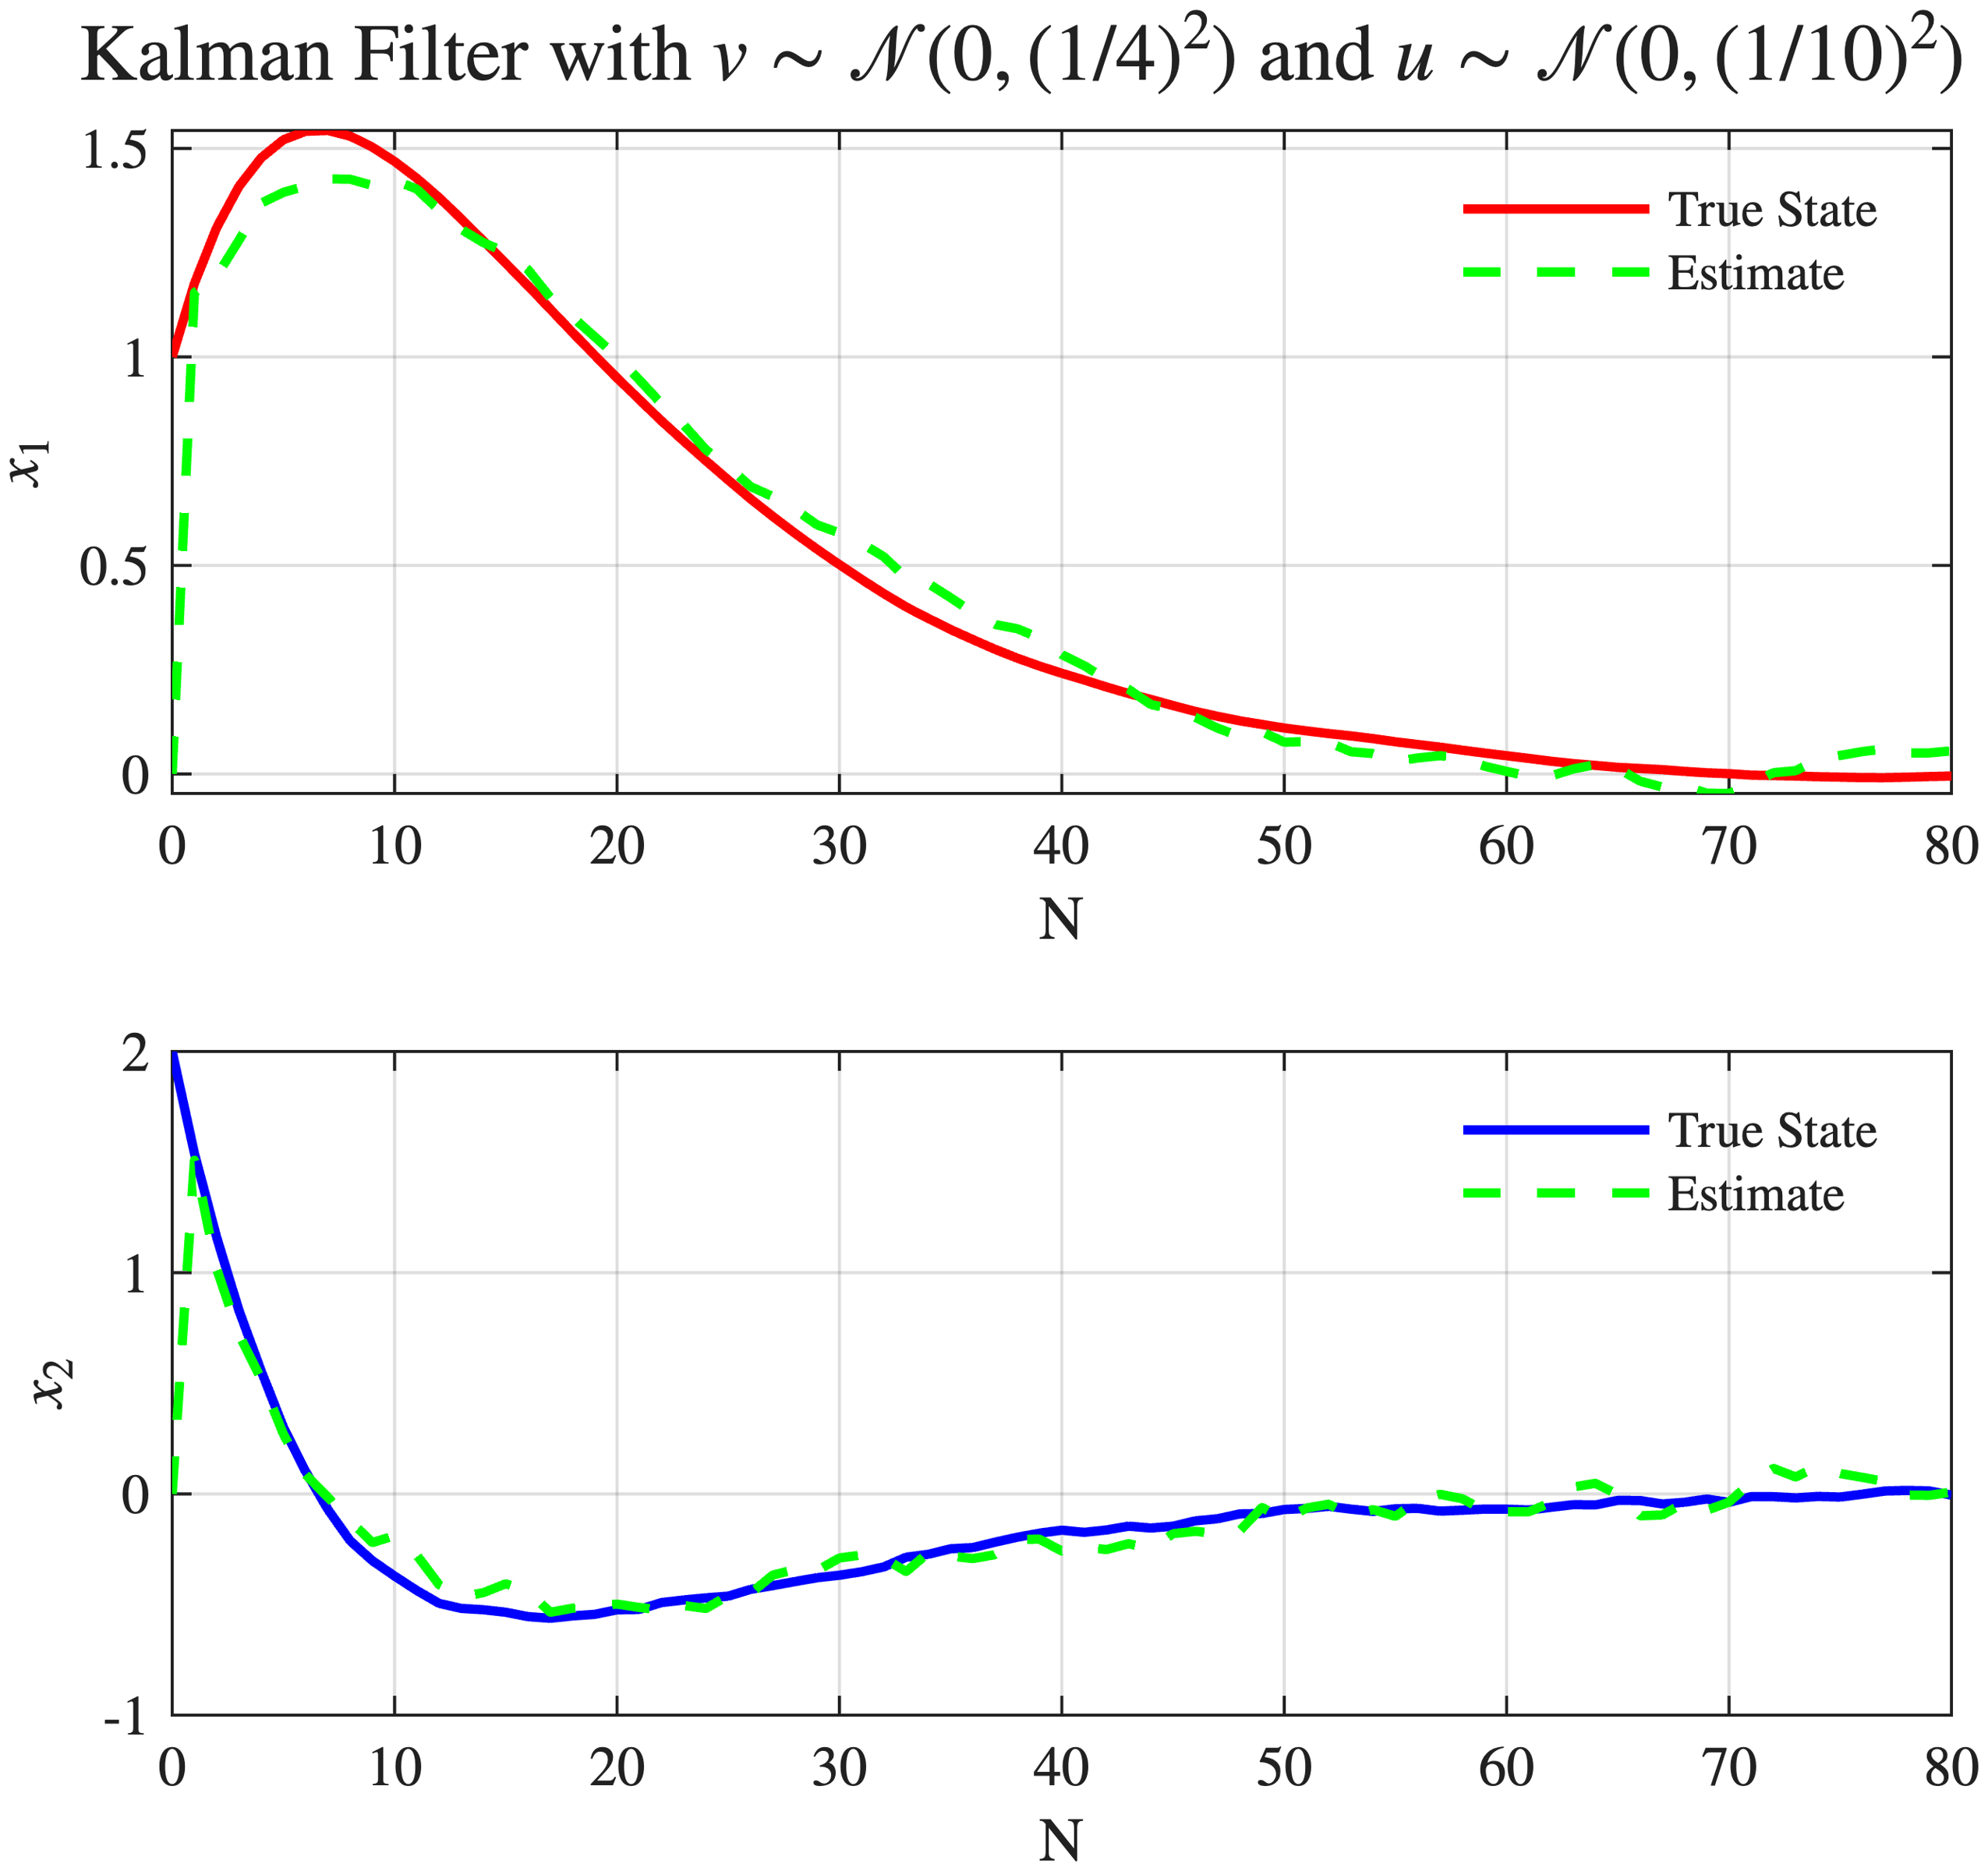
\includegraphics[width=.8\linewidth]{Images/KF_example1.png}
    \caption{True state of the system compared to the state estimate of the Kalman filter}
    \label{fig:kf full linear}
\end{figure}
\begin{figure}[ht]
    \centering
    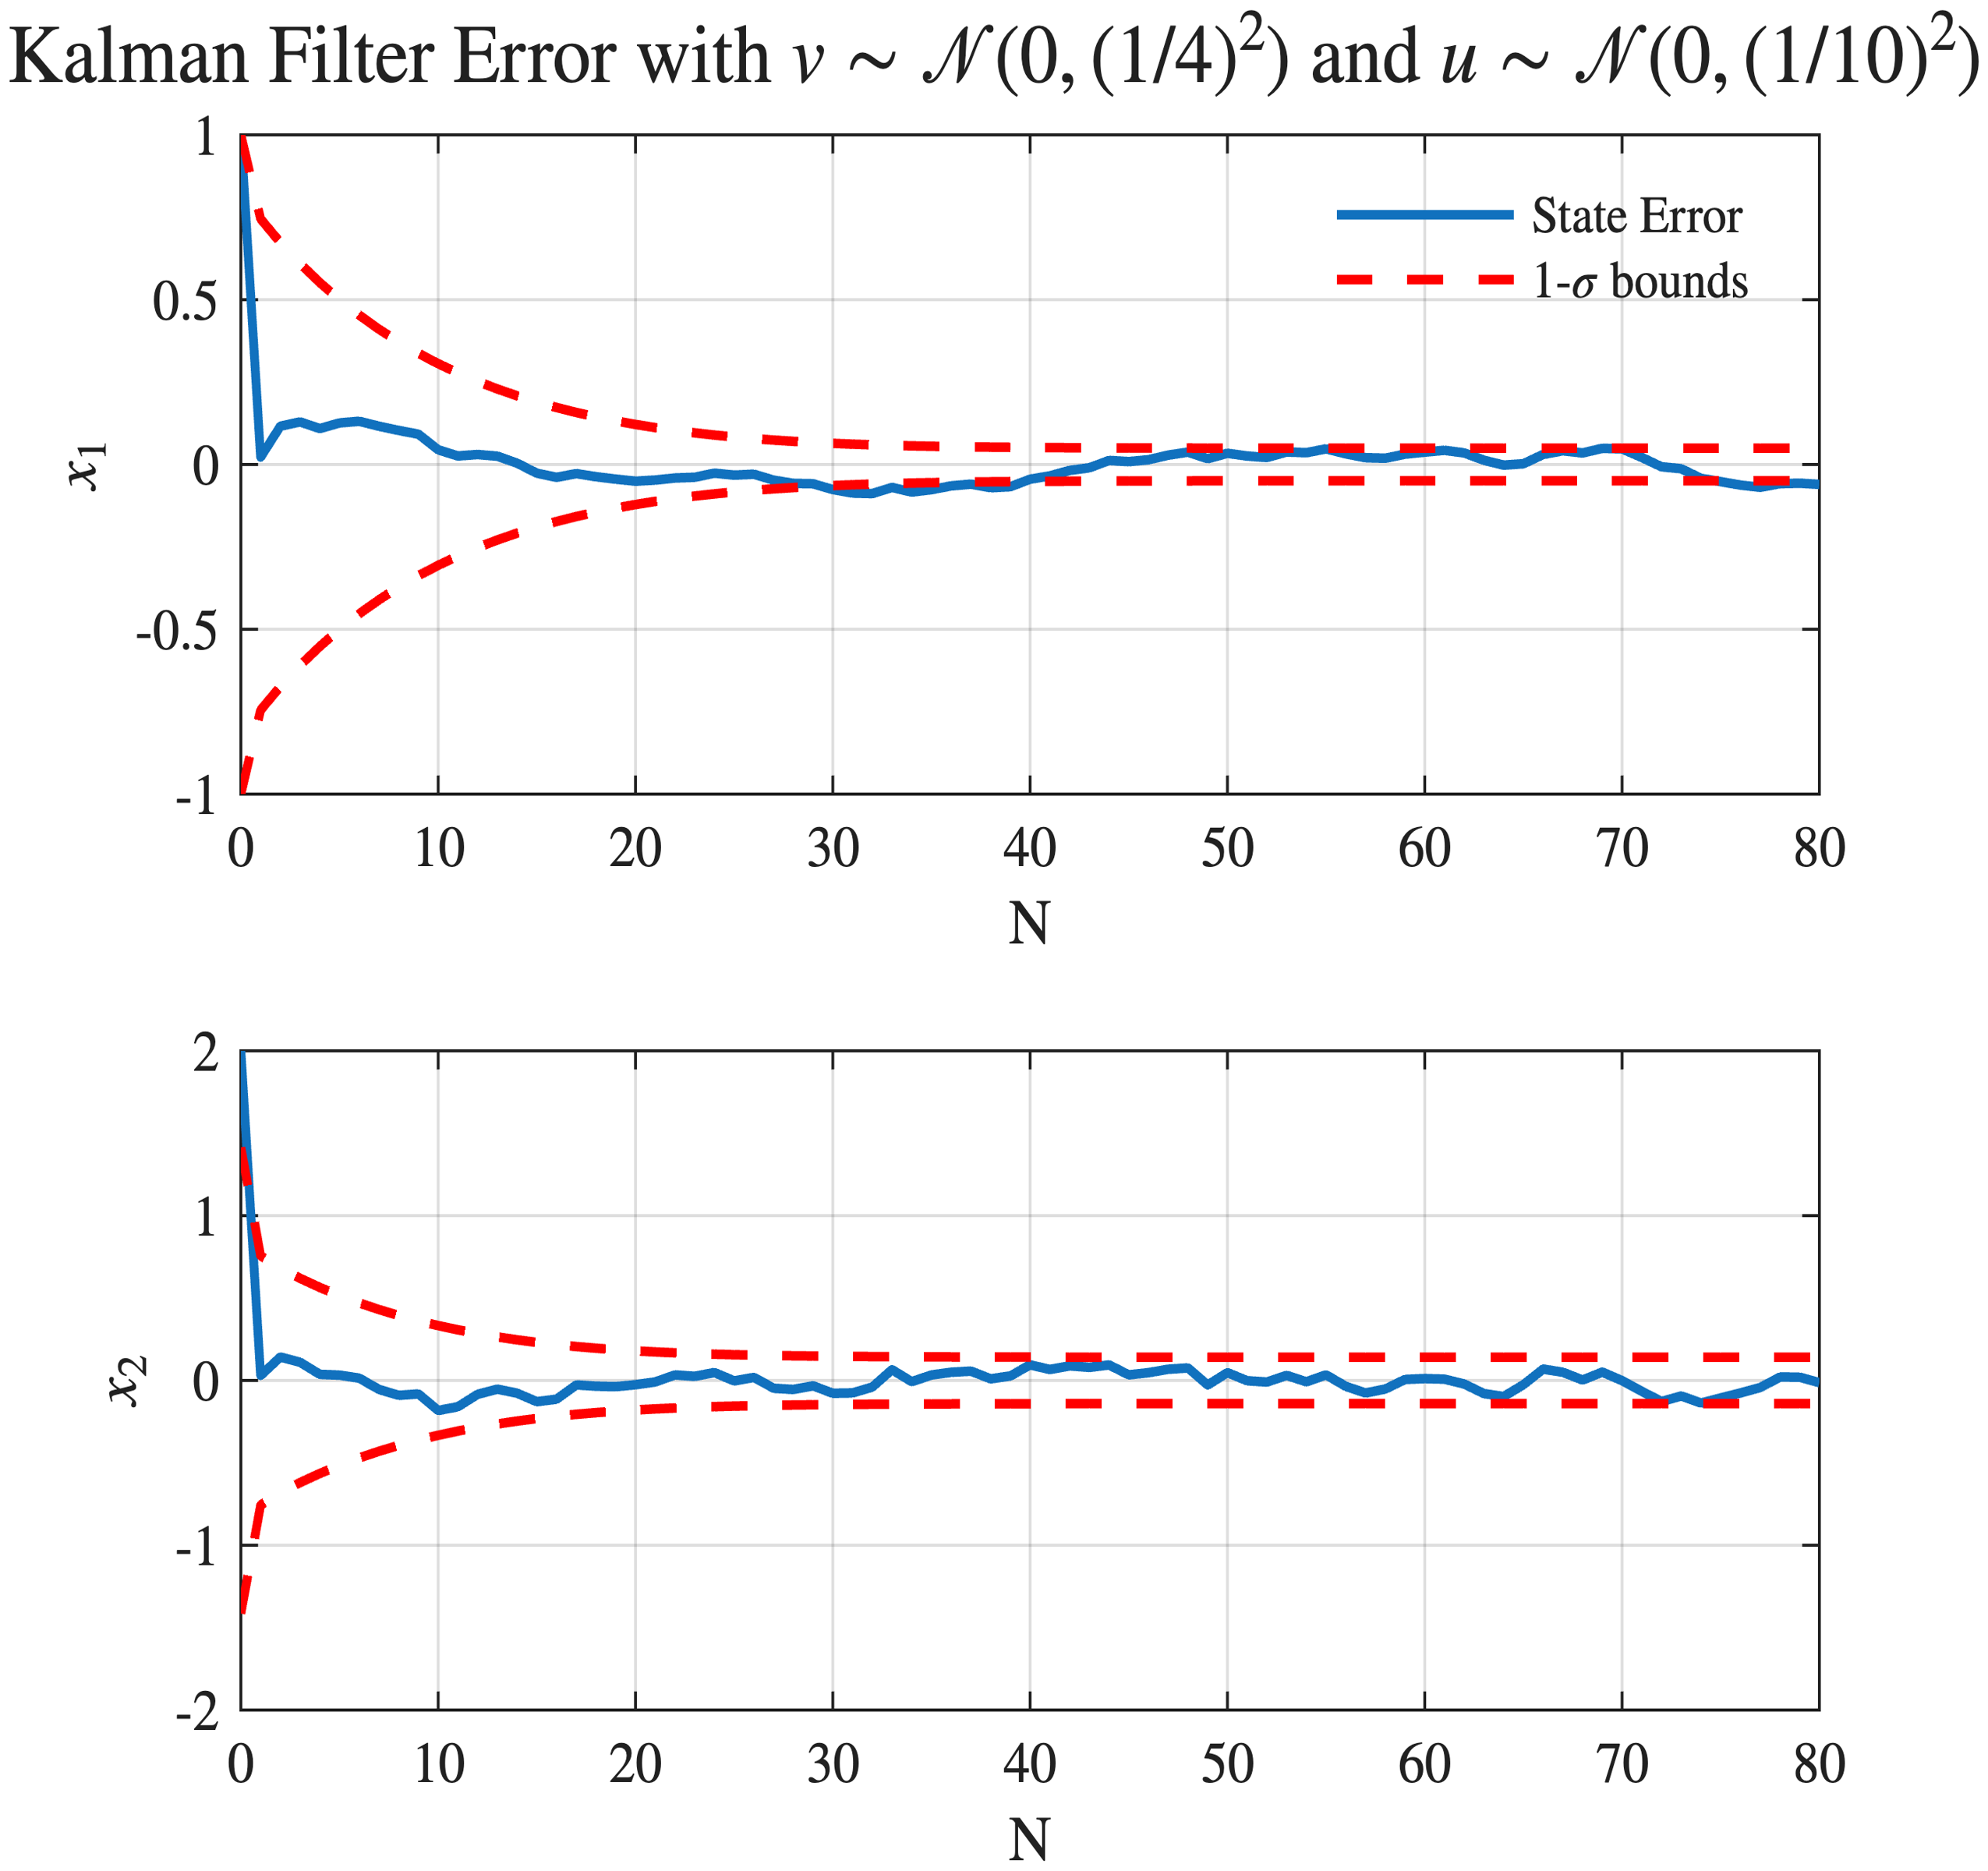
\includegraphics[width=.8\linewidth]{Images/KF_example2.png}
    \caption{Error in the state estimate of the Kalman filter with $1\sigma$ bounds (red dashed)}
    \label{fig:kf error linear}
\end{figure}
In typical analysis, we look at internal metrics of the filter because the true state of the system is not known. A common system metric is the measurement innovation of the filter at each step.


\subsubsection{Steady State Kalman Filtering}
For this problem, we will create a steady state filter for the discrete time system in the problem above to see the difference in performance (both computationally and in terms of filter outcomes). Since our state space is the same as the previous problem, we will only show the additions to the code. First, we establish the steady state Kalman gain of the system:
\begin{matlabscript}{}
% compute the steady state filter error covariance and Observer gain:
P = idare(Phi', C', B*B', D*D', [], []);
L = Phi*P*C'/(C*P*C' + D*D');
\end{matlabscript}
The loop for the computation of the new state estimate will be:
\begin{matlabscript}{}
% loop for KF:
for idx=1:z
    % calculate the true state:
    xn_1 = Phi*xn + B*w(idx);

    % calculate the meas:
    yn = C*xn + D*v(idx);

    % steady state KF:
    x_hat_n_1_steady  = (Phi-L*C)*x_hat_n_steady+L*yn;

    % save vars for plot
    x_hat_steady(idx,:) = x_hat_n_steady;

    % update vars for next step
    x_hat_n_steady = x_hat_n_1_steady;
    xn = xn_1;

end
\end{matlabscript}

We can compare the estimate of the steady state filter against the standard filter to see the difference. This is shown in \autoref{fig:steady}. We notice that the two estimates eventually become very close, with the steady state filter showing a different transient in the first 20-30 time steps. This result tells us that a good initial condition for $\bm{x}_0$ is more important for the steady state filter, as the transient response is fixed by the eigenvalues of $\Phi-LC$. Since the non steady filter can change the Kalman gain, convergence is often faster when initial conditions are unknown.
\begin{figure}[ht]
    \centering
    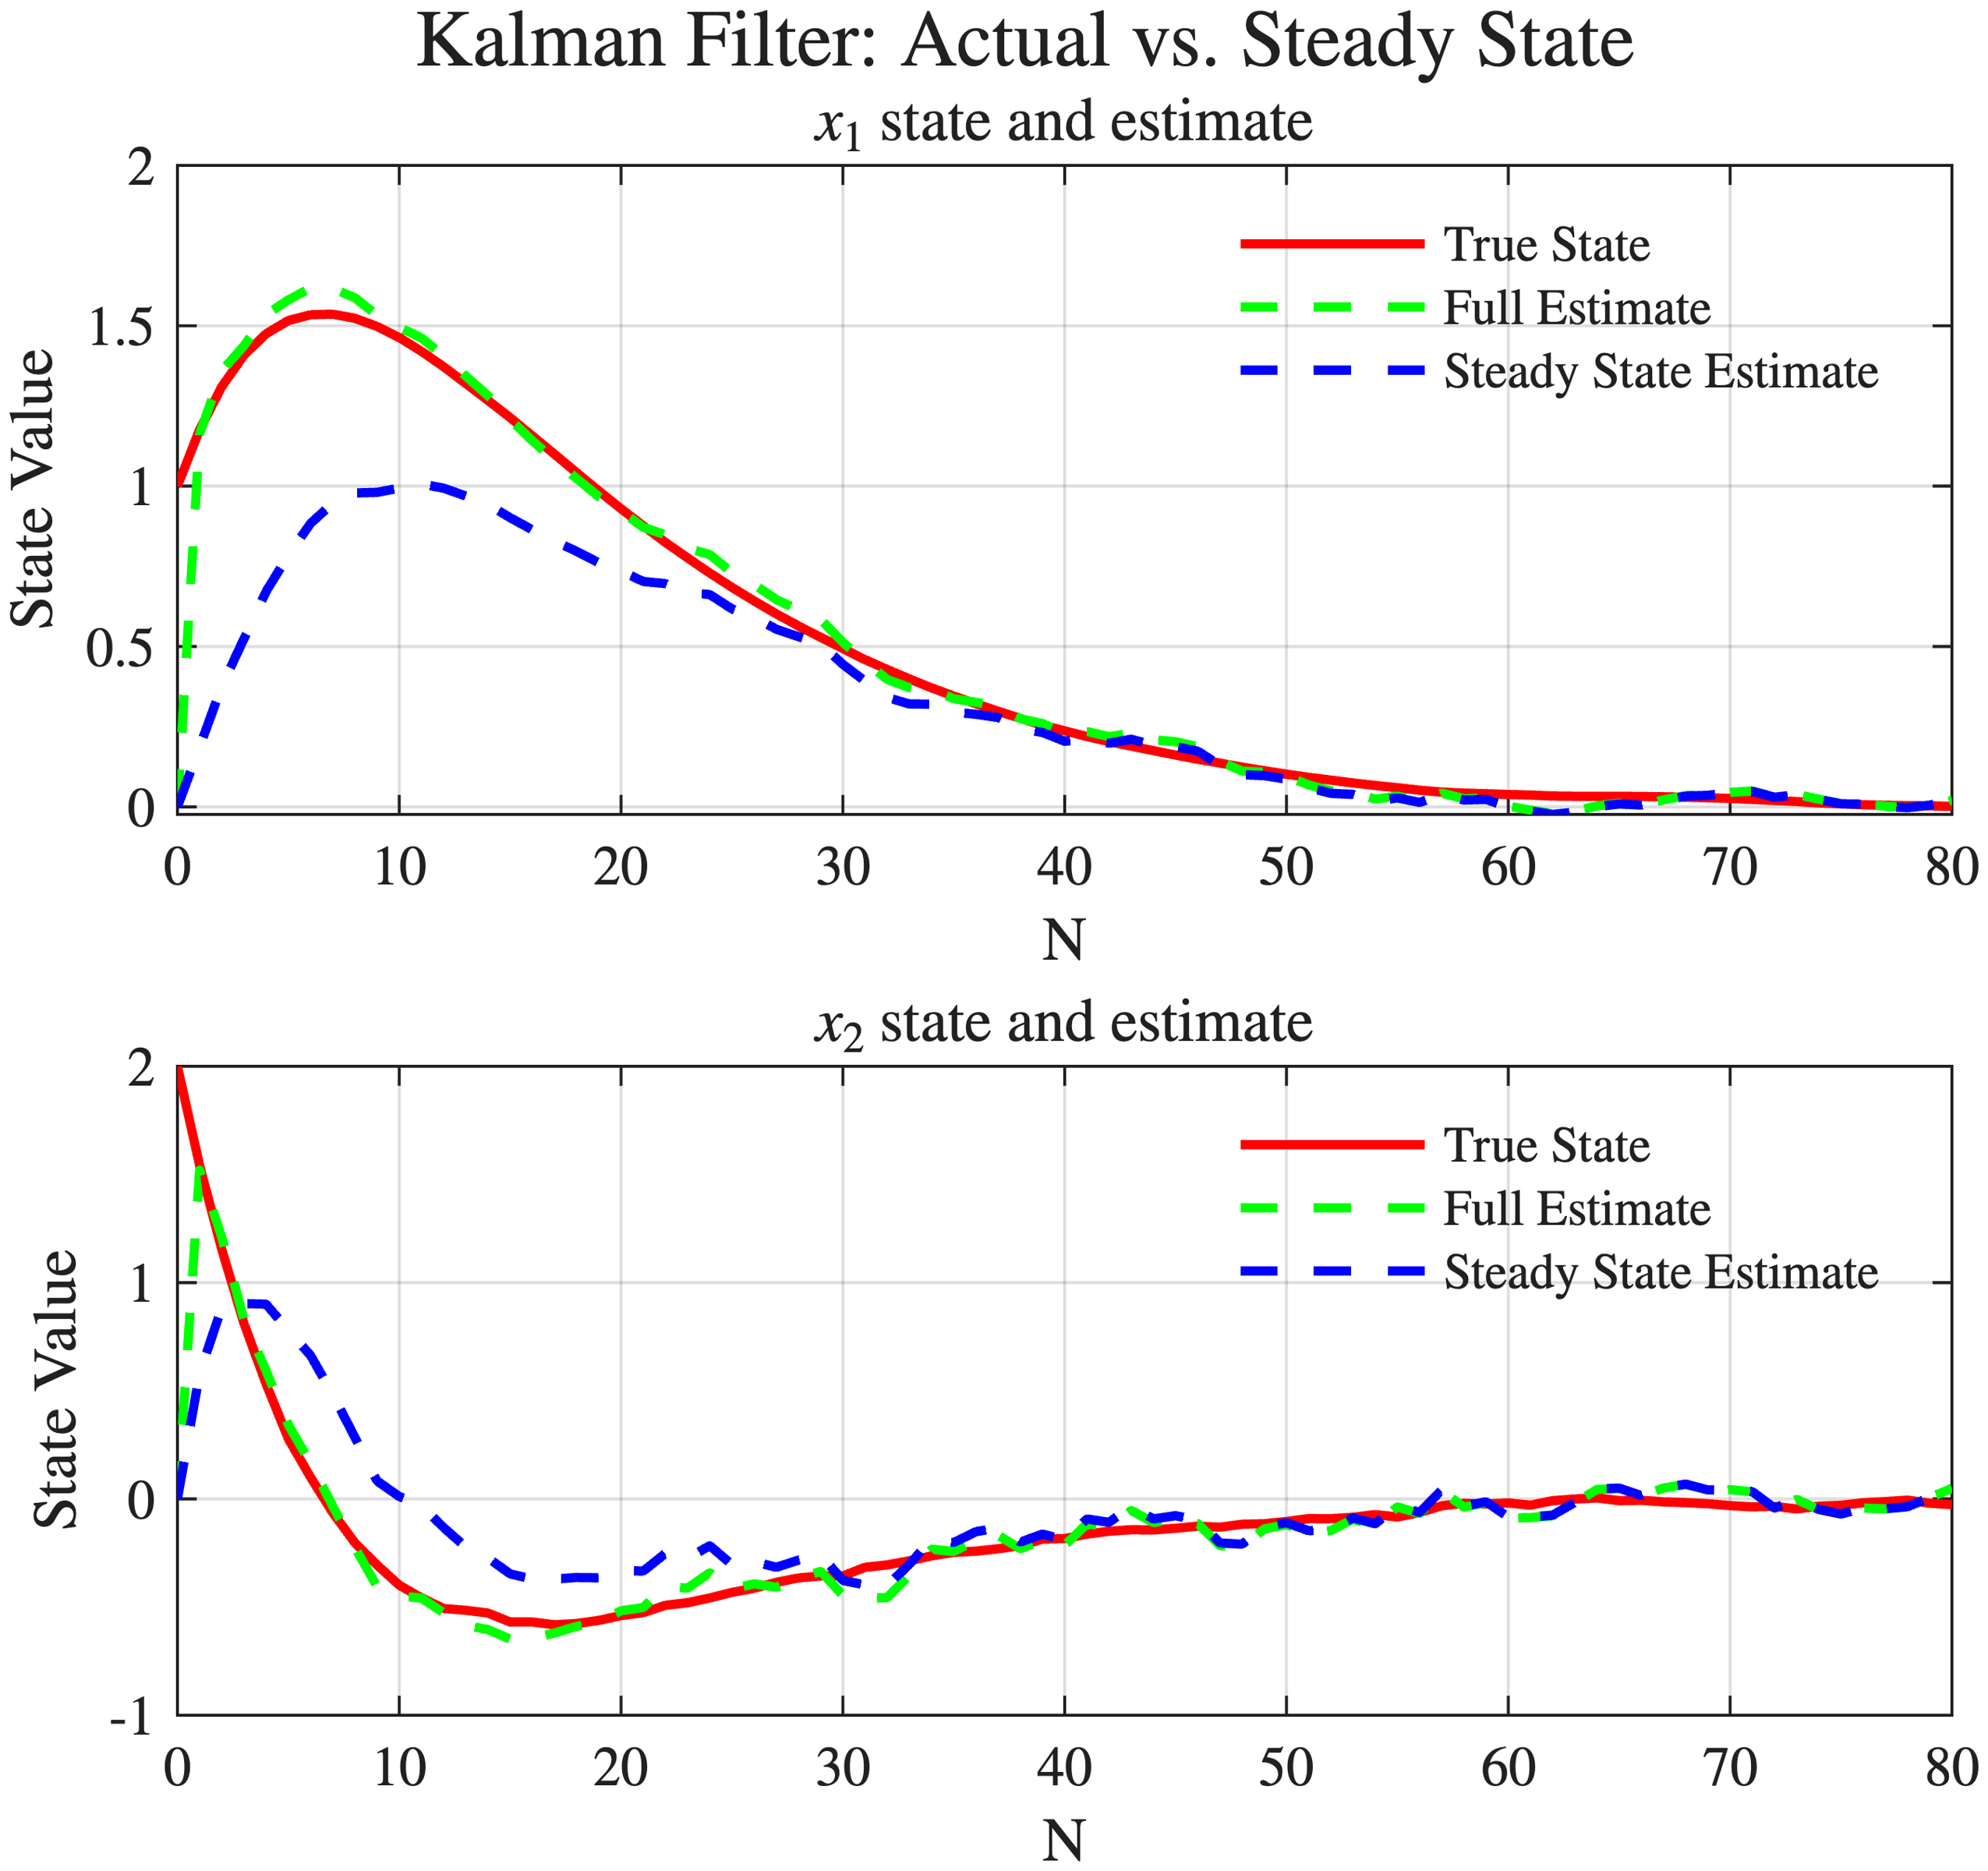
\includegraphics[width=1\linewidth]{SteadyFilter.png}
    \caption{Comparison of standard Kalman filter with the steady state Kalman filter}
    \label{fig:steady}
\end{figure}
For this $2\times2$ state space, the steady state filter computes its estimate in roughly one half to one third the time of the standard Kalman filter in MATLAB. Larger state spaces will benefit much more from the precomputation. Altogether, matrix inversions and multiplications in the standard filter create $\mathcal{O}(n^3+m^3)$ operations at each step (where $n$ is the size of the state $\bm{x}$ and $m$ the size of the measurement). For the steady state filter, we only need matrix multiplication and has time complexity of $\mathcal{O}(n^2+nm)$. We will see even greater improvements as the matrices become larger.


\subsubsection{Steady State Kalman Filtering with Control (Simulink)}


\newpage
\printendnotes


\chapter{Extensions of Kalman Filtering}\label{chap:kalman filter extensions}
In the development of the optimal estimator which resulted in the Kalman filter, we have made quite a few assumptions, some of which are quite limiting to its use. First and foremost is the assumption that our system must be linear. This, as it turns out, is the most egregious of the assumptions in the Kalman filter which most different approaches seek to resolve. There are several methods by which this can be resolved, each of which generates a variation of the Kalman filter with greater applicability to nonlinear systems. 

There are quite a few options to choose here, each with certain benefits and drawbacks for certain applications. Recent work has tended to favor the \gls{ukf} (\cite{wan_unscented_2000, chadha_unscented_2019}), but to understand that approach we must first look at the \gls{ekf} and related approaches.

There are other methods by which the state estimation can be achieved that are not related to the Kalman filter, such as the particle filter. While these can be quite useful, they fall outside the scope of this book and will not be discussed here.

To make this book practical, I want to provide real examples of each of these types of filters in MATLAB. Many times, there is a large gap between the practical application of these filters and the theory behind them. Although MATLAB has some built-in functionality for Kalman filtering, each situation -- particularly with the \gls{ekf} and \gls{ukf} -- can be quite unique and require a specialized implementation. It is best then, to understand code logic rather than being reliant on built-in functionality.

\section{The Extended Kalman Filter}

The \gls{ekf} is the first major extension of the Kalman filter.  In the \gls{ekf}, we use the concept of linearization in order to approximate a non-linear system as linear. In this way, we can apply the principles of Kalman filtering to a non-linear problem. At each point along our trajectory, we will linearize the dynamics of the system in order to propagate the state and the covariance. When we recieve measurement updates


\begin{example}[The 1D Radar Problem (Gelb)]
Do this later
\end{example}

\section{Trajectory Linearization}
One method that can be used that is less computationally expensive than the full \gls{ekf} is a method of `trajectory linearization'. This simplification may be used when we have prior information about the trajectory of the object. 

In this approach, we first construct a reference trajectory and apply linearization about the reference trajectory. Then, at every point in time, the reference trajectory linearization can be used for the kalman filter.

As an example, if we have some \gls{imu} data, we may propagate that data under the assumption that is perfect. This will give us a trajectory which is not perfect, but is good enough that it can inform our linearization model. We take a linearization at each point of this trajectory, and then we only have to match the result of the Kalman filter to this reference trajectory at each time.




\section{Multiplicative Kalman Filter}
The multiplicative Kalman filter is a special variety of the Kalman filter which is appropriate for systems which are non-linear but have a manifold description which is easily classified in terms of their \gls{lie algebra}. Often, rotations use the multiplicative Kalman filter because they fit this description exactly.

To see why we need the multiplicative Kalman filter, let us consider the problem of estimating the quaternion representation of the attitude of a vehicle. Our measurement update may look like:
$$\bm{q}^+=\bm{q}^-+K[\bm{y}-H\bm{q}^-]$$
One problem that can immediately be seen with this approach is that there is no enforcement of the quaternion magnitude. If the attitude errors are quite large, this can be quite a problem, and the enforcement of the quaternion magnitude needs to be performed elsewhere. This leads to the quaternion error update being less optimal than it otherwise would be.

One solution to counter this is to introduce a \textit{multiplicative} approach to the Kalman filter. Such an approach would maintain the quaternion magnitude constraint and prove useful in other parameterizations of the attitude representation.

\section{The Unscented Kalman Filter}
The unscented Kalman filter is another extension of the Kalman filter which is particularly useful in modeling systems which are highly non-linear in nature. The basic idea of the unscented Kalman filter is to make estimates for how the mean and covariance of the system change under the nonlinear dynamics of the system. If we are smart and pick a few points that model the distribution of the system well, we can track their evolution and reconstruct the change in the distribution.

The unscented Kalman filter relies on our knowledge used in deriving the Kalman filter. Let's briefly review the basics to see how we can implement them when our system is nonlinear.

Let's remember that we were able to define our state estimate in terms of the $R$ matrices as follows:
$$\bm{\hat{x}}=\mathcal{P}_\mathcal{M}\bm{x}=R_{xg}R_g^{-1}g$$
Here, we're going to define our $g$ as the following column vector:
$$g=\begin{bmatrix}
    1\\y-\mu_y
\end{bmatrix}$$
We can apply the standard formula for the state estimate. Let's first compute $R_g$:
$$R_g=\mathbb{E}gg^*=\mathbb{E}\begin{bmatrix}
1&y-\mu_y\\y-\mu_y&(y-\mu_y)^2
\end{bmatrix}=\begin{bmatrix}
    1&0\\0&\mathrm{Var}(y)
\end{bmatrix}$$
Now we compute $R_{xg}$:
$$R_{xg}=\mathbb{E}xg^*=\mathbb{E}x\begin{bmatrix}
    1&y-\mu_y
\end{bmatrix}=\begin{bmatrix}
    \mu_x&\text{Cov(x,y)}
\end{bmatrix}$$
If we multiply all these elements together, we will find that our state estimate is the following:
$$\bm{\hat{x}}=\begin{bmatrix}
    \mu_x&\text{Cov(x,y)}
\end{bmatrix}\begin{bmatrix}
    1&0\\0& \frac{1}{\mathrm{Var}(y)}
\end{bmatrix}\begin{bmatrix}
    1\\y-\mu_y
\end{bmatrix}=\mu_x+\frac{\text{Cov}(x,y)}{\text{Var}(y)}(y-\mu_y)$$
This form gives us an explicit connection between the $R$ matrices and the statistical values of the variance, covariance, and mean. If we can estimate each of these quantities, we can come up with a state estimate for our system.

\begin{exercise}
Remember that the error for a system is defined as:
$$e^2=\mathbb{E}(\bm{x}-\bm{\hat{x}})(\bm{x}-\bm{\hat{x}})^*=R_x-R_{xg}R_g^{-1}R_{xg^*}$$
Show that this can be written in terms fo the variance and covariance as:
$$e^2=\text{Var}(x)-\text{Cov}(x,y)\text{Var}(y)^{-1}\text{Cov}(y,x)$$
\end{exercise}

\subsection{The Unscented Transform}

\subsection{The Unscented Kalman Filter Algorithm}

\subsection{Examples of the UKF}

\newpage
\printendnotes



\chapter{Case Study: Inverted Pendulum}\label{chap:inverted pendulum}
The inverted pendulum is a classic problem in control theory, and for good reason! It demonstrates all of the basics of control theory, from derivation of \glspl{eom}, system linearization, and control design. With this problem, we can show a definitive example of many of the previous topics of discussion with a real application.

\begin{figure}[H]
    \centering
    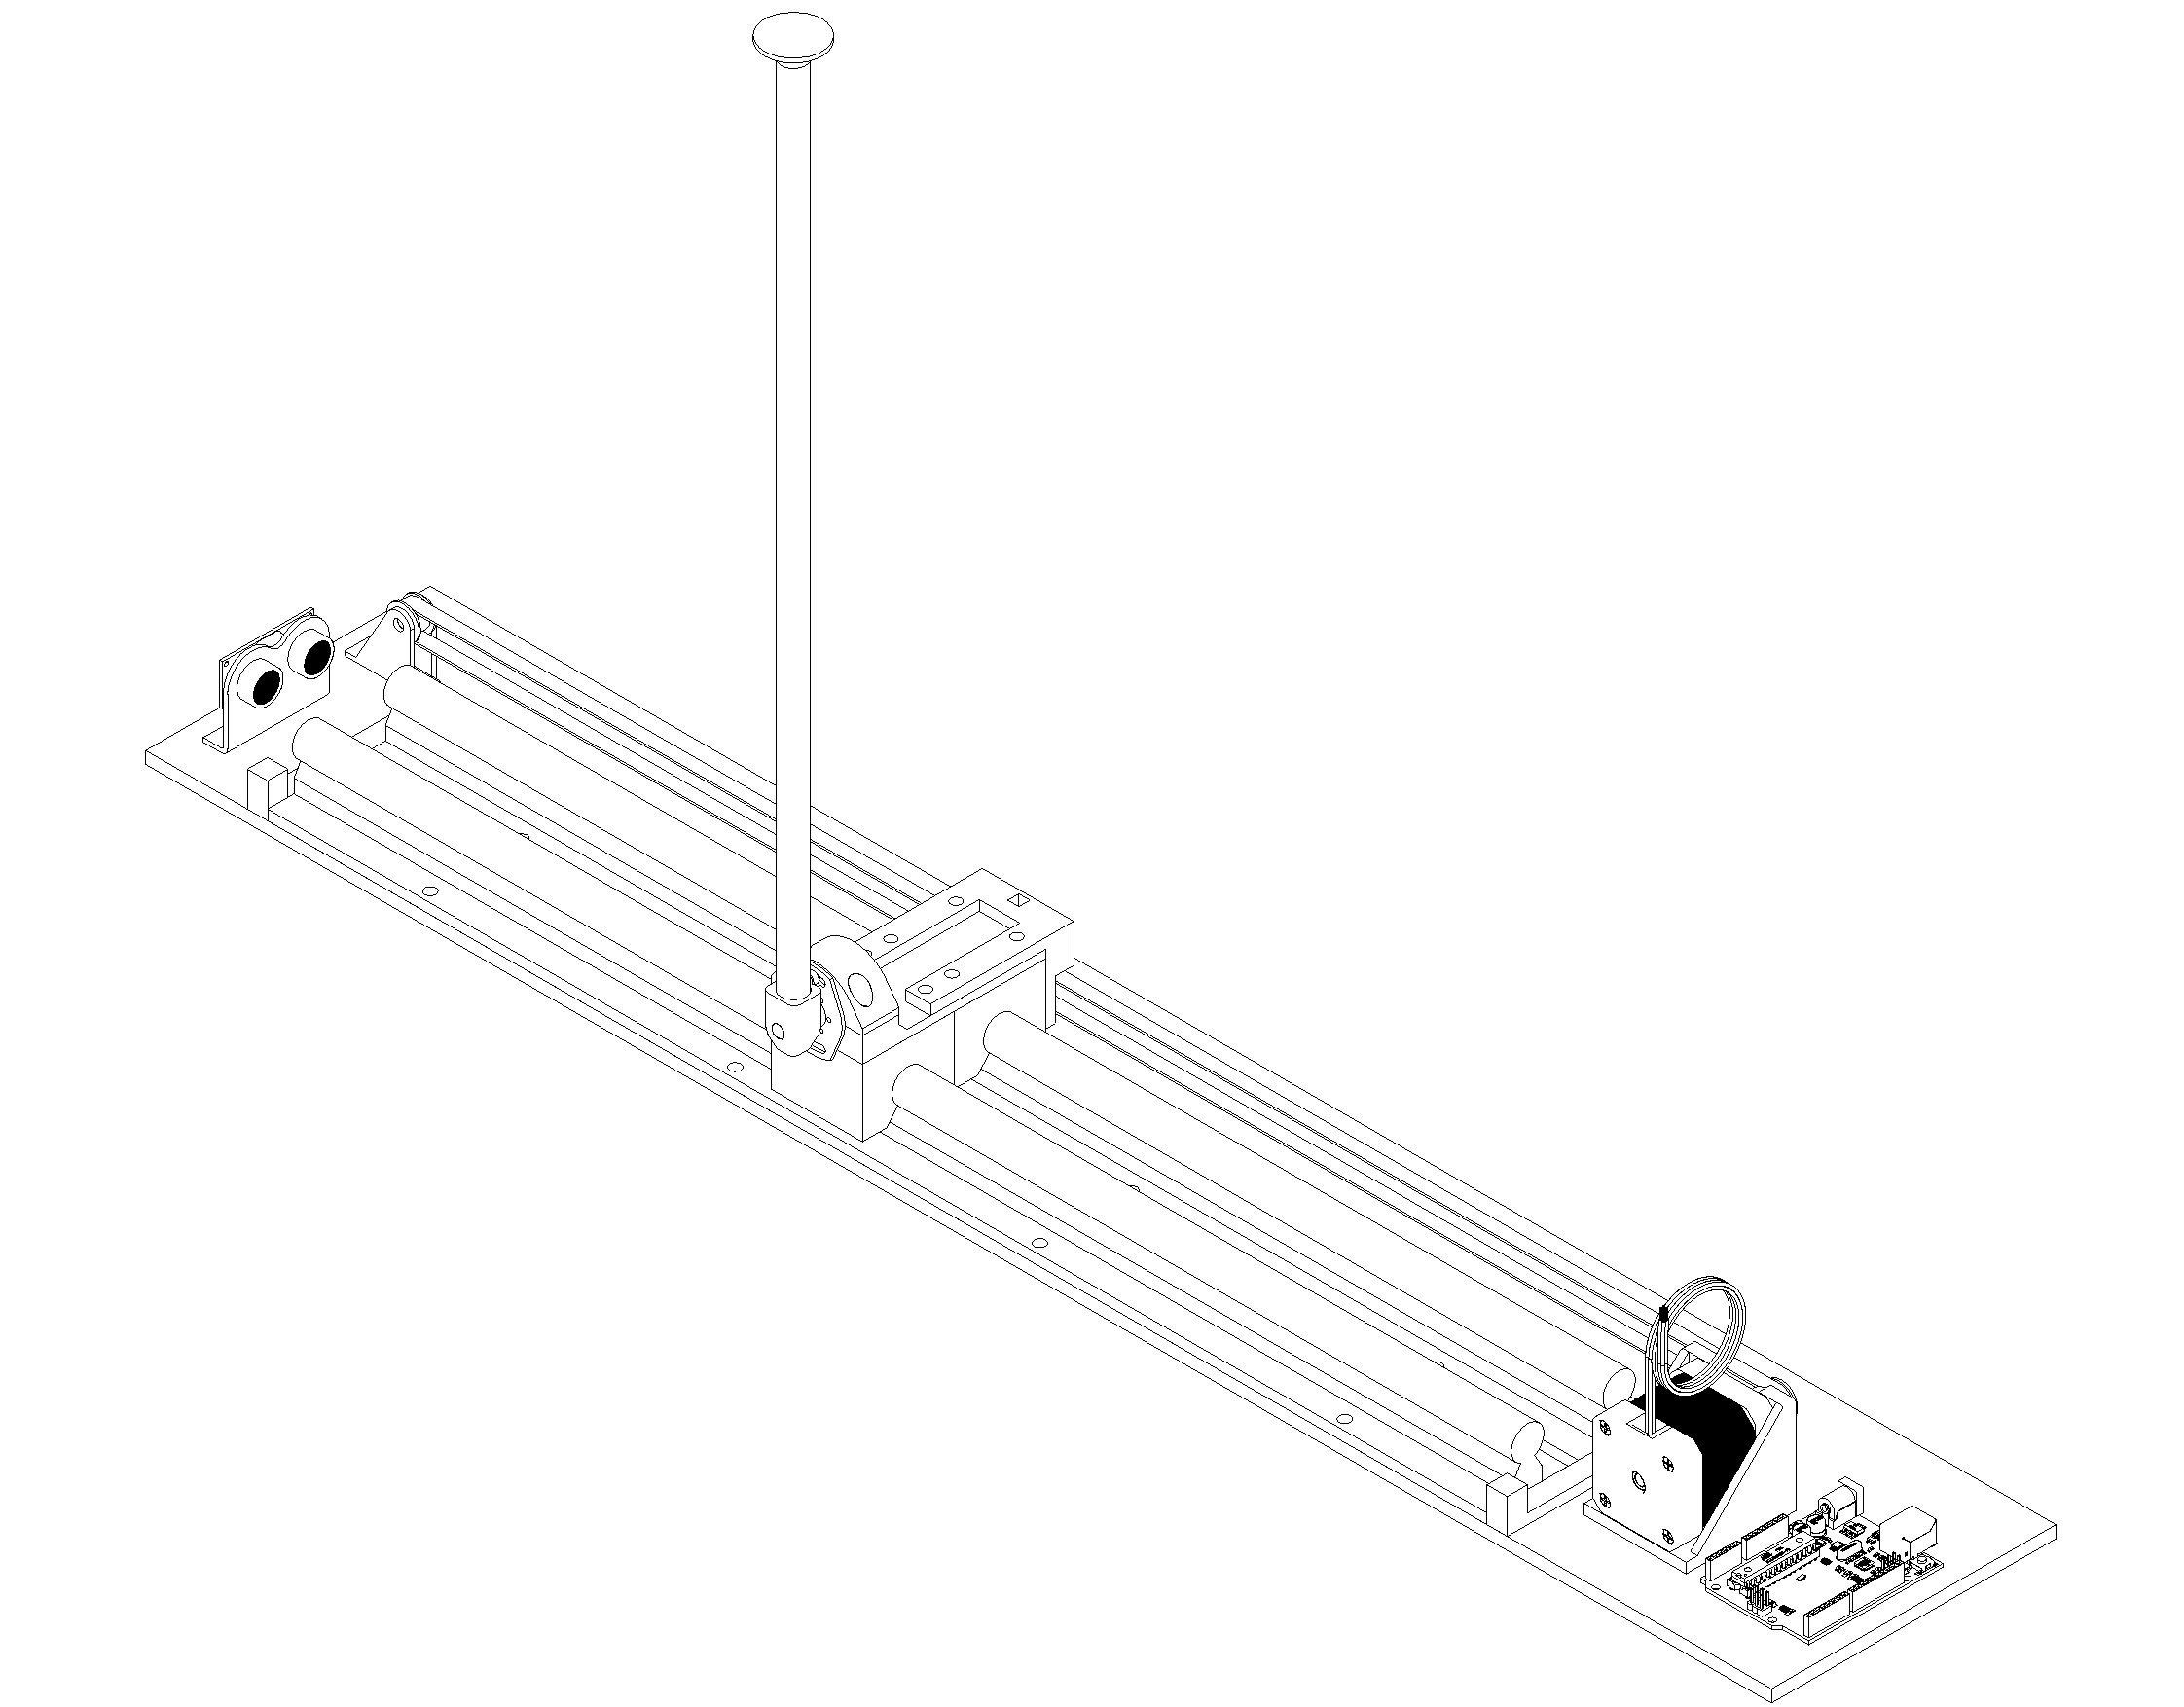
\includegraphics[width=.9\linewidth]{Images/InvertedPendulum.pdf}
    \caption{The Inverted Pendulum}
    \label{fig:inverted pend}
\end{figure}

At the end of this chapter, we will apply this controller to a real inverted pendulum system that I have built. My hope is that this will help demonstrate both the theory and practical application of the control theory concepts covered thus far. Additionally, some practical control applications will be discussed, such as the speed and torque control of DC motors.

\section{Equations of Motion}\label{sec:pend eom}
For any control system, we must understand the dynamics of the system that we want to control. For the simple inverted pendulum, this is quite easy to derive using energy mechanics.

Here, I will choose to use the \gls{Lagrangian} approach in the derivation, although the \gls{Hamiltonian} or Newtonian approach can also be taken. For this particular system, the \gls{Lagrangian} approach is quite simple and requires less knowledge of the forces acting on the system, which can become quite complicated! 

\subsubsection{Lagrangian Formulation}

We will consider a simple version of the pendulum-cart system, as shown in \autoref{fig:Pendulum Cart}.

\begin{figure}[ht]
    \centering



\tikzset{every picture/.style={line width=0.75pt}} %set default line width to 0.75pt        

\begin{tikzpicture}[x=0.75pt,y=0.75pt,yscale=-1,xscale=1]
%uncomment if require: \path (0,300); %set diagram left start at 0, and has height of 300

%Shape: Rectangle [id:dp1823165404229382] 
\draw   (244.27,180) .. controls (244.27,174.48) and (248.75,170) .. (254.27,170) -- (374.27,170) .. controls (379.8,170) and (384.27,174.48) .. (384.27,180) -- (384.27,219.09) .. controls (384.27,224.61) and (379.8,229.09) .. (374.27,229.09) -- (254.27,229.09) .. controls (248.75,229.09) and (244.27,224.61) .. (244.27,219.09) -- cycle ;
%Straight Lines [id:da7877170508964265] 
\draw [line width=2.25]    (270,70) -- (314.27,199.55) ;
\draw [shift={(314.27,199.55)}, rotate = 71.13] [color={rgb, 255:red, 0; green, 0; blue, 0 }  ][fill={rgb, 255:red, 0; green, 0; blue, 0 }  ][line width=2.25]      (0, 0) circle [x radius= 2.14, y radius= 2.14]   ;
%Straight Lines [id:da5998055377665403] 
\draw    (363.64,200) -- (437,200) ;
\draw [shift={(440,200)}, rotate = 180] [fill={rgb, 255:red, 0; green, 0; blue, 0 }  ][line width=0.08]  [draw opacity=0] (8.93,-4.29) -- (0,0) -- (8.93,4.29) -- cycle    ;
%Shape: Arc [id:dp2580429075144265] 
\draw  [draw opacity=0] (287.33,119.03) .. controls (295.78,116.12) and (304.84,114.55) .. (314.27,114.55) -- (314.27,197.27) -- cycle ; \draw [color={rgb, 255:red, 74; green, 144; blue, 226 }  ,draw opacity=1 ]   (290.27,118.08) .. controls (297.87,115.78) and (305.93,114.55) .. (314.27,114.55) ; \draw [shift={(314.27,114.55)}, rotate = 180] [color={rgb, 255:red, 74; green, 144; blue, 226 }  ,draw opacity=1 ][line width=0.75]    (0,5.03) -- (0,-5.03)   ; \draw [shift={(287.33,119.03)}, rotate = 341] [fill={rgb, 255:red, 74; green, 144; blue, 226 }  ,fill opacity=1 ][line width=0.08]  [draw opacity=0] (8.04,-3.86) -- (0,0) -- (8.04,3.86) -- cycle    ;
%Shape: Circle [id:dp15264344475000924] 
\draw   (260,239) .. controls (260,233.48) and (264.48,229) .. (270,229) .. controls (275.52,229) and (280,233.48) .. (280,239) .. controls (280,244.52) and (275.52,249) .. (270,249) .. controls (264.48,249) and (260,244.52) .. (260,239) -- cycle ;
%Shape: Circle [id:dp05286140767854186] 
\draw   (350,239) .. controls (350,233.48) and (354.48,229) .. (360,229) .. controls (365.52,229) and (370,233.48) .. (370,239) .. controls (370,244.52) and (365.52,249) .. (360,249) .. controls (354.48,249) and (350,244.52) .. (350,239) -- cycle ;
%Straight Lines [id:da14376683390655187] 
\draw [color={rgb, 255:red, 74; green, 144; blue, 226 }  ,draw opacity=1 ] [dash pattern={on 4.5pt off 4.5pt}]  (160,200) -- (230,200) ;
%Straight Lines [id:da36211983725754393] 
\draw    (259,74) -- (303.27,203.55) ;
\draw [shift={(303.27,203.55)}, rotate = 251.13] [color={rgb, 255:red, 0; green, 0; blue, 0 }  ][line width=0.75]    (0,5.59) -- (0,-5.59)   ;
\draw [shift={(259,74)}, rotate = 251.13] [color={rgb, 255:red, 0; green, 0; blue, 0 }  ][line width=0.75]    (0,5.59) -- (0,-5.59)   ;

% Text Node
\draw (445,187.4) node [anchor=north west][inner sep=0.75pt]    {$\dot{x}$};
% Text Node
\draw (297,92.4) node [anchor=north west][inner sep=0.75pt]  [font=\normalsize,color={rgb, 255:red, 74; green, 144; blue, 226 }  ,opacity=1 ]  {$\theta $};
% Text Node
\draw (107,190.4) node [anchor=north west][inner sep=0.75pt]  [color={rgb, 255:red, 74; green, 144; blue, 226 }  ,opacity=1 ]  {$V=0$};
% Text Node
\draw (314.27,205.95) node [anchor=north] [inner sep=0.75pt]    {$M$};
% Text Node
\draw (272,52.4) node [anchor=north] [inner sep=0.75pt]    {$m$};
% Text Node
\draw (263,128.4) node [anchor=north west][inner sep=0.75pt]    {${l}$};

\end{tikzpicture}

    \caption{Pendulum-Cart System}
    \label{fig:Pendulum Cart}
\end{figure}
In this depiction, we will make quite a few simplifying assumptions, although some of these excluded dynamics can quite easily be recovered with a little effort:
\begin{itemize}
    \item The pendulum arm is assumed to originate at the center of mass of the cart.
    \item Friction and damping in the system is neglected, both in the rotation of the arm and the movement of the cart
    \item The reference for the potential energy is placed at the center of mass of the cart.
\end{itemize}

With these assumptions in place, we can apply the methods of \gls{Lagrangian} mechanics to derive the \glspl{eom} of the system. 

Starting with the \gls{Lagrangian} itself, we first define the generalized coordinates to use. In this case, the selection of $x$ and $\theta$ is quite obvious, as these two provide a minimal and simple realization of the system.

Since the motion of the system is non-obvious, it is best to employ the generalized equation for the kinetic energy in the derivation:
$$T=\frac{1}{2}\sum_im_i\left(\sum_j\frac{\partial\vec{r}_i}{\partial q_j}\dot{q}_j+\frac{\partial \vec{r}_i}{\partial t}\right)^2$$
There are two masses in the system, so the sum over $i$ includes both. We define the kinetic energy of the system as the sum of the kinetic energies of the cart ($i=1)$ and the pendulum ($i=2$). For the cart, only linear motion is permitted, so the kinetic energy is:
$$T_{cart}=\frac{1}{2}M\dot{x}^2$$
For the pendulum arm, both translational and rotational motion is permitted, so the total kinetic energy is more complicated. We will employ the formula above to find the kinetic energy in this case, considering only $i=2$ since $i=1$ has just been solved:
$$T_{pend}=\frac{1}{2}m\left(\sum_j\frac{\partial\vec{r}_2}{\partial q_j}\dot{q}_j+\frac{\partial \vec{r}_2}{\partial t}\right)^2$$
The vector $\vec{r}_2$ is expressed in terms of the two generalized coordinates, which gives 
$$\vec{r}_2=(x+l\sin\theta)\hat{\imath}+(l\cos\theta)\hat{\jmath}$$
One `trick' we can do in the computation that is sometimes simpler is to unexpand the chain rule and express the kinetic energy as:
$$T_{pend}=\frac{1}{2}m|\dot{r}_2|^2$$
Computing the value of $\dot{r}_2$ (remembering the implicit chain rule, now that we are not explicitly writing it), we have:
$$\dot{r}_2=(\dot{x}+l\cos\theta\dot{\theta})\hat{\imath}+(-l\sin\theta\dot{\theta})\hat{\jmath}$$
Performing the norm-square of $\dot{r}_2$ is the same as the dot product, so we square each element:
$$T_{pend}=\frac{1}{2}m\left[(\dot{x}+l\cos\theta\dot{\theta})^2+(-l\sin\theta\dot{\theta})^2\right]$$
Importantly, the computation of this gives a cross term from the expansion of the first term, which we may have missed otherwise. Altogether, $T_{pend}$ is:
$$T_{pend}=\frac{1}{2}m\dot{x}^2+\frac{1}{2}ml^2\dot{\theta}^2+ml\cos\theta\dot\theta\dot{x}$$
At this point, we can identify that the term $\frac{1}{2}ml^2\dot{\theta}^2$ is exactly the rotational kinetic energy of the rod. As a result, we can replace this term with $\frac{1}{2}I\dot{\theta}^2$. Finally, summing the two values of $i$ gives us the following kinetic energy for the system:
$$T_{cart}+T_{pend}=\frac{1}{2}\left[\left(M+m\right)\dot{x}^2+I\dot{\theta}^2\right]+ml\cos\theta\dot{\theta}\dot{x}$$

The potential is quite easy. For the cart, no potential exists because we have defined the potential at the center of mass to be $0$. For the arm, the potential is dependent on the angle, with the relationship given by:
$$V_{pend}=mgl\cos{\theta}$$
Altogether, this gives a \gls{Lagrangian} of the system as:
$$L=\frac{1}{2}\left[\left(M+m\right)\dot{x}^2+I\dot{\theta}^2\right]+ml\cos\theta\dot{\theta}\dot{x}-mgl\cos{\theta}$$
From here, we simply apply the Euler-Lagrange equations in both the $x$ and $\theta$ component directions.
\subsubsection{EOM Derivation}
Starting with the $x$-direction, we can directly apply the Euler-Lagrange equation with a generalized force to find the solution:
$$\frac{d}{dt}\left(\frac{\partial L}{\partial \dot{x}}\right)=\frac{\partial L}{\partial x}+F$$
Since $x$ itself has no presence in the equation,  $x$ is a cyclic coordinate in the solution. This directly implies linear momentum in the system is conserved by Noether's Theorem when no actuating forces are present. Additionally, this implies the RHS of the equation must be $F$ only. Considering the LHS then, we have:
$$\frac{d}{dt}\left(\frac{\partial}{\partial \dot{x}}\frac{1}{2}\left[\left(M+m\right)\dot{x}^2+I\dot{\theta}^2\right]+ml\cos\theta\dot{\theta}\dot{x}-mgl\cos{\theta}\right)$$
This simplifies quite quickly upon evaluation of the partial derivative to:
$$\frac{d}{dt}\left[\left(M+m\right)\dot{x}+ml\cos\theta\dot\theta\right]=F$$
Which is quite simply:
$$(M+m)\ddot{x}+ml\cos\theta\ddot{\theta}-ml\sin\theta\dot{\theta}^2=F$$
Next, we consider the $\theta$ component, which is quite a bit simpler. There is no generalized force in this component direction, so the result is:
$$\frac{d}{dt}\left(\frac{\partial L}{\partial \dot{\theta}}\right)=\frac{\partial L}{\partial \theta}$$
Starting again with the partial derivatives, we get the following (this time, there is no cyclic coordinate in $\theta$, implying angular momentum is \textit{not} conserved):
$$\frac{d}{dt}\left(I\dot{\theta}+ml\cos\theta\dot{x}\right)=mgl\sin\theta-ml\sin\theta\dot{\theta}\dot{x}$$
Once again, computation of the total derivative is quite simple and gives the following:
$$I\ddot{\theta}-ml\sin\theta\dot{\theta}\dot{x}+ml\cos\theta\ddot{x}=mgl\sin\theta-ml\sin\theta\dot{\theta}\dot{x}$$
Seeing that the $ml\sin\theta\dot{\theta}\dot{x}$ terms cancel, we are left with:
$$I\ddot{\theta}+ml\cos\theta\ddot{x}-mgl\sin\theta=0$$
Altogether, the full non-linear dynamics are described by:
\begin{gather}\label{eq:inverted pend eom}
\color{blue}\boxed{\color{black}
\begin{array}{c}
     (M+m)\ddot{x}+ml\cos\theta\ddot{\theta}-ml\sin\theta\dot{\theta}^2=F \\I\ddot{\theta}+ml\cos\theta\ddot{x}-mgl\sin\theta=0
\end{array}
}
  \\\color{blue}\mathrm{Inverted \ Pendulum \ EOMs}  
\end{gather}
\section{Linearization}
Linearizing the system is the next apparent step, as this will aid us in building a linear representation for our control algorithm. First, we must find the stationary points of the system. To find the stationary points of the system, we consider values of $x$ and $\theta$ such that the first derivatives are zero at that point. We also consider $F=0$, since we can produce an arbitrary $F$ to stabilize the system (as we will later do). It is for that reason we must consider $F=0$ when considering stable points of the system.

\subsubsection{Stationary points}

Since $x$ is not directly present in either equation, we are free to select any value of $x$ to produce a stable system. The physical interpretation is that the system can be stable for any horizontal position, which satisfies our intuition about the system. Considering $\theta$, we must select a value that satisfies:
$$\begin{array}{c}
     (M+m)\ddot{x}+ml\cos\theta\ddot{\theta}-ml\sin\theta\dot{\theta}^2=0 \\I\ddot{\theta}+ml\cos\theta\ddot{x}-mgl\sin\theta=0
\end{array}$$
All terms with $\ddot{x}$ can be eliminated since we have already shown that no positional dependence exists for the stationary points.  Thus, we have:
$$\begin{array}{c}
    ml\cos\theta\ddot{\theta}-ml\sin\theta\dot{\theta}^2=0 \\I\ddot{\theta}-mgl\sin\theta=0
\end{array}$$
We can recast this as a system of first order equations by considering $\omega=\dot{\theta}$, giving (after some simplification):
\begin{align}
     \omega^2&=\cot\theta\dot{\omega} \\
     \dot{\omega}&=\frac{g}{l}\sin\theta\\
     \omega&=\dot{\theta}
\end{align}
All that is left to do to find the stationary points is to consider the conditions on $\dot{\theta}$ and $\dot{\omega}$ such that they are 0. For $\dot{\theta}$, we simply have $\omega=0$ as the only possible stationary condition. Plugging $\omega$ back into the first equation (because all of them must be simultaneously satisfied at a stationary point), it is apparent that $\dot{\omega}=0$. This leaves us with the final equation, which is now\endnote{We could have similarly reached this conclusion by the fact that $\dot{\omega}$ must necessarily be zero at a stationary point by definition.}:
$$0=\frac{g}{l}\sin\theta$$
The solutions to this equation are $\theta=k\pi,\ k\in\mathbb{Z}$. In other words, the stationary points of the pendulum are $\theta=0$ and $\theta=\pi$, which correspond to the pendulum pointing directly up and down, respectively.

\subsubsection{Linearization}
When we control the pendulum system, a good control system will keep the pendulum close to the vertical upright position. For this reason, we can linearize the system about this upright position to attain an approximate linear solution.

All of the non-linear terms in the \gls{eom} derived in \eqautoref{eq:inverted pend eom} are nonlinear in $\theta$ as the result of trigonometric functions. Luckily, the linearizations for trigonometric functions are well known and easy to apply (these are better known by the name `small angle approximation'). Taking the first term of the Taylor series for each term about the $\theta=0$ condition yields the appropriate linearization:
\begin{align}
    \sin\theta&\approx\theta\\
    \cos\theta&\approx1
\end{align}
Additionally, the system linearization also ignores any terms of quadratic order or higher. It is for this reason that we can consider $\dot{\theta}^2\approx0$. Applying these three conditions, we have a linearization about the upright position:
\begin{align}\label{eq:linear pend}
     (M+m)\ddot{x}+ml\ddot{\theta}&=F \\I\ddot{\theta}+ml\ddot{x}-mgl\theta&=0
\end{align}
\subsection{State Space Representations}
With the linearized dynamics defined, we can quite easily create transfer functions for the system, as well as a state space realization. For each of these, it is best that we first separate the variables into decoupled equations of $\ddot{x}$ and $\ddot{\theta}$. We can start by solving the second equation in terms of $\ddot{\theta}$:

\begin{equation}\label{eq:theta double dot pend}
    \ddot{\theta}=\frac{mgl}{I}\theta-\frac{ml}{I}\ddot{x}
\end{equation}

Plugging \eqref{eq:theta double dot pend} into the first expression in \eqref{eq:linear pend}, the equation can be rearranged to:

$$\ddot{\theta}=\frac{mgl\theta-ml\ddot{x}}{I}$$
Now, we solve the two systems. The algebra is messy, but we may solve computationally in MATLAB:
\begin{matlabscript}{MATLAB}{}
syms theta x x_dot theta_dot theta_ddot ...
x_ddot g J M m F l

eqn1 = (M+m)*x_ddot + m*l*theta_ddot == F
eqn2 = J*theta_ddot + m*l*x_ddot - m*g*l*theta == 0

solution = solve([eqn1, eqn2], [x_ddot, theta_ddot])

solution.x_ddot

solution.theta_ddot
\end{matlabscript}

Which returns our solutions. We will write the denominator as $I(M+m)-(ml)^2=\Delta$ for the simplicity of writing. This gives us:
\begin{align}
    \ddot{x}&=\frac{FI-\left(ml\right)^2g\theta}{\Delta}\\
    \ddot{\theta}&=\frac{ml(Mg\theta+mg\theta-F)}{\Delta}
\end{align}

\subsubsection{State Space}
It is simplest to write the linear state space representation first. We consider the state vector as the generalized positions and velocities:
$$\bm{x}=\begin{bmatrix}
    x\\\dot{x}\\\theta\\\dot{\theta}
\end{bmatrix}$$
We can then write the state differential equation, $\dot{\bm{x}}=A\bm{x}+Bu$ using the equations above, where $F=u$:
\begin{gather}
    \begin{bmatrix}
    \dot x\\\ddot{x}\\\dot\theta\\\ddot{\theta}
\end{bmatrix}=\begin{bmatrix}
    0&1&0&0\\0&0&-\frac{(ml)^2}{\Delta}g&0\\
    0&0&0&1\\0&0&\frac{ml\left(Mg+mg\right)}{\Delta}&0
\end{bmatrix}\begin{bmatrix}
      x\\\dot{x}\\\theta\\\dot{\theta}
\end{bmatrix}+\begin{bmatrix}
    0\\\frac{I}{\Delta}\\0\\-\frac {ml}{\Delta}
\end{bmatrix}F,\quad\Delta=I(M+m)-(ml)^2
\end{gather}
The state space model is completed via the creation of $\bm{y}=C\bm{x}+Du$, the creation of which is quite simple. The states $x$ and $\theta$ are directly measured by sensors, so states 1 and 3 are observed. There is no direct input output relationship, so $D=0$. This gives:
$$C=\begin{bmatrix}
    1&0&0&0\\0&0&1&0
\end{bmatrix}$$
So that the full state space formulation is iven by:
\begin{gather}
    \begin{bmatrix}
    \dot x\\\ddot{x}\\\dot\theta\\\ddot{\theta}
\end{bmatrix}=\begin{bmatrix}
    0&1&0&0\\0&0&-\frac{(ml)^2}{\Delta}g&0\\
    0&0&0&1\\0&0&\frac{ml\left(Mg+mg\right)}{\Delta}&0
\end{bmatrix}\begin{bmatrix}
      x\\\dot{x}\\\theta\\\dot{\theta}
\end{bmatrix}+\begin{bmatrix}
    0\\\frac{I}{\Delta}\\0\\-\frac {ml}{\Delta}
\end{bmatrix}F,\quad\Delta=I(M+m)-(ml)^2\\
\bm{y}=\begin{bmatrix}
    1&0&0&0\\0&0&1&0
\end{bmatrix}\begin{bmatrix}
      x\\\dot{x}\\\theta\\\dot{\theta}
\end{bmatrix}
\end{gather}

% \subsubsection{Transfer Function}
% The transfer function for the linearized system is also quite plain to express (in fact, we cannot write the transfer function for a non-linear system). We start by considering the \gls{laplace transform} of \eqautoref{eq:linear pend}:
% \begin{align}
%     (M+m)s^2X(s)-mls^2\Theta(s)=F(s)\\
%     Is^2\Theta(s)-mls^2X(s)-mgl\Theta(s)=0
% \end{align}
% The problem is mostly algebraic manipulation at this point to separate the system into equations which contain $X(s)$ and $\Theta(s)$ separately. This is accomplished by the usual means of solving for two variables. Doing so gives:
% $$\frac{\Theta(s)}{F(s)}=\frac{ml}{(M+m)[s^2(I-m^2l^2)-mgl]}$$
% $$\frac{X(s)}{F(s)}=\frac{s^2I-mgl}{s^2(M+m)(s^2I-s^2m^2l^2-mgl)}$$

% These transfer functions are not particularly useful in this application, as they inherently define \gls{siso} relationships. Because we want to control several aspects of the pendulum motion simultaneously (the angle, position, and their derivatives), the transfer functions are less useful. For the rest of this chapter, I will prefer to use the state space model rather than the transfer functions when discussing the system dynamics.

\subsubsection{State Space with Damping}
One assumption made earlier in the modeling of the system is that the system is frictionless. To improve the modeling to some degree, we can introduce a term with a dependence on the velocity and angular velocity. This model of friction is quite simply, but can easily be incorporated into the model. For a standard second-order system, it is quite typical to denote drag or damping with a term linearly dependent on the velocity -- that is, $c\dot{x}$. We can easily incorporate this in the state space model, denoting the damping on the cart $c$ and the damping on the pendulum as $d$:

\begin{gather}
    \begin{bmatrix}
    \dot x\\\ddot{x}\\\dot\theta\\\ddot{\theta}
\end{bmatrix}=\begin{bmatrix}
    0&1&0&0\\0&c&-\frac{(ml)^2}{\Delta}g&0\\
    0&0&0&1\\0&0&\frac{ml\left(Mg+mg\right)}{\Delta}&d
\end{bmatrix}\begin{bmatrix}
      x\\\dot{x}\\\theta\\\dot{\theta}
\end{bmatrix}+\begin{bmatrix}
    0\\\frac{I}{\Delta}\\0\\-\frac {ml}{\Delta}
\end{bmatrix}F,\quad\Delta=I(M+m)-(ml)^2\\
\bm{y}=\begin{bmatrix}
    1&0&0&0\\0&0&1&0
\end{bmatrix}\begin{bmatrix}
      x\\\dot{x}\\\theta\\\dot{\theta}
\end{bmatrix}
\end{gather}

The inclusion of these terms is best left as an `engineering judgment`. If these terms can be well characterized or estimated, they should likely be included. They may, however, actually reduce the accuracy of the model. In my implementation, I have chosen to neglect these terms and have little issue doing so.

\subsection{Controllability and Observability}
As has been previously noted, the controllability of the system is dependent on $A$ and $B$ and the observability on $A$ and $C$. We can find the controllability and observability of the system quite easily through application of the previously mentioned formulas.

The easiest method to do so is through the use of the MATLAB commands:
% add matlab commands
As we can see, the system is fully controllable and observable, which is good news! This means that a \gls{lqr} controller will work well in this application.
% to do

\section{LQR Control}
\subsubsection{Why LQR?}
For the pendulum, an \gls{lqr} controller is chosen. Why choose a \gls{lqr} controller over a simpler controller such as \gls{pid}?

The main reason to do so is because we want to control both the position and the angle of the pendulum. Since our track has a limited length, we need to force the $x$ position back towards 0. This is perfect for the \gls{lqr} controller, which is naturally a \gls{mimo} controller. If we were to use \gls{pid} for the control, we would need two separate controllers, one which controls the angle, and another which controls the position. The fact that \gls{pid} is \gls{siso} only is one of the big drawbacks of \gls{pid} control scheme!

One obvious drawback of the \gls{pid} implementation is that the two controllers will `fight' each other. One controller may decide that positioning the cart is more important than maintaining the upright angle, and the pendulum will fall over.

A less obvious drawback is that the \gls{pid} controller is acting without the knowledge of the system dynamics. The consequence of this is that the \gls{pid} will only measure the angle, and apply a force in such a way to minimize this. However, without knowledge of the system dynamics, the PID controller would need very high gains to maintain control of the system. In a real system, large gains manifest themselves as excessively large control commands and instabilities. These are downsides which make the \gls{pid} controller a very poor choice for this application.

All of this is to say that the choice of the \gls{lqr} controller is quite justified in this situation. The selection of the \gls{lqr} controller does introduce some additional design criteria. First and foremost, the \gls{lqr} controller requires that the system has knowledge of the full state. Since we have full observability in the system, this is not an issue. As we will see in the real implementation, however, some of these states which are very well observable in theory often have lots of noise or other challenges in their implementation.

This noise can be dealt with in various ways, some of which will be explored later. One obvious option is to implement a Kalman filter for state estimation, but this can be computationally expensive for low end hardware such as the Arduino Uno.

\subsubsection{LQR Considerations}

The \gls{lqr} controller 


\section{Motor Control}
Before we get into the real implementation of the pendulum, we must discuss the topic of motor control. The pendulum, and many other control systems that we would like to build, are reliant on motors of many types. This section will not be an exhaustive listing of all types of motor control, but should provide the reader enough knowledge to understand the benefits and downsides of several types of motors and the control of these systems.

This section will place a primary focus on the control of the DC motor, which finds common use in very many applications. Stepper motors and servo motors will also be discussed, but to a lesser extent. 

\subsection{Motor Selection}
The selection of the driving motor is quite a nuanced and complicated choice, with a large variety of motor types and selections available on the market. There are many types of motors, but for most projects in robotics and \gls{gnc}, the predominant types are: 
\begin{enumerate}
    \item Stepper motors
    \item DC motors
    \item Servo motors
\end{enumerate}

The selection of each motor also involved careful selection of electronics to drive each motor, so the selection must be made carefully. Below, I present some guidelines for use cases for both stepper and DC motors and appropriate electronics to go with each.

\subsubsection{Steppers}
Generally, stepper motors and servo motors have very good positioning control while DC motors have very good speed control. There are overlaps between the technologies, especially as stepper and servo motors become more common and better methods for driving them are developed. Many of the issues with position control with a DC motor can be overcome by attaching an encoder to the motor to measure the position. Methods for adjusting the RPM and position of DC motors can often be achieved using \gls{pid} controllers.

The main reason not to choose a stepper motor in this context is that stepper motors require a step command to be sent for each step of the motor. The typical NEMA 17 motor has 200 steps per revolution. For smooth operation, most modern drivers for stepper motors require 4-8 \textit{microsteps}, which must also be commanded by the microcontroller. As a result, each revolution of the stepper motor may require up to 3200 commands!

In the event that the motor needs to rotate at several rotations per second (corresponding to $\sim100 \  \mathrm{mm/s}$ speed for a typical diameter belt drive), the number of commands sent may exceed the computing speed of the microcontroller or leave it with little overhead for other operations. For example, the popular Arduino Uno has a clock speed of 16Mhz. Each step requires multiple internal calculations, and only around 4000 steps can be sent every second. It can be seen that the motor can only achieve a little over $1 \mathrm{\ rps}$, far too slow of a response for an inverted pendulum!

Other microcontrollers such as the ESP32 can get around this issue, as they have much faster clock speeds and two cores -- meaning they can perform computations for motor controller on one core and other computations on another core. These chips can be a good option, but face some other limitations. They are typically more difficult to program than an Arduino Uno / Nano and have some other limitations, like worse analog signal pins.\endnote{Although the analog signal pins on the ESP32 chips are 12-bit resolution and the Arduino Uno chips are 10-bit, they face limitations in other ways. Generally, ESP32 analog pins suffer from non-linearity and deadzones, as well as fairly high noise. Additionally, these signal pins can only accept 3.3V inputs whereas the Arduino can accept 5V inputs.}

Of course, there are other options on the market for microcontrollers, but the Arduino Uno and ESP32 are some of the most common chipsets.

\subsubsection{Servo Motors}
Servo motors are another option for motor control. The servo motor is quite well suited for position control. Servos differ from the other two options in that they are closed loop motors by design. This can be understood by looking at the servo motor schematically:


\subsubsection{DC Motors}
DC motors are the final option discussed here. DC motors operate quite differently to stepper motors, in that they run at a constant RPM when given a DC voltage input. As a result, DC motors face the opposite problem to stepper motors - they have good speed control but position control can be more difficult.

In this project, the tradeoff for higher speed is worthwhile, and positional control can be regained fairly easily through careful design of the motor control system. For DC motors, RPM control is usually achieved with \gls{pwm}. \Gls{pwm} effectively controls the RPM by very rapidly changing the duration for which the motor is turned on. This is typically advantageous over changing the input voltage, as most voltage sources are constant voltage or cannot change voltages extremely quickly.

The principle of \gls{pwm} is to use a constant voltage and change the effective amplitude of the signal on average, as shown in \autoref{fig:pwm}.
\begin{figure}[ht]
    \centering

\tikzset{every picture/.style={line width=0.75pt}} %set default line width to 0.75pt        

\begin{tikzpicture}[x=0.75pt,y=0.75pt,yscale=-1,xscale=1]
%uncomment if require: \path (0,300); %set diagram left start at 0, and has height of 300

%Straight Lines [id:da37450572503117363] 
\draw    (100,130) -- (120,130) ;
%Straight Lines [id:da7323318640251014] 
\draw    (100,130) -- (100,240) ;
%Straight Lines [id:da1252336596290442] 
\draw    (120,130) -- (120,240) ;
%Straight Lines [id:da3773535073411981] 
\draw    (120,240) -- (160,240) ;
%Straight Lines [id:da20870084265827527] 
\draw    (160,130) -- (180,130) ;
%Straight Lines [id:da2813587021958138] 
\draw    (160,130) -- (160,240) ;
%Straight Lines [id:da509428294567959] 
\draw    (180,130) -- (180,240) ;
%Straight Lines [id:da3684360907767923] 
\draw    (180,240) -- (220,240) ;
%Straight Lines [id:da8436273762111676] 
\draw    (220,130) -- (260,130) ;
%Straight Lines [id:da21845202617269166] 
\draw    (220,130) -- (220,240) ;
%Straight Lines [id:da4633918827590262] 
\draw    (260,130) -- (260,240) ;
%Straight Lines [id:da8964845880277049] 
\draw    (260,240) -- (280,240) ;
%Straight Lines [id:da2005707870676403] 
\draw    (280,130) -- (300,130) ;
%Straight Lines [id:da12573232900267373] 
\draw    (280,130) -- (280,240) ;
%Straight Lines [id:da4554511501371119] 
\draw    (300,130) -- (300,240) ;
%Straight Lines [id:da0740745338558565] 
\draw    (300,240) -- (340,240) ;
%Straight Lines [id:da5383836956811012] 
\draw    (340,130) -- (400,130) ;
%Straight Lines [id:da030754226447927135] 
\draw    (340,130) -- (340,240) ;
%Straight Lines [id:da28147089210249054] 
\draw    (400,130) -- (400,240) ;
%Straight Lines [id:da8364533675885975] 
\draw    (400,130) -- (440,130) ;
%Straight Lines [id:da653074338830008] 
\draw    (400,130) -- (400,240) ;
%Straight Lines [id:da21222926404491116] 
\draw    (440,130) -- (440,240) ;
%Straight Lines [id:da43469497724497785] 
\draw    (440,240) -- (460,240) ;
%Straight Lines [id:da27909048307495965] 
\draw [color={rgb, 255:red, 74; green, 144; blue, 226 }  ,draw opacity=1 ]   (100,260) -- (160,260) ;
\draw [shift={(160,260)}, rotate = 180] [color={rgb, 255:red, 74; green, 144; blue, 226 }  ,draw opacity=1 ][line width=0.75]    (0,5.59) -- (0,-5.59)(10.93,-3.29) .. controls (6.95,-1.4) and (3.31,-0.3) .. (0,0) .. controls (3.31,0.3) and (6.95,1.4) .. (10.93,3.29)   ;
\draw [shift={(100,260)}, rotate = 0] [color={rgb, 255:red, 74; green, 144; blue, 226 }  ,draw opacity=1 ][line width=0.75]    (0,5.59) -- (0,-5.59)(10.93,-3.29) .. controls (6.95,-1.4) and (3.31,-0.3) .. (0,0) .. controls (3.31,0.3) and (6.95,1.4) .. (10.93,3.29)   ;
%Straight Lines [id:da5933914723976027] 
\draw [color={rgb, 255:red, 74; green, 144; blue, 226 }  ,draw opacity=1 ]   (160,260) -- (220,260) ;
\draw [shift={(220,260)}, rotate = 180] [color={rgb, 255:red, 74; green, 144; blue, 226 }  ,draw opacity=1 ][line width=0.75]    (0,5.59) -- (0,-5.59)(10.93,-3.29) .. controls (6.95,-1.4) and (3.31,-0.3) .. (0,0) .. controls (3.31,0.3) and (6.95,1.4) .. (10.93,3.29)   ;
\draw [shift={(160,260)}, rotate = 0] [color={rgb, 255:red, 74; green, 144; blue, 226 }  ,draw opacity=1 ][line width=0.75]    (0,5.59) -- (0,-5.59)(10.93,-3.29) .. controls (6.95,-1.4) and (3.31,-0.3) .. (0,0) .. controls (3.31,0.3) and (6.95,1.4) .. (10.93,3.29)   ;
%Straight Lines [id:da7253500193703607] 
\draw [color={rgb, 255:red, 74; green, 144; blue, 226 }  ,draw opacity=1 ]   (220,260) -- (280,260) ;
\draw [shift={(280,260)}, rotate = 180] [color={rgb, 255:red, 74; green, 144; blue, 226 }  ,draw opacity=1 ][line width=0.75]    (0,5.59) -- (0,-5.59)(10.93,-3.29) .. controls (6.95,-1.4) and (3.31,-0.3) .. (0,0) .. controls (3.31,0.3) and (6.95,1.4) .. (10.93,3.29)   ;
\draw [shift={(220,260)}, rotate = 0] [color={rgb, 255:red, 74; green, 144; blue, 226 }  ,draw opacity=1 ][line width=0.75]    (0,5.59) -- (0,-5.59)(10.93,-3.29) .. controls (6.95,-1.4) and (3.31,-0.3) .. (0,0) .. controls (3.31,0.3) and (6.95,1.4) .. (10.93,3.29)   ;
%Straight Lines [id:da9542681695033238] 
\draw [color={rgb, 255:red, 74; green, 144; blue, 226 }  ,draw opacity=1 ]   (280,260) -- (340,260) ;
\draw [shift={(340,260)}, rotate = 180] [color={rgb, 255:red, 74; green, 144; blue, 226 }  ,draw opacity=1 ][line width=0.75]    (0,5.59) -- (0,-5.59)(10.93,-3.29) .. controls (6.95,-1.4) and (3.31,-0.3) .. (0,0) .. controls (3.31,0.3) and (6.95,1.4) .. (10.93,3.29)   ;
\draw [shift={(280,260)}, rotate = 0] [color={rgb, 255:red, 74; green, 144; blue, 226 }  ,draw opacity=1 ][line width=0.75]    (0,5.59) -- (0,-5.59)(10.93,-3.29) .. controls (6.95,-1.4) and (3.31,-0.3) .. (0,0) .. controls (3.31,0.3) and (6.95,1.4) .. (10.93,3.29)   ;
%Straight Lines [id:da1514603741651026] 
\draw [color={rgb, 255:red, 74; green, 144; blue, 226 }  ,draw opacity=1 ]   (340,260) -- (400,260) ;
\draw [shift={(400,260)}, rotate = 180] [color={rgb, 255:red, 74; green, 144; blue, 226 }  ,draw opacity=1 ][line width=0.75]    (0,5.59) -- (0,-5.59)(10.93,-3.29) .. controls (6.95,-1.4) and (3.31,-0.3) .. (0,0) .. controls (3.31,0.3) and (6.95,1.4) .. (10.93,3.29)   ;
\draw [shift={(340,260)}, rotate = 0] [color={rgb, 255:red, 74; green, 144; blue, 226 }  ,draw opacity=1 ][line width=0.75]    (0,5.59) -- (0,-5.59)(10.93,-3.29) .. controls (6.95,-1.4) and (3.31,-0.3) .. (0,0) .. controls (3.31,0.3) and (6.95,1.4) .. (10.93,3.29)   ;
%Straight Lines [id:da7494645599136815] 
\draw [color={rgb, 255:red, 74; green, 144; blue, 226 }  ,draw opacity=1 ]   (400,260) -- (460,260) ;
\draw [shift={(460,260)}, rotate = 180] [color={rgb, 255:red, 74; green, 144; blue, 226 }  ,draw opacity=1 ][line width=0.75]    (0,5.59) -- (0,-5.59)(10.93,-3.29) .. controls (6.95,-1.4) and (3.31,-0.3) .. (0,0) .. controls (3.31,0.3) and (6.95,1.4) .. (10.93,3.29)   ;
\draw [shift={(400,260)}, rotate = 0] [color={rgb, 255:red, 74; green, 144; blue, 226 }  ,draw opacity=1 ][line width=0.75]    (0,5.59) -- (0,-5.59)(10.93,-3.29) .. controls (6.95,-1.4) and (3.31,-0.3) .. (0,0) .. controls (3.31,0.3) and (6.95,1.4) .. (10.93,3.29)   ;
%Curve Lines [id:da09794532071820783] 
\draw [color={rgb, 255:red, 218; green, 44; blue, 0 }  ,draw opacity=1 ] [dash pattern={on 4.5pt off 4.5pt}]  (100,220) .. controls (189.23,219.05) and (174.77,215.95) .. (240,200) .. controls (305.23,184.05) and (368.23,208.05) .. (460,140) ;

% Text Node
\draw (130,269.4) node [anchor=north] [inner sep=0.75pt]  [color={rgb, 255:red, 74; green, 144; blue, 226 }  ,opacity=1 ]  {$Period$};
% Text Node
\draw (466,129.4) node [anchor=north west][inner sep=0.75pt]  [color={rgb, 255:red, 218; green, 44; blue, 0 }  ,opacity=1 ]  {$avg.\ power$};

\end{tikzpicture}

    \caption{Pulse Width Modulation Visual}
    \label{fig:pwm}
\end{figure}
\subsection{DC Motor Modeling}
Motor modeling is one major challenge when creating a system for control. Quite often, cheap motors will not have a datasheet associated with them and the motor parameters and modeling must be figured out by the end-user. Luckily, many of these important parameters can be experimentally determined and estimated to an acceptable level of precision. Here, I will discuss three main types of controllers for the DC motor. These are:
\begin{enumerate}
    \item Position Control
    \item Speed Control
    \item Torque Control
\end{enumerate}
Many textbooks discuss information on position and speed control, but little is said of torque control! Torque control is actually quite important in our application with the inverted pendulum, since our input is a force! It is necessary to understand the torque output of the motor in our modeling for adequate control of the system.

\subsubsection{Motor Modeling from first principles}
The DC motor can fundamentally be understood as a circuit. Here, the properties of the magnetic field and the internal nature of the DC motor are not considered. There are many sources, such as \cite{golnaraghi_automatic_2017,evans_dc_2020,sabin_civil_engineering_dc_2014} which describe the mechanical design and electromagnetic effects of the DC motor. The circuit of the DC motor is quite simple and is shown in \autoref{fig:dc motor circuit}.

\begin{figure}[ht]
    \centering

\begin{tikzpicture}
	% Paths, nodes and wires:
	\node[shape=rectangle, draw, line width=1pt, inner sep=0, minimum width=0.318cm, minimum height=0.288cm](Rect1) at (6, 2.93){} node[anchor=south east] at ([xshift=-0.12cm, yshift=0.12cm]Rect1.west){$+$};
	\draw (1, 4) to[american voltage source, l_={$V$}, label distance=0.02cm] (1, 1);
	\node[shape=rectangle, draw, line width=1pt, inner sep=0, minimum width=0.318cm, minimum height=0.288cm](Rect2) at (6, 2.07){} node[anchor=north east] at ([xshift=-0.12cm, yshift=-0.12cm]Rect2.west){$-$};
	\node[shape=circle, fill={rgb,255:red,255;green,255;blue,255}, draw, line width=1pt, inner sep=0, minimum width=0.825cm](Ellipse1) at (6, 2.5){} node[anchor=east] at ([xshift=-0.12cm]Ellipse1.west){$e=k_e\omega$};
	\draw (6, 4) -| (6, 3.092);
	\draw (6, 1.908) -| (6, 1);
	\draw (6, 1) |- (1, 1);
	\draw (1, 4) to[american resistor, l={$R$}, label distance=0.02cm] (3.5, 4);
	\draw (3.5, 4) to[cute inductor, l={$L$}, label distance=0.02cm] (6, 4);
	\draw[-latex] (3, 4.5) -- (4, 4.5);
	\node[shape=rectangle, inner sep=0, minimum width=0.965cm, minimum height=0.465cm](Rect3) at (3.5, 4.75){} node[anchor=center] at (Rect3.center){$i$};
\end{tikzpicture}
    
    \caption{DC Motor Circuit}
    \label{fig:dc motor circuit}
\end{figure}
This diagram shows the basic operation of the motor, but is adequate to create a model that works quite well and has been shown to agree with real motor dynamics. In this model, $V$ is the voltage of the power source, $R$ is the motor resistance, $L$ is the inductance, $i$ is the current, and $e$ is the back-emf of the motor.

We will begin with by modeling the dynamics of the electrical system, which we may further build upon with the mechanical system dynamics. To construct differential equations for this circuit, we can employ Kirchhoff's Law such that $\sum V=0$.
$$V-iR-L\frac{di}{dt}-e=0$$
The back-emf of the motor is a function of the rotational speed of the motor, $\omega$, multiplied by a constant value $k_e$.
$$V=iR+L\frac{di}{dt}+k_e\omega$$
This is the governing differential equation of the electric circuit of the DC motor, which is a first order differential equation. We can convert this equation to the Laplace domain to develop a transfer function for the system:
$$V(s) = (R+Ls)I(s)+k_e\omega(s)$$

\subsubsection{Dynamics Modeling}
Dynamics modeling is quite simple for the DC motor, as we need only consider that:
$$\sum\tau=J\dot{\omega}$$
Note that the typical use of $I$ for the moment of inertia here has been replaced with $J$ since $I$ is being used for current. The torque balance is given by taking the motor output torque, and subtracting the friction and disturbance torques on the system:
$$\tau-b\omega-\tau_d=J\dot{\omega}$$
Once again, this relationship can be rewritten in the Laplace domain:
$$\tau(s)-b\omega(s)-\tau_d=Js\omega(s)$$

\subsubsection{Speed Control}

\subsubsection{Velocity Control}

\subsubsection{Torque Control}
The DC motor operates through the generation of a magnetic field and a current carrying conductor in the motor. The torque that is generated by a motor is a result of the Lorentz force. The interaction of these magnetic fields and electric currents induces a torque:
$$\tau=k_ii$$
And as the motor increases in speed there is a voltage produced which resists motion due to Lenz' Law:
$$e=K\phi\omega$$

When we use SI units, it turns out that $k_i$ and $k_m$ have different units, but are the exact same value. We can therefore replace these with the single motor constant, $k$.


Finally, we arrive at the transfer function which relates torque and voltage.
$$\frac{\tau(s)}{V(s)}=\frac{k_i(Js+b)}{(Js+b)(Ls+R)+k_ik_m}$$



\subsection{Motor Control Algorithms}
No matter what type of motor is selected for use, a control algorithm must be developed for the control of the motor itself, separate from the control of the overall system. The action of the motor controller is to match the desired RPM, position, or torque of the system quickly and accurately to facilitate good control of the system. At a high level, the control system for a DC motor will look like \autoref{fig:dc motor controller}:

\begin{figure}
    \centering


\tikzset{every picture/.style={line width=0.75pt}} %set default line width to 0.75pt        

\begin{tikzpicture}[x=0.75pt,y=0.75pt,yscale=-1,xscale=1]
%uncomment if require: \path (0,300); %set diagram left start at 0, and has height of 300

%Flowchart: Process [id:dp4083062669705493] 
\draw  [fill={rgb, 255:red, 74; green, 144; blue, 226 }  ,fill opacity=0.43 ] (220,130) -- (300,130) -- (300,170) -- (220,170) -- cycle ;
%Flowchart: Process [id:dp7176923014407074] 
\draw  [fill={rgb, 255:red, 74; green, 144; blue, 226 }  ,fill opacity=0.43 ] (360,130) -- (440,130) -- (440,170) -- (360,170) -- cycle ;
%Straight Lines [id:da7872115144137771] 
\draw    (300,150) -- (357,150) ;
\draw [shift={(360,150)}, rotate = 180] [fill={rgb, 255:red, 0; green, 0; blue, 0 }  ][line width=0.08]  [draw opacity=0] (8.93,-4.29) -- (0,0) -- (8.93,4.29) -- cycle    ;
%Straight Lines [id:da6962065446356057] 
\draw    (440,150) -- (497,150) ;
\draw [shift={(500,150)}, rotate = 180] [fill={rgb, 255:red, 0; green, 0; blue, 0 }  ][line width=0.08]  [draw opacity=0] (8.93,-4.29) -- (0,0) -- (8.93,4.29) -- cycle    ;
%Straight Lines [id:da7394890428771211] 
\draw    (100,150) -- (147,150) ;
\draw [shift={(150,150)}, rotate = 180] [fill={rgb, 255:red, 0; green, 0; blue, 0 }  ][line width=0.08]  [draw opacity=0] (8.93,-4.29) -- (0,0) -- (8.93,4.29) -- cycle    ;
%Flowchart: Process [id:dp8311908981055321] 
\draw  [fill={rgb, 255:red, 74; green, 144; blue, 226 }  ,fill opacity=0.43 ] (260,190) -- (360,190) -- (360,230) -- (260,230) -- cycle ;
%Straight Lines [id:da799256410638905] 
\draw    (450,150) -- (450,210) ;
%Straight Lines [id:da3431019163397425] 
\draw    (450,210) -- (363,210) ;
\draw [shift={(360,210)}, rotate = 360] [fill={rgb, 255:red, 0; green, 0; blue, 0 }  ][line width=0.08]  [draw opacity=0] (8.93,-4.29) -- (0,0) -- (8.93,4.29) -- cycle    ;
%Shape: Circle [id:dp2745941889127239] 
\draw   (150,150) .. controls (150,141.72) and (156.72,135) .. (165,135) .. controls (173.28,135) and (180,141.72) .. (180,150) .. controls (180,158.28) and (173.28,165) .. (165,165) .. controls (156.72,165) and (150,158.28) .. (150,150) -- cycle ;
%Straight Lines [id:da517382267392099] 
\draw    (165,210) -- (165,168) ;
\draw [shift={(165,165)}, rotate = 90] [fill={rgb, 255:red, 0; green, 0; blue, 0 }  ][line width=0.08]  [draw opacity=0] (8.93,-4.29) -- (0,0) -- (8.93,4.29) -- cycle    ;
%Straight Lines [id:da24863642236992634] 
\draw    (165,210) -- (260,210) ;
%Straight Lines [id:da7137782715695976] 
\draw    (180,150) -- (217,150) ;
\draw [shift={(220,150)}, rotate = 180] [fill={rgb, 255:red, 0; green, 0; blue, 0 }  ][line width=0.08]  [draw opacity=0] (8.93,-4.29) -- (0,0) -- (8.93,4.29) -- cycle    ;
%Straight Lines [id:da9418326504220698] 
\draw    (400,80) -- (400,127) ;
\draw [shift={(400,130)}, rotate = 270] [fill={rgb, 255:red, 0; green, 0; blue, 0 }  ][line width=0.08]  [draw opacity=0] (8.93,-4.29) -- (0,0) -- (8.93,4.29) -- cycle    ;

% Text Node
\draw (260,150) node   [align=left] {Controller};
% Text Node
\draw (400,150) node   [align=left] {Motor};
% Text Node
\draw (125,146.6) node [anchor=south] [inner sep=0.75pt]    {$r$};
% Text Node
\draw (330,144.6) node [anchor=south] [inner sep=0.75pt]    {$u$};
% Text Node
\draw (470,144.6) node [anchor=south] [inner sep=0.75pt]    {$y$};
% Text Node
\draw (310,210) node   [align=left] {Measurement};
% Text Node
\draw (151,148) node [anchor=west] [inner sep=0.75pt]  [font=\scriptsize]  {$+$};
% Text Node
\draw (160,157.5) node [anchor=west] [inner sep=0.75pt]  [font=\scriptsize]  {$-$};
% Text Node
\draw (402,102) node [anchor=west] [inner sep=0.75pt]    {$d$};
% Text Node
\draw (200,146.6) node [anchor=south] [inner sep=0.75pt]    {$e$};

\end{tikzpicture}

    \caption{High level DC motor control system}
    \label{fig:dc motor controller}
\end{figure}

For DC motor control, \gls{pid} controllers are quite common. Other control algorithms may be implemented, such as \gls{lqr} or \gls{lqi}, but their implementation has been discussed elsewhere in this text quite thoroughly. \Gls{pid} control is quite popular in such applications for it's widespread use, easy tunability, and simple application in the time-domain.  Because the motor transfer functions are \gls{siso}, \gls{pid} is quite well suited for this application. For this reason, this section will detail the implementation of \gls{pid} for these motor controllers in several applications.

Here, I will detail the various methods by which \gls{pid} gains can be attained. An emphasis is placed on the \gls{pid} control of motor systems. More than anything, this is to give a taste of what can be done for such a system, and is not representative of the full scope of choices that can be made. Each control system will have its own challenges that must be overcome! 

\subsubsection{PID Gain Methods}
There are several approaches which can be used to arrive at appropriate \gls{pid} gains for the system. These vary in complexity and the application of one approach over the other will depend on the system. At the most basic level, the \gls{pid} gains can be achieved experimentally without modeling of the system dynamics using methods such as Ziegler-Nichols and Cohen-Coon methods. There approaches are heuristic in nature in that they select \gls{pid} gains which have been shown to work in experiments and are a good rule of thumb.

Beyond this, modeling of the system dynamics is required for further analysis. System dynamics can be derived in several ways, either starting from first principles of the system or from equations which are known to describe DC motor dynamics. Further still, approaches exist to experimentally determine the transfer function and frequency response of a system and use this as a model. All of these approaches are valid. In this section, all of these approaches will be considered and shown to yield similar results.

\subsubsection{ZN and Cohen-Coon PID Methods}
I will start this section by considering the simplest methods of \gls{pid} tuning. For many systems, such methods are perfectly fine and are quite practical. As will be seen, using these methods yields a perfectly usable \gls{pid}.

The Zeigler-Nichols methods and the Cohen-Coon methods are methods that find the gains of the system through simple equation relations. The relationships for the Ziegler-Nichols Method are given in \autoref{tab:ZN tuning}.

\begin{table}[ht]
\centering
\caption{Ziegler–Nichols Method Tuning Parameters}
\begin{tabular}{@{}lccc@{}}
\toprule
\textbf{Control Type} & \( K_p \) & \( K_i \) & \( K_d \) \\
\midrule
P & \( 0.5K_u \) & -- & -- \\
PI & \( 0.45K_u \) & \( 0.54K_u / T_u \) & -- \\
PD & \( 0.8K_u \) & -- & \( 0.10K_u T_u \) \\
Classic PID & \( 0.6K_u \) & \( 1.2K_u / T_u \) & \( 0.075K_u T_u \) \\
Pessen Integral Rule & \( 0.7K_u \) & \( 1.75K_u / T_u \) & \( 0.105K_u T_u \) \\
Some Overshoot & \( 0.33\overline{K}_u \) & \( 0.66K_u / T_u \) & \( 0.11K_u T_u \) \\
No Overshoot & \( 0.20K_u \) & \( 0.40K_u / T_u \) & \( 0.066K_u T_u \) \\
\bottomrule
\end{tabular}
\label{tab:ZN tuning}

\end{table}
In the ZN tuning method, a steady state value is commanded with a controller with only proportional gain, P. The gain is slowly increased at this steady state condition until oscillations about the steady state condition begin to appear. The gain at which this occurs is the gain $K_u$. The frequency of the oscillation is $T_u$.

After these values are determined, the table is then used to determine appropriate \gls{pid} gains based on the type of controller and the desired system behavior. 

\begin{example}[ZN Tuning of DC motor]

    
\end{example}

\subsubsection{Encoder Modeling}
Encoders are devices that measure the linear or rotational motion. Incremental encoders, which measure `ticks' of a rotation or movement are the most common type are are employed on the inverted pendulum for capturing the true speed of the motor, as well as it's position.

Since a DC motor may rotate in either direction, it is impossible to tell the direction of rotation with a single measurement. There is no possible distinction between forward and backward rotation simply by measuring the number of clicks. For this reason, most encoders employ two channels. These sensors are often placed $90\degree$ apart which results in a quadrature layout. In this type of layout, there are 4 pulses which are sent for each cycle.

\begin{example}[RPM measurement from encoder output]
    To determine the RPM of a motor from encoder reading outputs, we first need to determine the number of pulses that are sent for each revolution of the motor. This number of \gls{ppr} of the encoder should be included in the datasheet of the encoder. If it is not, it is possible to determine this value by setting a fixed RPM (say 60 RPM) and changing the value of the \gls{ppr} until the shaft rotates at a true 60 RPM. When the motor is using quadrature encoding, the value of the \gls{ppr} may need to be multiplied by 4.

    Consider a motor with a 18.8x gear reduction and an encoder with 16 \gls{ppr} with quadrature encoding. The pulses of the encoder are measured at $100 \ \mathrm{Hz}$. We can derive the RPM of the motor through the following formula:
$$\frac{\mathrm{\# \ pulses}}{4\cdot18.8\cdot\mathrm{PPR}} \cdot \frac{60}{\Delta t}$$
The value for the quadrature encoding and the motor gear ratio can be included in the value of the \gls{ppr} if desired.
\end{example}

\section{Simulation}\label{sec:sim}
After we have developed appropriate models for all of the subsystems, full simulation of the system can allow us to validate these models and improve the control algorithm. 

The core of the simulation is based on the non-linear dynamics which have been derived in \autoref{sec:pend eom}. All we need to do is to reduce these equations into a system of first order \glspl{ode}. The original equations of motion from \eqautoref{eq:inverted pend eom} have been reproduced here for convenience:
\begin{gather}
\begin{array}{c}
     (M+m)\ddot{x}+ml\cos\theta\ddot{\theta}-ml\sin\theta\dot{\theta}^2=F \\I\ddot{\theta}+ml\cos\theta\ddot{x}-mgl\sin\theta=0
\end{array}
\end{gather}
Following the standard method of reduction, these equations are turned into:
\begin{gather}
    \dot{x}=v\\
    \dot{\theta}=\omega\\
         (M+m)\dot{v}+ml\cos\theta\dot{\omega}-ml\sin\theta\omega^2=F \\I\dot{\omega}+ml\cos\theta\dot{v}-mgl\sin\theta=0
\end{gather}

\section{Real Implementation}
To begin the discussion of the real implementation of the inverted pendulum, we must discuss the hardware used, as that directly ties into how we build our state space model and what assumptions that we can use in the design.

I should note that I am presenting this \textit{after} presenting the theory of the system, but in practice, these are often developed alongside each other. The hardware will dictate some facts about the control system, especially under certain budget, size, and power constraints.

On the converse, simulation and theory will provide some other constraints for the system. In practice, there is no clear distinction between a `simulation' phase of the design and a `building' phase. It is often the case with control systems that they inform each other and are very tightly coupled. 

\subsection{Physical Design}
The physical design of the pendulum is quite important to understand which dynamical phenomena are important for our modeling. Additionally, the physical components will dictate features of the system observability and place limitations on the control scheme. A technical drawing of the pendulum is shown in \autoref{fig:pend schem}.

\begin{figure}[H]
    \centering
    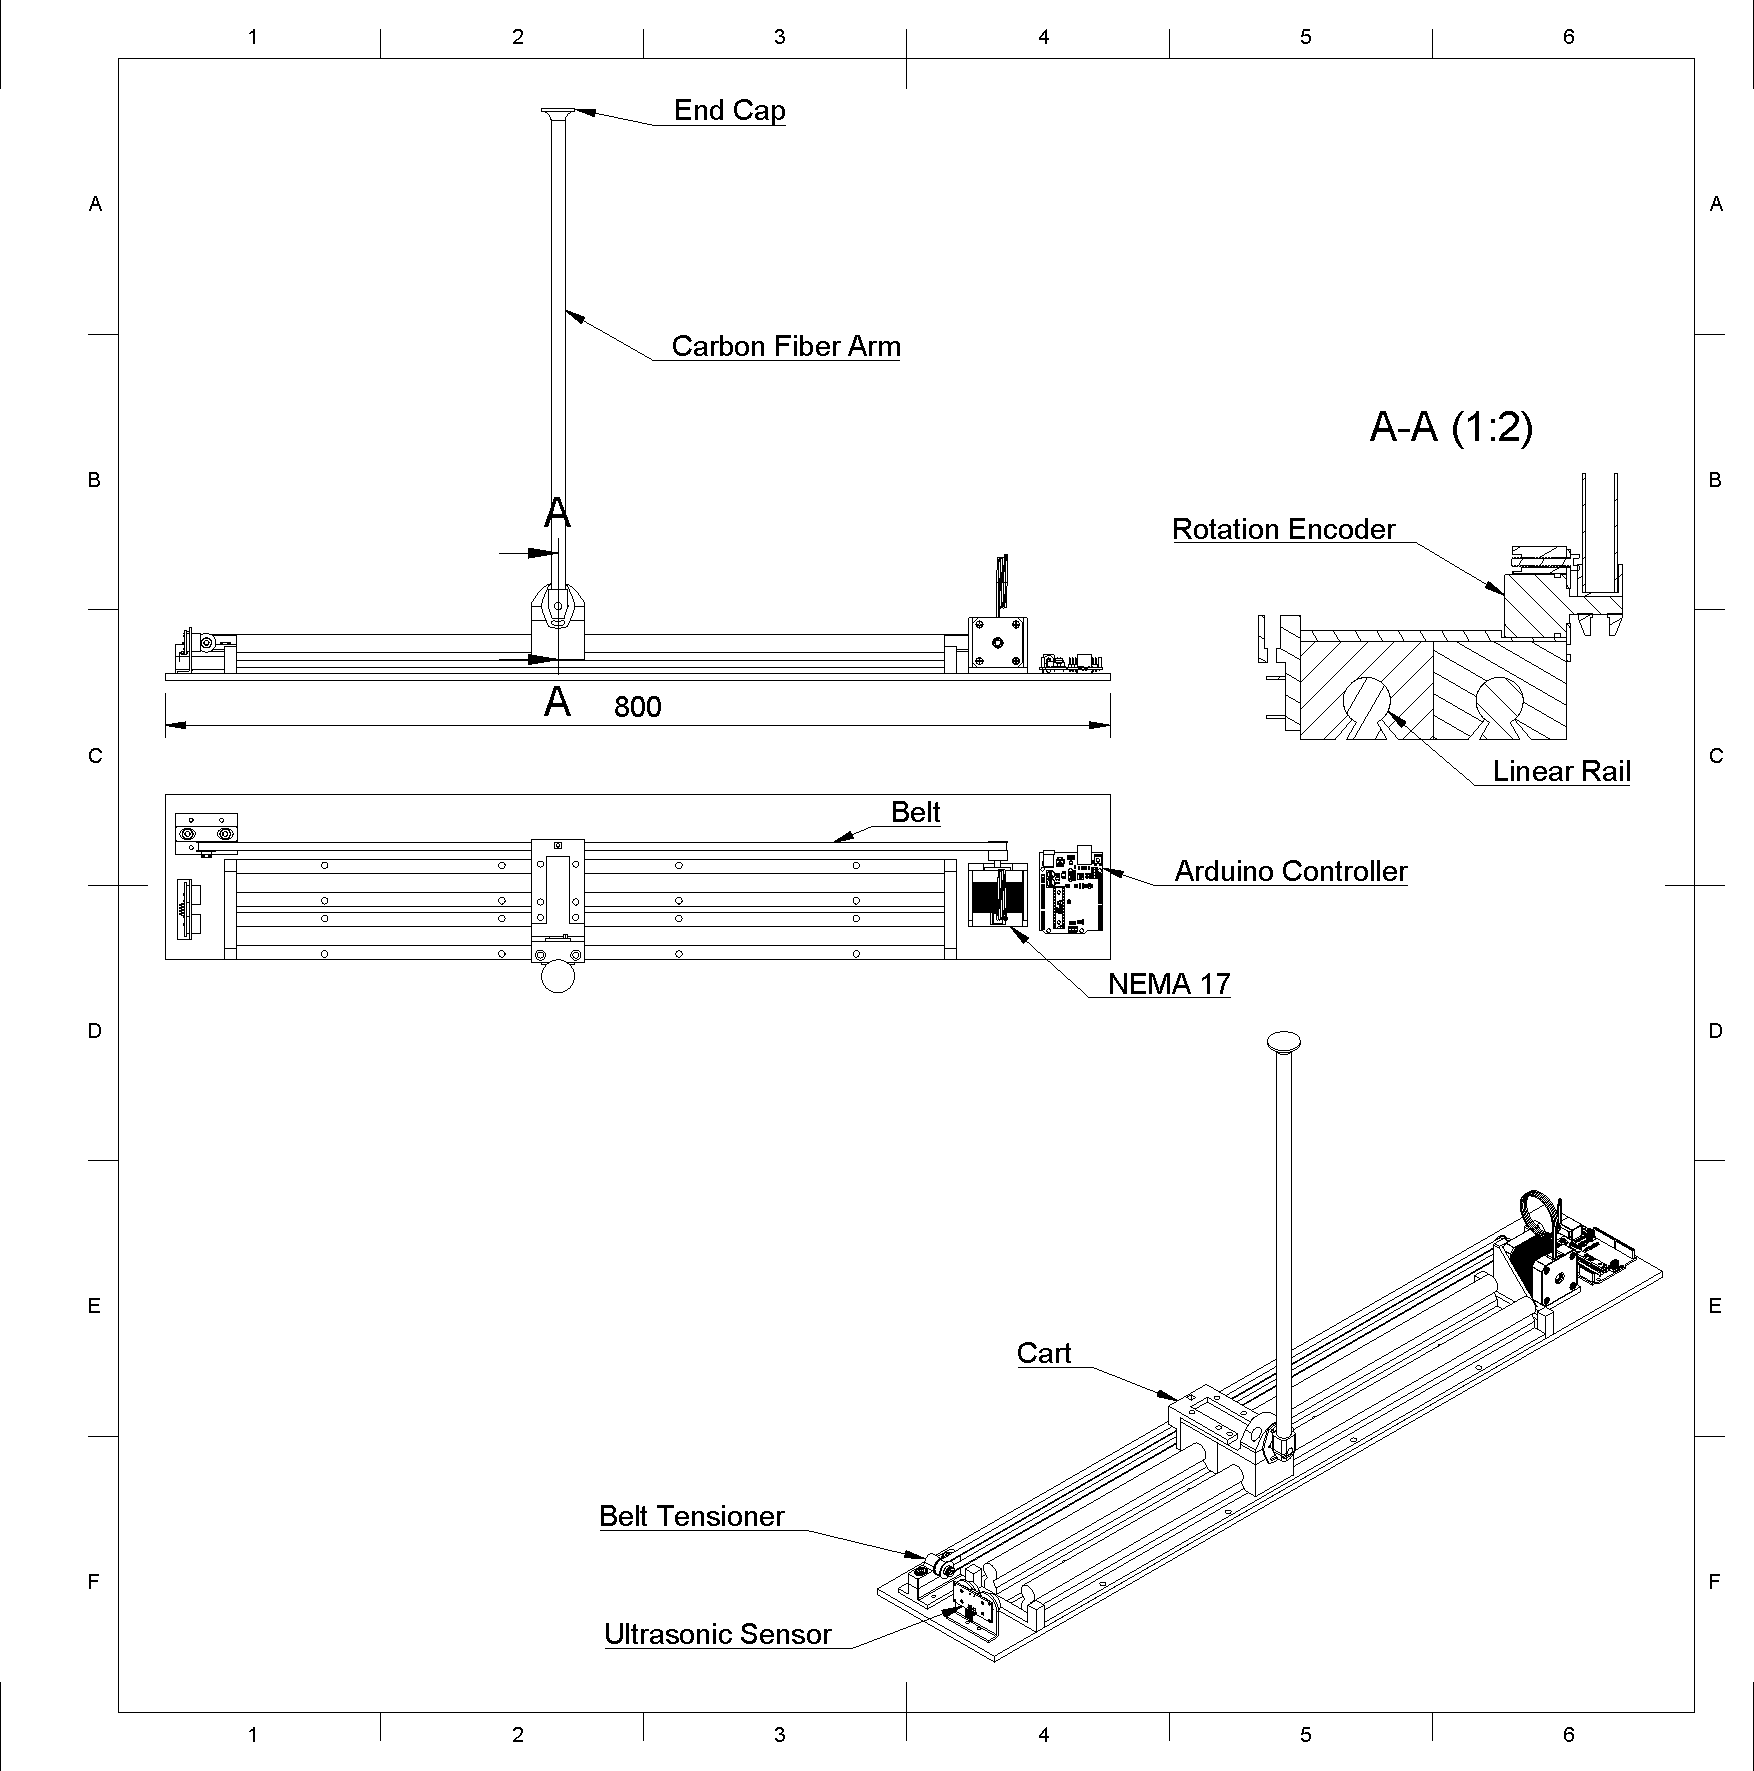
\includegraphics[width=\linewidth]{Images/InvertedPendulumSchematic.pdf}
    \caption{Inverted Pendulum Schematic}
    \label{fig:pend schem}
\end{figure}
A breakdown of the components in the pendulum is done below, considering both the electronics and mechanical systems which will inform the control system design.

\subsubsection{Mechanical Considerations}
The mechanics of the inverted pendulum and cart are fairly simple. The main consideration is the selection of the length of the rails, and ensuring that the friction and mass of the cart are as low as possible. In this design, rails of the SBR16 specification were selected, although many other types of rail systems may be used. Some other types of linear rails and bearings may permit a lower mass cart, which is desirable.

Another important criteria is the selection of the belt drive and pulley system, which will dictate the conversion between RPM and linear speed for the system. A larger diameter pulley will result in higher linear speeds for a given RPM, but will also require more torque. The belt drive system here uses a GT2 belt with 20 tooth pulleys. Other pulley diameters may be used if more precise control or higher speed output is desirable for the given application.

\subsubsection{Rotary Encoder}
In cross section A-A, the rotary encoder can be seen. The rotary encoder is one of the most important components in the design as the angle measurement of the arm is very important in understanding the dynamics of the system. The particular model used here can be found at \cite{noauthor_yuecoom_nodate}.

This rotary encoder is a hall effect sensor, so it is contactless. The sensor has 12-bit precision and can measure angles to a precision of $0.088\degree$ as a result. This type of sensor has much less sensor noise than a common potentiometer and also produces less resistance to rotation. This reduction in drag helps the pendulum arm rotate more freely. For this project, I have mounted the pendulum arm directly onto the end of the sensor. However, for heavier loads, it may be wise to place the load on a bearing instead of the sensor itself.

Another important feature of the rotary encoder is the sensor linearity. For this model, the sensor linearity is 0.3\% of the full scale, which means that the maximum deviation from the true output is less than 0.3\% of $360\degree$, or less than $1.08\degree$.

\subsubsection{Arm}
The design of the physical arm is also quite important to the development of a control model for the pendulum. For a pendulum undergoing small oscillations, the period is given by 
$$T=2\pi\sqrt{\frac{l}{g}}$$
From this relation, we can see that increasing the length will increase the period and make the system easier to control. Of course, this is quite different for the inverted case since the fixed point is unstable. However, this still gives a heuristic for how long the pendulum will take to fall.

If we want to be more precise, we may take the linear equations of motion in \eqautoref{eq:linear pend} and assume that the acceleration $\ddot{x}$ is 0:
$$I\ddot{\theta}=mgl\theta$$
The exact moment of inertia of the system may change, but the moment of inertia must always have units of $ml^2$. If we let $I=Cml^2$, then:
$$\ddot{\theta}=\frac{g}{Cl}\theta$$
We can see that for small angles, the acceleration of the pendulum away from the equilibrium position is inversely related to the length of the pendulum and the moment of inertia, $C$. For this reason, it is quite easy to balance a broom vertically, but balancing a pencil is almost impossible!

For our system then, we should choose values that make controlling the system possible without extraordinarily fast electronics or microcontrollers. At the same time, the arm should be easily carried around and not so large as to require a huge motor to move it. A length of around $0.5\ \mathrm{m}$ is a good compromise between the two. Assuming the arm has a moment of inertia that is the same as a thin rod, $\frac{1}{3}ml^2$, then the acceleration is around $6.3 \ \mathrm{rad/s^2}$ for an angle of  $5\degree$. After this point, nonlinear effects become quite prevalent and the analysis breaks down. Of course, smaller angles will exhibit rotational accelerations which are smaller in direct linear relation with the angle.

For further investigation, we can consider the linear acceleration that would be required to restore $\ddot{\theta}$ to 0 as a first approximation of the required linear acceleration required of the system. This can be done using \eqautoref{eq:theta double dot pend} and plugging in $\ddot{\theta}$ as $6.3 \ \mathrm{rad/s}$ and $\theta$ as $5\degree$:
$$\ddot{x}=l\ddot\theta-g\theta\approx1.72 \ \mathrm{m/s^2}$$
We can think of these conditions as a worst possible case, where the cart needs to accelerate rapidly to compensate for a large angular error. Ideally, the control system will maintain an angle less that $5\degree$. In this case, the system needs to have the capability of acceleration up to $1.72 \ \mathrm{m/s^2}$.

While this analysis is non-perfect, it is at least a good heuristic for selecting an appropriate arm length for the pendulum. For further analysis of non-linear dynamics, simulation is often a good idea. Computing the non-linear dynamics using MATLAB/Simulink and providing the control algorithm can give a good idea of the amount of acceleration, peak velocity, and torque the system will need. All of these will be crucial to the selection of motor for the project. The set up of such a simulation has been described in \autoref{sec:sim}.
\subsection{Noise and Data Dropouts}
Noisy data is quite common in real world sensors, especially those found in low cost electronics. This is especially prevalent when the derivative of a signal must be computed. One repercussion of computing the derivative of a signal is that high frequency components of the signal (where most of the noise resides) are amplified.\endnote{This can be seen by considering a signal that is decomposed into its Fourier series:
$$f(t)=\sum_{k=-\infty}^{\infty}a_ke^{ik\omega_0t}$$
Taking the time derivative of the signal yields:
$$\frac{df(t)}{dt}=i\omega_0\sum_{k=-\infty}^{\infty}ka_ke^{ik\omega_0t}$$
Application of Parseval's formula gives that:
$$\frac{1}{\tau}\int_0^\tau\left|\frac{df(t)}{dt}\right|^2dt={\omega_0}^2\sum_{k=-\infty}^{\infty}|ka_k|^2$$
Which makes it evident that the power in the higher frequencies of the signal has been amplified as compared to the original signal} 

Another problem that occurs with real world signals is data dropouts. Dropouts can be quite common for some sensors, such as the encoders of DC motors. One way to deal with data dropouts is to include some logic that checks the difference in the signal output. If the difference is greater than some expected threshold, the data is disregarded. An example of such a code for implementation into MATLAB or Simulink is shown below:
\begin{lstlisting}[style=Matlab-editor]
function filtered = filterEncoder(currVal)

persistent prevVal

% Initialize on first call
if isempty(prevVal)
    prevVal = currVal;
end

% Dropout detection
threshold = 200;  % Adjust based on your system

if abs(currVal - prevVal) > threshold
    % Bad reading: keep previous good value
    filtered = prevVal;
else
    % Good reading: update and pass through
    filtered = currVal;
    prevVal = currVal;
end
\end{lstlisting}

A "persistent" variable is one which maintains its value across multiple function calls. Depending on the type of dropouts, more advanced approaches may need to be taken.

Dealing with noise is often done through the application of a low-pass filter or a moving average filter. These filters induce some delay in the signal, but signal delay is often preferable to noisy data. Either of these filters can be added in Simulink.

\newpage
\printendnotes
\part{Advanced Topics in Controls and Physics}\label{part: advanced topics}
\begin{chapquote}{Claude Shannon}
    ``Mathematics is the tool specially suited for dealing with abstract concepts of any kind and there is no limit to its power in this field.''
\end{chapquote}

\newpage

\chapter*{Outline}

\color{red} This section is to be finished after the initial release of this volume. My apologies to any readers with particular interest in the methods of geometric control and differential geometry.\color{black}

In this final portion of the book, I will describe the methods of controls which are much beyond the standard coursework of a typical curriculum in engineering. This section will hold the information related to differential geometry, Lie theory, and it's application in the fields of geometric control (as well as some brief mention of the applications in physics). Such an understanding will require us to develop quite a bit of mathematics. The first several chapters will lay this mathematical foundation upon which our theories will be built.

This section is intended to live outside the scope of the rest of the book, such that the reader may stop their reading at the end of \autoref{part:control theory} and have gained all the necessary knowledge for a working understanding of control theory and energy mechanics. However, for those who want to dive deeply into these subject matter, this part will build off the rest of the book and dive into the study of advanced control theory and techniques. 

I start with a study of \gls{lie theory}, which will form a foundational knowledge of group theory and introduce us to the concepts of differentiable manifolds. From our study of \gls{lie theory}, the study of differentiable manifolds naturally arises. So, I devote this first section to a brief overview of Lie theory, differential geometry, and some applications. In fields such as geometric control, differential geometry plays a crucial part. The study of differential geometry should provide a satisfying unification of the ideas of Clifford algebras, \gls{lie theory}, and inner product spaces. It is truly one of the most profound mathematical generalizations of the ideas found in physics and engineering.

To supplement the information in this chapter, I have found that \cite{hirvonen_profound_nodate} has some quite readable and good articles on many of these topics. There are, of course, many other sources which are good for deep dives into any of these concepts.


\chapter{Lie Theory}\label{chap:lie theory}


\begin{chapquote}{Anthony Zee}
    ``It is almost as if the Creator of the universe understood Lie groups and decided to use them (a few of the simplest exemplars anyway) to construct the interactions among the fundamental particles that fill the universe. You
might call Him or Her an applied group theorist.''
\end{chapquote}
% \begin{chapquote}{Albert Camus}
%     ``If thought discovered in the shimmering mirrors of phenomena eternal relations capable of summing them up and summing themselves up in a single principle, then would be seen an intellectual joy of which the myth of the blessed would be but a ridiculous imitation.''
% \end{chapquote}

% clean up the notation for groups and ensure its all the same.

The goal until now has been to introduce the methods of \gls{Lagrangian} and \gls{Hamiltonian} mechanics and control theory in a way that does not require very rigorous mathematical formalisms. However, to tie up some of the loose ends, it is useful to introduce some mathematical concepts which can be used to understand these concepts on a more fundamental level. Along the way, we will also gain insight into the nature of rotations and curved spaces. Introducing these concepts will allow us to formalize huge swaths of the content covered in both Volume II and Volume III up to now, and will prove beneficial in the future endeavors of this volume as well.

This mathematical description is not strictly necessary to use the concepts mentioned throughout this book, but it is helpful for readers who hope to gain a full understanding of the content. I will warn that these chapters are likely the most technical in the book and will require significant effort from the reader. Throughout the chapter, I will slowly introduce the standard mathematical notation of proofs to use as a shorthand instead of writing everything out. This will help acquaint the reader if they are to read further on the subject matter discussed.

Since this is a heavy subject, supplemental resources will be useful. I have compiled a list of useful videos and texts to help explain \gls{lie theory}. Both of these video sources have good visuals that introduce \gls{lie theory} fairly intuitively. \cite{michael_penn_maths_2021} is more mathematically rigorous, but \cite{mathemaniac_what_2023} may be a better overall introduction. \gls{lie theory} is also used extensively in physics, so much material may be found in this domain. Two of my favorite sources in this domain are \cite{eigenchris_spinors_nodate} and \cite{zee_group_2016}.

For those readers who would like to dive deeper into the  subject or prefer written material to videos, I have included several good sources. Likely the best texts to read after this one is \cite{stillwell_naive_2008} and \cite{hall_lie_2015}, which both cover much of the basics of \gls{lie theory}.

\section{Motivation and Background}\label{sec:motivation and background lie}

Before we dive into the mathematical foundations of \gls{lie theory}, we should first examine why it is of importance to us. \gls{lie theory} is concerned with the inherit symmetries of mathematical objects. More specifically, the theory is concerned with so-called \textit{continuous symmetries}.

A big question is why do \textit{we} care? Well, it turns out that all of the rotations that we study are understood with \gls{lie theory}. It is also used to describe quaternions, symplectic groups (in Lagrangian and Hamiltonian mechanics), advanced control methods, robotics, and inertial navigation, just to name a few use cases. Gaining an intuition for the underlying mathematics will prove useful for us. 

For us, \gls{lie theory} is especially useful in our study of dynamic systems. Often, we do have symmetries in our problems. There are those symmetries that are obvious -- such as axial symmetry and reflectional symmetry of an object. There are deeper, more fundamental symmetries though, such as the symmetry between the rotational invariance of the Lagrangian and conservation of angular momentum (we will explore this more in \autoref{Noether's Theorem}).

Understanding symmetries is what led Sophus Lie to originally develop his theory. The study of discrete symmetries by Galois had proven very useful in understanding polynomial equations. Originally, Sophus Lie (shown in \autoref{fig:Lie}) developed the theory in order to understand the continuous symmetries of differential equations. However, the theory also proved to be useful in describing other symmetries, such as the rotations and conservation equations which we are familiar with in dynamics.

\begin{figure}[ht]
    \centering
    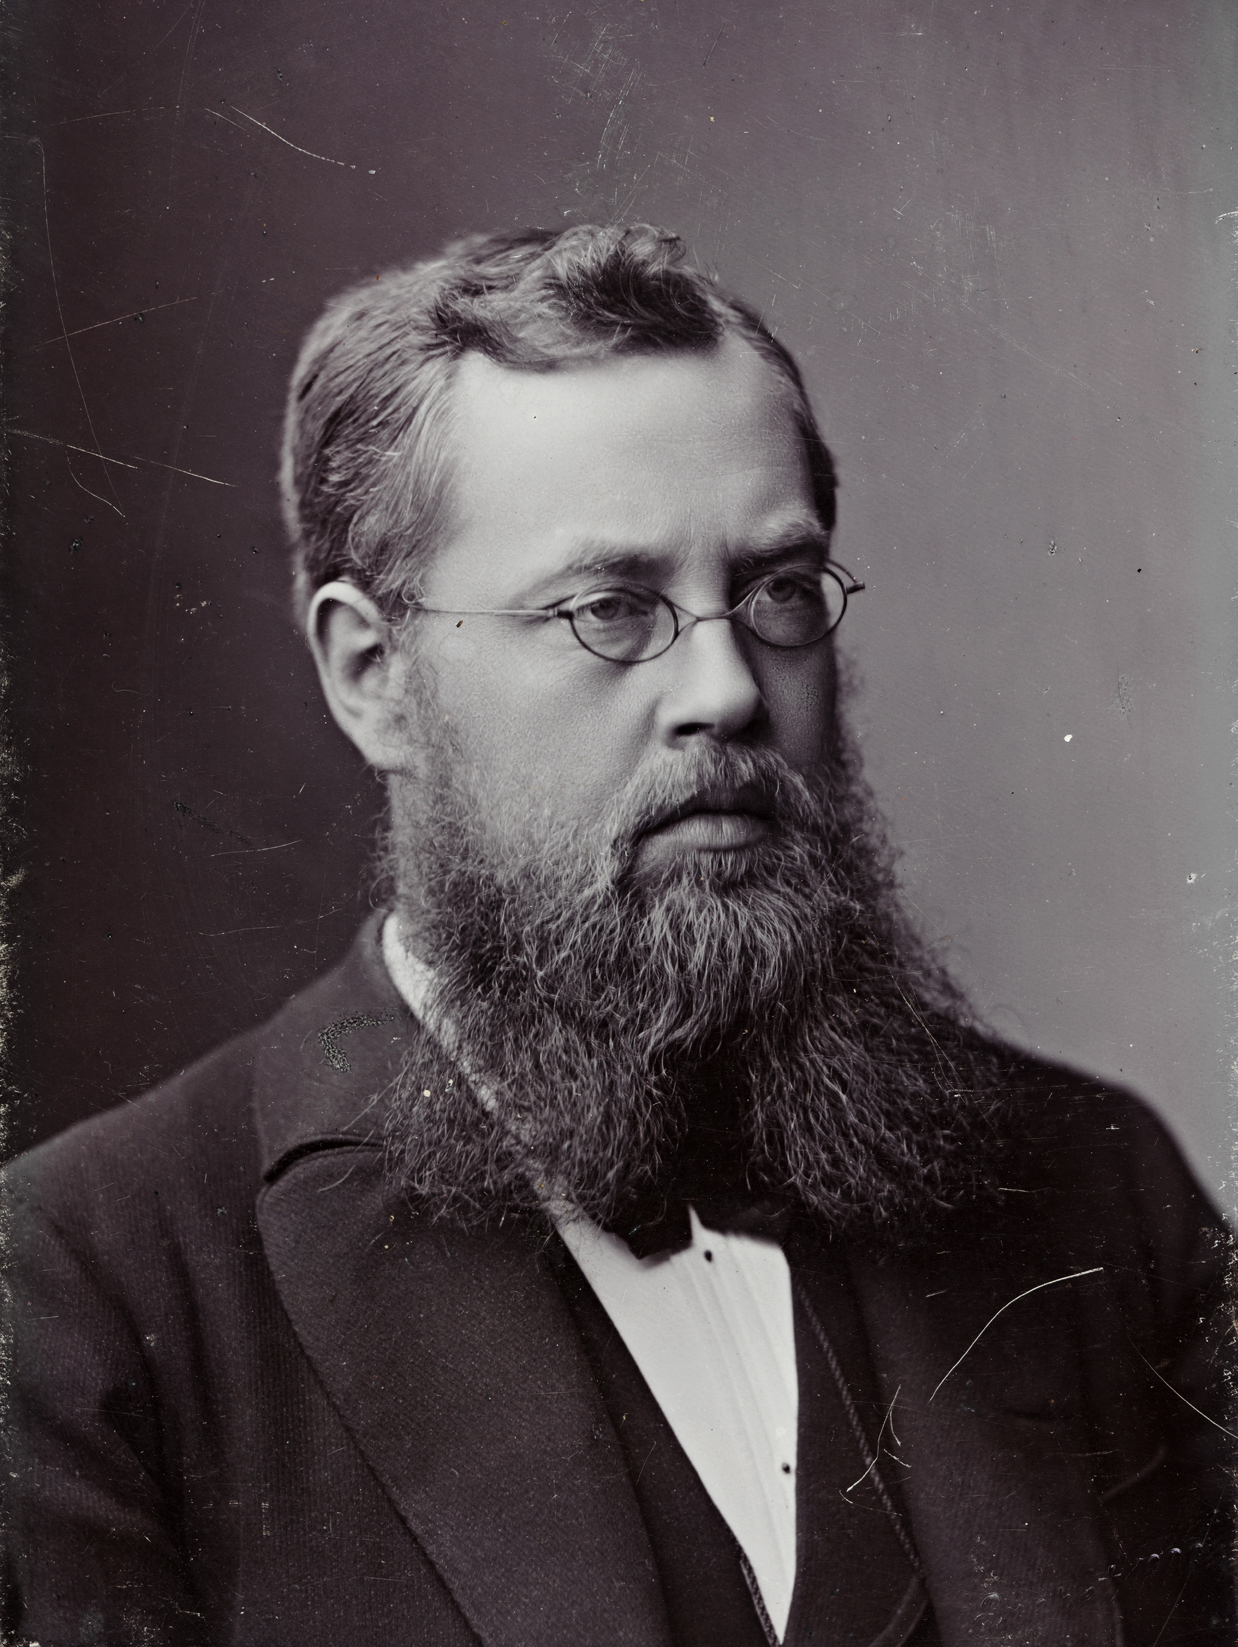
\includegraphics[width=0.5\linewidth]{Images/Portrett_av_Sophus_Lie.jpg}
    \caption{A Portrait of Sophus Lie}
    \label{fig:Lie}
\end{figure}

The big question, then, is how we can describe symmetry mathematically. A mathematical object known as a \textit{group} is the answer. Groups contain inherit information about symmetry. Lie theory extends this concept via the inclusion of \textit{manifolds} - which will be detailed later. The important conceptual understanding is that groups provide the symmetry, and the manifolds give a `language' to describe our system using a set of coordinates - much like we can describe any point on the surface of earth using latitude and longitude.\endnote{Some mathematicians will be quick to point out that manifolds don't necessarily need coordinates for their description. For calculations, however, we like to ascribe these qualities. In physics, it is typical that we use cartesian coordinates when we do this conversion to physical units, since they require no Jacobian.}

The other big part of \gls{lie theory} is that we can describe the attributes of our system at a point using \textit{algebras}. By thinking about our system as a manifold, we are able to describe coordinates for a certain location. Then, we can do something akin to a derivative - looking at the space `tangent' to the manifold at that point. This `tangent space' is what we call the \gls{lie algebra}.

\glspl{lie algebra} are useful because the tangent space is flat. Because it is flat, typical rules of geometry and calculus can be used, making analysis much easier. These algebras are essentially our computational tool that allows us to do simple calculations that yield complex results.

The last important thing to mention is that we can convert between the \gls{lie group} and the \gls{lie algebra} using something called an \gls{exponential map}. For some groups and operations, this \gls{exponential map} is simply an exponential function. Other times, however, we need a different way to describe these exponential transformations. This will be discussed later.

The most important thing to realize is that we can relate a complex non-linear system (represented in \gls{lie theory} by a group on a manifold) locally with a linearized version of the system, which we essentially `project' onto the system via the \gls{exponential map}. 

We've just gone through the premise of \gls{lie theory} at a blistering speed. We will dive into each aspect in much greater detail in the following chapters. What is important now is to understand the big picture ideas as we construct our mathematical ideas.

As a final point before we start, I believe that Lie theory is simply a beautiful theory which ties together so much mathematics. A careful study of Lie theory will unite many of the mathematical concepts you encounter.

\section{Groups and Symmetries}
\begin{chapquote}{Mark A. Armstrong}
    ``Numbers measure size, groups measure symmetry''
\end{chapquote}

Groups are extremely fundamental in the construction of Lie theory. As we have mentioned, groups provide the language of symmetries. They are conceptually simple but exceedingly powerful.\endnote{In fact, we see groups used very often in quantum mechanics and field theories. Groups are foundational in our understanding of why forces themselves exist!}

Before we get to formal definitions, it is helpful to have a mental picture of what a group is. From there, we can narrow our view to the concept of a  \gls{lie group}. 2-D Shapes are a good motivating example for what groups are at the basic level. We can consider a basic shape, like the equilateral triangle, as an example. What we define as the \textit{group} is the collection of symmetries that the triangle exhibits.

\begin{example}[The Symmetries of a Triangle]
A triangle is a good showcase of the symmetries that we find naturally in geometry. Let us consider an equilateral triangle as shown in \autoref{fig:eq triangle}.

\begin{figure}[H]
    \centering

\tikzset{every picture/.style={line width=0.75pt}} %set default line width to 0.75pt        

\begin{tikzpicture}[x=0.75pt,y=0.75pt,yscale=-1,xscale=1]
%uncomment if require: \path (0,300); %set diagram left start at 0, and has height of 300

%Shape: Triangle [id:dp8868857688850825] 
\draw  [color={rgb, 255:red, 74; green, 144; blue, 226 }  ,draw opacity=1 ][line width=2.25]  (330,70.47) -- (410,210) -- (250,210) -- cycle ;

% Text Node
\draw (236,212.4) node [anchor=north west][inner sep=0.75pt]    {$1$};
% Text Node
\draw (415,212.4) node [anchor=north west][inner sep=0.75pt]    {$2$};
% Text Node
\draw (325,48.4) node [anchor=north west][inner sep=0.75pt]    {$3$};

\end{tikzpicture}

    \caption{An Equilateral Triangle}
    \label{fig:eq triangle}
\end{figure}

It is natural to say that this triangle is symmetric, but what do we really mean when we say that? Mathematically, we're saying that we can perform some operation, which we may call $g$, and the result is that the triangle looks exactly identical afterward. 

The vertices of this triangle have only been labeled so that we can keep track of them as we perform actions on this triangle. If we don't have these labels, we couldn't see anything changing. This highlights one important thing about groups -- our group operations are those operations where we look at our object and we observe no measurable change.

Let's understand each symmetry of the triangle one at a time. We'll start with reflectional symmetries, like putting the triangle in a mirror. We can reflect about the vertical line through `3' as an example of such a symmetry.
\begin{figure}[H]
    \centering
    

\tikzset{every picture/.style={line width=0.75pt}} %set default line width to 0.75pt        

\begin{tikzpicture}[x=0.75pt,y=0.75pt,yscale=-1,xscale=1]
%uncomment if require: \path (0,300); %set diagram left start at 0, and has height of 300

%Shape: Triangle [id:dp8868857688850825] 
\draw  [color={rgb, 255:red, 74; green, 144; blue, 226 }  ,draw opacity=1 ][line width=2.25]  (330,70.47) -- (410,210) -- (250,210) -- cycle ;
%Straight Lines [id:da17313732782624203] 
\draw  [dash pattern={on 4.5pt off 4.5pt}]  (330,70.47) -- (330,210) ;

% Text Node
\draw (236,212.4) node [anchor=north west][inner sep=0.75pt]    {$2$};
% Text Node
\draw (415,212.4) node [anchor=north west][inner sep=0.75pt]    {$1$};
% Text Node
\draw (325,48.4) node [anchor=north west][inner sep=0.75pt]    {$3$};


\end{tikzpicture}
    \caption{Reflectional Symmetry of Triangle}
    \label{fig:triangle reflect}
\end{figure}
We can see that this action flips the locations of `1' and `2', but if we had not designated these points, we'd have no way of knowing the triangle was changed! For this reason, we call this action a symmetry of the triangle.

We can also rotate the triangle by $120
\degree$ about it's geometric center to get another indistinguishable triangle.
\begin{figure}[H]
    \centering

\tikzset{every picture/.style={line width=0.75pt}} %set default line width to 0.75pt        

\begin{tikzpicture}[x=0.75pt,y=0.75pt,yscale=-1,xscale=1]
%uncomment if require: \path (0,300); %set diagram left start at 0, and has height of 300

%Shape: Triangle [id:dp021503950787327253] 
\draw  [color={rgb, 255:red, 74; green, 144; blue, 226 }  ,draw opacity=1 ][line width=2.25]  (330,70.47) -- (410,210) -- (250,210) -- cycle ;
%Shape: Arc [id:dp6942684746026092] 
\draw  [draw opacity=0] (331.64,69.49) .. controls (382.91,70.36) and (424.2,112.19) .. (424.2,163.67) .. controls (424.2,180.24) and (419.92,195.82) .. (412.4,209.35) -- (330,163.67) -- cycle ; \draw    (334.71,69.59) .. controls (384.54,72.04) and (424.2,113.22) .. (424.2,163.67) .. controls (424.2,180.24) and (419.92,195.82) .. (412.4,209.35) ;  \draw [shift={(331.64,69.49)}, rotate = 4.65] [fill={rgb, 255:red, 0; green, 0; blue, 0 }  ][line width=0.08]  [draw opacity=0] (8.93,-4.29) -- (0,0) -- (8.93,4.29) -- cycle    ;

% Text Node
\draw (236,212.4) node [anchor=north west][inner sep=0.75pt]    {$2$};
% Text Node
\draw (415,212.4) node [anchor=north west][inner sep=0.75pt]    {$3$};
% Text Node
\draw (325,48.4) node [anchor=north west][inner sep=0.75pt]    {$1$};
% Text Node
\draw (377,116.4) node [anchor=north west][inner sep=0.75pt]    {$120\degree $};


\end{tikzpicture}

    \caption{Rotational Symmetry of a Triangle}
    \label{fig:rot triangle}
\end{figure}
In total, there are 6 ways that we can create a triangle which looks exactly the same as the one we started with. All of these are shown in \autoref{fig:sym tri}.
\begin{figure}[H]
    \centering
    

\tikzset{every picture/.style={line width=0.75pt}} %set default line width to 0.75pt        

\begin{tikzpicture}[x=0.75pt,y=0.75pt,yscale=-1,xscale=1]
%uncomment if require: \path (0,300); %set diagram left start at 0, and has height of 300

%Shape: Triangle [id:dp021503950787327253] 
\draw  [color={rgb, 255:red, 74; green, 144; blue, 226 }  ,draw opacity=1 ][line width=2.25]  (330,70.47) -- (410,210) -- (250,210) -- cycle ;
%Shape: Arc [id:dp6942684746026092] 
\draw  [draw opacity=0] (331.64,69.49) .. controls (382.91,70.36) and (424.2,112.19) .. (424.2,163.67) .. controls (424.2,180.24) and (419.92,195.82) .. (412.4,209.35) -- (330,163.67) -- cycle ; \draw    (334.71,69.59) .. controls (384.54,72.04) and (424.2,113.22) .. (424.2,163.67) .. controls (424.2,180.24) and (419.92,195.82) .. (412.4,209.35) ;  \draw [shift={(331.64,69.49)}, rotate = 4.65] [fill={rgb, 255:red, 0; green, 0; blue, 0 }  ][line width=0.08]  [draw opacity=0] (8.93,-4.29) -- (0,0) -- (8.93,4.29) -- cycle    ;
%Shape: Arc [id:dp18064647912182097] 
\draw  [draw opacity=0] (410.74,212.18) .. controls (384.35,256.14) and (327.48,270.98) .. (282.9,245.25) .. controls (268.55,236.96) and (257.2,225.47) .. (249.24,212.19) -- (330,163.67) -- cycle ; \draw    (409.12,214.79) .. controls (382.08,256.72) and (326.59,270.47) .. (282.9,245.25) .. controls (268.55,236.96) and (257.2,225.47) .. (249.24,212.19) ;  \draw [shift={(410.74,212.18)}, rotate = 124.65] [fill={rgb, 255:red, 0; green, 0; blue, 0 }  ][line width=0.08]  [draw opacity=0] (8.93,-4.29) -- (0,0) -- (8.93,4.29) -- cycle    ;
%Shape: Arc [id:dp048284149806032906] 
\draw  [draw opacity=0] (247.61,209.34) .. controls (222.74,164.5) and (238.32,107.83) .. (282.9,82.09) .. controls (297.25,73.81) and (312.88,69.73) .. (328.36,69.47) -- (330,163.67) -- cycle ; \draw    (246.17,206.63) .. controls (223.37,162.25) and (239.21,107.31) .. (282.9,82.09) .. controls (297.25,73.81) and (312.88,69.73) .. (328.36,69.47) ;  \draw [shift={(247.61,209.34)}, rotate = 244.65] [fill={rgb, 255:red, 0; green, 0; blue, 0 }  ][line width=0.08]  [draw opacity=0] (8.93,-4.29) -- (0,0) -- (8.93,4.29) -- cycle    ;
%Straight Lines [id:da4638366372358793] 
\draw  [dash pattern={on 4.5pt off 4.5pt}]  (330,70.47) -- (330,210) ;
%Straight Lines [id:da9032255747155441] 
\draw  [dash pattern={on 4.5pt off 4.5pt}]  (290,140) -- (410,210) ;
%Straight Lines [id:da6037792210940448] 
\draw  [dash pattern={on 4.5pt off 4.5pt}]  (370,140) -- (250,210) ;

% Text Node
\draw (236,212.4) node [anchor=north west][inner sep=0.75pt]    {$1$};
% Text Node
\draw (415,212.4) node [anchor=north west][inner sep=0.75pt]    {$2$};
% Text Node
\draw (325,48.4) node [anchor=north west][inner sep=0.75pt]    {$3$};
% Text Node
\draw (284,130) node [anchor=east] [inner sep=0.75pt]    {$240\degree $};
% Text Node
\draw (330,221.4) node [anchor=north] [inner sep=0.75pt]    {$360\degree $};
% Text Node
\draw (381,130) node [anchor=west] [inner sep=0.75pt]    {$120\degree $};

\end{tikzpicture}

    \caption{Symmetries of the Trangle}
    \label{fig:sym tri}
\end{figure}
    The very special thing about these symmetries is that we can do two (or more) of them -- one after the other -- and we get another symmetry of the group. Go ahead and try it! You'll find that no matter which operations you do, there's always a way to accomplish it with a single operation! This very special property is called \textit{closure}.
    There is one other thing, too

    One last thing to note: you'll notice that a rotation by $360\degree$ is equivalent to rotation by $0\degree$. This rotation effectively `does nothing'. This is what we call the identity element. Although it seems simple, it is a very important part of the group.

    This brief introduction should give you everything you need to help motivate the axiomatic treatment of groups and the \glspl{lie group} that are to follow.

    If you want more practice or explanation with these concepts, 3Blue1Brown has a good video to help introduce this concept, which has be found at \cite{3blue1brown_eulers_2017}.
\end{example}

What we have just seen with the triangle is an example of a \textit{discrete symmetry}; a symmetry which requires us to do a sort of `jump' to reach our next symmetry. Since the symmetry is discrete, we can count the total number of symmetries that we have. In the case of the triangle, we have our three rotations and three reflections, giving us a countable set of symmetries.

There is another type of symmetry that exists, and one that will in fact be far more useful for us. This type of symmetry is a \textit{continuous symmetry}. Sticking with our 2-D shapes, we can think about a circle instead:
\begin{figure}[ht]
    \centering

\tikzset{every picture/.style={line width=0.75pt}} %set default line width to 0.75pt        

\begin{tikzpicture}[x=0.75pt,y=0.75pt,yscale=-1,xscale=1]
%uncomment if require: \path (0,300); %set diagram left start at 0, and has height of 300

%Shape: Circle [id:dp012698292168043301] 
\draw  [color={rgb, 255:red, 74; green, 144; blue, 226 }  ,draw opacity=1 ][line width=2.25]  (250,135) .. controls (250,93.58) and (283.58,60) .. (325,60) .. controls (366.42,60) and (400,93.58) .. (400,135) .. controls (400,176.42) and (366.42,210) .. (325,210) .. controls (283.58,210) and (250,176.42) .. (250,135) -- cycle ;
%Shape: Arc [id:dp4686733674855805] 
\draw  [draw opacity=0] (408.95,92.23) .. controls (415.5,105.06) and (419.2,119.6) .. (419.2,135) .. controls (419.2,187.02) and (377.02,229.2) .. (325,229.2) .. controls (312.52,229.2) and (300.6,226.77) .. (289.7,222.36) -- (325,135) -- cycle ; \draw    (410.28,94.95) .. controls (416,107.1) and (419.2,120.68) .. (419.2,135) .. controls (419.2,187.02) and (377.02,229.2) .. (325,229.2) .. controls (312.52,229.2) and (300.6,226.77) .. (289.7,222.36) ;  \draw [shift={(408.95,92.23)}, rotate = 66.66] [fill={rgb, 255:red, 0; green, 0; blue, 0 }  ][line width=0.08]  [draw opacity=0] (8.93,-4.29) -- (0,0) -- (8.93,4.29) -- cycle    ;
%Straight Lines [id:da10366016362761077] 
\draw  [dash pattern={on 4.5pt off 4.5pt}]  (325,135) -- (289.7,222.36) ;
%Straight Lines [id:da8482728300676312] 
\draw  [dash pattern={on 4.5pt off 4.5pt}]  (325,135) -- (408.95,92.23) ;

% Text Node
\draw (271,222.4) node [anchor=north west][inner sep=0.75pt]    {$1$};
% Text Node
\draw (421,72.4) node [anchor=north west][inner sep=0.75pt]    {$2$};
% Text Node
\draw (401,202.4) node [anchor=north west][inner sep=0.75pt]  [font=\large]  {$\theta $};


\end{tikzpicture}


    \caption{Symmetries of a circle}
    \label{fig:circle sym}
\end{figure}

In contrast with the triangle, this circle may be rotated through \textit{any} angle or reflected about any axis. Mathematically, what makes this different is that it requires no `jump' to go from one symmetry to the next. Our symmetries are continuous as we go around the circle. In fact, the circle group, which we often denote $\mathbb{S}^1$, is one of the prototypical examples of a \gls{lie group}. This smoothly varying structure is in fact the definitive concept us to define this as a \gls{lie group}.
\footnote{If you want to dive deeper into group theory, a wonderful introductory text can be found in \cite{armstrong_groups_1988}.}

\section{Lie Groups}
The \gls{lie group} is in essence a group and a manifold, which is shown in \autoref{fig:Lie Group}:
\begin{figure}[ht]
    \centering





% Gradient Info
  
\tikzset {_5g6glwol0/.code = {\pgfsetadditionalshadetransform{ \pgftransformshift{\pgfpoint{93.6 bp } { -132.6 bp }  }  \pgftransformscale{1.04 }  }}}
\pgfdeclareradialshading{_kg48z90ds}{\pgfpoint{-96bp}{136bp}}{rgb(0bp)=(1,1,1);
rgb(0bp)=(1,1,1);
rgb(25bp)=(0.29,0.56,0.89);
rgb(400bp)=(0.29,0.56,0.89)}
\tikzset{_v4ek6umsw/.code = {\pgfsetadditionalshadetransform{\pgftransformshift{\pgfpoint{93.6 bp } { -132.6 bp }  }  \pgftransformscale{1.04 } }}}
\pgfdeclareradialshading{_66pto071l} { \pgfpoint{-96bp} {136bp}} {color(0bp)=(transparent!40);
color(0bp)=(transparent!40);
color(25bp)=(transparent!50);
color(400bp)=(transparent!50)} 
\pgfdeclarefading{_h77ttbdia}{\tikz \fill[shading=_66pto071l,_v4ek6umsw] (0,0) rectangle (50bp,50bp); } 
\tikzset{every picture/.style={line width=0.75pt}} %set default line width to 0.75pt        

\begin{tikzpicture}[x=0.75pt,y=0.75pt,yscale=-1,xscale=1]
%uncomment if require: \path (0,300); %set diagram left start at 0, and has height of 300

%Straight Lines [id:da6341386319589457] 
\draw    (292.14,174.29) -- (292.14,12) ;
\draw [shift={(292.14,10)}, rotate = 90] [color={rgb, 255:red, 0; green, 0; blue, 0 }  ][line width=0.75]    (7.65,-2.3) .. controls (4.86,-0.97) and (2.31,-0.21) .. (0,0) .. controls (2.31,0.21) and (4.86,0.98) .. (7.65,2.3)   ;
%Straight Lines [id:da24449585878217006] 
\draw    (292.14,174.29) -- (438,174.29) ;
\draw [shift={(440,174.29)}, rotate = 180] [color={rgb, 255:red, 0; green, 0; blue, 0 }  ][line width=0.75]    (7.65,-2.3) .. controls (4.86,-0.97) and (2.31,-0.21) .. (0,0) .. controls (2.31,0.21) and (4.86,0.98) .. (7.65,2.3)   ;
%Straight Lines [id:da20393695102666232] 
\draw    (292.14,174.29) -- (211.41,255.01) ;
\draw [shift={(210,256.43)}, rotate = 315] [color={rgb, 255:red, 0; green, 0; blue, 0 }  ][line width=0.75]    (7.65,-2.3) .. controls (4.86,-0.97) and (2.31,-0.21) .. (0,0) .. controls (2.31,0.21) and (4.86,0.98) .. (7.65,2.3)   ;

%Shape: Donut [id:dp3968285728219174] 
\draw  [draw opacity=0][shading=_kg48z90ds,_5g6glwol0,path fading= _h77ttbdia ,fading transform={xshift=2}] (283.14,135.41) .. controls (283.14,135.41) and (293.7,141.26) .. (306.72,148.48) .. controls (319.74,155.7) and (330.3,161.55) .. (330.3,161.55) .. controls (330.3,161.55) and (319.74,155.7) .. (306.72,148.48) .. controls (293.7,141.26) and (283.14,135.41) .. (283.14,135.41)(194.07,86.04) .. controls (223.35,37.96) and (297.53,26.94) .. (359.75,61.43) .. controls (421.97,95.92) and (448.66,162.85) .. (419.37,210.93) .. controls (390.09,259) and (315.91,270.02) .. (253.69,235.53) .. controls (191.47,201.04) and (164.78,134.11) .. (194.07,86.04) ;
%Straight Lines [id:da060154956904347356] 
\draw [color={rgb, 255:red, 218; green, 44; blue, 0 }  ,draw opacity=1 ]   (340.26,220) ;
\draw [shift={(340.26,220)}, rotate = 0] [color={rgb, 255:red, 218; green, 44; blue, 0 }  ,draw opacity=1 ][fill={rgb, 255:red, 218; green, 44; blue, 0 }  ,fill opacity=1 ][line width=0.75]      (0, 0) circle [x radius= 2.34, y radius= 2.34]   ;
%Straight Lines [id:da47247361109034747] 
\draw [color={rgb, 255:red, 218; green, 44; blue, 0 }  ,draw opacity=1 ]   (380.26,210) ;
\draw [shift={(380.26,210)}, rotate = 0] [color={rgb, 255:red, 218; green, 44; blue, 0 }  ,draw opacity=1 ][fill={rgb, 255:red, 218; green, 44; blue, 0 }  ,fill opacity=1 ][line width=0.75]      (0, 0) circle [x radius= 2.34, y radius= 2.34]   ;
%Straight Lines [id:da7815998594768269] 
\draw [color={rgb, 255:red, 218; green, 44; blue, 0 }  ,draw opacity=1 ]   (230.26,150) ;
\draw [shift={(230.26,150)}, rotate = 0] [color={rgb, 255:red, 218; green, 44; blue, 0 }  ,draw opacity=1 ][fill={rgb, 255:red, 218; green, 44; blue, 0 }  ,fill opacity=1 ][line width=0.75]      (0, 0) circle [x radius= 2.34, y radius= 2.34]   ;
%Straight Lines [id:da8835218032244371] 
\draw    (370,110) -- (420,90) ;

% Text Node
\draw (331.26,222.4) node [anchor=north west][inner sep=0.75pt]  [color={rgb, 255:red, 218; green, 44; blue, 0 }  ,opacity=1 ]  {$g_{1}$};
% Text Node
\draw (371.26,212.4) node [anchor=north west][inner sep=0.75pt]  [color={rgb, 255:red, 218; green, 44; blue, 0 }  ,opacity=1 ]  {$g_{2}$};
% Text Node
\draw (216.26,152.4) node [anchor=north west][inner sep=0.75pt]  [color={rgb, 255:red, 218; green, 44; blue, 0 }  ,opacity=1 ]  {$g_{1} g_{2}$};
% Text Node
\draw (296,11.4) node [anchor=north west][inner sep=0.75pt]    {$\mathbb{R}^{n}$};
% Text Node
\draw (347,22.4) node [anchor=north west][inner sep=0.75pt]    {$g_{1} ,g_{2} ,g_{1} g_{2} \in \mathbb{R}^{n}$};
% Text Node
\draw (423,79.4) node [anchor=north west][inner sep=0.75pt]    {$G$};


\end{tikzpicture}



    \caption{Visualization of the Lie Group}
    \label{fig:Lie Group}
\end{figure}
What exactly does it mean for the \gls{lie group} to be both a group and a manifold?

The blue `orb' denoted $G$ is representative of a smooth manifold in $\mathbb{R}^n$. We can think of the manifold in this example as the surface of a 2D ellipsoid on which all the members of the group must live. We can see three points defined $g_1$, $g_2$, and $g_1\cdot g_2$. In this example, $g_1\cdot g_2$ is simply the multiplication of $g_1$ and $g_2$. We can remember from our triangle example that the product $g_1\cdot g_2$ must also be in the group because of closure.

The property that must hold for a \gls{lie group} is that not only do all $g_1,g_2,g_1\cdot g_2$ reside in $\mathbb{R}^n$, but additionally also lie on the surface of the ellipsoid! In other words, $g_1,g_2,g_1\cdot g_2\in G$. Now that we have a mental picture, we can move on to the formal definition.

\subsection{The Axioms of Groups}
As mentioned before, the defining feature of the \gls{lie group} is that it is both a group and a manifold. We must first define the attributes of a group if we are to formally define this concept. 

A group is a mathematical \textit{set} which obeys the following four properties for a given \textit{binary operation}. These properties are shown formally and then explained afterward.

\begin{enumerate}
\item $Closure{:} \mathrm{\ for \ all\ } g,h \in G, g\cdot h \in G$
\item $Associativity{:} \mathrm{\ for \ all \ } g,h,k \in  G, (g\cdot h)\cdot k=g\cdot(h\cdot k)$
\item $Identity{:} \mathrm{\ there \ is  \ } e\in G, \mathrm{\ for \ all \ } g \in G, e\cdot g=g\cdot e=g$
\item $Inverse{:} \mathrm{\ for \ all \ } g \in G, \mathrm{\ there \ is  \ } h \in G, g \cdot h=h\cdot g =e$
\end{enumerate}


I will now go over all of these properties to explain their meaning in more natural language for readers not familiar with the notation above.

\begin{enumerate}
    \item By closure, we mean that when we apply an operation on a \textit{set}, we get another element of that set. This is best motivated by an example. 

    Let us take the natural numbers, denoted $\mathbb{N}$ to be our set. The natural numbers are given as $1,2,3\cdots$  and so on. We say that the natural numbers are closed under addition, because adding any of the elements of the set together, we get another element of the set. For example, adding $1$ and $3$, we get $4$, which is also in the set $\mathbb{N}$. Moreover, any composition of these operations will also be part of the set. Performing addition twice will still give an element of the sequence. 
    
    Connecting this to our notation, we say that two elements, $g$ and $h$ are in the set $G$, which we represent with this notation: $g,h \in G$. We define the operation to be `$\cdot$', which is the notation for a general operation. We can then say that the elements, when acted upon by this operation, are still in the set $G$: $g\cdot h \in G$. This is what the formal definition of closure is.
    \item Associativity is a more simple concept which most readers are likely familiar with. It simply means that the grouping of the operations does not matter. Note that associativity \textit{does not} imply communitivity! If we take the example of matrices, $(AB)C=A(BC)$, which is an expression of associativity, but $AB\neq BA$ for matrices. 
    \item Identity is also relatively simple. Identity simply means that there exists an element of the set $G$, which when applied on another element of set $G$, has no effect. For the real numbers, $\mathbb{R}$, multiplication by the number $1$ is an example of an identity element.
    \item Inverse is the last property, which states that for each element in the set, there is another element in the set, that when acted upon by an operation, returns the identity. This is analogous to the inverse of a number, or inverse of a function, which you have studied in algebra.
\end{enumerate}

Lastly, I will explain what a \textit{binary operation} is. Stated simply, a binary operation is an operation which takes in two inputs and returns a single output. Most operations, such as addition, subtraction, and multiplication are binary. Basically, a binary operation is a simple mathematical operation between two numbers that you are familiar with.

\subsubsection{Further Group Examples}

Let's solidify our understanding of groups with some examples. Some of these are worked examples (blue), and some will require the reader to work through them (red).

\begin{example}[The Real Numbers]
    To wrap our minds around the concepts of groups, we consider the example of the integers, $\mathbb{Z}$.

    To check if the integers form a group, we first need to define our operation. We will choose addition. Then, we simply check each of the properties. 
    
    We have shown previously that adding any two natural numbers gives another natural number, and we can intuitively extend this to the integers as well. Next, we consider the associativity. It is easily seen that $(a+b)+c=a+(b+c)$, since addition is associative. Next, we consider the identity. For the operation of addition, the identity is the number $0$, which when added to any integer, $z$, does nothing. Lastly, we consider the inverse. We should have for every integer another integer such that $a+b=0$. It is obvious that $b=-a$, which is satisfied since the integers include negative numbers. Thus, we have shown that the integers are closed under addition.
\end{example}

The axioms of groups can be applied to create a group from any set of objects. In our study, it is most helpful to assign group identities to matrices, since our studies of rotations and control systems involve matrices heavily.

\begin{exercise}
We have shown in the previous example how the real numbers are closed under addition. Using the same axiomatic approach,  show why the integers are not a group under multiplication. Which axiom(s) is/are violated?
\end{exercise}

\begin{exercise}
    We have shown that we can make groups out of the elements of the number line. Previously, we have stated that groups contain information about symmetries. Think about the symmetries that are associated with the number line. How are these different than the symmetries associated with geometry? 
    
    Symmetries, typically, are quite broad! Here are just a few examples that you can try. See if you can explain what symmetries may exist for these objects:
    \begin{itemize}
        \item Functions (even, odd)
        \item Matrices
        \item Taylor Series
    \end{itemize}
There are many more types of symmetries which you may encounter if you further study mathematics!
\end{exercise}



\begin{example}[The Quaternion Group]
We have shown in Volume II that the quaternions form an algebra which we call $\mathbb{H}$. We define the elements of $\mathbb{H}$:
$q=q_0+q_1i+q_2j+q_3k ,\quad q_0,q_1,q_2,q_3\in\mathbb{R}$
    More specifically, this algebra is a four-dimensional associate unital algebra. We have the four dimensions defined by the basis: $1,i,j,k$. These elements are associative, meaning that the order in which we perform operations does not matter (However, the operations are not commutative!). Unital simply means that the algebra contains an identity element.

    We can again show all of the properties of the \gls{lie group} hold for the quaternion algebra.

    \begin{enumerate}
        \item Closure: We can show the closure of the group by considering the multiplication of any element of the quaternion group with any other element.
$$\begin{array}{c|cccc}
     \times&1&i&j&k  \\
     \hline
     1&1&i&j&k\\
     i&i&-1&k&-j\\
     j&j&-k&-1&i\\
     k&k&j&-i&-1\\
\end{array}$$
As we can see, the there is no multiplication that we can do that gives an element outside of the group. Therefore, the quaternions are closed under multiplication.
\item Associativity: An exact proof of the associativity of quaternions follows from the Cayley-Dickson construction of the quaternions or from Clifford algebras (which are discussed in Volume II). This is not immediately evident, but it is true that the quaternions are associative. More information can be found in \cite{michael_penn_climbing_2023} for the approach using the Cayley-Dickson construction or in \cite{sudgylacmoe_swift_2020} for the approach using Clifford algebras.
\item Identity: The identity element of the quaternions is simple, it is the element which contains only a real part of 1 and no other element.
\item Inverse: The inverse for the quaternions is also fairly simple. We can see from the multiplication table that any element of the quaternion algebra multiplied by itself gives the negative of the identity. So, we can simply multiply one of these terms by $-1$ to construct the identity. Since $-1$ is in the span of the real numbers, this is perfectly fine to do!


    \end{enumerate}
    So we have shown that the quaternions form both an algebra and a group! This is a quite interesting property. See if there are any other common mathematical objects that you can find group representations for!
\end{example}

\begin{exercise}[The Octonion Group (Hard)]

The octonions are an example of another algebra. The octonions have 8 elements and are denoted by $\mathbb{O}$. The octonians are typically expressed as $x=x_0e_0+x_1e_1+x_2e_2+x_3e_3+x_4e_4+x_5e_5+x_6e_6+x_7e_7$. It is also possible to express an octonion as a pair of quaternions.

\begin{enumerate}
    \item Use the Cayley-Dickson construction to create the octonions. From the construction, what property of the quaternions have you lost?
    \item With this knowledge, do the octonians form a group?

\end{enumerate}
\end{exercise}

\subsection{Representation Theory}
It is useful that we can describe groups axiomatically, but it is hard to do mathematical operations with groups. Luckily, we can express most groups in a way that is simpler to perform mathematical operations on. This is part of a field of mathematics called \textit{Representation Theory}.

The key realization is that it is possible to represent almost any group using a matrix! In the lingo of math, we are looking for a matrix that is \textit{isomorphic} to our group. An isomorphism means that the structure and information is indistinguishable, even if we have changed how we represent our object. Using representation theory, we typically denote this representation as $\rho$. We can then write the representation:
$$\rho:G\rightarrow GL(V)$$
We would say that `$\rho$' is a representation which maps our group $G$ onto $GL(V)$. We haven't discussed $GL(V)$ yet -- but it is simply a matrix group. If interested, you may read more on \autoref{thm:cayley} and \autoref{thm:Ado} which are foundational in proving why this matrix representation holds.

\begin{theorem}[Cayley's Theorem]\label{thm:cayley}
    Every group $G$ is isomorphic to a subgroup of the symmetric group.
\end{theorem}
\begin{theorem}[Ado's Theorem]\label{thm:Ado}
    Every finite-dimensional \gls{lie algebra} over a field $K$ of characteristic zero can be viewed as a \gls{lie algebra} of square matrices under the commutator bracket.
\end{theorem}

Interested readers can look into  which describe the details behind why this is true. These theorems will not be used elsewhere in this text, they are simply shown for completeness. More important than the proof is the result, which directly implies that we only need to know the field, $V$, we are operating in and some properties of the matrices.

An important implication of this theorem is that we may also represent any \gls{lie algebra} using this same matrix method. Knowing that we can represent groups like this gives us a great amount of computational power. Because we are well versed in linear algebra, we may use our tools from there to gain a robust understanding of \gls{lie theory}. Because this matrix representation is so useful, the rest of this chapter will focus on how we may represent these groups and perform math with them using the matrix representation of the group.

\subsection{Matrix Multiplication Groups}\label{sec:matrix groups}
To define matrix groups under multiplication, we need to again satisfy all four criteria of groups. For matrices, there are some subtleties that are worth covering in depth.

There are a few types of matrix multiplication groups that are important for our purposes. As noted before, $GL(V)$ is an important group to cover. All other groups will come from $GL(V)$, so it is the most important to describe. Before we get started, let's discuss our matrix group notation. Our field is what is denoted by $V$. As mentioned before, this field is the space that we operate in. For example, we may have $GL(\mathbb{R})$, which we read as `the general linear group with the real numbers as our field'. Often, we forego the description of the field because we so often use the real numbers. In that case, we may write $GL(n)$, which means that we are operating with a matrix with size $n\times n$.

To get started, let's figure out how we can derive $GL(n)$ before moving on to some of our more advanced groups. First, we will only consider $n{\times} n$ square matrices so that we can apply matrix multiplication from either direction freely. We can then proceed to see what conditions are necessary for this to be a group, which we will call $GL$. We will denote the size, $n$, in parenthesis, giving us $GL(n)$ as our group for matrices of size $n{\times}n$. To write the group in full, we need to also specify the field that we are considering. 

Typically, there are 3 fields that we consider. Those being the real numbers $(\mathbb{R})$, complex numbers $(\mathbb{C})$, and quaternions $(\mathbb{H})$.\endnote{The quaternions do not actually form a field since their multiplication is not commutative. However, we still consider them as an option over which we can define our field because the algebra of quaternions, $\mathbb{H}$, is isomorphic to $\mathbb{R}$ $(\mathbb{H}\cong\mathbb{R})$, so we are fine to use it in our field.} For now, for the sake of simplicity, we will consider the real numbers, so we would write $GL(n,\mathbb{R)}$ or $GL_2(\mathbb{R})$. I prefer to use the shorthand of $GL(n)$ since it is understood we are only considering reals for now. Other sources may prefer one of the other two notations.

Let's remember our four group axioms, as those are what we will need to construct our matrix group:

\begin{enumerate}
\item $Closure{:} \mathrm{\ for \ all\ } g,h \in G, g\cdot h \in G$
\item $Associativity{:} \mathrm{\ for \ all \ } g,h,k \in  G, (g\cdot h)\cdot k=g\cdot(h\cdot k)$
\item $Identity{:} \mathrm{\ there \ is  \ } e\in G, \mathrm{\ for \ all \ } g \in G, e\cdot g=g\cdot e=g$
\item $Inverse{:} \mathrm{\ for \ all \ } g \in G, \mathrm{\ there \ is  \ } h \in G, g \cdot h=h\cdot g =e$
\end{enumerate}

Starting with closure, we can write the following for any two matrices $A,B\in\mathbb{R}$:
$$AB \in GL $$
Without additional information about $A$, $B$, and $GL$, it is hard to define additional properties at this point. We will come back to this after establishing some of the other identities.

The property of associativity also does not help much, since all $n{\times} n$ matrices must satisfy associativity by the nature of matrix multiplication:
$$(AB)C=A(BC)$$
The first information about this group comes from the identity property. There must exist some square $n{\times} n$ matrix such that multiplication of the identity on either side of $A$ returns $A$.

\begin{proof}
\textbf{Identity Matrix}\\
    We know from intuition that this identity matrix is of the form:
$$\mathbb{I}(n)=\begin{bmatrix}
    1 & 0  &\cdots &0\\
    0&1&\cdots&0\\
    \vdots&\vdots&\ddots&0\\
    0&0&0&1
\end{bmatrix}$$

This can be proved using the fact that matrix multiplication takes the form
$$(AB)_{ij}=\sum_{k=1}^n{A_{ik}}{B}_{kj}$$
and noticing that the identity matrix takes the form of Kronecker delta $\delta_{ij}$ such that $\delta_{ij}=1$ when $i=j$ and is zero otherwise.

In effect, if we take $A$ to be the identity matrix, we can see that the product will only exist when $i=k$ in the sum. As a result the sum is effectively reduced to a single term because $k$ can only attain one possible value, $i$:
$$(AB)_{ij}={A_{ii}}{B}_{ij}$$
We have also defined the Knonecker delta $\delta_{ij}$ such that $\delta_{ii}=1$. Thus $A_{ii}$ also has a value of 1. From here, we can see that the equality reduces to
$$(AB)_{ij}={B}_{ij}$$
So, when matrix $A$ is the identity, it has the property of an identity element. Remember that we need this `do nothing' identity element in every group. It is a basic property that all matrix multiplication groups have $\mathbb{I}$!

So, we have shown that the matrix $\mathbb{I}(n)$ must be the identity element of the group $G(n)$.
\end{proof}

The last property is an inverse property, such that for all elements in $GL(n)$, there must exist another matrix in $GL(n)$ that when multiplied by returns $\mathbb{I}(n)$. 

\begin{proof}
\textbf{Square Matrix Inverse}\\
In linear algebra, it is known that a square matrix has an inverse if and only if the determinant is non-zero. This is proven by the invertible matrix theorem.
\end{proof}
Because the determinant must be non-zero, the columns of any element of $GL(n)$ must be linearly independent from the invertible matrix theorem. This is an important result, as it puts a definitive constraint on which matrices are part of $GL(n)$. Only the matrices with $n$ linear independent columns will be elements of $GL(n)$.

As a last step, we can go back and check that $GL$ is closed under the conditions that we described. 
\begin{proof}
\textbf{Closure of $\mathbf{GL(n)}$}\\
Supposing that matrices $A,B \in GL(n)$, we know that both have positive determinants from the invertible matrix theorem. We can then use the fact that $\det(AB)=\det(A)\det(B)$. Since $\det(A)>0$ and $\det(B)>0$, it must be true that $\det(AB)>0$ and thus $AB \in GL(n)$.
\end{proof}

So, we have proven the most general group of $n{\times}n$ invertible matrices, which is called $GL(n)$ for the \textit{general linear group}.

\subsection{The role of the determinant}\label{sec:role of the determinant}

The determinant has a special meaning in linear algebra. It is representative of the scaling of `volume' that is performed under a linear transformation. In the case of a $2{\times}2$ or $3{\times}3$ matrix, this can easily be seen. However, the same is true for any $n{\times}n$ matrix.

%figure of determinant in 2D case.

In our study of dynamics, we often deal with rigid bodies or fluid dynamics that are a fixed volume. So, when we have physical descriptions of phenomena in matrices, we often want the property that $\det=1$ so that the matrix performs no scaling on the body.

These linear transformations with $\det=1$ are so important that they get a special group name with the prefix $S$ for special. In the case of $GL(n)$, we can identify a \textit{subset} of $GL(n)$, which we call the \textit{special linear group}, $SL(n)$. If this subset is also a group, we denote it as a \textit{subgroup} of $GL(n)$. In the common notation, we show this as $SL(n) \subset GL(n)$.  We should note that any matrix \gls{lie group} must be a subgroup of $GL(n)$ since it is the most generic case of the matrix \gls{lie group}! In fact, being a subset of the general linear group is used to define matrix \glspl{lie group}. You will find this definition in many textbooks.

So, we have defined the important properties of matrix groups under multiplication. Now, it is simply a case of small modifications to apply these groups to more specific aerospace applications.

\subsection{Manifolds}
The other important defining aspect of \glspl{lie group} is that they are manifolds. More specifically, a \gls{lie group} must be a \textit{differentiable manifold}. 

But before we get ahead of ourselves, what \textit{is} a manifold? A manifold is simply a `space' that looks like Euclidean space on small scales.\endnote{More specifically, this is a topological space. The exact definition of a topological space is not important to us, but it can be defined in a number of ways. The most common definition involves defining a series of open sets with certain properties. Intuitively, a topological space as the most broad definition of a space. A topological space of set $X$ must contain $X$ and $\tau$ (the topological space is defined $(X,\tau)$). A satisfactory definition for $\tau$ is that it contains the empty set, $\varnothing$, and $X$.} This means that at local scales, the geometry must look like straight lines, where superposition and linearity hold. These are the exact criteria of a vector space.

To apply the rules of calculus, such as taking a derivative, it is necessary that we have a vector space. So, it is useful that we can utilize calculus and algebra on the local scale of a manifold.

So, we can axiomatically prove that any set is a group, but how do we go further to show that it is also a smooth manifold, and thus a \gls{lie group}?

Part of the answer lies in the fact that the \gls{lie group} must be smooth. This means that the spatial derivatives at a point must exist, because if it does not the surface may have a sharp discontinuity. When represented as a matrix, this property of smoothness roughly means that each component of the matrix varies smoothly. More precisely, a Lie matrix group is a continuous subgroup of $GL(n)$.\cite{weiss_lie_nodate}.

\begin{example}[Manifold Nature of $SL(2)$]
    We have shown in the previous section that $SL(n)$ forms a group. To narrow the scope of our example, we consider the case of $n=2$ and our field to be $\mathbb{R}$. We can write this in shorthand as either $SL_2(\mathbb{R})$ or $SL(2,\mathbb{R})$. Here, we will prefer the latter notation.

We noted before that $SL(2)$ is defined as the group of $2{\times}2$ matrices that have $\det =1$. We may write this as:
$$SL(2,\mathbb{R})=\begin{bmatrix}
    a&b\\c&d
\end{bmatrix}$$
Using the condition on the determinant, we have $ad-bc=1$. Because the group must also be a smooth manifold, we can take the partial derivatives with respect to each element $a,b,c,d$ of $ad-bc$:
\begin{gather}
    \frac{\partial}{\partial a}(ad-bc)=d\\
    \frac{\partial}{\partial b}(ad-bc)=-c\\
    \frac{\partial}{\partial c}(ad-bc)=-b\\
    \frac{\partial}{\partial d}(ad-bc)=a
\end{gather}
We can see that each element does indeed vary smoothly, because the partial derivative of the determinant with respect to each variable is a real number. In a non-rigorous way, we can think of it like this: The determinant describes something about the volume distortion of a shape. For each partial derivative, then, we see that the change in volume with respect to that direction is a finite number. Therefore, the shape itself much be smooth in some way.

More precisely, since all of the partial derivatives are non-zero and there must be at least two of the elements in $a,b,c,d$ non-zero for $ad-bc=1$ to hold, we can conclude that the manifold must indeed be smooth.
\end{example}

This is all that we will say about manifold structure for now. When studying matrix \gls{lie group}, there are some special conditions that are required to show that they are manifolds, but we will only discuss \glspl{lie group} that are well behaved here and we can assume this holds. The interested reader can look into the cited sources for more information.

\section{Lie Algebras}
Let us again start with a visualization of the Lie Algebra to contextualize our discussion. Using the same manifold that we showed previously in \autoref{fig:Lie Group}, we can visualize the Lie algebra as follows:
\begin{figure}[ht]
    \centering


% Gradient Info
  
\tikzset {_rzlfkadph/.code = {\pgfsetadditionalshadetransform{ \pgftransformshift{\pgfpoint{93.6 bp } { -132.6 bp }  }  \pgftransformscale{1.04 }  }}}
\pgfdeclareradialshading{_ahjd3yxh1}{\pgfpoint{-96bp}{136bp}}{rgb(0bp)=(1,1,1);
rgb(0bp)=(1,1,1);
rgb(25bp)=(0.29,0.56,0.89);
rgb(400bp)=(0.29,0.56,0.89)}
\tikzset{_4vj4e37yl/.code = {\pgfsetadditionalshadetransform{\pgftransformshift{\pgfpoint{93.6 bp } { -132.6 bp }  }  \pgftransformscale{1.04 } }}}
\pgfdeclareradialshading{_ne8w3rwwq} { \pgfpoint{-96bp} {136bp}} {color(0bp)=(transparent!40);
color(0bp)=(transparent!40);
color(25bp)=(transparent!50);
color(400bp)=(transparent!50)} 
\pgfdeclarefading{_mgdafv76l}{\tikz \fill[shading=_ne8w3rwwq,_4vj4e37yl] (0,0) rectangle (50bp,50bp); } 
\tikzset{every picture/.style={line width=0.75pt}} %set default line width to 0.75pt        

\begin{tikzpicture}[x=0.75pt,y=0.75pt,yscale=-1,xscale=1]
%uncomment if require: \path (0,300); %set diagram left start at 0, and has height of 300

%Straight Lines [id:da6341386319589457] 
\draw    (292.14,174.29) -- (292.14,12) ;
\draw [shift={(292.14,10)}, rotate = 90] [color={rgb, 255:red, 0; green, 0; blue, 0 }  ][line width=0.75]    (7.65,-2.3) .. controls (4.86,-0.97) and (2.31,-0.21) .. (0,0) .. controls (2.31,0.21) and (4.86,0.98) .. (7.65,2.3)   ;
%Straight Lines [id:da24449585878217006] 
\draw    (292.14,174.29) -- (438,174.29) ;
\draw [shift={(440,174.29)}, rotate = 180] [color={rgb, 255:red, 0; green, 0; blue, 0 }  ][line width=0.75]    (7.65,-2.3) .. controls (4.86,-0.97) and (2.31,-0.21) .. (0,0) .. controls (2.31,0.21) and (4.86,0.98) .. (7.65,2.3)   ;
%Straight Lines [id:da20393695102666232] 
\draw    (292.14,174.29) -- (211.41,255.01) ;
\draw [shift={(210,256.43)}, rotate = 315] [color={rgb, 255:red, 0; green, 0; blue, 0 }  ][line width=0.75]    (7.65,-2.3) .. controls (4.86,-0.97) and (2.31,-0.21) .. (0,0) .. controls (2.31,0.21) and (4.86,0.98) .. (7.65,2.3)   ;

%Shape: Donut [id:dp3968285728219174] 
\draw  [draw opacity=0][shading=_ahjd3yxh1,_rzlfkadph,path fading= _mgdafv76l ,fading transform={xshift=2}] (283.14,135.41) .. controls (283.14,135.41) and (293.7,141.26) .. (306.72,148.48) .. controls (319.74,155.7) and (330.3,161.55) .. (330.3,161.55) .. controls (330.3,161.55) and (319.74,155.7) .. (306.72,148.48) .. controls (293.7,141.26) and (283.14,135.41) .. (283.14,135.41)(194.07,86.04) .. controls (223.35,37.96) and (297.53,26.94) .. (359.75,61.43) .. controls (421.97,95.92) and (448.66,162.85) .. (419.37,210.93) .. controls (390.09,259) and (315.91,270.02) .. (253.69,235.53) .. controls (191.47,201.04) and (164.78,134.11) .. (194.07,86.04) ;
%Shape: Polygon [id:ds6798556831307849] 
\draw  [color={rgb, 255:red, 65; green, 117; blue, 5 }  ,draw opacity=1 ][fill={rgb, 255:red, 126; green, 211; blue, 33 }  ,fill opacity=0.23 ] (360,50) -- (450,130) -- (400,160) -- (310,80) -- cycle ;
%Straight Lines [id:da5149504674440749] 
\draw [color={rgb, 255:red, 65; green, 117; blue, 5 }  ,draw opacity=1 ]   (378,102) ;
\draw [shift={(378,102)}, rotate = 0] [color={rgb, 255:red, 65; green, 117; blue, 5 }  ,draw opacity=1 ][fill={rgb, 255:red, 65; green, 117; blue, 5 }  ,fill opacity=1 ][line width=0.75]      (0, 0) circle [x radius= 2.34, y radius= 2.34]   ;
%Straight Lines [id:da02432614019125645] 
\draw    (423,120) -- (473,100) ;
%Straight Lines [id:da40387644060361905] 
\draw [color={rgb, 255:red, 218; green, 44; blue, 0 }  ,draw opacity=1 ]   (340.26,220) ;
\draw [shift={(340.26,220)}, rotate = 0] [color={rgb, 255:red, 218; green, 44; blue, 0 }  ,draw opacity=1 ][fill={rgb, 255:red, 218; green, 44; blue, 0 }  ,fill opacity=1 ][line width=0.75]      (0, 0) circle [x radius= 2.34, y radius= 2.34]   ;
%Straight Lines [id:da3616646242174796] 
\draw [color={rgb, 255:red, 218; green, 44; blue, 0 }  ,draw opacity=1 ]   (380.26,210) ;
\draw [shift={(380.26,210)}, rotate = 0] [color={rgb, 255:red, 218; green, 44; blue, 0 }  ,draw opacity=1 ][fill={rgb, 255:red, 218; green, 44; blue, 0 }  ,fill opacity=1 ][line width=0.75]      (0, 0) circle [x radius= 2.34, y radius= 2.34]   ;
%Straight Lines [id:da10485113258612222] 
\draw [color={rgb, 255:red, 218; green, 44; blue, 0 }  ,draw opacity=1 ]   (230.26,150) ;
\draw [shift={(230.26,150)}, rotate = 0] [color={rgb, 255:red, 218; green, 44; blue, 0 }  ,draw opacity=1 ][fill={rgb, 255:red, 218; green, 44; blue, 0 }  ,fill opacity=1 ][line width=0.75]      (0, 0) circle [x radius= 2.34, y radius= 2.34]   ;

% Text Node
\draw (296,11.4) node [anchor=north west][inner sep=0.75pt]    {$\mathbb{R}^{n}$};
% Text Node
\draw (476,89.4) node [anchor=north west][inner sep=0.75pt]    {$\mathfrak{g}$};
% Text Node
\draw (373,104.4) node [anchor=north west][inner sep=0.75pt]  [color={rgb, 255:red, 65; green, 117; blue, 5 }  ,opacity=1 ]  {$e$};
% Text Node
\draw (331.26,222.4) node [anchor=north west][inner sep=0.75pt]  [color={rgb, 255:red, 218; green, 44; blue, 0 }  ,opacity=1 ]  {$g_{1}$};
% Text Node
\draw (371.26,212.4) node [anchor=north west][inner sep=0.75pt]  [color={rgb, 255:red, 218; green, 44; blue, 0 }  ,opacity=1 ]  {$g_{2}$};
% Text Node
\draw (216.26,152.4) node [anchor=north west][inner sep=0.75pt]  [color={rgb, 255:red, 218; green, 44; blue, 0 }  ,opacity=1 ]  {$g_{1} g_{2}$};

\end{tikzpicture}

    \caption{Visualization of the Lie Algebra}
    \label{fig:Lie Algebra}
\end{figure}
As seen in the figure, we have the manifold and group, which we denote $G$. We identify the identity element of this group, which we denote $e$.\endnote{The reason for this notation comes from the German origin of this word, where ``einheits'' means ``one''. Some other notations exist for the identity element but this is the most common.} We can recall from the Lie group that this identity is defined as an element of $G$ such that for all  $g \in G, e\cdot g=g\cdot e=g$. This identity element for matrix groups is simply the identity matrix, $\mathbb{I}(n)$. 

Once we have identified the identity element, we construct a `space' which is tangent to the manifold at that point. Since we know that the manifold must be differentiable, we are guaranteed to have a tangent space!

So this is the picture of the \gls{lie algebra}. We have a space that is tangent to the \gls{lie group} at the identity, and extends out. Since the \gls{lie algebra} is a flat space, it is much easier to work with than the curved surface of the manifold!

With the picture of the \gls{lie algebra} in mind, we can move to the formal definition. As before, I will lay out the formal definition and then break down the meaning. Before going straight into \glspl{lie algebra}, it is best to define what an \textit{algebra} is:
\begin{definition}[Algebra]
    An algebra, $\mathfrak{g}$, is a vector space over a field, $K$ with a multiplication, defined $*$, which is a binary operator, taking two inputs from $\mathfrak{g}$ and returning an output also in $\mathfrak{g}$. More succinctly, $\mathfrak{g}$ is an algebra if it is a vector space with a bilinear product.
\end{definition}
We have seen most of the elements of this definition before when discussing \glspl{lie group}. The notable feature here is that two inputs from $\mathfrak{g}$, when multiplied, are still in $\mathfrak{g}$. This is a feature that we call \textit{bilinearity}. We may denote this in standard notation as $\mathfrak{g}\times \mathfrak{g}\rightarrow \mathfrak{g}$.

We can formalize this definition of bilinearity to check if any operation is bilinear. If we denote $\mathfrak{g}$ as the vector space which $x,y$ and $z$ are elements of, and $a$ and $b$ as elements of $K$, then we have the following properties:
\begin{enumerate}
    \item Right Distributivity: $(x+y)\cdot z=x\cdot z+y\cdot z$
    \item Left Distributivity: $z\cdot(x+y)=z\cdot x +z\cdot y$
    \item Compatibility with scalars: $(ax)\cdot(by)=(ab)(x\cdot y)$
\end{enumerate}

\subsection{The Lie Bracket}
The particulars of algebras beyond this are not of great concern to us. Instead, we will be concerned with the specific properties of \glspl{lie algebra}. The \gls{lie algebra} is similar to an algebra, but has an additional operation. We define an operation called the \textit{Lie bracket}, which we denote $[\cdot,\cdot]$. We can think of the Lie bracket as a kind of weird multiplication. It takes two numbers from the algebra, and returns something else in the algebra.

For a \gls{lie algebra}, we must have the following properties for the Lie bracket. I introduce the notation $\forall x$ here which is shorthand for `for all $x$'.
\begin{itemize}
    \item It is bilinear (definition above)
    \item It is alternating, $[x,x]=0 \quad \forall x\in \mathfrak{g}$
    \item It is antisymmetric, meaning that $[x,y]=-[y,x] \ \forall x, y$
    \item It satisfies the Jacobi Identity, which states that: $[x,[y,z]]+[y,[z,x]]+[z,[x,y]]=0$.\endnote{Readers of Volume II should find there properties very similar to the properties of the wedge product. The \gls{lie algebra} and the Grassmann algebra over which the wedge product is defined are very similar.}
\end{itemize}

I should note that the property of being alternating and being skew-symmetric are the same.\endnote{\begin{proof}
    This can be proven by considering the identity from both directions to show equivalence. Both directions must be considered to show that the link is bijective. Starting with the antisymmetric property, we can substitute $y=x$. This gives us:
$$[x,x]=-[x,x]$$
The solution of which must be 0, since no other value satisfies this equality. 

From the other direction, we assume the alternating form $[x,x]=0 \ \forall x$. This can be equivalently applied on the expression:
$$[x+y,x+y]=0$$
The lie bracket is bilinear, so the terms can be expanded as follows:
$$[x,x]+[x,y]+[y,x]+[y,y]=0$$
From the assumption of the alternating form, $[x,x]$ and $[y,y]=0$. Thus,
$$[x,y]=-[y,x]$$
\end{proof}} In the future, it will suffice to show only one. Right now, this definition likely has no meaning to the reader. Let us consider the cross product as an example familiar to the reader:

\begin{example}[The cross product as a Lie bracket]
    We can start with the properties that we assumed for the \gls{lie algebra}. Taking the Lie bracket operation to be the cross product, that is: $[x,y]=x\times y$, it is easy to show that all of the properties are satisfied.

\textbf{Bilinearity:} taking $x$ and $y$ to be vectors, which we would commonly denote $\vec{x}$ and $\vec{y}$, we know that the cross product is defined when $x$ and $y$ exist in $\mathbb{R}^3$. We also know that the cross product generates a vector orthogonal to $x$ and $y$, which also exists in $\mathbb{R}^3$. So, we can see that the cross product satisfies bilinearity.

\textbf{Skew Symmetry:} It is commonly known that the cross product has the property that $x\times y=-y\times x$. This is commonly demonstrated with the right hand rule. Reversing the cross product direction flips the resultant direction.

We can show skew symmetry in another form though, using the matrix representation of the cross product. We can use two vectors, which we represent as follows:
$$\begin{pmatrix}
    a\\b\\c
\end{pmatrix} \times \begin{pmatrix}
    x\\y\\z
\end{pmatrix}$$
We have already shown that this should be a mapping from $\mathbb{R}^3\rightarrow\mathbb{R}^3$. If we take the matrix containing $a$, $b$, and $c$ to be fixed, we can represent it as a linear combination of $x$, $y$, and $z$. Performing the cross product, we can easily see how this is done:
$$\begin{pmatrix}
    a\\b\\c
\end{pmatrix} \times \begin{pmatrix}
    x\\y\\z
\end{pmatrix}=\begin{pmatrix}
    bz-cy\\cx-az\\ay-bx
\end{pmatrix}$$
So, we can simply rewrite the RHS as a matrix of $a$, $b$, and $c$:
$$\begin{pmatrix}
    0&-c&b\\c&0&-a\\-b&a&0
\end{pmatrix}\begin{pmatrix}
    x\\y\\z
\end{pmatrix}$$
So, we can see that the matrix for the cross product is also skew symmetric - but in a different way. For a matrix, we say that it is skew symmetric when $A^\top =-A$, which is shown in the matrix for the cross product. It turns out that this matrix \gls{lie algebra} is called $\mathfrak{so}(3)$ and is related to rotations, which we will investigate further later.

\textbf{Jacobi Identity:} Satisfaction of the Jacobi Identity is simply a practice of our algebraic skills, but it is still worthwhile to show that the cross product validates this identity for completeness. We can use the cross product shortcut to make this a bit easier:
$$ \overrightarrow{\underleftarrow{xyzxy}}$$
    The Jacobi Identity written as cross products gives us the following:
$$x\times(y\times z)+y\times (z\times x)+z \times (x\times y)=0$$
We can evaluate the expression in parenthesis first, giving:
$$x\times(x)+y\times (y)+z \times (z)=0$$
Since any vector crossed with itself is 0, the sum obviously goes to zero.\endnote{If you are uneasy with the shortcut method, an equivalent way to solve this problem is the use the triple scalar product identity:
$$A\times (B\times C) = B(A\cdot C)-C(A\cdot B)$$
Plugging this in to the Jacobi identity (and keeping in mind that the dot product is an commutative operation), we can see that this also gives us zero.} And so, we have shown that the cross product is a valid Lie bracket for $\mathbb{R}^3$.
\end{example}

\begin{exercise}
    We have shown previously that the \gls{lie algebra} can be written in a matrix form from \autoref{thm:Ado}. For matrices, we take the Lie bracket to be the \textit{commutator} of two matrices, which is defined
    $$[A,B]=AB-BA$$
    Show that the commutator as the Lie bracket produces a valid \gls{lie algebra}. You can follow the same steps as we did for the cross product. We will use the commutator heavily since we can define all Lie algebras in terms of matrices, so this is a good one to practice!
\end{exercise}

\section{Relating Lie Groups and Algebras}
In \autoref{sec:motivation and background lie}, I briefly discussed the \gls{exponential map} as a way to convert between the \gls{lie group} and the \gls{lie algebra}. Here, we will take that definition and solidify its meaning.

Up to now, we've developed this notion of groups and algebras. Our algebra is our simple definition, because everything there is our standard Euclidean geometry. We know our algebra looks like the group \textit{at} the identity because it is tangent. So, if we want to go from point A to point B, we can utilize the continuous structure to get there. Rotations, as we will later see, are a prototypical example of a \gls{lie group}. Therefore, we will understand the exponential map in this context.

Let's think briefly about doing a rotation by $\Theta$ degrees. Since we can only use our algebra, our `rule' is that we can only achieve this rotation using straight lines in our \gls{lie algebra}. So instead, of doing this rotation by $\Theta$, let's do a rotation by $\Theta/n$, $n$ times!\endnote{Choose $n$ in your head to be a really big number, like a zillion or so.} So, we can achieve this rotation by doing many, many small rotations, each of which look like straight lines. In the limit, each of these straight lines define the whole rotation. Let's call this small rotation $\theta\equiv\Theta/n$.

Let's put some exact math to this. We're going to use a bit of linear algebra now, but this is just to show how we arrive at the exponential map. We'll dive deeper into all of this understanding later. Given our initial location of point $P$ as $(x,y)$, we can define a coordinate transformation as in \autoref{fig:coord rot}.
\begin{figure}[ht]
    \centering



\tikzset{every picture/.style={line width=0.75pt}} %set default line width to 0.75pt        

\begin{tikzpicture}[x=0.75pt,y=0.75pt,yscale=-1,xscale=1]
%uncomment if require: \path (0,300); %set diagram left start at 0, and has height of 300

%Straight Lines [id:da8667761635282387] 
\draw    (204,240) -- (394,240) ;
%Straight Lines [id:da5594582363385631] 
\draw    (204,240) -- (204,50) ;

%Straight Lines [id:da8791102017600835] 
\draw    (344,150) ;
\draw [shift={(344,150)}, rotate = 0] [color={rgb, 255:red, 0; green, 0; blue, 0 }  ][fill={rgb, 255:red, 0; green, 0; blue, 0 }  ][line width=0.75]      (0, 0) circle [x radius= 3.35, y radius= 3.35]   ;
%Straight Lines [id:da5043582166056578] 
\draw    (204.22,240) -- (388.51,193.78) ;
%Straight Lines [id:da9911097388256049] 
\draw    (204.22,240) -- (158,55.71) ;
%Shape: Arc [id:dp16728017926039918] 
\draw  [draw opacity=0] (289.3,218.73) .. controls (290.99,225.54) and (291.89,232.67) .. (291.89,240) -- (204,240) -- cycle ; \draw    (289.98,221.71) .. controls (291.23,227.61) and (291.89,233.73) .. (291.89,240) ;  \draw [shift={(289.3,218.73)}, rotate = 80] [fill={rgb, 255:red, 0; green, 0; blue, 0 }  ][line width=0.08]  [draw opacity=0] (8.93,-4.29) -- (0,0) -- (8.93,4.29) -- cycle    ;

% Text Node
\draw (397,230.4) node [anchor=north west][inner sep=0.75pt]    {$x$};
% Text Node
\draw (211,42.4) node [anchor=north west][inner sep=0.75pt]    {$y$};
% Text Node
\draw (395,182.4) node [anchor=north west][inner sep=0.75pt]    {$x'$};
% Text Node
\draw (141,52.4) node [anchor=north west][inner sep=0.75pt]    {$y'$};
% Text Node
\draw (301,219.4) node [anchor=north west][inner sep=0.75pt]    {$\theta $};
% Text Node
\draw (353,135.4) node [anchor=north west][inner sep=0.75pt]    {$P$};

\end{tikzpicture}
    
    \caption{Rotation of coordinate system}
    \label{fig:coord rot}
\end{figure}

From simple geometry, it is evident that in our new coordinate system, we may express the point $P$ as:
\begin{gather}
    x'=x\cos\theta+y\sin\theta\\
    y'=-x\sin\theta+y\cos\theta
\end{gather}
These trigonometric functions are no good for our straight line version. We can represent the infinitesimal rotation \textit{exactly} with the first derivative:
\begin{gather}
    x'=x+y\theta\\
    y'=-x\theta+y
\end{gather}
Let's put this into a matrix form now:
$$\begin{bmatrix}
    x'\\y'
\end{bmatrix}=\begin{bmatrix}
    1&\theta\\-\theta&1
\end{bmatrix}\begin{bmatrix}
    x\\y
\end{bmatrix}$$
We now have a mapping that tells us how exactly an infinitesimal transformation takes us from the $x,y$ coordinates into the $x',y'$ coordinates. Notice, \textit{everything} in this equation is linear when we consider this infinitesimal $\theta$.

Let's notice that part of our answer is the identity matrix, $I$. Let's pull that component out from this equation, so that we have:
$$\begin{bmatrix}
    1&\theta\\-\theta&1
\end{bmatrix}=\begin{bmatrix}
    1&0\\0&1
\end{bmatrix}+\begin{bmatrix}
    0&\theta\\-\theta&0
\end{bmatrix}$$
Let's go ahead and denote all of these matrices symbolically to make our math look a bit nicer. Our LHS matrix we'll call $R(\theta)$ -- this is our matrix which represents a coordinate transformation by some small $\theta$. On the right hand side, we have our identity, $\mathbb{I}$. This identity part is present because it's the `do nothing' part of our rotation. It is what's preserving what we already have, in a sense. We also have our matrix of $\theta$ values. This matrix is what is actually causing some change in the object. We're going to give this one a special name, $\mathcal{J}$, which we call a \textit{generator matrix}, since it is what is generating our rotation (by convention, we will factor our the $\theta$ so that our generator matrix is just the coefficients). With our new symbols, we can write the equation above again:
$$R(\theta)=\mathbb{I}+\theta\mathcal{J}$$
Now, we can finally appreciate how we get from the \gls{lie algebra} to the \gls{lie group}. Right now, we are considering a infinitesimal rotation $\theta$. Let's remember our original premise, though: We split our full rotation into $n$ pieces, and multiply all those $\Theta/n$ rotations together. Why do we multiply? Because this rotation is a group, and multiplication of two group elements yields a third element guaranteed to also be in the group. Mathematically:
$$R(\Theta)=\left(R(\theta)\right)^n=\left(\mathbb{I}+\theta\mathcal{J}\right)^n$$
Let's remember that $\theta\equiv\Theta/n$. Plugging this into our formula, we get our final result:
$$R(\Theta)=\left(\mathbb{I}+\frac{\Theta}{n}\mathcal{J}\right)^n$$
This formula should hopefully be familiar! This is exactly reminiscent to how we define the exponential operation:
$$e^x=\lim_{n\rightarrow\infty}{\left(1+\frac{x}{n}\right)^n}$$
This is, at the core, \textit{why} our exponential map is what takes us from the \gls{lie algebra} to the \gls{lie group}. The repeated multiplication of many small linear groups is \textit{exactly} the same as our exponential function.

Notice that we only required the first derivative of our function to construct this very powerful representation of the group. In fact, we constructed our generator by considering the derivative at the identity:
$$\mathcal{J}=\frac{dR(\Theta)}{d\Theta}\Biggr\rvert_{\Theta=0}$$
You should notice a great parallel here in how we constructed our \gls{lie algebra}.

\subsection{Exponential Maps}

Our \gls{lie algebra}, in general, is not going to be a real number. As we saw with the cross product and the coordinate transformation, it is often a matrix or complex number instead. As we say earlier from \autoref{thm:Ado}, we may in fact represent almost any \gls{lie group} or 
\gls{lie algebra} with a matrix.

Although we have shown above that the exponential allows us to go from the \gls{lie algebra} to the \gls{lie group}, there is still a question of what exactly our exponential operation will look like for these objects. It seems that it will vary depending on our representation. How can we find a general exponential for these?

To do this, we turn to the Taylor expansion of $e^x$ for an answer. We can write the Taylor expansion as a summation:
\begin{equation}\label{eq:taylor exp}
    e^x\equiv\sum_{n=0}^\infty{\frac{x^n}{n!}}
\end{equation}

This is the definition that we use for many the more complicated cases, such as complex numbers and matrices. Since we are only using integer indices for $n$, all of these operations are well-defined and valid.

\begin{exercise}
    Use the definition of the exponential as a Taylor series as shown in \eqautoref{eq:taylor exp} to write a closed form for the complex exponential, $e^{i\theta}$. It will be helpful to know / look up the Taylor series for $\sin\theta$ and $\cos\theta$.
\end{exercise}

So, we have a way to write any arbitrary exponential. We can then use this exponential, which we will call the \textit{exponential map}, to convert from the \gls{lie algebra} to the \gls{lie group}. We write this as:
$$\exp:\mathfrak{g}\rightarrow G$$
As we have noted before, this is useful because we can do operations on $\mathfrak{g}$, which is generally simpler to describe since it is a vector space, and then use the exponential map to put this back on to the manifold!

Heretofor, we will mostly use matrix representations for our \glspl{lie group} and \glspl{lie algebra}. Therefore, I have included \autoref{sec: computation of matrix exp} which covers the variety of methods for the computation of matrix exponentials.

\section{Bringing it Together - The Circle Group}
Let's bring all of the previously mentioned concepts of \gls{lie theory} together into one concrete example. This example will showcase the full process of describing the \gls{lie group}, \gls{lie algebra}, and \gls{exponential map}. The prototypical example of study here is the circle group. Since most of us have been studying circles since preschool, this should be a fairly interesting example!

We'll start by describing the group itself. We often call this group $\mathbb{S}^1$, which is a very fancy way of saying the group is a circle. $S$ refers to spheres, and the superscript to the dimension. $S^0$ is a point, $S^1$ to circles, $S^2$ to the surface of a sphere, and so on. The $\mathbb{S}$ is used to distinguish the group from the surface itself.

To actually define the group, we want to construct the unit circle. We know the unit circle has a magnitude of 1 everywhere. So, we know the group must be composed of all complex numbers with magnitude 1. We can then write the circle group:
$$\mathbb{S}^1=\{z\in\mathbb{C}:|z|=1\}$$
 We know from the name that this is a group, but let's go ahead and prove it anyways -- we won't always know if the set that we've constructed is a group.
\subsubsection{Group Characteristics of $\mathbb{S}^1$}
\begin{enumerate}
    \item Closure: for all $z$ satisfying the conditions of $\mathbb{S}^1$, we can show that the result must also be in $\mathbb{S}^1$. We can compose any complex number $z$ as it's magnitude $r$, and direction, $\theta$, as $re^{i\theta}$. Taking any two elements of $\mathbb{S}^1$, the multiplication is $r_1e^{i\theta_1}\cdot r_2e^{i\theta_2}=r_1r_2e^{i(\theta_1+\theta_2)}$. Since the magnitude $r$ must be 1 for any element of $\mathbb{S}^1$, the product must also be an element in $\mathbb{S}^1$.
    \item Complex multiplication is known to be associative. Since $\mathbb{S}^1\subset\mathbb{C}$, it must also be associative under multiplication.
    \item The identity element for complex numbers is $1+0i$. This has a magnitude of 1 so it is part of $\mathbb{S}^1$.
    \item The inverse of a complex number is defined as $$z^{-1}\equiv\frac{\bar{z}}{z\bar{z}}$$
Where $\bar{z}$ is the complex conjugate of $z$. If $z=\sigma+i\omega$, the complex conjugate $\bar{z}=\sigma-i\omega$. We can use the properties described when discussing closure to show that both $z$ and $\bar{z}$ have magnitude 1. Thus, the inverse is also a part of the circle group.
\end{enumerate}

So, with all four axioms satisfied, we have shown that $\mathbb{S}^1$ is indeed a group! Although we will not prove it precisely, we can also see that the circle group is also a manifold - there are no discontinuities on the circle. So, the circle group defines a \gls{lie group}!

\subsubsection{Algebraic Characteristics of $\mathbb{S}^1$}
Now that we have identified the identity element of $\mathbb{S}^1$, we can construct its algebra. We'll start with a depiction of the group first, which is shown in \autoref{fig:circle group}.
\begin{figure}[ht]
    \centering


\tikzset{every picture/.style={line width=0.75pt}} %set default line width to 0.75pt        

\begin{tikzpicture}[x=0.75pt,y=0.75pt,yscale=-1,xscale=1]
%uncomment if require: \path (0,300); %set diagram left start at 0, and has height of 300

%Straight Lines [id:da7075691361286388] 
\draw    (290,150) -- (290,52) ;
\draw [shift={(290,50)}, rotate = 90] [color={rgb, 255:red, 0; green, 0; blue, 0 }  ][line width=0.75]    (7.65,-2.3) .. controls (4.86,-0.97) and (2.31,-0.21) .. (0,0) .. controls (2.31,0.21) and (4.86,0.98) .. (7.65,2.3)   ;
%Straight Lines [id:da8934579482018679] 
\draw    (290,150) -- (388,150) ;
\draw [shift={(390,150)}, rotate = 180] [color={rgb, 255:red, 0; green, 0; blue, 0 }  ][line width=0.75]    (7.65,-2.3) .. controls (4.86,-0.97) and (2.31,-0.21) .. (0,0) .. controls (2.31,0.21) and (4.86,0.98) .. (7.65,2.3)   ;
%Shape: Circle [id:dp5981456072784835] 
\draw  [color={rgb, 255:red, 74; green, 144; blue, 226 }  ,draw opacity=1 ] (218.91,150) .. controls (218.91,110.74) and (250.74,78.91) .. (290,78.91) .. controls (329.26,78.91) and (361.09,110.74) .. (361.09,150) .. controls (361.09,189.26) and (329.26,221.09) .. (290,221.09) .. controls (250.74,221.09) and (218.91,189.26) .. (218.91,150) -- cycle ;
%Straight Lines [id:da7438012851289106] 
\draw    (290,150) -- (192,150) ;
\draw [shift={(190,150)}, rotate = 360] [color={rgb, 255:red, 0; green, 0; blue, 0 }  ][line width=0.75]    (7.65,-2.3) .. controls (4.86,-0.97) and (2.31,-0.21) .. (0,0) .. controls (2.31,0.21) and (4.86,0.98) .. (7.65,2.3)   ;
%Straight Lines [id:da24761338831710056] 
\draw    (290,150) -- (290,248) ;
\draw [shift={(290,250)}, rotate = 270] [color={rgb, 255:red, 0; green, 0; blue, 0 }  ][line width=0.75]    (7.65,-2.3) .. controls (4.86,-0.97) and (2.31,-0.21) .. (0,0) .. controls (2.31,0.21) and (4.86,0.98) .. (7.65,2.3)   ;
%Straight Lines [id:da7580332264955227] 
\draw [color={rgb, 255:red, 65; green, 117; blue, 5 }  ,draw opacity=1 ]   (361,70) -- (361,230) ;
%Straight Lines [id:da4429390842170522] 
\draw [color={rgb, 255:red, 65; green, 117; blue, 5 }  ,draw opacity=1 ]   (361.09,150) ;
\draw [shift={(361.09,150)}, rotate = 0] [color={rgb, 255:red, 65; green, 117; blue, 5 }  ,draw opacity=1 ][fill={rgb, 255:red, 65; green, 117; blue, 5 }  ,fill opacity=1 ][line width=0.75]      (0, 0) circle [x radius= 2.34, y radius= 2.34]   ;

% Text Node
\draw (301,42.4) node [anchor=north west][inner sep=0.75pt]    {$\mathbb{C}$};
% Text Node
\draw (365,152.4) node [anchor=north west][inner sep=0.75pt]  [color={rgb, 255:red, 65; green, 117; blue, 5 }  ,opacity=1 ]  {$e$};
% Text Node
\draw (211,92.4) node [anchor=north west][inner sep=0.75pt]  [color={rgb, 255:red, 74; green, 144; blue, 226 }  ,opacity=1 ]  {$\mathbb{S}^{1}$};
% Text Node
\draw (363,71.4) node [anchor=north west][inner sep=0.75pt]  [color={rgb, 255:red, 65; green, 117; blue, 5 }  ,opacity=1 ]  {$\mathfrak{s}^{1}$};

\end{tikzpicture}

    \caption{The Circle Group as a Lie group and algebra}
    \label{fig:circle group}
\end{figure}

We notice the identity element at $1+0i$ which is denoted $e$. We construct the tangent to the identity to form the \gls{lie algebra}, which is denoted $\mathfrak{s}^1$. This line forms the \gls{lie algebra} of the circle group. Now, we can construct vectors on the \gls{lie algebra}. Since the algebra $\mathfrak{s}^1$ is a vertical line, the vectors we construct will be purely imaginary. So we can write these vectors as $i\theta$, where $\theta \in \mathbb{R}$ is some arbitrary constant which describes the length of the vector.

Our Lie bracket for this case is trivial. Since multiplication over $\mathbb{R}$ is commutative, the only way for $[\theta_1,\theta_2]=-[\theta_1,\theta_2]$ is if the Lie bracket operation is 0.

\subsubsection{The Exponential Map of the Circle Group}
The last thing to do is to describe the \gls{lie group} $\mathbb{S}^1$ in terms of the \gls{lie algebra} $\mathfrak{s}^1$. We can write this exponential map as:
$$\exp:\mathfrak{s}^1\rightarrow\mathbb{S}^1$$
Since the elements of $\mathfrak{s}^1$ are purely imaginary, the exponential map is the complex exponential. So we have $e^{i\theta}$ as the exponential map for the vector $i\theta$ in the \gls{lie algebra}. We show this diagrammatically in \autoref{fig:circ exp map}.

\begin{figure}[ht]
    \centering


\tikzset{every picture/.style={line width=0.75pt}} %set default line width to 0.75pt        

\begin{tikzpicture}[x=0.75pt,y=0.75pt,yscale=-1,xscale=1]
%uncomment if require: \path (0,300); %set diagram left start at 0, and has height of 300

%Straight Lines [id:da4874941140341892] 
\draw    (265,135) -- (265,22) ;
\draw [shift={(265,20)}, rotate = 90] [color={rgb, 255:red, 0; green, 0; blue, 0 }  ][line width=0.75]    (7.65,-2.3) .. controls (4.86,-0.97) and (2.31,-0.21) .. (0,0) .. controls (2.31,0.21) and (4.86,0.98) .. (7.65,2.3)   ;
%Straight Lines [id:da22303785560441036] 
\draw    (265,135) -- (378,135) ;
\draw [shift={(380,135)}, rotate = 180] [color={rgb, 255:red, 0; green, 0; blue, 0 }  ][line width=0.75]    (7.65,-2.3) .. controls (4.86,-0.97) and (2.31,-0.21) .. (0,0) .. controls (2.31,0.21) and (4.86,0.98) .. (7.65,2.3)   ;
%Shape: Ellipse [id:dp7593851313048715] 
\draw  [color={rgb, 255:red, 74; green, 144; blue, 226 }  ,draw opacity=1 ] (183.24,135) .. controls (183.24,89.85) and (219.85,53.24) .. (265,53.24) .. controls (310.15,53.24) and (346.76,89.85) .. (346.76,135) .. controls (346.76,180.15) and (310.15,216.76) .. (265,216.76) .. controls (219.85,216.76) and (183.24,180.15) .. (183.24,135) -- cycle ;
%Straight Lines [id:da870819452925987] 
\draw    (265,135) -- (152,135) ;
\draw [shift={(150,135)}, rotate = 360] [color={rgb, 255:red, 0; green, 0; blue, 0 }  ][line width=0.75]    (7.65,-2.3) .. controls (4.86,-0.97) and (2.31,-0.21) .. (0,0) .. controls (2.31,0.21) and (4.86,0.98) .. (7.65,2.3)   ;
%Straight Lines [id:da16757460890379539] 
\draw    (265,135) -- (265,248) ;
\draw [shift={(265,250)}, rotate = 270] [color={rgb, 255:red, 0; green, 0; blue, 0 }  ][line width=0.75]    (7.65,-2.3) .. controls (4.86,-0.97) and (2.31,-0.21) .. (0,0) .. controls (2.31,0.21) and (4.86,0.98) .. (7.65,2.3)   ;
%Straight Lines [id:da42905597551393193] 
\draw [color={rgb, 255:red, 65; green, 117; blue, 5 }  ,draw opacity=1 ]   (346.76,135) ;
\draw [shift={(346.76,135)}, rotate = 0] [color={rgb, 255:red, 65; green, 117; blue, 5 }  ,draw opacity=1 ][fill={rgb, 255:red, 65; green, 117; blue, 5 }  ,fill opacity=1 ][line width=0.75]      (0, 0) circle [x radius= 2.34, y radius= 2.34]   ;
%Straight Lines [id:da27239627369242314] 
\draw [color={rgb, 255:red, 65; green, 117; blue, 5 }  ,draw opacity=1 ]   (346.76,135) -- (346.99,53) ;
\draw [shift={(347,50)}, rotate = 90.16] [fill={rgb, 255:red, 65; green, 117; blue, 5 }  ,fill opacity=1 ][line width=0.08]  [draw opacity=0] (7.14,-3.43) -- (0,0) -- (7.14,3.43) -- cycle    ;
%Straight Lines [id:da9820046812940839] 
\draw [color={rgb, 255:red, 218; green, 44; blue, 0 }  ,draw opacity=1 ]   (306,64) ;
\draw [shift={(306,64)}, rotate = 0] [color={rgb, 255:red, 218; green, 44; blue, 0 }  ,draw opacity=1 ][fill={rgb, 255:red, 218; green, 44; blue, 0 }  ,fill opacity=1 ][line width=0.75]      (0, 0) circle [x radius= 2.34, y radius= 2.34]   ;
%Shape: Arc [id:dp7703254831753583] 
\draw  [draw opacity=0] (310.47,56.9) .. controls (318.5,50.69) and (328.57,47) .. (339.5,47) -- (339.5,94.5) -- cycle ; \draw [color={rgb, 255:red, 218; green, 44; blue, 0 }  ,draw opacity=1 ]   (312.94,55.11) .. controls (320.52,49.99) and (329.66,47) .. (339.5,47) ;  \draw [shift={(310.47,56.9)}, rotate = 329.63] [fill={rgb, 255:red, 218; green, 44; blue, 0 }  ,fill opacity=1 ][line width=0.08]  [draw opacity=0] (8.93,-4.29) -- (0,0) -- (8.93,4.29) -- cycle    ;

% Text Node
\draw (352.15,135.45) node [anchor=north west][inner sep=0.75pt]  [color={rgb, 255:red, 65; green, 117; blue, 5 }  ,opacity=1 ]  {$e$};
% Text Node
\draw (353,42.4) node [anchor=north west][inner sep=0.75pt]  [font=\normalsize,color={rgb, 255:red, 65; green, 117; blue, 5 }  ,opacity=1 ]  {$i\theta $};
% Text Node
\draw (283,66.4) node [anchor=north west][inner sep=0.75pt]  [color={rgb, 255:red, 218; green, 44; blue, 0 }  ,opacity=1 ]  {$e^{i\theta }$};
% Text Node
\draw (309,28.4) node [anchor=north west][inner sep=0.75pt]  [font=\small,color={rgb, 255:red, 218; green, 44; blue, 0 }  ,opacity=1 ]  {$\exp$};


\end{tikzpicture}

    
    \caption{Circle Group Exponential Map}
    \label{fig:circ exp map}
\end{figure}

When we think about it, this exponential map is quite amazing! It takes a vector which is along a straight line and `bends' it onto the circle! And from this result, we get a sort of intuition for why $e^{i\theta}$ describes the unit circle. All of this is very exciting, but we can further extend this by considering the matrix representation of this group.
\subsubsection{The Circle Group with Matrices}
We can equivalently represent the circle group with matrices. \
\cite{crawford_complex_2022} has a good overview of how we can construct a $2{\times}2$  matrix that represents the complex numbers. We will explore a version of the derivation here.

The basic problem when converting the circle group to a matrix representation is preserving all of the properties that the original circle group has. We call such a preservation of properties an \textit{isomorphism}. In the circle group, we represented our elements with the complex numbers, which are of form $\sigma+i\omega$. Our goal is to find a set of matrices that are \textit{isomorphic} to these complex numbers.

We have two axes in the complex plane, so we naturally choose $2{\times}2$ matrices as our basis of choice. The real part of the number is easy to describe. We know that any real number $a$ multiplied by 1 is just $a$. We call $1$ the multiplicative identity for this reason. For a matrix $A$, the corresponding action is to multiply by the identity, $\mathbb{I}$. So we can see that $\mathbb{I}$ is analogous to the number 1. So we can represent every real number $\sigma$ as $$\sigma\cdot\mathbb{I}=\begin{bmatrix}
    \sigma&0\\0&\sigma
\end{bmatrix},\ \sigma\in\mathbb{R}$$
The imaginary part is a bit more complicated, but we can take a systematic approach to find an appropriate matrix representation. Of course, we know that $i^2=-1$. So we should analogously find a matrix $A$ for the complex numbers such that $A^2=-\mathbb{I}$. We can use this equation to shed light on the values of the matrix $A$:

\begin{gather}
    A=\begin{bmatrix}
    a&b\\c&d
\end{bmatrix}\\
A^2=\begin{bmatrix}
    a&b\\c&d
\end{bmatrix}\begin{bmatrix}
    a&b\\c&d
\end{bmatrix}=\begin{bmatrix}
    a^2+bc&ab+bd\\ac+cd&bc+d^2
\end{bmatrix}
\end{gather}
Setting this equal to $-\mathbb{I}$, we have the following four conditions:
\begin{gather}
    a^2+bc=-1\\
    ab+bd=0\\
    ac+cd=0\\
    bc+d^2=-1
\end{gather}

We also know that $|i|=1$, which gives us another condition. For a matrix, the analogue of the magnitude is the determinant, the reasoning for which I describe briefly in \autoref{sec:role of the determinant}. This gives us $\det A=1$, yielding a final equation, $ad-bc=1$.

Even though it \textit{looks} like we should be able to solve this system of 4 variables with 5 equations, we actually have some redundant conditions which means that three solutions are possible here. There are two ways out of this predicament: we can either use some properties of rotations that are known (that the matrices are orthogonal, which we will discuss later) or we can assume that the values of the matrix must be real numbers.

The first option is circular reasoning (no pun intended) since we need to understand this group before we could apply this property, so we opt for the second option. It turns out that there is only one possible solution such that ($\ni$) $ a,b,c,d\in \mathbb{R}$.

That solution is given by $$A=\begin{bmatrix}
    0&-1\\1&0
\end{bmatrix}$$
Notice that this $A$ matrix is the exact same as the generator matrix, $\mathcal{J}$, which we created previously. Altogether, we have successfully constructed a real and imaginary number using matrices. To summarize, we can write the matrix equivalent of an imaginary number and then write a matrix of the form:
$$\Re(z)\begin{bmatrix}
    1&0\\0&1
\end{bmatrix}+\Im(z)\begin{bmatrix}
    0&-1\\1&0
\end{bmatrix},z=\begin{bmatrix}
    \Re(z)&-\Im(z)\\\Im(z)&\Re(z)
\end{bmatrix}$$
Now that we have constructed this matrix representation, we can return to the purpose of finding the \gls{lie group} and \gls{lie algebra}.

Our identity element is easy to identify, it is simply $\mathbb{I}$. Let's remember that our \gls{lie algebra} was identified as the purely complex components, or the matrix:
$$A=\mathcal{J}=\begin{bmatrix}
    0&-1\\1&0
\end{bmatrix}$$
We have the imaginary matrix $A$, and some arbitrary length of that vector, $\theta$. We can then map this on to the circle group with the matrix exponential:
$$e^{A\theta}=\exp\left(\begin{bmatrix}
    0&-\theta\\\theta&0
\end{bmatrix}\right)$$
Performing any of the methods for finding the matrix exponential, we find that the final matrix is:
$$\begin{bmatrix}
    \cos\theta&-\sin\theta\\\sin\theta&\cos\theta
\end{bmatrix}$$
We have recovered a rotation matrix as a result! This is a very exciting result. We have shown that we can understand rotations in the context of \gls{lie theory}. 

Before we move on, let's notice something else interesting about this matrix representation. If we consider the eigenvalues of $\theta \mathcal{J}$, we have:
$$\begin{vmatrix}
    -\lambda&-\theta\\\theta&-\lambda
\end{vmatrix}=0$$
Computing this determinant, we find that the eigenvalues of the generator matrix are $\pm i\theta $. It is apparent that these eigenvalues are the same as the \gls{lie algebra} which had found before, when we derived the circle group geometrically. Interestingly, we may directly compute the exponential of these eigenvalues to get the expression of the \gls{lie group}:
$$e^\lambda=e^{\pm i\theta}$$
These results show us that the matrix representation can recover the same information as our geometric interpretation. From here, it is useful to spend some more time looking deeply at rotation groups and other useful \glspl{lie group} to determine properties which benefit us in engineering and physics contexts.
\newpage
\printendnotes

\chapter{The Implications of Lie Theory}
After laying out some fundamentals of \gls{lie theory}, we can start applying it to actual problems we encounter to see how we can use it in aerospace and physics applications. These applications, especially in physics, are very numerous. Here, we will focus on the applications which are especially important to rotations, differential equations, and control theory. A brief aside on the uses in physics will be presented at the end. With some practical knowledge attained, we may begin exploring the use in control theory.

\section{Rotations}
We've started to discuss rotations with the circle group, but we will now expand that to include information on more general rotations and some of the other attributes.

Volume II has extensive information on rotations, but it will be helpful to solidify that information with the mathematics of \glspl{lie group}. Additionally, this means that we can gain an understanding of \textit{any possible} implementation of rotation schemes, because this underlying principle dictates all of them.

We can start with an example you can try at home to whet our appetite for the math to come.

\begin{example}[Infinitesimal Rotations]
    We can demonstrate the application of \gls{lie theory} to rotations in the real world fairly easily.  We know from Volume I and Volume II that two different rotation sequences -- say 3-2-1 and 3-1-3 -- will yield different results when we rotate through the same angle using each. That is to say, rotations are not generally commutative. The order in which perform these operations will change the final output.

    We can show this fairly easily in real life! We can take any object which has 3 distinct axes that are easily distinguishable -- a book or phone, as an example -- and rotate them according to each sequence.

    In fact, your head is another good example! Most of our necks are not especially flexible (to rotate in the magnitudes we need, at least). However we naturally associate motions of `pitch', `roll' and `yaw' with different head movements so it's quite an intuitive one to use for rotations.

    When we perform large rotations, such as rotating our object through each axis by $90\degree$, we very obviously get different final orientations. I demonstrate this in \autoref{fig:large rot}.

    \begin{figure}[H]
        \centering
        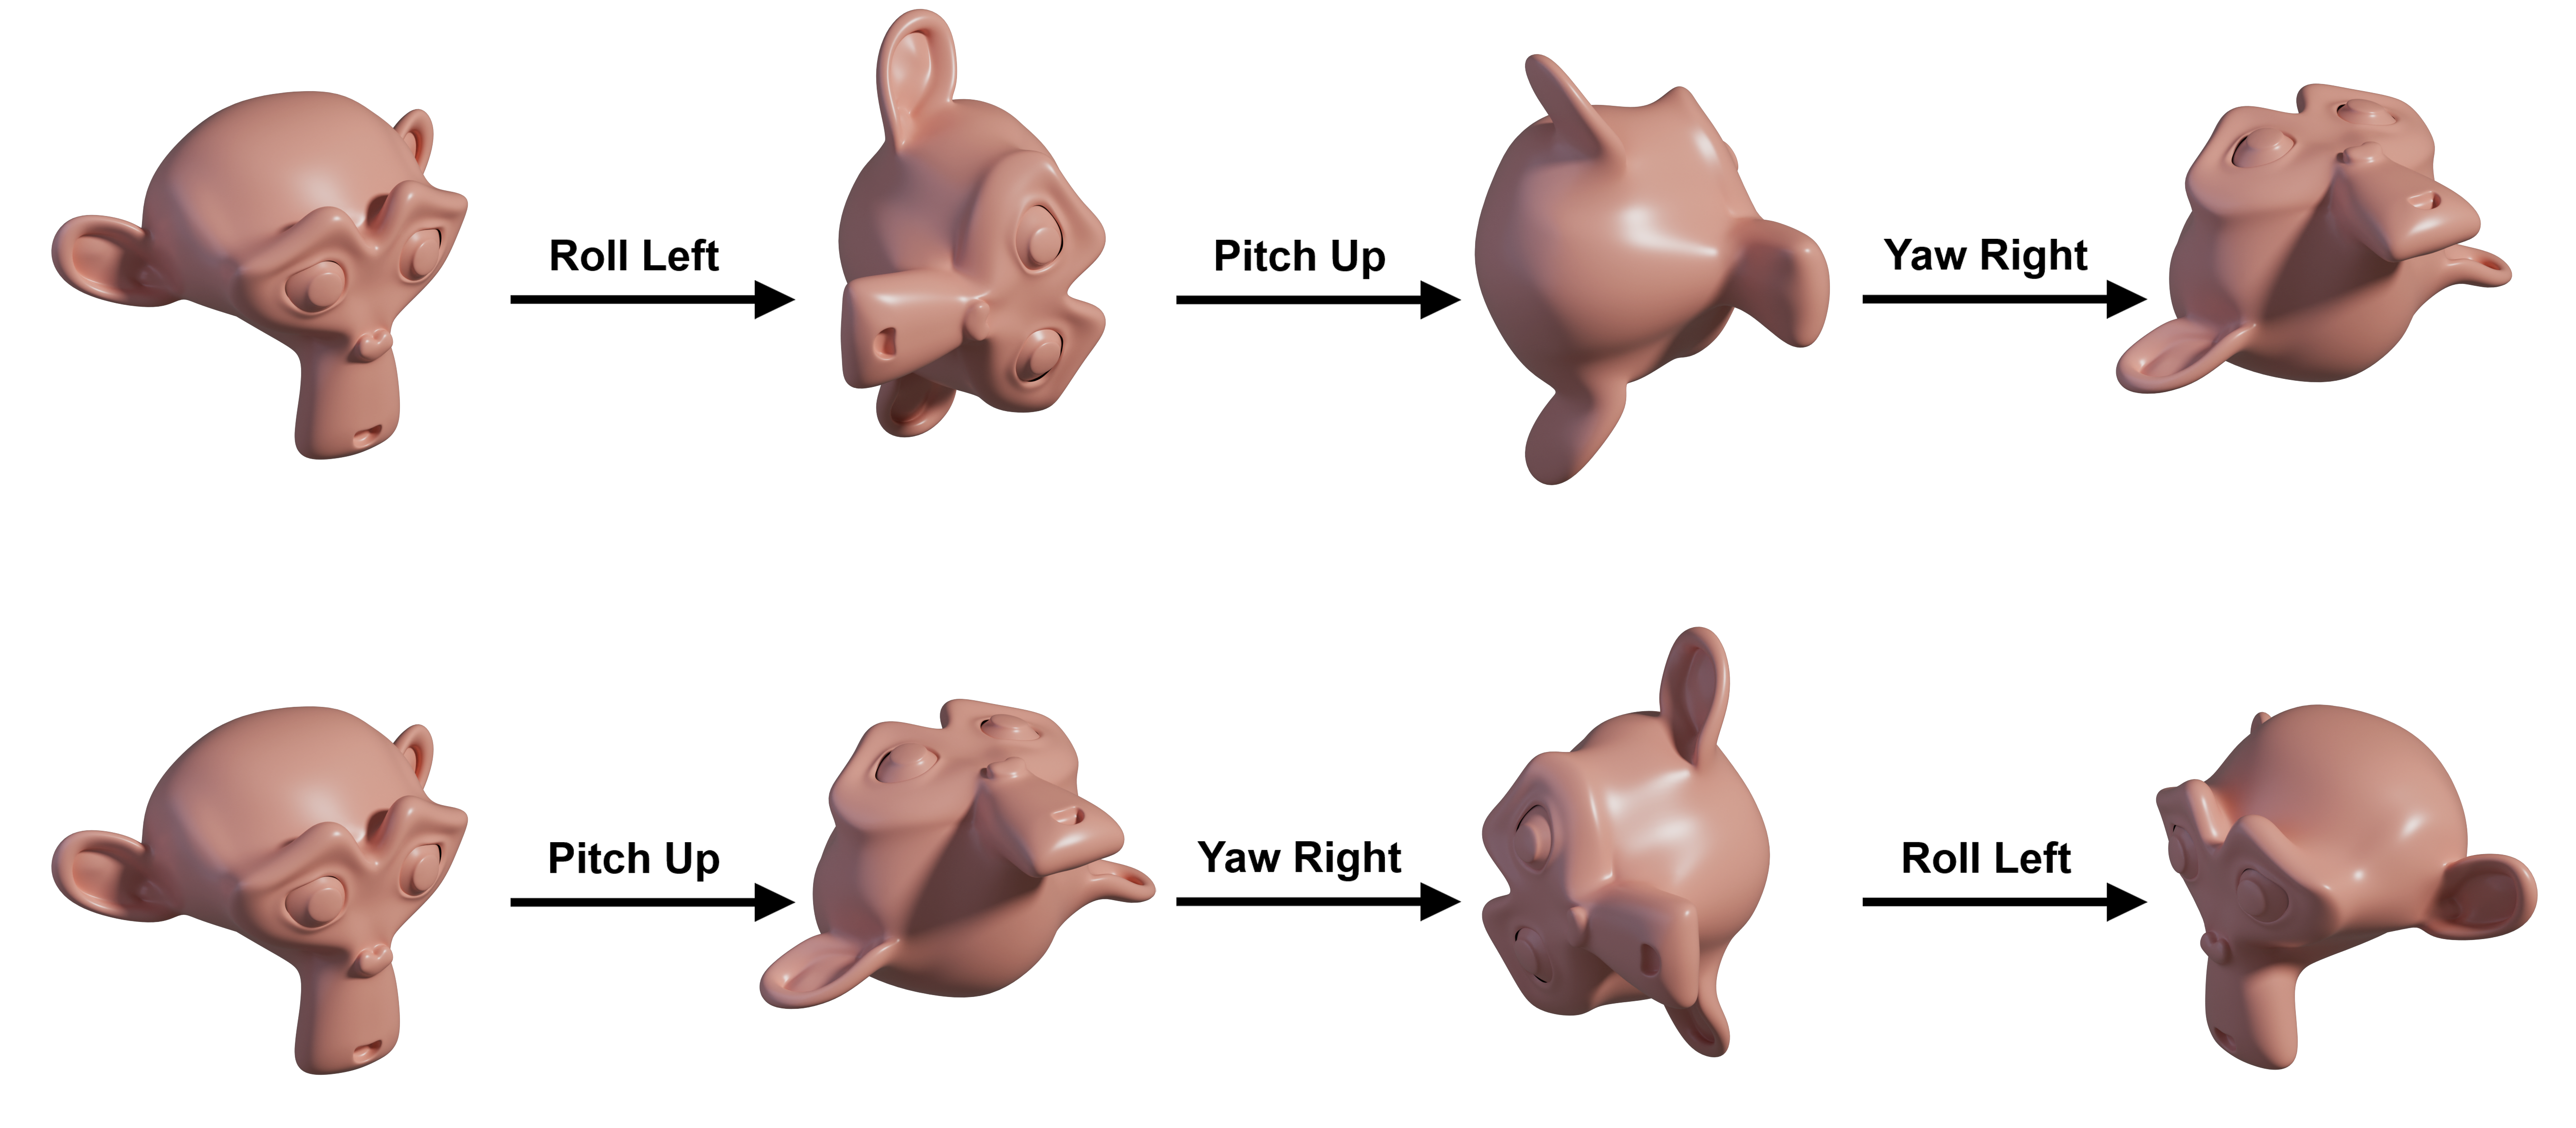
\includegraphics[width=\linewidth]{Images/LargeRotationsExample.png}
        \caption{Example of non-commutative rotation sequences}
        \label{fig:large rot}
    \end{figure}
    As we can see, our monkey, Suzanne, has ended up in very different rotations in either case, even though we performed the same rotation operations. Of course, if you have read Volume II, this is not at all an unexpected result. 

However, something interesting happens if we consider rotations that are small in magnitude. This is best shown visually, which we will do in \autoref{fig:small rot}. Each rotation in this image is only $10\degree$.

\begin{figure}[H]
    \centering
    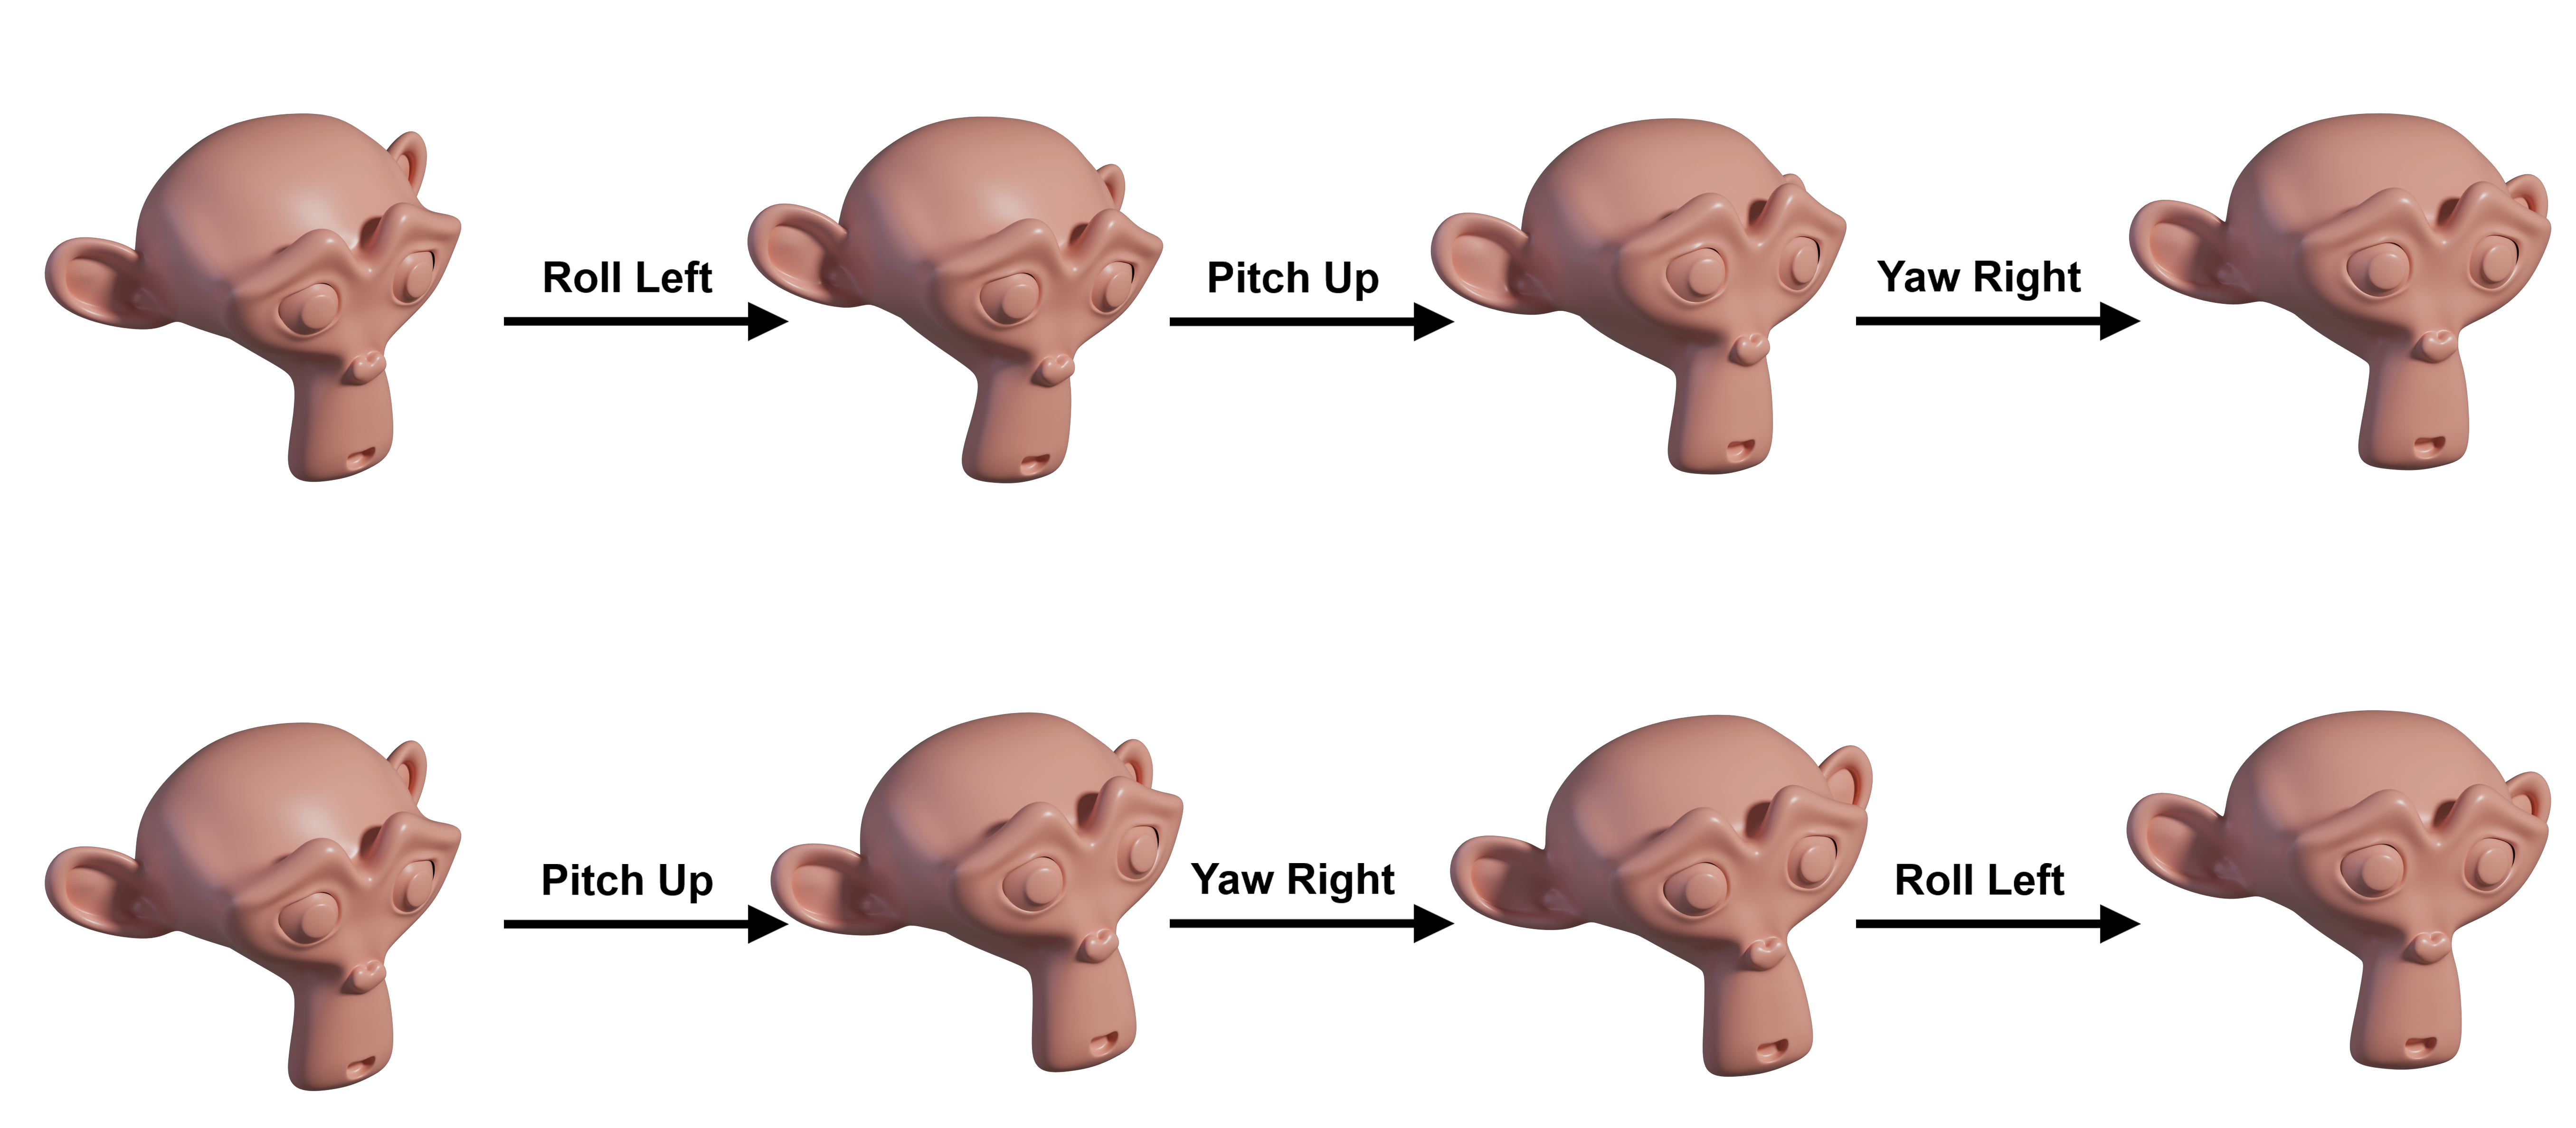
\includegraphics[width=\linewidth]{Images/SmallRotationsExample.png}
    \caption{Example of small rotations being nearly commutative}
    \label{fig:small rot}
\end{figure}
We see that these small rotations yield the same final orientation. Go ahead and try the same rotation sequence with your head! If you choose angles that are fairly small, you will see that you do in fact end up looking in the same spot no matter which rotation sequence you choose! Of course, these two rotations are not \textit{exactly} identical, but they are really close! You can notice some small difference by looking at where Suzanne's' ear intersects with the eyebrow. 

However, these two do seem very similar, which is definitely a different outcome than the large rotations. As we will later prove rigorously, as these rotations get smaller and smaller, these so-called \textit{infinitesimal} rotations will be mathematically identical.

Based on what we've learned from \gls{lie theory} so far, this should give us a few hints as to whats happening. The small rotations are very close to the \gls{lie algebra}, where the elements form a vector space. However, the large rotations exhibit behavior that can only be explained on the manifold. Notice the parallel here with our two dimensional rotations. Even though those two dimensional rotations are commutative and the three dimensional rotations are not, the same principle of infinitesimal rotations holds. The following sections will explain these attributes more mathematically and give special characteristics of rotation groups and algebras.
\end{example}

\subsection{Rotation Groups}
To describe a rotation mathematically, we first need to understand what rotations do. Aside from the obvious fact that rotations `rotate', some properties are inherit no matter what space we rotate in (although 2D and 3D are the most common for us). These properties will help us define the group structure of rotations:

\begin{enumerate}
    \item  Rotations superpose. If we rotate once, and then rotate again, the result is still a rotation, and more importantly, the result is the sum of the first and second rotation.
    \item Secondly, a rotation preserves angles and lengths. By rotating, the length of a vector is never changed. Additionally, the angle between two vectors must also be constant.
    \item Lastly, and likely the most overlooked, rotations preserve the orientations of objects. A pure rotation will never change the order of vectors. This is distinct from a reflection, in which the first two properties hold but the orientation is not preserved.


\end{enumerate}

%Figure for all of these

Each of these have direct mathematical implications. We can go through each of the previously listed properties in order, describing them mathematically:
\begin{enumerate}
    \item The fact that rotations superimpose tells us that a linear representation of then exists -- we can express them in terms of vectors and matrices. Using the other properties, we can ascertain more about the matrix that represents this rotation.
    \item Preserving angles and rotations means that the dot product is constant under a rotation. Assuming that our rotation is denoted $R$, this means that two vectors, $\vec{v}$ and $\vec{w}$ have the following relationship under a rotation:
    \begin{equation}\label{eq:dotty dot prod}
        \vec{v}\cdot \vec{w}=(R\vec{v})\cdot(R\vec{w})
    \end{equation}
    It is known that for real dot products, we can replace the dot product of $\vec{v}\cdot \vec{w}$ with $\vec{v}^\top \vec{w}$ (you can easily prove this to yourself). So, we can rewrite \eqautoref{eq:dotty dot prod} as:
 \begin{equation}
        \vec{v}^\top \vec{w}=(R\vec{v})^\top(R\vec{w})
    \end{equation}
Which can be simplified using the identity that $(R\vec{v})^\top =\vec{v}^\top R^\top $ to:
 \begin{equation}
        \vec{v}^\top \vec{w}=\vec{v}^\top R^\top R\vec{w}
    \end{equation}
For this statement to be true, $R^\top R$ must be equal to the identity matrix, $\mathbb{I}$. The only way this can occur is if:
\begin{enumerate}
    \item R is invertible.
    \item     The transpose of $R$ is it's inverse.
\end{enumerate}
The first statement implies that $R$ must be square (Invertible Matrix Theorem). The second condition that $R^{-1}=R^\top $ is a special condition which implies that the matrix is \textit{orthogonal}. This is a modification of the condition that we saw in \autoref{sec:matrix groups}. In that section, we defined the general linear group $GL(n)$. With the additional constraint that $R^\top =R^{-1}$, we say that rotations exist in the $O(n)$ group. Thus, $O(n) \subset GL(n)$.

    \item The last property is that the orientation and dot products are preserved. Once again, this is the same property that we saw with the special linear group $SL(n)$, and we use the same notation here for the special orthogonal group - denoting it $SO(n)$. As before, the important property with this group is that $\det SO(n) = 1$

\subsection{Rotation Algebras}
    
\end{enumerate}
As mentioned in the introduction to \gls{lie theory}, the \gls{lie algebra} represents the tangent space of the \gls{lie group}. We can intuitively think of the tangent space as taking a derivative. So, we can create our mathematical description of the \gls{lie algebra} for rotations in this way.

We start by taking a differential rotation, one that is very small, which we denote $\varepsilon$. We then use the defining relationship of $O(n)$:
\begin{equation}\label{eq:rotationDef}
    R^\top R=\mathbb{I}
\end{equation}

We can think of $R$ for an infinitesimal rotation. For a very small rotation, the matrix will be only very slightly different from the identity, shifted by some amount $\varepsilon A$, say. Of course, there are some higher order corrections, but choosing $\varepsilon$ to be small, these are insignificant.\endnote{More strictly, we choose $\varepsilon>0$ but so small that $\varepsilon^2=0$. If our rotation is infinitesimal, this is exactly true.} Thus, we can write\endnote{Notice the similarity in this construction and the one for two dimensional rotations we found earlier. We can, in fact, say that this $\varepsilon A$ is the same as the generator matrix which we found for two dimensional rotations.}:
$$R=\mathbb{I}+\varepsilon A$$
The matrix $A$ is representative of the \gls{lie algebra}, the form of which we have yet to define. We can use this relationship in \eqautoref{eq:rotationDef} to find properties of A:
$$(\mathbb{I}+\varepsilon A)^\top (\mathbb{I}+\varepsilon A)=\mathbb{I}$$
We expand the product and ignore any terms with coefficients of $\varepsilon^2$  since these higher order corrections are zero for an infinitesimal transformation. This leads us to:
$$\mathbb{I}+\varepsilon(A^\top +A)=\mathbb{I}$$
From here, the $\mathbb{I}$ matrices cancel, and we are left with the relationship that:
\begin{gather}
    \color{blue}\boxed{\color{black}A^\top =-A}\\
    \color{blue}\mathrm{Skew \ Symmetry}
\end{gather}
This relationship is called \textit{skew symmetry}, and it is the fundamental property of infinitesimal rotations (or the \glspl{lie algebra} of rotations, put another way). One notable feature of skew symmetric matrices is that the diagonal must be zero for the property to hold\endnote{We may identically say that $\det{A}=0$. Remember that for the \gls{lie group}, our determinant was 1, which we may arrive at through $e^0=1$}. We call the \gls{lie algebra} for which this condition holds $\mathfrak{so}(n)$.

We can use the condition on the determinant of the \gls{lie group} to get more information about the \gls{lie algebra}. We know that the determinant of $SO(n)$ must be 1. Therefore, we may have a condition for the $\mathfrak{so}(n)$ \gls{lie algebra} that arises from this. We can use the previously established fact that the trace is related to the matrix exponential determinant (see \autoref{exer:trace det} for more information):
$$e^{tr(A)}=\det\left(e^A\right)$$
The matrix $A$ is the \gls{lie algebra}, and thus $e^A$ is the exponential map, such that $e^A$ is the \gls{lie group}. We have previously determined that the $SO(3)$ \gls{lie group} must have determinant 1, so the equation is:
$$e^{tr(A)}=1$$
Solving the equation by taking the logarithm of both sides, we have:
$$tr(A)=0$$
This condition implies that all of the elements of the diagonal must add to zero! A matrix with such a property is called traceless. Using the other criteria that $A^\top =-A$, each diagonal entry of this matrix must be 0.

The \gls{lie algebra} of the rotation groups appears quite often in engineering and physics. Anytime an infinitesimal rotation must be described a skew symmetric matrix is often associated with it! One example you may remember is the quaternion integration equation from Volume I:
$$\dot{\textbf{q}}=\frac{1}{2}\begin{bmatrix}
        0&-\omega_x&-\omega_y&-\omega_z\\
        \omega_x&0&\omega_z&-\omega_y\\
        \omega_y&-\omega_z&0&\omega_x\\
        \omega_z&\omega_y&-\omega_x&0
    \end{bmatrix}\vec{q}$$
As we can see, this matrix has the properties of the \gls{lie algebra} of rotations! It is skew-symmetric and has a trace of 0.

\subsubsection{The Cross Product and Euler Vector}

Having described the form of the rotation group and the rotation algebra in the context of \gls{lie theory}, we can move on to describing these elements in the more familiar context.



One of the simplest cases in showcasing the relationship between the \gls{lie group} and the \gls{lie algebra} is the rotation.

Starting with an infinitesimal rotation, which is a group in $\mathfrak{so}(3)$, we have:
$$A=\begin{bmatrix}
    0 &-\omega_z & \omega_y \\
    \omega_y & 0 & -\omega_x \\
    -\omega_y & \omega_x & 0
\end{bmatrix}$$

We can use the \gls{exponential map} to go from the \gls{lie group} to the \gls{lie algebra}. For matrices, we use the matrix exponential as the \gls{exponential map}. Performing the exponentiation, we have that $e^{A}$ is a rotation matrix.

\subsubsection{Visualization of SO(3) Rotations}


\subsection{Revisiting the BKE}
We can use \gls{lie theory} in order to describe the \gls{bke} in another way. 
Explain the \gls{bke} in terms of \gls{lie theory}.

\section{Complex Rotations and Spinors}
Until now, we have not discussed complex-valued matrices. However, these find use in physics quite often and we can even parameterize the quaternions in terms of complex matrices. We will now explore these complex matrices to gain an understanding of more complex matrix transformations, which are beyond the 3-D rotations we have discussed so far. These ideas will help us relate the quaternions to rotations and understand how $SU(2)$ and $SO(3)$ space are linked!

This section summarizes some of the ideas that are presented in the \cite{eigenchris_spinors_nodate} playlist of videos.

We may start by considering the 




\section{Physics Applications of Lie Theory}

\subsection{Quantum Mechanics}
\color{red} All quantum mechanical operators are elements of lie algebras! \color{black}

\subsection{Spinors}



\section{Relation to Differential Equations}\label{sec:lie theory relation to differential equations}
We noted in the beginning of this chapter that \gls{lie theory} was originally developed to solve differential equations. We can return back to this example to help us tie the theory into math that almost every engineer has studied extensively.

The foundation of differential equations is, quite naturally, the derivative. Thus, we can start our discussion by showing how the derivative is related to the \gls{lie algebra}.

\subsubsection{Relation to derivatives}
We will start this discussion with the ordinary total derivative that is taught in introductory calculus classes in the context of \gls{lie theory}. Our goal here is to show that the Jacobi identity may arise somewhat naturally by considering the derivative product rule:
$$[f(x)g(x)]'=f(x)g'(x)+f'(x)g(x)$$

Starting with the Jacobi identity, which we know all \glspl{lie algebra} must satisfy, we have:

which can otherwise be expressed as:
$$[x,[y,z]]=-[y,[z,x]]-[z,[x,y]]$$
We have also shown that the Lie bracket is alternating, so we can remove the negative signs on the RHS simply by changing the order of the bracket:
$$[x,[y,z]]=[y,[x,z]]+[[x,y],z]$$

We can rewrite this expression by considering an operation, $D$, which is defined $D(\xi)=[x,\xi]$. Applying this to the equation below, we have:
$$D([y,z])=[y,D(z)]+[D(y),z]$$
Since we consider the Lie bracket to be a type of multiplication, we can write the above formula as:
$$D(yz)=yD(z)+D(y)z$$
Which matches the result of the product rule exactly!

\subsubsection{Differential Equations}
\begin{example}[Matrix Differential Equations]
    Since we have been studying matrix groups, let us consider the class of first order matrix differential equations. We see these systems frequently in control theory so it is good to study them here.
    $$\dot{x}=Ax$$
    Where $A$ is an $n{\times}n$ matrix with constant coefficients and $x$ and $\dot{x}$ are $n{\times}1$ vectors. We can find the solution of this equation through separation and integration. We start by performing the seperation of variables:
    $$\frac{dx}{x}=Adt$$
    We can this integrate this equation to find the solution.
    $$\int_{x_0}^x{\frac{dx}{x}}=\int_{t_0}^\top {Adt}$$
    So, we have $\ln\left(\frac{x(t)}{x_0}\right)=A(t-t_0)$. We note that $t-t_0$ can be replaced by $\Delta t$. Finally, we exponentiate to arrive at our solution to the differential equation:
    \begin{gather}
        \color{blue}\boxed{\color{black}x(t)=e^{A\Delta t}x_0}\\
        \color{blue}\mathrm{Solution \ of \ } \dot{x}=Ax        
    \end{gather}
We can see the presence of the matrix exponential $e^{At}$, which we have seen before when discussing the \gls{lie theory} of matrices! This is an important connection to make, so let us expand on it for clarity.

    Generally, in control theory, we may denote $e^{At}$ (or $e^{A\Delta t}$, they are practically the same) as the \textit{state transition matrix}, which is sometimes denoted $\Phi$. This state transition matrix will extraordinarily important when we discuss concepts such as Kalman filtering.

    So why does it appear here, and how can we relate that to our discussion of \gls{lie theory}?

    We can think of it in the following way. Our matrix $A$ represents infinitesimal behavior of the system. That's why $\dot{x}$ is described in terms of $A$! It tells us how the parameters vary on an infinitesimal scale. The matrix exponential $e^{At}$, is effectively a map from this infinitesimal solution to a finite time solution; that is, something we can measure.

    In \gls{lie theory} we have the exact parallel behavior. We have some tangent group on the \gls{lie algebra}, which is mapped onto the group element by the exponential map!

    We can see that these two descriptions are very similar! The key difference is that \gls {lie theory} can describe groups which are non-linear, which makes is a more powerful tool than solving a linear differential equation.
\end{example}

\section{Lagrangian and Hamiltonians on Manifolds}

\section{Noether's Theorem}\label{Noether's Theorem}

We touched on this briefly in \autoref{sec:motivation and background lie}, but in many physical problems (and in \gls{lie theory}), we are concerned with physical symmetries. Noether's Theorem states the following:

\begin{theorem}[Noether's Theorem]
In a system that can be modeled purely by a Lagrangian (that is, a conservative system), every continuous symmetry has a corresponding conservation law.
\end{theorem}
The implications of this statement are quite great. Noether's Theorem gives us a pathway to understand where the conservation laws of symmetry actually come from. Of course, we can also reverse the statement and understand the symmetries of our system based on the conserved quantities!

Although we have discussed continuous symmetries quite a bit in our discussion of \gls{lie theory}, concrete examples will aid us greatly.

\subsection{Conservation in Physics}

Before we get started, we should concretely define the terminology of the theorem. What exactly do we mean by a conserved quantity?

A conserved quantity is simply one that does not change over time. When we say that energy is conserved, we mean that the energy of the system will be exactly the same if observed at $t=0\ \mathrm{s}$ or $t=100\ \mathrm{s}$. If we call our quantity of interest $X$, we can express this as:
$$\frac{dX}{dt}=0$$

\subsection{Symmetries in Physics}
As we have discussed earlier, the picture of groups and symmetries changes a bit between each domain of math or physics that we are discussing. In the domain of physics, our picture of symmetries is most definitely different than the picture of triangles or number lines.

When we discuss a symmetry in physics, we mean to say that the physics that act upon that system are in no way altered by whatever transformation we have performed (that is to say, the \gls{eom} is identical).

For example, if we decide to move our rocket launch 20 ft to the north, the aerodynamics, gravity, and forces of the rocket are still exactly the same. We have performed a transformation -- in the form of moving the launch location -- but there are no observable differences to the system!

Of course, these transformations are not merely limited to physical movements of the system, there are other types of transformations that we can do that do not impact the physics of the system.

\subsection{The Mathematical Formulation}

We know from Hamilton's Principle that physical trajectories have an action of zero. We denote this action as $S$, and the path it follows as $\gamma$, so we may write $S[\gamma]=0$. It may be possible to find another path $S[\gamma_2]=0$ somewhere else along the state space. This is not particularly noteworthy. We can take the analogy of the derivative from calculus as an example in \autoref{fig:calc sym}:
\begin{figure}[H]
    \centering

\tikzset{every picture/.style={line width=0.75pt}} %set default line width to 0.75pt        

\begin{tikzpicture}[x=0.75pt,y=0.75pt,yscale=-1,xscale=1]
%uncomment if require: \path (0,300); %set diagram left start at 0, and has height of 300

%Shape: Polynomial [id:dp5733809673289914] 
\draw  [line width=1.5]  (100,225) .. controls (170,35) and (240,320) .. (310,130) ;
%Shape: Polynomial [id:dp22075841317731382] 
\draw  [line width=1.5]  (310,130) .. controls (383.33,-100) and (456.67,245) .. (530,15) ;
%Straight Lines [id:da16902943176946206] 
\draw [color={rgb, 255:red, 74; green, 144; blue, 226 }  ,draw opacity=1 ][line width=1.5]    (210,199) -- (290,199) ;
%Straight Lines [id:da8215493758509421] 
\draw [color={rgb, 255:red, 74; green, 144; blue, 226 }  ,draw opacity=1 ][line width=1.5]    (430,99) -- (510,99) ;
%Straight Lines [id:da24241399926680518] 
\draw [color={rgb, 255:red, 218; green, 44; blue, 0 }  ,draw opacity=1 ]   (320,95) -- (280,65) ;
%Straight Lines [id:da37036162717673604] 
\draw [color={rgb, 255:red, 218; green, 44; blue, 0 }  ,draw opacity=1 ]   (400,240) -- (468.58,112.64) ;
\draw [shift={(470,110)}, rotate = 118.3] [fill={rgb, 255:red, 218; green, 44; blue, 0 }  ,fill opacity=1 ][line width=0.08]  [draw opacity=0] (8.93,-4.29) -- (0,0) -- (8.93,4.29) -- cycle    ;
%Straight Lines [id:da8857104314835499] 
\draw [color={rgb, 255:red, 218; green, 44; blue, 0 }  ,draw opacity=1 ]   (350,250) -- (262.74,211.22) ;
\draw [shift={(260,210)}, rotate = 23.96] [fill={rgb, 255:red, 218; green, 44; blue, 0 }  ,fill opacity=1 ][line width=0.08]  [draw opacity=0] (8.93,-4.29) -- (0,0) -- (8.93,4.29) -- cycle    ;
%Straight Lines [id:da5379556180362811] 
\draw [color={rgb, 255:red, 74; green, 144; blue, 226 }  ,draw opacity=1 ]   (250,199) ;
\draw [shift={(250,199)}, rotate = 0] [color={rgb, 255:red, 74; green, 144; blue, 226 }  ,draw opacity=1 ][fill={rgb, 255:red, 74; green, 144; blue, 226 }  ,fill opacity=1 ][line width=0.75]      (0, 0) circle [x radius= 2.34, y radius= 2.34]   ;
%Straight Lines [id:da1048842221660955] 
\draw [color={rgb, 255:red, 74; green, 144; blue, 226 }  ,draw opacity=1 ]   (470,99) ;
\draw [shift={(470,99)}, rotate = 0] [color={rgb, 255:red, 74; green, 144; blue, 226 }  ,draw opacity=1 ][fill={rgb, 255:red, 74; green, 144; blue, 226 }  ,fill opacity=1 ][line width=0.75]      (0, 0) circle [x radius= 2.34, y radius= 2.34]   ;

% Text Node
\draw (354,242.4) node [anchor=north west][inner sep=0.75pt]  [color={rgb, 255:red, 218; green, 44; blue, 0 }  ,opacity=1 ]  {$f'=0$};
% Text Node
\draw (249,47.4) node [anchor=north west][inner sep=0.75pt]  [color={rgb, 255:red, 218; green, 44; blue, 0 }  ,opacity=1 ]  {$f( x)$};


\end{tikzpicture}

    
    \caption{Calculus Analogy of Discrete Symmetry}
    \label{fig:calc sym}
\end{figure}
Given a general function, it is expected that there will likely be multiple minima, separated spatially. What Noether's Theorem is concerned with is infinitesimal transformations that do not change the action at all. In the case of our example before, we have some transformation, which we may call $T$, which maps path $\gamma$ to $\gamma'$:
$$\gamma\xrightarrow{T}\gamma'$$
When we have a continuous symmetry between these two, there is no difference in the action! So $S[\gamma]=S[\gamma']$.

\section{The Limitations of Lie Theory}
A fundamental understanding of the mathematics that relate groups and algebras is quite interesting, but ultimately, our goal in engineering is to be able to control a system which is not mathematically ideal. We will have disturbances and random behaviors and noisy sensors in all of our real systems. Do these non-idealities make \gls{lie theory} useless for us? Of course not, but it does impose limitations of the extent to which we can use it.

It is best to think of \gls{lie theory} as a tool that we can use to understand the relationships between infinitesimal elements and the larger system behavior that we see. From \gls{lie theory}, we can derive a large number of theoretical conclusions (and some which are still active research!) which prove useful to us. Understanding where our theoretical results come from can help us to understand new systems and generate methods of tackling difficult problems. That alone makes \gls{lie theory} a topic worth serious exploration.

Lie Theory, however, is not a silver bullet which can solve all of our practical problems. Quite notably, the computation of matrix exponentials and general exponential functions can be quite expensive and unintuitive, so it often cannot be used in real time systems. From here, we will use \gls{lie theory} mostly to contextualize some of the background and behind the scenes mathematics. 

\newpage

\printendnotes


\chapter{Symplectic Integrators}\label{sec: Syplectic Ints}
In addition to the standard \gls{numerical int} schemes explored in Volume I, there are a variety of integration schemes that use energy conservation as the basis of their integration schemes. These types of integrators are called \glspl{symplectic int} and \glspl{variational int}. These types of integrators directly solve Hamilton's equations for a \gls{Hamiltonian} system. The form of these equations is discussed in \autoref{chap:hamiltonian}.

Because the \gls{Hamiltonian} equations are first order already, they are ready for numerical integration without the need for order reduction.

A similar operation can be done to reduce the \gls{Lagrangian} to two first order equations, in a system known as a variational integrator.

MATLAB has no built in functions for variational or \glspl{symplectic int}, so to implement them we need to discuss their properties in full. 

\section{The Mathematical Background}
Our discussion will build off the mathematical discussion of the \gls{lie group}, so a thorough reading of \autoref{chap:lie theory} is recommended. We will use properties of the $SL(n)$ group as well as some new features.

We will construct a group called the \textit{Symplectic Linear Group} to do this. We define the group as follows:
\begin{gather}
    Sp(2n)\equiv\left\{\psi\in GL(2n,\mathbb{R})|\psi^\top \Omega\psi=\Omega\right\}\\
    \mathrm{where  \ } \Omega=\begin{bmatrix}
        0&I(n)\\-I(n)&0
    \end{bmatrix}
\end{gather}
We can deconstruct the meaning of the line to be: The symplectic linear group is a group, such that set $\psi$, which is a subset of the general linear group $GL(2n,\mathbb{R})$, satisfies the property that $\psi^\top \Omega\psi=\Omega$.

Moreover, $Sp(2n)$ is a \gls{lie group}!


\section{Implementation}


\subsubsection{Use Case of Symplectic Integrators}
Although MATLAB does not have built-in functions for these integrators, scripts to do so can be written or found online.

The best use case for these algorithms is for systems with a \gls{Hamiltonian} or \gls{Lagrangian} description that need to be integrated over a long time span. Because these integrators conserve energy, they will better preserve the characteristics of these systems over long times as compared to RK integrators.

\chapter{The Lebesgue Integral and Measure}

\begin{chapquote}{Andrew Lewis}
``The Lebesgue theory of integration is to the Riemann theory of integration as the real numbers are to the rational number''
\end{chapquote}

In the interest of keeping \autoref{part:control theory} free of too much strictly mathematical content, I have devised this chapter which contains much of the math which is foundational in classical control theory.

For the reader interested in the mathematics behind inner product spaces, I have included some supplemental information on the Lebesgue integral, which is the mathematical construction that is used to rigorously define inner product spaces.




\section{Field Theories}

To describe field theories, we should first return to the \gls{Lagrangian} which we have discussed earlier. So far, we have discussed discrete systems. That is, systems which we can describe with a finite number of degrees of freedom.

What happens if we instead try to model something which is continuous? In our applications, we can approximate any fluid as continuous. In physics, gravitational fields and electromagnetic fields are continuous. 

\chapter{A Brief Tour of Complex Analysis}
\begin{chapquote}{Jacques Hadamard}
    The shortest path between two truths in the real domain passes through the complex domain.
\end{chapquote}


\chapter{Tensor Operations}
Before we dive into differential geometry or any of the related topics, we must first have a good understanding of tensors and their operations.

\chapter{Differential Geometry}
Differential geometry is a field of study that is concerned with the study of smooth manifolds - which essentially means that it is an object which `looks' like a vector space when viewed closely. The subject of differential geometry was lightly touched upon in \autoref{ex:geodesic}, where we considered the shortest path on a spherical surface. In \autoref{ex:geodesic}, we showed this property on the sphere, but differential geometry allows us to study any manifold, so long as it is smooth! 

As we have seen, smooth manifolds are quite important to \gls{lie theory}, and many other applications as well. It is thus sagacious to devote a chapter to a study of differential geometry. We find that many physical systems can be described by the methods of differential geometry.

We can think of a manifold as anything which we can continuously parameterize. So, our 3D rotations that we parameterize with Euler angles or quaternions are also elements of a manifold. We also see that manifolds are also useful in \gls{Lagrangian} and \gls{Hamiltonian} mechanics in the form of \textit{symplectic manifolds}.

So, this is a field of study that touches upon many of the mathematical concepts that we encounter in the study of dynamics and control theory. While not strictly necessarily, a preliminary understanding of manifolds will prove useful for further study. Moreover, those readers interested in physics will find many uses for the topics of discussion here.

This chapter will take an approach closer to physics rather than pure math, as the math requires knowledge of topology and analysis which are well outside the scope of this book and the expected knowledge of the target audience. However, useful information and a working knowledge of the subject can be gained nonetheless from a slightly less -- but still informative -- approach to the subject.

\section{Invariance, Covariance \& Contravariance }

Change of basis and change of component matrices are inverses of each other. Seen with scaling, rotations, etc.

Quantities that act in the opposite direction as the basis vectors are contravariant, those that act the same are covariant. There \textbf{must} be an inverse relationship between covariant and contravariant quantities to maintain the same value. 

Quantities which are unchanged are invariant. Tensors are invariant quantities! Can be described differently, but the properties never change

covariant - row
contravariant - column


\subsection{The Metric Tensor}
The concept of a metric is of upmost importance to differential geometry. A metric space is a set with a notion of a distance.

The most typical metric space is the Euclidean $\mathbb{R}^2$ space. The distance in this space is perhaps the most famous distance formula to exist:
$$s=\sqrt{x^2+y^2}$$

\subsection{Distances}
We can generalize the concept of the Euclidean distance, which we typically define as
$$s=\sqrt{x^2+y^2}$$
In a generic metric space, we can define this as
$$s=\int_a^b\sqrt{g_{ij}\frac{dx^i}{d\lambda}\frac{dx^j}{d\lambda}}d\lambda$$
\subsubsection{Applying Euler-Lagrange}
We notice that the form of the equation for the arc-length matches the form of a functional in \gls{Lagrangian} mechanics! We can apply the Euler-Lagrange equation to get a general equation for the geodesic on any surface!

$$\frac{d^2x^i}{d\lambda^2}+\Gamma_{mn}^i\frac{dx^m}{d\lambda}\frac{dx^n}{d\lambda}=0$$

\section{The Lie Derivative}




\section{Special Relativity}

\section{General Relativity}

\chapter{Geometric Control}



\chapter*{The End!}
And so, you have finished all three volumes of the Flight Dynamics Bible! This is quite the accomplishment. In this volume, you have read over 60,000 words and 2000 equations. Throughout the series, that is more than 100,000 words spanning many semesters of content.

Preston and I hope that this series has been beneficial to you and furthered your knowledge of flight dynamics and all other subject enclosed. Of course, this reading is only the beginning of your journey. From here, there are many avenues that you can explore - be that \gls{gnc}, avionics, robotics, physics, or otherwise.

My hope is that the reader have derived from these books some useful intuition for these complex topics and are inspired to study further. There is a vast amount of knowledge to be gained, and so much fundamental beauty in studying the math and physics of the natural world. I will leave you with one final quote as you continue your journey. 

\begin{chapquote}{Yo-Yo Ma}
``The worst thing you can do is say to yourself, `I want to be just like somebody else.' You have to absorb knowledge from someone else, but ultimately you have to find your own voice.''
\end{chapquote}

If you have any suggestions for improvements to these books, please message me on slack @HudsonReynolds or reach out by email at HudsonJ.Reynolds@gmail.com. Thank you for reading.

\appendix
\addappheadtotoc

\renewcommand{\chaptername}{Appendix}
\renewcommand{\chapterautorefname}{Appendix}

\chapter{Methods of Matrix Exponentiation}\label{sec: computation of matrix exp}

The exponentiation of matrices prove to be extremely useful in many of the applications here. There are several ways to approach the matrix exponential, with each having their own advantages in approach. We will start with the simplest to construct and move to more complex (although sometimes better!) approaches.

\section{Matrix Exponential as Taylor Series}
Expressing the Matrix Exponential as a Taylor series is the simplest definition we can use, although a closed form only exists in limited cases. Such as an example is:
$$A=\begin{bmatrix}
    0&1&1\\0&0&1\\
    0&0&0
\end{bmatrix}$$
For this matrix, we can take the Taylor series directly to find $e^A$.
\begin{equation}\label{eq:eA taylor series}
    e^A=\sum_{n=0}^2{\frac{A^n}{n!}}=A^0+A+\frac{A^2}{2}
\end{equation}

Although it may not be immediately apparent why we can stop the sum at $n=2$, it becomes immediately apparent upon computation. We have:
$$A^0=\mathbb{I},A=\begin{bmatrix}
    0&1&1\\0&0&1\\
    0&0&0
\end{bmatrix},A^2=\begin{bmatrix}
    0&0&1\\0&0&0\\
    0&0&0
\end{bmatrix},A^3=\begin{bmatrix}
    0&0&0\\0&0&0\\
    0&0&0
\end{bmatrix}$$
So, $A^3$ and any successive derivative is exactly zero, so the sum is finite. So, the computation simply becomes addition of the matrices, giving us:
$$e^A=\begin{bmatrix}
    1&1&\frac{3}{2}\\0&1&1\\
    0&0&1
\end{bmatrix}$$
This closed form only exists for simple matrices. We can extend this \textit{slightly} for some some matrices, as we can separate $e^A$ into $e^{(A+B)}=e^Ae^B$ in the case that $AB=BA$ (otherwise known as $A$ and $B$ \textit{commuting}). This is generally not the case so we will not dive further.

The reason to present this method is that sometimes the other methods I will present to perform matrix exponentiation will not always work. In that case, when computing the matrix exponential, it is often okay for our purposes to find a `close enough' value by taking some finite sum of the Taylor series expansion. This method will always work; we all remember from introductory calculus that $\sum_{n=0}^\infty{\frac{A^n}{n!}}$ is an absolutely convergent series.

\section{Matrix Exponential as Eigenvalue Decomposition}
The next method will likely be familiar to students of linear algebra. This method involves taking the eigenvalue decomposition of the matrix $A$ to find its exponential. Diagonalization Theorem (presented in \autoref{thm:diagonalization thm}) tells us that we can only perform this diagonalization if $A$ has $n$ linearly independent eigenvectors. We can easily check this in MATLAB with the command "[P,D]=eig(A)", which returns the eigenvector matrix "P" and diagonalized matrix "D". We will not cover how to derive these matrices here. If you want a derivation, a good high-level overview is presented in \cite{michael_penn_matrix_2022}.

\begin{theorem}[Diagonalization Theorem]\label{thm:diagonalization thm}
    An $n{\times}n$ matrix $A$ is diagonalizable if and only if $A$ has $n$ linearly independent eigenvectors.
\end{theorem}

When we satisfy these criteria, we can write the matrix $A$ as $A=PDP^{-1}$.\endnote{You may see this decomposition as either $A=PDP^{-1}$ or $A=P^{-1}DP$. This distinction depends on how you choose to represent $P$. I choose to use the notation that allows users to use write the given equations in MATLAB directly. This is also the standard notation in most modern textbooks.} This becomes useful when computing the matrix exponential. Why exactly is this useful if we now have more terms?

\begin{example}[$A^2$ for diagonalizable matrices]
    We can take the example of $A^2$ for a general matrix $A$ with the decomposition $A=PDP^{-1}$ to show the usefulness. 
    
We start by squaring both sides of the equality $$A^2=\left(PDP^{-1}\right)^2$$ which we can expand to $$A^2=PDP^{-1}PDP^{-1}$$
We notice that the middle term, $P^{-1}P$, reduces to $I$, so the sum is simply $$A^2=P(DID)P^{-1}$$which we can express plainly as $$A^2=PD^2P^{-1}$$
\end{example}

We can notice that for any integer $n$, the middle terms $P$ and $P^{-1}$ will cancel each other, given us the general formula:
\begin{gather}
    A^n=PD^nP^{-1}
\end{gather}
We also notice that it is remarkably simple to find $D^n$ since $D$ is a diagonal $n{\times} n$ matrix. We  have:
$$D^n=\begin{bmatrix}
    {d_{11}}^n &0&\cdots&0\\
    0 &{d_{22}}^n & \cdots &0\\
    \vdots & \vdots & \ddots & 0\\
    0&0&0&{d_{nn}}^n
\end{bmatrix}$$
From here it is simple to extent this to the matrix exponential. We can refer back to our original form for the matrix exponential in \eqautoref{eq:eA taylor series} and rewrite is slightly for the diagonalized matrix:
$$e^A=\sum_{n=0}^{\infty}{\frac{1}{n!}A^n}=P\sum_{n=0}^{\infty}{\frac{1}{n!}D^n}P^{-1}$$
We can see that ${\frac{1}{n!}D^n}$ will simplify greatly since $D^n$ has a closed form. We can use the Taylor series definition to get:
$$\sum_{n=0}^{\infty}\frac{1}{n!}D^n=\begin{bmatrix}
    e^{d_{11}} &0&\cdots&0\\
    0 &e^{d_{22}} & \cdots &0\\
    \vdots & \vdots & \ddots & 0\\
    0&0&0&e^{d_{nn}}
\end{bmatrix}=e^D$$
So we have a quite simple way to express the matrix exponential for diagonalizable matrices:
$$e^A=Pe^DP^{-1}$$
\begin{exercise}[Show $e^{tr(A)}=\det\left(e^A\right)$]\label{exer:trace det}
    To ensure that you understand this method of computing the matrix exponential, show that $e^{tr(A)}=\det\left(e^A\right)$ for the matrix: $$A=\begin{bmatrix}
        4&1\\2&5
    \end{bmatrix}$$
    Bonus points are awarded if you can prove this property holds for a general diagonalizable matrix $A$! You will want to use the properties of the trace and determinant on eigenvalues. This property will prove useful when we study rotation groups, so keep it in your back pocket!
\end{exercise}

\section{Matrix Exponential with Jordan Forms}
Eigenvalue decomposition is a very promising method for computing the matrix exponential, but it is not always feasible, since our matrices are not always diagonalizable. In such a case, we may use what is called the \textit{Jordan Normal form} (sometimes called \textit{Jordan Canonical Form}) to compose a pseudo-diagonal matrix and compute the matrix exponential.

\section{Matrix Exponential with Laplace Transform}

There is one more method that we will employ to compute the matrix exponential, which comes from the \gls{laplace transform} which we explored in \autoref{part:control theory}. We may recall that we have:
$$e^{at} = \mathscr{L}^{-1}\left(\frac{1}{s-a}\right)$$
As we have done for our other cases, we can extend this definition to matrices:
$$e^{At} = \mathscr{L}^{-1}\left(\left(s\mathbb{I}-A\right)^{-1}\right)$$
Note that the $\mathscr{L}^{-1}$ of a matrix is the $\mathscr{L}^{-1}$ of each of its elements.

\begin{example}[Diagonal Matrix]
Let's consider a simple example of a diagonal matrix:
$$A=\begin{bmatrix}
    a&0\\0&d
\end{bmatrix}$$
We can compute $s\mathbb{I}-A$:
$$s\mathbb{I}-A=\begin{bmatrix}
    s-a&0\\0&s-d
\end{bmatrix}$$
For a diagonal matrix, our inverse is the reciprocal of the diagonal elements:
$$\left(s\mathbb{I}-A\right)^{-1}=\begin{bmatrix}
    \frac{1}{s-a}&0\\0&\frac{1}{s-d}
\end{bmatrix}$$
For the matrix exponential, we take the \gls{laplace transform} of each element:
$$e^{At}=\begin{bmatrix}
    \mathscr{L}^{-1}\left(\frac{1}{s-a}\right)&0\\0&\mathscr{L}^{-1}\left(\frac{1}{s-b}\right)
\end{bmatrix}$$
Computing this, we have:
$$e^{At}=\begin{bmatrix}
    e^{at}&0\\0&e^{bt}
\end{bmatrix}$$
Which matches our expectation for the result. 
\end{example}
\begin{exercise}[Skew Matrix]
    Use the \gls{laplace transform} method of matrix exponentials to find the matrix exponential of the following skew matrix:
    $$\theta\mathcal{J}=\begin{bmatrix}
        0&\theta\\-\theta&0
    \end{bmatrix}$$
Next, compute the eigenvalues of $\theta\mathcal{J}$ and the eigenvalues of $e^{\theta\mathcal{J}}$. How are the two related? 
\end{exercise}

\section{Computational Methods of Matrix Exponentiation}
Often, we would like to use computers to aid us in the computation of matrix exponentials. In MATLAB, there are several commands which we may use to aid us in computation.

If our computation is purely numeric, we may perform a numerical version of the matrix exponential using "expm(A)", where "A" is our square matrix of interest. Note that "exp" in MATLAB will compute the exponential of each element of the matrix, \textit{not} the exponential for the matrix as a whole.

If we desire a symbolic solution, "expm" may be used on a symbolic matrix. To declare a symbolic variable, we use "syms" followed by each variable we want to declare (e.g. "syms theta x y z").

In addition to these commands, there are several which are useful when performing derivations via the previously mentioned methods:
\begin{itemize}
    \item "[V,J] = jordan(A)" - convert matrix "A" into the Jordan form, "V" returns the generalized eigenvectors and "J" the matrix in Jordan form
    \item "F = laplace(f)" - perform the \gls{laplace transform} of "f".
    \item "f = ilaplace(F)" - perform the inverse \gls{laplace transform} of "F".
    \item "[V,D] = eig(A)" - compute the diagonal matrix ("D") and the eigenvector matrix ("V") for "A". 
\end{itemize}

\chapter{Inner Product Space Examples}\label{sec:inner prod ex}
To solidify the idea of the inner product space, we should consider several inner product spaces that we see quite frequently. These are supplemental inner product spaces that may aid in our understanding of the \gls{laplace transform}.

\section{Fourier Series}
First, lets consider one of the most prominent and simple cases of an inner product space. This inner product space will serve as a basic example which we can use to understand the other inner product spaces.

The Fourier series is a way of representing any periodic function in terms of $\sin$ and $\cos$ components. Sometimes, we may see this more compactly expressed as an exponential of form $e^{i\theta}$. Either way, we are trying to express some function in terms of periodic components. We can, for example, express a square wave using these $\sin$ and $\cos$ components, which is shown in \autoref{fig:fourier}.

\begin{figure}
    \centering
    \includesvg[width=.5\linewidth]{Images/Fourier_Series.svg}
    \caption{Fourier Series Example}
    \label{fig:fourier}
\end{figure}

More specifically, we define the Fourier Series of a function as:

$$f(t)=\sum_{n=0}^\infty\left[a_n\cos(n\omega t) + b_n\sin(n\omega t)\right]$$
We define the coefficients $a_n$ and $b_n$ as follows:
$$a_n=\frac{2}{\tau}\int_{-\tau/2}^{\tau/2}f(t)dt$$
$$b_n=\frac{2}{\tau}\int_{-\tau/2}^{\tau/2}f(t)dt$$
We must treat the $a_0$ term (this is one downside of the $\sin$ and $\cos$ approach. For the $a_0$ term, we have:
$$a_0=\frac{2}{\tau}\int_{-\tau/2}^{\tau/2}f(t)dt$$
You may notice these equations are strikingly similar to the inner product which we defined in \eqautoref{eq:inner product}. This, of course, is no coincidence, because we construct the Fourier series by considering an inner product. Let's now see how we can arrive at this answer by using the notion of the inner product space.

First, lets remember our $L^2$ space that we defined earlier. For simplicity, we will consider our domain to be $0$ to $2\pi$. That way, we can simplify our equations by writing $2\pi$ in every location where $\tau$ is present. Note that we can indeed consider \textit{any} range $(0,\tau)$ for this domain, but $2\pi$ turns out to be the easiest because $\sin$ and $\cos$ have $2\pi$ periodicity. 
$$a(t)\cdot b(t)=\frac{1}{\tau}\int_0^\tau{a(t)\overline{b(t)}}dt$$

\subsubsection{Legendre Polynomials}

\subsubsection{Hilbert Spaces}

\chapter{Code}\label{app:code}
All longer segments of code have been placed in a GitHub for ease of access. Scan the QR code or go to \cite{reynolds_hudsonreynoldsflight-dynamics-bible-volume-iii_2026} to access the code.

\begin{figure}[ht]
    \centering
    
\includegraphics[width=0.7\linewidth]{Images/adobe-express-qr-code.png}
    \caption{GitHub link}
    \label{fig:github}
\end{figure}

\chapter{Proofs}
\section{Newtonian and Lagrangian Equivalence}\label{equiv newt and lang}

\begin{proof}
We start with Lagrange's equations in rectilinear coordinates $x_i=x,y,z$:

$$\frac{\partial L}{\partial x_i}-\frac{d}{dt}\frac{\partial L}{\partial \dot{x}_i}=0 $$

We know that the \gls{Lagrangian} is given as $L=T-U$, so we can express the Euler-Lagrange equations as:

$$\frac{\partial (T-U)}{\partial x_i}-\frac{d}{dt}\frac{\partial (T-U)}{\partial \dot{x}_i}=0$$

We know that the translational kinetic energy is a function of the velocity only, so $\frac{\partial T}{\partial x_i}=0$. A \gls{conservative} potential is a function of the position only, so $\frac{\partial U}{\partial \dot{x}_i}=0$. This simplifies the \gls{euler lagrange} to:
$$-\frac{\partial U}{\partial x_i}=\frac{d}{dt}\frac{\partial T}{\partial \dot{x}_i}$$
For a \gls{conservative} system, $-\frac{\partial U}{\partial x_i}=F_i$, because the force is the gradient of the potential function.

We know the kinetic energy is given as $\frac{1}{2}m\dot{x}^2$. The derivative with respect to the velocity $\dot{x}$ is $m\dot{x}_i$. Taking the time derivative, we have $\frac{d}{dt}(m\dot{x}_i)=m\ddot{x}_i$ in the case of constant mass (or more generally,  $\frac{d}{dt}(m\dot{x}_i)=\dot{p}_i$).

So, we have $F=m\ddot{x}_i$.

\end{proof}
\begin{corollary}
    From the proof, we can also see that the validity is dependent on the choice of rectangular/cartesian coordinates. 

    It can further be shown that the Newtonian derivation must be performed in an inertial frame to be valid.
\end{corollary}

\section{Cayley-Hamilton Theorem}\label{cayley hamilton}
\begin{theorem}[Cayley-Hamilton Theorem]
Every square matrix satisfies its own characteristic polynomial. Mathematically, 
$$\Delta(s)\equiv\det(s I-A)=0$$
$$\Delta(A)=0$$
\end{theorem}

This proof is adapted from \cite{eliashberg_cayley_2011}. Useful corrolarries for control theory are included after the proof.
\begin{proof}
    Assume that $A\in \mathbb{C}^{n\times n}$ is diagonalizable. We may then find a decomposition of $A$:
    $$A=PDP^{-1}$$
The matrix $D$ contains the eigenvalues, $s$, on the diagonal. We find $D^k$ to be:
    $$D^k=\begin{bmatrix}
        {s_1}^k&0&\cdots  &0\\
        0&{s_2}^k&\cdots &0\\
        \vdots&\vdots&\ddots&\vdots\\
        0&\cdots&0&{s_n}^k
    \end{bmatrix}$$
    We can then find $\Delta(D)$ using this formula:
    $$\Delta (D)=\begin{bmatrix}
        \Delta\left({s_1}^k\right)&0&\cdots  &0\\
        0&\Delta\left({s_2}^k\right)&\cdots &0\\
        \vdots&\vdots&\ddots&\vdots\\
        0&\cdots&0&\Delta\left({s_n}^k\right)
    \end{bmatrix}$$
We can express $\Delta(s)$, without loss of generality, as $(a_1-s_1)(a_2-s_2)\cdots(a_n-s_n)$. It is apparent that $\Delta(s_j)$ will be zero for all $j=1,2,\cdots,n$ and thus $\Delta(D)=0$.  Since $A^k=PD^kP^{-1}$, we have $\Delta(A)=P\Delta(D)P^{-1}$, which must be zero since $\Delta(D)=0$. We have shown for this special case that $\Delta(A)=0$ must hold.

To prove that the theorem holds for a general matrix, we need only show that $A$ can be found as the limit of some sequence of diagonal matrices. That is, there is a sequence of diagonal matrices $\{A_k:k\in\mathbb{N}\}$ such that $A_k\rightarrow A$ as $k\rightarrow\infty$. Each matrix $A_k$ has distinct eigenvalues and is diagonalizable. Since $\lim_{k\rightarrow\infty}{A_k=A}$, we can conclude that $\lim_{k\rightarrow\infty}\Delta(A_k)=\Delta(A)=0$. Thus, we have proved the original statement.
\end{proof}
To prove that this limit holds, we require tools from algebra which are beyond the scope of this text. See \cite{eliashberg_cayley_2011} for more details on proving that this limit holds.

\begin{corollary}[Closed form representations of $A^m$]
The characteristic equation $\Delta(A)$ will be a polynomial equation of order $n$. It is directly apparent from this that any $A^m$ where $m>n$ can be expressed as some combination of in the span of $\left\{A^k\right\}_{k=0}^{n-1}$.
\end{corollary}

\section{Controllability and Observability Test}
\begin{proof}\label{Controllability proof} \textbf{Controllability}\\
We define a linear system of the standard form:
$$\mathbf{\dot{x}}=A\textbf{x}+B\textbf{u}, \ \textbf{x}\in\mathbb{R}^n,\ \textbf{u}\in\mathbb{R}^m$$
If the state $\textbf{x}$ can go from any $\mathbf{x_0}$ to $\mathbf{x_f}$ in a finite time, the system is controllable. We use the Cayley-Hamilton theorem to prove this (shown in \autoref{cayley hamilton}).
\end{proof}

\section{Derivation of the Exponential Eigenfunction}\label{sec:derivation of exp}
\begin{proof}
Consider the condition that 
$$De^{x}=e^{x}$$
That is, we assume that $e^x$ is the function such that it is the eigenfunction of the total derivative operator. Our objective is to find the value of $e^x$ that satisfies this equality, presuming we have no a priori information about the function aside from the fact that an exponential function has the special property of being proportional to its derivative.

We consider a Taylor series of $e^x$, which has a general form such that it may represent any smooth and differentiable function.\footnote{We may also consider a vector space of infinite degree polynomials if we desire to derive this without knowledge of the Taylor series.}
$$e^x=a_0+a_1x+a_2x^2+\cdots+ a_nx^n+\cdots$$
We know, through the identity of any exponential function, that $e^0=1$. Thus, we may take $a_0=1$. Since this function must equal it's own derivative, we have:
\begin{gather}
    De^x=a_1+2a_2x+3a_3x^2+\cdots +na_nx^{n-1}
\end{gather}
Which results in the equality:
\begin{gather}
    a_1+2a_2x+3a_3x^2+\cdots +na_nx^{n-1}=\\
    1+a_1x+a_2x^2+\cdots+ a_nx^n+\cdots
\end{gather}
For this equality to hold, $a_1=1$ must be true since these are the only terms of order $x^0$. This constraint on $a_1$ allows us to solve for the terms of order $x$:
$$2a_2x=1x\rightarrow a_2=\frac{1}{2}$$
A similar argument holds for the rest of the terms, as the derivative term allows us to solve for the $a_{n+1}$  term. Generalizing this solution (try a few to check!), we have $a_n$=$\frac{1}{n!}$.

Altogether, this gives us an equation for $e^x$ as:
$$e^x=\sum_{n=0}^\infty\frac{x^n}{n!}$$
We may now solve for $e$ by setting $x=1$. The limit of this infinite series gives us the value of $e\approx2.781828$ and also results in the Taylor series expansion of $e^x$.

\end{proof}

\section{If $a$ is a multiple root, $f'(a)=0$}\label{multiple root}
Consider a function $f(s) \in \mathbb{R}[x]$. Suppose that $a\in\mathbb{R}$ is a root of $f(s)$ such that $f(a)=0$. We state that 
$$a \text{ is a multiple root of }f(s)\Leftrightarrow f'(a)=0$$
\begin{proof}
We consider $a$ to be a multiple root with multiplicity at least 2. Without loss of generality, we can write
$$f(s)=(s-a)^kg(s)$$
Note that $g(s)\neq0$ but may be any scalar or function of $s$ required to satisfy the equality. However $k\geq2$. We find $\frac{df}{ds}$ via the standard rules:
$$\frac{df}{ds}=k(s-a)^{k-1}g(s)+(s-a)\frac{dg}{ds}$$
We evaluate this at $a$ and find that:
$$\frac{df}{ds}\bigg\rvert_{s=a}=k(a-a)^{k-1}g(a)+(a-a)\frac{dg}{ds}=0$$
Independent of the value of $a$, we find that this expression must be $0$. To complete the proof, we must show this holds from the other direction. We begin with
$$\text{If }\frac{df}{ds}\bigg\rvert_{s=a}=0\text{, then } a \text{ is a multiple root} $$
We know that $a$ is at least a single root since $f(a)=0$ is given in our statement. We may write $f(s)$:
$$f(s)=(s-a)g(s)$$
We can differentiate the function:
$$\frac{df}{ds}=g(x)+(s-a)\frac{dg}{ds}$$
and evaluate at $s=a$:
$$\frac{df}{ds}\bigg\rvert_{s=a}=g(x)+(s-a)\frac{dg}{ds}$$
Which results in:
$$\frac{df}{ds}\bigg\rvert_{s=a}=g(a)$$
Since we assume that $\frac{df}{ds}\big\rvert_{s=a}=0$, $g(a)=0$. From this, it follows that $g(s)$ must also divide $f(s)$ for the same reason as the first statement. We may thus write:
$$f(s)=(s-a)^2h(s)$$
and we have shown that $f(s)$ has a root $a$ with multiplicity of at least 2 and proved both directions.

\end{proof}


\chapter{Answers to Selected Questions}


\section{Chapter 8}
\subsubsection{8.2: Mass Spring Damper Transfer Function}
\begin{enumerate}
    \item Given all the variables, it is simple to construct the \gls{eom} as $\ddot{x}+3\dot{x}+2x=u$
    \item $\frac{Y(s)}{U(s)}=\frac{1}{s^2+3s+2}$
    \item Choose $y=\dot{x}$. We rewrite the \gls{eom} as $\dot{y}+3y+2x=u$. Thus, we see easily that the state space is:$$\begin{bmatrix}
        \dot{x}\\\dot{y}
    \end{bmatrix}=\begin{bmatrix}
        0&1\\-2&-3
    \end{bmatrix}\begin{bmatrix}
        x\\y
    \end{bmatrix}$$
    \item We start with the inverse $(sI-A)^{-1}$. We compute this using the simple rules for a $2\times 2$ matrix (otherwise we may use MATLAB). This gives:$$(sI-A)^{-1}=\frac{1}{s^2+3s+2}\begin{bmatrix}
        s+3&1\\-2&s
    \end{bmatrix}$$Now, we simply apply matrix multiplication by $C$ and $B$ to get the final answer:$$\frac{1}{s^2+3s+2}\begin{bmatrix}
        1&0
    \end{bmatrix}\begin{bmatrix}
        s+3&1\\-2&s
    \end{bmatrix}\begin{bmatrix}
        0\\1
    \end{bmatrix}=\frac{1}{s^2+3s+2}$$
\end{enumerate}

\setglossarystyle{altlist}
\printglossary[title=Special Terms, toctitle = Terms \& Index]
\printbibliography[heading=bibintoc, title={References}]


\end{document}